\documentclass{book}

\title{Group Theory Notes}
\author{Leandro Caniglia}
\date{December 2022}

\input preamble

\begin{document}

\frontmatter
\thispagestyle{empty} % Removes page number from the title page
\maketitle

\thispagestyle{empty} % Removes page number from the table of contents page
\tableofcontents

\mainmatter


\setlength{\parindent}{0pt}
\chapter{Preliminaries}
\section{Basic Definitions}
\setcounter{subsection}{1}

Let's recall that the \textsl{order} of a group $G$, denoted by $\abs G$, is the cardinality of the underlying set $G$. If $\omega\in G$ is an element of the group, the \textsl{order} of\/ $\omega$, denoted $\ord(\omega)$, is the smallest natural $n$ such that $\omega^n=1$, the identity of the group, or~$\infty$ when such an $n$ doesn't exist. We will generally use the multiplicative notation with `$\cdot$' denoting the group operation. A subgroup is a nonempty subset $H\subseteq G$ satisfying $H\cdot H\subseteq H$ and that forms a group under the same operation restricted to it. In such a case we will occasionally write $H\subgroup G$.

\begin{rems}${}$
    \begin{enumerate}[\rm i)]
        \item If $n=\ord(\omega) < \infty$, then\/ $\omega^m=1\iff n\mid m$. In particular, 
        $$
            \omega^s=\omega^t\iff s\equiv t\mod n.
        $$
        In the case $n=\infty$, this only happens when $s=t$.
    
        \item For all $\omega\in G$, $\ord(\omega)\le \abs G$.
    \end{enumerate}
\end{rems}

\medskip

If $X$ and $Y$ are subsets of $G$, their \textsl{product} is
$$
    XY =\set{xy\mid x\in X,\; y\in Y}.
$$

\begin{lem}\label{group-commutativity}
    Let $H$ and $K$ be subgroups of $G$. Then $HK$ is a subgroup if, and only if, $HK=KH$.
\end{lem}

\begin{proof}

For the \textit{only if\/} part, take $y\in K$ and $x \in H$. The identity
$$
    (xy)^{-1} = y^{-1}x^{-1}
$$
shows that the inverses of elements in $HK$ belong in $KH$. Since $HK$ is a group, every element of it is an inverse of an element of $HK$, hence an element of~$KH$. On the other hand, the same equation shows that every element in $KH$, namely $y^{-1}x^{-1}$, is in $HK$ because it is the inverse of an element in such subgroup.

For the \textit{if\/} part, take $x_1,\, x_2\in H$ and $y_1,\, y_2\in K$. Since
$$
    (x_1y_1)(x_2y_2) = x_1(y_1x_2)y_2
$$
and $HK=KH$, there must exist $x\in H$ and $y\in K$ such that
$$
    (x_1y_1)(x_2y_2) = x_1(xy)y_2 = (x_1x)(y_2y) \in HK.
$$
Thus $HK$ is closed under the group operation. For the inverse note that
$$
    (x_1y_1)^{-1} = y_1^{-1}x_1^{-1},
$$
which must be of the form $xy$ for appropriate $x\in H$ and $y\in K$.

To complete the proof observe that $1=1\cdot1\in HK$. \end{proof}

\begin{defns} {\rm[Symmetric group]}
    If $X$ is a nonempty set, the \textsl{symmetric group} $\Sym(X)$ is the set of all \textsl{permutations} of $X$, i.e., all bijections from $X$ to $X$ with the composition operation. When $X=\nset n$, the symmetric group is denoted by $S_n$. A \textsl{transposition} in $\Sym(X)$ is a permutation that interchanges two elements.
\end{defns}

\begin{lem}\label{sign-of-permutation}
    If $X$ is finite, every permutation is a product of transpositions. The parity of the number of transpositions is uniquely determined by the permutation.
\end{lem}

\begin{proof} Let $\sigma$ be a permutation. Pick $x\in X$. If $\sigma(x)=x$, then $\sigma$ induces a permutation $\bar\sigma$ in $X\setminus\set x$. It follows by induction in the cardinality of $X$ that $\bar\sigma$, and hence $\sigma$, is a product of transpositions. If $y=\sigma(x)\ne x$, let $\tau$ be the transposition that interchanges $x$ with $y$. Then $x$ is a fixed point of $\tau\sigma$. Again, the inductive hypothesis implies that $\tau\sigma$ is a product of transpositions. Then $\sigma=\tau(\tau\sigma)$ is a product of transpositions.

For the second claim it is enough to consider the case $X=\nset n$. Let $x_1,
\dots,x_n$ be $n$ indeterminates and define the polynomial
$$
    \Delta = \prod_{1\le i<j\le n}(x_i-x_j).
$$
Given $\sigma\in S_n$ let's introduce
$$
    \Delta_\sigma = \prod_{1\le i<j\le n}(x_{\sigma(i)}-x_{\sigma(j)}).
$$
Clearly $\Delta_\sigma = \pm\Delta$. Moreover, if $\tau$ is a transposition then
\begin{equation}\label{eq1}
    \Delta_\tau = -\Delta.
\end{equation}
To see this we can rename the indexes and assume that $\tau(1)=2$. In this case
$$
    \Delta = (x_1-x_2)\prod_{2<k}(x_1-x_k)\prod_{2<h}(x_2-x_h)
        \cdot\delta(x_3,\dots,x_n),
$$
where $\delta$ includes the possible change of sign incurred by re-indexing. Thus,
$$
    \Delta_\tau = (x_2-x_1)\prod_{2<k}(x_2-x_k)\prod_{2<h}(x_1-x_h)
        \cdot\delta(x_3,\dots,x_n),
$$
which implies $(\ref{eq1})$.

After renaming indexes as dictated by $\sigma$, equation $(\ref{eq1})$ can be rewritten as
$$
    \Delta_{\tau\sigma} = - \Delta_\sigma.
$$
Now the conclusion follows from the first part and the fact that $\Delta_{\id}=\Delta$.  \end{proof}

\medskip

\begin{rem}
    Here is another proof of the fact that the number of transpositions is uniquely determined:
    \begin{quote}\small
        Recall that an \textsl{inversion} is a pair $(i,j)$ such that $i<j$ and $\sigma(i)>\sigma(j)$.
    
        Note that a transposition adds $\pm1$ to the count of inversions occurring in~$\sigma$.
        
        Now consider the elements that are sandwiched by the two elements of a transposition. Each one lies completely above, completely below, or in between the two transposed elements.
    
        An element that is either completely above or completely below contributes nothing to the inversion count when the transposition is applied. Elements in-between contribute $2$.
        
        As the transposition adds $\pm1$ and all others adds $0\pmod2$, a transposition changes the parity of the number of inversions.
    \end{quote}
\end{rem}

\begin{rem}\label{rem:cycle-decomposition-and-sign}
    Every cyclic permutation of length $k$ can be decomposed as a product of $k$ transpositions:
    $$
        (a_1,\dots,a_k)=(a_1,a_2)\cdots(a_1,a_k).
    $$
    In particular, the sign of a cycle of length $k$ is $(-1)^{k-1}$.
\end{rem}


{\bf Alternating group.} The lemma allows us to define the \textsl{sign} morphism
\begin{align*}
    \sg\colon\Sym(X)&\to\Z_2,
\end{align*}
which is a group epimorphism. In particular, its kernel $\Alt(X)$ is a (normal) subgroup of $\Sym(X)$ of order $n!/2$ that receives the name of \textsl{alternating group} on $X$. The alternating group on $\nset n$ is denoted by~$A_n$.

\begin{xmpl} Consider the alternate group $A_4$.
\begin{enumerate}[$\mbf\rightarrowtriangle$]
    \item It has $4!/2=12$ elements
    
    \item  Its cyclic elements of order $3$ are:
        \begin{align*}
            (123),\;(132),\;
            (124),\;(142),\;
            (143),\;(134),\;
            (423),\;(432).
        \end{align*}
        Their number is indeed $8$ because $\binom43(3-1)!=8$.
    
    \item Every $3$-cycle is a square
    
    {\rm Indeed, if $\omega$ is a $3$-cycle, then $1=\omega^3$ and $\omega=\omega^4=(\omega^2)^2$.}

    \item $A_4$ has no subgroup of order $6$
    
    {\rm Suppose otherwise. Let $H$ be such a subgroup. Take $\nu\in A_4\setminus H$. Then $A_4=H\cup \nu H$. Since $\nu^2\in\nu H\implies\nu\in H$, we must have $\nu^2\in H$. Therefore every square in $A_4$ would be an element of $H$. But this is impossible because there are eight $3$-cycles.}
\end{enumerate}
\end{xmpl}

\begin{lem}\label{HK-cardinality}
    Let $H$ and $K$ be finite subgroups of a group $G$. Then
    $$
        \abs{HK} = \abs H \abs K / \abs{H\cap K}.
    $$
\end{lem}
\begin{proof} Consider the function
\begin{align*}
    \mu\colon H\times K&\to HK\\
    (x,y)&\mapsto xy
\end{align*}
Put $I=H\cap K$, which is a subgroup of $H$, $K$ and $G$. Take $z\in HK$. To prove the lemma it is enough to show that $|\mu^{-1}(z)|=\abs{I}$.

Fix $(x,y)\in\mu^{-1}(z)$. Given $\omega\in I$, the pair $(x\omega^{-1},\omega y)\in H\times K$. Thus,
$$
    \set{(x\omega^{-1},\omega y)\mid\omega\in I}\subseteq\mu^{-1}(z).
$$
Since $\omega\mapsto(x\omega^{-1},\omega y)$ is injective, we get $\abs I\le|\mu^{-1}(z)|$. To see the other inclusion take $(a,b)\in\mu^{-1}(z)$. Then $ab=z=xy$. So, $\omega=by^{-1}$ is an element of $K$ and
$$
    \omega = by^{-1} = a^{-1}zy^{-1} = a^{-1}x,
$$
which is also an element of $H$ that satisfies $(x\omega^{-1},\omega y)=(a,b)$.

\end{proof}

\begin{ntns}
    If $n\in\Z$, $\spec(n)$ will denote the set of prime factors of $n$. If $\pi$ is a set of primes, $n\perp\pi$ will indicate that $\spec(n)\cap\pi=\emptyset$. If $\hat\pi$ is another set of primes, $\hat\pi\perp\pi$ will mean that $n\perp\pi$ for all $n\in\hat\pi$.
\end{ntns}

\begin{prop}\label{pi-product}
    Let $G$ be a finite group and $H$ and $K$ subgroups such that $HK$ is a subgroup. Then $\spec\abs{HK}\subseteq\spec\abs H\cup\spec\abs K$.
\end{prop}

\begin{proof} This is a direct consequence of Lemma \ref{HK-cardinality}.  

\end{proof}

\begin{defns} Let $G$ be a group.
    \begin{enumerate}[\rm i)]
        \item If\/ $X$ is a subset of\/ $G$, the \textsl{group generated by $X$}, denoted $\gen X$, is the intersection of all subgroups of $G$ including $X$. For $X=\set{x}$ we simply write~$\gen x$. Note that $\gen x=\set{x^k\mid k\in\Z}$.
        \item A \textsl{cyclic subgroup} is a group of the form $\gen\omega$ for some $\omega\in G$.
        \item A \textsl{maximal subgroup} of\/ $G$ is a proper subgroup not contained in any other proper subgroup.
        \item If\/ $G$ is finite, its \textsl{Frattini subgroup} $\Phi(G)$ is the intersection of all maximal subgroups of~$G$.
    \end{enumerate}
\end{defns}

\medskip


\textbf{Observation.} Given three subgroups $H$, $K$ and $J$ it always happens that
$$
    (H\cap J)(K\cap J)\subseteq HK\cap J.
$$
Illustrated
$$
    \begin{tikzcd}[column sep=tiny]
        HK\arrow[rd, no head]&&J\arrow[ld, no head]\\
        & HK\cap J\\
        & (H\cap J)(K\cap J)\arrow[u, no head, black!60!red]\\
        H\cap J\arrow[ru, no head]&& K\cap J \arrow[lu, no head]
    \end{tikzcd}
$$
Then the question arises: is equality attained? Generally speaking, the answer is no. To see an example consider $S_3=\set{1, \tau, \rho, \rho^2, \tau\rho,\rho\tau}$ with $H=\gen\tau$, $K=\gen{\tau\rho}$ and $J=\gen\rho$. Then
$$
    HK = \set{1,\tau,\tau\rho,\rho},\quad HK\cap J=\set{1,\rho}
        \quad\textrm{and}\quad H\cap J=K\cap J=\set{1}.
$$
However, equality is attained when~$H$ or $K$ is included~in $J$:

\begin{prop}{\rm[Dedekind]}\label{dedekind}
    Let $H$, $K$ and $\hat K$ be subgroups of the same group with $K\subseteq \hat K$. Then
    $$
        HK\cap \hat K= (H\cap \hat K)K,
    $$
    i.e.,
    $$
        \begin{tikzcd}[column sep=tiny]
            HK\arrow[rd, no head]&&\hat K\arrow[ld, no head]\\
            & HK\cap \hat K\\
            & (H\cap \hat K)K\arrow[u, no head, equal, black!60!green]\\
            H\cap \hat K\arrow[ru, no head] && K \arrow[lu, no head]\arrow[uuu, no head]
        \end{tikzcd}
    $$
\end{prop}

\begin{proof} As observed above, it is enough to show that $HK\cap \hat K\subseteq (H\cap \hat K)K$. Let $x\in H$ and $y\in K$ be such that $xy=\omega\in \hat K$. Then
$$
    x=\omega y^{-1}\in \hat KK\subseteq \hat K\hat K\subseteq \hat K
$$
and the inclusion holds. \end{proof}

\medskip

\textbf{Direct Diamond.} Given two subgroups $H$ and $K$ of a group $G$, the \textsl{direct diamond} is a diagram with $HK$ and $H\cap K$ respectively at the top and bottom nodes:
$$
\begin{tikzcd}[column sep=tiny, row sep=large]
    &HK \arrow[ld, no head] \arrow[rd, no head]\\
    H\arrow[rd, no head]&&K \arrow[ld, no head]\\
    &H\cap K                 
\end{tikzcd}
$$

\begin{cor}
    Let $G$ be a group, $H$ and $K$ subgroups such that $HK$ is a group. Put $I=H\cap K$ and define
    $$
        {\cal X} = \set{X \mid H\subseteq X\subseteq HK}
        \quad{\rm and}\quad
        {\cal Y} = \set{Y\mid I\subseteq Y\subseteq K}
    $$
    where elements $X$ and $Y$ are required to be subgroups of\/ $G$.
    Then the map
    \begin{align*}
        \theta\colon&{\cal X}\to{\cal Y}\\
        X&\mapsto X\cap K
    \end{align*}
    is injective and
    \begin{equation}\label{eq1.1}
        \im(\theta) = \set{Z \in {\cal Y} \mid ZH=HZ}.
    \end{equation}
\end{cor}

\begin{proof} Fix $X$ and $Y=\theta(X)$ and consider the diagram
$$
    \begin{tikzcd}[column sep=0.5cm]
            &&HK
                \arrow[rd,no head]
                \arrow[ld,no head]\\
            &X
                \arrow[ld,no head]
                \arrow[rd,"\theta",dashed,maps to]
            &&K
                \arrow[ld,no head]\\
        H
                \arrow[rd,no head]
            &&Y
                \arrow[ld,no head]\\
            &I
\end{tikzcd}
$$
First observe that $XK=HK$, which is clear because
$$
    HK\subseteq XK \subseteq HKK\subseteq HK.
$$
And since $Y=K\cap X$ by definition, the upper diagram is a direct diamond. The lower diagram is a direct diamond too because:
$$
    I \subseteq Y\cap H\subseteq K\cap H= I
$$
and, by Lemma~\ref{dedekind}, since $H\subseteq X$, we can distribute intersection with $X$ and get
\begin{equation}\label{eq2}
    X = HK\cap X = (H\cap X)(K\cap X) = HY.
\end{equation}
Equation $(\ref{eq2})$ also implies that we can recover $X$ as $H\theta(X)$, which shows the injectivity of~$\theta$.

The lower direct diamond and Lemma~\ref{group-commutativity} imply that inclusion $\subseteq$ holds in~$(\ref{eq1.1})$. For the other inclusion, take $Z\in{\cal Y}$ such that $ZH$ is a subgroup (Lemma~\ref{group-commutativity}). Define $X'=ZH$. Then $X'\in{\cal X}$ because
$$
    H \subseteq ZH = X' \subseteq KH.
$$
Since $Z\subseteq K$ we can use Lemma~\ref{dedekind} to distribute intersection with $K$ to get
$$
    \theta(X')= X'\cap K = ZH\cap K = (Z\cap K)(H\cap K) = ZI = Z
$$
as desired.  \end{proof}

\needspace{2\baselineskip}
\begin{prop}\label{frattini} Let\/ $G$ be a finite group.
    \begin{enumerate}[\rm a)]
        \item If $\gen X\varsubsetneq G$, then $\gen{X\cup\Phi(G)}\varsubsetneq G$.
        \item If\/ $y\in G$ verifies $\gen X\varsubsetneq G\Rightarrow\gen{X\cup\set y}\varsubsetneq G$ for all $X$, then $y\in\Phi(G)$.
        \item If $G=\Phi(G)H$, then $G=H$.
    \end{enumerate}
\end{prop}

\begin{proof}${}$
\begin{enumerate}[\rm a)]
    \item Since $G$ is finite, there exists $M$ maximal such that $\gen X\subseteq M$. Then $X\cup\Phi(G)\subseteq M$ and therefore $\gen{X\cup\Phi(G)}\subseteq M\varsubsetneq G$.
    \item Let $M$ be maximal. We have to show that $y\in M$. By hypothesis,
    $$
        M\subseteq\gen{M\cup\set y}\varsubsetneq G.
    $$
    But this implies that $M=\gen{M\cup\set y}$, i.e., $y\in M$.
    \item Since $G=\Phi(G)H=\gen{H\cup\Phi(G)}$, we can use the contrapositive of part a) and get $G=\gen H= H$.
\end{enumerate}
 \end{proof}

\begin{rem}\label{non-generators}
    The second part of the proposition allows us to designate the elements of\/ $\Phi(G)$ as \textsl{non-generators}. In fact, that part can be re-stated as:
    $$
        G=\gen X\cup\set y\implies G=\gen X,
    $$
    i.e., Frattini elements can be removed from any set of generators without altering the ability of the remaining set to generate\/~$G$.
\end{rem}

\begin{prop}{\rm[Cyclic groups.]}
    Let\/ $G=\gen x$ be a cyclic group and $H\subseteq G$ a nontrivial subgroup. Then $H=\gen{x^m}$ for $m=\min\set{n>0\mid x^n\in H}$.
\end{prop}

\begin{proof} Choose an element $y$ in $H\setminus\set1$. Since all elements of $G$ are powers of $x$, there exists an integer $k\ne0$ such that $y=x^k$. If necessary, we can replace $y$ with $y^{-1}$ to ensure that $k>0$. Let $m$ be the smallest natural number such that $x^m\in H$. Then for every element $x^n\in H$, we must have $m\mid n$ (otherwise the remainder would send $x$ to $H$). In other words, $H=\gen{x^m}$, as desired.\footnote{For a more conceptual proof consider the epimorphism $n\mapsto x^n$ from $\Z$ onto $G$ and observe that $\Z$ is a principal domain.}  \end{proof} 

\begin{cor}\label{cyclic-subgroups}
     Let $G = \gen x$ be a finite cyclic group of order $n$, and for each positive divisor $d$ of $n$, let $G_d = \gen{x^{n/d}}$. Then $G_d$ is the unique subgroup of $G$ having order $d$, and the subgroups $G_d$ are all the subgroups of $G$.
\end{cor}

\begin{proof} Take a nontrivial subgroup $H$ and put $d=\abs H$. By the proposition, $H=\gen{x^m}$, where $m$ is the smallest natural number that sends $x$ into $H$. Since $x^n=1\in H$, we deduce that $m\mid n$. Put $d=n/m$. Then $m=n/d$ and $H=G_d$. If $H$ is trivial, then $H=G_n$. So, in either case $H$ is a $G_d$.

It remains to be seen that $\abs{G_d}=d$. But $(x^{n/d})^e=1$ implies $(n/d)e\ge n$, i.e., $e\ge d$. In consequence, $(x^{n/d})^e\ne1$ for $0< e < d$ and so all these powers are pairwise different and never~$1$. Since $G_d$ consists of the powers of $x^{n/d}$, we deduce that its order is exactly~$d$.  \end{proof}

\begin{defn}\label{right-index}
    If\/ $H$ is a subgroup of a group $G$, a \textsl{right} \textsl{coset} of $H$ is a set $Hx=\set{yx\mid y\in H}$, where $x\in G$. The number of right cosets, which may be infinite, is the \textsl{index} of\/ $H$ in $G$, as is denoted by $\abs{G:H}$.
\end{defn}

\begin{rem}
    $\abs{G:H}=1\iff H=G$ and\/ $\abs{G:H}=\abs G\iff H=\gen1$.
\end{rem}

\begin{thm}\label{lagrange} {\rm[Langrange]}
    Let $H$ be a subgroup of an arbitrary group $G$. The following then hold:
    \begin{enumerate}[\rm a)]
    \item If\/ $y \in Hx$, then $Hy = Hx$.
    \item Distinct right cosets of\/ $H$ in\/ $G$ are disjoint.
    \item All right cosets of\/ $H$ in $G$ have cardinality equal to $|H|$.
    \item If\/ $|G|$ is finite, then $|H|$ divides $|G|$ and $\abs G/\abs H = \abs{G:H}$.
    \end{enumerate}
\end{thm}

\begin{proof}${}$

\begin{enumerate}[\rm a)]
    \item Put $y=zx$ with $z\in H$. Given $\omega\in H$ we have $\omega y = (\omega z)x\in Hx$ and $\omega x = (\omega z^{-1})y\in Hy$.

    \item Take $z\in Hx\cap Hy$. According to a) we have $Hz=Hx$ and $Hz=Hy$.

    \item $y\mapsto yx$ is a bijection between $H$ and $Hx$.

    \item By b) $G$ admits a partition of right cosets, and they are equipotent by~c).
\end{enumerate}
 \end{proof}

\begin{rem}\label{left-index}
    The theorem, when applied to $G^{\rm op}$, i.e., the set $G$ with the opposite operation, automatically implies that conclusions\/ {\rm a)}, {\rm b)} and ${\rm c)}$ also hold for left cosets. In particular, the number of left cosets equals the index as defined above. 
\end{rem}

\begin{ntn}
    If\/ $H$ is a subgroup of the group\/ $G$, then\/ $\lco GH$ will denote the set of left cosets of\/ $H$ in\/~$G$.
\end{ntn}

\begin{cor}\label{ord(x)-divides-|G|}
    Let $G$ be a finite group. If $x \in G$ then $\ord(x)$ divides~$|G|$.
\end{cor}

\begin{proof} Apply part d) of the theorem to $H=\gen x$.  \end{proof}

\begin{xmpl}
    Every group of order\/ $9$ is abelian.
\end{xmpl}

\begin{proof} {[cf.~Corollary~\ref{p-squared-is-abelian}]} If the group is cyclic, it is abelian. Otherwise their non-unity elements have order $3$. Let $x$ be one of them and $y\notin\gen x$. If $xy=yx$, we are done. Otherwise $yx\in\set{xy^2, x^2y,x^2y^2}$.
\begin{enumerate}[$\to$]
    \item If $yx=xy^2$, then $x=yxy$ and
    $$
        x^2y^2=(yxy)(yxy)y^2= y(xy^2)x=y(yx)x=y^2x^2,
    $$
    i.e., $x^{-1}\leftrightarrow y^{-1}$, i.e., $x\leftrightarrow y$.
    
    \item If $yx=x^2y$, then $x^2=yxy$ and
    $$
        x^2y^2= (yxy)(yxy)y^2= yxy^2x=x^2yy^2x=1,
    $$
    i.e., $x^{-1}=y$, i.e., $x\leftrightarrow y$.

    \item If $yx=x^2y^2$, then $yx=x^{-1}y^{-1}=(yx)^{-1}$, which is impossible because a group of order $9$ cannot contain elements of order $2$.
\end{enumerate}
\end{proof}


\begin{defn}
    The \textsl{exponent} of a finite group is the least common multiple of the orders of its elements.
\end{defn}

\begin{rem}
     By the corollary, for\/ $G$ finite, the exponent of\/ $G$ divides $|G|$.
\end{rem}

\begin{cor}\label{group-index-product}
    Let $H \subseteq K \subseteq G$, where $G$ is a finite group and\/ $H$ and\/ $K$ are subgroups. Then 
    $$
        \abs{G:H} = \abs{G:K}\abs{K:H}.
    $$
\end{cor}
\begin{proof} Write $\abs{G:H}=\abs G/\abs H$ etc. and use part d) of the theorem.  \end{proof}

\begin{cor}\label{index-of-preimage}
    Let $\varphi\colon G\to H$ be a group epimorphism where $G$ and $H$ are finite. If\/ $K\subseteq H$ is a subgroup, then $\abs{G:\varphi^{-1}(K)}=\abs{H:K}$.
\end{cor}

\begin{proof} Put $n=\abs{H:K}$. Since $\varphi$ is onto, there is a partition of $H$ with $n$ cosets $\varphi(x_1)K,\;\dots,\varphi(x_n)K$. We claim that $x_1\varphi^{-1}(K),\;\dots,x_n\varphi^{-1}(K)$ is a partition of~$G$.

Firstly, these cosets are disjoint because their images under $\varphi$ are.

Secondly, they cover $G$. Indeed, given $x\in G$, there exist $i$ and $z\in K$ such that $\varphi(x)=\varphi(x_i)z$. Then $\varphi(x)=\varphi(x_iy)$ for some $y\in G$ such that $z=\varphi(y)$. Thus, $x=x_i(x_i^{-1}x)\in x_i\varphi^{-1}(K)$ because 
$$
    \varphi(x_i^{-1}x) =\varphi(x_i^{-1})\varphi(x)
        =\varphi(x_i^{-1})\varphi(x_iy)
        =\varphi(x_i^{-1}x_iy)
        =\varphi(y)=z\in K.
$$
 \end{proof}

\begin{rem}\label{rem:bijective-coclasses}
    A more conceptual proof of the corollary can be done when $K$ is normal in $H$ because, in that case, we have the commutative diagram
    \small
    $$
        \begin{tikzcd}
            &G\arrow[r,"\varphi"]\arrow[d]&H\arrow[r]\arrow[d]&1\\
            1\arrow[r]&G/\varphi^{-1}(K)\arrow[r]\arrow[d]
                &H/K\arrow[r]\arrow[d]&1\\
                &1&1
        \end{tikzcd}
    $$
    \normalsize
    is an exact commutative diagram. However, this approach is more general. To see this, let $X$ and $Y$ be sets and $\equiv$ an equivalence relation in $Y$. Then,
    \begin{enumerate}[-]
        \item According to the universal property of the quotient in $\cat{Set}$, if $\equiv_X$ is an equivalence relation in $X$, for every function $\varphi\colon X\to Y$ that satisfies $x\equiv_X z\implies\varphi(x)\equiv\varphi(z)$ there exists a unique $\bar\varphi\colon X/{\equiv_X}\to Y/{\equiv}$ such that
        $$
            \begin{tikzcd}
                X
                        \arrow[r,"\varphi"]
                        \arrow[d]
                    &Y
                        \arrow[d]\\
                X/{\equiv_X}
                        \arrow[r,"\bar\varphi"]
                    &Y/{\equiv}
            \end{tikzcd}
        $$
        commutes.
        \item If $\varphi$ is surjective, then $\bar\varphi$ is surjective.
        \item Define the equivalence relation $\equiv_\varphi$ in $X$ as $x\equiv_\varphi z\iff\varphi(x)=\varphi(z)$. Then, $\bar \varphi\colon X/{\equiv_\varphi}\to Y/{\equiv}$ is an injection. Indeed,
        $$
            \bar\varphi(\bar x)=\bar\varphi(\bar z)\iff\varphi(x)\equiv\varphi(z)
                \iff x\equiv_\varphi y
                \iff \bar x=\bar z.
        $$
        \item In particular, $\varphi$ is surjective $\implies\bar\varphi$ is bijective.
        \item In the case of groups, the quotient $\lco HK$ defined by the coclasses of $K$ in $H$ is given by $y_1\equiv y_2\iff y_1K=y_2K$, whose preimage in $G$ corresponds to $x_1\equiv_\varphi x_2\iff \varphi(x_1)K=\varphi(x_2)K$, i.e., $x_1\varphi^{-1}(K)=x_2\varphi^{-1}(K)$ because $\varphi$ is an epimorphism:
        \begin{align*}
            \varphi(x_1)=\varphi(x_2)K &\implies \varphi(x_1)=\varphi(x_2)\varphi(x)
                    =\varphi(x_2x)
                    &&;\ x\in\varphi^{-1}(K)\\
                &\implies (x_2x)^{-1}x_1\in\ker\varphi\subseteq\varphi^{-1}(K)\\
                &\implies x_1\in x_2x\varphi^{-1}(K)=x_2\varphi^{-1}(K),
        \end{align*}
        and
        \begin{align*}
            x_1\in x_2\varphi^{-1}(K)
                &\iff x_1=x_2x&&;\ \varphi(x)\in K\\
                &\implies \varphi(x_1)=\varphi(x_2)\varphi(x)\in\varphi(x_2)K. 
        \end{align*}
        In other words, we have a commutative diagram of sets
        \begin{equation}\label{diag:isomorphic-coclasses}
            \begin{tikzcd}
                G
                        \arrow[r,"\varphi"]
                        \arrow[d]
                    &H
                        \arrow[d]\\
                \lco G{\varphi^{-1}(K)}
                        \arrow[r,"\bar\varphi"]
                    &\lco HK
            \end{tikzcd}
        \end{equation}
        where $\bar\varphi$ is a bijection.
    \end{enumerate}
\end{rem}

\begin{cor}\label{index-inequality}
    Let $H$ and $K$ be subgroups of a finite group $G$. Then
    $$
        |K:H \cap K| \le |G:H|
    $$
    with equality attained if, and only if, $HK = G$.
\end{cor}

\begin{proof} By Lemma~\ref{HK-cardinality}
$$
    \abs G\ge\abs{HK}=\abs H\abs K/\abs{H\cap K}
$$
with equality attained if, and only if, $HK=G$. Then
$$
    \abs{K:H\cap K} = \abs K/\abs{H\cap K} \le \abs G/\abs H = \abs{G:H}
$$
with equality attained if, and only if, $HK=G$.  \end{proof}

\begin{cor}\label{coprime-indexes}
    Let $H$ and $K$ be subgroups of a finite group $G$, and suppose that $|G:H|$ and $|G:K|$ are relatively prime. Then $HK = G$.
\end{cor}

\begin{proof} By Corollary~\ref{group-index-product}, both $|G:H|$ and $|G:K|$ divide $\abs{G:H\cap K}$. Therefore $|G:H||G:K|$ divides $\abs{G:H\cap K}$. In particular,
$$
    |G:H||G:K|\le\abs{G:H\cap K}.
$$
Then
$$
    \abs G^2/(\abs H\abs K) = \abs{G:H}\abs{G:K}\le\abs{G:H\cap K}=\abs G/\abs{H\cap K}
$$
and so
$$
    \abs G\le \abs H\abs K/\abs{H\cap K}=\abs{HK}.
$$
 \end{proof}

\begin{lem}
    Let $H = \gen x$ and $K = \gen y$ be cyclic groups of the same finite order $n$, and let $\phi\colon H\to K$ be defined by $\phi(x^i) = y^i$ for all integers $i$. Then~$\phi$ is a well-defined isomorphism from $H$ onto $K$.
\end{lem}

\begin{proof} The map and its inverse are well defined because
$$
    x^i=x^j\iff i\equiv j\mod n\iff y^i\equiv y^j.
$$
Moreover
$$
    \phi(x^ix^j)=\phi(x^{i+j})=y^{i+j}=y^iy^j=\phi(x^i)\phi(x^j).
$$
 \end{proof}

\medskip

Recall that Euler's \textsl{totient} function, denoted by $\varphi(n)$, is the function that gives the number of positive integers less than $n$ that are relatively prime to $n$, i.e.,
$$
    \varphi(n) = \abs{\set{ k \in\nset n \mid k\perp n}}.
$$

\begin{thm}\label{thm:totient-sum}
    $\sum_{d\mid n}\varphi(d)=n$.
\end{thm}

\begin{proof}
    Take $d\mid n$. Consider the set
    $$
        E_d=\set{1\le k\le n\mid \gcd(k,n)=d}.
    $$
    Note that
    $$
        k\in E_d\iff
            d\mid k,\ k/d\le n/d \text{ and } k/d\perp n/d.
    $$
    In particular, $|E_d|=\varphi(n/d)$. Clearly, $(E_d)_{d\mid n}$ is a partition of $\nset n$. It follows that $(E_{n/d})_{d\mid n}$ is the same partition (in different order), with $|E_{n/d}|=\varphi(d)$. Hence,
    $$
        n = \sum_{d\mid n}|E_{n/d}|=\sum_{d\mid n}\varphi(d).
    $$
\end{proof}

\begin{cor}\label{cor:condition-for-cyclic-group}
    Let\/ $G$ be a group of\/ $n$ elements. If\/ $|\set{x\in G\mid x^d=1}|\le d$ for every\/ $d\mid n$, then\/ $G$ is cyclic.
\end{cor}

\begin{proof} \citep{59911}

    Fix $d\mid n$ and put $G_d=\set{x\in G\mid \ord(x)=d}$. Suppose that $G_d\ne\emptyset$. Pick $y\in G_d$. Then $|\gen y|=d$ and $\gen y\subseteq\set{x\mid x^d=1}$, which has $d$ elements at most. It follows that $\gen y=\set{x\mid x^d=1}$ and so $G_d$ is the set of generators of $\gen y$. In consequence, $|G_d|=\varphi(d)$. Then,
    \begin{align*}
        n &= |G|\\
            &= \sum_{d\mid n}|G_d|\\
            &\le \sum_{d\mid n}\varphi(d)\\
            &= n    &&\text{; Thm.~\ref{thm:totient-sum}}
    \end{align*}
    and equality is attained, i.e., $|G_d|=\varphi(d)$ for all $d\mid n$. In particular $G_n\ne\emptyset$, which shows that $G$ is cyclic.
\end{proof}

\begin{cor}\label{cor:multiplicative-subgroup-of-field-is-cyclic}
    Every finite subgroup of the multiplicative group of a field is cyclic.
\end{cor}

\begin{ntn}
    If\/ $G$ is a group  $\Aut(G)$ denotes its \textsl{group of automorphisms}.
\end{ntn}

\begin{xmpl}\label{xmpl:Aut(Q,+)}
    $\Aut(\Q,+)=\set{\eta_a\colon x\mapsto ax\mid a\in\Q\setminus\set0}$.

    Take $\phi\in\Aut(\Q,+)$ and put $a=\phi(1)$. Then the equation $\phi(x+y)=\phi(x)+\phi(y)$ implies $\phi(nx)=n\phi(x)$. In particular, $\phi(n)=an$ for $n\in\N$. Moreover, from $\phi(-x)=-\phi(x)$ we get $\phi(n)=an$ for $n\in\Z$. It follows that $n\phi(1/n)=\phi(1)=a$, i.e., $\phi(1/n)=a/n$. In consequence, $\phi(q)=aq$ for $q\in\Q$, i.e., $\phi=\eta_a$ and so $\Aut(\Q,+)=(Q^*,\,\cdot\,)$.
\end{xmpl}


\begin{lem}
    Let $G$ be a cyclic group. Then $\Aut(G)$ is abelian, and if\/ $G$ is finite, then $|\Aut(G)| = \varphi(|G|)$, where $\varphi$ is Euler's totient function.
\end{lem}

\begin{proof} Put $G=\gen x$. If\/ $\sigma\in{\rm Aut}(G)$, then there exists $k\ne0$ such that
$$
    \sigma(x)=x^k.
$$
Let $\eta$ be another automorphism. If $\eta(x)=x^h$, then $\sigma\eta(x)=x^{hk}=\eta\sigma(x)$, i.e., $\sigma\eta=\eta\sigma$.

In the case $G$ finite, with $\abs G=n$, we must have $k\perp n$, otherwise $\abs{\sigma(G)} < n$. Since we can also assume $1<k<n$ the results follows because
$$
    \sigma=\eta \iff k\equiv h\mod n.
$$
 \end{proof}


\needspace{2\baselineskip}
\begin{defns}${}$
    \begin{enumerate}[\rm i)]
        \item     The \textsl{center} of a group $G$, denoted $Z(G)$, is the set of all elements that commute with every element in~$G$. It is easy to see that $Z(G)$ is a subgroup of~$G$.

        \item A subgroup $H$ is \textsl{characteristic} if $\sigma(H)\subseteq H$ for all $\sigma\in\Aut(G)$. In such a case we will write $H \ch G$.
        
        \item Given elements $x$ and\/ $\omega$ in a group $G$, the \textsl{conjugate} of $x$ w.r.t.\ $\omega$ is $x^\omega=\omega x\omega^{-1}$. Note that $(xy)^\omega=x^\omega y^\omega$, i.e., $\sigma_\omega\colon x\mapsto x^\omega\in\Aut(G)$.

        \item An \textsl{inner} automorphism is a map of the form $\sigma_\omega\colon x\mapsto x^\omega$. The set of all inner automorphisms of\/ $G$ is denoted by\/ $\Inn(G)$. Given that $(x^\omega)^\eta=x^{\eta\omega}$, we see that\/ $\sigma_\eta\circ\sigma_\omega=\sigma_{\eta\omega}$, i.e., $\Inn(G)$ is a subgroup of $\Aut(G)$.

        \item If $X\subseteq G$ is a subset, the \textsl{conjugate} of\/ $X$ w.r.t.\ $\omega$, denoted $X^\omega$, is the image of\/ $X$ under the inner automorphism $\sigma_\omega\colon x\mapsto x^\omega$.

        \item A subgroup $N\subseteq G$ is \textsl{normal} if it is mapped to itself by all inner automorphisms of\/ $G$, i.e., $N^\omega\subseteq N$ for all $\omega\in $G. In such a case we write $N\normal G$.
        
        Note that, in this case, $N^{\omega^{-1}}\subseteq N$ too. Therefore $N=\big(N^{\omega^{-1}}\big)^\omega\subseteq N^\omega$, i.e., $N^\omega=N$.

        \item If $H\subseteq G$ is a subgroup, its \textsl{normalizer} is
        $$
            N_G(H) = \set{x\in G\mid H^x=H}.
        $$
    \end{enumerate}
\end{defns}

\begin{rem}\label{characteristic-transitivity}
    If\/ $H\ch G$ and\/ $\sigma\in\Aut(G)$, then there exists\/ $\sigma_H\in\Aut(H)$ such that\/ $\sigma_H\subseteq\sigma$ because $\sigma(H)\subseteq H$ and\/ $\sigma^{-1}(H)\subseteq H$. In particular, the characteristic relation `$\ch$' is transitive, i.e.,
    $$
        K\ch H\ch G\implies K\ch G.
    $$
    \textrm{\rm Indeed. If $\sigma\in\Aut(G)$, we can first define $\sigma_H\in\Aut(H)$, with $\sigma_H\subseteq\sigma$, and then $\sigma_K\in\Aut(K)$, with $\sigma_K\subseteq\sigma_H$.}
\end{rem}

\begin{rem}\label{product-is-subgroup-condition}
    Let\/ $H$ and $K$ be subgroups of\/ $G$. The identity $xy=yx^{y^{-1}}$ shows that
    $$
        K\subseteq N_G(H)\implies HK=KH.
    $$
\end{rem}

\begin{rem}\label{abelian-normal}
    If\/ $A$ is an abelian and normal subgroup of\/ $G$, given\/ $H\subgroup G$, we have\/ $A\cap H\normal AH$.

    \textrm{\rm Indeed: $A\cap H\normal A$ because $A$ is abelian and $A\cap H\normal H$ because $A$ is normal.}
\end{rem}

\needspace{2\baselineskip}
\begin{prop}\label{normal-closure} Let $G$ be a group.
    \begin{enumerate}[\rm a)]
        \item Let $X$ be a subset of\/ $G$ and\/ $H=\gen X$. If $\sigma\colon G\to G$ is an automorphism such that $\sigma(X)=X$, then $\sigma(H)=H$. In particular, if\/ $X^\omega=X$ for all $\omega\in G$, $H$ is normal.

        \item Let $x\in G$ and let $\gen x^*$ denote the subgroup generated by $\set{x^\omega\mid\omega\in G}$. Then $\gen x^*$ is normal.
    \end{enumerate}
\end{prop}

\begin{proof}${}$
\begin{enumerate}[\rm a)]
    \item Take $y\in H$. There exist $x_1,\dots,x_n\in X$ such that
    $$
        y=x_1\cdots x_n.
    $$
    Then
    $$
        \sigma(y) = \sigma(x_1)\cdots\sigma(x_n)\in\gen{\sigma(X)}=\gen X=H.
    $$

    \item Apply part a) for $X=\set{x^\omega\mid\omega\in G}$. \qedhere
\end{enumerate}
\end{proof}

\begin{lem}\label{normal-transitivity}
    If $C\ch N$ and $N\normal G$, then $C\normal G$.
\end{lem}

\begin{proof} Take $y\in C$ and $\omega\in G$. Then $\sigma\colon x\mapsto x^\omega$ satisfies $\sigma(N)=N$. In particular, the restriction $\sigma_N\colon N\to N$, with $\sigma_N\subseteq\sigma$, belongs to $\Aut(N)$. Since $C$ is characteristic in~$N$ we obtain $\sigma_N(C)\subseteq C$. Thus, $y^\omega=\sigma_N(y)\in C$.  \end{proof}

\begin{lem}
    Let $H$ be a subgroup of\/ $G$. Then $N_G(H)$ is the largest subgroup $K$ of\/ $G$ such that $H\normal K$.
\end{lem}

\begin{proof} Firstly observe that given $\eta,\tau\in N_G(H)$, $H^{\eta\tau}=(H^\eta)^\tau=H^\tau=H$, and $N_G(H)$ is indeed a subgroup of $G$.

Clearly, $H\subseteq N_G(H)$ and $H\normal N_G(H)$. Moreover, if $H\normal K$, every element of $K$ belongs to $N_G(H)$, i.e., $K\subseteq N_G(H)$.
\end{proof}


\begin{cor}\label{product-by-normal}
    Let $X$ be a subset of\/ $G$ and\/ $N\normal G$. Then $NX=XN
    $. In particular, if $X$ is a subgroup of\/ $G$, $XN$ is a also subgroup.
\end{cor}

\begin{proof} The equality $NX=XN$ follows from the equation $yx=xy^{x^{-1}}$. If $X$ is a group then $(XN)(XN)=XXNN=XN$.
 \end{proof}

\begin{prop} Let\/ $H$ be a subgroup of a group\/ $G$. Then the following are equivalent:
    \begin{enumerate}[\rm a)]
    \item $H \normal G$.
    \item $Hx = xH$ for all $x \in G$.
    \item Every right coset of\/ $H$ in $G$ is a left coset of $H$.
    \item Every left coset of\/ $H$ in $G$ is a right coset of $H$.
    \item $(xH)(yH) = xyH$ for all $x,y \in G$.
    \item The set of left cosets of\/ $H$ in\/ $G$ is closed under multiplication.
    \end{enumerate}
\end{prop}

\begin{proof}${}$

\begin{enumerate}[\rm a)]
    \item $\Rightarrow$ b) Trivial because $xHx^{-1}=H$.
    \item $\Rightarrow$ c) Trivial.
    \item $\Rightarrow$ d) Trivial.
    \item $\Rightarrow$ e) $(xH)(yH)=(xH)(Hy') = xHy' = xyH$.
    \item $\Rightarrow$ f) Trivial.
    \item $\Rightarrow$ a) Take $\omega\in G$. Then $\omega H\omega^{-1}H=\zeta H$ for some $\zeta\in G$. In particular, $1=\omega\omega^{-1}\in\zeta H$, i.e., $\zeta\in H$. Hence, $H^\omega H=\omega H\omega^{-1}H=H$, which implies that $H^\omega=H$.
\end{enumerate}
 \end{proof}

\begin{cor}
    Let\/ $N\normal G$. Then the set\/ $\lco GN$ of left cosets has a natural group structure, denoted by\/ $G/N$, which makes the projection\/ $\pi\colon G\to G/N$ a quotient in the category of groups.
\end{cor}

\begin{proof} This is a direct consequence of part e).  \end{proof}


\begin{rem}
    If $\sigma\colon G\to H$ is a morphism of groups, then $\ker(\sigma)$ is normal in $G$. Corollary~\ref{normal-quotient-implies-normal} shows that the converse is also true.
\end{rem}

\begin{prop}\label{image-of-normalizer}
    If $\varphi\colon G\to \bar G$ is an epimorphism of groups (not necessarily finite) then, for every subgroup $H$ such that $\ker(\varphi)\subseteq H$, we have
    $$
        \varphi(N_{G}(H))=N_{\bar G}(\varphi(H)).
    $$
    In particular, the image of a normal subgroup is normal.
\end{prop}

\begin{proof}${}$
\begin{enumerate}
    \item[$\subseteq$:] $x\in N_{G}(H)\Leftrightarrow H^x=H\Rightarrow\varphi(H)^{\varphi(x)}=\varphi(H)\Rightarrow\varphi(x)\in N_{\bar G}(\varphi(H))$.
    \item[$\supseteq$:] $\varphi(x)\in N_{\bar G}(\varphi(H))\Rightarrow\varphi(H^x)=
    \varphi(H)\Rightarrow H^x=H$. Indeed,
    \begin{enumerate}
        \item[$\subseteq$:] given $y\in H$ we can pick $z\in H$ such that $\varphi(y^x)=\varphi(z)$. Then $y^xz^{-1}\in \ker(\varphi)\subseteq H$ and so $y^x\in H$.
        \item[$\supseteq$:] From what we just saw $H^{x^{-1}}\subseteq H$, then $H\subseteq H^x$.
    \end{enumerate}
\end{enumerate}
\end{proof}

\begin{cor}\label{normal-quotient-implies-normal}
    Let\/ $N\normal G$ and $N\subgroup H\subgroup G$. If\/ $H/N\normal G/N$, then\/ $H\normal G$.
\end{cor}

\begin{proof} Consider the natural projection $\varphi\colon G\to G/N$. Since $\ker(\varphi)=N\subseteq H$, by the proposition we have
$$
    N_G(H)/N=\varphi(N_G(H))=N_{G/N}(H/N)=G/N
$$
because $N\subseteq H\subseteq N_G(H)$. Therefore, $N_G(H)=G$.  \end{proof}

\begin{rem}\label{biunivocal-normal-quotient}
    Given\/ $N\normal G$, the mapping\/ $H\mapsto H/N$ defines a bi-univocal correspondence between the subgroups of\/ $G$ that contain\/ $N$ and the subgroups of\/~$G/N$.
\end{rem}

\begin{prop}\label{intersect-abelian-normal-get-normal}
    Let\/ $G$ be a group, $A\normal G$ abelian and\/ $H$ a subgroup of $G$ with $AH=G$. Then\/ $A\cap H\normal G$.
\end{prop}

\begin{proof} Fix $a\in A\cap H$. If $b\in A$, then $a^b=a\in A\cap H$. If $y\in H$, then $a^y$ is in $H$ because $a\in H$ and is in $A$ because $A$ is normal.  \end{proof}

\begin{ntn}
    Given two elements $x$ and $y$ in a group $G$, we will write $x\comm y$ to indicate that\/ $xy=yx$.
\end{ntn}

\begin{defn}
    If $X$ is a subset of a group $G$, the \textsl{centralizer} of\/ $X$ in\/~$G$ is given by
    $$
        C_G(X) = \set{z\in G\mid z\comm x \textrm{\rm\ for all }x\in X}.
    $$
    Note that $C_G(X)$ is a subgroup.
\end{defn}

\begin{cor}
    Let $H$ be a subgroup of a group $G$. Put $N = N_G(H)$ and\/ $C = C_G(H)$. Then\/ $C=C_N(H)$ and\/ $C \normal N$ with $N/C$ isomorphic to a subgroup of $\Aut(H)$.
\end{cor}

\begin{proof}

Clearly, $C_N(H)\subseteq C$. To see that $C\subseteq N$ we have to take $z\in C$ and show that $H^z=H$. But given $y\in H$ it holds that $y^z=zyz^{-1}=y$ because $z\comm y$.

Introduce the map
\begin{align*}
    \sigma\colon N&\to\Aut(H)\\
    \omega&\mapsto\sigma_\omega\colon y\mapsto y^\omega,
\end{align*}
which is well-defined because $N=N_G(H)$. Given $\omega,\nu\in N$, for every $y\in H$ we have
$$
    \sigma_{\omega\nu}(y)
        =y^{\omega\nu}=(y^\nu)^\omega = \sigma_\omega\sigma_\nu(y).
$$
Therefore, $\sigma$ is a morphism from $N$ to $\Aut(H)$. The kernel of $\sigma$ is
$$
    \ker(\sigma) = \set{\omega\in N\mid y^\omega = y\textrm{\rm\ for all }y\in H}
        = C_N(H) = C
$$
and so $\sigma$ induces an isomorphism from $N/C$ onto $\im(\sigma)\subgroup\Aut(H)$.  \end{proof}


\begin{cor}
    If\/ $H$ is cyclic then $N_G(H)/C_G(H)$ is abelian. 
\end{cor}

\begin{proof} This is trivial because $\Aut(H)$ is abelian.  \end{proof}

\begin{prop}\label{prod-quotient}
    Let\/ $N$ and\/ $H$ be subgroups of\/ $G$. If $N \normal G$, then $N\normal NH$, $H \cap N \normal H$ and $NH/N \cong H/(H \cap N)$.
\end{prop}

\begin{proof} Firstly recall from Corollary~\ref{product-by-normal} that $HN$ is a subgroup of $G$. Secondly, since $N\normal G$, it is trivially normal in $NH$. Now consider the following diagram
$$
    \begin{tikzcd}
        H \arrow[r, "\iota", hook]\arrow[rd,"\varphi|_H", swap]
        & NH \arrow[d, "\varphi"]\\
        & NH/N
    \end{tikzcd}
$$
Clearly $\ker(\varphi|_H)=\ker(\varphi)\cap H= H\cap N$. Since $\varphi|_H$ is a morphism, we deduce that $H\cap N\normal H$. It remains to be seen that $\varphi|_H$ is onto. But given $x\in N$ and $y\in H$, we have $\varphi(xy) = \varphi(x)\varphi(y) = \varphi(y) = \varphi|_H(y)$.  \end{proof}


\begin{prop}\label{quotient-preserves-normal}
    Let $N\normal G$ and let $\bar H$ be a subgroup of\/ $\bar G=G/N$. If $\varphi\colon G\to\bar G$ is the projection onto the quotient, then $\bar H\normal\bar G$ if, and only if, $\varphi^{-1}(\bar H)\normal G$. Moreover, in that case,
    $$
        \bar G/\bar H\cong G/\varphi^{-1}(\bar H).
    $$
\end{prop}

\begin{proof}
    This is a corollary of Remark~\ref{rem:bijective-coclasses} because, in diagram~\eqref{diag:isomorphic-coclasses}, either both vertical projections are morphisms of groups, or neither is.
\end{proof}

\begin{defns}{\rm[Commutator]}
    The \textsl{commutator} of two elements $a$ and $b$ in a group\/ $G$ is the product 
    $$
        [a,b] = aba^{-1}b^{-1}.
    $$
        
    The \textsl{derived} group or \textsl{commutator subgroup} of\/ $G$, denoted by\/ $G'$ or $[G,G]$, is the subgroup of $G$ generated by all commutators of elements of\/ $G$:
    $$
        G' = \gen{[a,b] \mid a,b \in G}.
    $$
    If $X,Y$ are subsets of $G$, their \textsl{commutator} is
    $$
        [X,Y] = \gen{[x,y] \mid x\in X,\; y\in Y}.
    $$
\end{defns}

\begin{rem}
    Given that, in general, the product of two commutators is not a commutator, the groups\/ $G'$ and\/ $[X,Y]$ need to be defined as \textsl{generated\/} by commutators. However, as we will see next, the commutators of\/ $S_n$ can indeed be exactly characterized.
\end{rem}

%\newpage

\begin{lem}
    Two elements in the permutation group $S_n$ have the same cycle structure if, and only if, they are conjugate.
\end{lem}

\begin{proof} The \textit{if\/} part is trivial because the conjugate of a cycle is a cycle of the same length. For the \textit{only if\/} part suppose that $\alpha$ and $\beta$ have the same cycle structure, say 
$$
    1<r_1\le\dots\le r_m,
$$
where $r_i$ is the common length of the $i$th cycle of $\alpha$ and $\beta$. Write
\begin{align*}
    \alpha &= (a^1_1,\dots,a^1_{r_1})\cdots(a^m_1,\dots,a^m_{r_m})\\
    \beta &= (b^1_1,\dots,b^1_{r_1})\cdots(b^m_1,\dots,b^m_{r_m})
\end{align*}
and define $\sigma\in S_n$ by $\sigma(a^i_j)=b^i_j$.

For $1\le j\le r$ introduce the cyclic increment
$$
    j\oplus_r1=j-1\pmod r+1.
$$
Given $1\le i\le m$ and $1\le j\le r_i$, we have
$$
    \begin{tikzcd}
        a^i_j
                \arrow[r,"\alpha",mapsto]
                \arrow[d,"\sigma"',mapsto]
            &a^i_{j\oplus_{r_i}1}
                \arrow[d,"\sigma",mapsto]\\
        b^i_j
                \arrow[r,"\beta",mapsto]
            &b^i_{j\oplus_{r_i}1},
    \end{tikzcd}
$$
which shows that $\beta\sigma=\sigma\alpha$, i.e., $\beta=\alpha^\sigma$.
\end{proof}

\begin{rem}
    Note that two conjugate permutations\/ $\alpha$ and\/ $\beta$ can always be conjugated by means of a permutation whose support is included in the union of the supports of\/ $\alpha$ and\/ $\beta$.
\end{rem}

\begin{lem}
    An element of\/ $S_n$ is a commutator if, and only if, it is the product of two permutations with the same cycle structure.
\end{lem}

\begin{proof} The \textit{only if\/} part is trivial because $[\alpha,\beta]=\beta^\alpha\beta^{-1}$, which is the product of two permutations with the same cyclic structure. For the \textit{if\/} part, suppose that $\alpha$ and $\beta$ share the same cycle structure. Then $\alpha^{-1}$ and $\beta$ have also the same structure. By the previous lemma, there exists $\sigma$ such that $\beta=(\alpha^{-1})^\sigma$. Therefore, 
$$
    \alpha\beta = \alpha\sigma\alpha^{-1}\sigma^{-1}=[\alpha,\sigma].
$$
\end{proof}

\begin{rem}
    If two commutators\/ $[\alpha_1,\beta_1]$ and\/ $[\alpha_2,\beta_2]$ of permutations in\/ $S_n$ have disjoint supports, their product is the commutator\/ $[\alpha_1\alpha_2,\beta_1\beta_2]$.
\end{rem}


\begin{thm}
    Every element in the alternating group\/ $A_n$ is a commutator in\/~$S_n$.
\end{thm}

\begin{proof} {[\href{https://math.stackexchange.com/a/4825323/269050}{Brought from MSE}]} Every element of $A_n$ has a disjoint cycle decomposition that consists of cycles of odd length, and an even number of cycles of even length [cf.~Remark~\ref{rem:cycle-decomposition-and-sign}]. So the result will follow if we show that cycles of odd length and products of two disjoint cycles of even length are commutators of elements whose support is contained in the support of the cycles.

For a cycle of odd length, write
$$
    (a_1,\dots,a_{2k+1}) = (a_1,\ldots,a_{k+1})(a_{k+1},\ldots,a_{2k+1}),
$$
a product of two cycles of length $k+1$, hence a commutator by the previous lemma.

For a disjoint product of two cycles of even length,
$$
    (a_1,\dots,a_{2i})(a_{2i+1},\dots,a_{2i+2j}),\quad j\ge i,
$$
express it as
$$
    (a_1,\dots,a_{2i},a_{2i+1},\dots,a_{i+j+1})(a_{2i},a_{i+j+1},a_{i+j+2},\dots,a_{2i+2j}),
$$
which is a product of two cycles of length $i+j+1$, hence a commutator.

\end{proof}

\begin{defns}${}$
    \begin{enumerate}[\rm-]
        \item Let\/ $L$ and $G$ be groups and\/ $\sigma\colon L\to\Aut(G)$ a morphism. A subgroup\/ $H$ of\/ $G$ is called \textsl{$L$-invariant} if\/ $\sigma(x)(H)=H$ for every\/ $x\in L$.
        
        When\/ $L$ is a subgroup of\/ $G$ and\/ $\sigma$ isn't explicitly mentioned, conjugation is understood.

        \item Let\/ $\phi\colon G_1\to G_2$ be a morphism and assume that\/ $L$ is a group that acts on both\/ $G_1$ and\/ $G_2$. Then\/ $\phi$ is an\/ \textsl{$L$-morphism} if
        $$
            \phi(y\cdot x) = y\cdot \phi(x)\quad\text{\rm for all }x\in G,\, y\in L.
        $$
    \end{enumerate}
\end{defns}

\begin{rems}\label{derived-group}${}$
    \begin{enumerate}[\rm i)]
        \item The derived group is a normal subgroup of\/ $G$. It is also a characteristic subgroup.

        \item More generally, the equation $[a,b]^x=[a^x,b^x]$ implies that $N'\normal G$ when $N\normal G$.

        \item The derived group is the smallest normal subgroup\/ $N$ such that\/ $G/N$ is abelian.

        \item $G'=\bigcap\cal A$, where ${\cal A}=\set{N\normal G\mid G/N \text{ \rm is abelian}}$.
    \end{enumerate}
\end{rems}

\begin{prop}
    If\/ $G'\subgroup H\subgroup G$, then\/ $H\normal G$.
\end{prop}

\begin{proof} Since $G/G'$ is abelian, $H/G'\normal G/G'$. By Corollary~\ref{normal-quotient-implies-normal}, $H\normal G$.

\end{proof}

\begin{prop}\label{commutator-props}${}$ Let\/ $G$ be a group and\/ $x,y,z$ elements in\/ $G$. Then
    \begin{enumerate}[\rm a)]
        \item $[zx,y] = [x,y]^z[z,y]$
        \item $[x,zy] = [x,z][x,y]^z$
        \item If\/ $X,Y$ are subgroups of\/ $G$ then\/ $[X,Y] \subseteq Y \iff Y \text{\rm\ is }X$-invariant.
        \item If\/ $N,M\normal G$ then\/ $[N,M]\subseteq N\cap M\normal G$.
        \item If\/ $X,Y$ are subgroups of\/ $G$ then\/ $[X,Y]\normal\gen{X,Y}$.
        \item If\/ $(X_i)_{1\le i\le n}$ and\/ $(Y_i)_{1\le i\le m}$ are sequences of normal subgroups of\/ $G$ then
        $$
            \Big[\prod_{i=1}^nX_i,\prod_{j=1}^mY_j\Big]=\prod_{i,j}[X_i,Y_j].
        $$
    \end{enumerate}
\end{prop}

\needspace{2\baselineskip}
\begin{proof}${}$
\begin{enumerate}[\rm a)]
    \item 
    \begin{align*}
        [zx,y] &= zxyx^{-1}z^{-1}y^{-1}\\
            &= zxyx^{-1}(y^{-1}y)z^{-1}y^{-1}\\
            &= zxyx^{-1}y^{-1}(z^{-1}z)yz^{-1}y^{-1}\\
            &= [x,y]^z[z,y].
    \end{align*}

    \item
    \begin{align*}
        [x,zy] &= xzyx^{-1}y^{-1}z^{-1}\\
            &= xz(x^{-1}z^{-1}zx)yx^{-1}y^{-1}z^{-1}\\
            &= [x,z]zxyx^{-1}y^{-1}z^{-1}\\
            &= [x,z][x,y]^z.
    \end{align*}

    \item Take $x\in X$ and $y\in Y$. The equation $[x,y]=xyx^{-1}y^{-1}=y^xy^{-1}$ shows that $[x,y]\in Y$ if, and only if, $y^x\in Y$, hence the conclusion.

    \item It follows from part c) because, in the case of normal subgroups, $N$ is $M$-invariant and $M$ is $N$-invariant.
    
    \item Take $x\in X$ and $y\in Y$. Given $z\in G$, by parts a) and b) we have
    $$
        [x,y]^z=[zx,y][z,y]^{-1}\quad\text{and}\quad [x,y]^z=[x,z]^{-1}][x,zy].
    $$
    Therefore, if $z\in X$, the first equation shows that $[x,y]^z\in [X,Y]$ and if $z\in Y$, the second that $[x,y]\in[X,Y]$.

    \item Let's first show that, for any $Y\normal G$ we have
    $$
        \Big[\prod_{i=1}^nX_i,Y\Big]=\prod_{i=1}^n[X_i,Y].
    $$
    The case $n=1$ is trivial. For $n=2$ we have to show that
    \begin{equation}\label{eq.f}
        [X_1X_2,Y] = [X_1,Y][X_2,Y].
    \end{equation}

    With obvious notations
    \begin{align*}
        [x_1x_2,y] &= [x_2,y]^{x_1}[x_1,y]    &&\text{; part a)}\\
            &\in [X_2,Y]^{x_1}[X_1,Y]\\
            &= [X_2,Y][X_1,Y]    &&\text{; part d)}\\
            &= [X_1,Y][X_2,Y]    &&\text{; part d).}
    \end{align*}
    For $n+1$ put $X=\prod_{i=1}^nX_i$. Then
    \begin{align*}
        \Big[\prod_{i=1}^{n+1}X_i, Y\Big]
            &= [XX_{n+1},Y]\\
            &= [X,Y][X_{n+1},Y] &&\text{; equation }(\ref{eq.f})\\
            &= \prod_{1\le i\le n+1}[X_i,Y].
    \end{align*}
    The result follows similarly by induction on $m$ using part b) instead of~a).
\end{enumerate}
\end{proof}

\paragraph{Products.}
    Given a sequence $(G_i)_{1\le i\le r}$ of groups, their product
    $$
        G=G_1\times\cdots\times G_r
    $$
    has a natural group structure, given by the componentwise operation, that allows for injections $\iota_{G_i}\colon G_i\to G$ and projections $\pi_{G_i}\colon G\to G_i$ to be group morphisms. This group is known as the \textsl{direct external product} of the~$G_i$.

    Let\/ $G_i^*$ denote the image of\/ $\iota_{G_i}$. Then, $G=G_1^*\cdots G_r^* $ and every element $x$ of\/~$G$ can be written in a unique way as a product $x_1\cdots x_r$, with $x_i\in G_i^*$. Note however that the uniqueness depends on the order because $G_i\comm G_j=\gen1$, i.e., their elements commute whenever $i\ne j$. Additionally, $G_i^*\cap G_j^*=\gen1$.

    It follows that $G_i^*\subseteq C_G(G_j^*)\subseteq N_G(G_j^*)$ for all $i\ne j$. In consequence, we can express $G$ as the product $G=G_1^*\cdots G_r^*\subseteq N_G(G_i)$, which means that $G_i^*\normal G$ for all~$i$.


\begin{defn}
    Given a group $G$ and normal subgroups $N_1,\dots,N_r$, we say that $G$ is the \textsl{(internal) direct product} of the $N_i$ when every element $x\in G$ admits a unique representation of the form $x=x_1\cdots x_r$, with $x_i\in N_i$ for all $i$.
\end{defn}

\begin{thm}\label{direct-product}
    Let $N_1,\dots,N_r$ be normal subgroups of a group $G$. Then the map
    \begin{align*}
        \psi\colon N_1\times\cdots\times N_r&\to G\\
        (x_1,\dots,x_r)&\mapsto x_1\cdots x_r.
    \end{align*}
    is a monomorphism if, and only if,
    \begin{equation}\label{eq5}
        (N_1\cdots N_{k-1})\cap N_k=\gen1\quad\textrm{\rm for all }1<k\le r.  
    \end{equation}
\end{thm}


\needspace{2\baselineskip}
\begin{proof} 

For the \textit{if\/} part we have to show that $\psi$ is a morphism of groups and that $\psi$ is injective.

To begin with, let's prove that $N_i\comm N_j$ whenever $i\ne j$. Consider two elements $x_i\in N_i$ and $x_j\in N_j$. Since the groups are normal,
$$
    y_j=x_ix_jx_i^{-1}\in N_j\quad\textrm{and}\quad y_i=x_jx_i^{-1}x_j^{-1}\in N_i.
$$
Hence, $y_jx_j^{-1}=x_iy_i\in N_i\cap N_j=\gen1$. In particular, $y_j=x_j$ and so $x_i\comm x_j$. It is now clear that $\psi$ is a morphism.

It remains to be seen that $\psi$ is mono. Suppose that $x_1\cdots x_k=1$ for some $k\le r$ with $x_k\ne1$. Then $x_1\cdots x_{k-1}=x_k^{-1}$, in contradiction with $(\ref{eq5})$.

The \textit{only if\/} part is trivial.  \end{proof}

\begin{lem}\label{order-properties}
    Let\/ $G$ be a group and\/ $a$ and\/ $b$ elements in\/ $G$ such that $a\leftrightarrow b$. The following properties hold true
    \begin{enumerate}[\rm a)]
        \item $m\perp\ord(a)\implies\ord(a^m)=\ord(a)$.
        \item $\ord(a^m)=\ord(a)/\gcd(\ord(a),m)$.
        \item $m\mid\ord(a)\implies\ord(a^m)=\ord(a)/m$.
        \item $\ord(a)\perp\ord(b)\implies\ord(ab)=\ord(a)\ord(b)$.
        \item If\/ $G$ is abelian and finite and $a$ has maximum order, then\/ $\ord(b)\mid\ord(a)$ for all\/ $b\in G$.
    \end{enumerate}
\end{lem}

\begin{proof}${}$
\begin{enumerate}[\rm a)]
    \item Put $r=\ord(a^m)$. Clearly, $r\mid\ord(a)$. Moreover, $\ord(a)\mid mr$ and so $\ord(a)\mid r$.
    
    \item Put $n=\ord(a)$, $d=\gcd(n,m)$. Given $r\in\Z$, we have
    $$
        (a^m)^r=1\iff n\mid mr\iff (n/d)\mid (m/d)r
            \iff (n/d)\mid r.
    $$
    
    \item Immediate after part b).

    \item \textsc{proof~1:} Put $n=\ord(a)$, $m=\ord(b)$ and $r=\ord(ab)$. From $a^rb^r=1$ we deduce $b^{rn}=1$. Then $m\mid rn$ and so $m\mid r$. By part a)
    $$
        \ord((ab)^m)=\ord(a^m)=n.
    $$
    By part c), $n=\ord((ab)^m)=r/m$ because $m\mid r$.

    \textsc{proof~2:} $\gen{a,b}$ is abelian and $\gen a\cap\gen b=\gen1$. Therefore,
    \begin{equation}\label{eq.56}
        \gen{a,b}=\gen a\times\gen b.
    \end{equation}
    It follows that $|\gen{a,b}|=nm$. The morphism
    \begin{align*}
        \gen{ab}&\to\gen{a,b}/\gen a\\
        (ab)^i&\mapsto \bar b^i
    \end{align*}
    is epi. In particular, $|\gen{a,b}/\gen a|\mid|\gen{ab}|$. But $\gen{a,b}/\gen a\cong\gen b$ by $(\ref{eq.56})$ and so $m\mid|\ord(ab)$. For the same reason, $n\mid\ord(ab)$. And since $n\perp m$, we get $nm\mid\ord(ab)$. Given that $\gen{ab}\subgroup\gen{a,b}=\gen a\times\gen b$, we arrive at the conclusion.
    
    \item Let $n=\ord(a)$ be the maximum order. Suppose that $m=\ord(b)\nmid n$. Then, it must exist a prime $p$ whose exponent $d$ in $m$ is greater than the exponent $e$ of $p$ in $n$. In other words,
    $$
        n=p^eq,\; m=p^dr,\; d>e,\; p\perp qr.
    $$
    Therefore, using the previous parts we obtain
    $$
        \ord\big(b^ra^{p^e}\big)=p^dq> p^eq=n,
    $$
    contrary to the definition of $n$.
\end{enumerate}
\end{proof}

\begin{prop}
    Let\/ $F$ be a finite field. Then the multiplicative group $F^*$ is cyclic.\footnote{For a more general statement see Corollary~\ref{cor:multiplicative-subgroup-of-field-is-cyclic}.}
\end{prop}

\begin{prop}
    This is a direct consequence of the previous corollary.
\end{prop}

\begin{proof} Let $n$ be the maximum order attained in $F^*$. Write $d=|F^*|$. We have to show that $n=d$. The last part of the previous lemma means that every element in $F^*$ is a root of the polynomial $f(x)=x^n-1$. Thus, $f$ has $d$ roots in $F^*$. Therefore, $n=\deg(f)\ge d$. The conclusion follows because $n\mid d$.  \end{proof}


\begin{prop}\label{map-to-quotient-product}
    Let\/ $N_1, \dots, N_n$ be normal subgroups of\/ $G$. Then the mapping
    \begin{align*}
        \varphi\colon G &\to G/N_1 \times \cdots \times G/N_n\\
        g &\mapsto (\bar g_1, \dots, \bar g_n)
    \end{align*}
    is a morphism with\/ $\ker\varphi =\bigcap_{i=1}^n N_i$. In particular, $G/\bigcap_{i=1}^n N_i$ is isomorphic to a subgroup of\/ $G/N_1 \times\cdots\times G/N_n$.
\end{prop}

\begin{proof} This is a direct consequence of the definitions.  \end{proof}

\begin{prop}\label{product-center-and-maximal}
    Let\/ $G=N_1\cdots N_r$ be a direct product, then
    \begin{enumerate}[\rm a)]
        \item  $Z(G)=Z(N_1)\cdots Z(N_r)$ is direct.
        \item $G'=N_1'\cdots N_r'$ is direct. Moreover, with obvious notations
        \begin{equation}\label{eq:commutator-distribution}
            [x_1\cdots x_r,y_1\cdots y_r]=[x_1,y_1]\cdots[x_r,y_r].
        \end{equation}
        \item If\/ $N\normal G$ the following is a short exact sequence
        $$
            1\to N\to G\stackrel{\varphi}{\to} N_1/(N\cap N_1)\cdots N_r/(N\cap N_r)\to1
        $$
        \item If\/ $N_i\ch G$ for all\/ $1\le i\le r$, then
        \begin{align*}
            \Phi\colon\Aut(G) &\to \Aut(N_1)\times\cdots\times\Aut(N_r)\\
            \phi&\mapsto(\phi_{N_1},\dots,\phi_{N_r})
        \end{align*}
        where $\phi_{N_i}\subseteq\phi$, is an isomorphism with inverse
        \begin{align*}
            \Psi\colon\Aut(N_1)\times\cdots\times\Aut(N_r)&\to\Aut(N)\\
            (\phi_1,\dots,\phi_r)&\mapsto\big(x_1\cdots x_r\mapsto
                \phi_1(x_1)\cdots\phi_r(x_r)\big)
        \end{align*}
        \item If\/ $M_i$ is maximal in\/ $N_i$ then 
        $$
            M = N_1\cdots M_i\cdots N_r
        $$
        is maximal in\/ $G$.
    \end{enumerate}
\end{prop}

\begin{proof}${}$
\begin{enumerate}[\rm a)]
    \item This follows from the fact that $N_i\leftrightarrow N_j$ for $i\ne j$.

    \item First observe that $N_i'\normal G$ because $N_i'\ch N_i\normal G$. Therefore, $N'_i\normal G'$. Clearly $N'_i\leftrightarrow N'_j$ for all $i\ne j$. To prove \eqref{eq:commutator-distribution} it suffices to use induction on $j\le r$ to show that
    $$
        [x_1\cdots x_r,y_1\cdots y_j] = [x_1,y_1]\cdots[x_r,y_j].
    $$
    For $j=1$ the result is trivial. For $j=2$ we have to show that
    \begin{equation}\label{eq.b}
        [x_1x_2,y_1y_2]=[x_1,x_2][y_1,y_2].
    \end{equation}
    But
    \begin{align*}
        [x_1x_2,y_1y_2] &= x_1x_2y_1y_2x_2^{-1}x_1^{-1}y_2^{-1}y_1^{-1}\\
            &= x_1y_1x_2y_2x_2^{-1}y_2^{-2}x_1^{-1}y_1^{-1}\\
            &= x_1y_1[x_2,y_2]x_1^{-1}y_1^{-1}\\
            &= x_1y_1x_1^{-1}y_1^{-1}[x_2,y_2]
                &&;\ [x_2,y_2]\in N_2\\
            &= [x_1,y_1][x_2,y_2].
    \end{align*}
    For $j+1$ put $x=x_1\cdots x_j$ and $y=y_1\cdots y_j$. Then
    \begin{align*}
        [x_1\cdots x_{j+1},y_1\cdots y_{j+1}]
            &= [xx_{j+1},yy_{j+1}]\\
            &= [x,y][x_{j_1},y_{j+1}]   &&;\ \text{see below}\\
            &= [x_1,y_1]\cdots[x_j,y_j][x_{j+1},y_{j+1}]   &&;\ \text{induction}
    \end{align*}
    where equality in the second line follows from $(\ref{eq.b})$ applied to $NN_{j+1}$ with $N=N_1\cdots N_j$.

    \item Note that $N_i/(N\cap N_i)\normal G/N$ by Proposition~\ref{quotient-preserves-normal} applied to $G\to G/N$. Second, given $i\ne j$, $N_i/(N\cap N_i)\leftrightarrow N_j/(N\cap N_j)$ because $N_i\leftrightarrow N_j$. Thus, the codomain of $\varphi$, and hence $\varphi$, are well-defined. Finally, the equation $\varphi(y_1\cdots y_r)=\varphi(y_1)\cdots\varphi(y_r)$ shows that the sequence is exact.

    \item Every element $(\phi_1,\dots,\phi_r)\in\Aut(N_1)\times\cdots\times\Aut(N_r)$ defines a function
    \begin{align*}
        \mbf\phi\colon G&\to G\\
        x_1\cdots x_r&\mapsto\phi_1(x_1)\cdots\phi_r(x_r),
    \end{align*}
    which is an element of $\Aut(G)$ because
    \begin{align*}
        \mbf\phi(x_1\cdots x_r\cdot y_1\cdots y_r)
            &= \mbf\phi(x_1y_1\cdots x_ry_r)\\
            &= \phi_1(x_1y_1)\cdots\phi_r(x_ry_r)\\
            &= \phi_1(x_1)\phi_1(y_1)\cdots\phi_r(x_r)\phi_r(y_r)\\
            &= \phi_1(x_1)\cdots\phi_r(x_r)\cdot\phi_1(y_1)\cdots\phi_r(y_r)\\
            &= \mbf\phi(x_1\cdots x_r)\cdot\mbf\phi(y_1\cdots y_r).
    \end{align*}
    Since $\mbf\phi_{N_i}\colon N_i\to N_i$, defined by $\mbf\phi_{N_i}\subseteq\mbf\phi$, satisfies $\mbf\phi_{N_i}=\phi_i$, we conclude that $\Phi\circ\Psi(\phi_1,\dots,\phi_r)=(\phi_1,\dots,\phi_r)$. As for the other composition
    \begin{align*}
        \Psi\circ\Phi(\phi)(x_1\cdots x_r) &= \Psi(\phi_{N_1},\dots,\phi_{N_r})(x_1\cdots x_r)\\
            &= \phi_{N_1}(x_1)\cdots\phi_{N_r}(x_r)\\
            &= \phi(x_1)\cdots\phi(x_r)\\
            &= \phi(x_1\cdots x_r).
    \end{align*}
    It remains to be seen that $\Phi$ is a morphism of groups. But this is a direct consequence of the fact that the maps $\Aut(G)\to\Aut(N_i)$, given by restriction and coastriction, clearly are.

    \item Take $x=x_1\cdots x_r\in G\setminus M$. Then $x_i\notin M_i$. Therefore, $\gen{M_i\cup\set{x_i}}=N_i$ and so $\gen{M,\set x}=G$ because $N_j\subseteq M$ for all $j\ne i$ and so $N_j\subseteq\gen{M\cup\set{x}}$ for all $j$.
\end{enumerate}
\end{proof}

\begin{rem}
    The reciprocal of part e) is not true. For instance, in $\Z_2\oplus\Z_2$ the subgroup $\gen{(1,1)}$ is maximal, while the only maximal subgroup of $\Z_2$ is $\gen0$.
\end{rem}

\begin{prop}\label{quotient-of-products}
    Let\/ $G=G_1\cdots G_n$ be a direct product. If\/ $N\normal G$ is the direct product\/ $N=N_1\cdots N_n$, where\/ $N_i=N\cap G_i$, then
    \begin{align*}
        \phi\colon G&\to G_1/N_1\times\cdots\times G_n/N_n\\
            (x_1,\dots,x_n)&\mapsto (\bar x_1,\dots,\bar x_n),
    \end{align*}
    where\/ $\bar x_i$ denotes the class of\/ $x_i$ in\/ $G_i/N_i$, is an epimorphism with $\ker\phi= N$.
\end{prop}

\begin{proof} Since the quotient projections $G_i\to G_i/N_i$ are epi, it's clear that $\phi$ is epi. Moreover,
$$
    \phi(x_1,\dots,x_n)=1\iff x_i\in N\cap G_i
        \iff (x_1,\dots,x_n)\in N.
$$
 \end{proof}

\subsection{Exercises - Kurzweil \& Stellmacher - \S 1.1}

\begin{exr}
    Let\/ $H$, $K$ and\/ $L$ be finite subgroups of a group\/ $G$. If\/ $H\subseteq K$, then\/ $|K:H|\ge|L\cap K: L\cap H|$.
\end{exr}

\begin{solution}
\begin{align*}
    |L\cap K: L\cap H| &= \frac{|L\cap K|}{|L\cap H|}\\
        &= \frac{\cancel{|L|}|K|}{|LK|}\frac{|LH|}{\cancel{|L|}|H|}\\
        &= \frac{|K:H|}{|LK:LH|}\\
        &\le |K:H|
\end{align*}
because $|LK:LH|\ge1$.
\end{solution}

\begin{exr}\label{exercise-1.1.2}
    Let\/ $H \subgroup K$ be subgroups of\/ $G$. If\/ $\set{y_1, \dots, y_m}$ is a traversal for\/ $H$ in\/ $K$, and\/ $\set{x_1, \dots, x_n}$ is a traversal for\/ $K$ in\/ $G$, then\/ $\set{x_iy_j}_{1\le i\le n}^{1\le j\le m}$ is a traversal for\/ $H$ in\/ $G$.

    \textrm{\rm\textbf{Note.} A \textsl{traversal\/} of a subgroup $L$ in $G$ is a subset of $G$ that contains exactly one element of each left coset of $L$.}
\end{exr}

\begin{solution}
    First observe that, by definition, $m=|K:H|$ and $n=|G:K|$. Therefore, $nm=|G:K||K:H|=|G:H|$. Given $i$ and $j$, we have $y_j\in yH$ for some $y\in K$ and $x_i\in xK$ for some $x\in G$. Then $x_iy_j\in xKyH=zH$ for some $z\in G$. Now suppose that $x_{i'}y_{j'}\in zH$. Then $x_i,x_{i'}\in zHK=zK$, which implies $i=i'$. In consequence, $y_j,y_{j'}\in x_i^{-1}zH$. In particular, $x_i^{-1}z\in KH=K$ and so $y_j,y_{j'}$ are in the same coclass of $H$ in $K$, i.e., $j=j'$.
\end{solution}

\begin{exr}
    If\/ $H$ and\/ $K$ are subgroups of\/ $G$, then
    $$
        |G:H\cap K|\le|G:H||G:K|.
    $$
\end{exr}

\begin{solution}
$$
    |G:H\cap K| = \frac{|G|}{|H||K|}|HK| \le \frac{|G||G|}{|H||K|}=|G:H||G:K|.
$$
 \end{solution}

\begin{exr}\label{exercise-1.1.4}
    Let\/ $H$ and\/ $K$ be subgroups of\/ $G$. Then\/ $H\cup K\subgroup G$ if, and only if,\/ $H\subseteq K$ or\/ $K\subseteq H$. 
\end{exr}

\begin{solution} Since the \textit{if\/} part is trivial, we only need to prove the \textit{only if\/} one. Assume that $H\cup K$ is a subgroup and suppose there exists $y\in H\setminus K$. Take $x\in K$. Then $xy\in H\cup K$. But $xy\notin K$ because that would imply $y\in K$. Thus, $xy\in H$, which implies $x\in H$. Since $x$ was arbitrarily taken, $K\subseteq H$.
\end{solution}

\begin{exr}\label{exercise-1.1.5}
    Let\/ $H$ be a subgroup of\/ $G$. If\/ $G=HH^\omega$ for some\/ $\omega\in G$, then\/ $H=G$.
\end{exr}

\begin{solution} By hypothesis, $\omega^{-1}=yz^\omega$ for some $y,z\in H$. Then $1=y\omega z$, which implies $\omega\in H$. Finally, $G=HH^\omega=HH=H$.
\end{solution}

\begin{exr}
    Let\/ $|G|$ be a prime. Then\/ $\gen1$ and\/ $G$ are the only subgroups of\/~$G$.
\end{exr}

\begin{solution} If $H$ is a subgroup of $G$, then $|H|\mid|G|$ and so $|H|$ is $1$ or $|G|$.  \end{solution}

\begin{exr}\label{exercise-1.1.7}
    A group\/ $G$ has even order if, and only if, the number of involutions in\/ $G$ is odd.

    \textrm{\rm\textbf{Note.} An \textsl{involution\/} is an element of order~$2$.}
\end{exr}

\begin{solution} Define the equivalence relation `$\sim$' in $G^*=G\setminus\set1$ as
$$
    x\sim y\iff\ord(x)=\ord(y).
$$
Let $\gamma_n$ be the class in $G^*\!/{\sim}$ of elements with order $n$. If $x\in\gamma_n$, then $x^{-1}\in\gamma_n$ too. In the case $n\ne2$, we also have $x\ne x^{-1}$, which implies that $\gamma_n$ has an even number of elements. Then, the disjoint union
$$
    G^* = \gamma_2\cup\bigcup_{n\ne2}\gamma_n
$$
shows that the cardinality of $\gamma_2$ is odd if, and only if, the cardinality of $G$ is even.  \end{solution}

\begin{exr}
    If\/ $y^2=1$ for all\/ $y\in G$, then\/ $G$ is abelian.
\end{exr}

\begin{solution} Take $x,y\in G$. We have
$$
    1 = (xy)^2 = xyxy.
$$
Then,
$$
    xy = x1y = x(xyxy)y = x^2yxy^2 = yx.
$$
 \end{solution}

\begin{exr}
    Let\/ $|G|=4$. Then\/ $G$ is abelian and contains a subgroup of order\/ $2$.
\end{exr}

\begin{solution} The conclusion is trivial if $G$ is cyclic because, in that case, $G$ is isomorphic to $\Z_4$ and $\gen2$ has order~$2$. If $G$ is not cyclic, every nontrivial element has order~$2$ and $G$ is abelian by the previous exercise. Therefore, if $x\ne1$ we must have $|\gen x|=2$.  \end{solution}

\begin{exr}\label{exercise-1.2.10}
    If\/ $G$ contains exactly one maximal subgroup, then\/ $G$ is cyclic.
\end{exr}

\begin{solution}
    By hypothesis $\Phi(G)=M$. Pick $x\in G\setminus M$. Then $\gen{\Phi(G),x}=G$, and the result is a direct consequence of Proposition~\ref{frattini}.
\end{solution}

\begin{exr}\label{exercise-1.1.11}
    Suppose that\/ $H\neq\gen1$ and\/ $H\cap H^x=\gen1$ for all\/ $x\in G\setminus H$. Then
    $$
        \Big|\bigcup_{x\in G}H^x\Big| \ge |G|/2 + 1.
    $$
\end{exr}

\begin{solution} Take $x,y\in G$. Then,
$$
    H^x\cap H^y = H^x\cap\big(H^{x^{-1}y}\big)^x = \big(H\cap H^{x^{-1}y}\big)^x = \begin{cases}
        \gen1   &\text{if }xH\ne yH,\\
        H^x   &\text{otherwise}.
    \end{cases}
$$
Therefore, if $T$ is a traversal for $H$ [cf.~Exercise~\ref{exercise-1.1.2}], we have
$$
    \bigcup_{t\in T}H^t = \bigcup_{x\in G}H^x,
$$
with $H^t\cap H^s=\set1$ for $s\ne t\in T$. Therefore
\begin{align*}
     \Big|\bigcup_{x\in G}H^x\Big| &= \Big|\bigcup_{t\in T}H^t\Big|\\
        &= |T|(|H|-1)+1\\
        &= |G:H||H|-|G:H|+1\\
        &= |G|-|G:H|+1\\
        &= |G| - |G|/|H| + 1\\
        &\ge |G| - |G|/2 + 1    &&; |H|\ge2\\
        &= |G|/2 + 1.
\end{align*}
 \end{solution}

\begin{exr}\label{exercise-1.1.12}
    If\/ $H$ is a proper subgroup of\/ $G$, then
    $$
        G\ne\bigcup_{x\in G}H^x.
    $$
\end{exr}

\begin{solution} Suppose, toward a contradiction, that $G$ equals the union. Given $x,y\in G$ we have
$$
    H^x=H^y\iff H^{x^{-1}y}=H,
$$
which is clearly the case when $x^{-1}y\in H$, i.e., when $xH=yH$. Therefore, if $T$ is a traversal for $H$, after removing these obvious redundancies, we obtain
$$
    G = \bigcup_{t\in T}H^t.
$$
Furthermore,
$$
    \bigcup_{t\in T}H^t = \Big(\bigcup_{t\in T}H^t\setminus\set1\Big)\cup\set1
$$
Then,
\begin{align*}
    |G| &= \Big|\bigcup_{t\in T}H^t\setminus\set1\Big|+1\\
        &\le \sum_{t\in T}|H^t\setminus\set1|+1\\
        &= |T|(|H|-1) + 1\\
        &= |G:H||H|-|G:H| + 1\\
        &= |G| - |G:H| + 1,
\end{align*}
which implies $|G:H|\le1$. Thus $|G:H|=1$ and $H=G$, in contradiction with the hypothesis.  \end{solution}


\begin{exr}\label{exercise-1.1.13}
    Let\/ $\set{H^x\mid x\in G} = \set{H_1,\dots, H_n}$. Then
    $$
        \gen{H_1,\dots,H_n} = H_1\cdots H_n.
    $$
\end{exr}

\begin{solution} {[See this \href{https://math.stackexchange.com/q/4781892/269050}{MSE} question]} For $i=1,\dots, n$ put $H_i=H^{x_i}$. Take $x\in H_i$ and $y\in H_j$ with $i>j$. Re-write $xy$ as
$$
    xy=yx^{y^{-1}}.
$$
There exists $k$ such that
$$
    x^{y^{-1}}\in(H^{x_i})^{y^{-1}}=H^{y^{-1}x_i}=H_k
$$
and we can re-write $xy$ as an element of $H_jH_k$. If $j\le k$, then $xy\in H_jH_k$ for some $j<k$ (if $k=j$ replace $k$ with $k+1$ or $j$ with $j-1$). If $j>k$, repeat the same procedure for $H_j$ and $H_k$ in the roles of $H_i$ and $H_j$. Since $j<i$, the first index decreases at each iteration, until it becomes smaller than the second. In sum, we have proven the following

\textbf{Claim.} \textit{Given $z\in H_iH_j$ with $i>j$, there exist $j_T<i_T$ such that $z\in H_{j_T}H_{i_T}$.}

Now, if we have $z\in H_{\sigma(1)}\cdots H_{\sigma(m)}$, where $\sigma\colon\nset m\to\nset n$, we can write $z=z_{\sigma(1)}\cdots z_{\sigma(m)}$ and apply the claim to $z_{\sigma(i)}z_{\sigma(i+1)}\in H_{\sigma(i)}H_{\sigma(i+1)}$ every time that $\sigma(i)>\sigma(i+1)$, until we end up re-writing $z$ as an element of $H_1\cdots H_n$. As a result, $\gen{H_1,\dots,H_n}\subseteq H_1\cdots H_n$.  \end{solution}


\subsection{Exercises - Kurzweil \& Stellmacher - \S 1.2}

\begin{exr}\label{exr:index-2-is-normal}
    Every subgroup of index\/ $2$ is normal.
\end{exr}

\begin{solution} {[cf.~Lemma~\ref{index-2-is-normal}]} Let $H$ be a subgroup of a group $G$ with $|G:H|=2$. Pick $\omega\in G$ satisfying $G=H\cup \omega H$. Note that $\omega^2H=H$, i.e., $\omega^2\in H$. Define
\begin{align*}
    \varphi\colon G&\to\Z_2\\
    x &\mapsto  \begin{cases}
        0   &\textrm{if }x\in H,\\
        1   &\textrm{if }x\in\omega H.
    \end{cases}
\end{align*}
Given $x,y\in G$, there are $4$ possibilities: $x,y\in H$, $x,y\in\omega H$, $x\in\omega H$, $y\in H$ and $x\in H$, $y\in\omega H$, which we can summarize as
$$
    \begin{array}{c|cc}
        \varphi(xy) & H & \omega H \\
        \hline
        H & 0 & 1 \\
        \omega H & 1 & 0
    \end{array}
$$
In fact, $xy\in\omega H$ when $x\in H$ and $y\in\omega H$, as otherwise $xy\in H$, which is not possible since it would imply that $y$ belongs to $H$. Then, $\varphi$ is a morphism and $H=\ker(\varphi)$ is normal.  \end{solution}

\begin{exr}
    Show that there are exactly two nonisomorphic groups of order\/~$4$ and compute their group tables.
\end{exr}

\begin{solution} If the group is cyclic, it is $\Z_4$. Otherwise it has a subgroup $H$ of order $2$, which is necessarily (isomorphic to) $\Z_2$. Moreover, $H$ has index~$2$ and it is normal by the previous exercise. The quotient $G/H$ is $\Z_2$ too. Take $H=\gen y$ and $z\in G$ with $\gen{\bar z}=G/H$. Define
\begin{align*}
    \varphi\colon\Z_2\oplus\Z_2&\to G\\
    (0,0)&\mapsto 1,\\
    (1,0)&\mapsto y,\\
    (0,1)&\mapsto z,\\
    (1,1)&\mapsto yz.
\end{align*}
Then $\varphi$ is a morphism. It is actually an isomorphism because $|G|=4$ implies that $\varphi$ is bijective.  \end{solution}

\begin{exr}
    Let\/ $N$ be a normal subgroup of\/ $G$ and\/ $|G : N| = 4$.
    \begin{enumerate}[\rm a)]
        \item $G$ contains a normal subgroup of index\/ $2$.
        \item If\/ $G/N$ is not cyclic, then there exist three proper normal subgroups\/ $H$, $K$, and\/ $L$ of\/ $G$ such that\/ $G=H\cup K\cup L$.
    \end{enumerate}
\end{exr}

\begin{solution}${}$
\begin{enumerate}[\rm a)]
    \item Since $|G/N|=|G:N|=4$, from the previous exercise we deduce that $G/N$ has a subgroup, say $H/N$, of index $2$. It follows that
    $$
        |G:H|=|G/N:H/N|=2.
    $$

    \item If $G/N$ is not cyclic, as shown in the previous exercise, it is isomorphic to $\Z_2\oplus\Z_2$. Let $H$ and $K$ be the subgroups of $G$ containing $N$ that respectively correspond to $\Z_2\oplus 0$ and $0\oplus\Z_2$. Then both $H,K\normal G$ because $\bar H,\bar K\normal G/N$. Let $L/N$ be the subgroup if $G/N$ that maps onto $\gen{(1,1)}$. Since $\Z_2\oplus\Z_2=\bar H\cup\bar K\cup\bar L$, we deduce that $G=H\cup K\cup L$. Indeed. The union clearly includes $N$. Take $x\in G\setminus N$. If $\bar x\in\bar H$, then $x=yz$ for some $y\in H$ and $z\in N\subseteq H$, which implies that $x\in H$. The other two cases, namely $\bar x\in K$ and $\bar x\in L$, are similar.
\end{enumerate}
\end{solution}

\begin{exr}\label{exr:simple-group-mention}
    Let\/ $G$ be simple, $|G| \ne 2$, and\/ $\phi\colon G\to H$ a morphism. If\/ $H$ contains a normal subgroup\/ $N$ of index\/ $2$, then\/ $\phi(G) \subseteq N$.

    \textrm{\rm\textbf{Note.} A group is \textsl{simple\/} when it has no normal subgroup other than $\gen1$ and itself.}
\end{exr}

\begin{solution} Let $\varphi\colon H\to H/N$ be the canonical projection onto the quotient. Consider the composition $\varphi\circ\phi$. Since $G$ is simple $\varphi\circ\phi$ is trivial or mono. In the former case, $\phi(G)\subseteq N$, as wanted. In the latter, the composition would be an isomorphism, which contradicts the fact that $|G|\ne2$.  \end{solution}

\begin{exr}
    Let\/ $\omega \in G$, $C = \set{\omega^\zeta \mid\zeta\in G}$, and\/ $H_1, H_2\subgroup G$. Suppose that
    $$
        \gen C = G\quad\text{\rm and}\quad C \subseteq H_1 \cup H_2.
    $$
    Then either\/ $H_1 = G$ or\/ $H_2 = G$.

    \textrm{\rm Hint [l.c.]: Define $C_1=C\setminus H_2$ and show that $C_1=\emptyset$ or $\gen{C_1}\normal G$.}
\end{exr}

\begin{solution} {[See this \href{https://math.stackexchange.com/a/1107676/269050}{MSE thread}]} If $C\subseteq H_2$ then $G=H_2$ and we are done. So, we may assume that $C_1=C\setminus H_2$ is not empty. Let $N=N_G\gen{C_1}$.

\textsc{claim:} $H_2\subseteq N$.

\textsc{proof:} $y\in H_2,\;x=\omega^\xi\in C_1\implies x^y\notin H_2\implies x^y=\omega^{y\xi}\in C\setminus H_2=C_1$.

The claim implies that $C\subseteq C_1\cup H_2 \subseteq N$. Hence, $N=G$, i.e., $\gen{C_1}\normal G$.

Pick $x=\omega^\xi\in C_1$. Given $z=\omega^\zeta\in C$, we have
$$
    z = \omega^\zeta 
        = (\omega^\xi)^{\zeta\xi^{-1}}
        = x^{\zeta\xi^{-1}}
        \in \gen{C_1}^{\zeta\xi^{-1}}=\gen{C_1} \subseteq H_1,
$$
which proves that $C\subseteq H_1$. Then $H_1=G$.  \end{solution}

\begin{exr}
    Let\/ $G \ne\gen1$ be a finite group. Suppose that every proper subgroup of\/ $G$ is abelian. Then\/ $G$ contains a nontrivial abelian normal subgroup.

    \textrm{\rm Hint [l.c.]: First observe that every pair of maximal subgroups of $G$ intersect trivially. Then use Exercises~\ref{exercise-1.1.11} and \ref{exercise-1.1.12}.}
\end{exr}

\begin{solution} {[See this \href{https://math.stackexchange.com/q/1395012/269050}{MSE thread}]} 

Given that $Z(G)$ is normal, we may assume that $Z(G)=\gen1$.

\textsc{claim:} Any two maximal subgroups of $G$ intersect trivially.

\textsc{proof:}
    Let $M$ and $L$ two different maximal subgroups of $G$. By hypothesis, $M$ and $L$ are abelian. Therefore, if $z\in M\cap L$, we have $z\leftrightarrow M$ and $z\leftrightarrow L$. Since $G=\gen{M,L}$, it follows that $z\leftrightarrow G$, i.e., $z\in Z(G)=\gen1$. \boxed{}

%\medskip

Pick a maximal subgroup $M$ of $G$. According to Exercise~\ref{exercise-1.1.11} we have
$$
    \Big|\bigcup_{x\in G}(M^x\setminus\set1)\Big|\ge |G|/2.
$$
By Exercise~\ref{exercise-1.1.12}, there is some element $z$ in the complement of the previous union. Let $L$ be a maximal subgroup containing $z$. By the claim $M^x\cap L^y=\gen1$ for any pair $x,y\in G$. Therefore,
\begin{align*}
    |G| &\ge \Big|\bigcup_{x\in G}M^x\cup\bigcup_{y\in G}L^y\Big|\\
        &= \Big|\bigcup_{x\in G}(M^x\setminus\set1)\cup
            \bigcup_{y\in G}(L^y\setminus\set1)\cup\set1\Big|\\
        &= |G|/2+|G|/2+1, 
\end{align*}
which is impossible.

\end{solution}



\chapter{Sylow Theory}
\section{Group Actions}
\begin{defn}
    Let\/ $G$ be a group and $X$ a set. An \textsl{action} of\/ $G$ on $X$ is a map
    \begin{align*}
        G\times X&\to X\\
        (\omega,x)&\mapsto \omega\cdot x,
    \end{align*}
    satisfying $1\cdot x=x$ and\/ $\nu\cdot(\omega\cdot x)=\nu\omega\cdot x$ for all\/ $x\in X$ and all\/ $\omega,\nu\in G$.

    In this case we will also say that\/ $G$ \textsl{acts on\/} $X$. There is also the notion of \textsl{right} action in which\/ $G$ acts from the right on $X$.
\end{defn}

\begin{ntn}
    If\/ $G$ acts on $X$, we will sometimes write $\omega x$ for $\omega\cdot x$.
    
    Given $\omega\in G$, we will consider the map
    \begin{align*}
        \sigma_\omega\colon X&\to X\\
        x&\mapsto \omega x
    \end{align*}
    which is a bijection with inverse $\sigma_{\omega^{-1}}$.
    
    Note that the map
    \begin{align*}
        \sigma\colon G&\to\Sym(X)\\
        \omega&\mapsto \sigma_\omega
    \end{align*}
    is a morphism of groups.
\end{ntn}

\begin{rem}\label{actions-are-group-morphisms}
    As we just pointed out, every action of\/ $G$ on\/ $X$ determines a morphism of groups\/ $G\to\Sym(X)$. The converse is also true. Every group morphism\/ $\sigma\colon G\to\Sym(X)$ determines the action defined by: $\omega\cdot x=\sigma_\omega(x)$. This is indeed an action:
    $$
        1\cdot x=\sigma_1(x)=\id_X(x)=x\quad\text{\rm and}\quad
        \omega\nu\cdot x=\sigma_{\omega\nu}(x)=\sigma_\omega(\sigma_\nu(x))=\omega\cdot(\nu\cdot x).
    $$
    Moreover, both constructions are reciprocal because the morphism induced by this action is no other than\/~$\sigma$.
\end{rem}

\begin{defn}
    If\/ $G$ acts on $X$, the \textsl{kernel} of the action $\ker(\sigma)$ is characterized as the normal subgroup of\/ $G$ consisting of all elements $\omega$ that satisfy
    $$
        \omega\cdot x=x\quad\textrm{\rm for all }x\in X.
    $$
    The action is \textsl{faithful} when the kernel is trivial.
\end{defn}

\needspace{2\baselineskip}
\begin{xmpls}${}$
\begin{enumerate}[\rm 1.]
    \item Take $X=G$ and the action of\/ $G$ on $G$ to be the group operation, which is called the \textsl{regular} action. Note that this action is faithful, and so\/ $G$ is isomorphic to a normal subgroup of\/ $\Sym(G)$.

    \item Now consider the action of\/ $G$ on itself defined by conjugation, i.e., 
    $$
        \omega\cdot x= x^\omega.
    $$
    which is actually a (left) action because
    $$
        \nu\omega\cdot x=x^{\nu\omega}=(x^\omega)^\nu=\nu\cdot(\omega\cdot x).
    $$
    The kernel of this action is the center $Z(G)$.

    \item Take $X=2^G$, the set of parts of $G$. We can define here two left actions $A\mapsto A^\omega$ and $A\mapsto\omega A$ and one right action $A\mapsto A\omega$. Note that these actions remain well-defined if we restrict $X$ to a certain subset of parts that are preserved by conjugation and left (resp.~right) multiplication. For instance, $X$ could be {\rm(a)}~the set of all subgroups of\/ $G$, {\rm(b)}~the set of parts of a given cardinality or {\rm(c)}~the set $\lco GH$ of left cosets of a given subgroup~$H$.
\end{enumerate}
\end{xmpls}

\begin{defn}
    Let $G$ be a group acting on a set $X$. The \textsl{stabilizer} of an element $x\in X$ is the subgroup
    $$
        G_x = \set{\omega\in G\mid \omega\cdot x=x}.
    $$
\end{defn}

\begin{rem}
    Every subgroup\/ $H$ of a group $G$ that acts on a set $X$ inherits an action on~$X$. In that case~$H_x=G_x\cap H$ for all $x\in X$.
\end{rem}

\needspace{2\baselineskip}
\begin{rem}\label{basic-stabilizers}
    Let $G$ be a group. Then
    \begin{enumerate}[\rm i)]
        \item \textrm{\rm regular action:} $G_\omega=\gen1$, $\omega\in G$.
        \item \textrm{\rm conjugation:} $G_\omega=C_G(\omega)$, $\omega\in G$.
        \item \textrm{\rm conjugation on $2^G$:} $G_X=N_G(X)$, $X\in 2^G$.
    \end{enumerate}
\end{rem}

\begin{lem}\label{stabilizer-conjugate}
    Let\/ $G$ be a group acting on $X$. Then
    $$
        y = \omega\cdot x\implies G_y = (G_x)^\omega.
    $$
    If the group acts from the right, then
    $$
        y = x\cdot\omega\implies G_x = (G_y)^\omega,
    $$
    In both cases the stabilizers are conjugate in\/ $G$.
\end{lem}

\begin{proof}
\begin{align*}
    \zeta\in(G_x)^\omega &\iff \zeta=\omega\nu\omega^{-1},\quad\textrm{\rm for some }\nu\in G_x\\
        &\implies \zeta\cdot y=\omega\nu\omega^{-1}\cdot y=\omega\nu\cdot x
            =\omega\cdot x=y\\
        &\iff \zeta\in G_y
\end{align*}
The other inclusion follows from this one applied to $\omega^{-1}$, which interchanges the roles of $x$ and $y$:
$$
    (G_y)^{\omega^{-1}} \subseteq G_x.
$$
The proof is similar when the action is from the right.  \end{proof}


\begin{lem}\label{core}
    Let\/ $G$ be a group and $H$ a subgroup. Consider the left action of\/~$G$ on the set\/ $\lco GH$ of left cosets of\/ $H$ given by $\omega\cdot \zeta H = \omega\zeta H$. Then
    $$
        G_{\omega H}= H^\omega.
    $$
\end{lem}

\begin{proof} This follows from the previous lemma because
$$
    G_H=\set{\omega\in G\mid \omega H=H} = H.
$$
\end{proof}

\begin{defn}\label{Core_G}
    Given a group\/ $G$ and a subgroup\/ $H$ the \textsl{core} of\/ $H$ in $G$ is the subgroup
    $$
        \Core_G(H) = \bigcap_{x\in G}H^x.
    $$
\end{defn}

\begin{rem}\label{G-to-Sym(X)}
    Consider the map
    \begin{align*}
        \sigma\colon G&\to\Sym(\lco GH)\\
        \omega&\mapsto\sigma_{\omega},
    \end{align*}
    where $\sigma_\omega\colon (\lco GH)\to(\lco GH)$ is given by $\sigma_\omega(xH)=\omega xH$. Since
    $$
        \sigma_{\omega\nu}(x) = \omega\nu xH = \sigma_\omega(\sigma_\nu(xH)),
    $$
    we see that $\sigma$ defines a morphism from $G$ to $\Sym(\lco GH)$.
\end{rem}


\begin{lem}\label{core=ker}
    $\Core_G(H)=\ker(\sigma)$.
\end{lem}

\begin{proof}     
    In fact, the kernel of $\sigma$ is the intersection of all stabilizer groups, which is precisely the core as shown in {\rm Lemma~\ref{core}}.  \end{proof}

\begin{prop}\label{core-cap-normal}
    Let\/ $H$ be a subgroup of\/ $G$. If\/ $N$ is normal, then
    $$
        \Core_G(H)\cap N= \Core_G(H\cap N).
    $$
\end{prop}

\begin{proof} Given $x\in G$, it is easy to see that $H^x\cap N=(H\cap N)^x$. Therefore,
$$
    \Core_G(H)\cap N = \bigcap_{x\in G}H^x\cap N = \bigcap_{x\in G}(H\cap N)^x
        =\Core_G(H\cap N),
$$
as wanted.  \end{proof}

\begin{thm}\label{largest-normal-subgroup}
    Let $G$ be a group and\/ $H$ a subgroup of\/ $G$. Then
    \begin{enumerate}[\rm a)]
        \item $\Core_G(H)$ is the largest normal subgroup contained in $H$.
        \item The quotient $G/\Core_G(H)$ is isomorphic to a subgroup of\/ $\Sym(\lco GH)$. In particular, if the index $\abs{G:H}=n$, then $G/\Core_G(H)$ is isomorphic to a subgroup of\/~$S_n$.
    \end{enumerate}
\end{thm}

\begin{proof}${}$

\begin{enumerate}[\rm a)]
    \item By {\rm Lemma~\ref{core=ker}} $\Core_G(H)$ is normal. It is included in $H$ because $1\in G$ and $H^1=H$.
    
    If $N\normal G$ and $N\subseteq H$, then $N=N^x\subseteq H^x$ for all $x\in G$ and therefore $N\subseteq\Core_G(H)$.

    \item According to {\rm Lemma~\ref{core=ker}} $G/\Core_G(H)$ is isomorphic to a subgroup of\/ $\Sym(\lco GH)$. Then the conclusion follows because $n=|G:H|$.
\end{enumerate}
\end{proof}

\begin{cor}\label{n!-theorem}{\rm[$n!$ theorem]}
    Let $G$ be a group and\/ $H \subseteq G$ a subgroup with $\abs{G:H} = n$. Then $H$ contains a normal subgroup\/ $N$ of\/ $G$ such that $\abs{G:N}$ divides $n!$.
\end{cor}

\begin{proof} Take $N=\Core_G(H)$.  \end{proof}

\begin{defn}
    A group is \textsl{simple} if it doesn't have any nontrivial normal subgroup.  {\rm[cf.~Exercise~\ref{exr:simple-group-mention}]}
\end{defn}

\begin{cor}\label{oreder-divide-n!}
    Let $G$ be simple and contain a subgroup of index $n > 1$. Then $\abs G$ divides $n!$
\end{cor}

\begin{proof} Let $H$ be a subgroup with $\abs{G:H}=n$. By the previous corollary, there is a normal group $N\subseteq H$ such that $\abs{G:N}$ divides $n!$. Since $n>1$, $H$ is proper and therefore $N=\gen1$. Thus, $\abs G=\abs{G:N}$ divides $n!$.
\end{proof}

\begin{defn}
    Let\/ $G$ be a group acting on a set $X$. Given an element $x\in X$, its \textsl{orbit} is the set
    $$
        {\cal O}_x = \set{\omega\cdot x\mid \omega\in G}. 
    $$
    Since two orbits are equal or disjoint, they induce a partition of\/ $X$.
\end{defn}

\needspace{2\baselineskip}
\begin{xmpls}${}$
\begin{enumerate}[\rm 1)]
    \item If\/ $H$ is a subgroup of\/ $G$, then $H\times G\to G$, defined by $(y,\omega)\mapsto y\cdot\omega$, is an action of\/ $H$ on\/ $G$. The orbits of this action are the right cosets $H\omega$.

    \item For the case\/ $X=G$ we have the conjugate map $(x,\omega)\mapsto x\omega x^{-1}$. The orbit of an element $\omega$ is known as the \textsl{conjugacy class} of\/ $\omega$ and denoted by~$[\omega]$, i.e.,
    $$
        [\omega] = {\cal O}_\omega = \set{x\omega x^{-1}\mid x\in G}.
    $$
    By\/ {\rm Proposition \ref{normal-closure}}, the \textsl{normal closure} of the subgroup $\gen\omega$ is
    $$
        \gen\omega^*=\gen{[\omega]}.
    $$
\end{enumerate}
\end{xmpls}

\begin{rem}
    Let\/ $G$ be a group acting on\/ $X$. If\/ $H$ is a subgroup and\/ ${\cal O}^H_x$ denotes the orbit of\/ $x$ under the action inherited by\/ $H$, then ${\cal O}^H_x\subseteq{\cal O}_x$, sometimes strictly.
\end{rem}

\begin{thm}{\rm[The Fundamental Counting Principle]}\label{fundamental-counting-principle}
    Let\/ $G$ act on $A$ and suppose that\/ $\cal O$ is one of the orbits. Let $a \in\cal O$ and write $G_a = \set{x \in G \mid x\cdot a = a}$ for the stabilizer of\/ $a$. Let\/ $\lco G{G_a}$ be the set of left cosets of\/ $G_a$ in~$G$. Then there is a bijection\/ $\theta:(\lco G{G_a})\to\cal O$ such that\/ $\theta(xG_a) = x\cdot a$. In particular, $\abs{\cal O} = \abs{G:G_a}$.
\end{thm}

\begin{proof}
\begin{align*}
\intertext{\quad$\theta$ is well defined:}
    xG_a =yG_a &\implies x=yz\textrm{ for some }z\in G_a\\
        &\implies x\cdot a= yz\cdot a= y\cdot a.
\intertext{\quad$\theta$ is injective:}
    x\cdot a=y\cdot a&\implies y^{-1}x\in G_a\\
    &\implies xG_a = y(y^{-1}xG_a) \subseteq yG_a\\[0.05 in]
    &\implies xG_a=yG_a.
\end{align*}
The surjectivity of\/ $\theta$ is trivial because ${\cal O}={\cal O}_a$.  \end{proof}

\begin{cor}
    Let $G$ be a finite group, $\omega \in G$ and\/ $[\omega]$ the conjugacy class of\/~$\omega\in G$. Then $\abs{[\omega]} = \abs{G:C_G(\omega)}$.
\end{cor}

\begin{proof} Consider the conjugate action. Then,
\begin{align*}
    \abs{[\omega]} &= \abs{{\cal O}_\omega}&&\textrm{; $[\omega]={\cal O}_\omega$}\\
        &= \abs{\set{xG_\omega\mid x\in G}}&&\textrm{; Thm.}\\
        &= \abs{\set{xC_G(\omega)\mid x\in G}}&&\textrm{; Rem.~\ref{basic-stabilizers}}\\
        &= \abs{G:C_G(\omega)}&&\textrm{; Rem.~\ref{left-index}}
\end{align*}
 \end{proof}

\begin{cor}\label{p-groups-have-center}
    Every nontrivial group whose order is a power of a prime has a nontrivial center. In symbols $\abs G=p^e\implies Z(G)\ne\gen1$.
    
    \textrm{\rm[See also Theorem~\ref{nontrivial-center}]}
\end{cor}

\begin{proof} Since $[\omega]$ is an orbit ${\cal O}_\omega$ and orbits partition $G$, there exist $\omega_1,\dots,\omega_n$ and $\zeta_1,\dots,\zeta_m$ such that $G$ can be decomposed as the disjoint union
\begin{align*}
    G &= \bigcup_{i=1}^n[\omega_i] \cup \bigcup_{j=1}^m[\zeta_j] \cup[1]\\
    \intertext{where}
    \abs{[\omega_i]}&>1,\quad\abs{[\zeta_j]}=1\quad\text{and}\quad \zeta_j\ne1.
\end{align*}
 As the second union is clearly $Z(G)\setminus\set1$, we can write
 $$
    \abs G = \sum_{i=1}^n|[\omega_i]| + |Z(G)\setminus\set1| + 1.
 $$
 Now, given that $[\omega]=G$ if, and only if, $\omega=1$, and in such a case $G$ would be trivial, the previous corollary implies that every $\abs{[\omega_i]}$ is a positive power of $p$. In particular, $\abs{[\omega_i]}\equiv0$ module $p$ and so
 $$
    |Z(G)\setminus\set1|\equiv-1\pmod p,
 $$
which implies that $Z(G)\ne\gen1$.  \end{proof}

\begin{cor}\label{p-squared-is-abelian}
    If\/ $|G|=p^2$ then $G$ is abelian. \textrm{\rm [cf.~Problem~\ref{problem-1.D.9}]}
\end{cor}

\begin{proof} Assume it is not. By the previous corollary, $|Z(G)|=p$. Then we can take $z\in Z(G)$ with $\ord(z)=p$. Thus, if $x\in G\setminus Z(G)$, then $G=\gen z\gen x$, which is clearly abelian.  \end{proof}
 
\begin{cor}\label{conjugate-count}
    Let\/ $G$ be a finite group and\/ $H \subseteq G$ a subgroup. Then the total number of distinct conjugates of\/ $H$ in\/ $G$ is\/ $\abs{G : N_G(H)}$.
\end{cor}

\begin{proof} Let $X$ be the set of subgroups of\/ $G$ and let $G$ act on $X$ by conjugation. The conjugates of\/ $H$ form the orbit\/ ${\cal O}_H$. According to the theorem
$$
    \abs{{\cal O}_H}=|G:G_H|=|G:N_G(H)|
$$
by Remark \ref{basic-stabilizers}.  \end{proof}

\textbf{Observation.} {[\rm Wording by chatGPT]} The corollary highlights the significance of understanding the actions of groups on sets in group theory. It demonstrates that by carefully selecting an action of a group on a specific set, such as the set of subgroups, one can deduce properties of the group that are not directly related to the set itself. This illustrates the utility of actions of groups on sets as a tool for understanding and analyzing the structure of groups.

\subsection{Problems A}

\begin{probl}\label{problem-1.A.1}
    Let $H$ be a subgroup of prime index $p$ in the finite group $G$, and suppose that no prime smaller than\/ $p$ divides $\abs G$. Prove that $H\normal G$.
\end{probl}

\begin{solution} Suppose that $H$ is not normal. Put $n=\abs G$. By the $n!$~theorem~\ref{n!-theorem}, there exists a normal subgroup $N$ such that $N\subseteq H$ and $r=\abs{G:N}$ divides $p!$. Since $N\subseteq H\varsubsetneq G$, $r>1$. Moreover, $r\mid n$. The hypothesis implies that $p$ is the only prime that may divide $r$. Thus $r=p^e$ and $r\mid p!$. It follows that $e=1$, i.e., $\abs{G: N}=p$. From Corollary~\ref{group-index-product} we get
$$
    p=\abs{G:N}=\abs{G:H}\abs{H:N}= p\abs{H:N}.
$$
Thus, $\abs{H:N}=1$, i.e., $H=N$.  \end{solution}

\begin{probl}\label{HwK}
    Given subgroups $H$, $K \subseteq G$ and an element $\omega \in G$, the set $H\omega K = \set{ x\omega y \mid x \in H,\; y \in K }$ is called an \textsl{$(H,K)$-double coset}. In the case where $H$ and\/ $K$ are finite, show that\/ $|H\omega^{-1} K|=\abs H\abs K/\abs{H^\omega\cap K}$.
\end{probl}

\begin{solution} The bijective function $z\mapsto \omega^{-1} z$ maps $H^\omega K$ onto $H\omega^{-1}K$. Therefore, by Lemma~\ref{HK-cardinality}, we get
$$
    |H\omega^{-1}K|=\abs{H^\omega K}=\abs{H^\omega}\abs K/\abs{H^\omega\cap K}
        = \abs H\abs K/\abs{H^\omega\cap K}
$$
 \end{solution}

\begin{probl}\label{problem-1.A.3} Suppose that $G$ is finite and that $H , K \subseteq G$ are subgroups. 
    \begin{enumerate}[\rm a)]
        \item Show that $\abs{H:H \cap K} \leq \abs{G:K}$, with equality if, and only if, $HK=G$.
        \item If\/ $\abs{G:H}$ and $\abs{G:K}$ are coprime, show that $HK=G$.
    \end{enumerate}
\end{probl}

\begin{solution} See Corollaries \ref{index-inequality} and \ref{coprime-indexes}.  \end{solution}

\begin{probl}\label{problem-1.A.4}
    Suppose that $G = H K$, where $H$ and $K$ are subgroups. Show that also $G = H^xK^y$ for all elements $x,y \in G$. Deduce that if\/ $G = HH^x$ for a subgroup $H$ and an element $x \in G$, then $H = G$.
\end{probl}

\begin{solution} For the first part take $x\in G$. Since $KH=G$, we can pick $h\in H$ and $k\in K$ such that $x=kh$. Then,
$$
    H^x=H^{kh}=(H^h)^k=H^k.
$$
This means that for the product $H^xK^y$ we may assume that $x\in K$ and $y\in H$. Put\/ $\omega=x^{-1}y$. Thus, given $z\in G$, since $x^{-1}zy\in G=HK$, we obtain $z\in xHKy^{-1}$. Now, using that $KH=HK$, we can pick $a\in H$ and $b\in K$ such that $\omega=ab$. Then, $H\omega K=HabK=HK$. In consequence,
$$
    z\in xHKy^{-1}=xH\omega Ky^{-1}=H^xK^y.
$$
For the second part assume that $G=HH^x$. Applying the first part to $H$ and $K=H^x$, we can conclude that $G=H^1K^{x^{-1}}=HH=H$.  \end{solution}

\begin{probl}
    An action of a group\/ $G$ on a set\/ $S$ is \textsl{transitive} if\/ $S$ consists of a single orbit. Equivalently, $G$ is transitive on\/ $S$ if for every choice of points $a,b \in S$, there exists an element $x \in G$ such that $x \cdot a = b$. Now assume that a group\/ $G$ acts transitively on each of two sets $S$ and\/ $T$. Prove that the natural induced action of\/ $G$ on the Cartesian product $S \times T$ is transitive if, and only if, $G=G_\alpha G_\beta$ for some choice of\/ $\alpha \in S$ and\/ $\beta \in T$.
    
    \textrm{\rm Hint. Show that if $G_\alpha G_\beta=G$ for some $\alpha \in S$ and $\beta \in T$, then in fact, this holds for all $a \in S$ and $b \in T$.}
\end{probl}
    
\begin{proof} 
\begin{description}
    
\item[\rm\textit{if\/ } part:] First observe that $G_a^\omega=G_{\omega^{-1}\cdot a}$. Therefore, by the previous problem, $G_{x\cdot\alpha}G_{y\cdot\beta}=G$ for all $x,y\in G$, which, in view of the hypothesis, implies that $G_sG_t=G$ for every $(s,t)\in S\times T$.

Let $(u,v)\in S\times T$ be another pair. We have to find $z\in G$ such that
\begin{align*}
    \begin{cases}
        z\cdot s=u,\\
        z\cdot t=v
    \end{cases}
\end{align*}
By hypothesis there exist $x,y\in G$ such that $x\cdot s=u$ and $y\cdot t=v$. Consider $xy^{-1}$. Since $G_uG_v=G$, we can write $xy^{-1}$ as a product $x_u^{-1}y_v$, where $x_u\in G_u$ and $y_v\in G_v$. Then $z=x_ux=y_vy$ satisfies
\begin{align*}
    \begin{cases}
        z\cdot s = x_ux\cdot s=x_u\cdot u=u\\
        z\cdot t = y_vy\cdot t= y_v\cdot v=v,        
    \end{cases}
\end{align*}
as wanted.

\item[\rm\textit{only if\/}:] Take $x\in G$ and a pair $(s,t)\in S\times T$. By transitivity there exists $y\in G$ such that
$$
    y\cdot(s,t)=(x\cdot s,t),
$$
i.e., $y\cdot s=x\cdot s$ and $y\cdot t=t$. Thus, $y^{-1}x\in G_s$ and\/ $y\in G_t$. Therefore, $x=y(y^{-1}x)\in G_tG_s$.  \end{description}
\end{proof}

\begin{probl}\label{permutation-character-equation}
    Let $G$ act on $S$, where both $G$ and $S$ are finite. For each element\/ $x\in G$, write
    $$
        \chi(x) = \abs{\set{s\in S \mid x\cdot s = s }}.
    $$
    The nonnegative-integer-valued function $\chi$ is called the \textsl{permutation character} associated with the action. Show that
    $$
        \sum_{x \in G}\chi(x) = \sum_{s\in S}\abs{G_s}= n|G|,
    $$
    where\/ $n$ is the number of orbits of\/ $G$ on\/ $S$.
\end{probl}

\begin{solution} For $x\in G$ put $S_x=\set{s\in S\mid x\cdot s=s}$ and define
\begin{align*}
    \tau\colon \bigcup_{x\in G}\set{x}\times S_x&\to\bigcup_{s\in S}\set{s}\times G_s\\
    (x,s) &\mapsto(s,x).
\end{align*}
Since $\tau$ is clearly a bijection and $\abs{S_x}=\chi(x)$, the first equality follows.

\medskip

For the second equality, by Lemma~\ref{stabilizer-conjugate} we have
$$
    t \in \mathcal O_s \implies |G_t|=|G_s|.
$$
Thus, after grouping the elements of $S$ by their orbits $\set{\mathcal O_{s_i}\mid 1\le i\le n}$, we obtain
$$
    \sum_{s\in S}|G_s|
        = \sum_{i=1}^n|\mathcal O_{s_i}||G_{s_i}|
        =\sum_{i=1}^n|G:G_{s_i}||G_{s_i}|
        = n|G|,
$$
where the second equality follows from the Fundamental Counting Principle Theorem~\ref{fundamental-counting-principle}.

\end{solution}

\begin{probl}\label{problem-1.A.7}
    Let $G$ be a finite group, and suppose that $H \varsubsetneq G$ is a proper subgroup. Show that the number of elements of\/ $G$ that do not lie in any conjugate of\/ $H$ is at least\/ $\abs H$.

    \textrm{\rm Hint. Let $\chi$ be the permutation character associated with the action of\/ $G$ on the left cosets of $H$. Then $\sum_{x \in G}\chi(x) = |G|$. Show that $\sum_{z \in H}\chi(z) > 2\abs H$. Use this information to get an estimate on the number of elements of\/ $G$ where~$\chi$ vanishes.}
\end{probl}

\begin{solution}
    The result is clear when $H\normal G$ because in that case $H$ is the only conjugate of $H$ and there are exactly $\abs G-\abs H$ elements that don't lie in $H$. Since $\abs G=\abs{G:H}\abs H$ and $H$ is proper, $\abs G\ge2\abs H$, i.e., $\abs G-\abs H\ge \abs H$.

    Let's now deal with the case where $H$ is not normal.
    
    [MSE, \citeyear{1522816}] To prove the hint we have to consider the action of $H$ on the very same set $S=\set{yH\mid y\in G}$ introduced above (i.e., same set, different group). Let
    $$
        {\cal O}^H_{yH} = \set{zyH\mid z\in H}
    $$
    denote the orbit of $yH$ under this action. Since $H\cap yH=\emptyset$ for $y\notin H$, it must be
    $$
        {\cal O}^H_{1H}\cap{\cal O}^H_{yH}=\emptyset.
    $$
    Therefore, the number $n$ of such orbits is at least $2$. Let $\chi^H\colon H\to\N_0$ be the permutation character associated to the action of $H$ on $S$. We have
    $$
        \chi^H(z) = |\set{yH\in S\mid zyH=yH}| = \chi(z),
    $$
    i.e., $\chi^H$ is nothing but the restriction $\chi|_H$ of $\chi$ to $H$. Therefore,
    $$
        \sum_{z\in H}\chi(z) =\sum_{z\in H}\chi^H(z) = n\abs H \ge 2\abs H,
    $$
    not quite the hint, but close. Then,
    \begin{align*}
        \abs G &=\sum_{z\in H}\chi(z) + \sum_{x\in\hat H\setminus H}\chi(x)\\
            &= n\abs H + |\hat H\setminus H|\\
            &=n\abs H + |\hat H| - \abs H    &&;\; H\subseteq\hat H,
    \end{align*}
    i.e., $\abs G- |\hat H| = (n-1)\abs H\ge \abs H$.
    
    Finally note that $H\normal G$ whenever equality is attained. Indeed, in such a case we would have $n=2$. Thus,  ${\cal O}^H_{xH}={\cal O}^H_{yH}$ for any pair $x,y\in G\setminus H$. This implies $xH=zyH$ for some $z\in H$, i.e., $z^{-1}x\in yH$, hence $Hx=yH$. In other words, every right coset of $H$ would be a left coset of $H$.
\end{solution}

\begin{probl}\label{cauchy}
    Let $G$ be a finite group, $n > 0$ an integer and\/ $\Z_n$ the additive group of integers modulo $n$. Let $S$ be the set of $n$-tuples $(x_1, x_2, ..., x_n)$ of elements of\/ $G$ such that $x_1x_2\cdots x_n = 1$.
    \begin{enumerate}[\rm a)]
        \item Show that $\Z_n$ acts on $S$ according to the formula
        $$
            k\cdot(x_1, x_2, \dots, x_n) = (x_{1+k}, x_{2+k}, \dots, x_{n+k}),
        $$
        where $k\in\Z_n$ and the subscripts are interpreted modulo $n$.

        \item Take $n = p$ where $p$ is a prime that divides $|G|$. Show that $p$ divides the number of\/ $\Z_p$-orbits of size $1$ on\/ $S$. Deduce that the number of elements of order\/~$p$ in\/~$G$ is congruent to $-1 \pmod{p}$.
    \end{enumerate}
    
    \textrm{\rm{\bf Note.} In particular, if a prime $p$ divides $\abs G$, then $G$ has at least one element of order $p$. This is a theorem of Cauchy, and the proof in this problem is due to J. H. McKay. Cauchy's theorem can also be derived as a corollary of Sylow's theorem. Alternatively, a proof of Sylow's theorem different from Wielandt's can be based on Cauchy's theorem. [cf.~Problem~\ref{sylow-e-2}]}
\end{probl}

\begin{solution}
\begin{enumerate}[\rm a)]
    \item Take $h,k\in\Z_n$. Then
    \begin{align*}
        (h+k)\cdot(x_1, x_2, \dots, x_n) &= (x_{1+h+k}, x_{2+h+k}, \dots, x_{n+h+k})\\
            &=h\cdot(x_{1+k}, x_{2+k}, \dots, x_{n+k})\\
            &=h\cdot k\cdot(x_1, x_2, \dots, x_n).
    \end{align*}

    \item Let's first recall that
    $$
        {\cal O}_{(x_1,\dots,x_p)} = \set{(x_{k+1},\dots,x_{k+p})\mid k\in\Z_p}.
    $$
    Since the additive group $\Z_p$ is cyclic generated by $1$, we have
    \begin{align*}
        |{\cal O}_{(x_1,\dots,x_p)}| = 1&\iff k\cdot(x_1,\dots,x_p) = (x_1,\dots,x_p)
                \textrm{ for }k\in\Z_p\\
            &\iff 1\cdot(x_1,\dots,x_p) = (x_1,\dots,x_p)\\
            &\iff(x_2, x_3,\dots,x_p,x_1) = (x_1,x_2,\dots,x_p)\\
            &\iff x_1=\cdots=x_p.
    \end{align*}
    Thus, the orbits of size $1$ are
    $$
        \set{{\cal O}_{(x,\dots,x)}\mid x\in G\textrm{ and }x^p=1}
        = \set{{\cal O}_{(x,\dots,x)}\mid x\in G,\;\ord(x)\mid p}.
    $$
    Hence, the number of orbits of size $1$ is
    $$
        d = |\set{x\in G\mid x^p=1}|.
    $$
    Now take an element $(x_1,\dots,x_p)$ and consider the stabilizer
    $$
        (\Z_p)_{(x_1,\dots,x_p)} = \set{k\in\Z_p\mid k\cdot(x_1,\dots,x_p)=(x_1,\dots,x_p)}.
    $$
    Then
    $$
        (\Z_p)_{(x_1,\dots,x_p)}=\begin{cases}
            \Z_p&{\rm if\ } x_1=\cdots=x_p,\\
            \set0&\rm otherwise.
        \end{cases} 
    $$
    To see this assume that $k\ne0$ is in the stabilizer. Take two indexes $i<j$ and let's show that $x_i=x_j$. Define $q\in\Z_p$ by $qk\equiv j-i\pmod p$. Given that~$k$ satisfies $x_\cdot= x_{\cdot+k}$, we have
    $$
        x_i=x_{i+k},\quad x_{i+k}=x_{i+2k},\quad\dots\quad,x_{i+(q-1)k}=x_{i+qk}=x_j.
    $$
    In consequence
    $$
        |(\Z_p)_{(x_1,\dots,x_p)}|=\begin{cases}
            p&{\rm if\ } x_1=\cdots=x_p=x,\; x^p=1,\\
            1&\rm otherwise.
        \end{cases} 
    $$
    By definition $|S|=\abs G^{p-1}$. Therefore
    $$
        \sum_{(x_1,\dots,x_p)\in S}|(\Z_p)_{(x_1,\dots,x_p)}| = dp + \abs G^{p-1}-d.
    $$
    Using Problem~\ref{permutation-character-equation} we get
    $$
        np=n\abs{\Z_p}=d(p-1) + \abs G^{p-1},
    $$
    which implies that $p\mid d$. Since
    $$
        d = |\set{x\in G\mid x^p=1}| = |\set1\cup\set{x\in G\mid \ord(x)=p}|,
    $$
    we deduce that $|\set{x\in G\mid \ord(x)=p}|=d-1\equiv-1\pmod p$.
    
\end{enumerate}
\end{solution}

\begin{probl}\label{problem-1.A.9}
    Suppose $|G| = pm$, where $p > m$ and $p$ is prime. Show that $G$ has a unique subgroup of order $p$.
\end{probl}

\begin{solution} By the previous problem, there exists at least an element $x\in G$ with $\ord(x)=p$. Thus, $\gen x$ is a subgroup of order $p$.

Let $H$ be another subgroup of order $p$. Then $\abs{G:H}=m$. By the $n!$~theorem~\ref{n!-theorem}, $H$ has a normal subgroup $N$ such that $\abs{G:N}\mid m!$. Then $\abs{G:N}\perp p$ and so the equation
$$
    pm=\abs N\abs{G:N}
$$
implies $p\mid\abs N$, i.e., $H=N$ is normal. In particular $\gen x$ is normal. By Corollary~\ref{product-by-normal} $H\gen x$ is a subgroup. Moreover,
$$
    \abs{H\gen x} = \frac{p^2}{\abs{H\cap\gen x}}.
$$
Since $p^2>\abs G$, it follows that $\abs{H\cap\gen x}=p$, i.e., $H=\gen x$.  \end{solution}

\begin{probl}\label{problem-1.A.10}
    Let $H\subseteq G$
    \begin{enumerate}[\rm a)]
        \item Show that $\abs{N_G(H):H}$ is equal to the number of left cosets of\/ $H$ in $G$ that are invariant under left multiplication by $H$.

        \item Suppose that $\abs H$ is a power of the prime $p$ and that $\abs{G:H}$ is divisible by~$p$. Show that $\abs{N_G(H):H}$ is divisible by\/ $p$.
    \end{enumerate}
\end{probl}

\begin{solution}
\begin{enumerate}[\rm a)]
    \item First recall that
    $$
        N_G(H) = \set{y\in G \mid H^y=H} = \set{y\mid yH=Hy}.
    $$
    Then,
    $$
        \set{yH\mid y\in N_G(H)} = \set{yH\mid yH=Hy} = \set{yH\mid HyH= yH}
    $$
    and the conclusion follows.

    \item We will prove something slightly stronger:
    $$
        \abs{G:H} \equiv \abs{N_G(H):H}\pmod p.
    $$
    Consider the action $H\times S\to S$, where $S=\lco GH$ is the set of left cosets of $H$ in $G$, defined by $z\cdot xH = zxH$. Given $x\in G$, we have
    \begin{align*}
        %S_z &= \set{xH \mid zxH=xH}\\
        %H_{xH} &= \set{z\in H\mid zxH= xH}\\
        {\cal O}_{xH} &= \set{zxH\mid z\in H}
    \end{align*}
    To compute the size of ${\cal O}_{xH}$ observe the following
    \begin{align*}
        \hat zxH = zxH &\iff \hat zx\in zxH\\
            &\iff z^{-1}\hat z\in H\cap H^x\\
            &\iff \hat z\in z\big(H\cap H^x\big).
    \end{align*}
    Then $\abs{{\cal O}_{xH}}=\abs H/|H\cap H^x|$. Put $N=N_G(H)$. Since $\abs H$ is a power of~$p$, the orders of its subgroups $H\cap H^x$ are also powers of $p$. More precisely,
    \begin{align*}
        \abs{{\cal O}_{xH}} &=
            \begin{cases}
                1   &x\in N,\\
                p^{k} &(k\ge1)\textrm{ otherwise}.
            \end{cases}\\[0.1in]
            &\equiv
           \begin{cases}
                1 &x\in N,\\
                0 &x\notin N.
            \end{cases}\pmod p
        \end{align*}
    Thus,
    \begin{align*}
        \abs{G:H} &= \abs S\\
                &= \sum_{xH\in S}\abs{{\cal O}_{xH}}\\
                &=\sum_{\set{yH\mid y\in N}}1
                    + \sum_{\set{xH\mid x\notin N}}\abs{{\cal O}_{xH}}\\
                &= \abs{N:H} + \sum_{\set{xH\mid x\notin N}}\abs{{\cal O}_{xH}}
    \end{align*}
    and the conclusion follows by taking congruence mod $p$.
\end{enumerate}
\end{solution}

\section{Automorphisms}

Recall that, given a group $G$, the conjugation epimorphism $\sigma\colon G\to\Inn(G)$ is defined by $\sigma(x)(\,\cdot\,)=(\,\cdot\,)^x$.

\begin{prop}
    With the preceding notations, we have
    $$
        \ker(\sigma)=Z(G)\quad\text{\rm and}\quad G/Z(G)\cong\Inn(G).
    $$
\end{prop}

\begin{proof} These are direct consequences of the definitions.  \end{proof}

\begin{cor}
    If $G/Z(G)$ is cyclic, then $G$ is abelian.
\end{cor}

\begin{proof} By the proposition there exists $x\in X$ such that $\Inn(G)=\gen{\sigma_x}$. Take $y\in G$. Then $\sigma_y=(\sigma_x)^n=\sigma_{x^n}$, i.e., $y=x^nz$ for some $z\in Z(G)$. Therefore, $x\leftrightarrow y$ because $x\leftrightarrow x^n$ and $x\leftrightarrow z$.  \end{proof}

\begin{rem} Let $G$ be a group and $H$ a subgroup. Then
\begin{align*}
    H\normal G &\iff \varsigma(H)=H\quad\text{\rm for all } \varsigma\in\Inn(G)\\
    H\ch G &\iff \theta(H)=H\quad\text{\rm for all } \theta\in\Aut(G).
\end{align*}
\end{rem}

\needspace{2\baselineskip}
\begin{prop}\label{Inn-normal-in-Aut}
    Let\/ $G$ be a group. The following hold true
    \begin{enumerate}[\rm a)]
        \item If\/ $\theta\in\Aut(G)$ and\/ $x\in G$, then\/ $\sigma_x^\theta=\sigma_{\theta(x)}$,
        \item $\Inn(G)\normal\Aut(G)$.
    \end{enumerate}
\end{prop}

\needspace{2\baselineskip}
\begin{proof}${}$
\begin{enumerate}[\rm a)]
    \item We have
    $$
        \sigma_x^\theta(\,\cdot\,) = \theta\circ\sigma_x(\theta^{-1}(\,\cdot\,))
            = \theta(\theta^{-1}(\,\cdot\,)^x) = (\,\cdot\,)^{\theta(x)}=\sigma_{\theta(x)}(\,\cdot\,),
    $$

    \item According to part a) $\sigma_x^\theta=\sigma_{\theta(x)}\in\Inn(G)$, as required.
\end{enumerate}
\end{proof}


\subsection{Exercises - Kurzweil \& Stellmacher - \S 1.3}

\begin{exr}
    Let\/ $N$ be characteristic in\/ $G$. The automorphisms\/ $\alpha$ of\/ $G$ satisfying\/ $\alpha|_N = 1$ form a normal subgroup of\/ $\Aut(G)$.
\end{exr}


\begin{solution} First of all note that $\alpha|_N$ can be seen, after coastriction, as the identity in $\Aut(N)$. More generally, the restriction/coastriction map
\begin{align*}
    \Aut(G)&\to\Aut(N)\\
    \sigma&\mapsto\sigma_N
\end{align*}
is well defined and its kernel is precisely the set of automorphisms $\alpha$ such that $\alpha|_N=1$.  \end{solution}

\begin{exr}
    The automorphisms\/ $\alpha$ of\/ $G$ satisfying\/ $\alpha(H) = H$ for all subgroups\/ $H$ of\/ $G$ form a normal subgroup of\/ $\Aut(G)$.
\end{exr}

\begin{solution} Such a set is a subgroup of $\Aut(G)$ because $\id_G$ is clearly one of them and the set is closed under composition. It is normal because, given $\sigma\in\Aut(G)$, we have
$$
    \alpha^\sigma(H)=\sigma\circ\alpha\circ\sigma^{-1}(H)
        =\sigma(\sigma^{-1}(H))=H.
$$
 \end{solution}

\begin{exr}
    Let\/ $\alpha \in \Aut(G)$ be such that\/ $|\set{x \in G \mid \alpha(x) = x}| > |G|/2$. Then\/ $\alpha = \id_G$.
\end{exr}

\begin{solution} Let $F$ be the set of elements that are fixed by $\alpha$. Since $\id_G\in F$ and $F$ is closed under the group operation, we see that $F\subgroup G$. It follows that $|G|=|G:F||F|>|G:F||G|/2$. Therefore, $|G:F|<2$.  \end{solution}

\begin{exr}
    The group\/ $G$ is abelian if, and only if, the mapping
    $$
        G \to G, \quad x \mapsto x^{-1} \quad (x \in G)
    $$
    is an automorphism of\/ $G$.
\end{exr}

\begin{solution} This is a direct consequence of the equation $(xy)^{-1}=y^{-1}x^{-1}$.  \end{solution}

\begin{exr}
    Let\/ $G$ be finite and\/ $\alpha \in \Aut(G)$ such that\/ $\alpha(x) \neq x = \alpha^2(x)$ for all\/ $x \in G^* = G\setminus\set1$. The following hold:
    \begin{enumerate}[\rm a)]
        \item For every\/ $x \in G$, there exists\/ $y \in G$ such that\/ $x = y^{-1}\alpha(y)$.
        \item $G$ is abelian of odd order.
    \end{enumerate}
\end{exr}

\begin{solution}
Define the relation `$\sim$' as $x_1\sim x_2$ iff $x_1=x_2$ or $\alpha(x_1)=x_2$. Then, `$\sim$' is an equivalence relation and the class of every $x$ in $G^*\!/{\sim}$ has exactly two elements, namely $x$ and $\alpha(x)$. It follows that $|G^*|=2|G^*\!/{\sim}|$, which is an even number, i.e., $|G|$ is odd.

\begin{enumerate}[\rm a)]
    \item Consider the function
    \begin{align*}
        \alpha^*\colon G^*&\to G^*\\
        y&\mapsto y^{-1}\alpha(y).
    \end{align*}
    Note that $\alpha^*$ in injective:
    \begin{align*}
        \alpha^*(y_1)=\alpha^*(y_2)
            &\implies y_1^{-1}\alpha(y_1)=y_2^{-1}\alpha(y_2)\\
            &\implies y_2y_1^{-1}=\alpha(y_2y_1^{-1})\\
            &\implies y_2y_1^{-1}=1.
    \end{align*}
    Since $G^*$ is finite, $\alpha^*$ is surjective, as desired.

    \item Take $x\in G$ and pick $y$ such that $x=y^{-1}\alpha(y)$. Then
    $$
        \alpha(x) = \alpha(y)^{-1}y=(y^{-1}\alpha(y))^{-1}=x^{-1},
    $$
    and $G$ is abelian by the previous exercise.
\end{enumerate}
\end{solution}

\begin{exr}
    Let\/ $N\normal G$ and\/ $L\subgroup G$ such that\/ $G = NL$. Then there exists an inclusion-preserving bijection from the set of subgroups\/ $X$ satisfying\/ $L\subgroup X\subgroup G$ to the set of\/ $L$-invariant subgroups\/ $Y$ satisfying\/ $L\cap N\subgroup Y\subgroup N$.
\end{exr}

\begin{solution} For every $L\subgroup X\subgroup G$, define $\theta(X)=X\cap N$. If $x\in L$, then
$$
    \theta(X)^x= (X\cap N)^x = X^x\cap N = X\cap N=\theta(X)
$$
because $x\in L\subseteq X$. It follows that $\theta(X)$ is $L$-invariant and $\theta$ is well-defined. Clearly, $\theta$ is inclusion-preserving.

To see that $\theta$ is injective it is enough to show that $L(X\cap N)=X$, i.e., that $X\subseteq L(X\cap N)$. Take $\xi\in X$. We can write it down as $\xi=xy$ with $x\in L$ and $y\in N$. Then $y=x^{-1}\xi\in LX=X$ and we see that $y\in X\cap N$. Therefore, $\xi\in L(X\cap N)$, as wanted.

For the surjectivity, take an $L$-invariant subgroup $Y$ satisfying $L\cap N\subgroup Y\subgroup N$ and define $X=YL$. We need to show that $X$ is a group and that $X\cap N=Y$. Take $\xi=yx\in YL$, with $y\in Y$ and $x\in L$. Then $\xi=x(x^{-1}yx)\in LY$, which shows that $X$ is a group. It remains to be seen that $LY\cap N\subseteq Y$ (the other inclusion is trivial). Take $\xi=xy\in N$ with $x\in L$ and $y\in Y$. Then $x=\xi y^{-1}\in NY=N$, hence $x\in L\cap N\subseteq Y$ and $\xi=xy\in Y$.  \end{solution}

\begin{exr}
    Let\/ $G$ be finite with\/ $Z(G) = \gen1$, and set\/ $\Gamma = \Aut(G)$ and\/ $\Lambda := \text{\rm Inn}(G)$.
    \begin{enumerate}[\rm a)]
        \item $C_\Gamma(\Lambda) = \gen{\id_G}$.
        \item Suppose that\/ $\Lambda$ is characteristic in\/ $\Gamma$, i.e., $\alpha(\Lambda)=\Lambda$ for all\/ $\alpha \in \Aut(\Gamma)$. Then\/ $\Aut(\Gamma) = \Inn(\Gamma)$.
        \item Suppose that\/ $G$ is simple. Then\/ $\Aut(\Gamma) = \Inn(\Gamma)$.
    \end{enumerate}
\end{exr}

\begin{solution}
\begin{enumerate}[\rm a)]
    \item By Proposition~\ref{Inn-normal-in-Aut}, given $x\in G$ and $\theta\in\Gamma$, we have 
    $$
        \sigma_x^\theta=\sigma_{\theta(x)}.
    $$
    If, in addition, $\theta\in C_\Gamma(\Lambda)$, then $\theta\leftrightarrow\sigma_x$ and $\sigma_{\theta(x)}=\sigma_x^\theta=\sigma_x$. Since $\sigma$ is mono because $\ker\sigma=Z(G)=\gen1$, it follows that $\theta(x)=x$, i.e., $\theta=\id_G$.

    \item From part a) applied to $\Gamma$, we know that
    $$
        Z(\Gamma)\subseteq C_\Gamma(\Lambda) = \gen{\id_G}.
    $$
    Therefore,
    \begin{equation}\label{eq-7.1}
        C_{\Aut(\Gamma)}(\Inn(\Gamma))=\gen{\id_\Gamma}.
    \end{equation}
    
    Fix $\alpha\in\Aut(\Gamma)$. Given $x\in G$, there exists $y\in G$ such that $\alpha(\sigma_x)=\sigma_y$. Since such an $y$ is determined by $x$, which in turn is determined by $\sigma_x$, this defines a map $\hat\alpha\colon x\mapsto y$. Moreover $\hat\alpha(1)=1$, because 
    $$
        \sigma_{\hat\alpha(1)}=\alpha(\sigma_1)=\alpha(\id_G)=\id_G=\sigma_1,
    $$
    and
    \begin{align*}
            \sigma_{\hat\alpha(x_1)\hat\alpha(x_2)} &= \sigma_{\hat\alpha(x_1)}\sigma_{\hat\alpha(x_2)}\\
            &= \alpha(\sigma_{x_1})\alpha(\sigma_{x_2})\\
            &= \alpha(\sigma_{x_1}\sigma_{x_2})\\
            & =\alpha(\sigma_{x_1x_2})\\
            &= \sigma_{\hat\alpha(x_1x_2)}.
    \end{align*}
    It follows that $\hat\alpha\in\Gamma$. Furthermore
    $$
        \alpha(\sigma_x)=\sigma_{\hat\alpha(x)}=\sigma_x^{\hat\alpha} = \mbf\sigma_{\hat\alpha}(\sigma_x),
    $$
    where $\mbf\sigma\colon\Gamma\to\Aut(\Gamma)$ is the conjugation morphism. Thus, $\alpha|_\Lambda=\mbf\sigma_{\hat\alpha}|_\Lambda$.

   \textbf{Claim 1:} \textit{$\eta\mapsto\mbf\sigma_\eta|_\Lambda$ is mono.}

    {\small\textsc{proof:} $\mbf\sigma_\eta|_\Lambda=\id_\Lambda\implies
        \eta\in C_\Gamma(\Lambda)=\gen{\id_G}$ by part~a)}
   
    \textbf{Claim 2:} \textit{The map\/ $\jmath\colon\Aut(\Gamma)\to\Gamma$ given by $\alpha\mapsto\hat\alpha$ is a morphism.}

    {\small\textsc{proof:} First note that $\id_{\Aut(\Gamma)}|_\Lambda=\mbf\sigma_{\id_G}|_\Lambda$. Hence, $\jmath(\id_{\Aut(\Gamma)})=\id_G$ by Claim~1. Second, $\mbf\sigma_{\hat\alpha_1}|_\Lambda\circ\mbf\sigma_{\hat\alpha_2}|_\Lambda=\mbf\sigma_{\hat\alpha_1\circ\hat\alpha_2}|_\Lambda$. Again, according to Claim~1, we get $\jmath(\alpha_1\circ\alpha_2)=\hat\alpha_1\circ\hat\alpha_2=\jmath(\alpha_1)\circ\jmath(\alpha_2)$.}

    \textbf{Claim 3:} \textit{$\jmath\circ\mbf\sigma=\id_\Gamma$}.

    {\small\textsc{proof:} Trivial. For all\/ $\theta\in\Gamma$, by definition we have\/ $\jmath(\mbf\sigma_\theta)=\theta$.}

    \textbf{Claim 4:} \textit{Let\/ $\Omega=\ker(\jmath)$. Then\/ $\Omega\cap\Inn(\Gamma)=\gen{\id_\Gamma}$.}
    
    {\small\textsc{proof:} Take $\omega\in\Omega\cap\Inn(\Gamma)$. Then $\omega=\mbf\sigma_\varphi$ for some $\varphi\in\Gamma$. From Claim~3 we get
    $$
        \id_\Gamma = \jmath(\omega) = \jmath(\mbf\sigma_\varphi)=\varphi,
    $$
    which implies $\omega=\mbf\sigma_{\id_\Gamma}=\id_\Gamma$.}

    \textbf{Conclusion:} Since both $\Omega$ and $\Inn(\Gamma)$ are normal in $\Aut(\Gamma)$, Claim~4 implies that $\Omega\leftrightarrow\Inn(\Gamma)$, i.e., $\Omega\subseteq C_{\Aut(\Gamma)}(\Inn(\Gamma))$, which is trivial by equation~$(\ref{eq-7.1})$. Thus, $\jmath$ is mono and the diagram
    $$
        \begin{tikzcd}
            \Inn(\Gamma)\arrow[r,"\iota",hook]
                &\Aut(\Gamma)\arrow[d,"\jmath"]\\
                &\Gamma\arrow[lu,"\cong"]\arrow[u,"\mbf\sigma", bend left=40]
        \end{tikzcd}
    $$
    commutes. As a result, the inclusion $\iota\colon\Inn(\Gamma)\to\Aut(\Gamma)$, is epi.
    
    \item The equation $\sigma_x^\theta=\sigma_{\theta(x)}$ shown in part~a) implies that $\Lambda\normal\Gamma$. In particular, if $\alpha\in\Aut(\Gamma)$, then $\alpha(\Lambda)\normal\Gamma$. If $G$ is simple, since $G\cong\Lambda$, we deduce that $\Lambda$ is simple too and the same goes for $\alpha(\Lambda)$. It follows that $\Lambda\cap\alpha(\Lambda)$ is trivial or $\Lambda$. In the latter case, $\Lambda=\alpha(\Lambda)$. In the former, since both subgroups are normal, we would have $\Lambda\leftrightarrow\alpha(\Lambda)$, i.e., $\alpha(\Lambda)\subseteq C_\Gamma(\Lambda)$, which is impossible by part~a). It follows that $\alpha(\Lambda)=\Lambda$. The conclusion follows from part~a).
\end{enumerate}
\end{solution}

\begin{exr}
    Let\/ $\text{GL}_2(\C)$ be the group of all invertible\/ $2\times2$-matrices over the field of complex numbers\/ $\C$, and let
    $$
        G := \Big\langle\begin{bmatrix}
            i   & \hphantom-0\\
            0 & -i
        \end{bmatrix},
        \begin{bmatrix}
            \hphantom-0 & 1\\
            -1  &0
        \end{bmatrix}\Big\rangle\subgroup \text{GL}_2(\C).
    $$
    The group\/ $G$ is called a \textsl{quaternion group} (of order\/ $8$).
    \begin{enumerate}[\rm a)]
        \item $|G| = 8$.
        \item $|Z(G)| = 2$.
        \item Every element of\/ $G \setminus Z(G)$ has order\/ $4$.
        \item $G$ contains exactly one element of order\/ $2$.
        \item Every subgroup of\/ $G$ is normal in\/ $G$.
        \item $G$ possesses an automorphism of order\/ $3$.
    \end{enumerate}
\end{exr}

\begin{solution} Let $\mbf i$ be the first generator of $G$ and $\mbf j$ the second. Then $G=\gen{\mbf i,\mbf j}$. Define
$$
    \mbf k= \mbf i\mbf j = \begin{bmatrix}
        0   &i\\
        i   &0
    \end{bmatrix}.
$$
Finally note that $\mbf i^2=-\id$, $\mbf j^2=-\id$ and $\mbf k^2=-\id$.

\begin{enumerate}[\rm a)]
    \item The set
    $$
        \set{\mbf i, \mbf j, \mbf k}
    $$
    produces the following multiplication table
    $$
        \begin{tabular}{|c||c|c|c|}
            \hline
            $\cdot$ & $\mbf i$ & $\mbf j$ & $\mbf k$ \\
            \hline
            \hline
            $\mbf i$ & $-\id$ & $\mbf k$ & $-\mbf j$\\
            \hline
            $\mbf j$ & $-\mbf k$ & $-\id$ & $\mbf i$\\
            \hline
            $\mbf k$ & $\mbf j$ & $-\mbf i$ & $-\id$\\
            \hline
        \end{tabular}
    $$
    which shows that
    $$
        G=\set{\pm\id, \pm\mbf i, \pm\mbf j, \pm\mbf k}.
    $$

    \item From the table above we see that $Z(G)=\set{\id,-\id}$.

    \item As the table shows, every element $q\in G\setminus Z(G)$ satisfies $q^2=-\id$.

    \item The only element of order $2$ is $-\id$.

    \item Let $H\subgroup G$. In the table we see that the product of two elements $q$ and $w$ satisfies $qw=\pm wq$. Therefore $q^w=\pm q$.

    \item From what we just saw, every conjugation is trivial or has order~$2$. Therefore, to find an automorphism of order $3$, we must discard them. Consider the rotation
    \begin{align*}
        \rho\colon G&\to G\\
        \pm\id&\mapsto\pm\id\\
        \pm\mbf i&\mapsto\pm\mbf j\\
        \pm\mbf j&\mapsto\pm\mbf k\\
        \pm\mbf k&\mapsto\pm\mbf i
    \end{align*}
    This is a morphism because $\mbf i\mbf j=\mbf k$, $\mbf j\mbf k=\mbf i$ and $\mbf k\mbf i=\mbf j$, and so
    \begin{align*}
        \rho(\mbf i\mbf j)=\rho(\mbf k)=\mbf i=\mbf j\mbf k=\rho(\mbf i)\rho(\mbf j)\\
        \rho(\mbf j\mbf k)=\rho(\mbf i)=\mbf j=\mbf k\mbf i=\rho(\mbf j)\rho(\mbf k)\\
        \rho(\mbf k\mbf i)=\rho(\mbf j)=\mbf k=\mbf i\mbf j=\rho(\mbf k)\rho(\mbf i).
    \end{align*}
\end{enumerate}
\end{solution}

\subsection{Exercises - Kurzweil \& Stellmacher - \S 1.4}

\begin{exr}
    Suppose that\/ $A\subgroup N\normal G$ and\/ $N$ is cyclic. Then\/ $A\normal G$.
\end{exr}

\begin{solution} It is enough to show that $A\ch N$. To see this take $\theta\in\Aut(N)$. Then $|\theta(A)|=|A|$, which implies $\theta(A)=A$ by Corollary~\ref{cyclic-subgroups}.  \end{solution}

\begin{exr}
    Let\/ $p$ and\/ $q$ be primes, and let\/ $G$ be a cyclic group of order\/ $pq$. Then, $G$ contains more than three subgroups if, and only if, $p \neq q$.
\end{exr}

\begin{solution} This is a consequence of Corollary~\ref{cyclic-subgroups}. If $p\ne q$, then $G$ has four subgroups, namely $\gen1$ and $G$, one of order $p$ and another of order $q$. If $p=q$, it only has three: $\gen1$, $G$ and one of order $p$.  \end{solution}

\begin{exr}
    Let\/ $G$ be a finite group. Suppose that\/ $|\set{x\in G \mid x^n = 1}| \le n$ for all\/ $n\in\N$. Then\/ $G$ is cyclic.
\end{exr}

\begin{solution} Take $a\in G$. Put $r=\ord(a)$. Given $x\in G$ with $\ord(x)\mid r$, we have
$$
    r+1-|\gen a\cap\set{x}|
        = |\gen a|+|\set{x}|-|\gen a\cap\set{x}|
        = |\gen a\cup\set{x}|\le r,
$$
which implies $x\in\gen a$. In consequence, (1)~every cyclic subgroup is normal (let $a^x$ play the role of $x$) and (2)~there is only one cyclic subgroup of any given order (take $x$ with $\ord(x)=r$).

Let $\xi$ have the maximum order, say $r$. Take $\zeta\in G$. Put $s=\ord(\zeta)$ and $d=\gcd(r,s)$. Therefore $\chi=\zeta^d$ has order $\frac sd\perp r$. Then $\gen\xi\leftrightarrow\gen\chi$ because they intersect trivially and, according to property~(1), both are normal. It follows that $\xi\chi$ has order $r\frac sd$. In consequence $r\frac sd\le r$, which means that $s=d\mid r$. Then, by property~(2) we get $\gen\zeta\subgroup\gen\xi$, which implies $\zeta\in\gen\xi$.  \end{solution}

\begin{exr}
    Let\/ $G$ be finite. Suppose that all maximal subgroups of\/ $G$ are conjugate. Then\/ $G$ is cyclic.
\end{exr}

\begin{solution} By Exercise~\ref{exercise-1.2.10} it is enough to show that $G$ contains only one maximal subgroup. Pick a maximal $M$. According to Exercise~\ref{exercise-1.1.12} we can pick an element
$$
    \xi\in G\setminus\bigcup_{x\in G}M^x.
$$
If $\gen\xi\varsubsetneq G$, there would be a maximal containing $\gen\xi$, which is impossible because that maximal would be one of the conjugates of $M$.  \end{solution}

\subsection{Exercises - Kurzweil \& Stellmacher - \S 1.5}

\begin{exr}\label{exercise-1.5.1}
    Let\/ $A$ be an abelian normal subgroup of\/ $G$ and\/ $x \in G$.
    \begin{enumerate}[\rm a)]
        \item The mapping\/ $\ct_x\colon A\to A$ given by\/ $a \mapsto [x, a]$ is a morphism.
        \item $[\gen x, A] = \set{[x, a] \mid a \in A}$.
    \end{enumerate}
\end{exr}

\begin{solution} Note that $\ct_x(A)\subseteq A$ because $[G,A]\subseteq A$ by Proposition~\ref{commutator-props}~c).

\begin{enumerate}[\rm a)]
    \item Take $a,b\in A$. Define $\ct_x(a)=[x,a]$. We have
    \begin{align*}
        \ct_x(ab) &= [x,ab]\\
            &= [x,a][x,b]^a &&\textrm{; Prop.~\ref{commutator-props}~b)}\\
            &= [x,a][x,b]   &&\textrm{; }a\leftrightarrow[x,b]\in A\\
            &= \ct_x(a)\ct_x(b).
    \end{align*}

    \item The RHS is clearly included in the LHS. Moreover, the RHS is a group because it is the image of $\ct_x$. Therefore, to prove the other inclusion it suffices to show that $[x^i,a]$ is an element of $\im(\ct_x)$ for every $i\in\Z$. But
    \begin{align*}
        [x,[x^i,a]] &= x[x^i,a]x^{-1}[x^i,a]^{-1}\\
            &= x^{i+1}ax^{-i}a^{-1}x^{-1}[x^i,a]^{-1}\\
            &= x^{i+1}ax^{-(i+1)}xa^{-1}x^{-1}[x^i,a]^{-1}\\
            &= x^{i+1}ax^{-(i+1)}a^{-1}axa^{-1}x^{-1}[x^i,a]^{-1}\\
            &= [x^{i+1},a][x,a]^{-1}[x^i,a]^{-1},
    \end{align*}
    i.e., $[x^{i+1},a]=[x,[x^i,a]][x^i,a][x,a]$. Inductively we get $[x^i,a]\in\im(\ct_x)$ for $i\ge0$. For $i<0$, take $j=n|G|+i$, where $n$ is such that $j\ge0$. Since $x^i=x^j$, we have $[x^i,a]=[x^j,a]\in\im(\ct_x)$.
\end{enumerate}
\end{solution}

\begin{exr}
    Let\/ $A$ and\/ $x$ be as in\/ \textrm{\rm Exercise~\ref{exercise-1.5.1}}. Suppose that for all\/ $a\in A$ we have $G = C_G(xa)A$. Then\/ $[G,A]=[\gen x,A]$.

    \textrm{\rm Hint [l.c.]: Given $y\in G$ and $a\in A$, write $y=zb$ with $z\leftrightarrow x$ and then $z=wc^{-1}$ with $w\leftrightarrow xa$.}
\end{exr}

\begin{solution} {[See this \href{https://math.stackexchange.com/a/1484227/269050}{MSE} answer]}

In what follows we make use of parts a) and b) of Proposition~\ref{commutator-props}.

Take $y\in G$ and $a\in A$. First note that for any $\beta\in A$, it is
\begin{equation}\label{eq6.2}
    [z\beta,a] = [z,a]
\end{equation}
because $[z\beta,a]=[\beta,a]^z[z,a]$ and $[\beta,a]=1$.

Write $y=zb$ with $b\in A$ and $z\leftrightarrow x$. Then,
\begin{align*}
    [y,a] &= [zb,a]\\
        &= [z,a]    &&;\ (\ref{eq6.2}).
\end{align*}
Now write $z=wc^{-1}$, where $c\in A$ and $w\leftrightarrow xa$. Then
\begin{align*}
    1 &= [w,xa]\\
        &= [w,x][w,a]^x\\
        &= [zc,x][zc,a]^x\\
        &= [zc,x][z,a]^x    &&;\ (\ref{eq6.2}),
\end{align*}
i.e., $[z,a]^x=[x,zc]$. Thus, for $d=c^{x^{-1}}\in A$, we get
\begin{align*}
    [z,a] &= [x,zc]^{x^{-1}}\\
        &= [x,zd]\\
        &= [x,z][x,d]^z\\
        &= [x,d]^z  &&;\ x\leftrightarrow z\\
        &= [x,d^z] \in [\gen x,A]   &&;\ A\normal G.
\end{align*}
 \end{solution}

\begin{exr}\label{exercise-1.5.3}
    Let\/ $|G| = p^n$, $p$ a prime, and let\/ $|G:C_G(x)|\le p$ for all\/ $x\in G$.
    \begin{enumerate}[\rm a)]
      \item $C_G(x) \normal G$ for all\/ $x\in G$.
      \item $G' \subseteq Z(G)$.
      \item \textrm{\rm [Knoche]} $|G'|\le p$.
    \end{enumerate}
\end{exr}

\begin{solution}
\begin{enumerate}[\rm a)]
    \item Let's start with 
    
    \textbf{Claim 1:} \textit{If\/ $z\notin C_G(x)$, then\/ $z^p\in Z(G)$.}
    
    First observe that $x\notin Z(G)$. Consider the set
    $$
        X = \set{z^iC_G(x)\mid 0\le i<p}.
    $$
    Clearly $|X|\le p$. Suppose that $|X|<p$. Then, there exist $0\le j<i<p$ such that $z^iC_G(x)=z^jC_G(x)$. Hence, $z^{i-j}\in C_G(x)$. But $i-j\perp\ord(z)$ because $\ord(z)$ is a power of $p$. Then $z\in\gen{z^{i-j}}\subseteq C_G(x)$; contradiction, i.e., $|X|=p$. Since, by hypothesis, there are exactly $p$ coclasses of $C_G(x)$, we deduce that $z^pC_G(x)\in X$. This means that $z^{p-i}\in C_G(x)$ for some $0\le i<p$ and the same argument as above shows that $i=0$. In particular, $x\leftrightarrow z^p$. Taking into account that $C_G(z^p)\supseteq C_G(z)$ and that both subgroups have orders at least $p^{n-1}$, it must happen that $z^p\in Z(G)$, as claimed.


    \textbf{Claim 2:} \textit{If\/ $z\in G$, then $z^p\in Z(G)$.}

    If $z\in Z(G)$, clearly $z^p\in Z(G)$. If $z\notin Z(G)$, there exists $x\in G$ such that $z\notin C_G(x)$ and so $z^p\in Z(G)$ by Claim~1.

    \needspace{2\baselineskip}
    \textbf{Claim 3:} \textit{If\/ $z\notin C_G(x)$, then\/ $C_G(x)\cap\gen z = \gen{z^p}$.}
    
    Indeed. Every subgroup of $\gen z$ is cyclic generated by $z^{p^d}$ for some integer $d\le n$. And given that, by Claim~2, $z^p\in Z(G)\subseteq C_G(x)$, we must have $d=1$.
    
    \textbf{Claim 4:} \textit{If\/ $z\notin C_G(x)$, then\/ $C_G(x)\gen z=G$.}
    
    This is a direct consequence of Claim 3 because.
    $$
        |G| \ge |C_G(x)\gen z|
            = \frac{p^{n-1}\ord(z)}{|C_G(x)\cap\gen z|}
            = p^{n-1}\frac{\ord(z)}{\ord(z^p)} = |G|,
    $$
    where the last equality derives from the equation $\ord(z^p)=\ord(z)/p$.

    \textbf{Conclusion:} $C_G(x)\normal G$.

    Suppose that $C_G(x)\ne C_G(x)^w$ for some $w\in G$. Pick $z\in C_G(x)^w\setminus C_G(x)$.  Claim~4 implies that $C_G(x)\gen z=G$. In particular $C_G(x)C_G(x)^w=G$. Therefore, $C_G(x)=G$ by Exercise~\ref{exercise-1.1.5}.

    \item Given $x\in G$, Part a) allows us to consider the quotient $G/C_G(x)$, whose order is $1$ or $p$. In either case, $G/C_G(x)$ is abelian. By Lemma~\ref{center-characterization},
    $$
        G' \subseteq\bigcap_{x\in G}C_G(x) = Z(G).
    $$

    \item Given $x\in G$ the commutator map $\ct_x\colon G\to G'$ is a morphism because
    \begin{align*}
        \ct_x(ab) &= [x,ab]\\
            &= [x,a][x,b]^a  &&\text{; Prop.~\ref{commutator-props}}\\
            &= [x,a][x,b]   &&\text{; }G'\subseteq Z(G)\\
            &= \ct_x(a)\ct_x(b).
    \end{align*}
    It follows that, given $[x,a]\in G'$, we have
    $$
        [x,a]^p = \ct_x(a)^p = \ct_x(a^p)=[x,a^p]=1
    $$
    because, according to Claim~2, $a^p\in Z(G)$. Thus, the elements of $G'$ have order $1$ or~$p$.

    Take $[a,b]\in G'$. If $a\in C_G(b)$ then $[a,b]=1\in\im(\ct_x)$. If $a\notin C_G(b)$, then $G=C_G(b)\gen a$ and we can write $x=za^i$ for some $z\leftrightarrow b$. Therefore, given $j\in\Z$, by Proposition~\ref{commutator-props}, we have
    $$
        \ct_x(b^j) = [x,b^j] = [za^i,b^j] = [z,b^j][a^i,b^j]= [a,b^{ij}].
    $$
    If $p\perp i$, taking $j$ such that $ij=1\pmod p$, we get
    $$
        [a,b]=[a,b^{ij}]=\ct_x(b^j)\in\im(\ct_x).
    $$
    If $p\mid i$, then $a^i\in Z(G)$ and $x=za^i\leftrightarrow b$. If $x\nleftrightarrow a$, what we just proved shows that $[b,a]\in\im(\ct_x)$, which implies $[a,b]$ is in the image too because the image is a subgroup. Thus, the remaining case is when $a,b\in C_G(x)$.
    
    Put $H=C_G(x)$. We just showed that $G'\setminus H'\subseteq\im(\ct_x)$. Consider the astriction $h_x\colon G/H\to G'$. Given that $|G:H|=p$ and $h_x$ is mono, we have $|{\im(\ct_x)}|=|{\im(h_x)}|=p$. In particular, $|(G' \setminus H')\cup\set1|\le p$, i.e.,
    $$
        |G'\setminus H'|\le p-1.
    $$

    \textbf{Claim 5:} \textit{The subgroup\/ $H$ is in the conditions of\/ $G$ for $n-1$. In other words, $|H|=p^{n-1}$ and\/ $|H:C_H(y)|\le p$ for all\/ $y\in H$.}

    To see this first observe that $C_H(y)=C_G(x)\cap C_G(y)$. Thus, if $C_H(y)\ne H$, from Claim~4 we deduce that
    $$
        p^n=|G|=|C_G(x)C_G(y)|=\frac{p^{2n-2}}{|C_H(y)|},
    $$
    which proves the claim.

    By induction on $n$, Claim~5 implies that $|H'|\le p$. Therefore,
    $$
        |G'|=|G'\setminus H'|+|H'|\le p-1 + p = 2p-1< 2p.
    $$
    The conclusion follows because $|G'|$ is a power of $p$.
\end{enumerate}
\end{solution}

\begin{exr}
    Let\/ $\alpha \in \Aut(G)$. Suppose that\/ $x^{-1}\alpha(x) \in Z(G)$ for all\/ $x\in G$. Then\/ $\alpha(x)=x$ for all\/ $x\in G'$.
\end{exr}

\begin{solution} For $i=1,2$, take $x_i\in G$ and put $\alpha(x_i)=z_ix_i$ for $z_i\in Z(G)$. According to Proposition~\ref{commutator-props}, we have
\begin{align*}
    \alpha[x_1,x_2] &= [\alpha(x_1),\alpha(x_2)]\\
        &= [z_1x_1,z_2x_2]\\
        &= [x_1,z_2x_2]^{z_1}[z_1,z_2x_2]\\
        &= [x_1,z_2x_2]\\
        &= [x_1,z_2][x_1,x_2]^{z_2}\\
        &= [x_1,x_2].
\end{align*}
 \end{solution}

\begin{exr} {\rm [Ito]}
    Let\/ $G = AB$, where\/ $A$ and\/ $B$ are abelian subgroups of\/ $G$. Then\/ $G'$ is abelian.

    \textrm{\rm Hint [l.c.]:} $[A,B]$ is abelian and $G'=[A,B]$.
\end{exr}

\begin{solution} {[Brought from \href{https://math.stackexchange.com/q/3488256}{MSE}]} Take $x,x_1\in A$ and $y,y_1\in B$. Write $x^{y_1}=ab$ and $y^{x_1}=b_1a_1$, with $a,a_1\in A$ and $b,b_1\in B$. Using Proposition~\ref{commutator-props}, we get
\begin{align*}
    [x,y]^{x_1y_1} &= [x^{y_1},y]^{x_1}\\
        &= [ab,y]^{x_1}\\
        &= ([b,y]^a[a,y])^{x_1}\\
        &= [a,y]^{x_1}    &&;\ b\leftrightarrow y\\
        &= [a,y^{x_1}]\\
        &= [a,b_1a_1]\\
        &= [a,b_1][a,a_1]^{b_1}\\
        &= [a,b_1]  &&;\ a\leftrightarrow a_1\\
    \intertext{Similarly,}
    [x,y]^{y_1x_1} &= [x,y^{x_1}]^{y_1}\\
        &= [x,b_1a_1]^{y_1}\\
        &= [x,b_1][x,a_1]^{y_1}\\
        &= [x^{y_1},b_1]  &&;\ x\leftrightarrow a_1\\
        &= [ab,b_1]\\
        &= [b,b_1]^a[a,b_1]\\
        &= [a,b_1].  &&\; b\leftrightarrow b_1
\end{align*}
Thus, $[x,y]^{x_1y_1}=[x,y]^{y_1x_1}$, i.e., $x_1y_1[x,y](x_1y_1)^{-1}=y_1x_1[x,y]x_1^{-1}y_1^{-1}$, or
$$
    [x_1^{-1},y_1^{-1}][x,y]=[x,y][x_1^{-1},y_1^{-1}].
$$
As a result, $[A,B]$ is abelian. By Proposition~\ref{commutator-props}, $[A,B]\normal G$. Consider $\bar G=G/[A,B]$. Given $a\in A$ and $b\in B$, we have $ab=[a,b]ba$, i.e., $\bar a\bar b=\bar b\bar a$, which shows that $\bar G$ is abelian. By the lemma of Exercise~\ref{exercise-1.5.3}, $G'\subseteq[A,B]$. Since $[A,B]$ is clearly included in $G'$, we deduce that $G'=[A,B]$.  \end{solution}

\begin{exr} \textrm{\rm[Burnside]}
    Let\/ $N$ be a normal subgroup of\/ $G$. Suppose that every element in\/ $G\setminus N$ has order\/~$3$. Then\/ $[A,A^x]=\gen1$ for all abelian subgroups\/ $A\subgroup N$ and\/ $x\in G\setminus N$.
\end{exr}

\begin{solution} {[Brought from \href{https://math.stackexchange.com/a/1485048/269050}{MSE}]} Fix $A\subgroup N$ and $x\in G\setminus N$. First observe that the result is trivial if $A\normal G$ because, in that case, $A^x\subseteq A$.

Back to the general case, take $b,c\in A$ and $x\in G\setminus N$. Since $b\in A\subseteq N$, we know that $bx\notin N$ and so its order is $3$. Then,
\begin{align*}
    bc^x &= bxcx^{-1}\\
        &= x^{-1}b^{-1}x^{-1}b^{-1}cx^{-1}  &&;\ bx=(bx)^{-2}\\
        &= x^{-1}b^{-1}xxb^{-1}cx^{-1}      &&;\ x^{-1}=x^2\\
        &= (b^{-1})^{x^{-1}}(b^{-1}c)^x.
\end{align*}
In particular, for $c=1$, we get $b=(b^{-1})^{x^{-1}}(b^{-1})^x$. Interchanging $b$ with $b^{-1}$, we get
$$
    b^{-1} = b^{x^{-1}}b^x.
$$
Take $a\in A$. Since $ax\notin N$, we can apply the last equation to it and obtain,
$$
    b^{-1} = b^{x^{-1}a^{-1}}b^{ax} = b^{x^{-1}}(b^x)^a.
$$
Combining both expressions for $b^{-1}$ we see that
$$
    (b^x)^a=b^x,
$$
i.e. $a\leftrightarrow b^x$.  \end{solution}

\section{Sylow Groups}

\begin{defns}
    A \textsl{$p$-group} is a finite group whose order is a power of a prime number $p$. A \textsl{Sylow $p$-subgroup} of a finite group $G$ is a $p$-subgroup $P$ whose order is as large as allowed by Lagrange's theorem, that is, $\abs P=p^e$ where $e > 0$ and $p\perp m$, where $\abs G = p^em$. The\/ \textrm{\rm Sylow-E Theorem~\ref{sylow-e}} states that Sylow subgroups always exist.
\end{defns}

\begin{lem}
    Let $p$ be a prime. Then $p\mid\binom pi$ for $0<i<p$.
\end{lem}

\begin{proof} Consider the identity
$$
    (p-i+1)\binom p{i-1}=\binom pii.
$$
Then reason by induction on $i$.  \end{proof}

\begin{prop}
    Let $p$ be a prime and $e\ge0$ and $m\ge1$ two integers. Then
    $$
        \binom{p^em}{p^e} \equiv m\pmod p.
    $$
\end{prop}

\begin{proof} Let $f(x)\in\Z_p[x]$ be a polynomial. The lemma implies that
$$
    (1+f(x))^p = 1 + f(x)^p.
$$
By induction on $e$,
$$
    (1+x)^{p^e}=\big((1+x)^{p^{e-1}}\big)^p = (1 + x^{p^{e-1}}\big)^p = 1 + x^{p^e}.
$$
It follows that
$$
    (1+x)^{p^em} = \big((1+x)^{p^e}\big)^m = \big(1 + x^{p^e}\big)^m.
$$
By looking at the coefficient of degree $p^e$, we deduce
$$
    \binom{p^em}{p^e} = \binom m1=m\qquad\textrm{in }\Z_p,
$$
as desired.  \end{proof}

\begin{thm}\label{sylow-e} {\rm[Sylow-E]}
     Let\/ $G$ be a finite group, and let\/ $p$ be a prime. Then there is a Sylow\/ $p$-subgroup such that its order is\/ $p^e$ for some non-negative integer\/ $e$.
\end{thm}

\begin{proof} Put $\abs G=p^em$ with $p\perp m$ and let $S\subseteq 2^G$ be the set of parts with cardinality~$p^e$. Note that
$$
    \abs S=\binom{p^em}{p^e} \equiv m \not\equiv 0\pmod p.
$$
Let $G$ act on $S$ by left product. Since the orbits of elements in $S$ partition $S$, the incongruence above implies the existence of some set $X\in S$ whose orbit satisfies $\abs{{\cal O}_X}\perp p$. By the Fundamental Counting Principle Teorem~\ref{fundamental-counting-principle}, this cardinality equals $\abs{G:G_X}=\abs G/\abs{G_X}$, where
$$
    G_X = \set{y\in G\mid yX=X}.
$$
It follows that $p^e\mid\abs{G_X}$ (actually, $e$ is the exponent of $p$ in $\abs{G_X}$). Take $x\in X$. Then $G_Xx\subseteq X$. In particular, $\abs{G_X}\le\abs X$. Thus,
$$
    p^e\mid\abs{G_X} \le\abs X= p^e
$$
and the proof is complete.  \end{proof}

\bigskip

The set of Sylow $p$-subgroups of a finite group $G$, denoted $\Syl_p(G)$, is nonempty for all primes $p$. The \textsl{$p$-core} of $G$ is defined as the intersection of all Sylow $p$-subgroups and denoted $O_p(G)$. This is a subgroup that plays an important role in finite group theory. Characteristic subgroups, such as the center $Z(G)$, the derived (or commutator) subgroup $G'$, and $O_p(G)$, are mapped onto themselves by all automorphisms of $G$, and are thus automatically normal. It is also true that characteristic subgroups are normal in an even more general context.

\begin{cor}\label{elementwise-pi}
    Let $H$ be a subgroup of a finite group $G$ and $\pi$ a set of primes. If\/ $\spec\ord(y)\subseteq\pi$, for all $y\in H$, then $\spec\abs H\subseteq\pi$.
\end{cor}

\begin{proof} Suppose by contradiction that $\spec\abs H\not\subseteq\pi$. Pick $p\in\spec\abs H\setminus\pi$. By Cauchy's Theorem {\rm [cf.~Problem~\ref{cauchy}]}, there exists $y\in H$ with $\ord(y)=p$.  \end{proof}


\subsection{Problems B}
\begin{probl}\label{problem-1.B.1}
    Let $P \in\Syl_p(G)$, where $G$ is a finite group.
    \begin{enumerate}[\rm a)]
        \item Let $Q \subseteq G$ be a $p$-subgroup. Show that $QP$ is a subgroup if, and only if, $Q \subseteq P$. In particular, $Q\subseteq N_G(P)\implies Q\subseteq P$.
        \item If\/ $P\normal G$, show that\/ $\Syl_p(G) = \set P$, and deduce that\/ $P\ch G$.
    \end{enumerate}
\end{probl}

\begin{solution}
\begin{enumerate}[\rm a)]
    \item Put $\abs P=p^e$ and $\abs Q=p^r$. By Lemma \ref{HK-cardinality},
    $$
        \abs{QP} = p^rp^e/\abs{Q\cap P}= p^{e+r-s},
    $$
    where $p^s=\abs{Q\cap P}$. It is now clear that equivalence follows directly from the definitions.

    The consequence is trivial because $Q\subseteq N_G(P)\implies QP=PQ$ [cf.~Remark~\ref{product-is-subgroup-condition}].

    \item Let $Q$ be another element of\/ $\Syl_p(G)$. Then $Q\subseteq G=N_G(P)$, and by part~a) we get $Q\subseteq P$. Equality is attained because both subgroups have the same order. Hence $P=O_p(G)$ is characteristic.
\end{enumerate}
\end{solution}

\begin{probl}\label{problem-1.B.2}
    Show that $O_p(G)$ is the unique largest normal\/ $p$-subgroup of\/~$G$. (This means that it is a normal\/ $p$-subgroup of\/ $G$ that contains every other normal\/ $p$-subgroup of\/ $G$.)
\end{probl}

\begin{solution} It is clear that $O_p(G)$ is a normal $p$-subgroup. Let $Q$ be a normal $p$-subgroup of $G$. Take $P\in\Syl_p(G)$. By Corollary~\ref{product-by-normal} $PQ$ is a subgroup. The preceding problem then implies $Q\subseteq P$. Since $P$ was arbitrarily chosen, it follows that $Q\subseteq O_p(G)$.  \end{solution}

\begin{probl}\label{problem-1.B.3}
    Let $P \in\Syl_p(G)$ and $N = N_G(P)$. Show that $N = N_G(N)$.

    \textrm{\rm{\bf Note.} For a generalization of this result see Problem~\ref{problem-1.C.1}.}
\end{probl}

\begin{solution} Let $\abs G=p^em$, where $p\perp m$ and $\abs P=p^e$. Since $p^e\mid\abs N\mid p^em$, we deduce that $P\in\Syl_p(N)$. Then $\Syl_p(N)=\set P$ by Problem~\ref{problem-1.B.1}.

Now take $z\in N_G(N)$. Then $P^z\in\Syl_p(N^z)$ and given that $N^z=N$, we get $P^z\in\Syl_p(N)$. Moreover, as $P\normal N$ and $z$-conjugation is an isomorphism, we get $P^z\normal N^z=N$. By Problem~\ref{problem-1.B.1} it follows that $\Syl_p(N)=\set{P^z}$. Thus, $P^z=P$ and $z\in N_G(P)=N$.

\end{solution}

\begin{probl}\label{sylow-e-2}
    Let\/ $P\subseteq G$ be a $p$-subgroup such that $\abs{G:P}$ is divisible by\/ $p$. Using Cauchy's theorem, but without appealing to Sylow's theorem, show that there exists a subgroup\/ $Q$ of\/ $G$ containing\/ $P$, and such that\/ $\abs{Q:P}=p$. Deduce that a maximal $p$-subgroup of\/ $G$ (which obviously must exist) must be a Sylow $p$-subgroup of\/~$G$.

    \textrm{\rm Hint. Use Problem~\ref{problem-1.A.10} and consider the group $N_G(P)/P$.}
\end{probl}

    \textrm{{\bf Note:} The solution to this problem is another proof of Theorem~\ref{sylow-e}.}
    
\begin{solution} Given that $P\normal N_G(P)$, we know that $N_G(P)/P$ is a group. Moreover, its order $\abs{N_G(P):P}$ is divisible by $p$ by Problem~\ref{problem-1.A.10}. Let $\bar y$ be an element of $N_G(P)/P$ with $\ord(\bar y)=p$. If $\varphi\colon N_G(P)\to N_G(P)/P$ is the projection onto the quotient, and $Q=\varphi^{-1}\gen{\bar y}$, Corollary~\ref{index-of-preimage} implies that
$$
    |N_G(P):Q|=|N_G(P)/P:\gen{\bar y}|
$$
which implies that $|Q:P|=\ord(\bar y)=p$. Then
$$
    |Q|=|Q:P||P|=p|P|,
$$
i.e., $Q$ is a $p$-subgroup of order greater than $|P|$. Thus, any maximal subgroup among the $p$-subgroups of $G$ must be a Sylow $p$-subgroup.

\end{solution}


\begin{probl}\label{problem-1.B.5}
    Let $\pi$ be any set of prime numbers. We say that a finite group\/ $H$ is a \textsl{$\pi$-group} if\/ $\spec\abs H\subseteq\pi$. Also, a\/ $\pi$-subgroup $H \subseteq G$ is a \textsl{Hall $\pi$-subgroup} of\/ $G$ if\/ $\abs{G:H}\perp\pi$ (so if\/ $\pi = \set p$, a Hall\/ $\pi$-subgroup is exactly a Sylow $p$-subgroup). Now let $\varphi\colon G \to K$ be an epimorphism of finite groups. 
    \begin{enumerate}[\rm a)]
        \item If\/ $H$ is a Hall\/ $\pi$-subgroup of\/ $G$, prove that $\varphi(H)$ is a Hall\/ $\pi$-subgroup of\/~$K$.

        \item Show that every Sylow $p$-subgroup of $K$ has the form $\varphi(H)$, where $H$ is some Sylow $p$-subgroup of\/ $G$. 
        
        \item Show that $|\Syl_p(G)|\ge|\Syl_p(K)|$ for every prime $p$.
    \end{enumerate}

    \textrm{\rm\textbf{Note.} If the set $\pi$ contains more than one prime number, then a Hall $\pi$-subgroup can fail to exist. But a theorem of\/ P.~Hall, after whom these subgroups are named, asserts that in the case where $G$ is solvable, Hall $\pi$-subgroups always do exist (see the Hall-E Theorem~\ref{hall-e}) We mention also that part b) of this problem would not remain true if ``Sylow $p$-subgroup'' were replaced by ``Hall $\pi$-subgroup''.}
\end{probl}

\begin{solution}
\begin{enumerate}[\rm a)]
    \item Begin by taking $p\in\spec\abs{\varphi(H)}$. Given that $\varphi$ is onto, there exists $y\in H$ with $\ord(\varphi(y))=p$. Then $m=\ord(y)\mid\abs H$. Since $\varphi(y)^m=1$, we must have $p\mid m\mid\abs H$. Then $p\in\pi$.

    
    Now take $q\in\spec\abs{K:\varphi(H)}$. Using Corollary~\ref{index-of-preimage} we obtain
    \begin{align*}
        \abs{G:H} &=|G:\varphi^{-1}(\varphi(H))||\varphi^{-1}(\varphi(H)):H|\\
            &= \abs{K:\varphi(H)}|\varphi^{-1}(\varphi(H)):H|,
    \end{align*}
    which implies $q\mid\abs{G:H}$. Therefore, $q\notin\pi$.
    
    \item Let $Q\subseteq K$ be a Sylow $p$-subgroup. Write $\abs K=p^em$ with $p\perp m$ and $\abs Q=p^e$. By Corollary~\ref{index-of-preimage} we know
    $$
        |G:\ker\varphi|=p^em\quad{\rm and}\quad
            |G:\varphi^{-1}(Q)| = \abs{K:Q}= m\perp p.
    $$
    Then $\Syl_p(\varphi^{-1}(Q))\subseteq\Syl_p(G)$. Pick a Sylow $p$-subgroup $P$ of $\varphi^{-1}(Q)$. By part a) applied to $\pi=\set p$, we know that $\varphi(P)$ is a Sylow $p$-subgroup of $K$. And given that $\varphi(P)\subseteq Q$, equality must be attained.
    
    \item This is a direct consequence of part b).
\end{enumerate}
\end{solution}

\begin{probl}\label{problem-1.B.6}
    Let $G$ be a finite group and\/ $K \subseteq G$ a subgroup. Suppose that\/ $H \subseteq G$ is a Hall\/ $\pi$-subgroup, where $\pi$ is some set of primes. Show that if\/~$KH$ is a subgroup, then $K \cap H$ is a Hall\/ $\pi$-subgroup of\/~$K$.

    \textrm{\rm\textbf{Note.} In particular, $K$ has a Hall $\pi$-subgroup, namely $K\cap H$, if either $H$ or $K$ is normal in $G$ since in that case, $KH$ is guaranteed to be a subgroup.}
\end{probl}

\begin{solution} Take a prime $p$ such that $p\mid\abs{K\cap H}$. Since $\abs{K\cap H}\mid\abs H$, then $p\mid\abs H$ and therefore $p\in\pi$.

Now take $q$ prime, $q\mid\abs{K:K\cap H}=\abs{KH:H}$. Since
$$
    \abs{G:H}=\abs{G:KH}\abs{KH:H},
$$
we deduce that $q\mid\abs{G:H}$ and so $q\notin\pi$.  \end{solution}

\begin{probl}\label{problem-1.D.7} Let $G$ be a finite group and $\pi$ any set of primes.
    \begin{enumerate}[\rm a)]
    \item Show that $G$ has a (necessarily unique) normal\/ $\pi$-subgroup\/ $N$ such that $N \supseteq M$ whenever $M\normal G$ is a $\pi$-subgroup.

    \item Show that the subgroup\/ $N$ of part\/~{\rm a)} is contained in every Hall\/~$\pi$-subgroup of\/~$G$.

    \item Assuming that $G$ has a Hall\/ $\pi$-subgroup, show that $N$ is exactly the intersection of all of the Hall\/ $\pi$-subgroups of\/~$G$.
    \end{enumerate}

    \textrm{\rm {\bf Note.} The subgroup $N$ of this problem is denoted $O_\pi(G)$. Because of the uniqueness in a), it follows that this subgroup is characteristic in $G$. If $p$ is a prime number, then $O_{\set p}(G) = O_p(G)$ [cf.~Problem~\ref{problem-1.B.2}].}
\end{probl}

\begin{solution}
\begin{enumerate}[\rm a)]
    \item For every\/ $p\in\pi$, let $O_p$ be the $p$-core of $G$. Put $F=\prod_{p\in\pi}O_p$. Since every $O_p$ is normal, $F$ is normal. Moreover, given that the intersection of two $p$-groups with coprime orders is $\gen1$, we see that
    $$
        \abs F= \prod_{p\in\pi}\abs{O_p}.
    $$
    If $q\mid\abs F$ is a prime factor, then $q\mid\abs{O_p}$ for some $p\in\pi$, i.e., $q\in\pi$, which shows that $F$ is a $\pi$-subgroup. 

    
    This allows us to invoke the existence of a maximal normal $\pi$-subgroup~$N$ (in general, \textit{maximal\/} refers to \textit{proper\/} subgroups, however, in this particular case, we extend the term to include the whole group). Now consider any other normal $\pi$-subgroup $M$. By Corollary~\ref{product-by-normal}, $NM$ is a group. It is also normal and a $\pi$-subgroup because
    $$
        \abs{NM}\abs{N\cap M} = \abs N\abs M.
    $$
    Given that $N$ is maximal, we must have $N=NM$. Thus, $M\subseteq N$.

    \item Let $H$ be a Hall $\pi$-subgroup. Since $N$ is normal, $HN$ is a group. By Problem~\ref{problem-1.B.6}, $H\cap N$ is Hall in $N$.

    Given that $N$ is a $\pi$-subgroup and $|N:H\cap N|\perp\pi$, we deduce that $|N:H\cap N|\perp|N|$. Therefore, from
    \begin{align*}
        \abs N&=\abs{H\cap N}\abs{N:H\cap N}
    \end{align*}
    we deduce that $\abs{N:H\cap N}=1$, i.e., $N=H\cap N\subseteq H$.
    
    \item From part b) we know that $N$ is included in the intersection of all Hall $\pi$-subgroups.

    For the other inclusion let $\Hall_\pi(G)$ denote the family of all Hall $\pi$-subgroups of $G$. Given $x\in G$ and $H\in\Hall_\pi(G)$, the conjugate $H^x$ is also in $\Hall_\pi(G)$, i.e., $\Hall_\pi(G)$ is closed under conjugation. In consequence,
    $$
        \big(\bigcap{\Hall_\pi(G)}\big)^x
            =\big(\bigcap_{H\in\Hall_\pi(G)}H\big)^x
            \subseteq \bigcap_{H\in\Hall_\pi(G)}H^x 
            = \bigcap{\Hall_\pi(G)},
    $$
    and the intersection is normal. Since the intersection is a subgroup of~$H$ for any $H\in{\Hall_\pi(G)}$, it is also a $\pi$-subgroup. The conclusion now follows from part~a).
\end{enumerate}
\end{solution}

\begin{probl}\label{problem-1.B.8}
    Let $G$ be a finite group and $\pi$ any set of primes.
    \begin{enumerate}[\rm a)]
    \item Show that\/ $G$ has a (necessarily unique) normal subgroup\/ $N$ such that\/ $G/N$ is a $\pi$-group and $M\supseteq N$ whenever $M\normal G$ and $G/M$ is a $\pi$-group.
    \item Show that the subgroup\/ $N$ of part\/ {\rm a)} is generated by the set of all elements of\/~$G$ that have order not divisible by any prime in $\pi$.
    \end{enumerate}

    \textrm{\rm\textbf{Note.} The characteristic subgroup $N$ of this problem is denoted $O^\pi(G)$.}
    
    \textrm{\rm {\bf Note.} For an MSE solution see~\href{https://math.stackexchange.com/q/688412/269050}{\it A problem about $\pi$-groups}.}
\end{probl}

\begin{solution}
\begin{enumerate}[\rm a)]
    \item Define $\hat\pi=\spec\abs G\setminus\pi$. By the previous problem, $N={\cal O}_{\hat\pi}(G)$ is a normal $\hat\pi$-subgroup such that $N\supseteq M$ whenever $M\normal G$ is a $\hat\pi$-subgroup.

    \begin{enumerate}[$\to\!\!|$]
        \item Let's show that $\bar G=G/N$ is a $\pi$-group. By the previous problem, $O_{\hat\pi}(\bar G)$ is the maximal normal $\hat\pi$-subgroup of $\bar G$. From the diagram:
        $$
            \begin{tikzcd}[column sep=small]
                1\arrow[r]&\tilde N\arrow[r]
                    &G\vphantom/\arrow[rr,"\varphi",bend left=40]\arrow[r]
                    &\bar G\arrow[r]
                    &\bar G/O_{\hat\pi}(\bar G)\arrow[r]
                    &1,
            \end{tikzcd}
        $$
        where $\tilde N=\ker(\varphi)$, we deduce that
        $$
            |G/\tilde N|=|\bar G/O_{\hat\pi}(\bar G)|,
        $$
        i.e.,
        $$
            |\tilde N|=\abs N|O_{\hat\pi}(\bar G)|
        $$
        and so $\spec|\tilde N|\subseteq\hat\pi$. But $\tilde N$ is normal, $\tilde N\supseteq N$ and $N$ maximal with these properties. It follows that $N=\tilde N$ and therefore $O_{\hat\pi}(\bar G)=\gen1$, i.e., $O_p(\bar G)=\gen1$ for all $p\in\hat\pi$. So \dots??? $\to\!\!|$

        \item Suppose that $\bar G=G/N$ is not a $\pi$-group. Then, there exists $p\in\hat\pi$ such that $p\mid|\bar G|$. 

        \item Suppose that $\bar G=G/N$ is not a $\pi$-group. Then, there exists $p\in\hat\pi$ and $z\in G$ such that $\ord(\bar z)=p$, where $\bar z$ is the class of $z\in\bar G$. Clearly $z^p\in N$. Consider the core
        $$
            \Core_G\gen z = \bigcap_{x\in G}\gen{z^x}.
        $$
        According to Theorem \ref{largest-normal-subgroup}, $\Core_G\gen z$ is normal. Moreover, since every element $y$ of the core can be written as $(z^n)^x$ for some $n\in\Z$ and $x\in G$, we see that $p\mid n$. Since $z^p\in N$, it follows that $y\in N^x=N$. Then $N\supseteq\Core_G\gen z$. Then
        $$
            \Core_G\gen z=\Core_G\gen z\cap N=\Core_G(\gen z\cap N)=\Core_G\gen{z^p},
        $$
        because $\gen z\cap N=\gen{z^p}$. Then
        $$
            \abs{N\gen z}=\frac{\abs N\abs{\gen z}}{|\gen{z^p}|}
                =\abs{N}|\gen z:\gen{z^p}|=\abs Np.
        $$
        In particular, $\spec\ord(z)=pr$ with $\spec r\subseteq\hat\pi$.
    
        From
        \begin{align*}
            |N\gen z^x| &=|Nx^{-1}\gen z|\\
                &=\abs N\abs{\gen z}/\abs{N\cap\gen z} &&\textrm{; Prob.~\ref{HwK}}\\
                &=\abs N\abs{\gen z}/|\gen z^p| &&\textrm{; }N\cap\gen z=\gen{z^p}\\
                &=\abs Np,
        \end{align*}
        we deduce that $N\gen z^x$ is a $\hat\pi$-group. Therefore, the core $\Core_G(N\gen z)$ is a normal $\hat\pi$-group. It follows that $\Core_G(N\gen z)\subseteq N$, i.e.,
        $$
            \Core_G(N\gen z)=N.
        $$
        So \dots??? $\to\!\!|$

        \item Suppose that $\bar G=G/N$ is not a $\pi$-group. We can write $|\bar G|=p^em$, with $p\in\hat\pi$, $e>0$ and $p\perp m$. Let $w\in G$ be such that its class $\bar w$ in $\bar G$ has order $\ord(\bar w)=p^dn$ for some $d>0$ and $p\perp n$. Then $z=w^n$ satisfies $\ord(\bar z)=p^d$. It follows that $\ord(z)=p^cr$ with $c\ge d$ and $p\perp r$. Thus $\ord(z^r)=p^c$ and $\ord(\bar z^r)=p^d$. So, after replacing $z$ with $z^r$ we may assume that $\ord(z)=p^c$ with $c\ge d$. In addition, $N\cap\gen z=\gen{z^{p^d}}$. Consider the quotient $N\gen z\to\gen z/N\cap\gen z$ [cf.~Proposition~\ref{prod-quotient}]. It produces a diagram
        $$
            \begin{tikzcd}
                1\arrow[d]\\
                P\arrow[rd]\arrow[d]\\
                N\gen z\arrow[r]&\gen z/\gen{z^{p^d}}\arrow[rd]\\
                &&1,
            \end{tikzcd}
        $$
        where $P\in\Syl_p(N\gen z)$ exists by Problem~\ref{problem-1.B.5} because $\gen z/\gen{z^{p^d}}$ is a Sylow $p$-group.
        
        Given $x\in P$, its class satisfies $\bar x=\bar z^k$ for some $k<p^d$, which implies that $x\in\gen z$. Thus, $P\subseteq\gen z$, i.e., $\gen z=P\in\Syl_p(N\gen z)$. It follows that $p\perp\abs N$ (and so $O_p(G)=\gen1$). Then $N\cap\gen z=\gen1$, i.e., $\ord(z)=p^d$.
        
        
        So \dots??? $\to\!\!|$
        
        \item[\checkmark] Let $M\normal G$ be such that $G/M$ is a $\pi$-group. Then
        $$
            \spec\abs{G:M}\subseteq\pi.
        $$
        Take $z\in N$ and consider the class $\bar z$ of $z$ in $G/M$. To prove that $z\in M$ we must show that $\bar z=1$. Let $m=\ord(\bar z)$ and suppose that $m>1$. Since $G/M$ is a $\pi$-group, $\spec m\subseteq\pi$. Pick $p\in\spec m$ and put $y=z^{m/p}$. If $\bar y$ is the class of $y$ in $G/M$, then $\ord(\bar y) = p\in\pi$. Let $r=\ord(y)$. Since $y\in N$, $\spec r\subseteq\hat\pi$. But $\bar y^r=1$ and so we should have $p\mid r$, which is impossible.
        
        In conclusion,
        $$
            N \subseteq \bigcap{\cal M},
        $$
        where $\cal M$ is the collection of all normal subgroups $M$ such that $G/M$ is a $\pi$-group.

        It remains to be seen that $G/N$ is a $\pi$-group. However, this might not be true or, at least, easy to check (see all the attempts that failed above). Moreover, there is no apparent reason for equality to be attained in the last inclusion. Therefore, we must change our mind and redefine $N$ as the intersection on the RHS, as shown in the MSE response we mentioned in the preceding Note.
        
        Since every $M\in\cal M$ is normal, we know that $N$ is normal. To see that $G/N$ is a $\pi$-group, suppose the contrary and pick $x\in G$ with $\ord(\bar x)\in\hat\pi$, where $\bar x$ is the class of $x$ in $G/N$. Take $M\in\cal M$ and denote by $\tilde x$ the class of $x$ in $G/M$. Consider the exact diagram
        $$
            \begin{tikzcd}
                1\arrow[r]&M\arrow[r]\arrow[d]&G\arrow[r]\arrow[d]
                    &G/M\arrow[r] \arrow[d,equal,]&1\\
                1\arrow[r]&M/N\arrow[r]&G/N\arrow[r]&G/M\arrow[r]&1
            \end{tikzcd}
        $$
        Since $\bar x\mapsto\tilde x$, $\spec\ord(\tilde x)\subseteq\spec\ord(\bar x)\subseteq\hat\pi$. And since $G/M$ is a $\pi$-group, the spec must also be included in $\pi$. But $\pi\cap\hat\pi=\emptyset$ and so $\bar x\in M/N$. It follows that $x\in M$. Given that $M$ was arbitrarily chosen, we deduce that $x\in N$, which is a contradiction. Now the conclusion of part~a) is clear.
        
    \end{enumerate}
    
    \item Introduce
    $$
        \hat N=\gen{x\in G\mid\spec\ord(x)\subseteq\hat\pi},
    $$
    which is characteristic because orders are invariant under automorphisms.
    
    \begin{description}[leftmargin=!,labelwidth=\widthof{$\hat N$:}]
    \item[$\hat N\supseteq N$:]
        By part a) it is enough to show that $G/\hat N$ is a $\pi$-group. For the sake of contradiction suppose that it isn't. Take $\bar z\in G/\hat N$ such that $\ord(\bar z)=p\in\hat\pi$. Pick a representative $z$ of $\bar z$. Write $\ord(z)=p^em$ with $p\perp m$. Note that $e>0$, i.e., $z^m\notin\hat N$. It follows that
        $$
            \emptyset\ne\spec\ord(z^m)\cap\pi=\spec p^e\cap\pi
                =\set p\cap\pi=\emptyset,
        $$
        a contradiction.
      \item[$\hat N\subseteq N$:] It is enough to show that $\spec\ord(x)\subseteq\hat\pi\implies x\in M$ for all $M\in\cal M$. Take $M\in\cal M$ and suppose that $x\notin M$. Then the class $\bar x$ of $x\in G/M$ satisfies $\spec\ord(\bar x)\subseteq\pi$. But this is impossible because
      $$
        \spec\ord(\bar x)\subseteq\spec\ord(x)\subseteq\hat\pi,
      $$
      which would imply $\spec\ord(\bar x)\subseteq\pi\cap\hat\pi=\emptyset$.
  \end{description}
\end{enumerate}
\end{solution}


\section{Sylow Theorems}

\begin{thm}\label{sylow-pre-d}
    Let $Q$ be a $p$-subgroup of a finite group $G$, and suppose that $P \in\Syl_p(G)$. Then $Q \subseteq P^\omega$ for some element $\omega\in G$.
\end{thm}

\begin{proof} Write $\abs G=p^em$ with $p$ prime, $p\perp m$. Then $\abs P=p^e$ and $\abs{G:P}=m$. Let $Q$ act on ${\cal L}=\set{xP\mid x\in G}$ by left product. Since $\abs{\cal L}=m$ and $\cal L$ can be partitioned as a disjoint union of orbits, there must be an orbit ${\cal O}_{\omega P}$ with $\abs{{\cal O}_{\omega P}}\perp p$. By the Fundamental Counting Principle Theorem~\ref{fundamental-counting-principle}, $\abs{{\cal O}_{\omega P}}=\abs{Q:Q_{\omega P}}$. But $\abs{Q:Q_{\omega P}}\mid\abs Q$ and $\abs Q$ is a power of $p$. Therefore, we must have $\abs{{\cal O}_{\omega P}}=1$, i.e.,
$$
    z\omega P=\omega P\qquad(z\in Q).
$$
Thus, $z\in P^\omega$ for all $z\in Q$, as desired.  \end{proof}

\begin{thm}\label{sylow-c} {\rm[Sylow-C]}
    If\/ $P$ and\/ $Q$ are Sylow $p$-subgroups of a finite group $G$, then $Q = P^\omega$ for some element $\omega\in G$.
\end{thm}

\begin{proof} This is actually a corollary of the previous theorem because, in this case, $\abs Q=\abs P$.  \end{proof}

\begin{rem}
    The theorem provides an alternative proof of part\/ {\rm b)} of {\rm Problem \ref{problem-1.B.1}}.
\end{rem}


\begin{cor}
    Let $P\in\Syl_p(G)$. Then $O_p(G)$ is the kernel of the action of\/ $G$ on the left-cosets of\/~$P$. In particular, if $\abs G=p^em$ with $p\perp m$ and $\abs{O_p(G)}=p^d$, then $p^{e-d}\mid(m-1)!$.
\end{cor}

\begin{proof} Let $\lco GP$ denote the set of left-cosets of $P$ and $\sigma\colon G\to\Sym(\lco GP)$ the group morphism induced by the action. We have an exact sequence
$$
    1\to \ker(\sigma)\to G\to\Sym(\lco GP),
$$
where
\begin{align*}
    \ker(\sigma) &= \set{y\in G\mid \sigma(y)=\id}\\
        &= \set{y\in G\mid yxP=xP,\; x\in G}\\
        &= \set{y\in G\mid y\in P^x,\; x\in G}\\
        &= \bigcap_{x\in G}P^x\\
        &=O_p(G).
\end{align*}
In particular,
$$
    p^em/p^d=\abs G/\abs{\ker(\sigma)}\mid\abs{G:P}!=m!,
$$
i.e., $p^{e-d}\mid(m-1)!$  \end{proof}

\begin{rem}
    The reader should understand the previous proof under the light of\/ {\rm Lemma~\ref{core}}, {\rm Definition~\ref{Core_G}}, {\rm Remark~\ref{G-to-Sym(X)}} and\/ {\rm Lemma~\ref{core=ker}}.
\end{rem}

\begin{cor}\label{frattini-argument} {\rm[Frattini Argument]}
    Let $N\normal G$, where $N$ is finite, and suppose that $P\in\Syl_p(N)$. Then $G=N_G(P)N$.
\end{cor}

\begin{proof} Take $x\in G$. Since $P\subseteq N$, $P^x\subseteq N^x=N$. Taking also into account that $\abs{P^x}=\abs P$, we deduce that $P^x\in\Syl_p(N)$. By the theorem, there exists $y\in N$ such that $P^x=P^y$. In particular, $xy^{-1}\in N_G(P)$, i.e., $x\in N_G(P)N$.  \end{proof}

\begin{rem}\label{frattini-argument-2}
    The\/ \textrm{\rm Frattini Argument} admits a more general statement:

    Let\/ $G$ be a group acting on a set\/ $X$. Suppose that\/ $N\normal G$ acts transitively on\/ $X$. Then\/ $G = G_\alpha N$ for every\/ $\alpha\in X$. In particular, if\/ $N_\alpha = \gen1$, then\/ $G_\alpha$ is a \textsl{complement} of\/ $N$ in\/ $G$, i.e., $G=NG_\alpha$ and\/ $N\cap G_\alpha=\gen1$.

    \textrm{\small\rm Take $x\in G$ and $\alpha\in X$. By the transitivity of $N$ there exists $y\in N$ with $x\cdot\alpha=y\cdot\alpha$. In consequence, $y^{-1}x\in G_\alpha$, i.e., $x\in NG_\alpha$.}
\end{rem}

\begin{thm}\label{sylow-d} {\rm[Sylow-D]}
    Let $P$ be a $p$-subgroup of a finite group $G$. Then $P$ is contained in some Sylow $p$-subgroup of\/~$G$.
\end{thm}

\begin{proof} This is a direct corollary of Theorem~\ref{sylow-pre-d}.  \end{proof}

\begin{cor}
    Let\/ $G$ be a finite group and\/ $p$ a prime. Then, every subgroup generated by elements whose orders are powers of\/ $p$ is a $p$-group if, and only if, $G$ has only one Sylow $p$-group.
\end{cor}
\needspace{2\baselineskip}
\begin{proof}
\begin{description}
    \item[\textrm{\rm{\it if\/} part:}] Suppose that $X$ is a set whose elements have orders that are powers of $p$. If $P$ is the unique element of $\Syl_p(G)$, then $X\subseteq P$. Therefore, $\gen X\subseteq P$, which shows that $\gen X$ is a $p$-group. 
    \item[\it only if\/\rm:] Consider the set $X$ consisting of elements in $G$ whose order is a power of $p$. Take $P\in\Syl_p(G)$. Since every element in $P$ has an order that divides $|P|$, we have $P \subseteq X$. Consequently, $P \subseteq \gen X$, which is a $p$-group. As $P$ has the largest possible order among $p$-groups, equality must be attained, i.e., $P=\gen X$, which implies the uniqueness of~$P$.
\end{description}
\end{proof}


\begin{ntn}
    If\/ $G$ is a group, the number of Sylow $p$-groups of\/ $G$ is denoted by $n_p(G)$, i.e.,
    $$
        n_p(G) = |\Syl_p(G)|.
    $$
\end{ntn}

\begin{cor}\label{n_p-is-index}
    If\/ $G$ is finite and $P\in\Syl_p(G)$, then $n_p(G) = |G:N_G(P)|$.
\end{cor}

\begin{proof} This is a direct consequence of Theorem~\ref{sylow-c} and Corollary~\ref{conjugate-count}.  \end{proof}

\begin{thm}\label{n_p(G)=1}
    Suppose that\/ $G$ is a finite group and that $P$ and\/ $Q$ are two distinct Sylow $p$-subgroups such that $|P \cap Q|$ is maximum among the pairs of Sylow $p$-subgroups. Then $n_p(G) \equiv 1 \pmod{|P:P \cap Q|}$.
\end{thm}

\begin{proof} Let $P$ act on $\Syl_p(G)$ by conjugation. Since $P\in\Syl_p(G)$, one of the orbits is $\set P$, which has size~$1$. Since $n_p(G)$ is the sum of the orders of all orbits, to prove the theorem it suffices to show that $\abs{P:P\cap Q}\mid\abs{{\cal O}_R}$, for all $R\ne P$. By the Fundamental Counting Principle,
$$
    |{\cal O}_R|=\abs{P:P_R},
$$
where $P_R=\set{y\in P\mid R^y=R}\subseteq N_G(R)$. By Problem~\ref{problem-1.B.1}, $P_R\subseteq R$. Since $P_R\subseteq P$, we get $P_R\subseteq P\cap R$. Then
$$
    |{\cal O}_R| = \abs{P:P_R} \ge \abs{P:P\cap R} \ge \abs{P:P\cap Q}
$$
because $P\ne R$ and $\abs{P\cap Q}$ is maximum. Now, both $|{\cal O}_R|$ and $\abs{P:P\cap Q}$ are powers of\/~$p$. Therefore, $\abs{P:P\cap Q}\mid|{\cal O}_R|$, as wanted.  \end{proof}

\begin{cor}\label{p|n_p-1}
    If\/ $G$ is finite and $p$ is a prime, then $n_p(G) \equiv 1 \pmod{p}$.
\end{cor}

\begin{proof} If $n_p(G)=1$, there is nothing to prove. Otherwise there exist $P\ne Q$ and the conditions required by the theorem are fulfilled. Therefore, to conclude the proof it is enough to show that $\abs{P:P\cap Q}\ne1$. But given that $\abs P=\abs Q$, we know that $\abs{P:P\cap Q}=\abs{Q:P\cap Q}$, and this number can be $1$ only if $P=Q$, which isn't.   \end{proof}

\begin{rem}\label{p'-part}
    It follows from {\rm Corollary \ref{n_p-is-index}} that
    $$
        n_p(G)|N_G(P):P|=\abs{G:P},
    $$
    which implies that $n_p(G)\mid\abs{G:P}$. Therefore, if\/ $\abs G=p^em$ with $p\perp m$, then $n_p(G)\mid m$.

    In general, $m=\abs{G:P}$ is known as the \textsl{$p'$-part} of\/~$G$.
\end{rem}


\begin{xmpl}
    Let $G$ be a group of order $2^67^3$ and let $n_7=n_7(G)$. Consider the following facts, where `$\,\leftarrow$' stands for \emph{because}:
    \begin{enumerate}[$1$.]
        \item $n_7\mid2^6$ $\leftarrow$ {\rm Remark \ref{p'-part}}.
        \item $n_7\equiv1\pmod7$ $\leftarrow$ {\rm Corollary \ref{p|n_p-1}}.
        \item $n_7\in\set{1, 2^3, 2^6}$ $\leftarrow$ $(1, 2, 2^2, 2^3, 2^4, 2^5, 2^6)\equiv(1, 2, 4, 1, 2, 4, 1)\pmod7$.
        \item $n_7>1\implies\exists P\ne Q\in\Syl_7\colon |P:P\cap Q|=7$ $\leftarrow$ $2^3,2^6\not\equiv1\pmod{7^2}$.
    \end{enumerate}
        Now assume\/ $n_7\ne1$ and let\/ $P$ and\/ $Q$ be as in part $4$. Also put $H=N_G(P\cap Q)$.
    \begin{enumerate}
        \item[$5$.] $P\cap Q\normal P$ $\leftarrow$ {\rm Problem~\ref{problem-1.A.1} for $G=P$}.
        \item[$6$.] $P\cap Q\normal Q$ $\leftarrow$ {\rm Problem~\ref{problem-1.A.1} for $G=Q$}.
        \item[$7$.] $P\cup Q\subseteq H$ $\leftarrow$ {\rm $5$ and $6$}.
        \item[$8$.] $n_7(H)>1$ $\leftarrow$ $P,Q\in\Syl_7(H)$.
        \item[$9$.] $n_7(H)\ge8$ $\leftarrow$ {\rm $8$ and Corollary \ref{p|n_p-1}}.
        \item[$10$.] $2^3\mid\abs H$ $\leftarrow$ {\rm $\spec\abs H=\set 2$ and $9$}. 
        \item[$11$.] $\abs{G:H}\le2^3$ $\leftarrow$ {\rm $7^3=\abs P\mid\abs H$ and $10$}.
        \item[$12$.] $\abs G\nmid\abs{G:H}!$ $\leftarrow$ {\rm $7!<\abs G$ and $\abs G\nmid8!$}.
        \item[$13$.] $H\ne G\implies G$ is not simple $\leftarrow$ {\rm $n!$~theorem~\ref{n!-theorem} and $12$}.
    \end{enumerate}
    \textsc{Claim: }$G$ is not simple.
    \begin{enumerate}
        \item[$14$.] If\/ $n_7=1$ then\/ $\Syl_7(G)=\set P$ with $P$ normal $\leftarrow$ $P=O_7(G)$.
        \item[$15$.] If\/ $n_7\ne1$, $G$ is not simple $\leftarrow$ {\rm $13$ or $\gen1\varsubsetneq P\cap Q\normal G$}.
    \end{enumerate}
    In the case where $P\cap Q\normal G$, given $R\in\Syl_7(G)$, pick $\omega\in G$ such that $R=P^\omega$. Then
    $$
        R=P^\omega\supseteq P^\omega\cap Q^\omega=(P\cap Q)^\omega=P\cap Q.
    $$
    In particular, taking into account that $\abs{P\cap Q}$ is maximum, the intersection of any pair of distinct Sylow $7$-subgroups would equal $P\cap Q$. Note that this also implies that $P\cap Q=O_7(G)$.
\end{xmpl}

\begin{thm}
    Let $G$ be a finite group and $p$ a prime. Choose $P, Q \in \Syl_p(G)$ such that $H = P\cap Q$ is minimal in the set of intersections of two Sylow $p$-subgroups of\/ $G$. Then $O_p(G)$ is the unique largest subgroup of $H$ that is normal in both $P$ and $Q$.
\end{thm}

\begin{proof} Let $K\subseteq H$ be normal in $P$ and $Q$. Put $N=N_G(K)$. Given $R\in\Syl_p(G)$ we have to prove that $K\subseteq R$. From $P,Q\subseteq N$ we infer $P,Q\in\Syl_p(N)$. Since $R\cap N$ is a $p$-subgroup, by Sylow Inclusion and Conjugate Theorems~\ref{sylow-c} and~\ref{sylow-d}, $R\cap N\subseteq P^y$ for some $y\in N$. Using that $Q^y\subseteq N$, we get
$$
    H^y = P^y\cap Q^y \supseteq R\cap N\cap Q^y = R\cap Q^y,
$$
i.e.,
$$
    H \supseteq R^{y^{-1}}\cap Q.
$$
By the minimality of $P\cap Q$, equality must be attained in the last inclusion. Therefore,
$$
    H = H^y = R\cap Q^y \subseteq R,
$$
as desired.  \end{proof}



\subsection{Problems C}

\begin{probl}\label{problem-1.C.1}
    Let $P\in\Syl_p(G)$, and suppose that $N_G(P)\subseteq H \subseteq G$, where $H$ is a subgroup. Prove that $H = N_G(H)$.

    \textrm{\rm {\bf Note}. This generalizes Problem \ref{problem-1.B.3}}.
\end{probl}

\begin{solution} Put $N=N_G(H)$. Since $\abs N\mid\abs G=p^em$, with $p\perp m$, and $\abs P=p^e$, we deduce that $P\in\Syl_p(N)$. By the Frattini Argument~(\ref{frattini-argument}) applied to $P$, $G=N$ and $N=H$, we deduce that
$$
    N=N_N(P)H\subseteq N_G(P)H\subseteq HH=H\subseteq N_G(H)=N.
$$
 \end{solution}

\begin{probl}\label{problem-1.C.2}
    Let $H \subseteq G$, where $G$ is a finite group.
    \begin{enumerate}[\rm a)]
        \item If\/ $P\in\Syl_p(H)$, prove that $P=H\cap Q$ for some $Q\in \Syl_p(G)$.

        \item Show that $n_p(H) \le n_p(G)$ for all primes $p$.
    \end{enumerate}
\end{probl}

\begin{solution}
\begin{enumerate}[\rm a)]
    \item Put $\abs G=p^em$ with $p\perp m$. Then $\abs H=p^dn$ with $d\le e$ and $n\mid m$.
    Given that $P$ is also a $p$-subgroup of $G$, by Theorem~\ref{sylow-d}, there exists $Q\in\Syl_p(G)$ such that $P\subseteq Q$. Therefore, $P\subseteq H\cap Q$, where $\abs{H\cap Q}=p^r$ for some $r\le d$.

    Since $H\cap Q$ is a $p$-subgroup of $H$, it must be included in some Sylow $p$-subgroup $R\in\Syl_p(H)$. Then $P\subseteq H\cap Q\subseteq R$, which implies $P=R$ because both groups have order $p^d$.
    
    \item This is a direct consequence of part a).
\end{enumerate}
\end{solution}

\begin{probl}\label{problem-1.C.3}
    Let\/ $G$ be a finite group, and let $X$ be the subset of\/ $G$ consisting of all elements whose order is a power of\/ $p$, where $p$ is some fixed prime.
    \begin{enumerate}[\rm a)]
        \item Show that $X = \bigcup\Syl_p(G)$.
        \item If\/ $p\mid\abs G$, then $p\mid\abs X$.
        
        \textrm{\rm Hint. Let a Sylow $p$-subgroup of $G$ act on $X$.}
    \end{enumerate}

    \textrm{\rm\textbf{Note.} In other words, if $p\mid|G|$, the number of elements whose order is a positive power of $p$ is congruent to $-1$ modulo $p$}
\end{probl}

\begin{solution}
\begin{enumerate}[\rm a)]
    \item This is a direct consequence of the Sylow Inclusion Theorem~\ref{sylow-d}.

    \item If $p\mid\abs G$, then $G$ includes some nontrivial Sylow $p$-group $P$. Let $P$ act on $X$ by conjugation. The action is well defined because conjugations preserve order. By the the Fundamental Counting Principle Theorem~\ref{fundamental-counting-principle}, given $x\in X$, $|{\cal O}_x|=\abs{P:C_P(x)}$ [cf.~Remark~\ref{basic-stabilizers}]. Since $\abs{P:C_P(x)}\mid\abs P$ and $\abs P$ is a power of $p$, we deduce that $\abs{{\cal O}_x}$ divides some power of $p$. In other words, $\abs{{\cal O}_x}=1$ or $p\mid \abs{{\cal O}_x}$.
    
    Suppose that $\abs{P:C_P(x)}=1$. Then $C_P(x)=P$, i.e., $x\leftrightarrow P$. Then $\gen xP$ is a group. And since its elements have orders that are powers of~$p$, we must have $\gen xP=P$, i.e., $x\in P$. Therefore, $\abs{{\cal O}_x}=1$ exactly $\abs P$ times and for all $x\notin P$, $p\mid\abs{{\cal O}_x}$.
\end{enumerate}
\end{solution}

\begin{probl}
    Let $\abs G = 120 = 2^3 \cdot 3 \cdot 5$. Show that $G$ has a subgroup of index $3$ or a subgroup of index\/ $5$ (or both).

    \textrm{\rm Hint: Analyze separately the four possibilities for $n_2(G)$}.
\end{probl}

\begin{solution} Let $n_2=n_2(G)$, $n_3=n_3(G)$ and $n_5=n_5(G)$. 
\begin{enumerate}[1.]
    \item $n_2\mid3\cdot5$ $\leftarrow$ Remark \ref{p'-part}
    \item $n_2\in\set{1, 3, 5, 3\cdot5}$
    \item $n_2\in\set{3,5}$ $\implies$ we are done
        $\leftarrow$ Corollary \ref{n_p-is-index}
    \item Interesting cases are $n_2=1$ and $n_2=3\cdot5$
    \item $n_5\in\set{1, 6}$ $\leftarrow$ $n_5\equiv1\mod 5$ and $n_5\mid 2^3\cdot 3$
    \item Case $n_2=1$:
    \begin{enumerate}[\rm -]
        \item $\Syl_2(G)=\set{P}$, with $P\normal G$
            $\leftarrow$ Problem \ref{problem-1.B.1}
        \item $Q\in\Syl_3(G)\implies\abs{G:PQ}=5$
            $\leftarrow$ $PQ$ is group and $P\cap Q=\gen1$
        \item $R\in\Syl_5(G)\implies\abs{G:PR}=3$
            $\leftarrow$ $PR$ is group and $P\cap R=\gen1$
    \end{enumerate}
    \item Case $n_2=3\cdot5$:
        \begin{enumerate}[\rm -]
            \item $P_1\ne P_2\in\Syl_2(G)\implies\abs{P_1:P_1\cap P_2}= 2$
                $\leftarrow$ Theorem \ref{n_p(G)=1}
            \item $P_1\ne P_2\in\Syl_2(G)\implies\abs{P_1\cap P_2}= 2^2$
            \item $P_1\cap P_2\normal P_1$ and ${}\normal P_2$,
                so $P_1\cup P_2\subseteq H=N_G(P_1\cap P_2)$
            \item  $2^3\mid\abs H$ and $9\le\abs H$
            \item $\abs H<\abs G$ $\leftarrow$ see below
            \item $\abs H=2^3\cdot3$ or $\abs H=2^3\cdot5$
            \item $\abs{G:H}\in\set{3,5}$
        \end{enumerate}
\end{enumerate}

\begin{enumerate}
    \item[$H\varsubsetneq$] $G$: Suppose otherwise. Pick $P\in\Syl_2(G)$. The Frattini Argument implies that $G=N_G(P)(P_1\cap P_2)$. Since $P\nnormal G$, $\abs{N_G(P)}=2^3q$ with $q\in\set{1,3,5}$. But $\abs{P_1\cap P_2}=4$ and so $\spec \abs{N_G(P)(P_1\cap P_2)}\varsubsetneq\set{2,3,5}$.
\end{enumerate}
\end{solution}

\begin{probl}\label{problem-1.C.5}
    Let $P\in\Syl_p(G)$, where $G=A_{p+1}$, the alternating group on $p+1$ symbols. Show that $\abs{N_G(P)} = p(p-1)/2$.

    \textrm{\rm Hint. Count the elements of order $p$ in $G$.}
\end{probl}

\begin{solution} The result is false for $p=2$ because $|A_{2+1}|=2^0\cdot 3$ and so $\gen1$ is the only $2$-subgroup of $G$, with $N_G\gen1=A_3$.

Let's recall that $|A_{p+1}|=(p+1)!/2$. In the case $p>3$, we have
$$
    (p+1)!/2 = (p+1)p(p-1)\cdots3,
$$
i.e., $|A_{p+1}|=pm$, where $m=(p+1)(p-1)\cdots3\perp p$. If $p=3$, then $|A_{p+1}|=3\cdot2^2$ and $m=4$. Hence, in both cases, $\abs P=p$.

Recall that a cyclic permutation in $S_n$ has the form $\zeta=(a_1\dots a_n)$ where the $a_i$ are all different and $z(a_i)=a_{i+1\pmod n}$. By induction on $n$ it is easy to see that $\ord(\zeta)=n$ and that $\zeta=(a_1 a_n)(a_1 a_{n-1})\cdots(a_1 a_2)$, which implies that $\sg(\zeta)=n-1$. In addition, every element $\sigma\in S_n$ can be written as a product
$$
    \sigma=\zeta_1\cdots\zeta_k,
$$
where the $\zeta_i$ are cyclic and disjoint (in the natural sense of the meaning). Since the $\zeta_i$ commute among themselves, $\ord(\sigma)=\lcm\set{\ord(\zeta_i)\mid 1\le i\le k}$.

If we apply what we just recalled to the case $n=p+1$, we see that all permutations $\sigma$ of order $p$ in $A_{p+1}$ are decomposable in disjoint cycles
$$
    \sigma=\zeta_1\cdots\zeta_k,
$$
where $\ord(\zeta_i)=p$. In particular, $pk\le p+1$ and so $k=1$. This means that the permutations of order $p$ are all the cyclic permutations of $p$ symbols, which amount for a total of $(p+1)(p-1)!$ cycles: for every fixed $k\in\nset{p+1}$, consider the $(p-1)!$ cyclic permutations of the remaining $p$ integers.

Thus, to count the number of $p$-subgroups we have to see when two cycles of length $p$ generate the same group.

If $\sigma$ is such a cycle, then there are exactly $p-1$ cycles that generate the same group, namely $\sigma, \sigma^2,\dots,\sigma^{p-1}$. Therefore, the number of $p$-subgroups is 
$$
    n_p(G)=(p+1)(p-1)!/(p-1) = (p+1)(p-2)!
$$
Thus, $(p+1)(p-2)!=|G:N_G(P)|$. It follows that
$$
    |N_G(P)| = \frac{(p+1)!}{2(p+1)(p-2)!}=p(p-1)/2.
$$
 \end{solution}

\begin{probl}
    Let $G = HK$, where $H$ and $K$ are subgroups, and let $p$ be a fixed prime. Show that
    \begin{enumerate}[\rm a)]
        \item There exists $P\in\Syl_p(G)$ such that $P\cap H\in\Syl_p(H)$ and $P\cap K\in\Syl_p(K)$.
        
        \textrm{\rm Hint. First choose $Q\in\Syl_p(G)$ and $x\in G$ such that $Q\cap H\in\Syl_p(H)$ and $Q^x\cap K\in\Syl_p(K)$. Write $x^{-1}y=w$, with $y\in H$ and $w\in K$.}

        \item If $P$ is as in\/ {\rm a)}, then $P=(P\cap H)(P\cap K)$.
    \end{enumerate}
\end{probl}

\begin{solution}

\begin{enumerate}[\rm a)]
    \item By Problem~\ref{problem-1.C.2} there exists $Q\in\Syl_p(G)$ such that $Q\cap H\in\Syl_p(H)$. Similarly, there exists also $Q_1\in\Syl_p(G)$ such that $Q_1\cap K\in\Syl_p(K)$. By Theorem~\ref{sylow-c}, $Q_1=Q^x$ for some $x\in G$. Since $G=KH$, we can write $x^{-1}=wy^{-1}$ with $y\in H$ and $w\in K$. Take $P=Q^y$. Then
    \begin{align*}
        P\cap H &= Q^y\cap H = Q^y\cap H^y = (Q\cap H)^y\in\Syl_p(H)\\
        P\cap K &= Q_1^{x^{-1}y}\cap K = Q_1^w\cap K = (Q_1\cap K)^w\in\Syl_p(K)\\        
    \end{align*}

    \item Put $\abs G=p^em$ with $p\perp m$, $P\cap H=p^{e_1}m_1$ with $p\perp m_1$ and $K=p^{e_2}m_2$ with $p\perp m_2$. Then
    \begin{align*}
        \abs{(P\cap H)(P\cap K)} &= \frac{\abs{P\cap H}\abs{P\cap K}}
                {\abs{P\cap H\cap K}}
            = \frac{p^{e_1+e_2}}{\abs{P\cap H\cap K}}.
    \end{align*}
    Moreover, from $G=HK$ we obtain
    $$
        \abs{H\cap K} = p^{e_1+e_2-e}\frac{m_1m_2}{m}.
    $$
    In particular $\abs{P\cap H\cap K}\le p^{e_1+e_2-e}$. Thus
    $$
        \abs{(P\cap H)(P\cap K)} \ge \frac{p^{e_1+e_2}}{p^{e_1+e_2-e}}=p^e=\abs P.
    $$
    Since $(P\cap H)(P\cap K)\subseteq P$, equality is attained.
\end{enumerate}
\end{solution}


\begin{probl}\label{problem-1.C.7}
    Let $G$ be a finite group in which every maximal subgroup has prime index, and let $p$ be the largest prime divisor of\/ $|G|$. Show that a Sylow $p$-subgroup of\/ $G$ is normal.

    \textrm{\rm Hint. Otherwise, let $M$ be a maximal subgroup of $G$ containing $N_G(P)$, where $P\in\Syl_p(G)$. Compare $n_{p}(M)$ and $n_p(G)$.}
\end{probl}

\begin{solution} Suppose that $P\in\Syl_p(G)$ is not normal, i.e., $P\subseteq N_G(P)\varsubsetneq G$. Let $N_G(P)\subseteq M\varsubsetneq G$ be a maximal subgroup ($M$ does exist because $G$ is finite). Put $\abs G=p^em$ with $p\perp m$. By hypothesis, $\abs{G:M}=q$, where $q$ is a prime and $q\le p$. Since $\abs P=p^e$ and $P\subseteq M$, we see that $P\in\Syl_p(M)$. %Hence, $q\mid m$. In particular, $q<p$.

%By Problem~\ref{problem-1.C.1}, $N_G(M)=M$. By Problem~\ref{problem-1.C.2}, $n_p(G)\ge n_p(M)$.

Taking into account that
$$
    N_M(P)=\set{x\in M\mid P^x=P} = N_G(P)\cap M= N_G(P),
$$
we deduce that %$|N_G(P)|=|N_M(P)|$. Therefore,
\begin{align*}
    n_p(G) &= |G:N_G(P)|\\
        &= \abs{G:M}|M:N_G(P)|\\
        &= q\abs{M:N_M(P)}\\
        &= qn_p(M).
\end{align*}
Applying Corollary~\ref{p|n_p-1} to both sides of the equation, we obtain
$$
    q\equiv1\pmod p,
$$
which implies $q=1$, a contradiction because $q$ was prime.  \end{solution}

\begin{probl}\label{problem-1.C.8}
    Let\/ $P$ be a Sylow\/ $p$-subgroup of\/ $G$. Show that for every nonnegative integer\/ $d$, the numbers of subgroups of order\/ $p^d$ in\/ $P$ and in\/ $G$ are congruent modulo\/~$p$.

    \textrm{\rm {\bf Note.} If $p^d = |P|$, then the number of subgroups of order $p^d$ in $P$ is clearly~$1$, and it follows that the number of such subgroups in $G$ is congruent to~$1$ modulo~$p$. This provides a somewhat different proof that $n_p(G) = 1 \mod p$. It is true in general that if $p^d < |P|$, then the number of subgroups of order $p^d$ in $P$ is congruent to $1$ modulo $p$, and thus it follows that if $p^d$ divides the order of an arbitrary finite group $G$, then the number of subgroups of order $p^d$ in $G$ is congruent to $1$ mod $p$ [cf.~Corollary~\ref{p-subgroups}].}
\end{probl}

\begin{solution}
Consider the sets
    \begin{align*}
        A &= \set{H\subseteq G\mid \abs H=p^d}\\
        B &= \set{H\subseteq P\mid \abs H=p^d}.
    \end{align*}
    We can let $P$ act on $A$ and $B$ by conjugation. The orbits of any given~$H$ would have cardinalities $|P:P\cap N_G(H)|$ ($H\in A$) and $|P:N_P(H)|$ ($H\in B$). Since these numbers are divisible by $p$ unless $P\subseteq N_G(H)$ or $H\normal P$, in order to compute $\abs A$ and $\abs B$ modulo~$p$ it is enough to compare the cardinalities of
    \begin{align*}
        \hat A &= \set{H\subseteq G\mid \abs H=p^d,\;P\subseteq N_G(H)}\\
        \intertext{and}
        \hat B &= \set{H\normal P\mid \abs H=p^d}.
    \end{align*}
    Clearly, $\hat B\subseteq\hat A$. We claim that $\hat A\subseteq\hat B$ also. To see this, take $H\in\hat A$ and write $N=N_G(H)$. We have $P\subseteq N$ and so $P\in\Syl_p(N)$. Since $H\subseteq N$, according to Theorem~\ref{sylow-d}, there exists $y\in N$ such that $H\subseteq P^y$. Put $z=y^{-1}$. Then $H^z\subseteq P$ and, since $z\in N$, $H=H^z\subseteq P\subseteq N_G(H)$. Hence, $H\in\hat B$.  \end{solution}

\section{Normal Series}

\begin{thm}\label{nontrivial-center}
    Let $G$ be a finite $p$-group and let $N\ne\gen1$ be a normal subgroup of\/~$G$. Then $\abs{N\cap Z(G)}>1$. In particular, if\/ $G$ is nontrivial, $Z(G)\ne\gen1$.

    \textrm{\rm[See also Corollaries \ref{p-groups-have-center} and \ref{normal-nilpotent-center}].}
\end{thm}

\begin{proof} Let $G$ act on $N$ by conjugation. The action is well-defined because $N^x=N$ for all $x\in G$. Given $y\in N$ its orbit is
$$
    {\cal O}_y = \set{xyx^{-1}\mid x\in G}.
$$
In particular,
$$
    |{\cal O}_y| = 1 \iff y\in Z(G)\cap N.
$$
By the Fundamental Counting Principle Theorem \ref{fundamental-counting-principle},
$$
    |{\cal O}_y| = |G: G_y|,
$$
where
$$
    G_y = \set{x\in G\mid x\leftrightarrow y} = C_G(y).
$$
Given that $p\mid|G:G_y|$ whenever $y\notin Z(G)$, we obtain
$$
    p\mid |N\setminus Z(G)\cap N|=\abs N-\abs{Z(G)\cap N}.
$$
Since $p\mid\abs N$, we deduce that $p\mid\abs{Z(G)\cap N}$. The conclusion is now clear.  \end{proof}

\needspace{2\baselineskip}
\begin{defns}Let $G$ be a group.
    \begin{enumerate}[\rm i)]
        \item A \textsl{normal series} is a finite sequence
        $$
            \gen1=N_0\subseteq N_1\subseteq\cdots\subseteq N_r=G,
        $$
        where the $N_i$ are normal groups.

        \item A \textsl{central series} is a normal series that verifies
        $$
            N_i/N_{i-1}\subseteq Z(G/N_{i-1})
        $$
        \item $G$ is \textsl{nilpotent} if it has a central series.
    \end{enumerate}
\end{defns}

\begin{rem}\label{nontrivial-nilpotent-center}
    If\/ $G$ is nilpotent and nontrivial, the first nontrivial subgroup of a central series is included in the center\/ $Z(G)$. In particular, $Z(G)\ne\gen1$.
\end{rem}

\begin{ntns}
    Recall that the \textsl{commutator} of two elements $x$ and $y$ in a group $G$ is denoted by
    $$
        [x,y] = xyx^{-1}y^{-1}.
    $$
    The function
    \begin{align*}
        \ct_x\colon G&\to G\\
        y&\mapsto[x,y]
    \end{align*}
    is called the \textsl{commutator map} of~$x$.
\end{ntns}

\begin{prop}\label{ad-nilpotent-test}
    A normal series $N_0\subseteq N_1\subseteq\cdots\subseteq N_r$ in a group $G$ is central if, and only if, for every $x\in G$ the commutator map of~$x$ satisfies
    $$
        \ct_x(N_i)\subseteq N_{i-1}\qquad(1\le i\le r).
    $$
\end{prop}
\begin{proof}
\begin{align*}
    \text{The series is central}
        &\iff N_i/N_{i-1}\subseteq Z(G/N_{i-1})&&(1\le i\le r)\\
        &\iff xy\in yxN_{i-1}&&(x\in G, y\in N_i, 1\le i\le r)\\
        &\iff x^{-1}y^{-1}\in y^{-1}x^{-1}N_{i-1}
            &&(x\in G, y\in N_i, 1\le i\le r)\\
        &\iff [x,y]\in N_{i-1}
            &&(x\in G, y\in N_i, 1\le i\le r)\\
        &\iff \ct_x(N_i)\subseteq N_{i-1}&&(x\in G,1\le i\le r)
\end{align*}
 \end{proof}

\begin{cor}\label{normal-nilpotent-center}
    Let\/ $G$ be nilpotent. If\/ $\gen1\ne N\normal G$ then\/ $N\cap Z(G)\ne\gen1$.
\end{cor}

\begin{proof} Take the central series $\gen1=N_0\subseteq N_1\subseteq\cdots\subseteq N_r=G$. Define
$$
    m = \max\set{i\in\nset r\mid N_i\cap N=\gen1}.
$$
Since $N\ne\gen1$, $m<r$ and $N_{m+1}\cap N\ne\gen1$. Take $x\in G$. According to the proposition,
$$
    \ct_x(N_{m+1}\cap N)\subseteq\ct_x(N_{m+1})\cap\ct_x(N)\subseteq N_m\cap N
        =\gen1
$$
because $\ct_x(N)\subseteq N^xN=N$. In consequence,
$$
    \gen1\ne N_{m+1}\cap N \subseteq\bigcap_{x\in G}\ct_x^{-1}(1)=Z(G).
$$
 \end{proof}



\begin{cor}\label{nilpotent-subgroups-and-quotients}
    If\/ $G$ is nilpotent, then every subgroup and every quotient of\/ $G$ are nilpotent.
\end{cor}

\begin{proof} Let $H$ be a subgroup of $G$. With the preceding notations,
$$
    \gen1=H\cap N_0\subseteq N_1\subseteq\cdots\subseteq H\cap N_r=H
$$
is a normal series in $H$ because $H\cap N_i\normal H$. In addition, the series is central because, for every $y\in H$, we have
$$
    \ct_y(H\cap N_i)\subseteq\ct_y(H)\subseteq\ct_y(N_i)\subseteq H\cap N_{i-1}.
$$
Let now $\varphi\colon G\to H$ be a epimorphism of groups. Then,
$$
    \gen1=\varphi(N_0)\subseteq\varphi(N_1)\subseteq\cdots\subseteq\varphi(N_r)=H
$$
is a normal series because, for every $N\normal G$ and $x\in G$, we have
$$
    \varphi(N)^{\varphi(x)}=\varphi(N^x)=\varphi(N),
$$
which proves that $\varphi(N_i)\normal H$. The series is central because the diagrams
$$
    \begin{tikzcd}
        G \arrow[r, "\ct_x"] \arrow[d, "\varphi"'] & G \arrow[d, "\varphi"] & N_i \arrow[r] \arrow[d] & N_{i-1} \arrow[d] \\
        H \arrow[r, "\ct_{\varphi(x)}"'] & H & \varphi(N_i) \arrow[r, dashed] & \varphi(N_{i-1}) 
    \end{tikzcd}
$$
are well-defined and commute.  \end{proof}

\begin{rem}\label{preimage-of-normal}
    Given that the kernel of a morphism of groups is always normal in the domain, the preimage of a normal group is normal because it is the kernel of the composition of the morphism with the projection onto the quotient by the normal subgroup.
    $$
        \begin{tikzcd}
            G \arrow[r,"\phi"] \arrow[rd,"\varphi\circ\phi"'] & H \arrow[d,"\varphi"] \\
            & H/N
        \end{tikzcd}\qquad \phi^{-1}(N)=\phi^{-1}(\ker(\varphi))=\phi^{-1}(\varphi^{-1}\gen1)=\ker(\varphi\circ\phi).
    $$
\end{rem}

\begin{defn}
    The \textsl{upper central series} of a group $G$ is the increasing sequence of normal groups inductively defined by
    \begin{align*}
        Z_0 &=\gen1\\
        Z_{i+1} &=\varphi_i^{-1}(Z(G/Z_i))\quad(i\ge0),
    \end{align*}
    where $\varphi_i\colon G\to G/Z_i$ is the projection onto the quotient.
\end{defn}

\begin{prop}\label{nilpotent-center-series}
    Let $G$ be a finite group. Then the following conditions are equivalent
    \begin{enumerate}[\rm a)]
    \item $G$ is nilpotent.
    \item Every nontrivial homomorphic image of\/ $G$ has a nontrivial center.
    \item $G$ appears as a member of its upper central series.
    \end{enumerate}
\end{prop}

\begin{proof}${}$
\begin{enumerate}[\rm a)]
    \item $\Rightarrow$ b) This follows from Corollary~\ref{nilpotent-subgroups-and-quotients} and the fact that the first nontrivial term of a central series is included in the center.
    \item $\Rightarrow$ c) Let $Z_i$ be the $i$th group of the upper central series. By condition b), if $Z_i\varsubsetneq G$ then $Z(G/Z_i)\ne\gen1$. Therefore $Z_i\varsubsetneq Z_{i+1}$, and the sequence will eventually reach the finite group~$G$.
    \item $\Rightarrow$ a) Trivial.
\end{enumerate}
\end{proof}


\begin{cor}\label{p-groups-are-nilpotent}
    Every finite $p$-group is nilpotent.
\end{cor}

\begin{proof} If $G$ is a finite $p$-group, every nontrivial homomorphic image of $G$ is also a finite $p$-group. By Theorem~\ref{nontrivial-center}, such an image has a nontrivial center. Then $G$ is nilpotent by the proposition.  \end{proof}

\begin{thm}
    Let\/ $G$ be a (not necessarily finite) nilpotent group with central series
    $$
        \gen1 = N_0 \subseteq N_1 \subseteq \cdots \subseteq N_r = G,
    $$
    as usual, and
    $$
        \gen1 = Z_0 \subseteq Z_1 \subseteq \cdots
    $$
    its upper central series. Then $N_i \subseteq Z_i$ for $0\le i\le r$. In particular, $Z_r = G$.
\end{thm}

\begin{proof} Let's prove the inclusion $N_i\subseteq Z_i$ by induction on~$i$. The case $i=0$ is trivial. Assuming that $N_{i-1}\subseteq Z_{i-1}$, the projection $\phi\colon G\to G/Z_{i-1}$ induces an epimorphism $\bar\varphi\colon G/N_{i-1}\to G/Z_{i-1}$. Since $N_i/N_{i-1}\subseteq Z(G/N_{i-1})$ and since every epimorphism maps the center of its domain into the center of its codomain, we deduce that $\bar\varphi(N_i/N_{i-1})\subseteq Z(G/Z_{i-1})$, i.e., $N_i\subseteq\varphi^{-1}(Z(G/Z_{i-1}))=Z_i$.  \end{proof}

\begin{defn}
    If\/ $G$ is nilpotent, the integer $r$ such that the $r$th upper central group $Z_r$ equals $G$ is called the \textsl{nilpotent class} of\/~$G$ and denoted by~$c(G)$.
\end{defn}

\begin{rem}
    $G$ is abelian if, and only if, $c(G)\le1$. Also, $c(G)=2$ if, and only if, $G/Z(G)$ is abelian.
\end{rem}

\begin{cor}
    The nilpotence class of a nilpotent group is exactly the length of its shortest possible central series.
\end{cor}

\begin{proof} Let $r$ be the length of the shortest possible central series of a nilpotent group $G$. This number is well-defined because the upper central series is actually a central series of~$G$. If $N_r$ is the $r$th group of a central series that realizes the smallest length, then the theorem implies that $Z_r=G$ and so $r=c(G)$.  \end{proof}

\begin{thm}\label{normalizers-grow}
    Let\/ $H\varsubsetneq G$ be a proper subgroup of a (not necessarily finite) nilpotent group\/ $G$. Then\/ $H\varsubsetneq N_G(H)$.
\end{thm}

\begin{proof} Pick a central series $(N_i)_{0\le i\le r}$ of $G$. Let $k\in\nset r$ be such that $N_k\subseteq H$ but $N_{k+1}\not\subseteq H$. Such a $k$ exists because $N_0=\gen1\subseteq H$ and $H$ is proper. Let $\varphi\colon G\to G/N_k$ be the projection onto the quotient. Put $\bar G=G/N_k$ and $\bar H=H/N_k$. Then
$$
    \varphi(N_{k+1})=N_{k+1}/N_k\subseteq Z(\bar G) \subseteq N_{\bar G}(\bar H)=\varphi(N_G(H)),
$$
where the last equality holds by Proposition~\ref{image-of-normalizer}. Since $N_k=\ker(\varphi)$ and $N_{k+1}\supseteq N_k$ and $N_G(H)\supseteq N_k$, we get $N_{k+1}\subseteq N_G(H)$. Hence, $H\ne N_G(H)$, as desired.  \end{proof}

\begin{lem}\label{subgroup-of-index-p}
    Let\/ $G$ be a finite\/ $p$-group and suppose that\/ $N\varsubsetneq M$ are normal in\/ $G$. Then there exists\/ $L\normal G$ such that\/ $N \subseteq L \subseteq M$ and\/ $\abs{L:N}=p$.
\end{lem}

\begin{proof} Consider the quotient $\varphi\colon G\to G/N$. Then $\bar G=G/N$ is a $p$-group and $\bar M=M/N$ a nontrivial normal subgroup. By Theorem~\ref{nontrivial-center}, $\bar M\cap Z(\bar G)$ is nontrivial. Since it is also a $p$-group we can pick $\bar z\in\bar M\cap Z(\bar G)$ with $\ord(\bar z)=p$. In particular, $L=N\gen z$ is normal because $\varphi(z^x) = \varphi(z)$ and so $z^x\in zN\subseteq N\gen z$. By Lemma~\ref{HK-cardinality},
$$
    \abs{L:N}=|N\gen z|/|N|=|\gen z|=p
$$
because $N\cap\gen z=\gen1$.  \end{proof}

\begin{thm}\label{p^d-subgroups}
    Let\/ $G$ be a $p$-group of order $p^e$. Then, for every integer~$d$ with $0\le d<e$, there exists $L\normal G$ such that $|L| = p^d$.
\end{thm}

\begin{proof} The lemma for $N=\gen1$ and $M=G$ implies the existence of $L\normal G$ such that $\abs{G:L}=p$. Thus $\abs L=p^{e-1}$ and the proof follows by decreasing induction on $d$ replacing $M$ with $L$.  \end{proof}

\medskip

\textbf{Note.} For the following two lemmas and the theorem that comes after them refer to the MSE answer: \href{https://math.stackexchange.com/a/1586494/269050}{\it The number of\/ $p$-subgroups of a group}.

\begin{lem}\label{lemma1}
     Let\/ $G$ be a $p$-group and $H$ a proper subgroup. Suppose that $\abs{H}=p^d$. Then the number of subgroups of order $p^{d+1}$ which contain $H$ is congruent to $1$ modulo $p$.
\end{lem}

\begin{proof} Define
$$
    A=\set{K\mid \abs K=p^{d+1},\; H\subseteq K}.
$$
Then the lemma predicts that $\abs A\equiv1\pmod p$. Note also that the condition $H\subseteq K$ is equivalent to $H\normal K$ because of Problem~\ref{problem-1.A.1}. Put $N=N_G(H)$. Then,
$$
    A=\set{K\subseteq N\mid \abs K=p^{d+1},\; H\normal K}.
$$
Moreover, if $\bar N=N/H$, $A$ is in biunivocal correspondence with
$$
    \bar A=\set{\bar K\subseteq\bar N\mid|\bar K|=p}.
$$
Because of their order, each of the elements of $\bar A$ is cyclic. According to Problem \ref{cauchy}, the number $q$ of elements in $\bar N$ with order $p$ satisfies $q\equiv-1\pmod p$. And since the $p-1$ powers $x, x^2,\dots, x^{p-1}$ of each of these elements are the ones that generate the same cyclic subgroup $\gen x$, we deduce
$$
    |\bar A| = \frac q{p-1}.
$$
Hence $(p-1)|\bar A|=q$, which implies $|\bar A|\equiv1\pmod p$.  \end{proof}

\begin{lem}\label{lemma2}
    Let\/ $G$ be a $p$-group of order $p^e>1$. Then the number of subgroups of order\/ $p^{e-1}$ is congruent to $1\pmod{p}$.
\end{lem}

\begin{proof} Define
$$
    A = \set{H\subgroup G\mid\abs H=p^{e-1}}.
$$
Then $A\ne\emptyset$ by Theorem~\ref{p^d-subgroups}. Note also that, by Problem~\ref{problem-1.A.1}, we can write
$$
    A = \set{H\normal G\mid\abs H=p^{e-1}}.
$$
Fix $H\in A$ and introduce the equivalence relation in $A$ given by
$$
    K\sim_H L\iff K\cap H= L\cap H.
$$
Note that $K\sim_HH$ implies $K=H$, i.e., the class $[H]$ of $H$ in $A/{\sim_H}$ is a singleton.

Given $K\ne L$ in $A$, the equation $\abs{KL}=p^{2e-2}/\abs{K\cap L}$ implies
$$
    G = KL\quad\text{and}\quad\abs{K\cap L}=p^{e-2}.
$$
Let $K\not\sim_HH$. Its class in $A/{\sim_H}$ satisfies
$$
    [K] = \set{L\in A\mid L\supseteq K\cap H}\setminus\set H.
$$
By the previous lemma applied to $H=K\cap H$, we get 
$$
    |\set{L\in A\mid L\supseteq K\cap H}| \equiv 1\pmod p
$$
and so $|[K]|\equiv0\pmod p$. Since $[H]$ is a singleton and
$$
    A = \bigg(\bigcup_{[K]\ne[H]}[K]\bigg)\cup [H],
$$
it follows that $\abs A\equiv1\pmod p$.  \end{proof}

\begin{thm}
    Let\/ $G$ be a group of order $p^e$, where $p$ is prime. Then
    $$
        |\set{H\subgroup G\mid |H|=p^d}|\equiv1\pmod{p}
    $$
    for\/ $0 \le d \le e$.
\end{thm}

\begin{proof} Given $0\le d\le e$ define
$$
    S_d=\set{H \subgroup G\mid \abs H=p^d}
$$
and, for $d<e$, introduce the function
\begin{align*}
    \chi_d\colon S_d\times S_{d+1}&\to\set{0,1}\\
    (H,K)&\mapsto\begin{cases}
        1   &H\subseteq K,\\
        0   &\rm otherwise.
    \end{cases}
\end{align*}
Then, Lemma~\ref{lemma1} implies
$$
    \sum_{H,K}\chi_d(H,K) = \sum_H\sum_{H\subgroup K}1
        \equiv\sum_{H\in S_d}1\pmod p
$$
while Lemma~\ref{lemma2}
$$
    \sum_{H,K}\chi_d(H,K) = \sum_K\sum_{H\subgroup K}1
        \equiv\sum_{K\in S_{d+1}}1\pmod p.
$$
In sum,
$$
    |S_d|\equiv|S_{d+1}|\pmod p,
$$
i.e.,
$$
    |S_0|\equiv|S_1|\equiv\cdots\equiv|S_e|\pmod p.
$$
The conclusion follows because $\gen1$ is the only subgroup of order $p^0$.  \end{proof}

\begin{cor}\label{p-subgroups}
     If\/ $p^d$ divides the order of\/ $G$, the number of\/ $p$-subgroups of\/~$G$ of order\/ $p^d$ is congruent to\/ $1$ modulo\/ $p$.
\end{cor}

\begin{proof} By Problem \ref{problem-1.C.8} the number of $p$-subgroups of order $p^d$ equals the order of $p$-subgroups of any of its Sylow $p$-groups. By the theorem, the number of $p$-subgroups of any such Sylow group is congruent to $1$ modulo $p$.  \end{proof}

\begin{thm}\label{nilpotent-equivalences}
    Let\/ $G$ be a finite group. The following are equivalent:
    \begin{enumerate}[\rm a)]
        \item $G$ is nilpotent.
        \item $H\varsubsetneq N_G(H)$ for every proper subgroup $H\varsubsetneq G$.
        \item Every proper maximal subgroup of\/ $G$ is normal.
        \item Every Sylow subgroup of\/ $G$ is normal.
        \item $G$ is the (internal) direct product of its nontrivial Sylow subgroups.
    \end{enumerate}
\end{thm}

\begin{proof}${}$

\begin{enumerate}[\rm a)]
    \item $\Rightarrow$~b) See Theorem~\ref{normalizers-grow}.
    \item $\Rightarrow$~c) Let $H$ be a proper maximal subgroup. Since $H$ is a proper subgroup of $N_G(H)$, we must have $N_G(H)=G$.
    \item $\Rightarrow$~d) Let $P$ be a Sylow $p$-subgroup. If $N_G(P)$ is not $G$, there exists a maximal subgroup $N$ including $N_G(P)$. Then $N\normal G$ and the Fattini Argument~(\ref{frattini-argument}) implies that $G=N_G(P)N=N$, which is impossible.
    \item $\Rightarrow$~e) Let $F=\prod_{P\in\Syl(G)}O_p(G)$ be the product of all $p$-cores of $G$. By Problem~\ref{problem-1.B.1}, $O_p(G)$ is a normal Sylow $p$-group. By Theorem~\ref{direct-product}, $F$ is the direct product of the $p$-cores because their orders are pairwise coprime. Moreover, $F=G$ because both groups have the same order.
    \item $\Rightarrow$~a) By Proposition \ref{nilpotent-center-series} to see that $G$ is nilpotent it is enough to show that every nontrivial homomorphic image of $G$ has a nontrivial center. Since $G$ is the direct product of its nontrivial Sylow subgroups, every Sylow subgroup of $G$ is normal, i.e., e) $\Rightarrow$ d). Then every homomorphic image of $G$ inherits this property (Proposition~\ref{image-of-normalizer}). Then, every image of $G$ satisfies e). And since the center of a direct product is the direct product of the centers, we are done.
\end{enumerate}
\end{proof}

\begin{defn}
    The \textsl{fitting group} of\/ $G$ is the direct product
    $$
        F(G)=\prod_{p\;\mid\;\abs G}O_p(G),
    $$
    which, incidentally, is characteristic in\/ $G$.
\end{defn}

\begin{cor}\label{normal-nilpotent-fitting}
    Let\/ $G$ be a finite group. Then\/ $F(G)$ is a normal nilpotent subgroup of\/ $G$. It contains every normal nilpotent subgroup of\/ $G$, and so it is the unique largest such subgroup.
\end{cor}

\begin{proof} Since $F(G)$ is characteristic, it is normal. Given that every $O_p(G)$ is the maximal $p$-subgroup in itself, it is maximal in $F(G)$. Then $F(G)$ is nilpotent by part~e) of the theorem.

Take $N\normal G$ and nilpotent. If $P\in\Syl_p(N)$, by the theorem, $P\normal N$. Then $P=O_p(N)$, which is characteristic in $N$. In particular, $P$ is normal in $G$. Then $P\subseteq O_p(G)\subseteq F(G)$. Since $N$ is the product of its Sylow subgroups, we deduce that $N\subseteq F(G)$.  \end{proof}

\begin{cor}
    Let\/ $K$ and\/ $L$ be nilpotent normal subgroups of a finite group\/ $G$. Then\/ $KL$ is nilpotent.
\end{cor}

\begin{proof} Both $K$ and $L$ are subgroups of $F(G)$ and so is $KL$. The conclusion follows because $F(G)$ is nilpotent.  \end{proof}

\begin{cor}\label{fitting-intersection-normal}
    Let $G$ be a finite group and $N\normal G$. Then
    \begin{enumerate}[\rm a)]
        \item $p\in\spec|N|\implies O_p(N)=O_p(G)\cap N$.
        \item $F(N)=F(G)\cap N$.
    \end{enumerate}
\end{cor}

\begin{proof}${}$
\begin{enumerate}[\rm a)]
    \item Take $p\in\spec|N|$. Given $Q\in\Syl_p(N)$ there exists $P\in\Syl_p(G)$ such that $Q=P\cap N$. Consequently, given $x\in G$ we have $Q^x=P^x\cap N\in\Syl_p(N)$ because it is a $p$-subgroup of $N$ with $|Q^x|=|Q|$. This shows that the intersection of a Sylow $p$-group of $G$ with $N$ is a Sylow $p$-subgroup of $N$ and, conversely, every Sylow $p$-subgroup of $N$ is the intersection of a Sylow $p$-group of $G$ with $N$.

    \item Firstly, $F(G)\cap N\normal G$. Secondly $F(G)\cap N$ is nilpotent because it is a subgroup of $F(G)$. From Corollary~\ref{normal-nilpotent-fitting} we obtain $F(G)\cap N\subseteq F(N)$.

    For the other inclusion observe that $O_p(N) = O_p(G)\cap N\subseteq F(G)\cap N$ by part~a). Therefore, $F(N)\subseteq F(G)\cap N$.
\end{enumerate}
\end{proof}

\begin{prop}\label{nontrivial-fitting-center}
    Let\/ $G$ be a finite group and\/ $N\normal F(G)$ nontrivial. Then $N\cap Z(F(G))\ne\gen1$. The same conclusion holds if\/ $N\subgroup G$ and\/ $N\cap F(G)\normal F(G)$ is nontrivial.
\end{prop}

\begin{proof} Replacing $N$ with $N\cap F(G)$ we may assume that $N\normal F(G)$ is nontrivial. Pick $p\in\spec|N|$. Then $N\cap O_p(G)\normal O_p(G)$. Moreover, $N\cap O_p(G)=O_p(N)$ is nontrivial. According to Theorem~\ref{nontrivial-center}, $N\cap Z(O_p(G))\ne\gen1$. The conclusion follows because $Z(O_p(G))\subseteq Z(F(G))$ [Proposition~\ref{product-center-and-maximal}].  \end{proof}

\subsection{Problems D}

\begin{probl}\label{problem-1.D.1}
    Let $Q\in\Syl_p(H)$, where $H \subgroup G$. Suppose that\/ $N_G(Q)\subseteq H$. Show that\/~$p$ does not divide $|G:H|$.
\end{probl}

\begin{solution} By Problem~\ref{problem-1.C.2}, there exists $P\in\Syl_p(G)$ such that $Q=H\cap P$. Then
$$
    N_P(Q)=N_G(Q)\cap P\subseteq H\cap P=Q \subseteq N_P(Q).
$$
We must conclude that $Q=P$, otherwise we would have $Q\varsubsetneq N_P(Q)$ by Theorem~\ref{normalizers-grow} applied to $G=P$ and $H=Q$, whose hypothesis is satisfied because $P$ is nilpotent by Corollary~\ref{p-groups-are-nilpotent}. It follows that $Q\in\Syl_p(G)$ and so $p\perp\abs{G:Q}$. Since $\abs{G:Q}=\abs{G:H}\abs{H:Q}$, the conclusion becomes evident. 

\textbf{Note.} Another way to put this result is by means of the implication
$$
    Q\in\Syl_p(H)\text{ and }N_G(Q)\subseteq H\implies Q\in\Syl_p(G).
$$
 \end{solution}


\begin{probl}
    Fix a prime\/ $p$ and suppose that a subgroup\/ $H \subseteq G$ has the property that\/ $C_G(y) \subseteq H$ for every element $y \in H$ having order\/ $p$. Show that\/~$p$ cannot divide both\/ $|H|$ and\/ $|G:H|$.
\end{probl}

\begin{solution} [Javier Burroni] 
Suppose that $p\mid|H|$. Given that $p\perp|G:H|$ iff $\Syl_p(H)\subseteq\Syl_p(G)$, it suffices to prove the inclusion. Take $Q\in\Syl_p(H)$. By Problem~\ref{problem-1.C.2} there exists $P\in\Syl_p(G)$ such that $Q=P\cap H$. Pick $y\in Q\setminus\gen1$. After replacing $y$ with its $(\ord(y)/p)$-th power, we may assume that $\ord(y)=p$. Since $y\in P$ we know that $Z(P)\subseteq C_G(y)$. Moreover, $C_G(y)\subseteq H$ because $y\in H$. As a result, $Z(P)\subseteq P\cap H=Q$. Now pick $z\in Z(P)\setminus\set1$, which is possible by Corollary~\ref{p-groups-have-center}. As before, we may assume $\ord(z)=p$. Firstly note that $P\subseteq C_G(z)$. Secondly, since $z\in Q\subseteq H$, $C_G(z)\subseteq H$. It follows that $P\subseteq H$, i.e., $Q=P$, as desired.  \end{solution}

\begin{probl}\label{problem-1.D.3}
    Let $H \subgroup G$ have the property: $H \cap H^x = \gen1$ for all $x\in G\setminus H$.
    \begin{enumerate}[\rm a)]
        \item Show that $N_G(K) \subseteq H$ for all subgroups with $\gen1\ne K \subseteq H$.
        \item Show that $H$ is a Hall subgroup of\/ $G$, i.e., $|H|\perp|G:H|$.
    \end{enumerate}
    \textbf{Note.} A subgroup $H\subgroup G$ that satisfies the hypothesis of this problem is usually referred to as a \textsl{Frobenius complement} in $G$.

\end{probl}

\begin{solution}
\begin{enumerate}[\rm a)]
    \item Take $x\in N_G(K)$. Pick $z\in K\setminus\set1$. Then $z^x\in K^x=K\subseteq H$. Since $z^x\in K^x\subseteq H^x$, it also follows that $x\notin G\setminus H$, i.e., $x\in H$.

    \item Suppose that $|H|$ and $|G:H|$ are not coprime. Pick a prime number $p$ such that $p\mid|H|$ and $p\mid|G:H|$. Take $y\in H$ with $\ord(y)=p$. Since $\gen1\ne\gen y\subseteq H$, we deduce from part~a) that $C_G(y)\subseteq H$. Now the conclusion is a direct consequence of the previous problem.
\end{enumerate}
\end{solution}


\begin{probl}
    Let\/ $G = NH$, where $\gen1 \ne N\normal G$ and\/ $N \cap H = \gen1$. Show that\/~$H$ is a Frobenius complement (see above) if, and only if, $C_N(y) = \gen1$ for all non-identity elements $y \in H$.

    \textrm{\rm Hint. If $y$ and $y^z$ lie in $H$, where $z \in N$, observe that $y^{-1}y^z \in N$.}
\end{probl}

\begin{solution} Let's first verify the hint. Take $y\in H$ and $z\in N$ with $y^z\in H$. Then,
$$
    \big(y^{-1}y^z\big)^y
        =y^zy^{-1}
        =zyz^{-1}y^{-1}
        =zz^y\in NN^y,
$$
and the conclusion follows because $N$ is normal.
\begin{description}[leftmargin=!,labelwidth=\widthof{\it if:}]
    \item[\textrm{\rm{\it if\/} part:}] Take $y^x\in H\cap H^x$ with $y
    \in H$ and $x\in G\setminus H$. By hypothesis we can write $x=\omega z$ for some $z\in N$ and $\omega\in H$. Then $(y^z)^\omega=y^x\in H$ and hence, $y^z\in H$. By the hint $y^{-1}y^z\in N$, and since it is also in $H$, we get $y^z=y$. Thus, $z\leftrightarrow y$, i.e., $z\in C_N(y)=\gen1$, unless $y=1$. Since $\omega z=x\notin H$, we must have $z\ne1$. Then $y=1$ and hence $y^x=1$.
    \item[\textrm{\rm{\it only if\/}:}]  Take $y\in H\setminus\set1$ and $z\in C_N(y)$. Then $y=y^z\in H\cap H^z$. Since $H$ is a Frobenius complement, we deduce $z\notin G\setminus H$, i.e., $z\in H$. Thus, $z\in N\cap H=\gen1$.
\end{description}
\end{solution}

\begin{probl}
    Let $H\subgroup G$, and suppose that $N_G(P)\subseteq H$ for all $p$-subgroups $P \subseteq H$, for all primes $p$. Show that\/ $H$ is a Frobenius complement in\/ $G$.

    \textrm{\rm Hint. Observe that the hypothesis is satisfied by $H \cap H^x$ for $x \in G$. If this intersection is nontrivial, consider a nontrivial Sylow subgroup $Q \subseteq H \cap H^x$ and show that $Q$ and $Q^{x^{-1}}$ are conjugate in $H$.}
\end{probl}

\begin{solution} Let's start by verifying the observation claimed in the hint. Fix an element $x\in G$ and a $p$-subgroup $P\subseteq H\cap H^x$. We have to show that, $N_G(P)\subseteq H\cap H^x$. The hypothesis implies that $N_G(P)\subseteq H$. Take $z\in N_G(P)$ and let's prove that $z^x\in H$.

By definition, $P^z=P$. Then
$$
    (P^x)^{z^x} = P^{z^xx} = P^{xz} = (P^z)^x = P^x,
$$
i.e., $z^x\in N_G(P^x)\subseteq H$ because $P^x$ is a $p$-subgroup of $H$. Given that $x$ is generic, the hint's first claim is now clear.

Let's say that a subgroup $H$ is \textsl{good\/} whenever $H$ has the property we are considering. Then, what we just proved can be restated as
$$
    H \text{ is good} \implies H\cap H^x\text{ is good}
$$
Applying this to $x^{-1}$ we get
$$
    H \text{ is good} \implies H\cap H^{x^{-1}}\text{ is good}.
$$
Put $K=H\cap H^{x^{-1}}$ and assume that $x\notin H$. Our goal is to prove that $K=\gen1$. Suppose $K\ne\gen1$ for a contradiction. Pick $p\in\spec\abs K$ and $Q\in\Syl_p(K)$. Since $K$ is good and $Q\subseteq K$ is a $p$-group, we get $N_G(Q)\subseteq K$. We claim that $Q\in\Syl_p(H)$. Otherwise $p$ must divide both $\abs{H:K}$ and $\abs K$. But this is impossible by Problem~\ref{problem-1.D.1} applied to $Q$ and $K$ because it ensures that $p\perp\abs{G:K}$ and $\abs{G:K}=\abs{G:H}\abs{H:K}$. Then $Q\in\Syl_p(H)$. It follows that $Q^x\in\Syl_p(H)$. Thus, $Q^x=Q^y$ for some $y\in H$, as hold by the hint's second claim.

In the end, $Q^{y^{-1}x}=Q$. Hence, $y^{-1}x\in N_G(Q)\subseteq H\cap H^x\subseteq H$. So $x\in H$; a contradiction.  \end{solution}

\begin{probl}\label{problem-1.D.6}
    Show that a subgroup of a nilpotent group is maximal if, and only if, it has prime index.
\end{probl}

\begin{solution}

\begin{description}%[labelwidth=\widthof{\it if:}]
    \item[\rm{\it if\/} part:] This is trivial. If $H\subseteq G$ is a subgroup with index $\abs{G:H}=p$ prime and $H\subseteq K\subseteq G$, then $\abs{G:K}\mid p$. So $K=G$, for $\abs{G:K}=1$, or $K=H$, for $\abs{G:K}=p$.
    
    \item[\rm{\it only if\/}:] Let $M$ be a (proper) maximal subgroup of the nilpotent group $G$. By Theorem~\ref{nilpotent-equivalences} $M$ is normal and by Theorem~\ref{nilpotent-center-series}, $\bar G=G/M$ has a nontrivial center. Pick $\bar z\in Z(\bar G)\setminus\gen1$. The cyclic group $\gen{\bar z}$ is normal and since $z\notin M$, it must be $\gen zM=G$, i.e., $\bar G=\gen{\bar z}$. Finally, $ord(\bar z)$ has to be prime, otherwise, there would be some subgroup between $M$ and $G$.
\end{description}
\end{solution}

\begin{probl}
    For any finite group $G$, the Frattini subgroup $\Phi(G)$ is the intersection of all maximal subgroups. Show that\/ $\Phi(G)$ is exactly the set of "useless" elements of\/ $G$, by which we mean the elements\/ $x \in G$ such that if\/ $\gen{X \cup\set x} = G$ for some subset\/ $X$ of\/ $G$, then $\gen X = G$.
\end{probl}

\begin{solution} This is nothing but Remark \ref{non-generators}.  \end{solution}

\begin{probl}\label{problem-1.D.8}
    A finite $p$-group\/ $G$ is \textsl{elementary abelian} when it is abelian and every nonidentity element has order\/ $p$. If\/ $G$ is nilpotent, show that $G/\Phi(G)$ is abelian. Furthermore, if\/ $G$ is a $p$-group, then\/ $G/\Phi(G)$ is elementary abelian.

    \textrm{\rm {\bf Note.} It is not hard to see that if $G$ is a $p$-group, then $\Phi(G)$ is the unique normal subgroup of $G$ minimal with the property that the quotient group is elementary abelian [cf.~\href{https://math.stackexchange.com/q/1577150/269050}{Frattini subgroup of a finite elementary abelian $p$-group is trivial}].}
\end{probl}

\begin{solution} Assume that $G$ is nilpotent. Fix to elements $x,y\in G$. Take a maximal subgroup $M$. Since $M$ is normal by Theorem~\ref{nilpotent-equivalences} and, according to Problem~\ref{problem-1.D.6}, $|G/M|$ is a prime number, we know that $G/M$ is cyclic, hence abelian. Let $\varphi\colon G\to G/M$ the projection onto the quotient. Then $\varphi[x,y]=[\varphi(x),\varphi(y)]=1$, i.e., $[x,y]\in\ker\varphi = M$. It follows that $[x,y]\in\Phi(G)$. Thus $G/\Phi(G)$ is abelian and the proof of the first part is complete.

Assume, for the second, that $G$ is a $p$-group with $\Phi(G)=\gen1$. By the first part,~$G$ is abelian. Suppose that there exists $x\in G\setminus\set1$ such that $\ord(x)=p^d$ with $d>1$.

Define $y=x^{p^{d-1}}$. We claim that $y$ is in every maximal subgroup $M$. Suppose otherwise. Then $\gen y M=G$ and we can write
$$
    x = y^jz = (x^j)^{p^{d-1}}z
$$
for some integer $j$ and some $z\in M$. Then
$$
    x^p=(x^j)^{p^d}z^p=\big(x^{p^{d}}\big)^jz^p=z^p\in M.
$$
In particular, $y=x^{p^{d-1}}=(x^p)^{p^{d-2}}\in M$. It follows that $y\in\Phi(G)=\gen1$, which is impossible because $\ord(y)=p$. 

\bigskip

Regarding the note after the problem, if $G$ is a $p$-group and $N$ a normal subgroup such that $\bar G=G/N$ is elementary abelian, we can inductively define a sequence $x_1,\dots,x_k$ of elements such that $\gen{\bar x_i}\cap\gen{\bar x_j}=\gen1$ for $i\ne j$, because any given sequence can be extended taking the next element in $\bar G\setminus\gen{\bar x_1}\cdots\gen{\bar x_k}$ whenever the running product hasn't reached~$\bar G$. By Theorem~\ref{direct-product}, we deduce that~$\bar G$ is the inner direct product
$$
    \bar G = \gen{\bar x_1}\cdots\gen{\bar x_n}.
$$
In particular, $\bar M_i=\gen{\bar x_1}\cdots\overbrace{\gen1}^i\cdots\gen{\bar x_n}$ is maximal because $\ord(\bar x_i)=p$. Moreover,
$$
    \gen1 = \bigcap_{i=1}^n\bar M_i \supseteq\Phi(\bar G).
$$
Thus, if $\varphi\colon G\to \bar G$ is the projection onto the quotient and $M_i=\varphi^{-1}(\bar M_i)$ is the preimage of $\bar M_i$, then $M_i$ is maximal and
$$
    \Phi(G)\subseteq\bigcap_{i=1}^nM_i=N.
$$

 \end{solution}

\begin{probl}\label{problem-1.D.9}
    If $G$ is a noncyclic $p$-group, show that $|G:\Phi(G)|\ge p^2$, and deduce that a group of order $p^2$ must be either cyclic or elementary abelian.
\end{probl}

\begin{solution} As we saw in the previous problem $G/\Phi(G)$ is an inner direct product of cyclic groups of order $p$. If $G$ is not cyclic, the product has at least two factors and so $\abs{G:\Phi(G)}=\abs{G/\Phi(G)}\ge p^2$.

If $\abs G=p^2$ and $G$ is not cyclic, it follows that $\Phi(G)=\gen1$, which implies that $G$ is elementary abelian.  \end{solution}

\begin{probl}
    Let $A$ be maximal among the abelian normal subgroups of a $p$-group\/ $G$. Show that $A=C_G(A)$, and deduce that $|G : A|$ divides $(|A| - 1)!$.

    \textrm{\rm Hint. If $A\varsubsetneq C_G(A)$, apply Lemma~\ref{subgroup-of-index-p}.}
\end{probl}

\begin{solution} Let's start by observing that $C_G(A)$ is normal. Take $z\in C_G(A)$, $x\in G$ and $a\in A$. Then
\begin{align*}
     z^xa &= xzx^{-1}a\\
        &=xz(x^{-1}ax)x^{-1}\\
        &= x(x^{-1}ax)zx^{-1} &&\text{; }x^{-1}ax\in A\leftrightarrow z\\
        &= az^x.
\end{align*}
Let's suppose for a contradiction that $A\varsubsetneq C_G(A)$ and apply Lemma~\ref{subgroup-of-index-p}, as suggested, to find $L\normal G$ such that
$$
    A\subseteq L\subseteq C_G(A)\quad\text{with}\quad \abs{L:A}=p.
$$
Then $A\normal L$, and $L/A\cong\Z_p$. In particular $L=A\gen y$ for some (actually, any) $y\in L\setminus A$, which proves that $L$ is abelian, since $y\in C_G(A)$. This contradicts the fact that $A$ is maximal among the abelian normal subgroups of $G$. In consequence, $A=C_G(A)$, as desired.

Now consider the map
\begin{align*}
    \sigma\colon G&\to\Sym(A)\\
    x&\mapsto\sigma_x: (a\mapsto a^x).
\end{align*}
Given that
\begin{align*}
    x\in\ker(\sigma) &\iff \sigma_x=\id_A\\
        &\iff a^x=a \text{ for all }a\in A\\
        &\iff x\in C_G(A)\\
        &\iff x\in A,
\end{align*}
we deduce that
$$
    \ker(\sigma) = A.
$$
Therefore, the induced morphism $\bar\sigma\colon G/A\to\Sym(A)$ is a monomorphism. Since $\sigma_x(1)=1$,
 $\im(\bar\sigma)$ is included in the subgroup $F$ of $\Sym(A)$ of bijections that fix~$1$. Clearly, $\abs F=(\abs A-1)!$ and $\im(\bar\sigma)$ is a subgroup of $F$, isomorphic to $G/A$. Thus, the order of $G/A$ must divide $(\abs A-1)!$  \end{solution}

 \begin{probl}
     Let\/ $n$ be the maximum of the orders of the abelian subgroups of a finite group\/ $G$. Show that\/ $|G|$ divides\/ $n!$.
    
    \textrm{\rm Hint. Show that for each prime $p$, the order of a Sylow $p$-subgroup of $G$ divides~$n$!}

    \textrm{\rm {\bf Note.} There exist infinite groups in which the abelian subgroups have bounded order, so finiteness is essential here.}
 \end{probl}

\begin{solution} Let's say that a group is \textsl{good} if it satisfies the conclusion of the problem. Take $p\in\spec|G|$, write $|G|=p^em$ with $p\perp m$ and pick $P\in\Syl_p(G)$. Suppose for a moment that $P$ is good. If $r$ is the maximum order of an abelian subgroup of $P$, then $p^e\mid r!$. The definition of $n$ implies $r\le n$, i.e., $r!\mid n!$, which implies $p^e\mid n!$. As a consequence, the problem can be reduced to the case where~$G$ is a $p$-group.

Let $A$ be maximal among the abelian normal subgroups of $G$. By the previous problem $|G|\mid |A|!$. Since $|A|\le n$, the conclusion follows.  \end{solution}

\begin{probl}
    Let\/ $p$ be a prime dividing the order of a group\/ $G$. Show that the number of elements of order\/ $p$ in\/ $G$ is congruent to\/ $-1$ modulo\/ $p$.
\end{probl}

\begin{solution} This is nothing by Problem \ref{cauchy}. It can also be derived from Corollary~\ref{p-subgroups} because subgroups of order $p$ are equal or have trivial intersection and each of them has $p-1$ elements of order $p$. Therefore, if $n$ is the number of such subgroups, then $n\equiv1\pmod p$ and there are a total of $n(p-1)$ elements of order $p$ in $G$. Note however that it isn't clear that the proof of Corollary~\ref{p-subgroups} we gave is independent from this fact, known as Cauchy's Theorem.  \end{solution}

\begin{probl}\label{problem-1.D.13}
    If $Z \subseteq Z(G)$ and $G/Z$ is nilpotent, show that\/ $G$ is nilpotent.
\end{probl}

\begin{solution} Let $\gen1\subseteq \bar N_1\subseteq\cdots\subseteq \bar N_r=G/Z$ be the upper central series of $G/Z$ (see Proposition~\ref{nilpotent-center-series}) and $\varphi\colon G\to G/Z$ the projection onto the quotient. Then $N_i=\varphi^{-1}(\bar N_i)$ is normal for $1\le i\le r$. Take $x\in G$ and consider the commutator map $\ct_x$. If $\bar x=\varphi(x)$, then
$$
    \varphi(\ct_x(N_i))=\ct_{\bar x}(\bar N_i)\subseteq\bar N_{i-1},
$$
which implies
$$
    \ct_x(N_i)\subseteq N_{i-1}Z\subseteq N_{i-1}
$$
for $i>1$ because $Z\subseteq N_i$ for those indexes. Since $Z\subseteq Z(G)$, we can extend the sequence to the left with $Z\subseteq N_1$ and get a normal series for $G$. The conclusion now follows from Proposition~\ref{ad-nilpotent-test} because $\ct_x(N_1)\subseteq Z\subseteq Z(G)$.  \end{solution}

\begin{probl}
    Show that the Frattini subgroup\/ $\Phi(G)$ of a finite group\/ $G$ is nilpotent.

    \textrm{\rm Hint. Apply the Frattini argument. The proof here is somewhat similar to the proof that (c) implies (d) in Theorem~\ref{nilpotent-equivalences}}.
    
    \textrm{\rm {\bf Note.} This problem shows that $\Phi(G) \subseteq F(G)$.}
\end{probl}

\begin{solution} Let $Q\in\Syl_p(\Phi(G))$. The Frattini Argument~(\ref{frattini-argument}) implies that $G=\Phi(G)N_G(Q)$. Then $N_G(Q)=G$~(\ref{frattini}), i.e., $Q\normal G$. In particular, $Q\normal\Phi(G)$. The conclusion is now a direct consequence of Theorem~\ref{nilpotent-equivalences}.

The note follows from Corollary \ref{normal-nilpotent-fitting}.  \end{solution}

\begin{probl}\label{problem-1.D.15}
    Suppose that\/ $\Phi(G)\subseteq N\normal G$ and that\/ $N/\Phi(G)$ is nilpotent. Show that\/ $N$ is nilpotent. In particular, if\/ $G/\Phi(G)$ is nilpotent, then\/ $G$ is nilpotent.

    \textrm{\rm{\bf Note.} This generalizes the previous problem by setting $N = \Phi(G)$. Note that this problem proves that $F(G/\Phi(G)) = F(G)/\Phi(G)$.}
\end{probl}

\begin{solution} Without loss of generality we may assume that $\Phi(G)\varsubsetneq N$, otherwise the result would be a direct consequence of the previous problem. Pick a maximal subgroup $K\subgroup N$ such that $\Phi(G)\subseteq K$. Put $\bar K=K/\Phi(G)$ and $\bar N=N/\Phi(G)$. By Problem~\ref{problem-1.D.6}, $\bar K\normal\bar N$ and $p=|\bar N:\bar K|$ is prime. Therefore, $K\normal N$ and $|N:K|=p$ is prime. In particular, $N/K$ is cyclic, hence abelian. Moreover, since $\bar K$ is nilpotent [cf.~Corollary~\ref{nilpotent-subgroups-and-quotients}], by induction on $|N|$ we may assume that $K$ is nilpotent. Given that $K\subseteq N$ will extend any central series for $K$ to a central series for $N$.  \end{solution}

\textbf{Note.} The equation $F(G/\Phi(G)) = F(G)/\Phi(G)$ holds because on both sides we have the largest normal nilpotent subgroup of $G/\Phi(G)$, since such a group would correspond to a normal subgroup $N\normal G$ in the hypothesis of the problem.

\textbf{Note.} For a different solution see \href{https://math.stackexchange.com/a/209225/269050}{\it Why is a normal subgroup containing $\Phi(G)$ with a nilpotent factor group nilpotent?}


\begin{probl}\label{problem-2.D.16}
    Let\/ $N\normal G$, where\/ $G$ is finite. Show that\/ $\Phi(N) \subseteq \Phi(G)$.

    \textrm{\rm Hint. If some maximal subgroup $M$ fails to contain $\Phi(N)$, then $\Phi(N)M= G$, and it follows that $N = \Phi(N)(N\cap M)$.}
\end{probl}

\begin{solution} Suppose for a contradiction that $\Phi(N)\not\subseteq\Phi(G)$ and let $M$ be a proper maximal subgroup of $G$ such that $\Phi(N)\not\subseteq M$. Then $\Phi(N)M=G$. Given that $\Phi(N)\subseteq N$, we deduce that $N=\Phi(N)(M\cap N)$. By Proposition~\ref{frattini}~c) we get $M\cap N=N$, i.e., $N\subseteq M$. A contradiction because $\Phi(N)\subseteq N$.  \end{solution}

\begin{probl}
    Let $N\normal G$, where $N$ is nilpotent and\/ $G/N'$ is nilpotent. Prove that\/ $G$ is nilpotent.
    
    \textrm{\rm Hint. The derived subgroup $N'$ is contained in $\Phi(N)$ by Problem~\ref{problem-1.D.8}.}

    \textrm{\rm {\bf Note.} If we weakened the assumption that $G/N'$ is nilpotent and assumed instead that $G/N$ is nilpotent, it would not follow that $G$ is necessarily nilpotent.}
\end{probl}

\begin{solution} Recall from Remark~\ref{derived-group} that $N'$ is normal and that's why the quotient $G/N'$ makes sense.

Let $\varphi\colon N\to N/\Phi(N)$ be the projection onto the quotient. Since $N$ is nilpotent, by Problem~\ref{problem-1.D.8}, $N/\Phi(N)$ is abelian. In particular, given $x,y\in N$, $\varphi[x,y]=1$, i.e., $[x,y]\in\Phi(N)$, i.e., $N'\subseteq\Phi(N)$.

We can now consider the s.e.s.
$$
    1\to \Phi(N)/N'\to G/N'\to G/\Phi(N)\to 1,
$$
which implies that $G/\Phi(N)$ is nilpotent by Corollary \ref{nilpotent-subgroups-and-quotients}. In consequence, $G$ is nilpotent by Problem~\ref{problem-1.D.15}.

\end{solution}

\begin{probl}
    Show that $F(G/Z(G)) = F(G)/Z(G)$ for all finite groups~$G$.
\end{probl}

\begin{solution} Let's first observe that, in fact, $Z(G)\subseteq F(G)$. Indeed. Since every $p$-Sylow group $P$ is nilpotent, it has a nontrivial center $Z(P)$ which naturally includes $Z(G)$. Thus, $Z(G)\subseteq O_p(G)$ and so $Z(G)\subseteq F(G)$.

Since $F(G)$ is nilpotent (Corollary \ref{normal-nilpotent-fitting}), $F(G)/Z(G)$ is nilpotent too (Corollary~\ref{nilpotent-subgroups-and-quotients}). It is normal in $G/Z(G)$ because $F(G)\normal G$. Therefore, the RHS is included into the LHS.

To verify that equality is attained, we have to show that the RHS is the largest normal nilpotent subgroup of $G/Z(G)$. Let $\bar N$ be such a subgroup of $G/Z(G)$. Let $N$ be the preimage of $\bar N$ in $G$ via the projection onto the quotient. By Remark~\ref{preimage-of-normal}, $N$ is normal in $G$.

It remains to be seen that $N$ is nilpotent because, in that case, we will have $N\subseteq F(G)$. Clearly, $Z(G)\subseteq Z(N)$. In particular, the identity induces an epimorphism $N/Z(G)\to N/Z(N)$. Since $N/Z(G)=\bar N$ is nilpotent, according to Corollary~\ref{nilpotent-subgroups-and-quotients}, $N/Z(N)$ is nilpotent too. Hence, the result is a direct consequence of Problem~\ref{problem-1.D.13} applied to $N$ and $Z(N)$.  \end{solution}

\begin{probl}\label{problem-1.D.19}
    Let $F = F(G)$, where $G$ is an arbitrary finite group, and let $C = C_G(F)$. Show that $C/C\cap F$ has no nontrivial abelian normal subgroup.

    \textrm{\rm Hint. Observe that $F(C)\normal G$.}
\end{probl}

\begin{solution} Note that $F(C)\normal G$ because $F(C)\ch C\normal G$, which enables us to invoke Lemma~\ref{normal-transitivity}. In fact, $C\ch G$. To see this take an automorphism $\sigma\colon G\to G$. Since $F\ch G$, $\sigma(F)=F$. Moreover, given $z\in C$ and $y\in F$, we can write
$$
    \sigma(z)y=\sigma(z\sigma^{-1}(y))=\sigma(\sigma^{-1}(y)z)=y\sigma(z).
$$
Accordingly, $\sigma(z)\in C$ and so $C\ch G$.

But $F(C)$ is nilpotent because it is a fitting group. So, $F(C)\subseteq F(G)=F$ by Corollary~\ref{normal-nilpotent-fitting}. It follows that $F(C)\subseteq C\cap F$. Since $C\cap F=Z(F)$, we deduce that $F(C)\subseteq Z(F)$. Thus,
$$
    Z(C)\subseteq F(C)\subseteq Z(F).
$$
The inclusion $Z(F)\subseteq Z(C)$ is easily seen. Indeed, given $z\in Z(F)=C\cap F$, we first have $z\in C$ and second, for any $y\in C=C_G(F)$, it is $zy=yz$ because $z\in F$. Thus, $z\leftrightarrow C$. i.e., $z\in Z(C)$. Therefore,
$$
    Z(C)= F(C)=Z(F).
$$
Let $A \supseteq Z(F)$ be a subgroup of $C$ such that $\bar A$ is abelian normal in $C/Z(F)$. By Remark~\ref{preimage-of-normal}, we know that $A\normal C$. In sum,
$$
    Z(C)= F(C) = Z(F)\subseteq A\normal C,
$$
which, by Problem \ref{problem-1.D.13} applied to $A$ and $Z(F)\subseteq Z(A)$, shows that $A$ is nilpotent because $A/Z(F)=\bar A$ is abelian, hence nilpotent. By Corollary~\ref{normal-nilpotent-fitting}, it follows that $A\subseteq F(C)=Z(F)$. Thus, $\bar A=\gen1$, as desired.  \end{solution}

\section{Nonsimplicity Theorems}

\begin{defn}\label{composition-series}
    Given a group $G$, a \textsl{composition series} for $G$ is a sequence
    $$
        \gen1=N_0\normal N_1\normal\cdots\normal N_r=G,
    $$
    where the so called \textsl{composition factors} $N_i/N_{i-1}$ are simple.
\end{defn}

\begin{thm}\label{thm-pq}
    Let $\abs G=pq$, where $q<p$ are primes. Then $G$ has a normal Sylow $p$-subgroup. Also, $G$ is cyclic unless $q$ divides $p-1$.
\end{thm}

\begin{proof} By Problem \ref{problem-1.A.9}, $G$ contains a unique subgroup $P$ of order $p$, which in this case is a Sylow $p$-group. It is clearly normal because of Theorem~\ref{sylow-c}.

Since $n_q(G)\mid p$ by Remark~\ref{p'-part} then $n_q(G)=1$ or $n_q(G)=p$. Therefore, if we assume that $q\perp p-1$, we must have $n_q(G)=1$ because $n_q(G)\equiv1\pmod q$, in accordance with Corollary~\ref{p|n_p-1}. Thus, there is only one Sylow $q$-group $Q$ of $G$. Since $\abs{P\cup Q}=p+q-1<2p\le pq=\abs G$, there must be an element $x\in G\setminus P\cup Q$. As $\ord(x)\mid pq$ and $\ord(x)$ is not $p$ or $q$, we deduce that $\ord(x)=pq=\abs G$. Hence, $G=\gen x$ is cyclic.  \end{proof}

\begin{thm}\label{thm-p^2q}
    Let\/ $\abs G = p^2q$, where $p$ and $q$ are primes. Then $G$ has either a normal Sylow $p$-subgroup or a normal Sylow $q$-subgroup.
\end{thm}

\begin{proof} Suppose for a contradiction that $n_p=n_p(G)>1$ and $n_q=n_q(G)>1$. By Corollary~\ref{p|n_p-1}, $n_p>p$ and $n_q>q$. Since $n_p\mid q$ by Remark~\ref{p'-part}, we deduce that $n_p=q$. Similarly, $n_q=p$ or $n_q=p^2$. But $n_q>q=n_p>p$ and so $n_q=p^2$.

The intersection of any two Sylow $q$-groups must be trivial. And since each of these groups has $q-1$ elements of order $q$, it follows that there are $p^2(q-1)$ elements of order $q$ in $G$. Consider the sets
$$
    Y = \bigcup\Syl_q(G)\setminus\set1\quad\mathrm{and}\quad X=G\setminus Y.
$$
As we just saw, $\abs Y=p^2(q-1)$. Therefore, $\abs X=p^2q-p^2(q-1)=p^2$ and all elements in $G$ with order divisible by $p$ must belong to $X$. Thus, if $P\in\Syl_p(G)$, we must have $P\subseteq X$. By cardinality, $P=X$, and so $X$ is the only one element in $\Syl_p(G)$, a contradiction with the fact that $n_p>1$.  \end{proof}


\begin{thm}\label{thm-p^3q}
    Let $|G|=p^3q$, where $p$ and $q$ are primes. Then $G$ has either a normal Sylow $p$-subgroup or a normal Sylow $q$-subgroup, except when $|G|=24$.
\end{thm}

\begin{proof} We can repeat the same arguments we gave in the proof of the previous theorem, except that this time we will arrive at two possibilities: (1)~$n_q=p^2$ or (2)~$n_q=p^3$.

In case (2), a similar reasoning to the one of the last proof, allows us to conclude that $n_p$ must be $1$. Therefore, we are left with case~(1) where $n_q=p^2$. Since $n_q\equiv1\pmod q$, it follows that $q\mid(p+1)(p-1)$. Thus $q\mid p+1$ or $q\mid p-1$. In both cases $q\le p+1$. But, as we saw in the previous proof, $p<q$. Therefore, $q=p+1$, i.e., $p=2$ and $q=3$, as wanted.  \end{proof}

\begin{xmpl}
    Let's analyze the symmetric group $S_4$ so to better understand its composition. Consider the following facts:
    \begin{enumerate}[\rm 1.]
        \item It contains $\binom42=6$ transpositions.
        \item The remainder elements of order $2$ have the pattern $(xy)(\cdot\;\cdot)$, where the second transposition is determined by the first by complement. There are $\binom42/2=3$ of them.
        \item From facts {\rm1} and {\rm2}, there are $9$ elements of order $2$.
        \item It contains $\binom43=4$ cycles of order $3$.
        \item The remainder elements of order $3$ are products of two transpositions with an element in common, i.e., with the pattern $(xy)(yz)$. There are $\binom43=4$ of them.
        \item From facts {\rm4} and {\rm5}, there are $8$ elements of order $3$.
        \item There are $3!=6$ elements of order $4$, which are cycles.
        \item If $P\in\Syl_2(S_4)$, then $\abs P=8$. It follows from fact~{\rm3} that $n_2>1$.
        \item Since $n_2\mid 3$, it follows from fact~{\rm8} that $n_2=3$.
        \item If $Q\in\Syl_3(S_4)$, then $\abs Q=3$. By fact~{\rm6}, we deduce that $n_3>1$.
        \item Every subgroup of order $3$ must follow the pattern $\set{1,x,x^{-1}}$, for some\/ $x$ of order\/~$3$. By fact~{\rm6}, there are\/ $8$ possibilities for\/ $x$ and\/ $x^{-1}$, which implies that\/ $n_3=4$.
        \item $A_4\normal S_4$ and $\abs{A_4}=12$.
    \end{enumerate}
\end{xmpl}

\begin{thm}\label{thm-24}
    Let\/ $G$ be a group of order $24$ and suppose\/ $n_2(G)>1$ and\/ $n_3(G)>1$. Then $G\cong S_4$.
\end{thm}

\begin{proof} We know that $n_3=n_3(G)>3$, $n_3\equiv1\pmod3$ and that $n_3\mid 8$. Therefore $n_3=4$. Take $P\in\Syl_3(G)$ and $H=N_G(P)$. By Corollary~\ref{n_p-is-index}, $\abs{G:H}=4$. In particular, $\abs H=6$.

Let $N=\Core_G(H)$. By Theorem~\ref{largest-normal-subgroup} we can identify $G/N$ with a subgroup of $S_4$. Thus, to complete the proof, it is enough to show that $N=\gen1$.

Since $N\subseteq H=N_G(P)$, we see that $P\normal NP$. But $P\in\Syl_3(NP)$ and so $P\ch NP$. And given that $P$ is not normal in $G$, we conclude by Lemma~\ref{normal-transitivity} that $NP$ cannot be normal in $G$. But $NP/N$ is a Sylow $3$-subgroup of $G/N$ because
$$
    \abs{NP/N} = \frac{\abs P}{\abs{P\cap N}},
$$
which is a power of $3$. It follows that $n_3(G/N)>1$. In particular, $G/N$ is not a $2$-group and so $\abs N$ is not divisible by~$3$.

Since $\abs N\mid\abs H=6$, we must have $\abs N=1$ or $\abs N=2$. Therefore, we only need to show that $\abs N\ne2$. Suppose it is. Then $\abs{G/N}=12$ and we can apply Theorem~\ref{thm-p^2q} to deduce that $n_2(G/N)=1$ or $n_3(G/N)=1$. But we just established that $n_3(G/N)>1$, so we can write $n_2(G/N)=1$. Thus, $\Syl_2(G/N)=\set{Q/N}$ which implies that $Q$ is a normal Sylow $2$-subgroup of $G$. But this is impossible because $n_2(G)>1$ by hypothesis.  \end{proof}

\begin{lem}\label{index-2-is-normal}
    Every subgroup of index $2$ is normal.
\end{lem}

\begin{proof} {\rm[cf.~Exercise~\ref{exr:index-2-is-normal}]} Let $H$ be a subgroup of $G$ with $\abs{G:H}=2$. To show that $H$ is normal it suffices to show that $H^\omega\subseteq H$ for any $\omega\in G\setminus H$. Since $\omega H\ne H$, we may write $G=H\cup\omega H$. Now suppose that there is an element $\zeta\in H$ such that $\zeta^\omega\notin H$. Then
$$
    \zeta^\omega\notin H\implies\zeta^\omega\in\omega H
        \implies\zeta\omega^{-1}\in H\implies \omega\in H,\text{ contradiction.}
$$
 \end{proof}

\begin{lem}
    Let\/ $G$ act on a finite set $X$, and suppose that some element of\/~$G$ acts ``oddly''. Then $G$ has a normal subgroup of index $2$.

    \textrm{\rm{\bf Note.} In this context, ``oddly'' means that the permutation on $X$ associated with the element via $G\to\Sym(X)$ is odd. Correspondingly, when the image lies inside $\Alt(X)$, we say that the element acts ``evenly''.}
\end{lem}

\begin{proof} Let $\omega\in G$ be an element for which the permutation $x\mapsto\omega\cdot x$ is odd. Let $H$ be the subset of $G$ that consists of all elements acting evenly on $X$. Then $H$ is a subgroup of $G$ because it contains $1$ and is clearly closed under multiplication. The complement $C=G\setminus H$ of $H$ isn't empty because $\omega\notin H$. We claim that $C\subseteq \omega^{-1}H$. To see this take $\sigma\in C$. Since $\sigma$ induces an odd permutation on $X$, $\omega\cdot\sigma$ induces an even permutation. Therefore, $\omega\cdot\sigma\in H$, i.e., $\sigma\in\omega^{-1}H$. Conversely, every element of $\omega^{-1}H$ belongs in $C$ because it acts oddly on $X$. This means that $C$ and $H$ are the only left cosets of $H$, which proves that $\abs{G: H}=2$. The normality of $H$ follows from the previous lemma.  \end{proof}

\begin{thm}\label{thm-2odd}
    Suppose that\/ $\abs G=2n$, where $n$ is odd. Then\/ $G$ has a normal subgroup of index $2$.
\end{thm}

\begin{proof}${}$

By Cauchy Theorem [cf.~Problem~\ref{cauchy}], there exists $\tau\in G$ with $\ord(\tau)=2$. The permutation induced by $\tau$ on $G$ can be decomposed in transpositions of the form $(\omega,\tau\omega)$. Since there are $n$ of them, $\tau$ acts oddly on $G$ [cf.~Lemma~\ref{sign-of-permutation}] and the conclusion follows from the previous lemma.  \end{proof}

\begin{xmpl}\label{A5-elements}
    The $5!/2=60$ elements of $A_5$ can be grouped as follows:
    \begin{enumerate}[-]
        \item {\rm identity}
        \item {\rm $3$-cycles:} there are $20$: $5\cdot4\cdot3$ with the pattern $(xyz)$, divided by $3$ because $(xyz)=(zxy)=(yzx)$.
        \item {\rm $5$-cycles:} there are $4!=24$ of these.
        \item {\rm disjoint $2$-cycles:} there are $15$: $\binom52\binom32$ with the pattern $(xy)(zw)$ divided by $2$ because $(xy)(zw)=(zw)(xy)$.
    \end{enumerate}
\end{xmpl}

\begin{lem}\label{order-perp-index}
    If\/ $N$ is a normal subgroup of\/ $G$, then $N$ contains every element which has order coprime to $|G:N|$.
\end{lem}

\begin{proof} Let $x\in G$ be an element with order $m\perp\abs{G:N}$. The image $\bar x$ of $x$ in the quotient $G/N$, has an order that divides both $m$ and $\abs{G/N}=\abs{G:N}$, i.e., order~$1$.  \end{proof}

\begin{lem}\label{normal-order2}
    Suppose $N\normal G$ and $|N| = 2$. Then $N$ is central in $G$.
\end{lem}

\begin{proof} By hypothesis, $N=\set{1,y}$, with $y\ne1$ and $y^2=1$. Take $x\in G$. Then $[x,y]=xyx^{-1}y^{-1}$. Since $N$ is normal, $xyx^{-1}\in N=\set{1,y}$. But $xyx^{-1}\ne1$ because $y\ne1$. Thus $[x,y]=yy^{-1}=1$.  \end{proof}

\begin{lem}\label{Z(An)=1}
    If $n\ge4$, $Z(A_n)=\gen1$.
\end{lem}

\begin{proof} Take $\zeta\in Z(A_n)$, $\zeta\ne1$. Decompose $\zeta$ in disjoint cycles and consider the longest one. The length of this cycle needs to be at least $3$. Say that $\zeta(i)=j$ and $\zeta(j)=k$. Define $\sigma=(i\,j\,k)$. Then
$$
    \zeta(k)=\zeta\sigma(j)=\sigma\zeta(j)=\sigma(k)=i,
$$
which implies that longest cycle of $\zeta$ has length $3$. Now pick $\ell\notin\set{i,j,k}$ and write $\rho=(i\,j\,\ell)$. We have
$$
    \sigma\rho(i)=\sigma(j) = k \ne \ell = \rho(j)=\rho\sigma(i),
$$
which contradicts the fact that $\zeta$ is central.  \end{proof}

\begin{defn}
    A group is \textsl{simple} if it has no nontrivial proper normal subgroups.
\end{defn}

\begin{prop}\label{A_5-is-simple}
    The alternate group $A_5$ is simple.
\end{prop}

\begin{proof} {[cf.~\href{https://math.stackexchange.com/a/329293/269050}{Alternative proofs that  $A_5$ is simple}]}

Suppose toward a contradiction that $A_5$ has proper normal subgroup $N$. Put $n=\abs N$. Note that
$$
    n\in\set{2, 3, 4, 5, 6, 10, 12, 15, 20, 30}.
$$
Firstly note that
\begin{enumerate}[$n\ne$]
    \item $2$ by Lemma~\ref{normal-order2} and Lemma \ref{Z(An)=1}.
\end{enumerate}
Now, by Lemma \ref{order-perp-index} and Example \ref{A5-elements}
\begin{enumerate}[$n\ne$]
    \item $3$ because $N$ would include $20$ $3$-cycles.
    \item $4$ because $N$ would include $15$ disjoint $2$-cycles.
    \item $5$ because $N$ would include $24$ $5$-cycles.
    \item $6$ because $N$ would include $20$ $3$-cycles.
    \item $10$ because $N$ would include $24$ $5$-cycles.
    \item $12$ because $N$ would include $20$ $3$-cycles.
    \item $15$ because $N$ would include $20$ $3$-cycles.
    \item $20$ because $N$ would include $24$ $5$-cycles.
    \item $30$ because $N$ would include $24$ $5$-cycles and $20$ $3$-cycles.
\end{enumerate}
 \end{proof}

\begin{prop}
    Every simple group of order less than\/ $60$ is abelian.
\end{prop}

\begin{proof} Suppose that $G$ is a nonabelian simple group with $n=\abs G<60$. Consider the following facts lead to contradiction:
\begin{enumerate}[\rm 1.]
    \item Since $Z(G)$ is normal (it is characteristic), we must have $Z(G)=\gen1$. Therefore, $n$ is not a power of a prime.
    \item By Theorem~\ref{thm-pq}, $n$ is not the product of two primes.
    \item By Theorem \ref{thm-p^2q}, $n$ is not of the form $p^2q$.
    \item It is easy to check that all odd numbers below $60$ are powers of a prime or have the form $p^2q$ for $p$ and $q$ primes. Thus, $n$ must be even.
    \item So far $n=2m$. By Theorem \ref{thm-2odd}, we may write $n=2^2\cdot m$. Of course, $m\le14$.
    \item By fact {\rm1}, $m$ is not a power of $2$, i.e., $m\in\set{3, 5, 6, 7, 9, 10, 11, 12, 13, 14}$.
    \item By fact {\rm3}, $m$ is not prime, i.e., $m\in\set{6,9,10,12}$.
    \item By Theorem \ref{thm-p^3q}, $m$ is not $2\cdot p$, with $p$ prime, i.e., $m\in\set{9,12}$.
    \item By fact {\rm8}, $n\in\set{2^2\cdot 3^2,\;2^4\cdot3}$.
    \item If $n=2^2\cdot3^2$, take $P\in\Syl_3(G)$. Then $\abs{G:P}=4$. By the $n!$~theorem~\ref{n!-theorem}, there exists $N\normal G$, with $N\subseteq P$ and $\abs{G:N}\mid4!=24$. Since $G$ is simple, $N=\gen1$ and $\abs{G:N}=36$, impossible.
    \item If $n=2^4\cdot3$, take $P\in\Syl_2(G)$. Then $\abs{G:P}=3$ and the same theorem as in fact~{\rm10} shows the impossibility of this case.
\end{enumerate}
 \end{proof}

\begin{thm}
    Suppose that\/ $G = p^eq$, where $p$ and $q$ are primes and $e>0$. Then $G$ is not simple.
\end{thm}

\begin{proof} Suppose that $n_p=n_p(G)>1$. The following facts lead to a contradiction:
\begin{enumerate}[1.]
    \item Since $n_p\mid q$, $n_p=q$.
    \item Pick $P$ and $Q$ in $\Syl_p(G)$ so that $\abs{P\cap Q}$ is as large as possible. Let $H=P\cap Q$. There are two cases: $\abs H=1$ or $\abs H>1$.
    \item If $\abs H=1$, all Sylow $p$ subgroups intersect trivially. By fact~1, there are $q(p^e-1)$ nontrivial elements whose orders are powers of $p$. The remanding $q$ have orders divisible by $q$. Therefore, there can only be one element in $\Syl_q(G)$, namely the one that consists of the $q$ elements whose order divides~$q$. Such a $q$-subgroup is normal, and we are done.
    \item We can assume that $\abs H>1$. Put $L=N_G(H)$. Since $N_P(H)=L\cap P$ and $H\varsubsetneq P$ [cf.~Corollary~\ref{p-groups-are-nilpotent} and Theorem~\ref{normalizers-grow}], we can write $H\varsubsetneq L\cap P$. Similarly, $H\varsubsetneq L\cap Q$.
    \item\label{Lnotp} $L$ is not a $p$-group. Otherwise, there would exist $R\in\Syl_p(G)$ such that $L\subseteq R$. Then $R\cap P\supseteq L\cap P\varsupsetneq H$, in contradiction with fact~2.
    \item $q\mid\abs L$ by fact \ref*{Lnotp} Take $S\in\Syl_q(L)\subseteq\Syl_q(G)$. Then $P\cap S=\gen1$ because their orders are coprime. In particular, $\abs{PS}=p^eq=\abs G$, which implies that $G=PS$.
    \item If $x\in G$, $H\subseteq P^x$. Indeed, write $x=zy$ with $y\in P$ and $z\in S\subseteq L$. Then $P^x=P^{zy}=(P^y)^z=P^z\supseteq H^z=H$.
    \item It follows that $H\subseteq O_p(G)$ and so $O_p(G)$ is normal and nontrivial.
\end{enumerate}
 \end{proof}

\subsection{Problems E}

\begin{probl}
    Let\/ $G$ be a group of order $p^2q^2$, where $p > q$ are primes. Prove that $n_p(G) = 1$ unless $|G| = 36$.

    \textrm{\rm\textbf{Note.} If $|G|=36$, then a Sylow $3$-subgroup really can fail to be normal, but in that case, one can show that a Sylow $2$-subgroup of $G$ is normal.}
\end{probl}

\begin{solution} Suppose that $n_p=n_p(G)>1$. Since $n_p\equiv1\pmod p$, it must be $n_p>p$. Since $n_p\mid q^2$ and $n_p>p>q$, we must have $n_p=q^2$. Therefore, $q^2\equiv1\pmod p$, i.e., 
$$
    p\mid(q-1)(q+1).
$$
Since $p>q$, it must be $p\mid q+1$, which may only happen when $q=2$ and $p=3$. hence $\abs G=36$ as wanted.  \end{solution}

\textbf{Note.} The very same argument holds valid if $|G|=p^eq^2$ whenever $e>0$ and $(p,q)\ne(3,2)$.


\begin{probl}
    Let\/ $G$ be a group with\/ $\abs G = pqr$, where\/ $p<q<r$ are primes. Show that\/ $n_r(G)=1$.

    \textrm{\rm Hint. Otherwise, show by counting elements that a Sylow $q$-subgroup must be normal and consider the factor group, of order $pr$.}

    \textrm{\rm\textbf{Note.} In general, if $G$ is a product of distinct primes, then a Sylow subgroup for the largest prime divisor of $G$ is normal. We prove this theorem of Burnside when we study transfer theory in Chapter 5.}
\end{probl}

\begin{solution} Suppose that $n_r(G)>1$. Since $n_r(G)\mid pq$ and $n_r(G)>q>p$, the inescapable consequence is that $n_r=n_r(G)=pq$.

Following the hint, let's analyze what would happen if $n_q=n_q(G)>1$. Firstly, since $n_q>q>p$ and $n_q\mid pr$ we would have $n_q=pr$ or $n_q=r$. Since two different Sylow subgroups of $G$ intersect trivially, we deduce that to the $pq(r-1)$ elements of order $r$ we could add no less than $r(q-1)$ elements of order $q$ plus $p-1$ of order $p$. This is impossible because there would be at least 
$$
    pqr - pq + rq - r + r - 1 + 1 = pqr + (r-p)q
$$
elements in $G$, which renders the assumption unviable because $(r-p)q>0$. It follows that $n_q=1$, i.e., there is a normal Sylow $q$-subgroup $Q$ in $G$.

Let's now consider $\bar G=G/Q$, which is a group of order $pr$. By Theorem~\ref{thm-pq}, $\bar G$ has a normal Sylow $r$-subgroup~$\bar N$. The preimage $N$ of $\bar N$ in $G$ is normal of order $\abs N=qr$. Moreover, $\Syl_r(N)\subseteq\Syl_r(G)$. In particular, if $R\in\Syl_r(N)$, then we must have $N=QR$. It follows that for $x\in G$, $R^x\subseteq Q^xR^x=N^x=N$, i.e., $\Syl_r(N)=\Syl_r(G)$. Therefore, $n_r(N)=n_r=pq$, which is impossible because $p$ doesn't divide $\abs N$.  \end{solution}

\begin{probl}
    Show that there is no simple group of order\/ $315 = 3^2\cdot5\cdot7$.

    \textrm{\rm\textbf{Note.} This, of course, is also a consequence of the Feit-Thompson odd-order theorem, which asserts that no group of odd non-prime order can be simple.}
\end{probl}

\begin{solution} Suppose that $n_3$, $n_5$ and $n_7$ are greater than $1$. Then
\begin{enumerate}[\rm1.]
    \item $n_3\mid5\cdot7$, $n_5\mid3^2\cdot7$ and $n_7\mid3^2\cdot5$.
    \item Since $n_3\equiv1\pmod3$, $n_3=7$.
    \item Since $n_5\equiv1\pmod5$, $n_5=3\cdot7$.
    \item Since $n_7\equiv1\pmod7$, $n_7=3\cdot5$.
    %\item The intersection of two different $3$-subgroups is trivial or has order $3$.
    %\item The intersection of $5$- and $7$-subgroups is trivial.
    %\item There are $3\cdot7(5-1)$ elements of order $5$ and $3\cdot5(7-1)$ of order $7$.
    %\item Suppose all intersections between Sylow $3$-subgroups are trivial. Then there are $7\cdot(3-1)$ elements of order $3$.
    %\item If $P\in\Syl_3(G)$, $\abs{G:N_G(P)}=7$, i.e., $|N_G(P)|=3^2\cdot5$.
    %\item If $Q\in\Syl_5(G)$, $\abs{G:N_G(Q)}=3\cdot7$, i.e., $|N_G(Q)|=3\cdot5$.
    %\item If $R\in\Syl_7(G)$, $\abs{G:N_G(R)}=3\cdot5$, i.e., $|N_G(R)|=3\cdot7$.
    \item By Theorem \ref{n_p(G)=1}, there exist $P_1,P_2\in\Syl_3(G)$ such that $\abs{P_1\cap P_2}=3$, otherwise we would have $7\equiv1\pmod9$, which we haven't.
    \item By Problem \ref{problem-1.A.1}, $P_1\cap P_2\normal P_1$ and $P_1\cap P_2\normal P_2$.
    \item Put $H=N_G(P_1\cap P_2)$. Then $P_1\cup P_2\subseteq H$. In particular, $3^2\mid\abs H$ and $\abs H\ge 18-3=15$.
    \item The possibilities for $\abs H$ are $3^2\cdot5$, $3^2\cdot7$ and $3^2\cdot5\cdot7$.
    \item Moreover, $n_3(H)>3$ and so $n_3\in\set{5,7,5\cdot7}$. Since $n_3(H)\equiv1\pmod3$, it must be $\abs H=3^2\cdot7$.
    \item By the $n!$~theorem~\ref{n!-theorem}, $H$ contains a normal group $N$ such that $|G:N|\mid5!$. Thus $|G:N|\mid5\cdot3$. In particular $N\ne\gen1$.
\end{enumerate}
\end{solution}

\begin{probl}
    If\/ $|G|=144=2^4\cdot3^2$, show that\/ $G$ is not simple.
\end{probl}

\begin{solution} Suppose that $n_2$ and $n_3$ are greater than $1$. Then
\begin{enumerate}[\rm1.]
    \item $n_2\mid3^2$ and $n_3\mid2^4$.
    \item By Corollary \ref{p|n_p-1}, $n_2\in\set{3,3^2}$, $n_3\in\set{2^2, 2^4}$.
    \item If $n_2=3$, pick $Q\in\Syl_2(G)$. Then $|G:N_G(Q)|=3$ and there would exist $N$ normal such that $|G:N|\mid3!$, in particular $N\ne\gen1$, and we are done.
    \item If $n_3=2^2$, pick $P\in\Syl_3(G)$. Then $|G:N_G(P)|=2^2$ and there would exist $N$ normal such that $|G:N|\mid 4!$. In particular $N\ne\gen1$, and we are done.
    \item It follows that $n_2=3^2$ and $n_3=2^4$.
    %\item By Theorem \ref{n_p(G)=1}, there exist $P_1,P_2\in\Syl_2(G)$ such that $|P_1\cap P_2|\ge2$. Otherwise, $n_2\equiv1\pmod{2^4}$.
    \item By Theorem \ref{n_p(G)=1}, there exist $Q_1,Q_2\in\Syl_3(G)$ such that $|Q_1\cap Q_2|=3$. Otherwise, $n_3\equiv1\pmod{3^2}$.
    \item By Problem \ref{problem-1.A.1}, $Q_1\cap Q_2\normal Q_1, Q_2$.
    \item Therefore, if $K=N_G(Q_1\cap Q_2)$, then $Q_1\cup Q_2\subseteq K$. In particular, $|K|\ge 18-3=15$ and $3^2\mid|K|$. Thus, $2\cdot3^2\mid|K|$.
    \item If $|K|=2^4\cdot3^2$, then $K=G$ and we are done.
    \item If $|K|=2^3\cdot3^2$, by the $n!$~theorem~\ref{n!-theorem}, $K$ contains a normal group $N$ such that $|G:N|\mid2!$, which implies $N\ne\gen1$.
    \item If $|K|=2^2\cdot3^2$, by the $n!$~theorem~\ref{n!-theorem}, $K$ contains a normal group $N$ such that $|G:N|\mid4!$, which implies $N\ne\gen1$.
    \item If $|K|=2\cdot3^2$, by the $n!$~theorem~\ref{n!-theorem}, $K$ contains a normal group $N$ such that $|G:N|\mid8!$, which includes the case $N=\gen1$ because $8!/(2^4\cdot3^2)=280$.
    \item So, the case $|K|=2\cdot3^2$ requires further analysis.
    \item By Theorem \ref{thm-2odd}, there is a subgroup $Q\normal K$ such that $|K:Q|=2$.
    \item Then $|Q|=3^2$, meaning that $Q\in\Syl_3(K)$. Then $\Syl_3(K)=\set Q$, which contradicts the fact that $\Syl_3(K)$ had at least two elements $Q_1$ y $Q_2$.
\end{enumerate}
\end{solution}

\begin{probl}
    If\/ $|G|=2^4\cdot3\cdot7$, show that\/ $G$ is not simple.

    \textrm{\rm Hint. If $G$ is simple, compute $n_7(G)$ and use Problem~\ref{problem-1.C.5}}
\end{probl}

\begin{solution} Suppose that $G$ is simple. Then $n_2>2$, $n_3>3$ and $n_7>7$. Consider the following facts:
\begin{enumerate}[\rm1.]
    \item $n_7\mid2^4\cdot3$ and $n_7\equiv1\pmod7$ imply $n_7\in\set{2^3, \cancel{2^2\cdot3}, \cancel{2^4}, \cancel{2^3\cdot3}, \cancel{2^4\cdot3}}$, i.e., $n_7=8$.
    \item Let $S=\Syl_7(G)$. Then $|S|=8$ and $G$ acts on $S$ by conjugation and defines a single orbit.
    \item The action define an exact sequence $1\to\ker(\sigma)\to G\to\Sym(S)$, where the second arrow is $\sigma\colon x\mapsto(P\mapsto P^x)$.
    \item The kernel is given by
    \begin{align*}
        x\in\ker(\sigma) &\iff P^x=P, \text{ for all }P\in S\\
            &\iff x\in N_G(P), \text{ for all }P\in S\\
            &\iff x\in\bigcap_{P\in S}N_G(P).
    \end{align*}
    \item From 4 it follows that $\ker(\sigma)\varsubsetneq G$, otherwise $N_G(P)=G$ for all $P\in S$, and $G$ wouldn't be simple.
    \item Therefore, we are left with the case, $\ker(\sigma)=\gen1$.
    \item Fix $x\in G$. Since $\sigma$ is mono, $\ord(\sigma(x))=\ord(x)$. Thus $\sigma(x)\in \Alt(S)$ whenever $\ord(x)=3$, because in that case $\sigma(x)$ is a product of disjoint $3$-cycles.
    \item Let $A=\sigma^{-1}(\Alt(X))$ be the preimage of the alternating group on $S$.
    \item Since $A$ is normal, $\sigma$ is mono and we are assuming that $G$ is simple, it follows that $A=G$, i.e., $\sigma$ can be coastrictec to $\sigma\colon G\to\Alt(S)$.
    \item We have now restricted ourselves to the case where $G$ is a subgroup of $A_8$.
    \item By Problem \ref{problem-1.C.2}, every Sylow subgroup of $G$ is the intersection with $G$ of a Sylow subgroup of $A_8$.
    \item Fix a pair $P$, $Q$ as in 11, i.e., $P=G\cap Q$. Then $G\cap N_{A_8}(Q)\subseteq N_G(P)$.
    \item Since $|A_8|=8!/2 = 2^6\cdot3\cdot5\cdot7$, it follows that $|Q|=7$, i.e., $P=Q$. Thus, $G\cap N_{A_8}(P)=N_G(P)$.
    \item By Problem \ref{problem-1.C.5}, $N_{A_8}(P)=7(7-1)/2=3\cdot7$.
    \item Since $n_7=8$, we deduce that $8=n_7=|G:N_G(P)|=2^4\cdot3\cdot7/|N_G(P)|$. Hence, $|N_G(P)|=2\cdot3\cdot7$. A contradiction, because $N_G(P)$ would be a subgroup of $N_{A_8}(P)$, which is smaller.
\end{enumerate}
\end{solution}

\begin{probl}
    If\/ $G=2^2\cdot3^2\cdot5$, show that\/ $G$ is not simple.
\end{probl}

\begin{solution} As in the preceding problems, suppose that $G$ is simple and consider the following facts:
\begin{enumerate}[\rm1.]
    \item $n_2\in\set{3, 5, 3^2, 3\cdot5, 3^2\cdot 5}$.
    \item By the $n!$~theorem~\ref{n!-theorem} we can rule out $3$ and $5$. Thus, $n_2\in\set{3^2,3\cdot5,3^2\cdot5}$.
    \item $n_3\in\set{\cancel2,2^2, \cancel5, 2\cdot 5, \cancel{2^2\cdot5}}=\set{2^2,2\cdot5}$.
    \item By the $n!$~theorem~\ref{n!-theorem}, we can rule out $2^2$. Hence $n_3=2\cdot5$.
    \item $n_5\in\set{\cancel2, \cancel3, \cancel2^2, 2\cdot3, \cancel{3^2}, \cancel{2^2\cdot3}, \cancel{2\cdot3^2}, 2^2\cdot3^2} = \set{2\cdot3,2^2\cdot3^2}$.
    \item {\it Suppose} that $n_5=2\cdot3$ and let $G$ act by conjugation on $S=\Syl_5(G)$. This defines the morphism $\sigma\colon G\to\Sym(S)$, $x\mapsto(R\mapsto R^x)$, which must be mono as shown in the previous problem. Reasoning as in that problem, we are also reduced to the case where $G$ is a subgroup of $A_6$. 
    \item Since $|A_6|=2^3\cdot3^2\cdot5$, the value of $n_5$ for both $G$ and $A_6$ is the same, which according to Problem~\ref{problem-1.C.5} implies $|N_G(R)|=5(5-1)/2=2\cdot5$ for all $R\in\Syl_5(G)$. But this is impossible because it would violate the equation $|G|\ne|G:N_G(R)||N_G(R)|$.
    \item Therefore, the supposition of part 6 doesn't work and we are left with the case $n_5=2^2\cdot3^2$.
    \item {\it Suppose\/} that $|Q_1\cap Q_2|=3$ for $Q_1,Q_2\in\Syl_3(G)$. Let $K=N_G(Q_1\cap Q_2)$. By Problem~\ref{problem-1.A.1}, $Q_1\cap Q_2\normal Q_1,Q_2$ and so $Q_1\cup Q_2\subseteq K$. It follows that $|K|\ge15$. Then $|K|\ge18$, because $9\mid|K|$.
    \item If $|K|=18$, we would have $|K:Q_1|=2$ and, by Lemma~\ref{index-2-is-normal}, $Q_1\normal K$, which is impossible because $Q_2\ne Q_1$.
    \item Thus $|K|>18$. Therefore $2^2$ or $5$ must divide $|K|$. But, since we are under the assumption that $n_3(K)\ge2$ and $n_3(K)\equiv1\pmod3$, it must be $2^2\mid|K|$ or $2\cdot5\mid|K|$.
    \item If $|K|=|G|$ we are done. So, we may assume $|K|=2\cdot3^2\cdot5$ or $2^2\cdot3^2$.
    \item If $|K|=2\cdot3^2\cdot5$, then $K\normal G$ by Lemma~\ref{index-2-is-normal}. So, $|K|=2^2\cdot3^2$. But in this case $|G:K|=5$ and by the $n!$~theorem~\ref{n!-theorem}, there would exist $N\subseteq K$ normal with $|G:N|\mid 5!$, which makes it impossible for $N$ to be $\gen1$.
    \item Therefore, the supposition made in part 9 isn't viable, which means that all pairs of Sylow $3$-subgroups have trivial intersections.
    \item {\it Suppose\/} that $|P_1\cap P_2|=2$ for $P_1,P_2\in\Syl_2(G)$. Let $H=N_G(P_1\cap P_2)$. By Problem~\ref{problem-1.A.1}, $P_1\cap P_2\normal P_1,P_2$ and so $P_1\cup P_2\subseteq H$.
    \item By definition $P_1\cap P_2\normal H$. By Lemma~\ref{normal-order2}, $P_1\cap P_2\subseteq Z(H)$. In particular, $\gen1\subseteq P_1\cap P_2\subseteq H$ is a central series for $H$. Thus, $H$ is nilpotent and so $P_1\normal H$ by Theorem~\ref{nilpotent-equivalences}, which is impossible because $P_1\ne P_2\subseteq H$.
    \item Thus, supposition at 15 doesn't hold, which means that any two Sylow $2$-subgroups of $G$ intersect trivially.
    \item By fact 2, there are at least $3^2\cdot(2^2-1)+2\cdot5\cdot(3^2-1)+2^2\cdot3^2\cdot(5-1)$ elements whose orders are positive powers of $2$, $3$ or $5$. But this is impossible because there aren't that many elements in $G$.
\end{enumerate}
\end{solution}

\begin{probl}
    If\/ $|G|=240=2^4\cdot 3\cdot 5$, show that $G$ is not simple.
\end{probl}

\begin{solution} Suppose that $G$ is simple and consider the following facts:
\begin{enumerate}[\rm1.]
    \item $n_2\in\set{3,5,3\cdot5}$.
    \item $n_3\in\set{2^2,2^4,2^3\cdot5}$.
    \item $n_5\in\set{2\cdot3,2^4}$.
    \item By the $n!$~theorem~ref{n!-theorem}, we can rule out $3$, $4$ and $5$. Therefore, $n_2=3\cdot5$ and $n_3\in\set{2^4,2^3\cdot5}$.
    \item Let $H=P_1\cap P_2$ be the largest possible intersection of two different Sylow $2$-subgroups.
    \item We claim that $|H|>1$. Otherwise, there would be $3\cdot5\cdot(2^4-1)$ elements whose orders are positive powers of $2$ plus at least $2^2(3-1)$ with powers of $3$ plus $2\cdot3(5-1)$ with powers of $5$. A total of $257$ in a group of $240$.
    \item {\it Suppose\/} that $|H|=2^3$. Let $L=N_G(P_1\cap P_2)$. By Problem~\ref{problem-1.A.1}, $P_1\cap P_2$ is normal in both $P_1$  and $P_2$. Therefore, $P_1\cup P_2\subseteq L$. It follows that $|L|\ge 2^5-2^3=2^3\cdot3$. Since $2^4\mid|L|$ and $G$ is not simple, we deduce that $|L|\in\set{2^3\cdot3,\,2^3\cdot5,\,2^4\cdot3,\,2^4\cdot5}$.
    \item By the~$n!$~theorem~\ref{n!-theorem}, we can rule out $2^4\cdot3$. Thus, $|L|\in\set{2^3\cdot3,2^3\cdot5}$. We can now rule these two values invoking the $n!$~theorem~\ref{n!-theorem}. So, our hypothesis at 7 doesn't work, meaning that $|H|\in\set{2,2^2}$.
    \item {\it Suppose\/} that $|H|=2^2$. By Theorem \ref{n_p(G)=1}, $n_2\equiv1\pmod{|P_1:H|}$, which is not the case because $n_2=3\cdot5$ and $|P_1:H|=4$.
    \item Therefore, the only possibility is $|H|=2$. In this case Theorem~\ref{n_p(G)=1} says that $n_2\equiv1\pmod8$. But $n_2=3\cdot5\equiv-1\pmod8$.
\end{enumerate}
\end{solution}

\begin{probl}
    If\/ $|G|=252=2^2\cdot3^2\cdot7$, show that\/ $G$ is not simple.
\end{probl}

\begin{solution} Suppose that $G$ is simple. Then,

\begin{enumerate}[\rm1.]
    %\item $n_2\in\set{3^2, 3\cdot7,3^2\cdot7}$ ($3$ would violate Theorem \ref{n_p(G)=1}.)
    \item $n_3\in\set{7,2^2\cdot7}$ ($2^2$ would violate Theorem \ref{n_p(G)=1}.)
    \item $n_7=2^2\cdot3^2$.
    \item Let $K=Q_1\cap Q_2$ be the largest possible intersection of two different Sylow $3$-subgroups.
    \item If $|K|=1$, then there would be $2^2\cdot3^2(7-1)$ elements of order $7$ plus no less than $7(9-1)$ of order $3$ or $9$, which gives a total of $272$ in a group of order $252$. Impossible. Then $|K|=3$.
    \item Define $J=N_G(K)$. Then $K\normal Q_1,Q_2$ and we get $Q_1\cup Q_2\subseteq J$. Hence, $|J|\ge 15$. Since $9\mid|J|$, we get $|J|\ge18$. Then $|J|\ge2\cdot3^2$.
    \item If $|J|=2^2\cdot3^2\cdot7$, then $J=G$ and we are done.
    \item If $|J|=2\cdot3^2\cdot7$, then $|G:J|=2$ and we are also done (Lemma~\ref{index-2-is-normal}).
    \item If $|J|=2\cdot3^2$, then $|J:Q_1|=2$ which is impossible because that would mean $Q_1\normal J$.
    \item Therefore, we are left with the case $|J|=2^2\cdot3^2$.
    \item Let $S=\bigcup\Syl_7(G)\setminus\gen1$. Then $|S|=2^2\cdot3^2\cdot(7-1)$. Moreover, $S\cap J=\emptyset$, because elements in $S$ have order $7$ and elements in $J$ orders with spec in $\set{2,3}$. Since $|S\cup J|=|S|+|J|=|G|$, we get a partition of $G=S\cup J$.
    \item Now take $Q\in\Syl_3(G)$, since $Q\cap S=\emptyset$, it follows that $Q\subseteq J$. In other words, $J$ includes all Sylow $3$-subgroups of $G$, i.e., $n_3(J)=n_3$. But this is impossible because $7\mid n_3$ (fact 1) and $n_3(J)\mid2^2$.
\end{enumerate}
\end{solution}

\section{Abelian Groups}

\begin{thm}
    Let\/ $G$ be an abelian group and\/ $C$ a cyclic subgroup of maximal order in\/ $G$. Then, for all\/ $x \in G$,\/ $\ord(x)$ divides\/ $|C|$.
\end{thm}

\begin{proof} This is nothing but part e) of Lemma~\ref{order-properties}.  \end{proof}

\begin{thm}
    Let\/ $G$ be abelian and\/ $C$ a cyclic subgroup with maximal order. Then there exists a complement\/ $A$ of\/ $C$ in\/ $G$, i.e. $G = CA$ and\/ $C\cap A=\gen1$.
\end{thm}

\begin{proof} Let $y\in G$ have minimum order among the elements of $G\setminus C$. Pick a generator $c$ of $C$. The previous theorem implies that $\ord(y)\mid|C|=\ord(c)$. If $n=\ord(c)=\ord(y)m$, then $\ord(c^m)=\ord(y)$

Take $p\in\spec(\ord(y))$. Since $\ord(y^p)=\ord(y)/p<\ord(y)$, we must have $y^p\in C$. Thus, $\gen{y^p}$ is a subgroup of $C$ of order $\ord(y)/p=n/(pm)$, hence generated by $c^{pm}$ [Corollary~\ref{cyclic-subgroups}]. It follows that $y^p=c^{pr}$ for some integer $n$. Therefore, $(yc^{-pr})^p=1$ with $yc^{-pr}\in G\setminus C$. By the definition of $y$ this implies that $\ord(y)=p$. Since $y\notin C$, it follows that
$C\cap\gen y=\gen1$.

Let $\bar G=G/\gen y$. Then
$$
    \bar C= C\gen y / \gen y \cong C/C\cap\gen y\cong C,
$$
which implies $|\bar C|=|C|$. It follows that $\bar C=\gen{\bar c}$ is cyclic of maximal order in $\bar G$. Thus, induction on $|G|$ implies the existence of a complement $\bar A$ of $\bar C$ in $\bar G$, where $\gen y\subseteq A$.

Therefore, to complete the proof it is enough to show that $A$ is a complement of $C$ in $G$. But $\bar G=\bar C\bar A\implies G=CA\gen y=CA$, and
$$
    \bar C\cap\bar A=\gen 1\implies C\cap A\subseteq\gen y
        \implies C\cap A\subseteq C\cap\gen y=\gen1.
$$
 \end{proof}

\begin{cor}\label{product-of-cyclic}
    Every finite abelian group is the direct product of cyclic subgroups.
\end{cor}

\begin{proof} Pick a cyclic subgroup $C$ of maximal order. By the theorem, $C$ has a complement $A$ in $G$. Then $G=CA$ is a direct product. The conclusion follows by induction on $|G|$ which allows us to assume that $A$ is a direct product of cyclic subgroups.  \end{proof}

\begin{cor}\label{subgroup-of-compatible-order}
    Let $G$ be finite and abelian. If $m\mid|G|$, then $G$ contains a subgroup of order~$m$.
\end{cor}

\begin{proof} According to the previous corollary, $G$ can be decomposed as a direct product $C_1\cdots C_r$ of cyclic groups. In particular $m\mid|G|=|C_1|\cdots|C_r|$ and we can write $m=m_1\cdots m_r$ with $m_i\mid|C_i|$. Since each of the $C_i$ contains a subgroup of order $m_i$, the product of these subgroups is a direct product of order~$m$.  \end{proof}

We can now prove the following corollary without using any of the Sylow theorems.

\begin{cor}
    Let $G$ be an abelian group of order $p^em$, where $p$ is prime and $p\perp m$. Then
    $$
        G_p =\set{x\in G\mid\spec(\ord(x))=\set p}
    $$
    is a group of order $p^e$.
\end{cor}

\begin{proof} Since $G$ is abelian, $G_p$ is a subgroup. By the previous corollary, there exists a subgroup $P$ of order $p^e$. Clearly $P\subseteq G_p$. Suppose that $P\ne G_p$. Then there is a subgroup $H$ of of $G_p$ of order $|G_p:P|>1$. But this is impossible because $|G_p|\mid|G|=p^em$ and $|G_p|=|P||H|$ imply $|H|\mid m\perp p$.  \end{proof}

\begin{cor}\label{product-of-all-Gp}
    Let\/ $G$ be an abelian group. Then
$$
    G = \prod_{p \in \spec|G|} G_p
$$
\end{cor}

\begin{proof} The product on the RHS is direct because $G_p\cap G_q=\gen1$ whenever $p\ne q$. Then the order of the product equals $G$ by the previous corollary.  \end{proof}

\begin{thm}
    Let\/ $G$ be an abelian group\/ $G$. Then the following statements are equivalent:
    \begin{enumerate}[\rm a)]
      \item $G$ is cyclic.
      \item For all\/ $p \in \spec|G|$, there exists exactly one subgroup of order\/ $p$ in\/ $G$.
      \item $G_p$ is cyclic for all\/ $p \in \spec|G|$.
    \end{enumerate}
\end{thm}

\begin{proof}${}$
\begin{enumerate}[\rm a)]
    \item $\Rightarrow$~b) If $G$ is cyclic there exists exactly one subgroup for an divisor of~$|G|$ [cf.~Proposition~\ref{cyclic-subgroups}].

    \item $\Rightarrow$~c) By Corollary~\ref{product-of-cyclic} we know that $G_p$ is a direct product of cyclic subgroups. Should the product have more than one factor, there would be more than one subgroup of order $p$ in $G$.

    \item $\Rightarrow$~d) This is a consequence of Corollary~\ref{product-of-all-Gp} because the product of two cyclic groups of coprime orders is cyclic [cf.~Lemma~\ref{order-properties}~d)].
\end{enumerate}
\end{proof}

\begin{thm}
    Let\/ $G$ be an elementary abelian\/ $p$-group of order\/ $p^n > 1$. Then
    \begin{enumerate}[\rm a)]
    \item $G$ is the direct product of\/ $n$ cyclic groups of order\/ $p$.
    \item If\/ $G$ is written additively, the scalar multiplication
    $$
        kx := x + \cdots + x \quad \text{for } k \in \Z_p \text{ and } x \in G,
    $$
    makes\/ $G$ into an\/ $n$-dimensional vector space\/ $\mathbb V$ over the prime field\/ $\Z_p$. The subgroups of\/ $G$ correspond to the subspaces of\/ $\mathbb V$, and the automorphisms of\/ $G$ to the automorphisms of\/~$\mathbb V$.
    \end{enumerate}
\end{thm}

\begin{proof}${}$
\begin{enumerate}[\rm a)]
    \item By Corollary~\ref{product-of-cyclic}, $G$ is the direct product of cyclic groups, which in this case must have order $p$ because nontrivial elements of $G$ have order~$p$.

    \item Since $G$ is a $\Z$-module and $x^p=1$ for $x\in G$, the additive notation induces a structure of $\Z_p$-vectorial space on $G$, that we may denote by $\mathbb V$. The subgroups of $G$ are submodules of the $\Z$-module $G$, hence subspaces of the $\mathbb V$. Similarly, if $\phi\in\Aut(G)$, then $\phi$ is an automorphism of $\Z$-modules, hence of $\Z_p$-vector spaces.
\end{enumerate}
\end{proof}

\begin{ntn}
    Given an abelian\/ $p$-group\/ $G$ we introduce the subgroups
    $$
        \Omega_i(G) = \set{x\in G\mid x^{p^i}=1}
    $$
    for\/ $i\ge0$.
\end{ntn}

\begin{rem}\label{omega-props}${}$
    \begin{enumerate}[\rm a)]
        \item $\Omega_i(G)\subseteq\Omega_{i+1}(G)$. 
        \item $\Omega_i(G)$ is characteristic.
        \item $\Omega_{i+1}(G)/\Omega_i(G) = \Omega_1(G/\Omega_i(G))$.
        \item $G=\Omega_1(G)\iff G$ is elementary abelian.
        \item If\/ $G=\gen c$ then\/ $|\Omega_{i+1}(G)/\Omega_i(G)|\le p$, with equality attained if, and only if, $\ord(c)\ge p^{i+1}$.
    \end{enumerate}
    \textrm{\rm Part e) follows from part c) in the case $G$ cyclic.}
\end{rem}

\begin{thm}\label{cyclic-factors-of-order-p^i}
    Let\/ $G$ be an abelian\/ $p$-group such that
    \begin{equation}\label{eq.factors}\tag{*}
        G = A_1 \times \cdots \times A_n
    \end{equation}
    is the direct product of\/ $n$ cyclic groups\/ $A_i \ne\gen1$. Then
    $$
        |\Omega_1(G)| = p^n.
    $$
    More precisely, if
    $$
        |\Omega_i(G)/\Omega_{i-1}(G)| = p^{n_i},
    $$
    then\/ $n_i - n_{i+1}$ is the number of factors of order\/ $p^i$ in the direct product~$(\ref{eq.factors})$.
\end{thm}

\begin{proof} Take $x\in G$, $x=a_1\cdots a_n$. Then $x\in\Omega_i(G)$ if, and only if, $a_1^{p^i}\cdots a_n^{p^i}=1$, which is equivalent to $a_i^{p^i}=1$ for all $i$, as it follows from Theorem~\ref{direct-product}. In other words,
\begin{equation}\label{eq.omega-product}
    \Omega_i(G) = \Omega_i(A_1)\times\cdots\times\Omega_i(A_n).
\end{equation}
For the first equation put $i=1$ and note that if $A=\gen a$ is a cyclic $p$-group, then $(a^j)^p=1$ if, and only if, $a^j\in\gen{a^{\ord(c)/p}}$. Thus, $|\Omega_1(A)|=p$.

Since $\Omega_i(G)$ is normal (characteristic) in $G$ and $\Omega_i(A_j) =\Omega_i(G)\cap A_j$, equation~$(\ref{eq.omega-product})$ allows us to invoke Proposition~\ref{quotient-of-products} for $N=\Omega_i(G)$ to deduce that
\begin{equation}\label{eq.omega-quotient-product}
    G/\Omega_i(G) \cong A_1/\Omega_i(A_1)\times\cdots\times A_n/\Omega_i(A_n).
\end{equation}
Therefore, applying the decomposition given in $(\ref{eq.omega-product})$ to $(\ref{eq.omega-quotient-product})$, we get
\begin{align*}
    \Omega_{i+1}(G)/\Omega_i(G) &= \Omega_1(G/\Omega_i(G))
                &&\text{; \ref{omega-props} c)}\\
        &= \Omega_{i+1}(A_1)/\Omega_i(A_1)\times\cdots\times
            \Omega_{i+1}(A_n)/\Omega_i(A_n),
\end{align*}
which shows that
\begin{align*}
    n_{i+1} &= \set{j\mid \Omega_i(A_j)\ne\Omega_{i+1}(A_j)}\\
        &= |\set{j\mid|A_j|\ge p^{i+1}}| &&\rm;\ \ref{omega-props}~e)
\end{align*}
and so,
$$
    n_i - n_{i+1} = |\set{j\mid|A_j|=p^i}|,
$$
as wanted.  \end{proof}

\begin{defn}
    A group is \textsl{traversal} if every subgroup has a complement; \textsl{nontraversal} if it has proper, nontrivial subgroups, none of which has a complement, and \textsl{semitraversal} if it is not traversal but some proper, nontrivial subgroup has a complement.
\end{defn}

\begin{thm}
    Let\/ $G$ be finite abelian group, $G\cong \Z_{p_1^{e_1}}\times\cdots\times\Z_{p_k^{e_k}}$, with\/ $k\ge 0$, distinct primes\/ $p_1,\dots,p_k$ and\/ $e_i\ge1$. Then\/ $G$ is
    \begin{enumerate}[\rm a)]
        \item traversal when\/ $e_i=1$ for all\/ $i$,
        \item semitraversal when\/ $k>1$ and\/ $e_i>1$ for some\/ $i$ and
        \item nontraversal when\/ $k=1$ and\/ $e_1>1$.
    \end{enumerate}
\end{thm}

\begin{proof}${}$
\begin{enumerate}[\rm a)]
    \item Suppose that $e_i>1$. Then no nontrival subgroup of $\Z_{p_i^{e_i}}$ has a complement because nontrivial subgroups of this group intersect trivially. In consequence, $G$ is not traversal.
    
    Conversely, since $\Z_{p_1}\times\cdots\times\Z_{p_k}$ is cyclic and equals $\Z_n$, where $n=p_1\cdots p_k$, is a product of some of the $\Z_{p_i}$, and hence has a complement.

    \item As we observed in part a) if $e_i>1$ for some $i$, then $G$ is not traversal. And since $k>1$, it is clearly semitraversal.

    \item One implication follows from the first observation of part~a). The other is trivial.
\end{enumerate}
\end{proof}

\subsection{Exercises - Kurzweil \& Stellmacher - \S 2.1}

\begin{exr}
    Let\/ $G$ be an abelian group with exponent $e \in \N$. Then there exists an element\/ $b \in G$ such that\/ $\ord(b) = e$.
\end{exr}

\begin{solution} Pick $b\in G$ with maximum order. By Lemma~\ref{order-properties}, $\ord(b)$ is the $\lcm$ of the orders of all elements in $G$. It follows that $a^{\ord(b)}=1$ for all $a\in G$, i.e., $e\le\ord(b)$. Since $b^e=1$, we also have $\ord(b)\mid e$, i.e., $\ord(b)\le e$.  \end{solution}

\begin{exr}
    Let\/ $G$ be abelian with exponent\/ $e$. Then\/ $G$ is cyclic if and only if\/ $|G| = e$.
\end{exr}

\begin{solution} This is a direct consequence of the previous exercise.  \end{solution}

\begin{exr}
    Let\/ $p$ be a prime, $C = \Z_{p^3} \times \Z_{p^3}$, $B = \Z_p \times \Z_p \times \Z_p$ and\/ $G = C \times B$. Then no subgroup of\/ $G$ has a complement isomorphic to\/ $\Z_{p^2}$ in\/~$G$.
\end{exr}

\begin{solution} Put $|\Omega_i(G)/\Omega_{i-1}(G)|=p^{n_i}$. According to Theorem~\ref{cyclic-factors-of-order-p^i}, we have
\begin{align*}
    n_1 &= 5\\
    n_1 - n_2 &= 3  &\implies n_2=2\\
    n_2 - n_3 &= 0  &\implies n_3=2\\
    n_3 - n_4 &= 2\\
    n_4 &= 0.
\end{align*}
Since these numbers (meaning the $n_i$) are intrinsic (i.e., depend exclusively on~$G$), so they are their differences, which imply that the number of factors of order $p^2$ must be zero because it must equal $n_2-n_3$.  \end{solution}

\begin{exr}
    Every abelian group of order\/ $546$ is cyclic.
\end{exr}

\begin{solution} Given that $546=2\cdot3\cdot7\cdot13$, every decomposition of the group in a direct product of cyclic factors would be cyclic because those factors would have coprime orders.  \end{solution}

\begin{exr}
    Give an example of a nonabelian group that satisfies the statement of\/ \textrm{\rm Theorem~\ref{subgroup-of-compatible-order}}.
\end{exr}

\begin{solution} The group $S_3$ is nonabelian, has order $3!=6$, a subgroup of order $2$ generated by the involution and another of order $3$ generated by the rotation.  \end{solution}

\begin{exr}\label{exercise-2.1.6}
    If $G$ is a finite abelian group, determine $\prod G$.
\end{exr}

\begin{solution} Given $x\in G\setminus\set1$ its contribution to the product cancels out with $x^{-1}$, unless $x$ happens to be an involution. Therefore, the product reduces to the identity or an involution (the product of all involutions except one).  \end{solution}

\begin{exr}
    Let\/ $G$ be a finite abelian group. Show that for every subgroup\/ $A \subseteq G$, there exists an endomorphism\/ $\phi$ of\/ $G$ such that\/ $\im\phi = A$.    
\end{exr}

\begin{solution} Another way to express the same is by saying that 

\begin{quote}
    \textit{every subgroup is isomorphic to a quotient of the group}.
\end{quote}
Let's begin with a 

\textbf{Lemma.} $A\subgroup G\implies
    \Omega_{i+1}(A)/\Omega_i(A)\subgroup\Omega_{i+1}(G)/\Omega_i(G)$.

{\small \begin{proof} The inclusion $A\to G$ induces inclusions $\Omega_j(A)\to\Omega_j(G)$. In particular we have a morphism
$$
    \Omega_{i+1}(A)/\Omega_i(A)\to\Omega_{i+1}(G)/\Omega_i(G),
$$
which is mono because
$$
    \Omega_i(A) = \Omega_{i+1}(A)\cap\Omega_i(G).
$$
 \end{proof}}

\medskip

Without loss of generality we may assume that $G$ is a $p$-group [cf.~Corollary~\ref{product-of-all-Gp}]. According to Corollary~\ref{product-of-cyclic}, we can further assume that
$$
    G=(\Z_{p^{e_1}})^{r_1}\oplus\cdots
        \oplus(\Z_{p^{e_i}})^{r_i}\oplus\cdots\oplus(\Z_{p^{e_n}})^{r_n},
$$
where the $e_1>\cdots>e_n\ge1$ and $r_i>0$ for all $i$. By the same corollary, there exists an isomorphism
$$
    A\cong(\Z_{p^{d_1}})^{s_1}\oplus\cdots\oplus(\Z_{p^{d_m}})^{s_m},
$$
with $d_1>\cdots>d_m\ge1$ and $s_j>0$ for all $j$.

By the lemma above and Theorem~\ref{cyclic-factors-of-order-p^i}, we deduce that there must be~$s_1$ factors of $G$ with order $\ge p^{d_1}$. In particular, $d_1\le e_1$ (otherwise, there would be none). More precisely, if $i$ is the maximum index satisfying $d_1\le e_i$, then we must have $r_1+\cdots+r_i\ge s_1$. Thus, we can sum the quotient projections
\begin{align*}
    \varphi_j\colon\Z_{p^{e_j}}&\to\Z_{p^{d_1}}
\end{align*}
to obtain the epimorphism
\begin{align*}
    \varphi=\bigoplus_{j=1}^i\varphi_j\colon
        (\Z_{p^{e_1}})^{r'_1}\oplus\cdots
            \oplus(\Z_{p^{e_i}})^{r'_i}
        &\to(\Z_{p^{d_1}})^{s_1},
\end{align*}
where $0\le r'_i\le r_i$ are integers that satisfy $r'_1+\cdots+r'_i=s_1$.

Now, among the remaining factors of $G$, there must be $s_2$ of them with order at least $p^{d_2}$. Thus, we can apply the same argument and repeat it until we exhaust the $m$ summands of $A$. In the end, we will be able to map $s_1+\cdots+s_m$ factors of $G$ onto the decomposition of $A$. The final epimorphism would then consist of this one, plus the mapping of any remaining factors to~$0$.  \end{solution}

\begin{exr}
    If\/ $\Aut(G)$ is abelian, then\/ $G$ is cyclic.
\end{exr}

\begin{solution} Without loss of generality we may assume that $G$ is a $p$-group.

Let $p$ be a prime. Consider the automorphisms
\begin{align*}
    \phi\colon\Z_{p^e}\oplus\Z_{p^e}
        &\to\Z_{p^e}\oplus\Z_{p^e}
    &\psi\colon\Z_{p^e}\oplus\Z_{p^e}
        &\to\Z_{p^e}\oplus\Z_{p^e}\\
    (x,y)&\mapsto(y,x)&(x,y)&\mapsto(x,x+y).
\end{align*}
We have
$$
    \psi\circ\phi(x,y)=(y,x+y)\quad\text{and}\quad
    \phi\circ\psi(x,y)=(x+y,x).
$$
It follows that $\psi\circ\phi\ne\phi\circ\psi$. As a result, the decomposition
$$
    G=(\Z_{p^{e_1}})^{r_1}\oplus\cdots\oplus(\Z_{p^{e_n}})^{r_n},
$$
with $e_1>\cdots>e_n\ge1$, must satisfy $r_1=\cdots=r_n=1$.

Suppose that $n>1$ and define
\begin{align*}
    \phi\colon\Z_{p^{e_1}}\oplus\Z_{p^{e_2}}
        &\to\Z_{p^{e_1}}\oplus\Z_{p^{e_2}}
    &\psi\colon\Z_{p^{e_1}}\oplus\Z_{p^{e_2}}
        &\to\Z_{p^{e_1}}\oplus\Z_{p^{e_2}}\\
        (x,y)&\mapsto(-x,y)&(x,y)&\mapsto(x,x+y).
\end{align*}
Then,
$$
    \psi\circ\phi(x,y)=(-x,-x+y)\quad\text{and}\quad
    \phi\circ\psi(x,y)=(-x,x+y)
$$
Since $x=-x$ doesn't hold for every $x\in\Z_{p^{e_1}}$ because $e_1>1$, we deduce that $\psi\circ\phi\ne\phi\circ\psi$. Therefore, $n=1$ and $G$ is cyclic.  \end{solution}

\begin{exr}
    With the help of\/ \textrm{\rm Exercise~\ref{exercise-2.1.6}}, show Wilson's Theorem:
    $$
        (p - 1)! \equiv -1 \pmod p,
    $$
    where\/ $p$ is a prime.
\end{exr}

\begin{solution} Apply the exercise to $G=\Z_p^*$. Since $x^2=1$ on has two solutions, namely $x=1$ and $x=p-1$, we deduce that
$$
    p-1=\prod\Z_p^*=(p-1)!
$$
in $\Z_p$.  \end{solution}

\begin{exr}
    Let\/ $a, p \in \N$, $p$ a prime and\/ $a\perp p$. Then\/ $a^{p-1} \equiv 1 \pmod{p}$.
\end{exr}

\begin{solution} Given that $a\perp p$, we can see $a$ as an element of $\Z_p^*$. In particular, $\ord(a)\mid|\Z_p^*|=p-1$ and so $a^{p-1}=1$ in $\Z_p$.  \end{solution}

\section{Brodkey Theorem}

\begin{thm}\label{brodkey-general}
    Let\/ $G$ be a finite group and\/ $p$ a prime. Choose\/ $P$ and\/ $Q$ in $\Syl_p(G)$ such that\/ $P\cap Q$ is minimal in the set of intersections of two Sylow\/ $p$-subgroups of\/ $G$. Then\/ $O_p(G)$ is the unique largest subgroup of\/ $P\cap Q$ that is normal in both $P$ and $Q$.
\end{thm}

\begin{proof} Let $H=P\cap Q$. Since $O_p(G)$ is normal in $G$, it is also normal in $P$ and $Q$. Let~$K$ be a subgroup of $H$ with this same property, i.e., $K\normal P$ and $K\normal Q$. We have to show that $K\subseteq O_p(G)$ or, in other words, $K\subseteq S$ for all $S\in\Syl_p(G)$.

Put $L=N_G(K)$. Then $P,\, Q\subseteq L$ and so $P,\,Q\in\Syl_p(L)$. Since $S\cap L$ is a $p$-subgroup, there exists $y\in L$ such that $S\cap L\subseteq P^y$. In addition, $Q^y\subseteq L$. Thus,
$$
    S\cap Q^y = S\cap L\cap Q^y \subseteq P^y\cap Q^y = H^y,
$$
and equality is attained by the minimality of $|H|=|H^y|$. In particular,
$$
    K=K^y\subseteq H^y = S\cap Q^y \subseteq S.
$$
 \end{proof}

\begin{cor}\label{brodkey-thm}{\rm[Brodkey Theorem]}
    If every Sylow $p$-subgroups of the group\/~$G$ is abelian, then there exist $P,\,Q\in\Syl_p(G)$ such that $P\cap Q = O_p(G)$.
\end{cor}

\begin{proof} Choose $P,\,Q\in\Syl_p(G)$ such that $H=P\cap Q$ has minimum order. Since $P$ and $Q$ are abelian, $H\normal P$ and $H\normal Q$. By the theorem, $H=O_p(G)$, as desired.  \end{proof}

\begin{cor}
    Let\/ $P\in\Syl_p(G)$, where\/ $G$ is a finite group, and assume that\/ $P$ is abelian. Then $|G:O_p(G)|\le|G:P|^2$.
\end{cor}

\begin{proof} Let $Q_1,\,Q_2\in\Syl_p(G)$ be such that $Q_1\cap Q_2=O_p(G)$. We have
$$
    |G| \ge |Q_1Q_2|=\frac{|Q_1||Q_2|}{|O_p(G)|}=\frac{|P|^2}{|O_p(G)|},
$$
and the desired inequality follows.  \end{proof}

\begin{cor}
    Let\/ $P\in\Syl_p(G)$ where\/ $G$ is finite and\/ $P$ abelian, and assume that $|P|^2>|G|$. Then $O_p(G)>1$ and\/ $G$ is not simple unless $|G|=p$.
\end{cor}

\begin{proof} The inequality $O_p(G)>1$ is a direct consequence of the previous corollary. Thus, $G$ is not simple unless $G=O_p(G)$, i.e., $G=P$, which is abelian, hence not simple unless $|G|=p$.  \end{proof}

\subsection{Problems F}

\begin{probl}\label{problem-1.F.1}
    Prove that, if\/ $N\normal G$, $H\normal G$ and\/ $N\cap H=\gen1$, then\/ $N$ and\/ $H$ centralize each other.

    \textrm{\rm Hint. Consider elements of the form $[x,y]$, where $x\in N$ and $y\in H$.}
\end{probl}

\begin{solution} It is enough to show that $N$ centralizes $H$, i.e., $N\subseteq C_G(H)$. According to Theorem \ref{direct-product}, the product induces a monomorphism
$$
    1\to N\times H\to G
$$
that maps $N\times\gen1$ onto $N$ and $\gen1\times H$ onto $H$. And given that $N\times\gen1$ commutes with $\gen1\times H$ and the monomorphism maps $C_{N\times H}(\gen1\times H)$ onto $C_{NH}(H)\subseteq C_G(H)$, we arrive at the desired conclusion.  \end{solution}

\begin{probl}
    Let\/ $G$ be a group and\/ $p$ a prime. Show that if\/ $O_{p}(G)=\gen1$, then there exist $P,\,Q \in\Syl_{p}(G)$ such that $Z(P)\cap Z(Q)=\gen1$.
\end{probl}

\begin{proof} Take $P$ and $Q$ so that $|P\cap Q|$ is minimum. By Theorem~\ref{brodkey-general}, no nontrivial subgroup is normal in both $P$ and $Q$. In particular, $Z(P)\cap Z(Q)$ is trivial.  \end{proof}

\begin{probl}\label{problem-1.F.3}
    Let\/ $G=NP$, where\/ $N\normal G$, $P\in\Syl_p(G)$ and\/ $N\cap P=\gen1$, and assume that the conjugation action of\/ $P$ on\/ $N$ is faithful. Show that\/ $P$ acts faithfully on at least one orbit of this action.

    \textrm{\rm Hint. In fact, if $x\in N$ is chosen so that $|P\cap P^x|$ is as small as possible, then $P$ acts faithfully on the $P$-orbit containing $x$.}
\end{probl}

\begin{solution} First observe that $P$ can act on $N$ because $N$ is normal. Second, the property that this action is faithful translates into
\begin{equation*}
    P\cap C_G(N)=\gen1\tag{*}
\end{equation*}
Now, following the hint, chose $x\in N$ so that $|P\cap P^x|$ is minimal. Note that we may assume that $|P\cap P^x|$ realizes the minimum among the intersections $Q\cap R$ with $Q,\,R\in\Syl_p(G)$. To see this write $Q=P^a$ and $R=P^b$ for some $a,\,b\in G$. Hence, $|Q\cap R|= |P^a\cap P^b|=|P\cap P^c|$ for $c=a^{-1}b$. Then, write $c=xy$ with $x\in N$ and $y\in P$ and obtain $P^c=P^x$. In consequence, we can apply Theorem~\ref{brodkey-general} and conclude that $O_p(G)$ is the largest subgroup of $P\cap P^x$ that is normal in both $P$ and $P^x$.

The orbit ${\cal O}_x$ of the $P$-conjugation on $N$ is given by
$$
    {\cal O}_x = \set{x^y\mid y\in P}.
$$
To verify that $P$ acts faithfully on ${\cal O}_x$, assume that $z\in P$ satisfies $(x^y)^z=x^y$ for all $y\in P$. We have to prove that this implies $z=1$. 

Equivalently, we have to show that $z\in N$ or $z\in C_G(N)$. Our hypothesis means that $z\in C_G(x^y)$ for all $y\in P$, i.e., $z\in P\cap L$, where
$$
    L = \bigcap_{y\in P}C_G(x^y).
$$
Note that $P\cap L\normal P$: if $b\in P$, given $\zeta\in P\cap L$ and $y\in P$, we have
$$
    \zeta^bx^y = \zeta^bx^{b^{-1}by}=(\zeta x^{b^{-1}y})^b
        =(x^{b^{-1}y}\zeta)^b = x^y\zeta^b.
$$
Take $\zeta\in P\cap L$ and $b\in P$. Then $\zeta=\zeta^x\in P^x$ because $\zeta\leftrightarrow x$ and
$$
    \zeta^{b^x}=\zeta^{xbx^{-1}}=xbx^{-1}\zeta xb^{-1}x^{-1}
        = x\zeta^bx^{-1}=\zeta^b,
$$
where the last equality holds because $\zeta^b\in L$. Consequently, $P\cap L\normal P^x$.

The last two facts imply that $P\cap L\subseteq O_p(G)$. Since every element of $\Syl_p(L)$ is the intersection of $L$ with an element of $\Syl_p(G)$, it follows that
$$
    P\cap O_p(L) \supseteq P\cap L\cap O_p(G) = P\cap L \supseteq P\cap O_p(L),
$$
i.e., $P\cap L=P\cap O_p(L)=L\cap O_p(G)$.

Therefore, $z\in O_p(G)$. But $N\cap O_p(G)\subseteq N\cap P=\gen1$ and both groups are normal, which implies, by Problem~\ref{problem-1.F.1}, that $z\in O_p(G)\subseteq C_G(N)$.  \end{solution}

\section{Chermak-Delgado Theorem}

\begin{defn}
    Let\/ $G$ be a finite group. Given a subgroup $H$, its \textsl{Chermak-Delgado measure} is the integer
    $$
        m_G(H) = |H||C_G(H)|.
    $$
\end{defn}

\begin{defn}
    A collection of subgroups of a group $G$ is a \textsl{lattice} if it is closed under intersections and \textsl{joins}, where the \textsl{join} of two subgroups $H$ and $K$ is $\gen{H\cup K}$, also written $\gen{H,K}$.
\end{defn}

\begin{lem}\label{m_G-inequality-1}
    With the preceding notations, $m_G(H)\le m_G(C_G(H))$ and equality holds if, and only if, $H=C_G(C_G(H))$.
\end{lem}

\begin{proof} Given that $H\subseteq C_G(C_G(H))$, we have
$$
    m_G(C_G(H))=|C_G(H)||C_G(C_G(H))|\ge |C_G(H)||H|=m_G(H),
$$
with equality is attained if, and only if, $H=C_G(C_G(H))$.  \end{proof} 

\begin{lem}\label{m_G-inequality-2}
    Let\/ $H$ and\/ $K$ be subgroups of a finite group $G$. Then
    $$
        m_G\gen{H,K} \ge \frac{m_G(H)m_G(K)}{m_G(H\cap K)},
    $$
    where equality is attained if, and only if, $C_G(H\cap K) = C_G(H)C_G(K)$ and\/ $\gen{H,K} = HK$.
\end{lem}

\begin{proof} With obvious notations, first observe that $C_{\gen{H,K}}=C_H\cap C_K$ and second that $C_H\cup C_K\subseteq C_{H\cap K}$, which implies, $C_HC_K\subseteq C_{H\cap K}$. Therefore,
\begin{align*}
    m_G(H\cap K) &= |H\cap K||C_{H\cap K}|\\
        &\ge\frac{|H||K|}{|HK|}|C_HC_K|\\
        &\ge \frac{|H||K|}{|\gen{H,K}|}\frac{|C_H||C_K|}{|C_{\gen{H,K}}|}\\
        &= \frac{m_G(H)m_G(K)}{m_G\gen{H,K}},
\end{align*}
proving the first statement. The second is also clear.  \end{proof}

\begin{thm}\label{stronger-chermak-delgado}
    Given a finite group\/ $G$, let\/ ${\cal L} = {\cal L}(G)$ be the collection of subgroups of\/ $G$ for which the Chermak-Delgado measure is as large as possible. Then:
    \begin{enumerate}[\rm a)]
    \item $\cal L$ is a lattice.
    \item If\/ $H,K\in\cal L$, then $\gen{H,K} = HK$.
    \item If\/ $H\in\cal L$, then $C_G(H)\in\cal L$ and $C_G(C_G(H)) = H$.
    \end{enumerate}
\end{thm}

\begin{proof} Let $m$ denote the maximum value of the Chermak-Delgado measure on~$G$.

Take $H,\,K\in\cal L$. Then, by Lemma \ref{m_G-inequality-2}, we have
$$
    m^2 = m_G(H)m_G(K) \le m_G\gen{H,K}m_G(H\cap K) \le m^2,
$$
where the second inequality is a direct consequence of the definition of $m$. Thus, $m_G\gen{H,K}=m$ and $m_G(H\cap K)=m$, which shows that $\cal L$ is, in fact, a lattice (part a).

In addition, the same Lemma implies that $\gen{H,K}=HK$ (part b)

Part c) follows from Lemma \ref{m_G-inequality-1}.  \end{proof}

\begin{cor}\label{m_G-is-max}
   Every finite group\/ $G$ contains a unique subgroup\/ $M$ that is minimal among all subgroups with the property that\/ $m_G(M)$ is the maximum of the Chermak-Delgado measures of the subgroups of $G$. Moreover, $M$ is abelian and contains the center\/ $Z(G)$ of\/ $G$.
\end{cor}

\begin{proof} With the notations of the theorem, let $M=\bigcap\cal L$. Since $\cal L$ is a lattice, $M\in\cal L$ and is minimal in this collection. It is abelian because $M$, being included in all members of $\cal L$, it also included in $C_G(M)$, which belongs in $\cal L$ according to the theorem. Finally, $Z(G)\subseteq C_G(C_G(M))=M$.  \end{proof}

\begin{defn}
    The subgroup\/ $M$ of the corollary is called the \textsl{Chermak-Delgado} subgroup of\/ $G$ and denoted\/ $\CD(G)$.
\end{defn}

\begin{cor}\label{chermak-delgado} {\rm[Chermak-Delgado]}
    Let\/ $G$ be a finite group. Then\/ $G$ has a characteristic abelian subgroup\/ $M$ such that\/ $|G:M| \le |G:A|^2$ for every abelian subgroup $A\subseteq G$.
\end{cor}

\begin{proof} Let $M=\CD(G)$ be the Chermak-Delgado subgroup of $G$. Then $M$ is characteristic because automorphisms preserve the Chermak-Delgado measure. By the previous corollary, $M$ is abelian. Moreover, if $A\subseteq G$ is abelian, then $A\subseteq C_G(A)$ and so $m_G(M)\ge m_G(A)=|A||C_G(A)|\ge |A|^2$, by Corollary~\ref{m_G-is-max}. Hence,
$$
    |G:M| = \frac{|G|}{|M|}=\frac{|G||C_G(M)|}{m_G(M)}
        \le\frac{|G||G|}{|A|^2} = |G:A|^2.
$$
 \end{proof}

\begin{cor}\label{not-nonabelian-simple}
    Let\/ $H$ be a subgroup of a finite group\/ $G$, and assume that\/ $m_G(H)>|G|$. Then\/ $G$ is not a nonabelian simple group.
\end{cor}

\begin{proof} Let $M=\CD(G)$ and suppose that $G$ is nonabelian and simple. First observe that $m_G(H)>|G|\ge1$ implies $G\ne\gen1$. Since $M$ is abelian, $M$ is proper and given that it is characteristic, is normal, hence $G$ is not simple.  \end{proof}

\subsection{Problems G}

\begin{probl}\label{problem-1.G.1}
    Let\/ $A\subseteq G$, where\/ $A$ is abelian, and assume that there doesn't exist a characteristic abelian subgroup\/ $N$ of\/ $G$ such that\/ $|G:N| < |G:A|^2$. Show that\/ $A=C_G(A)$ is a member of the maximum-measure lattice ${\cal L}(G)$ and that\/ $|G:Z(G)| = |G:A|^2$.
\end{probl}

\begin{solution} Let $M=\CD(G)$. The hypothesis implies that $|G:M|=|G:A|^2$ and the proof of Corollary~\ref{chermak-delgado} shows that equality is attained if $|A|=|C_G(A)|$, $m_G(M)=m_G(A)$ and $|G|=|C_G(M)|$. Since $A$ is abelian, the first equality shows that $A=C_G(A)$, the second that $A\in{\cal L}(G)$ and the third that $M=Z(G)$. In particular, $|G:Z(G)|=|G:M|=|G:A|^2$.  \end{solution}

\begin{probl}\label{problem-1.G.2}
    Let\/ ${\cal L}(G)$ be the maximum-measure lattice and suppose that\/ $H \in{\cal L}(G)$ and that\/ $H\varsubsetneq G$. Show that there exists a normal subgroup\/ $M$ of\/ $G$ such that\/ $H \subseteq M \varsubsetneq G$.

    \textrm{\rm Hint. Observe that all conjugates of $H$ in $G$ lie in ${\cal L}(G)$ and thus the product of any two of them is a subgroup. If $H$ is not contained in a proper normal subgroup of $G$, show that it is possible to write $G=HK$, where $K\varsubsetneq G$ and $K$ contains a conjugate of $H$. Deduce a contradiction from this.}
\end{probl}

\begin{solution} Put $M=\CD(G)$, $m=m_G(M)$ and ${\cal L}={\cal L}(G)$. Given $x\in G$, $C_G(H^x)=C_G(H)^x$ and therefore $m_G(H^x)=m$, i.e., $H^x\in\cal L$. In particular, by Theorem~\ref{stronger-chermak-delgado}, $H^xH^y = \gen{H^x,H^y}$ is a subgroup of $G$ for any pair of elements $x,\,y\in G$.

Suppose that $H$ is not included in any proper normal subgroup of $G$.

Given a subset $X\subseteq G$, define $H^X$ as 
$$
    H^X = \prod_{x\in X}H^x.
$$
Then $H^G=G$ because $H^G$ is normal and includes $H$. Therefore, $G=HH^T$ for $T=\set{c\in G\mid H^c\ne H}$. Let $S$ be a set with minimum order satisfying $S\subseteq T$ and $HH^S=G$. Note that $S\ne\emptyset$ and $H^a\ne H^b$ if $a\ne b$, $a,b\in S$. 

We claim that $H^S\ne G$. Otherwise, pick $s_0\in S$ and observe that
$$
    G = G^{s_0^{-1}} = H^{s_0^{-1}S} = \prod_{s\in S}H^{s_0^{-1}s}
        =H\prod_{s\in S\setminus\set{s_0}}H^{s_0^{-1}s}.
$$
Since ---in addition--- $s_0^{-1}S\setminus\set1\subseteq T$, we arrive at a contradiction because $S$ had minimum order with that property. Thus, we have found $K$, namely $H^S$, satisfying $G=HK$, $K\varsubsetneq G$ and $K\supseteq H^x$ for, at least, one $x\in G$. This is a contradiction because, by Problem~\ref{problem-1.A.4}, we can write $G=H^xK=K$.  \end{solution}

\begin{probl}
    Let\/ $G$ be simple and suppose that\/ $H \subseteq G$ and\/ $m_G(H)=|G|$. Show that $H=\gen1$ or $H=G$.

    \textrm{\rm Hint. If $G$ is nonabelian, show that $H \in{\cal L}(G)$}.
\end{probl}

\begin{solution} If $G$ is nonabelian then $Z(G)=\gen1$ because $G$ is simple and $Z(G)$ is characteristic, hence normal. By Corollary~\ref{not-nonabelian-simple}, $m_G(\CD(G)) \le |G|=m_G(H)$, which means that $H\in{\cal L}(G)$. If $H\ne G$, the previous problem implies the existence of a proper normal group $M$ including $H$, impossible because $G$ is simple, except in the case where $H=\gen1$.  \end{solution}

\begin{probl}
    Let\/ $A \subseteq G$, where\/ $A$ is abelian and\/ $G$ is nonabelian. Show that there exists a normal abelian subgroup\/ $N$ of\/ $G$ such that\/ $|G:N|<|G:A|^2$.
\end{probl}

\begin{solution} Suppose, toward a contradiction, that there is no such a normal abelian subgroup. In particular, there is no characteristic normal subgroup satisfying the inequality. Hence, we can apply Problem~\ref{problem-1.G.1}, to deduce that $A\in{\cal L}(G)$. In consequence, we can invoke Problem~\ref{problem-1.G.2} to obtain $N\normal G$ such that $A\subseteq N\varsubsetneq G$.

There are two possibilities. In the first one there exists $B\ch N$ abelian such that $|N:B|<|N:A|^2$. In this case,
\begin{align*}
    |G:B| &= |G:N||N:B|\\
        &< |G:N||N:A|^2\\
        &< (|G:N||N:A|)^2\\
        &= |G:A|^2  &&;\ A\subseteq N,
\end{align*}
with $B\normal G$ because $B\ch N\normal G$, and we are done.

Otherwise, if no characteristic abelian subgroup $B$ of $N$ satisfies the inequality $|N:B|<|N:A|^2$, from Problem~\ref{problem-1.G.1} applied to $G=N$, we deduce that $|N:Z(N)|=|N:A|^2$. Therefore,
\begin{align*}
    |G:Z(N)|&=|G:N||N:Z(N)|\\
        &= |G:N||N:A|^2 \\
        &< (|G:N||N:A|)^2   &&;\ N\varsubsetneq G\\
        &= |G:A|^2,  &&;\ A\subseteq N
\end{align*}
where $Z(N)\normal G$ because $Z(N)\ch N\normal G$.  \end{solution}

\chapter{Free Groups}

\section{Conceptual Construction}

In this section we give a conceptual proof of the existence of free groups. It is based on \textit{The Existence of Free Groups} by Barr, Michael. The American Mathematical Monthly, vol. 79, no. 4, 1972, pp. 364–67.

\begin{defn}\label{defn:free-group}
    Let\/ $X$ be a nonempty set. A group\/ $F$ is \textsl{free on $X$ } if there exists a map\/ $\omega\colon X\to F$ satisfying the following universal property: For every map\/ $\alpha\colon X\to G$ from $X$ to a group $G$, there is one, and only one, morphism of groups\/ $\alpha^*\colon F\to G$ such that the diagram
    $$
        \begin{tikzcd}
            X \arrow[r, "\omega"] \arrow[rd, "\forall\,\alpha"']
                & F \arrow[d, "\exists!\,\alpha^*", dashed] \\
                & G
        \end{tikzcd}
    $$
    commutes.
\end{defn}

\begin{rem}\label{rem:free-group-prop1}
     Let\/ $g\colon X\to G$ be a map of a set\/ $X$ into a group G. We can coastrict $g$ to the subgroup\/ $F$ of\/ $G$ generated by $g(X)$. Thus, if\/ $f\colon X\to F$ is such a coastriction and\/ $\iota_{FG}$ is the inclusion map, we have a commutative triangle
     $$
        \begin{tikzcd}
            X
                    \arrow[r,"g"]
                    \arrow[d,"f"']
                &G\\
            F
                    \arrow[ru,"\iota_{FG}"']
        \end{tikzcd}
     $$
\end{rem}

\begin{lem}\label{lem:free-group-lemma3.1}
    Let $k\colon X\to K$ generate $K$. Then $|K|\le\max(|X|,\aleph_0)$.
\end{lem}

\begin{proof}
    Put $S=k(X)$. By hypothesis $S$ generates $K$. Since $|S|\le|X|$, it is enough to show that $|K|\le\max(|S|,\aleph_0)$. Without loss of generality we may assume that $S$ is infinite.

    Introduce $S^{-1}=\set{s^{-1}\mid s\in S}$, where (unsurprisingly) $s^{-1}$ denotes the inverse of~$s$ in~$K$. Given $n\in\N_0$, let $W_n$ be the subset of $K$ whose elements can be written as
    $$
        s_1^{\zeta_1}\cdots s_n^{\zeta_n},
    $$
    where every $s_i$ is an element of $S$ and every $\zeta_i\in\set{1,-1}$. Note that $W_0=\set1$. Given that $W_nW_m\subseteq W_{n+m}$, the union $W=\bigcup_{n\ge0}W_n$ is a subgroup of $K$. But $S\subseteq W_1\subseteq W$ generates $K$, we must have $W=K$.

    Since $S$ is infinite, $|W_1|=|S|$. Moreover, since $W_nW_1 = W_{n+1}$, inductively we have
    $$
        |W_{n+1}|=|W_nW_1|\le|W_n||W_1|=|S||S|=|S|.
    $$
    In consequence,
    $$
        |K| = |W| = \Big|\bigcup_{n=0}^\infty W_n\Big| = \aleph_0|S|=|S|.
    $$
\end{proof}

\begin{lem}\label{lem:free-group-lemma3.2}
    Let\/ $Y$ be any set. Then the collection of all groups whose underlying set is\/ $Y$ is a well-defined set.
\end{lem}

\begin{proof}
    Every group structure on $Y$ is defined by its group table. Since a group table is a map from $Y^2$ to $Y$, the collection of groups can be seen as a subset of~$Y^{Y^2}$.
\end{proof}

\begin{prop}\label{prop:free-group-prop2}
    Let\/ $X$ be a set. Then there exists a family\/ $(X\xto{g_\gamma}G_\gamma)_{\gamma\in\Gamma}$ of maps satisfying
    \begin{enumerate}[\rm a)]
        \item each\/ $G_\gamma$ is a group and\/ $g_\gamma\colon X\to G_\gamma$ generates\/ $G_\gamma$;
        
        \item if\/ $K$ is any group and\/ $k\colon X\to K$ generates\/ $K$, then for some\/ $\gamma\in\Gamma$ there is an isomorphism\/ $\psi\colon G_\gamma\to K$ such that\/ $\psi \circ g_\gamma=k$.
    \end{enumerate}
\end{prop}

\begin{proof}It is tempting to say
    \begin{quote}\small
        \textit{but this is obvious; simply take the collection of all pairs\/ $(G, g)$, where\/ $G$ is a group and\/ $g\colon X\to G$ generates\/ $G$.}
    \end{quote}
    The tricky point is ``all,'' because that is not a well-defined set.

    Let $\mathcal K$ be the set of cardinal numbers $\kappa\le\max(|X|,\aleph_0)$. For each $\kappa\in\mathcal K$, choose a set $Y_\kappa$ with $|Y_\kappa|=\kappa$. Consider the collection $\mathcal G_\kappa$ of all groups whose underlying set is $Y_\kappa$. According to Lemma~\ref{lem:free-group-lemma3.2}, $\mathcal G_\kappa$ is well-defined set. Therefore, the union $\mathcal G$ of all the $\mathcal G_\kappa$ is also a well-defined set.

    Let $\Gamma$ be the set of all maps $g\colon X\to G$ such that $G\in\mathcal G$ and $g(X)$ generates~$G$. Condition~a) is satisfied by this family.

    For condition~b) take $k\colon X\to K$ with $k(X)$ generating $K$. By Lemma~\ref{lem:free-group-lemma3.1}, $|K|\in\mathcal K$. Since $|Y_{|K|}|=|K|$, there is a bijection $\psi\colon Y_{|K|}\to K$. Thus, the structure of group on $Y_{|K|}$ translated from $K$ under $\psi$ turns $\psi$ into an isomorphism of groups. Define $g=\psi^{-1}\circ k\colon X\to Y_{|K|}$. Since $k$ generates $K$, $g$ generates $Y_{|K|}$. Therefore, $g\in\Gamma$ and the proof is complete.
\end{proof}


\begin{thm}\label{thm:free-group-existence}
    Let $X$ be a set. Then there exists a free group generated by~$X$.
\end{thm}

\begin{proof}
    Let $(X\xto{g_\gamma}G_\gamma)_{\gamma\in\Gamma}$ be the family of Proposition~\ref{prop:free-group-prop2}. Define
    $$
        G = \prod_{\gamma\in\Gamma}G_\gamma,
    $$
    with the group structure of the product and
    \begin{align*}
        g\colon X&\to G\\
        x&\mapsto(g_\gamma(x))_{\gamma\in\Gamma}.
    \end{align*}
    Let $F$ be the subgroup of $G$ generated by $g$. By Remark~\ref{rem:free-group-prop1}, there exists a map $f\colon X\to F$ such that $g=\iota_{FG}\circ f$. If $\pi_\gamma\colon G\to G_\gamma$ is the projection, we have
    \begin{equation}\label{eq:f-factors-g}
        \pi_\gamma\circ\iota_{FG}\circ f= \pi_\gamma\circ g=g_\gamma.
    \end{equation}
    Let's now verify that $f\colon X\to F$ satisfies the universal property of Theorem~\ref{thm:free-group-universal-property}. Take a map $k\colon X\to K$. We have to show the existence of $\phi\colon F\to K$ such that $\phi\circ f=k$.
    
    Suppose first that $k(X)$ generates $K$. By Proposition~\ref{prop:free-group-prop2} there exists $\gamma\in\Gamma$ and an isomorphism $\psi\colon G_\gamma\to K$ such that the diagram
    $$
        \begin{tikzcd}
            X
                    \arrow[r,"k"]
                    \arrow[d,"g_\gamma"']
                &K\\
            G_\gamma
                    \arrow[ru,"\psi"']
        \end{tikzcd}
    $$
    commutes. Combining with \eqref{eq:f-factors-g}, we get
    $$
        \begin{tikzcd}
        X
                \arrow[d,"k"']
                \arrow[rd,"g_\gamma",color=gray]
                \arrow[r,"f"]
            &F\arrow[rd,"\iota_{FG}"]\\
        K
            &G_\gamma
                \arrow[l,"\psi"]
            &G
                \arrow[l,"\pi_\gamma"]
        \end{tikzcd}
    $$
    which shows that we can take $\phi=\psi\circ\pi_\gamma\circ\iota_{FG}$. The general case is a direct consequence of this one and Remark~\ref{rem:free-group-prop1}.

    The uniqueness of a morphism of groups $\phi$ satisfying $\phi\circ f=k$ follows from the fact that $f(X)$ generates~$F$.
\end{proof}


\section{Computational Construction}
\setcounter{subsection}{1}

This section is based on the book \textit{Group Theory - Presentations of Groups in Terms of Generators and Relations\/} by W.~Magnus, A.~Karrass and D.~Solitar.

In what follows we will fix a nonempty set $X$, whose elements will be regarded as \textsl{symbols} or letters. In parallel to $X$ we introduce the formal set $X^{-1}$ whose elements are the symbols $x^{-1}$ for $x\in X$. Note that $X\to X^{-1}$ is a bijection given by $x\mapsto x^{-1}$ and that $X\cap X^{-1}=\emptyset$.

\begin{defns}\label{defns:words}
    A \textsl{word} in\/ $X$ is a finite sequence\/ $x_1^{\zeta_1}\cdots x_n^{\zeta_n}$, where\/ $\zeta_i$ is empty or\/ $-1$. The \textsl{empty} word, i.e., the one with\/ $n=0$, will be denoted by\/~$1$. The number $n$ is the \textsl{length} of $w$ and it is noted $|w|$. If $w$ is a word in $X$, $w(i)$ will denote the symbol $x_i^{\zeta_i}$ in the $i$th position, or the empty symbol if $i\notin\nset{|w|}$. Note that two words $w$ and $v$ are equal when $|w|=|v|$ and $w(i)=v(i)$ for all $1\le i\le|w|$.

    The \textsl{product} of two words $v$ and $w$ is defined by concatenation:
    $$
        w\cdot v=x_1^{\zeta_1}\dots x_n^{\zeta_n}
    y_1^{\xi_1}\cdots y_m^{\xi_m}.
    $$
    The \textsl{inverse} of $w=x_1^{\zeta_1}\cdots x_n^{\zeta_n}$ is
    $$
        w^{-1} = x_n^{\zeta'_n}\cdots x_1^{\zeta'_1},
        \qquad\text{where }\zeta'_i=\begin{cases}
                \text{empty}    &\text{if }\zeta_i=-1,\\
                -1 &\text{if $\zeta_i$ is empty}.
            \end{cases}
    $$
    The set of all words in $X$ will be denoted by~$X^*$. Note that $X\cup X^{-1}\subseteq X^*$ is characterized as the set of words with length~$1$.
\end{defns}

\begin{ntn}
    In what follows we extend $\omega\colon X^*\to F$ as follows
    \begin{enumerate}[-]
        \item $\omega(1)=1$ and
        \item $\omega(x_1^{\zeta_1}\cdots x_n^{\zeta_n})
            =\omega(x_1)^{\zeta_1}\cdots\omega(x_n)^\zeta_n$. 
    \end{enumerate}
    Note that for $w,v\in X^*$ we have $\omega(wv)=\omega(w)\omega(v)$.
\end{ntn}

\begin{defns}
    If $w=x_1^{\zeta_1}\cdots x_n^{\zeta_n}$ is in $X^*$, a \textsl{canceling pair of\/ $w$} is a pair\/ $x_i^{\zeta_i}x_{i+1}^{\zeta_{i+1}}$ such that\/ $x_i=x_{i+1}$ and\/ $\zeta_i\ne\zeta_{i+1}$.

    A word in $X^*$ is \textsl{reduced} when it contains no cancelling pair.

    If\/ $w\in X^*$, a \textsl{contraction} of\/ $w$ is a reduced word obtained from\/ $w$ after recursively removing all canceling pairs.
\end{defns}

\begin{rem}\label{rem:cancel-insert-sequence}
    If $w\in X^*$ and $w'$ is a contraction of $w$, there is a finite sequence
    $$
        w=w_0,w_1,\dots,w_n=w'
    $$
    such that $w_{i+1}$ is obtained from $w_i$ by deletion of a canceling pair.
\end{rem}

\begin{lem}\label{word-properties} The following properties hold true
    \begin{enumerate}[\rm a)]
        \item $1\cdot w=w\cdot1=w$
        \item The product in $X^*$ is associative
        \item $|w\cdot v|=|w|+|v|$
        \item $(w^{-1})^{-1}=w$
        \item $(w\cdot v)^{-1}=v^{-1}\cdot w^{-1}$
        \item $|w^{-1}|=|w|$
        \item If $w'$ is a contraction of $w$, then $|w'|\le|w|$ with equality attained if, and only if, $w=w'$
        \item $1$ is a contraction of $1$. If $w'$ is a contraction of $w$ then $(w')^{-1}$ is a contraction of $w^{-1}$\/ and\/ $w'$ is a contraction of itself.
    \end{enumerate}
\end{lem}

\begin{proof}
    All properties are direct consequences of the definitions.
\end{proof}


\begin{ntn}
    Let\/ $\rho\colon X^*\to X^*$ be the map defined recursively in the length of\/ $w\in X^*$ by
    \begin{enumerate}[-]
        \item $\rho(1)=1$
        \item $\rho(x^\zeta)=x^\zeta$ for\/ $\zeta$ empty or\/ $-1$
        \item If\/ $\rho(w)=x_1^{\zeta_1}\cdots x_n^{\zeta_n}$ then
        $$
            \rho(wx^\zeta) = \begin{cases}
                 \rho(x_1^{\zeta_1}\cdots x_{n-1}^{\zeta_{n-1}})
                    &\text{\rm if $x_n=x$ and $\zeta_n\ne\zeta$},\\
                 \rho(w)x^\zeta,
                    &\text{\rm otherwise}.
            \end{cases}
        $$
    \end{enumerate}
\end{ntn}

\begin{lem}\label{lem:rho-properties}
    Let $\omega\colon X\to F$ stand for the free group generated by $X$. With the preceding notations, given $w,v\in X^*$, the following properties hold true
    \begin{enumerate}[\rm a)]
        \item $\rho(w)$ is reduced
        \item $\omega(\rho(w))=\omega(w)$
        \item If $w$ is reduced then $\rho(w)=w$
        \item $\rho(wv)=\rho(\rho(w)v)$
        \item $\rho(wxx^{-1})=\rho(wx^{-1}x)=\rho(w)$
        \item $\rho(wxx^{-1}v)=\rho(wx^{-1}xv)=\rho(wv)$
    \end{enumerate}
\end{lem}

\begin{proof}${}$
    \begin{enumerate}[\rm a)]
        \item By induction on $|w|$. The case $|w|\le1$ is trivial. If $w=vx^\zeta$, with $v=x_1^{\zeta_1}\cdots x_n^{\zeta_n}$, according to the definition of $\rho$, there are two cases:
        \begin{description}
            \item[\rm\underline{\rm$x_n=x,\;\zeta_n\ne\zeta$}:] Here $\rho(w)=\rho(x_1^{\zeta_1}\cdots x_{n-1}^{\zeta_{n-1}})$, which is reduced by the induction hypothesis.
            
            \item[\rm\underline{$\rho(w)=\rho(v)x^\zeta$}:] In this case $\rho(v)$ in reduced by induction and so it is $\rho(v)x^\zeta$ since this $x_n^{\zeta_n}x^\zeta$ is not a canceling pair.
        \end{description}

        \item With the notations of part~a), we have
        \begin{description}
            \item[\rm\underline{\rm$x_n=x,\;\zeta_n\ne\zeta$}:] Here $\rho(w)=\rho(x_1^{\zeta_1}\cdots x_{n-1}^{\zeta_{n-1}})$. By induction we have
            \begin{align*}
                \omega(\rho(w))
                    &= \omega(\rho(x_1^{\zeta_1}\cdots x_{n-1}^{\zeta_{n-1}}))\\
                    &= \omega(x_1^{\zeta_1}\cdots x_{n-1}^{\zeta_{n-1}})\\
                    &= \omega(x_1)^{\zeta_1}\cdots\omega(x_{n-1})^{\zeta_{n-1}}\\
                    &= \omega(x_1)^{\zeta_1}\cdots\omega(x_{n-1})^{\zeta_{n-1}}
                        \omega(x_n)^{\zeta_n}\omega(x)^\zeta\\
                    &= \omega(v)\omega(x)^\zeta\\
                    &= \omega(w).
            \end{align*}
            
            \item[\rm\underline{$\rho(w)=\rho(v)x^\zeta$}:] In this case, induction leads to
            $$
                \omega(\rho(w))
                    =\omega(\rho(v)x^\zeta)
                    =\omega(\rho(v))\omega(x)^\zeta
                    =\omega(v)\omega(x)^\zeta
                    = \omega(w).
            $$
        \end{description}

        \item If $w$ is reduced and $|w|>1$ then $w=vx^\zeta$ with $v$ reduced. Therefore, induction on $|w|$ implies that $\rho(w)=\rho(v)x^\zeta=vx^\zeta=w$.

        \item By induction in $|v|$. The case $v=1$ is a direct consequence of parts~a) and~c). If $v=ux^\zeta$ with $u=x_1^{\zeta_1}\cdots x_n^{\zeta_n}$, then
        \begin{align*}
            \rho(wv) = \rho(wux^{\zeta}) &= 
                \begin{cases}
                    \rho(wx_1^{\zeta_1}\cdots x_{n-1}^{\zeta_{n-1}})
                        &\text{if $x_n=x$ and $\zeta_n\ne\zeta$},\\
                    \rho(wu)x^{\zeta}
                        &\text{otherwise}
                \end{cases}\\
                &= 
                \begin{cases}
                    \rho(\rho(w)x_1^{\zeta_1}\cdots x_{n-1}^{\zeta_{n-1}})
                        &\text{if $x_n=x$ and $\zeta_n\ne\zeta$},\\
                    \rho(\rho(w)u)x^{\zeta}
                        &\text{otherwise}
                \end{cases}\\
                &= \rho(\rho(w)v).
        \end{align*}

        \item This is a direct consequence of the definition of $\rho$.

        \item $\rho(wxx^{-1}v) \stackrel{d)}{=} \rho(\rho(wxx^{-1})v)
            \stackrel{e)}{=} \rho(\rho(w)v) \stackrel{d)}{=} \rho(wv)$.
    \end{enumerate}
\end{proof}

\begin{prop}
    Let\/ $\omega\colon X\to F$ be the structure map of the free group generated by\/ $X$. If\/ $w$ and\/ $v$ have a common contraction, then\/ $\rho(w)=\rho(v)$.
\end{prop}

\begin{proof}
    Let $w'$ be the common contraction of $w$ and $v$. It is enough to verify that $\rho(w)=\rho(w')$. By Remark~\ref{rem:cancel-insert-sequence} there is a sequence $w=w_0, w_1,\dots,w_n=w'$ such that $w_i$ and $w_{i+1}$ differ, at most, in a canceling pair. By part~f) of the previous lemma, we have $\rho(w_i)=\rho(w_{i+1})$. Since this holds for all $0\le i<n$, we deduce that $\rho(w)=\rho(w_0)=\rho(w_n)=\rho(w')$.
\end{proof}

\begin{cor}\label{cor:unique-reduced-word}
    With the preceding notations, for\/ $w\in X^*$ it holds that\/ $\rho(w)$ is the unique contraction of\/~$w$.
\end{cor}

\begin{proof}
    Let $w'$ be a contraction of $w$. According to the proposition, $\rho(w)=\rho(w')$. But $\rho(w')=w'$ by part~c) of Lemma~\ref{lem:rho-properties}.
\end{proof}

\begin{rem}
    A direct consequence of the corollary is that the contraction is a well-defined map from $X^*\to X^*$ (i.e., it doesn't depend on the order on which pairs are canceled).
\end{rem}

\begin{defn}\label{defn:similar-words}
    Let `$\sim$' be the equivalence relation in\/ $X^*$ defined as
    $$
        w\sim v \iff \rho(w)=\rho(v).
    $$
    The class of\/ $w$ in the quotient\/ $X^*/{\sim}$ will be denoted by\/~$[w]$. Not in particular that $[w]=[\rho(w)]$.
\end{defn}

\begin{rem}\label{rem:word-problem}
    It follows that the so called \textsl{word problem} can be solved in $X^*/{\sim}$, i.e., a word $w$ is the identity for the concatenation operation if, and only if, $\rho(w)$ is empty.
\end{rem}

\begin{prop}
    $\rho(wv)=\rho(\rho(w)\rho(v))$.
\end{prop}

\begin{proof}
    Define $\rho'$ as $\rho$ but using recursion on the left rather than on the right. Properties similar to those of Lemma~\ref{lem:rho-properties}, will prove that $\rho'(w)$ is reduced and that $\rho'(wv)=\rho'(w\rho'(v))$. In particular, $\rho'(w)$ will be a contraction of $w$. Since $\rho(w)$ is the only contraction of $w$, we deduce that $\rho=\rho'$. Therefore,
    $$
        \rho(wv) \stackrel{d)}= \rho(\rho(w)v)=\rho'(\rho(w)v)
            \stackrel{d')}= \rho'(\rho(w)\rho'(v)) = \rho(\rho(w)\rho(v)).
    $$
\end{proof}

\begin{cor}\label{cor:word-product}
    If\/ $w\sim w'$ and\/ $v\sim v'$, then\/ $wv\sim w'v'$.
\end{cor}

\begin{proof} According to the proposition
    $$
        \rho(wv) 
        = \rho(\rho(w)\rho(v))
        = \rho(\rho(w')\rho(v'))
        = \rho(w'v').
    $$
\end{proof}


\begin{thm}\label{thm:free-group-universal-property}
    Let\/ $X$ be a nonempty set. Then, there exists a group\/ $F$ and a map\/ $\omega\colon X\to F$ satisfying the following universal property: for every map\/ $\alpha\colon X\to G$ from $X$ to a group $G$, there is one, and only one, morphism of groups\/ $\alpha^*\colon F\to G$ such that the diagram
    $$
        \begin{tikzcd}
            X \arrow[r, "\omega"] \arrow[rd, "\forall\,\alpha"']
                & F \arrow[d, "\exists!\,\alpha^*", dashed] \\
                & G
        \end{tikzcd}
    $$
    commutes.
\end{thm}

\begin{proof}
    Take $F=X^*/{\sim}$ and let $\omega\colon X\to F$ be the composition of the inclusion $X\to X^*$ followed by the projection onto the quotient $X^*\to X^*/{\sim}$.
    
    Introduce in $F$ the operation
    $$
        [w][v] = [wv],
    $$
    which is well-defined by Corollary~\ref{cor:word-product}. By Lemma~\ref{word-properties}, $F$ with this operation is a group with identity $[1]$ and inverse $[w^{-1}]$:
    \begin{align*}
        &[w][1] = [1][w] = [w]\\
        &[w]([v][u]) = ([w][v])[u] = [wvu]\\
        &[w][w^{-1}] = [ww^{-1}]=[1].
    \end{align*}
    Let $\alpha\colon X\to G$ be a map. Given $w\in X^*$, put $\rho(w)=x_1^{\zeta_1}\cdots x_n^{\zeta_n}\in X^*$ and define
    $$
        \alpha^*([w]) = \alpha(x_1)^{\zeta_1}
            \cdots\alpha(x_n)^{\zeta_n},
    $$
    which is valid by Definition~\ref{defn:similar-words}. It follows that,
    \begin{equation}\label{eq:alpha-multiplication}
        v=y_1^{\xi_1}\cdots y_m^{\xi_m}
            \implies
            \alpha^*(v)=\alpha(y_1)^{\xi_1}\cdots\alpha(y_m)^{\xi_m}
    \end{equation}
    because canceling pairs of $w$ also cancel in $G$. This property shows that $\alpha^*$ is multiplicative. Indeed,
    $$
        \alpha^*([w][v])=\alpha(x_1)^{\zeta_1}\cdots\alpha(x_n)^{\zeta_n}
                \alpha(y_1)^{\xi_1}\cdots\alpha(y_m)^{\xi_m}
            = \alpha^*([w])\alpha^*([v]).
    $$
    In addition, $\alpha^*([1]) = \prod_{x\in\emptyset}\alpha(x)=1_G$, because the empty product in $G$ is $1_G$. In consequence, $\alpha^*$ is a morphism of groups.
        
    To verify that $\alpha^*$ is unique, suppose that the triangle also commutes for another morphism $\beta\colon F\to G$. Given $w\in X^*$ with $\rho(w)=x_1^{\zeta_1}\cdots x_n^{\zeta_n}$, we have
    \begin{align*}
        \beta([w]) &= \beta([x_1^{\zeta_1}\cdots x_n^{\zeta_n}])\\
            &= \beta([x_1]^{\zeta_1}\cdots[x_n]^{\zeta_n}])\\
            &= \beta([x_1])^{\zeta_1}\cdots\beta([x_n])^{\zeta_n}\\
            &= \beta(\omega(x_1))^{\zeta_1}\cdots
                \beta(\omega(x_n))^{\zeta_n}\\
            &= (\beta\circ\omega(x_1))^{\zeta_1}\cdots
                (\beta\circ\omega(x_n))^{\zeta_n}.
    \end{align*}
    Thus, since $\beta\circ\omega=\alpha$, we have
    $$
        \beta([w])=\alpha(x_1)^{\zeta_1}\cdots\alpha(x_n)^{\zeta_n}
                = \alpha^*([w])
    $$
\end{proof}



\section{Conceptual Definition}

\begin{defn}
    The pair $(\omega, F)$ that verifies the universal property stated in Theorems~\ref{thm:free-group-existence} and~\ref{thm:free-group-universal-property} is the \textsl{free group generated by} $X$.
\end{defn}

\begin{prop}
    If\/ $(\omega,F)$ is the free group generated by\/ $X$, then\/ $\omega$ is an injection.
\end{prop}

\begin{proof}
    Take $x\ne y\in X$ and define $\alpha\colon X\to\Z_2$ by $\alpha(x)=0$ and $\alpha(z)=1$ for all $z\in X\setminus\set x$. Then $\alpha^*(\omega(x))=\alpha(x)=0\ne1=\alpha(y)=\alpha^*(\omega(y))$. In particular, $\omega(x)\ne\omega(y)$.
\end{proof}

\begin{thm}
    Let\/ $F_1$ be free on\/ $X_1$ and\/ $F_2$ free on\/ $X_2$. Then\/ $F_1 \cong F_2$ if, and only if, $|X_1| = |X_2|$.
\end{thm}

\needspace{2\baselineskip}
\begin{proof}${}$
    \begin{description}
        \item[\rm{\it if\/} part:] Let $f\colon X_1\to X_2$ be a bijection. Consider the following diagram
        $$
            \begin{tikzcd}
                X_1
                        \arrow[r,"\omega_1"]
                        \arrow[d,"f"']
                        \arrow[rd,"\alpha_1"]
                        \arrow[dd,"\id"', bend right=60]
                    &F_1
                        \arrow[d,"\alpha_1^*"]
                        \arrow[dd,"\id",bend left=60,dashed]\\
                X_2
                        \arrow[r,"\omega_2"]
                        \arrow[d,"f^{-1}"']
                        \arrow[rd,"\alpha_2"]
                    &F_2
                        \arrow[d,"\alpha_2^*"]\\
                X_1
                        \arrow[r,"\omega_1"]
                    &F_1
            \end{tikzcd}
        $$
        where $\alpha_1^*$ and $\alpha_2^*$ are respectively the morphisms induced by $\alpha_1=\omega_2\circ f$ and $\alpha_2=\omega_1\circ f^{-1}$.

        The uniqueness of the universal property implies that $\alpha_2^*\circ\alpha_1^*=\id$. The same argument, interchanging index $1$ with $2$, leads to $\alpha_1^*\circ\alpha_2^*=\id$.

        \item[\it only if\rm:] Let $F$ be free on $X$. Consider the group $\Hom(F,\Z_2)$, consisting of all morphisms of group from $F$ to $\Z_2$. According to the universal property, this set is equipotent to $\Z_2^X$, the set of all functions from $X$ to $\Z_2$. More precisely, the bijection is given by
        \begin{align*}
            \Phi\colon\Hom(F,\Z_2)&\to\Z_2^X\\
            \phi&\mapsto\phi\circ\omega.
        \end{align*}
    \end{description}
    But $\Hom(F,\Z_2)$ has a natural structure of $\Z_2$-vector space and, under this structure, $\Phi$ is linear:
    $$
        \Phi(\phi_1+\phi_2)(x)=(\phi_1+\phi_2)(\omega(x))
            = (\Phi(\phi_1)+\Phi(\phi_2))(x).
    $$
    Since $F_1\cong F_2$ implies $\Hom(F_1,\Z_2)\cong\Hom(F_2,\Z_2)$ as groups, and hence as $\Z_2$-vector spaces, we deduce that $\Z_2^{X_1}$ and $\Z_2^{X_2}$ are isomorphic in that quality. Therefore, $|X_1|=|X_2|$ [cf.~Appendix~\ref{chap:bases}].
\end{proof}

The theorem allows us to introduce the following

\begin{defn}
    The \textsl{rank} of the free group on a set $X$ is the cardinality $|X|$ of~$X$.
\end{defn}

\begin{prop}\label{X-generates-F}
    Let\/ $(\omega, F)$ be the free group generated by\/ $X$. Then\/ $\im\omega$ generates\/~$F$.
\end{prop}

\begin{proof} Consider the following diagram
    $$
        \begin{tikzcd}[row sep=huge]
            X
                    \arrow[rr,"\omega",bend left=49]
                    \arrow[rd,"\hat\omega"']
                    \arrow[r,"\hat\omega"]
                    \arrow[rdd,"\omega"',bend right]
                &\gen{\im\omega}
                    \arrow[r,"\iota",hook]
                    \arrow[d,equal]
                &F
                    \arrow[ld,"\omega^*"]
                    \arrow[ldd,"\id",bend left]\\
                &\gen{\im\omega}
                    \arrow[d,"\iota",hook]\\
                &F
        \end{tikzcd}
    $$
    where $\omega^*$ is the morphism induced by the coastriction $\hat\omega$ of $\omega$ to $\gen{\im\omega}$. By the universal property, $\id=\iota\circ\omega^*$, which implies that $\iota$ is epi, i.e., the identity.
\end{proof}

\begin{prop}
    If\/ $(\omega, F)$ is free on\/ $X$ and\/ $Y\subseteq X$ is nonempty, then the subgroup\/ $\gen{\omega(Y)}\subgroup F$ is free on\/~$Y$.
\end{prop}

\begin{proof}
    Consider the following commutative diagram of solid arrows where $\iota$ and $\jmath$ are the natural inclusions, $\omega_Y$ is defined by restriction and coastriction of $\omega$, and $\beta\colon Y\to G$ is any given map
    $$
        \begin{tikzcd}
                &F
                    \arrow[rdd,"\alpha^*",dashed,bend left=50]\\
            X
                    \arrow[ru,"\omega"]
                    \arrow[rrd,"\alpha",bend right=60,dashed]
                &\gen{\omega(Y)}
                    \arrow[u,"\jmath"',hook]
                    \arrow[rd,"\alpha^*\circ\jmath",dashed]\\
                &Y
                    \arrow[lu,"\iota",hook']
                    \arrow[u,"\omega_Y"]
                    \arrow[r,"\beta"]
                &G
        \end{tikzcd}
    $$
    Extend $\beta\colon Y\to G$ to $\alpha\colon X\to G$ by setting $\alpha(x)=1$ whenever $x\notin Y$. By definition $\alpha\circ\iota=\beta$. Now, the universal property applied to $(\omega, F)$ ensure the existence of a (unique) morphism of groups $\alpha^*\colon F\to G$ such that $\alpha=\alpha^*\circ\omega$. Composing with $\iota$, we get
    $$
        \beta = \alpha\circ\iota=\alpha^*\circ\omega\circ\iota
            = \alpha^*\circ\jmath\circ\omega_Y
    $$
    and we can put $\beta^*=\alpha^*\circ\jmath$ to get the desired morphism from $\gen{\omega(Y)}$ to $G$.

    To verify the uniqueness, suppose that two morphism $\gamma,\gamma'\colon\gen{\omega(Y)}\to G$ satisfy $\gamma\circ\omega_Y=\beta$ and $\gamma'\circ\omega_Y=\beta$. Then $\gamma$ and $\gamma'$ are equal on a set of generators, namely $\omega(Y)$, of their domain, which is enough to conclude that they must be equal everywhere.
\end{proof}

\paragraph{Normal Form.}
Given a reduced word $w\in X^*$, Corollary~\ref{cor:unique-reduced-word} allows us to identify it with its class in $F=X^*/{\sim}$. If $w=x_1^{\zeta_1}\cdots x_n^{\zeta_n}$, we can group together consecutive occurrences of identical $x_i$'s and rewrite
$$
    w=z_1^{e_1}\cdots z_n^{e_n},
$$
where $z_i$ denotes the image of $z_i\in X$ in $F$ and the exponents $e_i$ are integers different from~$0$.

\begin{prop}
    Let\/ $G$ be a group and\/ $X$ a subset of\/ $G$. Assume that each element\/ $\gamma\in G$ can be uniquely written in the form\/ $\gamma = x_1^{e_1}\dots x_n^{e_n}$ where\/ $x_i \in X$, $e_i \neq 0$, $n \ge 0$, and\/ $x_i \neq x_{i+1}$. Then\/ $G$ is free on\/ $X$.
\end{prop}

\begin{proof} By the universal property we have a commutative diagram
    $$
        \begin{tikzcd}
            X
                    \arrow[rd,"\iota"',hook]
                    \arrow[r,"\omega"]
                &F
                    \arrow[d,"\iota^*"]\\
                &G,
        \end{tikzcd}
    $$
    where $\iota$ is the inclusion. Since $G=\gen X$, we deduce that $\iota^*$ is an epimorphism. To verify that it is a monomorphism, suppose that $w\in F$ satisfies $\iota^*(w)=1$. Write $w=z_1^{e_1}\cdots z_n^{e_n}$ in normal form. Then
    \begin{align*}
        1 &= \iota^*(w)\\
            &= (\iota^*\circ\omega(z_1))^{e_1}\cdots
                (\iota^*\circ\omega(z_n))^{e_n}\\
            &= z_1^{e_1}\cdots z_n^{e_n},
    \end{align*}
    which implies $n=0$ because of the uniqueness of representation in~$G$.
\end{proof}

\begin{thm}\label{free-presentation-thm}
    Let\/ $G$ be a group generated by a subset\/ $Y$ and let\/ $F$ be a free group on a set\/ $X$. If\/ $\alpha\colon X \to Y$ is a surjective map, it extends to an epimorphism from\/ $F$ to\/ $G$. In particular, every group is an image of a free group.
\end{thm}

\begin{proof}
    Consider the commutative diagram
    $$
        \begin{tikzcd}
            X\arrow[d,"\alpha"',two heads]\arrow[r,"\omega"]
                &F\arrow[d,"\tilde\alpha"]\\
            Y\arrow[r,"\iota"',hook]
                &G,
        \end{tikzcd}
    $$
    where $\tilde\alpha$ is the morphism given by the universal property of $(\omega, F)$. We have,
    \begin{align*}
        \im(\tilde\alpha) &= \tilde\alpha(F)\\
            &= \tilde\alpha\gen{\im(\omega)}\\
            &= \tilde\alpha\gen{\omega(X)}\\
            &= \gen{\tilde\alpha\circ\omega(X)}\\
            &= \gen{\alpha(X)}\\
            &= \gen Y\\
            &= G.
    \end{align*}
\end{proof}

\begin{thm} \textrm{\rm[The Projective Property of Free Groups]}
    Let\/ $F$ be a free group and let\/ $G$ and\/ $H$ be some other groups. Assume that\/ $\alpha\colon F \to H$ is a morphism and\/ $\beta\colon G \twoheadrightarrow H$ an epimorphism. Then there is a morphism\/ $\gamma\colon F \to G$ such that the diagram
    $$
\begin{tikzcd}
        & F
            \arrow[d,"\alpha"]
            \arrow[ld,"\gamma"',dashed]\\
    G
        \arrow[r,"\beta"',two heads]
        &H
\end{tikzcd}
    $$
    commutes. In particular, every epimorphism onto $F$ is a retraction, i.e., has a right inverse.
\end{thm}

\begin{proof}
    Let $\omega\colon X\to F$ be a map that makes $F$ free. For every $x\in X$ choose $z\in\beta^{-1}(\alpha(\omega(x)))$. This defines a map $f\colon x\mapsto z$ from $X$ to $G$. By the universal property there exists a morphism $\gamma\colon F\to G$ such that $\gamma\circ\omega=f$
    $$
        \begin{tikzcd}
            X
                    \arrow[d,"f"']
                    \arrow[r,"\omega"]
                &F
                    \arrow[d,"\alpha"]
                    \arrow[ld,"\gamma"',dashed]\\
            G
                    \arrow[r,"\beta"',two heads]
                &H.
        \end{tikzcd}
    $$
    Since the square and the upper triangle commute, both $\alpha$ and $\beta\circ\gamma$ produce $f$ when followed by $\omega$. By the uniqueness in the universal property, the lower triangle must commute too.

    The last statement follows from this one taking $H=F$ and $\alpha=\id_F$.
\end{proof}

\begin{prop}
    The free group on a singleton set is\/ $\Z$.
\end{prop}

\begin{proof}
    Consider a diagram 
    $$
        \begin{tikzcd}
            \set\ast\arrow[r,"1"]\arrow[d,"g"']
                &\Z\arrow[ld,"\epsilon_g"]\\
            G
        \end{tikzcd}
    $$
    where $g\in G$ and $\epsilon_g(m)=g^m$. Given that every morphism with domain $\Z$ is determined by the image of $1$, the universal property is satisfied.
\end{proof}

\subsection{Exercises - Robinson - \S 2.1}

\begin{exr}
    Prove that free groups are torsion-free, i.e., all its elements, except the identity, have infinite order.
\end{exr}

\begin{solution}
    Let $(\omega, F)$ be the free group on $X$ and let $w\in F$. Consider the diagram
    $$
        \begin{tikzcd}
            X
                    \arrow[d,"1"']
                    \arrow[r,"\omega"]
                &F
                    \arrow[ld,"\phi"]\\
                \Z
        \end{tikzcd}
    $$
    where $\phi$ is given by the universal property of $F$. Therefore, $\phi(\omega(x))=1$ for all $x\in X$. Since $F=\gen{\im\omega}$ (\ref{X-generates-F}), we can write $w=\omega(x_1)\cdots\omega(x_r)$. In consequence,
    $$
        \phi(w)=\phi(\omega(x_1))+\cdots+\phi(\omega(x_r))
            = \overbrace{1+\cdots+1}^{r\ \rm times}
            = r.
    $$
    Now suppose that $w^n=1$ in $F$ for some $n>0$. Then
    $$
        0=\phi(1)=\phi(w^n)=n\phi(w)=nr,
    $$
    which implies $r=0$. Hence, $w=1$.
\end{solution}

\begin{exr}
    Prove that a free group of rank\/ $>1$ has trivial center.
\end{exr}

\begin{solution}
    Suppose for a contradiction that $z\in\Z(F)\setminus1$. Write $z$ in normal form
    $$
        z = x_1^{e_1}\cdots x_r^{e_r}.
    $$
    with $x_i\in X$ for $i=1,\dots,r$. There are two cases.

    If $|X|>2$, pick $y\ne x_1,x_r$. Then
    $$
        (yx_1^{-e_1})z = yx_2^{e_2}\cdots x_r^{e_r}
        \quad\text{and}\quad
        z(yx_1^{-e_1}) = x_1^{e_1}\cdots x_r^{e_r}yx_1^{-e_1}
    $$
    are unequal because both expressions are in normal form and are different.

    If $|X|=2$. Then the normal form of $z$ is
    $$
        z = x^ey^d\cdots,
    $$
    where $X=\set{x,y}$ and $e\ne0$. Therefore,
    $$
        yz = yx^ey^d\cdots
        \quad\text{and}\quad
        zy = x^ey^d\cdots y.
    $$
    Given $u\in X$ and $w\in F$, let's temporarily denote by $\op{occ}_u(w)$ the number of powers of $u$ occurring in the normal form of $w$.
    
    Suppose that $yz=zy$. Since $yz$ is in normal form, the normal form of $z$ should end with $y^{-1}$, otherwise it would be impossible for the normal form of $zy$ to lack the initial $x^e$. This means that $\op{occ}_x(z)=\op{occ}_y(z)$. Moreover, $\op{occ}_y(yz)=\op{occ}_x(z)+1$. Since $y$ removes the last power of $y$ in $zy$, we have
    $$
        \op{occ}_y(zy)<\op{occ}_y(z)=\op{occ}_x(z)<\op{occ}_y(yz),
    $$
    which implies $zy\ne yz$.
\end{solution}

\section{Presentations}\label{sec:presentations}

Theorem~\ref{free-presentation-thm} shows that every group is an image of a free group. This leads to the following

\begin{defns}\label{defn:presentations}${}$
    
    A \textsl{free presentation} of a group $G$ is an epimorphism $\pi\colon F\to G$, where $F$ is a free group. The elements of $\ker\pi$ are called \textsl{relators} of~$\pi$.

    The \textsl{standard presentation} is the free group $F$ on $G\setminus\set1$, where the morphism $F\to G$ is induced by the inclusion $G\setminus\set1\hookrightarrow G$, as show in the diagram
    $$
        \begin{tikzcd}
            G\setminus\set1
                    \arrow[d,hook]
                    \arrow[r]
                &F
                    \arrow[ld,two heads]\\
            G
        \end{tikzcd}
    $$

    Let $\pi\colon F\to G$ be a free presentation, where $F$ is a free group
    $$
        \begin{tikzcd}
            Y
                    \arrow[d]
                    \arrow[r]
                &F
                    \arrow[ld,"\pi",two heads]\\
            G
        \end{tikzcd}
    $$
    and the map $Y\to F$ is regarded as an inclusion, which makes $\pi$ an extension of $Y\to G$.
    
    Let $R\subseteq Y^*$ be such that its \textsl{normal closure\/} $R^F=\gen{r^w\mid r\in R,\,w\in F}$ equals $\ker\pi$. We describe this situation by writing
    $$
        G = \gen{Y\mid R},
    $$
    which stands for \textsl{a set of generators and defining relators} for~$G$. 
    
    An element $z\in F$ is in $\ker\pi$ if, and only if, there exist $r_1,\dots, r_k\in R$, and $w_1,\dots,w_k\in F$ such that
    \begin{equation}\label{eq.relator}
        z = r_1^{w_1}\cdots r_k^{w_k}.
    \end{equation}
    In such a case, we also say that $z$ is a \textsl{consequence} of~$R$.
    
    Since $X=\pi(Y)$ generates $G$, we can re-rewrite $(\ref{eq.relator})$ as
    \begin{equation}\label{eq.relator=1}
        x_1^{w_1}\cdots x_k^{w_k}=1,
    \end{equation}
    where $x_i=\pi(r_i)$, and the equality corresponds to the fact that the factors in the LHS are images of relators that become trivial in the quotient $F/\ker\pi$. Because of this, the notation $\gen{Y\mid R}$ is usually replaced with an expression on the lines of
    $$
        \gen{X\mid \op{lhs}_1=1,\,\dots,\,\op{lhs}_n=1},
    $$
    where the \textit{left-hand-sides\/} $\op{lhs}_i$ are the relators $x_1,\dots,x_n$ in~$G$ of~\eqref{eq.relator=1}.
\end{defns}


\begin{thm}\label{von-dyck-thm} \textrm{\rm[von Dyck's Theorem]}
    Let $F$ be the free group over the set\/~$X$, and\/ $G$ a group with presentation\/ $\pi\colon F \to G$ and generating relators\/~$R$. Suppose that\/ $H$ is another group and\/ $\psi: X \to H$ is a generating map such that each relator\/ $r\in R$ satisfies\/ $\psi^*(r)=1$, where\/ $\psi^*\colon F\to H$ is the extension of\/ $\psi$ to $F$ given by the universal property of\/ $F$. Then the map\/ $f\colon G \to H$ defined by\/ $f(\pi(w)) = \psi(w)$ is a well-defined epimorphism from\/ $G$ onto~$H$.
\end{thm}

\begin{proof}
    According to the hypotheses we have a commutative diagram
    $$
        \begin{tikzcd}
            X
                    \arrow[r,hook]
                    \arrow[d,"\psi"']
                &F
                    \arrow[d,"\pi"]
                    \arrow[ld,"\psi^*"]\\
            H
                &G
                    \arrow[l,"f",dashed]
        \end{tikzcd}
    $$
    where $\psi^*$ is the epimorphism induced by the universal property of $F$.
    Let~$R$ denote the set of relators of $\pi$. The hypothesis implies that $\psi^*(R)\subseteq\ker\psi^*$. Therefore, $\ker\pi=R^F\subseteq\ker\psi^*$. Hence, the universal property of the quotient ensures that $\psi^*$ factors through $\pi$, i.e., there is a morphism $f\colon G\to H$ such that $f\pi=\psi^*$. In particular, $f(\pi(w))=\psi(w)$ for every $w\in F$. Since $\psi^*$ is an epimorphism, it follows that $f$ is also an epimorphism.
\end{proof}

\begin{xmpl}
    If $n > 1$, there is a presentation of the symmetric group $S_n$ with generators $x_1,x_2, \dots,x_{n-1}$ and relations
    $$
    R:\quad \left\{
    \begin{array}{@{}l@{}l@{}l}
        x_i^2 &= 1  &\qquad;\ 1\le i\le n-1\\
        (x_jx_{j+1})^3\;&= 1&\qquad;\ 1\le j\le n-2\\
        (x_hx_k)^2 &= 1&\qquad;\ 1\le h<k-1<n-1
    \end{array}
    \right.
    $$
    In symbols,
    $$
        S_n = \gen{x_1,\dots,x_{n-1}\mid R}.
    $$
\end{xmpl}

\begin{proof} Let's begin with a

\textbf{Lemma.}
    \textit{Every permutation in\/ $S_n$ is the product of adjacent transpositions.}

\begin{proof}
    It is enough to show that every transposition is the product of adjacent transpositions. But, given $h<k-1$, we have
    $$
        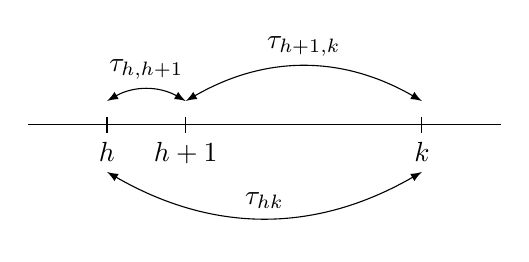
\begin{tikzpicture}
          % Line
          \draw[-] (-1,0) -- (5,0);
          % Integers
          \foreach \x/\label in {0/h, 1/h+1, 4/k} {
            \draw(\x,0.1) -- (\x,-0.1) node[below] {\(\label\)};
          }
          % Arcs above
          \draw[latex-latex, bend left=30] (0, 0.3) to node[midway, above] 
            {\(\tau_{h,h+1}\)} (1, 0.3);
          \draw[latex-latex, bend left=30] (1, 0.3) to node[midway, above]
            {\(\tau_{h+1,k}\)} (4, 0.3);
          % Arc below
          \draw[latex-latex, bend right=30] (0, -0.6) to node[midway, above]
            {\(\tau_{hk}\)} (4, -0.6);
        \end{tikzpicture}
    $$
    i.e.,
    $$
        \tau_{hk} = \tau_{h,h+1}\tau_{h+1,k}\tau_{h,h+1},
    $$
    and the conclusion follows by induction on $k-h$.
    \renewcommand{\qedsymbol}{\sc qed}
\end{proof}

Let $G=\gen{x_1,\dots,x_{n-1}\mid R}$, where $R$ stands for the relations listed above.

\paragraph{Claim 1:}$|G|\le n!$

By induction on $n$, the case $n=1$ is trivial. For $n>1$, let $G_{n-1}$ be like $G$ with $n-1$ replacing $n$. Similarly, let $R_{n-1}$ denote the relations for $n-1$. Hence,
$$
    G_{n-1}=\gen{x_1,\dots,x_{n-2}, R_{n-1}}
$$
By the inductive hypothesis we have $|G_{n-1}|\le (n-1)!$. Since $R_{n-1}\subseteq R$, we can use von Dyck's Theorem~\ref{von-dyck-thm} to conclude that there is an epimorphism $G\to G_{n-1}$. Hence, the claim will follow if we show that $|G:G_{n-1}|\le n$.

Since $\set{x_1,\dots,x_{n-1}}$ generates $G$, it is enough to verify that every $x_j$ permutes the $n$ right cosets
$$
    G_{n-1},\; G_{n-1}x_{n-1},\;\dots,\;G_{n-1}x_{n-1}\cdots x_1.
$$
For $1\le i\le n$ let $C_i$ denote the coset $G_{n-1}x_{n-1}\cdots x_i$. Note that $C_n=G_{n-1}$. There are five cases:
\begin{description}%[leftmargin=1.8cm,style=sameline]
    \item[$\underline{j<i-1}:$]
        \begin{align*}
            C_ix_j &= G_{n-1}x_{n-1}\cdots x_ix_j\\
                &= G_{n-1}x_jx_{n-1}\cdots x_i
                    &&;\ x_k\leftrightarrow x_j\\
                &= G_{n-1}x_{n-1}\cdots x_i
                    &&;\ x_j\in G_{n-1}\\
                &= C_i.
        \end{align*}
    \item[$\underline{j=i-1}:$] $C_ix_j=C_ix_{i-1}=C_{i-1}$.
    \item[$\underline{j=i}:$] Since $x_i^2=1$, $C_ix_j=C_ix_i=C_{i+1}$.
    \item[$\underline{j=i+1}:$]
        \begin{align*}
            C_ix_j &= C_ix_{i+1}\\
                &= C_{i+2}x_{i+1}x_ix_{i+1}\\
                &= C_{i+2}x_ix_{i+1}x_i
                    &&;\ (x_ix_{i+1})^3=1\\
                &= C_{i+2}x_{i+1}x_i
                    &&;\ i<(i+2)-1\\
                &= C_i.
        \end{align*}
    \item[$\underline{j>i+1}:$]
        \begin{align*}
            C_ix_j &= C_{j+1}x_jx_{j-1}x_{j-2}\cdots x_ix_j\\
                &= C_{j+1}x_jx_{j-1}x_jx_{j-2}\cdots x_i\\
                &= C_{j+1}x_{j-1}x_jx_{j-1}x_{j-2}\cdots x_i
                    &&;\ (x_{j-1}x_j)^3=1\\
                &= C_{j+1}x_jx_{j-1}x_{j-2}\cdots x_i
                    &&;\ j-1 < (j+1) -1\\
                &= C_i.
        \end{align*}
\end{description}

\paragraph{Claim 2:}$|G|\ge n!$

Let $\tau_{1,2},\dots,\tau_{n-1,n}$ be the $n-1$ adjacent permutations of $S_n$. Thus, the universal property of $G$ guaranties the existence of a commutative diagram
\begin{equation}\label{eq.G=S_n}
    \begin{tikzcd}
        {\set{x_1,\dots,x_{n-1}}}
                \arrow[d,"\tau"']
                \arrow[r,hook]
            &F
                \arrow[ld,"\tau^*"]
                \arrow[d,"\pi"]\\
        S_n
            &G
                \arrow[l,dashed,"\gamma"]
    \end{tikzcd}
\end{equation}
where $\tau(x_i)=\tau_{i,i+1}$. Given that, according to the lemma, $S=\gen{\im\tau}$, we deduce that $\tau^*$ is an epimorphism. Moreover, $\set{\tau_{12},\dots,\tau_{n-1,n}}$ satisfy the relations~$R$. Hence, by the von Dyck Theorem~\ref{von-dyck-thm}, the presentation $\pi$ induces an epimorphism $\gamma\colon G\to S_n$. In particular, $|G|\ge|S_n|=n!$.

\paragraph{Conclusion:} $\gamma:G\cong S_n$

This follows from the fact that $\im(\gamma)=S_n$, as shown by Claim~1 and Claim~2. Note also that, according to~$(\ref{eq.G=S_n})$, this isomorphism is the natural one that comes from the universal property of~$F$.

\end{proof}

\begin{xmpl}\label{example:group-of-order-21}
    Let $G$ be a nonabelian group or order $21$. Since $n_7(G)\mid3$ (Remark~\ref{p'-part}) and $n_7(G)\equiv 1\pmod 7$ (Corollary~\ref{p|n_p-1}), we deduce that there is only one subgroup $P$ of order $7$. Therefore $P\normal G$. If $Q\in\Syl_3(G)$, then $G=PQ$. Since $G$ is not abelian and both $P$ and $Q$ are cyclic, $n_3(G)>1$, otherwise $Q$ would be normal and consequently $P\leftrightarrow Q$. Since $n_3(G)\mid 7$, we deduce that $n_3(G)=7$.

    Given that $\Aut(\Z_7)$ is cyclic of order $7-1$, it contains $2$ elements of order~$3$, namely $\eta_2\colon x\mapsto 2x$ and $\eta_4\colon x\mapsto4x$, with $\eta_4=\eta_2^{-1}$. Therefore, there are two nontrivial morphisms from $\Z_3$ to $\Aut(\Z_7)$, one is $\phi_1\colon1\mapsto\eta_2$ and the other $\phi_2\colon 1\mapsto\eta_2^{-1}$.

    Consider the inversion $\tau\colon\Z_3\to\Z_3$ defined by $\tau(x)=-x$. Then $\phi_1\tau=\phi_2$ because
    $$
        \phi_1\tau(1)=\phi_1(-1)=\phi_1(1)^{-1}=\eta_2^{-1}(1)=\phi_2(1).
    $$
    Now define
    \begin{align*}
        \Phi\colon\Z_7\rtimes_{\phi_1}\Z_3&\to\Z_3\rtimes_{\phi_2}\Z_3\\
            (a,b)&\mapsto(a,\tau(b)).
    \end{align*}
    We have,
    \begin{align*}
        \Phi((a_1,b_1)\cdot_{\phi_1}(a_2,b_2))
            &= \Phi(a_1\phi_1(b_1)(a_2),b_1b_2)\\
            &= (a_1\phi_1(b_1)(a_2),\tau(b_1b_2))\\
            &= (a_1\phi_2(\tau(b_1))(a_2),\tau(b_1)\tau(b_2))
                &&;\ \tau^2=\id\\
            &= (a_1,\tau(b_1))\cdot_{\phi_2}(a_2,\tau(b_2))\\
            &= \Phi(a_1,b_1)\cdot_{\phi_2}\Phi(a_2,b_2),
    \end{align*}
    i.e., $\Phi$ is a morphism. Hence, an isomorphism. In conclusion, there is only one nonabelian group or order $21$, up to isomorphism [cf.~Lemma~\ref{semidirect-product-uniqueness}].

    Let now $B$ the group defined with generators and relations
    $$
        B = \gen{\sigma,\tau\mid \sigma^7=\tau^3=1,\,\sigma^2\tau=\tau\sigma}.
    $$
    Note that $\Z_7\rtimes\Z_3$ satisfies the same relations, for $\sigma=(1,0)$ and $\tau=(0,1)$. We can verify this using $\phi_1$ defined above,
    \begin{align*}
        \sigma^2\tau &= (1,0)(1,0)(0,1)\\
            &= (2,0)(0,1)\\
            &= (2,1)\\
        \tau\sigma &= (0,1)(1,0)\\
            &= (0+\eta_2(1),1)\\
            &= (2,1).
    \end{align*}
    By the von Dyck Theorem~\ref{von-dyck-thm}, there is an epimorphism $\pi\colon B\to\Z_7\times\Z_2$ that extends the map $\sigma\mapsto(1,0)$, $\tau\mapsto(0,1)$. Given that the products $\sigma^i\tau^j$ generate a subgroup that is normal in the free group, these products generate $B$. This implies that $\pi$ is a monomorphism because the exponents $i$ and $j$ are univocally determined in $\Z_7\rtimes\Z_3$.
\end{xmpl}


\chapter{Subnormality}
\section{Minimal Normal Subgroups}

\begin{defn}\label{socle-defn}
    The \textsl{socle} of a finite group\/ $G$ is the subgroup $\Soc(G)$ generated by all minimal normal subgroups of\/ $G$, i.e.,
    $$
        \Soc(G) = \prod\Nm(G),
    $$
    where\/ $\Nm(G)$ denotes the family of all minimal normal subgroups. Here, of course, \textsl{minimal} implies nontrivial. In particular, $\Soc\gen1=\prod\emptyset=\gen1$.
\end{defn}

\begin{rems}\label{soc-intersection}${}$
    \begin{enumerate}[\rm i)]
        \item If $N$ is normal and nontrivial, then $N$ includes some minimal normal group and therefore $N\cap\Soc(G)\ne\gen1$.
        \item $\Soc(G)$ is characteristic\/\textrm{\rm: automorphisms preserve inclusions and normality.}
        \item $G$ simple $\implies\Soc(G) = G$.
        \item $\Soc(G)$ can be expressed as the direct product of a subfamily of\/ $\Nm(G)$\textrm{\rm: a running direct product of minimal normal subgroups only increases with the next minimal normal subgroup when such a subgroup has trivial intersection with said product [cf.~Theorem~\ref{product-of-minimal-normal}].}
    \end{enumerate}
\end{rems}

\begin{ntn}
    We will write $M\normal_m G$ to indicate that $M$ is minimal normal in~$G$.
\end{ntn}


\begin{prop}
    Let\/ $M$ be a minimal normal subgroup of\/ $G$.
    \begin{enumerate}[\rm a)]
        \item If\/ $N\normal G$ then\/ $M \subseteq N$ or\/ $M \cap N = \gen1$. In the latter case, $[M, N] = \gen1$.
        \item If\/ $M$ is abelian then\/ $M \subseteq H$ or\/ $M \cap H = \gen1$ for any subgroup\/ $H$ of\/ $G$ with\/ $G = MH$.
        \item If\/ $\phi\colon G\to H$ is an epimorphism then\/ $\phi(M) = \gen1$ or\/ $\phi(M)\normal_mH$.
    \end{enumerate}
\end{prop}

\begin{proof}${}$
\begin{enumerate}[\rm a)]
    \item Since $M\cap N\normal_mG$, the first conclusion is a direct consequence of the definition. The second simply says that $M\leftrightarrow N$ when $M\cap N=\gen1$.

    \item By Remark~\ref{abelian-normal}, $M\cap H\normal MH=G$. The conclusion follows because $M\cap H\subseteq M$.

    \item By Proposition~\ref{image-of-normalizer} we get $\phi(M)\normal H$. Suppose that $\phi(M)\ne\gen1$. Take $L\normal H$ satisfying $L\subseteq\phi(M)$. Then $\phi^{-1}(L)\normal G$ by Remark~\ref{biunivocal-normal-quotient}. Since $\phi^{-1}(L)\cap M\normal G$ is a subgroup of $M$, $\phi^{-1}(L)=\gen1$ or $M\subseteq\phi^{-1}(L)$. In the first case, $L=\phi(\phi^{-1}(L))=\gen1$. In the second, $\phi(M)\subseteq\phi(\phi^{-1}(L))=L$.
\end{enumerate}
\end{proof}

\begin{thm}\label{product-of-minimal-normal}
    Let\/ $\mathcal N\subseteq\Nm(G)$ be a finite set of minimal normal subgroups of\/ $G$ and let
    $$
        X = \prod\mathcal N.
    $$
    \begin{enumerate}[\rm a)]
    \item If\/ $N$ is a normal subgroup of\/ $G$, then there exist\/ $M_1, \dots, M_n \in\mathcal N$ such that
    $$
        NX = N \times M_1 \times \cdots \times M_n.
    $$
    \item There exist\/ $M_1, \ldots, M_r \in\mathcal N$ such that
    $$
        X = M_1 \times \cdots \times M_r.
    $$
    \end{enumerate}
\end{thm}

\needspace{2\baselineskip}
\begin{proof}${}$
\begin{enumerate}[\rm a)]
    \item Take a maximal subset $\cal L$ of $\mathcal N$ such that $Q=N\prod\cal L$ is a direct product. If $Q\ne NX$ there must exist $M\in\mathcal N$ such that $M\not\subseteq Q$. Since $M\normal_mG$ and $Q\normal G$ it follows that $Q\cap M=\gen1$. According to Theorem~\ref{direct-product} this implies that $QM$ is a direct product, contradicting the maximality of~$\cal L$.

    \item This is nothing but a) applied to $N=\gen1$.
\end{enumerate}
\end{proof}


\begin{cor}\label{minimal-normal-of-minimal-normal}
    Let\/ $N$ be minimal normal in\/ $G$ and\/ $M$ minimal normal in\/~$N$. Assume that the set\/ $\set{M^x \mid x \in G}$ is finite. Then\/ $M$ is simple and there exist\/ $x_1, \dots, x_n$ in\/ $G$ such that
    \begin{equation}\label{eq1.7}
        N = M^{x_1} \times \cdots \times M^{x_n}.
    \end{equation}
\end{cor}

\begin{proof} The product $\prod_{x\in G}M^x$ is a subgroup of $N$ because $M^x\normal N^x=N$ for $x\in G$. And given that it is normal in $G$, it must equal $N$. By the theorem, equation $(\ref{eq1.7})$ is attained for some $x_1,\dots,x_n\in G$. In particular, $M^{x_i}\leftrightarrow M^{x_j}$ for $i\ne j$. Therefore, given $L\normal M$, we get $L^{x_1}\normal M^{x_1}$ with $L^{x_1}\leftrightarrow M^{x_i}$ for $i\ne 1$. Thus, $L^{x_1}\normal N$. It follows that $L\normal N$, which implies that $L$ is trivial or $M$ because $L\subseteq M$ and $M\normal_mN$.  \end{proof}

\begin{cor}\label{abelian-minimal-normal-is-elementary}
    Let\/ $A$ be an abelian minimal normal subgroup of the finite group\/ $G$. Then there exists a prime\/ $p$ such that\/ $A$ is a direct product of subgroups that are isomorphic to\/ $\Z_p$.
\end{cor}

\begin{proof} In the case where $A$ is abelian, $M\normal_mA\iff M\cong\Z_p$ for some prime $p\mid|A|$. Thus, the previous corollary implies that $A$ is a direct product of copies of~$\Z_p$.  \end{proof}

\begin{defn}
    Let\/ $G$ be a group. A subgroup\/ $H$ is said to be \textsl{subnormal} in\/ $G$ when there exists a finite sequence
    $$
        H = H_0 \normal H_1 \normal \cdots \normal H_r = G.
    $$
    In such a case we write $H\snormal G$.
\end{defn}

\begin{thm}\label{semisimple-normal}
    Let\/ $G = G_1 \times \cdots \times G_n$ and\/ $N$ a normal subgroup of\/ $G$.
    \begin{enumerate}[\rm a)]
    \item If\/ $N$ is perfect, then\/ $N = (N \cap G_1) \times \cdots \times (N \cap G_n)$.
    \item If\/ $G_1, \dots, G_n$ are nonabelian simple groups, then\/ $N$ is perfect and there exists a subset\/ $J \subseteq \nset n$ such that
    $$
        N = \prod_{j \in J} G_j\quad\text{\rm and}\quad G_k \cap N = 1\text{\rm\ for }k \notin J.
    $$
    \item If\/ $G_1, \dots, G_n$ are nonabelian simple groups and\/ $H\snormal G$, then\/ $H\normal G$, and part\/~{\rm b)} applies on\/ $H$ as well.
    \end{enumerate}
\end{thm}

\needspace{2\baselineskip}
\begin{proof}${}$
\begin{enumerate}[\rm a)]
    \item By Proposition~\ref{commutator-props} we have
    $$
        N=N'=[N,N]\subseteq[N,G] = \prod_{i=1}^n[N,G_i]\subgroup\prod_{i=1}^nN\cap G_i
            \subseteq N.
    $$
    \item By part a) it suffices to show that $N$ is perfect. We will prove this by induction on $n$.

    The case $n=1$ is trivial because $N=G_1$ is perfect. Let's assume that $n>1$.
    
    If $N=G$ there is nothing to prove. Assume $N\ne G$. Then there exists $k$ such that $G_k\not\subseteq N$. Since $N\cap G_k\normal G_k$, by simplicity $N\cap G_k=\gen1$. Put $\bar N=NG_k/G_k$, $\bar G_i=G_iG_k/G_k$ and $\bar G=G/G_k$.

    Note that $\bar G_i\cong G_i$ for $i\ne k$, and therefore $\bar G_i$ is simple and nonabelian. Moreover,
    $$
        \bar G = \prod_{i\ne k}\bar G_i
    $$
    because, for $i\ne j$ both different from $k$, we have
    \begin{align*}
        \bar x\in \bar G_i\cap \bar G_j &\iff x\in G_iG_k\cap G_jG_k\\
            &\iff x\in G_k   &&\text{; Thm.~\ref{direct-product}}\\
            &\iff \bar x= 1.
    \end{align*}
    Since $\bar N\normal\bar G$, the inductive hypothesis implies that $\bar N$ is perfect. Therefore,
    $$
        N\cong NG_k/G_k = (NG_k/G_k)' = N'G_k/G_k \cong N',
    $$
    where both isomorphisms hold because $N'\cap G_k\subseteq N\cap G_k=\gen1$. Then $|N|=|N'|$, and the inclusion $N'\subseteq N$ implies $N=N'$.

    \item It is enough to show that $H$ is decomposable as a direct product of a subfamily of the $G_i$. Take a sequence
    $$
        H=H_0\normal H_1\normal\cdots\normal H_r=G.
    $$
    If $r\le 1$ then $H\normal G$ and we are done. If $r>1$ then $H_{r-1}\normal G$. Therefore, according to part~b), $H_{r-1}$ is decomposable as the direct product of a subfamily of the $G_i$. By induction on $r$, we deduce that $H$ is the direct product of a subsubfamily of the $G_i$.
\end{enumerate}
\end{proof}

\begin{cor}
    Let\/ $N$ be a nonabelian minimal normal subgroup of the finite group\/ $G$.  Then
    \begin{enumerate}[\rm a)]
        \item The elements of\/ $\Nm(N)$ are nonabelian simple groups, which are conjugate in\/ $G$.
        \item $N = \bigtimes\Nm(N)$.
        \item For every\/ $M\normal N$ the collection
        $$
            \Nm(N;M)=\set{L\in\Nm(N)\mid L\subseteq M}
        $$
        satisfies
        $$
            \Nm(N;M) = \Nm(M).
        $$
        In particular,
        $$
            M = \bigtimes\Nm(N;M)
        $$
    \end{enumerate}
\end{cor}

\needspace{2\baselineskip}
\begin{proof}${}$
\begin{enumerate}[\rm a)]
    \item Take $M\in\Nm(N)$. Corollary~\ref{minimal-normal-of-minimal-normal} implies that $M$ is simple and that equation~$(\ref{eq1.7})$ holds. In particular $M$ is nonabelian. If $L$ is another element in $\Nm(N)$, from part~b) of Theorem~\ref{semisimple-normal} (applied to $G=N$ and $N=L$) we deduce that $L$ is a direct product of some of the factors $M^{x_i}$ occurring in~$(\ref{eq1.7})$. But given that $L\normal_mN$, such product can only have one factor, i.e., $L$ and $M$ are conjugate in $G$.

    \item Firstly note that the product $\prod\Nm(N)$ is direct. In addition, according to Corollary~\ref{minimal-normal-of-minimal-normal}, it equals $N$.

    \item By definition $\Nm(N;M)\subseteq\Nm(M)$. To verify the other inclusion take $L\in\Nm(M)$. Then $L\normal_m M\normal N$. It follows that $L\snormal N$. Thus, according to part~c) of Theorem~\ref{semisimple-normal}, $L\normal N$ and so $L\in\Nm(N;M)$. The last equality now follows from part~b) of the same theorem for $G=N$ and $N=M$.
\end{enumerate}
\end{proof}

\subsection{Exercises - Kurzweil \& Stellmacher - \S 1.7}

\begin{exr}
     Let\/ $G$ be a finite group and\/ $M$ a maximal subgroup of\/ $G$. All minimal normal subgroups\/ $N$ of\/ $G$ that satisfy\/ $N\cap M=\gen1$ are isomorphic.
\end{exr}

\begin{solution} {[See also \href{https://math.stackexchange.com/a/2694761/269050}{this MSE answer}]} Let's say that a subgroup $X$ of $G$ is \textsl{good\/} if $X\normal_mG$ and $X\cap M=\gen1$. If $X$ is good then $G=XM$ and $M\cong G/X$. Let $N$ and $L$ be two good subgroups of $G$. To show that $N\cong L$ we may assume that $N\ne L$. It follows that $N\cap L=\gen1$ and, consequently, $N\leftrightarrow L$. Let `$\sim$' be the relation on $N\times L$ defined as
\begin{equation}\label{eq1.7.1}
    a \sim b\iff ab\in M.
\end{equation}
Given $a\in N$ we can write $a=zb$ with $b\in L$ and $z\in M$. Thus, $ab^{-1}=z\in M$, i.e., $a\sim b^{-1}$. In particular, $\dom(\sim)=N$.

If $a\sim b_1$ and $a\sim b_2$, by definition, both $ab_1$ and $ab_2$ belong to $M$, which implies
$$
    b_1^{-1}b_2 = b_1^{-1}a^{-1}ab_2 = (ab_1)^{-1}(ab_2)\in M.
$$
Since $b_1b_2^{-1}$ is clearly in $L$, we get $b_1^{-1}b_2\in M\cap L=\gen1$, i.e., $b_1=b_2$. Thus, the relation is actually a function from $N$ to $L$.

To verify that $\sim$ is a morphism of groups take $a_1\sim b_1$ and $a_2\sim b_2$. Then
$$
    (a_1a_2)(b_1b_2) = (a_1b_1)(a_2b_2)\in M,
$$
i.e., $a_1a_2\sim b_1b_2$.

The morphism is mono because $a\sim 1$ means $a\in M$, which implies $a=1$. It is epi because given $b\in L$ we can write $b^{-1}=za$ for appropriate $z\in M$ and $a\in N$ which implies $ab=z^{-1}\in M$, i.e., $a\sim b$.

In sum, $(\ref{eq1.7.1})$ defines an isomorphism from $N$ onto $L$.  \end{solution}

\begin{exr}
    Let\/ $G$ be a finite group and\/ $M$ a maximal subgroup of\/ $G$. If\/ $M$ is nonabelian and simple, then there exist at most two minimal normal subgroups in\/~$G$.
\end{exr}

\begin{solution} Let $N\normal_mG$, $N\ne M$. Since $N\cap M\normal M$, we get $N\cap M=\gen1$. If $L\normal_mG$, $L\ne N$, then $NL/N\normal G/N$. But $G/N\cong M$ is simple and so $G=NL$, where the product is direct because $N\cap L=\gen1$. In addition, $N\cong NL/L\cong M$ is simple and the same goes for $L$. Should $H$ be minimal normal, Theorem~\ref{semisimple-normal} would imply $H=N$ or $H=L$. 

{\small \textbf{Another approach:} [\href{https://math.stackexchange.com/a/1188536/269050}{From a comment by Derek Holt}] Since $N\cap L=\gen1$, $N\leftrightarrow L$ and so $L\subseteq C_G(N)$. But equality is attained because $C_G(N)\cap N\normal N$ and $N\cong M$ is simple and nonabelian, which implies that $C_G(N)\cap N=\gen1$. Therefore, $L=C_G(N)$ is determined by~$N$.}

 \end{solution}

\begin{exr}
    In the conditions of the preceding exercise, give an example where\/ $G$ possesses two minimal normal subgroups.
\end{exr}


\begin{exr}
    Let\/ $G$ be a finite group and\/ $M$ a maximal subgroup of\/ $G$. Suppose that\/ $G$ contains two minimal normal subgroups, neither of which is contained in\/ $M$. Then every minimal normal subgroup of\/ $M$ is contained in\/ $\Soc(G)$, the product of all minimal normal subgroups of\/ $G$.

    \textrm{\rm Hint [l.c.]: Let $X\not\subseteq M$, $X\normal_m G$. Then $H\normal_m M\implies HX/X\normal_mG/X$. Also show that $[H,X]\normal G$.}
\end{exr}

\begin{solution} {[Brought from \href{https://math.stackexchange.com/a/1220274/269050}{MSE}]} Take $H\normal_mM$ and suppose that $H\not\subseteq\Soc(G)$. One first conclusion we can draw is that $H\cap\Soc(G)=\gen1$. In particular, 
\begin{equation}\label{eq1.7.4}
    H\nnormal G,
\end{equation}
otherwise, $H$ would contain a minimal normal subgroup of $G$.

Let's say that a subgroup $X$ of $G$ is \textsl{good} if $X\normal_mG$ and $X\not\subseteq M$. The hint's proof is divided into three claims. Bellow we will refer to two different good subgroups~$X$ and~$Y$, whose existence is a hypothesis.

\needspace{2\baselineskip}
\textbf{Claim 1:} $HX\normal G$

{\small Since $G=XM$, to prove the claim it is enough to verify that both $X$ and $M$ normalize $HX$. But this is clear because, for every $x\in X$, $(HX)^x\subseteq HX$ and, on the other hand, $M$ normalizes both $H$ and $X$.}

\medskip

\needspace{2\baselineskip}
\textbf{Claim 2:} $HX/X\normal_mG/X$

{\small Take $K\normal G$ be such that $X\subseteq K\subseteq HX$. To prove the claim we have to show that $K=X$ or $HX$. There are two possibilities $K\cap H=H$ or $\gen1$. The first means that $H\subseteq K$ and we are done. Thus, we may assume that $K\cap H=\gen1$. Given $b\in K$, write $b=ax$ for some $a\in H$ and $x\in X\subseteq K$. Then $a=bx^{-1}\in H\cap K=\gen1$, which implies that $b=x\in X$. Since $b$ was arbitrarily chosen and $X\subseteq K$, we deduce that $K=X$.}

\medskip

\textbf{Claim 3:} $[H,Y]\normal G$

{\small Since $Y\leftrightarrow X$ and $[H,Y]\subseteq Y$, we obtain $[H,Y]\leftrightarrow X$. In particular, $X$ normalizes $[H,Y]$. And since $M$ also normalizes $[H,Y]$, from the equation $G=XM$ we conclude that $[H,Y] \normal G$.
}

\medskip

\textbf{Claim 4:} $[H,Y]=Y$ and $[H,Y]X/X= HX/X$.

{\small Take $a\in H$, $y\in Y$. Write $y=xz$ with $z\in M$. We have
$$
    [a,y]=aya^{-1}y^{-1}=axza^{-1}z^{-1}x^{-1}
        = ax(a^{-1})^zx^{-1}\in HX.
$$
Therefore $[H,Y]X\subseteq HX$, which implies $[H,Y]X/X\subseteq HX/X$. 

Should $H\leftrightarrow Y$, both $Y$ and $M$ would normalize $H$ and so $H\normal G$, in contradiction with~($\ref{eq1.7.4}$). It follows that $[H,Y]$ is a nontrivial subgroup of $Y$.

Now observe that $[H,Y]\subseteq Y$. Since $\gen1\ne[H,Y]\normal G$ we get $[H,Y]=Y$ and $[H,Y]X/X=HX/X$ (by Claim~2).}

\medskip

\textbf{Conclusion.} From Claim 4 we deduce
$$
    HX/X=[H,Y]X/X = YX/X,
$$
i.e., $HX=YX$. It consequence,
$$
    H \subseteq HX = YX\in\Soc(G),
$$
which contradicts our initial assumption.  \end{solution}

\begin{exr}
    Let's say that a group is \textsl{good} whenever every minimal normal subgroup is contained in the center. Let\/ $G$ be good.
    \begin{enumerate}[\rm a)]
    \item If\/ $N$ and\/ $M$ are good normal subgroups of\/ $G$, then\/ $NM$ is good.
    \item Every normal subgroup of\/ $G$ is good.
    \end{enumerate}
\end{exr}

\begin{solution}
\begin{enumerate}[\rm a)]
    \item Fix any $H\normal_mNM$.
    
    \textbf{Claim 1: } $H\subseteq N\implies H\subseteq Z(N)$.
    
    {\small Assume that $H\subseteq N$ and pick $A\normal_mN$, $A\subseteq H$. By hypothesis $A\subseteq Z(N)$. Moreover, given $y\in M$, we have $A^y\normal N^y=N$. It follows that $A^M\normal N$. But $M$ normalizes $A^M$ and so $A^M\normal NM$. Since $A^M\subseteq H^M=H\normal_m NM$, we get $A^M=H$. Hence, to show that $H\subseteq Z(N)$ it is enough to verify that $A^y\subseteq Z(N)$. But this is clear because $Z(N)\ch N\normal G$ implies that $A^y\subseteq Z(N)^y=Z(N)$.}

    \medskip

    \textbf{Claim 2:} $H\subseteq N\implies H\subseteq Z(NM)$

    {\small Assume that $H\subseteq N$. If ---in addition--- $H\subseteq M$, Claim~1 applied to $M$ implies that $H\subseteq Z(M)$. It follows that $H\subseteq Z(NM)$. Otherwise, if $H\not\subseteq M$, given that both $H$ and $M$ are normal in $NM$, we deduce that $H\cap M=\gen1$ and so $H\leftrightarrow M$. Therefore, in this case we also have $H\subseteq Z(NM)$.}

    \medskip

    \textbf{Conclusion:} Claims 1 and 2 reduce the question to the case $H\cap N=\gen1$. By the symmetry between $N$ and $M$ we may also assume that $H\cap M=\gen1$. But then $H\leftrightarrow N$ and $H\leftrightarrow M$, which implies $H\subseteq Z(NM)$.

    \item {[Brought from \href{https://math.stackexchange.com/a/2703032/269050}{MSE}]} Let $N$ be a normal subgroup of $G$. Take $H\normal_mN$. Since $H^x\normal_mN^x=N$ for $x\in G$, we get $H^G\subgroup N$ with $H^G\normal G$. Take $A\normal_mG$, $A\subseteq H^G$. By hypothesis, $A\subseteq Z(G)$. By Theorem~\ref{product-of-minimal-normal}, we can write $H^G$ as a direct product
    $$
        H^G = H^{x_1}\cdots H^{x_n}.
    $$
    Pick $a\in A\setminus\set1$ and write it as
    $$
        a=c_1^{x_1}\cdots c_{n}^{x_n}
            \in H^{x_1}\times\cdots\times H^{x_n}.
    $$
    Since $a\ne1$, we may assume that $c_1^{x_1}\ne1$. Take $y\in N$, we have
    $$
        a = a^y = (c_1^{x_1})^y\cdots (c_n^{x_n})^y
    $$
    and so $(c_i^{x_i})^y=c_i$, i.e., $c_i^{x_i}\leftrightarrow y$ for all $i$. In particular, $c_1^{x_1}\leftrightarrow y$. Since $y$ was arbitrarily chosen, $1\ne c_1^{x_1}\in H^{x_1}\cap Z(N)$. Recalling that $H^{x_1}\normal_mN$, we get $H^{x_1}\subseteq Z(N)$ and therefore $H\subseteq Z(N)$ because $Z(N)\ch N\normal G$.
\end{enumerate}
\end{solution}


\section{Subnormal Subgroups}
\begin{defn}
    Let's recall that a subgroup\/ $H$ of a group\/ $G$ is subnormal when there exists a finite sequence
    $$
        H = H_0 \normal H_1 \normal \cdots \normal H_r = G.
    $$
    In such a case the smallest value of\/ $r$ for which such a sequence exists is the \textsl{subnormality depth} of\/ $H$, denoted by $\sd_G(H)$.
\end{defn}

\begin{rem}
    Note that when $H\snormal G$ the sequence can be chosen to be strictly increasing. Unlike normality, subnormality is a transitive relation.
\end{rem}

\begin{rem}
    Let\/ $N\subseteq H$ be subgroups of the group\/ $G$. If $N\normal G$ and the quotient $H/N$ is subnormal in $G/N$, then $H\snormal G$.
\end{rem}

\begin{lem}\label{nilpotent-lemma}
    Let\/ $G$ be finite. Then\/ $G$ is nilpotent if, and only if, every subgroup of\/ $G$ is subnormal.
\end{lem}

\begin{proof}${}$

\begin{description}
    \item[\rm\textit{if\/} part)] Let $H$ be a subgroup. Since $H\snormal G$, there is a strictly increasing sequence from $H$ to $G$, say $H\normal H_1\normal\cdots\normal H_r=G$. In particular, $H\varsubsetneq H_1\subseteq N_G(H)$. The conclusion now follows from Theorem~\ref{nilpotent-equivalences}.

    \item[\rm\textit{only if\/})] The same theorem implies that $H\varsubsetneq N_G(H)$. Put $H_1=N_G(H)$. If we repeat the same construction defining $H_{i+1}=N_G(H_i)$, we will eventually reach $G$.
\end{description}
\end{proof}

\begin{xmpl}
    The \textsl{Klein subgroup} of\/ $S_4$ can be represented by the three $2$-cycles, plus the identity 
    $$
        K = \set{(),(1 2)(3 4), (1 3)(2 4), (1 4)(2 3)}.
    $$
    \begin{enumerate}[\rm i)]
        \item The group is abelian{\rm: $K$ is the identity plus all elements in $S_4$ with order $2$ and sign $1$. Therefore, for $a$, $b$ and $c$ in $K$, $ab=c\ne()\implies ba=c$.}
        
        \item $K$ is normal{\rm: Indeed, conjugation preserves order and sign.}
        
        \item If\/ $H\subseteq K$, $|H|=2$, then $|N_{S_4}(H)|=8${\rm: $H\varsubsetneq N_{S_4}(H)$ because\/ $(ab)\in H$ implies $(cd)(ab)(cd)=(ab)$, which shows the existence of\/ $1$ additional element in\/ $N_{S_4}(H)$. Thus, $|N_{S_4}(H)|\ge3$, and so\/ $N_{S_4}(H)\ge4$. Since $(acd)(ab)(dca)=(bd)$, there is at least $1$ element of order $3$ that doesn't belong to $N_{S_4}(H)$. Given that $H\normal K$ because $K$ is abelian, we have $K\subseteq N_{S_4}(H)$. Moreover, the inclusion is strict because $(cd)$ is not in $K$. It follows that $|N_{S_4}(H)|=8$.}
    
        \item $H\snormal S_4${\rm: Since\/ $K$ is abelian, $H\normal K$ and by ii) $K\normal S_4$.}
    
        \item $N_{S_4}(H)\nnormal S_4${\rm: $N_{S_4}(H)\in\Syl_2(S_4)$ and $n_2(S_4)=|S_4:N_{S_4}(H)|=3$.}
    \end{enumerate}
    As a result, $H\snormal S_4$ but we cannot reach $S_4$ from $H$ taking stabilizers.
\end{xmpl}

\begin{thm}\label{nilpotent-and-subnormal}
    Let\/ $G$ be a finite group and\/ $H$ a subgroup. Then $H\subseteq F(G)$ if, and only if, $H$ is nilpotent and subnormal in\/ $G$.
\end{thm}

\needspace{1\baselineskip}
\begin{proof}${}$

\begin{description}
    \item[\rm{\it if\/} part)] By induction on $|G:H|$, the case $|G:H|=1$ is trivial because it happens when $H=G$, i.e., when $G$ is nilpotent, i.e., when $G=F(G)$ [cf.~Corollary~\ref{normal-nilpotent-fitting}]. Let $H_{r-1}$ be the next-to-last group in a strictly growing normal chain from $H$ to $G$. Since $|H_{r-1}:H|< |G:H|$, we can apply the inductive hypothesis and conclude that $H\subseteq F(H_{r-1})$. But $F(H_{r-1})\ch H_{r-1}\normal G$. Therefore, we can invoke Lemma~\ref{normal-transitivity} to get $F(H_{r-1})\normal G$. Then, $F(H_{r-1})\subseteq F(G)$ by the same corollary. Ergo, $H\subseteq F(G)$.

    \item[\rm{\it only if\/})] First observe that $H$ is nilpotent because $H\subseteq F(G)$ and any subgroup of a nilpotent group is nilpotent by Corollary~\ref{nilpotent-subgroups-and-quotients}. By Lemma~\ref{nilpotent-lemma}, $H$ is subnormal in $F(G)$. Since $F(G)\normal G$, the conclusion follows by subnormal transitivity.
\end{description}
\end{proof}

\begin{lem}\label{subnormal-restriction}
     If\/ $H \snormal G$ and $K \subgroup G$, then $H\cap K \snormal K$.
\end{lem}

\begin{proof} Take a normal sequence $H=H_0\normal H_1\normal\cdots\normal H_r=G$. By Proposition~\ref{prod-quotient}, $H_{i-1}\cap K\normal H_i\cap K$ for $i=1\dots r$. Therefore, the intersected chain is a normal chain from $H\cap K$ to $K$.  \end{proof}

\begin{prop}
    Let\/ $G$ be a group, and\/ $H$ and\/ $K$ subnormal in\/ $G$. Then $H\cap K$ is subnormal in\/~$G$.
\end{prop}

\begin{proof} This is a direct consequence of the lemma and the transitivity of subnormality because $H\cap K\snormal K\snormal G$.  \end{proof}


\begin{thm}\label{minimal-normal-normalizes-subnormal}
    Let\/ $H\snormal G$, where\/ $G$ is a finite group, and let $M\normal_mG$. Then $M \subseteq N_G(H)$. In other words, $\Soc(G)\subseteq N_G(H)$.
\end{thm}

\begin{proof} It proceeds by induction on $|G:H|$. If $|G:H|=1$, then $H=G$ is normal and there is nothing to prove. Take a strictly growing normal chain from $H$ to $G$ and let $H_{r-1}$ be its next-to-last subgroup. Let's analyze two cases:
\begin{description}
    \item[\small${[}M\cap H_{r-1}=\gen1{]}$] Since both $M$ and $H_{r-1}$ are normal, $MH_{r-1}=M\times H_{r-1}$. In particular [cf.~Theorem~\ref{direct-product}] $M\leftrightarrow H_{r-1}$ and so
    $$
        M \subseteq C_G(H_{r-1})\subseteq C_G(H) \subseteq N_G(H).
    $$
    
    \item[\small${[}M\cap H_{r-1}\ne\gen1{]}$] Firstly, $M\cap H_{r-1}$, being normal, must equal $M$ because $M$ is minimal with that property. Thus, $M\subseteq H_{r-1}$ and so $M\normal H_{r-1}$. 
    
    Secondly, the inductive hypothesis implies that $\Soc(H_{r-1})\subseteq N_{H_{r-1}}(H)$. Since $N_{H_{r-1}}(H)\subseteq N_G(H)$, it follows that $\Soc(H_{r-1})\subseteq N_G(H)$.
    
    Finally, $\gen1\ne M\normal H_{r-1}$. Hence, $M\cap\Soc(H_{r-1})\ne\gen1$ by Remark~\ref{soc-intersection}. Since $\Soc(H_{r-1})\ch H_{r-1}\normal G$, by Lemma~\ref{normal-transitivity}, we obtain $\Soc(H_{r-1})\normal G$. Then $M\cap\Soc(H_{r-1})\normal G$. But $M\cap\Soc(H_{r-1})\subseteq M$ and therefore, $M\cap\Soc(H_{r-1})=M$. Therefore, $M \subseteq \Soc(H_{r-1})\subseteq N_G(H)$.
\end{description}
\end{proof}

\begin{thm}\label{subnormal-lattice}
    If\/ $G$ is a finite group, the collection of its subnormal subgroups is a lattice.
\end{thm}

\begin{proof} It suffices to show that if $H,\,K \snormal G$ then\/ $\gen{H,K} \snormal G$. The proof works by induction on $|G|$. The case $|G|=1$ is trivial, so we proceed with the case $|G|>1$. Let $M$ be a minimal normal subgroup of $G$. Consider the quotient $\bar G=G/M$ and the images $\bar H$ and $\bar K$ on it. The inductive hypothesis implies that $\gen{\bar H,\bar K}\snormal\bar G$. It follows that $\gen{H,K}M\snormal G$. By Theorem~\ref{minimal-normal-normalizes-subnormal}, we have $M\subseteq N_G\gen{H,K}$. Then $\gen{H,K}\normal \gen{H,K}M\snormal G$.  \end{proof}

\begin{thm}\label{zipper-lemma} {\rm[Zipper Lemma]}
    Suppose that\/ $H$ is a subgroup of a finite group\/ $G$ and assume that\/ $H\snormal K$ for every proper subgroup\/ $K$ of\/ $G$ that contains\/ $H$. If\/ $H$ is not subnormal in\/ $G$, then there is a unique maximal subgroup of\/ $G$ that contains\/ $H$.
\end{thm}

\begin{proof} Let's work by induction on $|G:H|$. If $|G:H|=1$, then $H=G$ and there is nothing to prove. Consider the case $|G:H|>1$. We may suppose that $H$ is not subnormal in $G$. In particular $N_G(H)\varsubsetneq G$ and there exists $M$ maximal such that $N_G(H)\subseteq M$. Thus, to complete the proof, it is enough to show that no other maximal includes $H$. Suppose otherwise and let $L$ be such other maximal. By hypothesis $H\snormal L$.

If $H\normal L$, then $L\subseteq N_G(H)\subseteq M$, i.e., $L=M$ and we are done.

We are left with the case $H\not\normal L$. It follows that any normal chain from $H$ to $L$ with the shortest length, say
$$
    H = H_0\normal H_1\normal\cdots\normal H_{r-1}\normal H_r = L,
$$
has $r\ge 2$. Note also that $H\not\normal H_2$, otherwise we could remove $H_1$ and get a shorter chain. Pick $x\in H_2$ so that $H^x\ne H$ and put $J=\gen{H,H^x}$. Since $H^x\subseteq H_1^x = H_1$, we have
$$
    J\subseteq H_1\subseteq N_G(H) \subseteq M.
$$
Let's say (within the scope of this proof) that a subgroup of $G$ is \textsl{good} when it satisfies the hypothesis of the theorem. Of course, $H$ is good. And given that every conjugation is an automorphism, $H^x$ is good too. We claim that $J$ is also good.

To verify the claim, let $K$ be a proper subgroup containing $J$. Then $H,\,H^x\subseteq K$ and therefore, $H\snormal K$ and $H^x\snormal K$ (both subgroups are good). By Theorem~\ref{subnormal-lattice}, $J\snormal K$ as needed.

Note also that $J$ is not subnormal in $G$, otherwise $H\normal J\snormal G$ and $H$ would be subnormal in $G$, which isn't.

But $|G:J|<|G:H|$ because we've chosen $x$ so that $H^x\ne H$. Therefore, we can use the inductive hypothesis and invoke the existence of a unique maximal above~$J$. However, $J$ is included in both $L$ and $M$, which allows us to conclude that $L=M$.  \end{proof}

\begin{rem}
    The proof of the following theorem uses that $HH^x=H^xH$ for all $x\in G$ implies that $H^G$ (notation defined in\/ \textrm{\rm Problem~\ref{problem-1.G.2}}) is a subgroup.
    
    \textrm{\rm To verify this in advance, observe that
    $$
        H^xH^y = \Big(HH^{x^{-1}y}\Big)^x = \Big(H^{x^{-1}y}H\Big)^x = H^yH^x.
    $$
    In consequence,
    $$
        (HH^x)H^y = HH^yH^x = H^y(HH^x),
    $$
    which easily leads to the desired conclusion}.
\end{rem}

\begin{thm}\label{conjugate-commutativity}
   Let\/ $H \subseteq G$ be a subgroup of a finite group\/ $G$, and assume that\/ $HH^x = H^xH$ for all\/ $x \in G$. Then $H \snormal G$.
\end{thm}

\begin{proof} By induction on $|G|$. The case $|G|=1$ is trivial. If $|G|>1$ we may suppose that $H$ is not subnormal in $G$. The inductive hypothesis implies that $H$ satisfies the hypothesis of the Zipper Lemma. Therefore, there is a unique maximal $M$ such that $H\subseteq M$. Since $H\varsubsetneq G$, by Problem~\ref{problem-1.A.4}, $HH^x\varsubsetneq G$. It follows that $HH^x\subseteq M$ for all $x\in G$ because no other maximal subgroup includes $H$. In consequence, $H^G\subseteq M$. But $H^G\normal G$ and the inductive hypothesis implies that $H\snormal H^G$. Then $H\snormal G$, a contradiction.  \end{proof}

\begin{thm}
    Let\/ $A$ be an abelian subgroup of a finite group\/ $G$, and assume that for every subgroup\/ $H$ with\/ $A \subseteq H \subseteq G$, we have\/ $|H:A|^2 \le |H:Z(H)|$. Then\/ $A \subseteq F(G)$.
\end{thm}

\begin{proof} By induction on $|G|$. The case $|G|=1$ is trivial. If $|G|>1$, by the inductive hypothesis we may assume that $A\subseteq F(H)$ for all $A\subseteq H\varsubsetneq G$ as the inequality of the statement doesn't depend on $G$. By Theorem~\ref{nilpotent-and-subnormal} it follows that $A\snormal H$. Thus, the Zipper Lemma implies that $H\snormal G$ or there is a unique maximal containing $A$. The first possibility implies $A\snormal G$ and, by Theorem~\ref{nilpotent-and-subnormal}, $A\subseteq F(G)$.

It remains to consider the case of a unique maximal $M$ containing $A$. We claim that there exists $x\in G$ such that $\gen{A,A^x}=G$. Suppose otherwise and, for every $x\in G$, take a maximal proper subgroup $M_x$ such that $\gen{A,A^x}\subseteq M_x$. Since $M_x$ is a maximal subgroup that includes $A$, we must have $M_x=M$. If $M$ includes all the $A^x$, then $A^G\subseteq M$ and the inductive hypothesis would imply $A\subseteq F(A^G)$. Then, once again, $A\snormal A^G$. Since $A^G\normal G$, we would reach a contradiction. Hence, there must be some $x\in G$ for which $\gen{A,A^x}=G$.

We claim that $A\cap A^x\subseteq Z(G)$. To verify this, peek $a=b^x\in A\cap A^x$ and a generator $cd^x\in AA^x$. Then
$$
    a(cd^x) = cad^x = cb^xd^x=c(bd)^x=c(db)^x=(cd^x)b^x=(cd^x)a
$$
and the inclusion follows. According to Problem~\ref{problem-1.A.4}, $|G|>|AA^x|$ and so
$$
    |G| > |AA^x| = \frac{|A|^2}{|A\cap A^x|}\ge \frac{|A|^2}{|Z(G)|},
$$
which contradicts the hypothesis in the case $H=G$. Thus, there is no unique maximal containing $M$ and the thesis is met.  \end{proof}

\subsection{Problems A}

\begin{probl}
    Let $\pi$ be a set of prime numbers, and recall that\/ $O_\pi(G)$ is the unique largest normal $\pi$-subgroup of\/ $G$. Show that\/ $O_\pi(G)$ contains every subnormal $\pi$-subgroup of\/ $G$. Conclude that the subgroup generated by two subnormal $\pi$-subgroups of\/ $G$ is itself a $\pi$-subgroup.
\end{probl}


\begin{solution}  For the definition and characterization of $O_\pi(G)$ see Problem~\ref{problem-1.D.7}. Take a $\pi$-subgroup $H\snormal G$ and let's prove, by induction on $|G:H|$, that $H\subseteq O_\pi(G)$. We may assume that $H\nnormal G$. The case $|G:H|=1$ is empty because $H=G$, and there is nothing to prove.

Now suppose that $|G:H|>1$ and take a normal chain of length $r=\sd_G(H)$
$$
    H = H_0\normal H_1\normal\cdots\normal H_{r-1}\normal H_r=G.
$$
Since $r\ge2$, the inductive hypothesis implies that $H\subseteq O_\pi(H_{r-1})$. But $O_\pi(H_{r-1})\ch H_{r-1}\normal G$. So, $O_\pi(H_{r-1})\normal G$. Since it is also a $\pi$-group, it follows that $O_\pi(H_{r-1})\subseteq O_\pi(G)$, showing that $H\subseteq O_\pi(G)$, as desired.

The last sentence is now trivial because, given two subnormal $\pi$-subgroups $H$ and $K$ of $G$, since $O_\pi(G)$ contains them both, it also contains their join. In other words, the subnormal $\pi$-subgroups of $G$ form a lattice.  \end{solution}

\begin{probl}\label{problem-2.A.2}
    Again let $\pi$ be a set of prime numbers, and recall that $O^\pi(G)$ is the unique smallest normal subgroup of\/ $G$ whose quotient group is a $\pi$-group. If\/ $H\snormal G$ and $\spec|G:H|\subseteq\pi$, show that $H\supseteq O^\pi(G)$.
\end{probl}

\begin{solution} Let's start by establishing a general

\textbf{Lemma.} $N\subgroup G \Rightarrow O^\pi(N)\subseteq O^\pi(G)$ and $N\normal G \Rightarrow O^\pi(N)\normal G$.

\textit{Proof.} First observe that the inclusion $O^\pi(N)\subseteq O^\pi(G)$ is a direct consequence of Problem~\ref{problem-1.B.8} b). Second, $O^\pi(N)\ch N\normal G$.

\if{false}
    \textbf{Lemma 2.} Let $1\to K\to G_1\to G_2\to 1$ be a short exact sequence (s.e.s.). If $K$ and $G_2$ are $\pi$-groups, then $G_1$ is a $\pi$-group.
    
    \textit{Proof of\/ \rm Lemma 2.} $|G_1|=|K||G_2|\implies \spec|G_1|\subseteq\spec|K|\cup\spec|G_1|\subseteq\pi$.
\fi

\medskip

If $H\normal G$ there is nothing to prove, so we may assume that there is a normal chain
$$
    H = H_0\normal H_1\normal\cdots\normal H_{r-1}\normal H_r=G
$$
with $r\ge2$.

According to the lemma, $O^\pi(H_{i-1})\normal H_i$ for all $i=1,\dots,r$. 

The hypothesis of the problem implies that $H\supseteq O^\pi(H_1)$ because $H\normal H_1$ and $H_1/H$ is a $\pi$-group.

Let $j$ be the maximum index such that $H\supseteq O^\pi(H_1)\supseteq\cdots\supseteq O^\pi(H_j)$. We claim that $j=r$. Suppose otherwise, then $1\le j<r$. Consider the following
$$
    |H_{j+1}/O^\pi(H_j)|=|H_{j+1}/H_j||H_j/O^\pi(H_j)|.
$$
Since
$$
    |H_{j+1}/H_j| = |H_{j+1}:H|/|H_j:H|,
$$
we deduce that
$$
    \spec|H_{j+1}/H_j| \subseteq\spec|H_{j+1}:H|
        \subseteq\spec|G:H|\subseteq\pi.
$$
It follows that $H_{j+1}/O^\pi(H_j)$ is a $\pi$-group and so $O^\pi(H_j)\supseteq O^\pi(H_{j+1})$. Then $j$ wasn't the maximum and we are done.  \end{solution}


\begin{probl}\label{problem-2.A.3}
    Let\/ $H$, $K$ be subgroups of $G$ and suppose that $|G:H|\perp|K|$.
    \begin{enumerate}[\rm a)]
    \item If $H \snormal G$, then $K \subseteq H$.
    \item If $K \snormal G$, then $K \subseteq H$.
    \end{enumerate}
\end{probl}

\begin{solution} 

\begin{enumerate}[\rm a)]
    \item Take a normal chain of minimal length
    $$
        H=H_0\normal H_1\normal\cdots\normal H_{r-1}\normal H_r=G.
    $$
    If $r=1$, then $H\normal G$ and we have
    $$
        |G:HK| = \frac{|G:H||K\cap H|}{|K|},
    $$
    which, by hypothesis, implies that $|K|\mid|K\cap H|$, i.e., $K\cap H=K$.

    If $r\ge 2$, let $j$ be the minimum $i$ such that $K\subseteq H_i$. Clearly $j\le r$. Suppose $j>0$. Since $H_{j-1}\snormal G$ and $|G:H_{j-1}|$ divides $|G:H|$, we get $|G:H_{j-1}|\perp|K|$. By induction on $|G:H|$ this implies $K\subseteq H_{j-1}$, which contradicts the definition of $j$. Then $j=0$ and we are done.

    \item Since $|K|$ divides $|G|=|G : H||H|$ and $|K|\perp|G:H|$, we get $|K|\mid|H|$.

    Take a normal chain of minimal length
    $$
        K=K_0\normal K_1\normal\cdots\normal K_{r-1}\normal K_r=G.
    $$
    If $r=1$, then $K\normal G$ and we have
    $$
        |G:HK| = \frac{|G:H||K\cap H|}{|K|},
    $$
    which, by hypothesis implies that $|K|\mid|K\cap H|$, i.e., $K\cap H=K$. Suppose that $r\ge2$ and let $j$ be the minimum $i$ such that the quotient
    $$
        q_i=\frac{|G|}{|HK_i|}
    $$
    is an integer number. Since the condition holds for $i=r-1$ (and $i=r$), we know that $j<r$. If $j=0$ we are done, so let's suppose $j>0$. Given that $K_{j-1}\normal K_j$, and consequently $H\cap K_{j-1}\normal H\cap K_j$, the injection
    $$
        1\to H\cap K_j/H\cap K_{j-1}\to K_j/K_{j-1} 
    $$
    shows that the quotient
    $$
        m=\frac{|HK_j|}{|HK_{j-1}|}=\frac{|K_j:K_{j-1}|}{|H\cap K_j:H\cap K_{j-1}|}
    $$
    is an integer. But,
    $$
        q_{j-1}=\frac{|G|}{|HK_{j-1}|} = \frac{|G|}{|HK_j|}\frac{|HK_j|}{|HK_{j-1}|}
            =q_jm.
    $$
    Thus, $q_{j-1}=q_jm\in\Z$, which is a contradiction.
\end{enumerate}
\end{solution}

\begin{probl}
    Let\/ $K \subseteq G$, where\/ $G$ is finite and\/ $K$ simple, and suppose that\/ $KH=HK$ for all subnormal subgroups\/ $H$ of\/ $G$. Show that\/ $K \subseteq N_G(H)$ for all\/ $H \snormal G$.

    \textrm{\rm\textbf{Note.} The intersection of the normalizers of all subnormal subgroups of\/~$G$ is the \textsl{Wielandt subgroup\/} of $G$, denoted by $W(G)$.}
\end{probl}

\begin{solution} Take $H\snormal G$. Fix a normal chain of minimal length
$$
    H=H_0\normal H_1\normal\cdots\normal H_{r-1}\normal H_r=G.
$$
If $r=1$, then $H\normal G$ and there is nothing to prove because $N_G(H)=G$.

Let's consider the case $r\ge2$. By induction on $r$ we can write $K\subseteq N_G(H_1)$ because $H_1\snormal G$.

In consequence, $K\cap H_1\normal K$. Since $K$ is simple, there are two cases, $K\cap H_1=K$ and $K\cap H_1=\gen1$. The former implies $K\subseteq H_1\subseteq N_G(H)$ and we are done. Let's analyze the latter.

Take $a\in H$ and $x\in K$ and let's show that $a^x\in H$. Since $a^x \in KHK=HK$, there exist $b\in H$ and $y\in K$ such that $a^x=by$. Then $y=b^{-1}a^x\in K\cap H_1$ because $a^x\in H_1$. But $K\cap H_1=\gen1$ and so $a^x=b\in H$.  \end{solution}

\begin{probl}\label{problem-2.A.5}
    Let $\cal X$ be any collection of minimal normal subgroups of\/~$G$, and let\/ $N = \prod\cal X$.
    \begin{enumerate}[\rm a)]
    \item Show that\/ $N$ is the direct product of some of the members of\/ $\cal X$.
    \item Show that every minimal normal subgroup of\/ $N$ is simple.
    \item Show that\/ $N$ is a direct product of simple groups.
    \end{enumerate}
    \textrm{\rm Hint. For b), show that $\Soc(N) = N$.}

    \textrm{\rm\textbf{Note.} This problem shows that minimal normal subgroups and socles of finite groups are direct products of simple groups.}
\end{probl}


\begin{solution} However not specifically stated, we will assume that $G$ is finite.

\begin{enumerate}[\rm a)]
    \item After enumerating the elements of $\cal X$, we can select a subset $\cal Y$ of them inductively as follows: (1)~The first element of $\cal X$ belongs to $\cal Y$ and (2)~If $N_{i_1},\dots,N_{i_k}$ belong to $\cal Y$ and $i_k<|{\cal X}|$, define $i_{k+1}$ to be $j$, where $j$ is the first index after $i_k$ such that the $j$th element of $\cal X$, say $M$, satisfies $M\cap\prod{\cal Y}=\gen1$. Since such an intersection is normal and is included in~$M$, the only other possibility is to equal $M$, which means that $M$ can be discarded. If such a $j$ does exist, put $i_{k+1}=j$ and $N_j=M$. Otherwise, end the process. The conclusion follows from Theorem~\ref{direct-product}.

    \item Following the hint let's first observe that $\Soc(N)\subseteq N$ is trivial. To prove the hint, let's consider the following

    \textbf{Lemma.} Let $\normal_m$ denote minimal normality. 
    \begin{enumerate}[\rm i)]
        \item $M\normal_mG\implies\Soc(M)=M$.
        \item $M\times L\normal G\times H\iff M\normal G$ and $L\normal H$.
        \item $M\normal_mG\iff M\times\gen1\normal_mG\times H$.
        \item $\Soc(G\times H)\supseteq\Soc(G)\times\Soc(H)$.
        \item $\Soc(N)=N$.
    \end{enumerate}

    \begin{proof}${}$ 
    \begin{enumerate}[\rm i)]
        \item $\Soc(M)\ch M\normal_mG\implies\Soc(M)\normal G\implies\Soc(M)=M$.
        \item $(a,b)^{(x,y)} = (x,y)(a,b)(x,y)^{-1} = (x,y)(a,b)(x^{-1},y^{-1})=(a^x,b^y)$.
        \item It follows from ii) and the definitions.
        \item This is a direct consequence of iii).

        \item To prove that $N\subseteq\Soc(N)$ we proceed by induction on the number of elements of $\cal Y$ (notation defined in part~a). The case $|{\cal Y}|=1$ is covered by part i). Assume that $|{\cal Y}|>1$ and pick $M\in\cal Y$ to define ${\cal Y}'={\cal Y}\setminus\set M$. According to the inductive hypothesis and the lemma
        $$
            \Soc\Big(\prod{\cal Y}'\Big)\Soc(M)=\Big(\prod{\cal Y'}\Big)M.
        $$
        Since the RHS is a direct product because $\prod{\cal Y}'\cap M=\gen1$, the same holds for the LHS. Moreover, the RHS equals $\prod\cal Y$, which is nothing but $N$. Using part iv), we get
        $$
            \Soc(N)
                =\Soc\Big(\prod{\cal Y}'\times M\Big)
                \supseteq\Soc\Big(\prod{\cal Y}'\Big)\times\Soc(M) = N.
        $$
    \end{enumerate}
    \end{proof}

    Now that we have established the hint, let's consider our problem, namely $M\normal_m N\implies M$ simple. Since $N=\Soc(N)$, we may assume that $N=MH$, where $H$ is the product of other minimal normal subgroups of~$N$, all having trivial intersection with $M$. Given that the product is direct, we have $M\leftrightarrow H$. Thus, if $\gen1\ne L\normal M$, we have $L\normal MH=N$ because $L\leftrightarrow H$ too. The minimality of $M$ in $N$ can be invoked to conclude that $L=M$. Thus $M$ has no proper normal subgroups, i.e., is simple.
    
    \item This is a direct consequence of part b). Indeed, $N=\Soc(N)$ is a direct product of minimal normal groups, all of which are simple.
\end{enumerate}
\end{solution}

\begin{probl}\label{problem-2.A.6}
    In this situation of the previous problem, show that every nonabelian normal subgroup of\/ $G$ contained in\/ $N$ contains a member of\/ $\cal X$.
\end{probl}

\begin{solution} Let $H\normal G$ be a nonabelian subgroup of $N$. Take $M\in\cal X$. Then, $M\cap H\normal G$ and $M\cap H\subseteq M$. Since $M\normal_mG$, we have $M\subseteq H$ or $M\cap H=\gen1$. In the latter case, $M\subseteq C_G(H)$ [cf.~Problem~\ref{problem-1.F.1}]. Thus, if $H$ doesn't contain any member of $\cal X$, $N=\prod{\cal X}\subseteq C_G(H)$. Therefore, $H\subseteq N\subseteq C_G(H)$, which contradicts the fact that $H$ is nonabelian.  \end{solution}


\begin{probl}
    Let\/ $H\snormal G$, where\/ $H$ is nonabelian and simple. Show that\/ $H^G$ is a minimal normal subgroup of\/ $G$.

    \textrm{\rm\textbf{Hint.} Work by induction on $|G|$ to conclude that $H\subseteq \Soc(K)$ whenever $H\subseteq K$. Deduce that each conjugate of $H$ in $G$ is a minimal normal subgroup of $H^G$. Then apply the previous problem to the group $H^G$, where $\cal X$ is the set of all $G$-conjugates of $H$.}

    \textrm{\rm\textbf{See also:} \href{https://math.stackexchange.com/a/2368182/269050}{This MSE post}}.
\end{probl}

\begin{solution} Let's say that $L\subgroup G$ is \textsl{good} whenever $L\subseteq K\implies L\subseteq\Soc(K)$. 

Following the hint let's show that every nonabelian simple subnormal subgroup of $G$ is good. Let's proceed by induction on $|G|$. The case $|G|=1$ is trivial because $H=G=\Soc(G)$.

When $|G|>1$ let $H\subgroup K\subgroup G$. If $|K|<|G|$ the induction hypothesis implies that $H$ is good. Therefore, we may assume that $K=G$. Take a strictly increasing chain
$$
    H = H_0\normal H_1\normal\cdots\normal H_{r-1}\normal H_r=G.
$$
First note that $H\normal_mH_1$. To see this take $M\normal_mH_1$ such that $M\subseteq H$. Then $M\normal H$ and, using that $H$ is simple, $H=M$. Therefore, $H\normal\Soc(H_1)$. In particular, $H$ is good if $r=1$ and so we may assume that $r>1$.

Write $K=\Soc(H_{r-1})$. By induction, $H\subseteq K$. Suppose that $N\normal_m K$ is such that $H\not\subseteq N$. Since $H\cap N\normal H$, the simplicity of $H$ implies $H\cap N=\gen1$. By Theorem~\ref{minimal-normal-normalizes-subnormal} we know that $N\subseteq N_K(H)$. Take $x\in N$ and $y\in H$. Then $xyx^{-1}\in H$ and so $[x,y]=(xyx^{-1})y^{-1}\in H$. Moreover, given that $N\normal K$, we also get $[x,y]=x(yx^{-1}y^{-1})\in N$. Then $[x,y]\in H\cap N=\gen1$, i.e., $H\leftrightarrow N$. It follows that $H\subseteq N$ for at least one $N\normal_mK$, otherwise $H\leftrightarrow K$, which doesn't because $H$ is nonabelian. Then $H\normal N$, and since $N$ is simple by Problem~\ref{problem-2.A.5}, we get $H=N\normal_mK$.

It follows that $H^x\normal_mK^x=K$. Therefore, $H^G=\prod H^x\subseteq K$ is a product of minimal normal subgroups of $K$. Since $H^G\normal G$, we can pick $N\normal_mG$ such that $N\subseteq H^G$.

We claim that $N$ is nonabelian. Suppose it is not, i.e., suppose that $N$ is abelian. Since $H$ is simple and nonabelian, $N\cap H=\gen1$. Take $z\in N$ and $y\in H$,
$$
    [z,y]=z\big(yz^{-1}y^{-1}\big)\in N\quad\textrm{and}\quad
        [z,y]=\big(zyz^{-1}\big)y^{-1}\in H
$$
because $H\normal K$ and $N\subseteq H^G\subseteq K$. Thus, $[z,y]\in N\cap H=\gen1$. It follows that $N\leftrightarrow H$. By normality $N\leftrightarrow H^x$ for $x\in G$. Therefore, $N\leftrightarrow H^G$, i.e., $N\subseteq Z(H^G)$. But $H^G$ is a direct product of simple nonabelian groups which, for this very same reason, have trivial centers. Thus $Z(H^G)=\gen1$ [cf.~Proposition~\ref{product-center-and-maximal}], a contradiction.

Now we can use the previous problem to conclude that $N$ must include some conjugate $H^x$. Given that $N$ is normal, we deduce that $H\subseteq N\subseteq\Soc(G)$. The proof by induction is now complete.

\medskip

Note also that, in the course of the proof, we showed that
$$
    N\normal_mG,\; N\subseteq H^G\implies H\subseteq N.
$$
By normality, $H^x\subseteq N$ for $x\in G$, i.e., $H^G\subseteq N\subseteq H^G$.  \end{solution}

\begin{probl}
    Let\/ $H$ and\/ $K$ be different nonabelian subnormal simple subgroups of\/ $G$. Show that\/ $H$ and\/ $K$ commute elementwise.
\end{probl}

\begin{solution} According to the previous problem, $H^G$ is minimal normal. From Theorem~\ref{minimal-normal-normalizes-subnormal} we know that $H^G\subseteq N_G(K)$. Therefore,
$$
    H\subseteq H^G\subseteq N_G(K)
$$
and so $H\cap K\normal H$. It follows that $H\cap K=\gen1$ or $H\subseteq K$. By symmetry, the latter would imply $H=K$, which isn't. Take $y\in H$ and $z\in K$, then
$$
    [y,z]=yzy^{-1}z^{-1}=z^yz^{-1}\in K.
$$
Symmetrically, $[y,z]\in H$. Therefore, $[y,z]\in H\cap K=\gen1$, i.e., $y\leftrightarrow z$.  \end{solution}


\begin{probl}
    Let\/ $H\snormal G$ and assume that\/ $H = O^\pi(H)$, where\/ $\pi$ is a set of primes. Show that\/ $O_\pi(G)$ normalizes\/ $H$.

    \textrm{\rm\textbf{Hint.} It is no loss to assume that $G = HO_\pi(G)$. Show in this case that $H = O^\pi(G)$.}
\end{probl}

\begin{solution} Since the definition of $O^\pi(H)$ only depends on $H$, and not on $G$, we can replace $H$ with any subgroup $G_*$ of $G$ containing it without compromising the fact that $H=O^\pi(H)$ or $H\snormal G_*$. Put $G_*=HO_\pi(G)$. Then $O_\pi(G)\normal G_*$. Since it is also a $\pi$-subgroup of $G_*$, we have $O_\pi(G)\subseteq O_\pi(G_*)$. Thus, if we prove that $O_\pi(G_*)\subseteq N_{G_*}(H)$, we would get $O_\pi(G)\subseteq N_{G_*}(H)\subseteq N_G(H)$. Therefore, there is no loss of generality in assuming that $G=HO_\pi(G)$. Moreover, in this case, $O_\pi(G)\subseteq N_G(H)\iff H\normal G$, which would follow if we show that $H=O^\pi(G)$ because that would imply $H\normal G$.

From
$$
    |G| = \frac{|O_\pi(G)||H|}{|H\cap O_\pi(G)|}
$$
we deduce that $|G:H|\mid|O_\pi(G)|$. Therefore, $\spec|G:H|\subseteq\pi$ and, according to Problem~\ref{problem-2.A.2}, $H\supseteq O^\pi(G)$. On the other hand, the lemma included in that problem implies that $H=O^\pi(H)\subseteq O^\pi(G)$. It follows that $H=O^\pi(G)$. In particular, $H$ is normal in $G$ and the conclusion follows.  \end{solution}

\begin{probl}
    We say that subgroups\ $H, K\subseteq G$ are \textsl{strongly conjugate} if they are conjugate in the group\/ $\gen{H,K}$. Show that\/ $H\snormal G$ if, and only if, the only subgroup of\/ $G$ that is strongly conjugate to\/ $H$ is\/ $H$ itself.
\end{probl}

\newcommand{\sconj}{\op{\hat\approx}}
\begin{solution} Let's write $H\sconj K$ to denote that $H$ and $K$ are strongly conjugate. Note that $\sconj$ is a reflexive and symmetric relation. Along this solution we will say that $H$ is \textsl{good} when $H\sconj K\implies H=K$.

\begin{description}
    \item[\rm\textit{if\/} part:] Assume that $H$ is good and let's work by induction on $|G|$ to prove that $H$ is subnormal. Suppose toward a contradiction that $H$ isn't subnormal in $G$ and let's apply the Zipper Lemma [cf.~Theorem~\ref{zipper-lemma}]. Let $M$ be the only maximal subgroup including $H$. Since $H$ isn't normal, $N_G(H)\subseteq M$.
    
    If $HH^x=H^xH$ for all $x\in G$, then $H\snormal G$ by Theorem~\ref{conjugate-commutativity}. Take $\omega\in G$ satisfying $HH^\omega\ne H^\omega H$. Since $H\ne H^\omega$, we must have $\omega\notin\gen{H,H^\omega}$, otherwise it would be $H\sconj H^\omega$. In particular, $J=\gen{H,H^\omega}$ is proper. It follows that $J\subseteq M$. Since $\gen{H,H^x}\subseteq M$ when such a group includes $x$, we deduce that $H^x\subseteq M$ for all $x\in G$. Therefore, $H^G\subseteq M$ and the inductive hypothesis implies $H\snormal H^G$. This concludes the proof because $H^G\normal G$.
    
    
    \item[\rm\textit{only if\/}:] Take a strictly increasing normal series
    $$
        H = H_0\normal H_1\normal\cdots\normal H_{r-1}\normal G
    $$
    and proceed by induction on $r$. The case $r\le1$ is trivial because in that case $H\normal G$ and every normal subgroup is clearly good. Let's now consider the case $r>1$. By the inductive hypothesis, $H$ is good in $H_{r-1}$. To see that $H$ is good in $G$, suppose that $K\subgroup G$ satisfies $H\sconj K$. This means that there exists $x\in\gen{H,K}$ such that $K=H^x$. In particular, $K\subseteq H_{r-1}^x$. Since $H_{r-1}\normal G$, it follows that $K\subseteq H_{r-1}$. The goodness of $H$ in $H_{r-1}$ implies that $H=K$, which proves that $H$ is good in $G$.
\end{description}
\end{solution}

\section{Baer Theorem}

\begin{thm}\label{baer-thm}{\rm[Baer]}
    Let\/ $H$ be a subgroup of a finite group\/ $G$. Then $H$ is included in the fitting group $F(G)$ if, and only if, $\gen{H,H^x}$ is nilpotent for all\/~$x\in G$.
\end{thm}

\begin{proof}${}$

\begin{description}
    \item[\rm{\it if\/} part:] If $\gen{H,H^x}$ is nilpotent, then $H$ is nilpotent [cf.~Corollary~\ref{nilpotent-subgroups-and-quotients}]. Therefore, according to Theorem~\ref{nilpotent-and-subnormal} to prove that $H\subgroup F(G)$ is is enough to show that $H\snormal G$. We will proceed by induction on $|G|$. Assume $|G|>1$ and suppose that $H$ is not subnormal in $G$. The induction hypothesis implies that $H\snormal K$ for all $H\subseteq K\varsubsetneq G$. In consequence, $H^x\snormal K$ for all $x\in K$ and so $\gen{H,H^x}\snormal K$ too. Therefore, we can apply the Zipper lemma Theorem~\ref{zipper-lemma} to conclude that $H$ is included in an only maximal group $M$.

    If $\gen{H,H^x}=G$ for some $x$, then $G$ would nilpotent and Lemma~\ref{nilpotent-lemma} would imply that $H\snormal G$, which is not. It follows that $\gen{H,H^x}\subseteq M$ for $x\in G$. Then $H^G\subseteq M$. In particular, $H^G\subseteq M$ is proper and the induction hypothesis implies that $H\snormal H^G\normal G$.

    \item[\rm{\it only if\/}:] If $H\subseteq F(G)$, then $H^x\subseteq F(G)^x=F(G)$. Then $\gen{H,H^x}\subseteq F(G)$ is nilpotent because $F(G)$ is [cf.~Corollaries~\ref{normal-nilpotent-fitting} \& \ref{nilpotent-subgroups-and-quotients}].
\end{description}
\end{proof}


\begin{defns}${}$\label{def:dihedral-group}

    An \textsl{involution} in a group\/ $G$ is an element of order\/ $2$.

    We say that the involution $t$ \textsl{inverts} an element $x\in G$, or that $x$ \textsl{is inverted by} $t$, when $x^t=x^{-1}$.

    A group\/ $D$ is \textsl{dihedral} if it contains a nontrivial cyclic subgroup\/ $C$ of index\/~$2$ such that every element of\/ $D \setminus C$ is an involution.
\end{defns}

\textbf{Note.} In the definition of a dihedral group, the elements of $C$ play the role of rotations, while involutions can be seen as reflections.

\begin{prop}
    In a group of even order the number of involutions is odd.
\end{prop}

\begin{proof} Let $I$ denote the set of involutions in the finite group $G$ of even order. Then, every element $x$ in $G\setminus I$ satisfies $x=1$ or $x\ne x^{-1}$ and we can partition $G\setminus I$ in sets of the form $\set{x,x^{-1}}$, all of size~$2$ except for the one where $x=1$. Thus, $|G\setminus I|$ is odd, which implies that $|\,I\,|$ is odd too.  \end{proof}

\begin{cor}
    In a group of even order there is always an involution whose conjugacy class has odd order.
\end{cor}

\begin{proof} Since the union of all conjugacy classes of involutions equals the set of all involutions, which has odd size, there must be at least one conjugacy class with an odd number of elements.  \end{proof}

\begin{rem}
    If\/ $t$ is an involution in a group\/ $G$, then\/ $t$ inverts\/ $x\in G$ iff\/ $(tx)^2=1$ because\/ $(tx)^2=x^tx$.
\end{rem}

\begin{rem}\label{rotation-involution}
    If\/ $D$ is a dihedral group with rotation subgroup\/ $C=\gen c$ of even order\/~$n$, then\/ $v=c^{n/2}$ is \textsl{the} rotation of order\/~$2$ in\/~$D$, i.e., the only involution in\/~$C$. In particular, if\/ $t\in D\setminus C$, then\/ $v\leftrightarrow t$ because\/ $v=v^{-1}=v^t$. In the case\/ $n=2$ this means that\/ $D$ is abelian, and in fact isomorphic to\/ $\Z_2\oplus\Z_2$.
\end{rem}

\begin{rem}\label{dihedral-elements}
    Let\/ $D$ be a dihedral group with\/ $2n$ elements and rotation subgroup\/ $C=\gen c$. Then for every\/ $t\in D\setminus C$, equality\/ $D=C\cup tC$ translates into
    $$
        D = C\cup\set{tc^i\mid 0\le i< n}.
    $$
\end{rem}

\needspace{2\baselineskip}
\begin{lem}\label{dihedral-lemma}
    Let $D$ be a group.
    \begin{enumerate}[\rm a)]
        \item Suppose that\/ $C = \gen c$ is a nontrivial cyclic subgroup of index\/ $2$ in\/ $D$, and\/ $t \in D\setminus C$ is an involution. Then every element of\/ $D\setminus C$ is an involution if, and only if, $t$ inverts $c$. In this case, $D$ is dihedral, and every $s\in D\setminus C$ inverts $x$ for all $x \in C$. Also, $D$ is generated by the distinct involutions $tc$ and~$t$.
        
        \item Suppose that\/ $D$ is generated by distinct involutions\/ $s$ and\/ $t$. Then the cyclic subgroup\/ $C = \gen{st}$ is nontrivial, and it fails to contain\/ $s$ and\/ $t$. Also, $|D:C| = 2$, and\/ $t$ inverts the generator\/ $st$ of\/ $C$. In particular, we are in the above situation, and\/ $D$ is dihedral.
    \end{enumerate}
\end{lem}

\begin{proof}${}$

\begin{enumerate}[\rm a)]
    \item Firstly note that $tC=D\setminus C$ because $D=C\cup tC$ with $tC\cap C=\emptyset$. Then, if every element of $D\setminus C$ is an involution, $t$ inverts $c$ because $(tc)^2=1$. Conversely, if $t$ inverts $c$, then every element $tc^n$ of $tC$ is also an involution because
    $$
        (tc^n)^2=tc^ntc^n=(c^t)^nc^n=(c^{-1})^nc^n=1.
    $$
    Therefore, under this condition, $D$ is dihedral by definition. Moreover, given $x\in C$ and $s\in D\setminus C$, it must be $sx\in D\setminus C$ and so, $x^sx=(sx)^2=1$, i.e., $s$ inverts $x$. The last property follows from the equation $D=C\cup tC$.

    \item Since $s\ne t$, we have $st\ne1$ and so $C=\gen{st}\ne\gen1$. Suppose $s=(st)^n$. Then $n>0$ and $s=st(st)^{n-1}$, hence $t=(st)^{n-1}$ and the same reasoning would imply $s=(st)^{n-2}$ etc.

    Since $D=C\cup sC$ with $C\cap sC=\emptyset$ as just shown, $|D:C|=2$. Then $t$ inverts $st$ because
    $$
        (st)^t=tstt=ts=(st)^{-1}.
    $$
    The last statement is a direct consequence of part a).
\end{enumerate}
\end{proof}

\begin{thm}\label{dihedral-odd-cycle}
    Let\/ $t$ be an involution in a finite group\/ $G$, and assume that\/ $t\notin O_2(G)$. Then there exists an element\/ $x\in G$ inverted by\/ $t$ such that $\ord(x)$ is an odd prime.
\end{thm}

\begin{proof} Since $\ord(t)=2$ and $O_2(G)$ is the only $2$-subgroup of $F(G)$, the hypothesis implies that $\gen t\not\subseteq F(G)$. By Baer's Theorem~\ref{baer-thm}, there exists $y\in G$ such that $\gen{t,t^y}$ is not nilpotent. In particular, $D=\gen{t,t^y}$ is not a $2$-group [Corollary~\ref{p-groups-are-nilpotent}] and $t\ne t^y$.

%As it's easy to see, $y\notin G$ and so $D\varsubsetneq G$. 
From the previous lemma we see that $D$ is dihedral of order $|D:C||C|=2|C|$, where $C=\gen{tt^y}$. Since $D$ is not a $2$-group, we can pick $x\in C$ of odd prime order. Using the lemma once again, we know that $t\in D\setminus C$ inverts $x$.  \end{proof}

\begin{rem}\label{rem:translated-group}
    If\/ $G$ is a group, given\/ $x\in G$ we can define the \textsl{translation} of\/ $G$ by\/ $x$ introducing the operation
    $$
        a\cdot_x b= ax^{-1}b,
    $$
    for\/ $a,b\in G$. With this operation\/ $G$ is also a group:
    \begin{enumerate}[-]
        \item \textit{associativity:} $a\cdot_x(b\cdot_x c)=ax^{-1}(bx^{-1}c)=(ax^{-1}b)x^{-1}c=(a\cdot_x b)\cdot_x c$.
        \item \textit{identity:} $a\cdot_x x= ax^{-1}x=a$.
        \item \textit{inverse:} $a\cdot_x(xa^{-1}x) = ax^{-1}xa^{-1}x=x$.
    \end{enumerate}
    With this notation, if\/ $D$ is a dihedral group generated by two involutions $t$ and~$s$, then both\/ $t$ and\/ $s$ are involutions in\/ $(D,\cdot_x)$ for all $x\in D$.
\end{rem}

\subsection{ChatGPT-3.5}

\begin{probl}
    Prove that the dihedral group of order $2n$ has $n$ reflections and $n$ rotations.
\end{probl}

\begin{solution} By definition, a dihedral group $D$ has a cyclic subgroup $C$ of index~$2$ and every element in $D\setminus C$ is an involution. Elements in $C$ are called rotations and involutions reflections. By definition of index the number of different left cosets of $C$ equals $2$. Thus, we can write $D=C\cup tC$ for a reflection $t$ with $C\cap tC=\emptyset$. Therefore, $|D|=2n$ with $n=|C|$. It particular $|D\setminus C|=n$ as well.  \end{solution} 

\begin{probl}
    Show that the center of\/ $D_{2n}$ is trivial when\/ $n$ is odd, and is generated by the rotation of order~$2$ when\/ $n>2$ is even and $D_{2n}=\Z_2\oplus\Z_2$ (additive notation) for\/ $n=2$.
\end{probl}

\begin{solution} Let $C=\gen c$ be the subgroup of rotations. According to the previous problem, $|C|=n$.

Take $z\in Z(D_{2n})$. Then $z\leftrightarrow t$ for every $t\in D_{2n}\setminus C$. If $z\in C$, then $z=z^t=z^{-1}$, which means that $z=1$ or $z$ is an involution. If $z\ne1$, then $2=\ord(z)\mid n$, i.e., $n$ is even. Then $Z(D_{2n})$ is trivial whenever $n$ is odd.

If $n$ is even, then $v=c^{n/2}\in C$ is \textsl{the\/} rotation of order~$2$, the only involution in~$C$. Since $v^t=v^{-1}=v$, for every $t\in D_{2n}\setminus C$, it follows that $v\leftrightarrow D_{2n}\setminus C$. Since $v\leftrightarrow c$, we deduce that $v\in Z(D_{2n})$. Take $z\in Z(D_{2n})$. If $z\in D_{2n}\setminus C$, then $c=c^z=c^{-1}$, i.e., $c^2=1$, which implies $c=v$, $n=2$ and $D_4=\Z_2\oplus\Z_2$ [cf.~Remark~\ref{rotation-involution}]. If $z\in C$, pick $t\in D_{2n}\setminus C$. Then $z=z^t=z^{-1}$, i.e., $z=1$ or $\ord(z)=2$. Since $v$ is the only involution in~$C$, it follows that $z\in\gen{v}$, i.e., $Z(D_{2n})=\gen v$.  \end{solution}

\begin{probl}
    Prove that $D_{2n}$ is nonabelian for $n \geq 3$.    
\end{probl}

\begin{solution} Suppose that $D_{2n}$ is abelian. According to the previous problem, $n$ must be even. In particular, $n\ge2$. If $n=2$, then the rotation $v$ of order $2$ generates the subgroup $C$ of rotations. Since it also generates the center, we arrive at a contradiction because $D_{2n}\setminus C$ is known to have $n=2$ elements.  \end{solution}

\begin{probl}
    Show that the order of the product of any two elements in $D_{2n}$ is at most $n$.
\end{probl}

\begin{solution} In fact, the order of any element is at most $n$. If the element is in $C$, its order divides $|C|=n$ and therefore it is at most $n$. Otherwise the element is an involution and its order is $2$, which is bounded by $n$ (there is no dihedral group with $2$ elements).  \end{solution}

\begin{probl}\label{chat-2.B.5}
    Let $C$ the subgroup of rotations of $D_{2n}$ and $T=D\setminus C$. Prove that
    $$
        CC=C,\quad CT=T,\quad TC=T,\quad TT=C.
    $$
\end{probl}

\begin{solution}
\begin{description}
    \item[\rm$CC=C$:] Trivial because $C$ is a group.
    \item[\rm$CT=T$:] This is a direct consequence of Remark~\ref{dihedral-elements}.
    \item[\rm$TC=T$:] The identity $tc^j=c^{n-j}t$ implies $CT=TC$.
    \item[\rm$TT=C$:] It follows from Remark~\ref{dihedral-elements} and the identity $tc^j=c^{n-j}t$.
\end{description}
\end{solution}

\begin{probl}\label{chat-2.B.6}
    Determine the conjugacy classes in $D_{2n}$ and their sizes.
\end{probl}

\begin{solution} Put $D=D_{2n}$ and let $C=\gen c$ be the subgroup of rotations. Firstly take $b\in C$ and $x\in D$. If $x\in C$, then $c\leftrightarrow x$ and so $c^x=c$. Otherwise, $b^x=b^{-1}$. It follows that $[\,b\,]=\set{b,b^{-1}}$. Therefore, we are left with the task of determine the conjugacy classes of all involutions.

Given that $(c^j)^t=c^{-j}$, we have $c^jt=tc^{-j}$. Then, 
$$
    (tc^i)^{c^j} = c^jtc^{i-j}=tc^{i-2j}.
$$
On the other hand,
$$
    (tc^i)^{tc^j} = c^{-j}ttc^ic^{-j}t = c^{i-2j}t=tc^{2j-i}.
$$
 The equations above show that
$$
    [tc^i]=\set{tc^{\pm(2j-i)}\mid j\in\Z}.
$$
We can specialize this last equation for $i=0$ to deduce that
\begin{equation}\label{eq3}
    [\,t\,]=\set{tc^{2j}\mid j\in\Z} = \set{tc^{2j}\mid 2j\in\Z_n},
\end{equation}
where the elements of the RHS set are pairwise different. So, the question reduces to counting the number of elements in this set. There are two cases: $n$ odd and $n$ even.
\begin{description}
    \item[{\it $n$ odd\/}:] In this case $C$ includes no involution. In particular, there are $n$ of them. And since $2\perp n$, it follows that $2$ is invertible in $\Z_n$, which means that
    \begin{align*}
        \Z&\to\Z_n\\
        j&\mapsto 2j
    \end{align*}
    is surjective. Since $tc^{2j}=tc^{2h}\iff 2j\equiv2h\pmod n$, we get
    $$
        |[\,t\,]|=|\set{2j\in\Z_n\mid j\in\Z}|=|\set{\Z_n}|=n.
    $$
    \item[{\it $n$ even\/}:] In this case we have the rotation of order~$2$ plus the involutions in $D\setminus C$, which amount to a total of $n+1$ involutions. Given that $2\mid n$, the number of elements in $\Z_n$ which are multiples of $2$ is $n/2$. Therefore, there are two conjugacy classes, namely $[\,t\,]$ and $[tc]$.
\end{description}
\end{solution}

\begin{probl}
    Show that $D_{2n}$ is isomorphic to the symmetry group of a regular $n$-gon.
\end{probl}

\begin{solution} See Spaces - \S\,Inner Product.\end{solution}

\begin{probl}
    Find the subgroups of $D_{2n}$ and determine their orders.
\end{probl}

\begin{solution} First we have $C$, the cyclic subgroup of rotations, which has order $n$. Then we have all its subgroups $\gen{c^{n/d}}$ for $d\mid n$, of order $d$ [cf.~Corollary~\ref{cyclic-subgroups}]. Note that all these subgroups are normal because there is only one subgroup of $C$ of any possible order. Then, we have the subgroups generated by involutions, which have order~$2$. Finally, according to Problem~\ref{chat-2.B.5}, we have the subgroups of the form $\gen{s,t}$ for $s\ne t\in D\setminus C$, which are dihedral groups of order $d=\ord(st)$, where $d\mid n$ [cf.~Lemma~\ref{dihedral-lemma}].  \end{solution}


\subsection{Problems B}

\begin{probl}
    Let\/ $H\subgroup G$ and assume that for each element\/ $x\in G$, either\/ $\gen{H, H^x}$ is nilpotent or\/ $HH^x=H^xH$. Show that\/ $H\snormal G$.
\end{probl}

\begin{solution} Suppose that $H$ is not subnormal in $G$. In particular, $H\ne G$ and, by Lemma~\ref{nilpotent-lemma}, $G$ is not nilpotent. Given $x\in G$, there are two cases: (1)~$\gen{H,H^x}$ is nilpotent and (2)~$HH^x$ is subgroup.

By induction on $|G|$ we may assume that $H\snormal K$ for every proper subgroup $K$ of~$G$. Therefore, we can apply Zipper Theorem~\ref{zipper-lemma} to conclude that $H\subseteq M$ for a single maximal subgroup $M\varsubsetneq G$. 

In case (1) it is $\gen{H,H^x}\ne G$ because the subgroup is nilpotent and $G$ isn't. In case (2) we have $\gen{H,H^x}=HH^x\ne G$ by Problem~\ref{problem-1.A.4}. Therefore, in both cases $\gen{H,H^x}\subseteq M$, which implies $H^G\subseteq M$. Then the induction hypothesis allows us to conclude that $H\snormal H^G$ and, of course, $H^G\normal G$.  \end{solution}

\begin{probl}\label{problem-2.B.2}
    Let\/ $D$ be the dihedral group of order\/ $2n$.
    \begin{enumerate}[\rm a)]
    \item If\/ $n$ is odd, show that\/ $D$ contains exactly\/ $n$ involutions, and that they all lie in a single conjugacy class.
    \item If\/ $n$ is even, show that\/ $D$ contains exactly\/ $n + 1$ involutions, and these lie in exactly three conjugacy classes, with sizes\/ $1$, $n/2$, and\/ $n/2$, respectively.
    \end{enumerate}
\end{probl}

\begin{solution} This is included in Problem~\ref{chat-2.B.6}.
\end{solution}

\begin{probl}
    Let\/ $s$ and\/ $t$ be involutions in a group\/ $G$. If\/ $s$ and\/ $t$ are not conjugate in\/ $G$, show that there exists an involution\/ $z\in G$, different from\/ $s$ and\/ $t$, and commuting with both of them.
\end{probl}

\begin{solution} Consider the dihedral group $D=\gen{s,t}$ [cf.~Lemma~\ref{dihedral-lemma}~b)]. Put $|D|=2n$. By Problem~\ref{problem-2.B.2} we know that $n$ must be even and that there are $n+1$ involutions in three conjugacy classes. From the previous problem we also know that one of the conjugacy classes has $1$ element and the other two $n/2$. Let $v$ be the involution satisfying $[v]=\set v$. Then $v\in Z(D)$.

If $v\in\set{s,t}$, then $\gen{s,t}$ is abelian with $\ord(st)=2$, and so $\gen{s,t}=\Z_2\oplus\Z_2$ (additive notation). The conclusion becomes evident.

In the case where $v\notin\set{s,t}$ we simply have $v\leftrightarrow s$ and $v\leftrightarrow t$.  \end{solution}

\begin{probl}
    Suppose that\/ $G$ has more than one Sylow\/ $2$-subgroup and that every two distinct Sylow\/ $2$-subgroups of\/ $G$ intersect trivially. Show that\/ $G$ contains exactly one conjugacy class of involutions.
\end{probl}

\begin{solution} Let's first consider the case where $G$ is dihedral. Since $C\normal G$, given $P,\;Q\in\Syl_2(G)$ we have $C\cap P,\; C\cap Q\in\Syl_2(C)$ (in any group the intersection of Sylow with normal is Sylow). But $C$ is abelian and therefore $C\cap P=C\cap Q$, which is trivial (if and) only if $|C|$ is odd.

In the general case take two different involutions $s$ and $t$. Let $P$ and $Q$ be the only Sylow $2$-subgroups of $G$ such that $s\in P$ and $t\in Q$. Since we can replace $s$ with $s^a$ for appropriate $a\in G$, we are allowed to assume that $P\ne Q$. Hence, $P\cap Q=\gen1$. 

Consider the dihedral group $D=\gen{s,t}$ of order $2n$ [cf.~Lemma~\ref{dihedral-lemma}]. The uniqueness of $P$ and $Q$ implies that $D\cap P$ and $D\cap Q$ are two different Sylow $2$-groups of $D$ with trivial intersection. As we saw above, this can only happen if $n$ is odd. By Problem~\ref{problem-2.B.2}, $s$ and $t$ are $D$- hence $G$-conjugates.  \end{solution}

\begin{probl}
    Let\/ $B\subgroup G$ with\/ $|G:B|=2$. Show that the following are equivalent:
    \begin{enumerate}[\rm i)]
    \item $G\setminus B$ contains an involution\/ $t$ such that\/ $b^t=b^{-1}$ for all elements $b\in B$.
    \item $G\setminus B$ consists entirely of involutions.
    \item Every element\/ $t$ of\/ $G\setminus B$ is an involution such that\/ $b^t=b^{-1}$ for all elements\/ $b\in B$.
    \end{enumerate}
    Show that if these conditions hold, then\/ $B$ must be abelian.

    \textrm{\rm{\bf Note.} In this situation, $G$ is said to be \textsl{generalized dihedral}.}
\end{probl}

\begin{solution}
\begin{enumerate}[\rm i)]
    \item $\Rightarrow$ ii) Take $s\in G\setminus B$. Since $t\notin B$, $st\notin sB$. Thus,
    $$
        ts=(st)^t=(st)^{-1}=ts^{-1}.
    $$

    \item $\Rightarrow$ iii) Take $b\in B$ and $t\in G\setminus B$. Since $tb\notin B$, it is an involution. Therefore,
    $$
        1 = (tb)^2 = tbtb = b^tb.
    $$

    \item $\Rightarrow$ i) Trivial because $|G:B|=2\implies G\setminus B\ne\emptyset$.
\end{enumerate}

\needspace{3\baselineskip}
To see the last statement take $x,y\in B$. Pick an involution $t$. Then
$$
    x^{-1}y^{-1}=x^ty^t = (xy)^t = (xy)^{-1}=y^{-1}x^{-1}.
$$
 \end{solution}

\begin{probl}
    Show that\/ $G$ has a normal Sylow\/ $p$-subgroup if, and only if, every subgroup of the form\/ $\gen{x,y}$, where\/ $x$ and\/ $y$ are conjugate elements of\/ $G$ having\/ $p$-power order, has a normal Sylow\/ $p$-subgroup.
\end{probl}

\begin{solution}
\begin{description}
    \item{\rm{\it if\/} part:} Let $P\in\Syl_p(G)$. Take $y\in P$ and $x\in G$ and let's see that $y^x\in P$. Put $H=\gen{y,y^x}$. By hypothesis, there is only one $p$-subgroup $Q$ of $H$. And since $\ord(y^x)=\ord(y)$ is a power of $p$, we deduce that $y^x\in Q$, i.e., $Q=H$. In particular, $H$ is nilpotent. Since $x$ was arbitrarily chosen, we can apply Baer's Theorem~\ref{baer-thm} to $\gen y$ and deduce that $\gen y\subseteq F(G)$. It follows that $y\in O_p(G)$, the only $p$-subgroup of $F(G)$. Since $O_p(G)$ is normal in $G$, $y^x\in O_p(G)\subseteq P$.
    
    \item{\rm{\it only if\/}:} Trivial: every subgroup of $G$ has a normal Sylow $p$-subgroup.
\end{description}
\end{solution}

\section{Local Subgroups}

\begin{defn}
    Let $p$ be a prime. A subgroup $H$ of a group $G$ is \textsl{$p$-local} if $H=N_G(P)$ for some nontrivial $p$-subgroup $P$. A subgroup $H$ is \textsl{local} if it is $p$-local for some prime $p$.
\end{defn}

\textbf{Digression.} Let\/ $G$ be a group of order\/ $60$. Assume that $G$ includes a subgroup\/ $H$ of index\/ $5$. Consider the set\/ $\lco GH$ of left-cosets of\/ $H$ and the action of\/ $G$ on it given by\/ $(x,yH)\mapsto xyH$. We can define $\sigma\colon G\to\Sym(\lco GH)$ as $\sigma_x(yH)=xyH$. Note that since $|G:H|=5$, $\Sym(\lco GH)\cong S_5$. If ---in addition--- $G$ is simple, $\sigma$ is mono. Thus, $\im(\sigma)\subseteq\Alt(\lco GH)$ because $\sigma^{-1}(\Alt(\lco GH))\normal G$ and $\im(\sigma)$ includes at least one $3$-cycle, namely, the image of any element of order $3$ in $G$. It follows that, after coastriction, we may assume that $\sigma\colon G\to\Alt(\lco GH)\cong A_5$ is a monomorphism, hence an isomorphism as both groups have order~$60$.

In conclusion, every simple group $G$ of order $60$ with a subgroup of index $5$ is isomorphic to $A_5$. As we will see next, we can remove the index $5$ hypothesis as any simple group of order $60$ has a subgroup with said index.

Put $n_2=n_2(G)$. Then $n_2\in\set{\cancel 3, 5, 15}$, where $3$ is ruled out because it would imply $|G:N_G(P)|=3$ for every $P\in\Syl_2(G)$, which is impossible by the $n!$~theorem~\ref{n!-theorem}. If $n_2=5$, we can take $H=N_2(P)$ for any $P\in\Syl_2(G)$. If $n_2=15$, we can invoke Theorem~\ref{n_p(G)=1} to conclude that
$$
    15\equiv1\pmod{|Q:Q\cap R|}
$$
for certain $Q,R\in\Syl_2(G)$. In particular, $Q\cap R=2$. Write $H=N_G(Q\cap R)$. By Problem~\ref{problem-1.A.1}, $Q\cap R\normal Q$ and so $Q\subseteq H$. For the very same reason $R\subseteq H$ and so $|H|=4m$ with $1<m<15$, $m\mid 3\cdot5$, i.e., $|H|\in\set{4\cdot3,\; 4\cdot5}$. Thus, $|G:H|\in\set{3,5}$. Again, the $n!$-theorem rules out $3$ and so $|G:H|=5$, as desired.  \qed

\begin{lem}\label{p-local-preimages}
    Let\/ $N\normal G$, and write\/ $\bar G = G/N$, using the standard ``bar convention'', where\/ $G \to\bar G$ is the canonical projection onto the quotient. Then for all primes\/ $p$, every\/ $p$-local subgroup of\/ $\bar G$ has the form $\bar L$, where $L$ is some $p$-local subgroup of $G$.
\end{lem}

\begin{proof} Put $|\bar G|=p^em$ with $e>0$ and $p\perp m$. A $p$-local subgroup $\tilde L$ of $\bar G$ has the form $\tilde L=N_{\bar G}(\bar Q)$ for some $N\subgroup Q\subgroup G$, with $|\bar Q|=p^e$. As it is easy to see, 
$$
    \widebar{N_G(Q)}=N_{\bar G}(\bar Q)=\tilde L.
$$
Therefore, we may put $L=N_G(Q)$ and get $\tilde L=\bar L$. Pick $P\in\Syl_p(Q)$ and let's show that $\bar L=\widebar{N_G(P)}$.

We claim that $Q=NP$. Indeed, $|Q:N|=p^e$ and $p\perp|Q:P|$, so the assertion is a direct consequence of Problem~\ref{problem-1.A.3}.

By the Frattini Argument~(\ref{frattini-argument}), since $Q\normal L$ and $P\in\Syl_p(Q)$, we have $L=QN_L(P)$. Then
$$
    L = QN_L(P)=NPN_L(P)=NN_L(P)=N(N_G(P)\cap L)=NN_G(P)\cap L,
$$
where the last equality follows from Proposition~\ref{dedekind}. Thus,
$L\subseteq NN_G(P)$ and so $\bar L\subseteq\widebar{N_G(P)}$.

On the other hand,
$$
    x\in N_G(P)\implies x\in N_G(NP)=N_G(Q)=L\implies \bar x\in\bar L,
$$
i.e., $\widebar{N_G(P)}\subseteq\bar L$. In conclusion, $\tilde L= \widebar{N_G(P)}$. Moreover, $P$ is nontrivial because $p^e\mid|Q|$ and so $p^e\mid|P|$.  \end{proof}

\begin{rem}
    If a group\/ $G$ has a normal Sylow\/ $2$-subgroup, then every subgroup of\/ $G$ also has a normal Sylow\/ $2$-subgroup.

    \textrm{\small\rm Indeed. Let $N\normal G$ be the only Sylow $2$-subgroup of $G$. Take $H\subgroup G$. If $2\perp|H|$, then $\gen1$ is a normal $2$-subgroup of $H$. Otherwise, if $P\in\Syl_2(H)$, $P=H\cap N\normal H$ [cf.~Problem~\ref{problem-1.C.2}].}

    For a stronger converse statement we have the following
\end{rem}

\begin{thm}
    Suppose that for every odd prime\/ $p$, every\/ $p$-local subgroup of a finite group\/ $G$ has a normal Sylow\/ $2$-subgroup. Then\/ $G$ has a normal Sylow\/ $2$-subgroup.
\end{thm}

\begin{proof} Let's first show that $|G|$ is odd by supposing, toward a contradiction, that it's even. Let's start by considering the case $O_2(G)=\gen1$. We can invoke Theorem~\ref{dihedral-odd-cycle} to obtain an element $x\in G$ inverted by $t$ and with $\ord(x)=p$, an odd prime. Then $D=\gen{t,tx}$ is dihedral with rotation group $C=\gen x$. Since $N_G(C)$ is $p$-local, the hypothesis allows us to establish that $N_G(C)$ has a normal Sylow $2$-group $N$. From the equation $x^t=x^{-1}$, we deduce that $t\in N_G(C)$. Therefore, $t\in N$. Because their orders are coprime, $C\leftrightarrow N$ [cf.~Problem~\ref{problem-1.F.1}]. In particular, $x\leftrightarrow t$, i.e., $x=x^t=x^{-1}$, a contradiction. Since the contradiction arouse from assuming that $|G|$ was even, we conclude that it isn't.

Now put $\bar G=G/O_2(G)$. Then $O_2(\bar G)=\gen1$. Note that $\bar G$ satisfies the hypothesis stated for $G$. Indeed; according to Lemma~\ref{p-local-preimages}, every $p$-local subgroup of $\bar G$ is the quotient of a $p$-local subgroup of $G$. Moreover, the normal Sylow $2$-group of such a $p$-local subgroup, when seen in the quotient, is a Sylow $2$-group of the same index, which is also normal. By the first part, $|\bar G|$ is odd. Then $O_2(G)$ is a Sylow $2$-subgroup of $G$, which is also normal.  \end{proof}

\begin{prop}\label{p-local-quotient}
    Let\/ $G$ be a finite group, and let\/ $N\normal G$. Write\/ $\bar G = G/N$. If\/ $P$ is a nontrivial\/ $p$-subgroup of\/ $G$ and $p\perp|N|$, then\/ $\bar P$ is nontrivial, and\/ $\widebar{N_G(P)} = N_{\bar G}(\bar P)$. In particular, if\/ $L$ is\/ $p$-local in\/ $G$, then\/ $\bar L$ is\/ $p$-local in\/ $\bar G$.
\end{prop}

\begin{proof} Given that $p\perp|N|$, $P\cap N=\gen1$ and so $|PN|=|P||N|$. As a first conclusion $\bar P=PN/N=P/P\cap N=P$ is nontrivial [cf.~Proposition~\ref{prod-quotient}]. The second is that $P\in\Syl_p(PN)$.

Now consider the local group $L=N_G(P)$. From
$$
    x\in L\iff P^x=P \implies \bar P^{\bar x}=\bar P
$$
we deduce that $\bar L\subseteq N_{\bar G}(\bar P)$.

To verify the other inclusion let $H$ be the (only) subgroup of $G$ that satisfies $N\subseteq H$ and $\bar H=N_{\bar G}(\bar P)$. Since $\bar P\normal\bar H$, we get $PN\normal H$ [cf.~Proposition~\ref{quotient-preserves-normal}]. We can now invoke Frattini's Argument Theorem~\ref{frattini-argument} and get $H=N_H(P)PN$. Thus,
$$
    H=N_H(P)PN=N_H(P)N\subseteq N_G(P)N=LN,
$$
which implies $N_{\bar G}(\bar P)=\bar H=\bar L$, as desired.  \end{proof}

\paragraph{Solvable Groups.} Here we introduce the notion of solvable group and establish some of their basic properties. We will make use of this concept in \S~\contour{black}{\textmd{\ref{schur-zassenhaus}~\nameref{schur-zassenhaus}}}.

\medskip

\begin{defn}\label{solvable-defn}
    A (not necessarily finite) group\/ $G$ is said to be \textsl{solvable} if there exist normal subgroups $N_i$ such that
    $$
        \gen1=N_0\subseteq N_1\subseteq N_2\subseteq\cdots\subseteq N_r=G
    $$
    where\/ $N_i/N_{i-1}$ is abelian for\/ $1\le i\le r$.

    In particular, all abelian groups are solvable.
\end{defn}


\begin{prop}\label{solvable-subgroups-and-quotients}
    Let\/ $G$ be a solvable group. Then every subgroup of\/ $G$ and every homomorphic image of\/ $G$ is solvable.
\end{prop}

\begin{proof} Let $(N_i)_{0\le i\le r}$ be like in the definition of solvable group. If $H$ is a subgroup of $G$, then $H\cap N_i\normal H$ and $H\cap N_i/H\cap N_{i-1}$ is abelian because
$$
    1\to H\cap N_i/H\cap N_{i-1} \to N_i/N_{i-1}
$$
is exact. Moreover, if $N\normal G$, then $N_iN\normal G$ and so $N_iN/N\normal G/N$. In addition,
$$
    (N_iN/N)/(N_{i-1}N/N)=N_iN/N_{i-1}N
$$
is abelian because the composition
$$
    N_i\to N_iN\to N_iN/N_{i-1}N
$$
induces an epimorphism
$$
    N_i/N_{i-1}\to N_iN/N_{i-1}N.
$$
 \end{proof}

\begin{prop}\label{solvable-ses}
    If\/ $N\normal G$ and\/ $G/N$ are solvable, then\/ $G$ is solvable.
\end{prop}

\begin{proof} The normal series
$$
    \gen1 = N_0\subseteq\cdots N_r=N\quad\text{and}\quad
    \gen1= N_{r+1}/N\subseteq\cdots N_{r+s}/N = G/N,
$$
where $N_i/N_{i-1}$ and $(N_{r+j}/N)/(N_{r+j-1}/N)$ are abelian, produce a normal series
$$
     \gen1 = N_0\subseteq\cdots N_r= N_{r+1}\subseteq\cdots N_{r+s}=G
$$
where all the quotients are abelian.  \end{proof}

\begin{ntn}
    Recall that given a group\/ $G$ its derived group $G'$ is the characteristic subgroup of\/ $G$ generated by the commutators\/ $[x,y]$ of elements\/ $x,y\in G$. If we iterate this construction we will get\/ $G''$, $G'''$, and more generally\/ $G^{(r)}$, for generality or for orders superior to, say,~$3$. The convention extends to\/ $r=0$ with\/ $G^{(0)}=G$.
\end{ntn}

\begin{prop}\label{solvable-equals-finite-derivatives}
    A group\/ $G$ is solvable if, and only if, there exists\/ $r$ such that\/ $G^{(r)}=\gen1$.
\end{prop}

\begin{proof} If $G$ is solvable, there exists a sequence of normal groups
$$
    \gen1=N_0\subseteq N_1\subseteq\cdots\subseteq N_r=G
$$
where $N_i/N_{i-1}$ is abelian for all $i$. Equivalently, $N_i'\subseteq N_{i-1}$ for $1\le i\le r$. And since $H\mapsto H'$ preserves inclusions, it follows that $G^{(r-j)}\subseteq N_j$ for $0\le j\le r$. In particular, $G^{(r)}\subseteq N_0=\gen1$.

Conversely, if $G^{(s)}=\gen1$ for some integer $s$, by decreasing indunction on $i$ the subgroups $N_i=G^{(s-i)}$ satisfy $N_{i-1}=N_i'\ch N_i\normal G$. Thus, they are all normal and form the desired sequence.  \end{proof}

\begin{cor}\label{solvable-equivalence}
    A group\/ $G$ is solvable if, and only if, there exists a sequence
    $$
        \gen 1=G_0\normal G_1\normal\cdots\normal G_r=G,
    $$
    where each of the subgroups is normal in the following as indicated, and\/ $G_i/G_{i-1}$ is abelian for\/ $1\le i\le r$.
\end{cor}

\begin{proof} The condition is clearly necessary. It is sufficient because it implies that $G_i'\subseteq G_{i-1}$ for all $i$, which recursively implies $G^{(r)}=\gen1$.  \end{proof}

\begin{cor}\label{nilpotent-implies-solvable}
    nilpotent $\implies$ solvable.
\end{cor}

\begin{proof} Since subgroups of nilpotent groups are nilpotent (\ref{nilpotent-subgroups-and-quotients}), it is enough to show that the derived group $G'$ of a nilpotent group $G$ is proper, and then apply Corollary~\ref{solvable-equivalence}.

Take a maximal subgroup $M\subgroup G$. By Theorem~\ref{nilpotent-equivalences}, $M$ is normal. It follows that the quotient $G/M$ has no proper subgroups and so it must be isomorphic to $\Z_p$ for some prime $p$. In particular, $G/M$ is abelian and so $G'\subseteq M$.  \end{proof}

\begin{cor}\label{cor:p-groups-are-solvable}
    Every\/ $p$-group is solvable.
\end{cor}

\begin{proof}
    Let $G$ be a $p$-group. By Corollary~\ref{p-groups-have-center}, $Z(G)\ne\gen1$. Then $Z(G)$ is solvable by the proposition and $G/Z(G)$ is solvable by induction on $|G|$. The result follows from Proposition~\ref{solvable-ses}.
\end{proof}

\begin{cor}\label{cor:solvable-iff-p-group-chain}
    A group\/ $G$ is solvable if, and only if, it has a chain of normal subgroups\/ $\gen1=N_0\subgroup N_1\subgroup\cdots\subgroup N_r=G$ such that\/ $N_i/N_{i-1}$ is a\/ $p$-group.
\end{cor}

\begin{proof}
    The \textit{if\/} part is a direct consequence of Corollary~\ref{cor:p-groups-are-solvable} and Proposition~\ref{solvable-ses}.

    For the \textit{only if\/} part, let's say that a group is \textsl{good\/} if it has a chain of normal groups whose consecutive quotients are $p$-groups. The argument used in the proof of Proposition~\ref{solvable-ses} can be used to show that if $H\normal G$ and $G/H$ are both good, then $G$ is good. Corollary~\ref{solvable-equivalence} and induction on the length of the sequence allow us to reduce ourselves to the case where both $H\normal G$ and $G/H$ are abelian. Since every (finite) abelian group is a product of $p$-groups [cf.~Theorem~\ref{product-of-all-Gp}], both $H$ and $G/H$ are good. Hence, $G$ is good.
\end{proof}

\begin{defn}
    A finite group\/ $G$ is an \textsl{$N$-group} when every local subgroup is solvable.
\end{defn}

\subsection{Problems C}

\begin{probl}${}$
    \begin{enumerate}[\rm a)]
    \item Every proper homomorphic image of an\/ $N$-group is solvable. Here ``proper'' means that the morphism has a nontrivial kernel.

    \item Let\/ $G$ be a nonsolvable\/ $N$-group. Then\/ $G$ has a unique minimal normal subgroup\/ $M$.
    \end{enumerate}
    \textrm{\rm\textbf{Hint.} The Frattini argument is relevant. Also, recall that subgroups and homomorphic images of solvable groups are solvable, and that if $K\normal L$ with $K$ and $L/K$ both solvable, then $L$ is solvable.}

    \textrm{\rm\textbf{Note.} A major step leading toward the classification of finite simple groups was J.~Thompson's classification of nonsolvable $N$-groups. A nonabelian finite simple group is minimal simple if every proper subgroup is solvable, and since minimal simple groups are clearly $N$-groups, Thompson's work provided a classification of all minimal simple groups.}
\end{probl}

\begin{solution} {[See also \href{https://math.stackexchange.com/q/3765771}{this MSE post}]}

\begin{enumerate}[\rm a)]
    \item Let $G$ be an $N$-group and $\varphi\colon G\to\bar G$ an epimorphism with $N=\ker(\varphi)$ nontrivial. Pick $p\mid|N|$ and $P\in\Syl_p(G)$. Since $P\cap N\in\Syl_p(N)$, the Frattini Argument~(\ref{frattini-argument}) implies that $G=N_G(P\cap N)N$. Put $L=N_G(P\cap N)$ and $\bar L=\varphi(L)$. The hypothesis implies that $L$ is solvable. Since $\bar G=\bar L$ the conclusion is a direct consequence of Proposition~\ref{solvable-subgroups-and-quotients}.

    \item Let $M\normal_m G$. By part~a) $\bar G=G/M$ is solvable. According to Proposition~\ref{solvable-equals-finite-derivatives}, there exists an integer $r$ such that $\bar G^{(r)}=\gen1$. But $\widebar{G^{(r)}}=\bar G^{(r)}$ and so $G^{(r)}\subseteq M$. Finally, the fact that $G^{(r)}\ne\gen1$ (same proposition) and is normal (as shown in the proof of said proposition) implies that $M=G^{(r)}$.
\end{enumerate}
\end{solution}

\section{Zenkov Theorem}

Brodkey Theorem~\ref{brodkey-thm} proves that in a group $G$ with abelian Sylow $p$-groups, there are two of them whose intersection is $O_p(G)$. A generalization of this result is the following

\begin{thm}\label{zenkov}
    {\rm[Zenkov]} Let\/ $A$ and\/ $B$ be abelian subgroups of a finite group\/ $G$, and let\/ $M$ be a minimal member of the set\/ $\set{A \cap B^x \mid x \in G}$. Then\/ $M\subseteq F(G)$.
\end{thm}

\begin{proof} After replacing $B$ with an appropriate conjugate of $B$, we may assume that the minimal member $M$ is $A\cap B$. The proof works by induction on $|G|$.

Suppose that $G=\gen{A,B^x}$ for some $x\in G$. Then $A\cap B^x\subseteq Z(G)$ and so
$$
    A\cap B^x=(A\cap B^x)^{x^{-1}}=A^{x^{-1}}\!\!\cap B\subseteq B.
$$
It follows that $M=A\cap B = A\cap B^x\subseteq Z(G)\subseteq F(G)$.

Let's now consider the case where $\gen{A,B^x}\varsubsetneq G$ for all $x\in G$. By Proposition~\ref{nilpotent-subgroups-and-quotients}, $M$ is nilpotent (as well as $A$ and $B$). Thus, we can invoke Theorem~\ref{nilpotent-equivalences} to conclude that $M$ is generated by its Sylow subgroups. Therefore, by Baer's Theorem~\ref{baer-thm}, to show that $M\subseteq F(G)$ it is enough to show that $\gen{P,P^x}$ is nilpotent for every prime $p$, every $P\in\Syl_p(M)$ and every $x\in G$.

Take $x\in G$ and put $H=\gen{A,B^x}$ and $C=B\cap H$. Given $y\in H$
$$
    A\cap C^y = A\cap B^y\cap H= A\cap B^y.
$$
It follows that $M=A\cap C$ is minimal in $\set{A\cap C^y\mid y\in H}$. Then, the inductive hypothesis applied to $H$ implies $M\subseteq F(H)$. In particular, if $P\in\Syl_p(M)$, we have $P\subseteq F(H)$. Since $O_p(H)$ is the only Sylow $p$-subgroup of $F(H)$, it follows that $P\subseteq O_p(H)$. Moreover, $P^x\subseteq B^x\subseteq H$, which implies that $O_p(H)P^x$ is a $p$-group (the product of a normal $p$-group with a $p$-group is a $p$-group). It follows that $\gen{P,P^x}\subseteq O_p(H)P^x$ is also a $p$-group, hence nilpotent as desired.  \end{proof}

\begin{cor}\label{abelian-intersects-fitting}
    Let\/ $A\subgroup G$, where\/ $A$ is abelian and\/ $G$ is a nontrivial finite group, and assume that\/ $|A|\ge|G:A|$. Then\/ $A\cap F(G)\ne\gen1$.
\end{cor}

\begin{proof} Given $x\in G$, $|AA^x|=|A|^2/|A\cap A^x|$. By Problem~\ref{problem-1.A.4} there are two possibilities, namely $A=G$ or $|AA^x|<|G|$. The former renders the conclusion trivial. The latter implies
$$
    |G| > |A|^2/|A\cap A^x|,
$$
i.e., $|A\cap A^x|>|A|^2/|G|\ge |A||G:A|/|G|=1$. Thus, the theorem applied to $A=B$ ensures that $\gen1\varsubsetneq A\cap A^y\subseteq F(G)$ for some $y\in G$, which implies $A\cap F(G)\ne\gen1$.  \end{proof}

\begin{rem}
    By\/ {\rm Theorem~\ref{nilpotent-and-subnormal}} if\/ $A$ is an abelian subgroup of a finite nontrivial group\/ $G$ satisfying\/ $|A|\ge|G:A|$, then\/ $A$ includes a subnormal subgroup of\/ $G$. If ---moreover--- $A$ is cyclic and proper, we obtain the following
\end{rem}

\begin{thm}\label{lucchini-thm}
    {\rm[Lucchini]} Let\/ $A$ be a cyclic proper subgroup of a finite group\/ $G$, and let\/ $K=\Core_G(A)$. Then\/ $|A:K|<|G:A|$, and in particular, if\/ $|A|\ge|G:A|$, then\/ $K\ne\gen1$.
\end{thm}

\begin{proof} The proof works by induction on $|G|$.

\begin{description}
    
    \item[\rm1.~\textit{Reduction to $K=\gen1$\/}:] First note that $A/K$ is a proper cyclic subgroup of $G/K$ and that $\Core_{G/K}(A/K)=\gen1$. If $K\ne\gen1$, we can apply the inductive hypothesis to $G/K$ and obtain $|A/K|<|G/K:A/K|=|G:A|$, as desired. Therefore, to complete the proof, it is enough to assume that $K=\gen1$ and show that $|A|<|G:A|$. In what follows we will suppose, toward a contradiction, that $|A|\ge|G:A|$.

    \item[\rm2.~\textit{$\exists\,M\normal_mG,\; M\subseteq Z(F(G))$\/}:] By Corollary~\ref{abelian-intersects-fitting}, we get $A\cap F(G)\ne\gen1$. In particular $F(G)\ne1$ and therefore we can pick $M\normal_m G$, $M\subseteq F(G)$. Then, by Proposition~\ref{nontrivial-fitting-center}, $M\cap Z(F(G))\ne\gen1$. Thus, $M\subseteq Z(F(G))$ because of the minimality of $M$. In particular, $M$ is abelian.

    \item[\rm3.~\textit{$M$ is elementary abelian\/}:] Pick $\gen1\ne P\in\Syl_p(M)$. Then $P\ch M\normal G$ and so $M=P$ (Step~2) is a $p$-group. By Problem~\ref{problem-1.D.8}, $M/\Phi(M)$ is elementary abelian and given that $\Phi(M)\ch M\normal G$, we deduce that $\Phi(M)=\gen1$ and $M$ is elementary abelian (i.e., $y^p=1$ for all $y\in M$).

    \item[\rm4.~\textit{$AM\varsubsetneq G$\/}:] Since $M\subseteq Z(F(G))$ (Step~2), $M$ normalizes $A\cap F(G)$. And since $A$ also normalizes it, we get $A\cap F(G)\normal AM$. In particular, $AM\varsubsetneq G$; otherwise, $A$ would contain the nontrivial normal subgroup $A\cap F(G)$, which is impossible because $\Core_G(A)=1$ (Step~1).

    \item[\rm5.~\textit{Define $M\subseteq L\normal G$\/}:] Write $\bar G=G/M$ and $\bar A=AM/M$. Then $\Core_{\bar G}(\bar A)=\bar L$, with $M\subseteq L$, $\bar L=L/M$. Note that $L\normal G$ and $AL=AM$ because $\bar A\bar L=\bar A$.

    \item[\rm6.~\textit{$B=A\cap L$ satisfies $|B|>|L:B|$\/}:] Firstly observe that
    $$
        |AM:A|=|AL:A|=|L:A\cap L|=|L:B|
    $$
    or $|AM:L|=|A:B|$. Secondly, by Step~4 we have $\bar A\varsubsetneq\bar G$ and we can invoke the inductive hypothesis to establish $|\bar A:\bar L|<|\bar G:\bar A|$, which translates into $|AM:L|<|G:AM|$. Therefore,
    $$
        |L:B|=|AM:A|=\frac{|G:A|}{|G:AM|}<\frac{|G:A|}{|AM:L|}
            =\frac{|G:A|}{|A:B|}\le\frac{|A|}{|A:B|}=|B|.
    $$

    \item[\rm7.~\textit{$L$ is nonabelian\/}:] Suppose that $L$ is abelian. Then the mapping $\phi\colon L\to L$, $x\mapsto x^p$, is an morphism. Moreover, $M\subseteq\ker\phi$ (Step~3). By Dedeking's Proposition~\ref{dedekind}, $MB=M(A\cap L)=MA\cap L=AL\cap L= L$. Using Step~3,
    $$
        \phi(L)=\phi(MB)=\phi(B)\subseteq B\subseteq A.
    $$
    But $\phi(L)\normal G$ because $L\normal G$ and therefore $\phi(L)\subseteq K=\gen1$ (Step~1). In particular, $\phi(B)=\gen1$ and given that $B\subseteq A$ is cyclic, we deduce that $|B|\le p$. By Step~6, $|L:B|<|B|\le p$. Since $L/B=MB/B$, which makes sense because we are supposing $L$ abelian, we see that $L/B$ is a $p$-group (Step~3). It follows that $L=B$. Thus, $L\subseteq A$ and $L\normal G$ (Step~5), we get $L\subseteq K=\gen1$. In particular, $M=\gen1$ (Step~5), which is not the case.

    \item[\rm8.~\textit{$Z(L)$ is cyclic\/}:] Given that $L/M=\bar L=\Core_{\bar G}(\bar A)\subseteq\bar A$ is cyclic and $L$ is nonabelian (Step~7), we deduce that $M\not\subseteq Z(L)$, i.e., $M\cap Z(L)\varsubsetneq M$. Since $Z(L)\ch L\normal G$, the minimality of $M$ implies that $M\cap Z(L)=\gen1$. Then
    $$
        Z(L)=Z(L)/M\cap Z(L)\subseteq L/M
    $$
    is cyclic.
    
    \item[\rm9.~\textit{$\gen1\ne B\cap F(L)\subseteq Z(L)$\/}:] By Corollary~\ref{abelian-intersects-fitting} applied to $B\subgroup L$ (see Step~6), we obtain $B\cap F(L)\ne\gen1$. Using that $M\subseteq Z(F(G))$ (Step~2) and that $F(L)\subseteq F(G)$, we obtain $M\subseteq C_G(F(L))$. Then $MB\subseteq C_G(B\cap F(L))$. Since $MB=L$ (see Step~7), we get $L\subseteq C_G(B\cap F(L))$. In other words, $\gen1\ne B\cap F(L))\subseteq Z(L)$.

    \item[\rm10.~\textit{Contradiction\/}:] Since $Z(L)$ is cyclic (Step~8), $B\cap F(L)\ch Z(L)$ (every subgroup of a cyclic group its characterized by its order). Therefore, from $Z(L)\ch L\normal G$, we deduce that $B\cap F(L)\normal G$. Then $B\cap F(L)$ is a nontrivial (Step~9) normal subgroup of $A$, which is impossible because $\Core_G(A)=K=1$ (Step~1).
\end{description}
The contradiction arouse from supposing that $|A|\ge|G:A|$. Then $|A|<|G:A|$ and the proof is complete.  \end{proof}

\subsection{Problems D}

\begin{probl} Let\/ $G=NA$, where\/ $N\normal G$, $C_A(N)=\gen1$ and\/ $A$ is abelian.
    \begin{enumerate}[\rm a)]
    \item If\/ $F(N)=\gen1$, show that\/ $|A|<|N|$.
    \item If\/ $|N|$ and\/ $|A|$ are coprime, show that\/ $|A|<|N|$.
    \end{enumerate}
\end{probl} 

\begin{solution} Suppose that $|A|\ge|N|$. Then $|A|^2\ge|N||A|\ge |NA|=|G|$ and we can use Corollary~\ref{abelian-intersects-fitting} to establish that $A\cap F(G)\ne\gen1$.

\begin{enumerate}[\rm a)]
    \item By Corollary~\ref{fitting-intersection-normal} $F(G)\cap N=F(N)$. If $F(N)=\gen1$, since both subgroups are normal, we obtain that $F(G)\leftrightarrow N$ [Problem~\ref{problem-1.F.1}]. Then, $F(G)\subseteq C_G(N)$. Therefore,
    $$
        \gen1\ne A\cap F(G)\subseteq A\cap C_G(N)=C_A(N)=\gen1,
    $$
    a contradiction.
        
    \item Let's take the opportunity to see some preliminaries
    
    \begin{quote}\small
        Since $|A\cap N|$ divides both $|A|$ and $|N|$, it is $A\cap N=\gen1$. Therefore, $|G|=|A||N|$.
        
        Take $p\in\spec|G|$ and write $|G|=p^em$ with $e>0$ and $p\perp m$.
        
        If $p\mid|A|$ then $p^e\mid |A|$ and so $\Syl_p(A)\subseteq\Syl_p(G)$. On the other hand, if $P\in\Syl_p(G)$, there exists $x\in G$ for which $P^x\in\Syl_p(A)$. It follows that $P\in\Syl_p(A^y)$ for some $y\in N$. Using that $\Syl_p(A)=\set{O_p(A)}$, we get
        $$
            O_p(G)=\bigcap_{y\in N}O_p(A)^y.
        $$
        Otherwise, if $p\mid|N|$ then $p^e\mid|N|$ and so $\Syl_p(N)\subseteq\Syl_p(G)$. On the other hand, if $P\in\Syl_p(G)$, then $P^x\in\Syl_p(N)$ for some $x\in G$, and therefore $P\in\Syl_p(N)$ because $N\normal G$. As a result, $O_p(G)=O_p(N)$.
    
        In sum,
        $$
            F(G) = F(N)\prod_{p\in\spec|A|}O_p(G).
        $$
        \end{quote}
    
    The solution to the problem proceeds as follows. Pick $a\in A\cap F(G)$, $a\ne1$. We may further assume that $\ord(a)=p$ for some $p\in\spec|A|$. Given that $O_p(G)$ is the only Sylow $p$-group of $F(G)$, we have $a\in O_p(G)$. But $O_p(G)\cap N=\gen1$ because $p\perp|N|$. Therefore, $O_p(G)\leftrightarrow N$, i.e., $O_p(G)\subseteq C_G(N)$. Hence, $a\in A\cap C_G(N)=\gen1$, a contradiction.
\end{enumerate}
\end{solution}

\begin{probl}
    Let\/ $G=NA$, where\/ $N\normal G$, $C_A(N)=\gen1$, and\/ $A\cap N=\gen1$. If\/ $N$ is nontrivial and\/ $A$ is cyclic, show that\/ $|A|<|N|$.
\end{probl}

\begin{solution} Suppose that $|A|\ge|N|$. By Lucchini Theorem~\ref{lucchini-thm} we know that
$$
    \bigcap_{y\in N}A^y=\Core_G(A)\ne\gen1.
$$
But $\Core_G(A)\cap N\subseteq A\cap N=\gen1$ and so $\Core_G(A)\leftrightarrow N$ [Problem~\ref{problem-1.F.1}], i.e., $\Core_A(G)\subseteq C_G(N)$. Since $\Core_G(A)\subseteq A$, we arrive at a contradiction, namely $\gen1\ne\Core_G(A)\subseteq C_A(N)=\gen1$.  \end{solution}

\chapter{Split Extensions}

\section{Perfect \& Semisimple Groups}

\needspace{2\baselineskip}
\begin{defns}${}$

    \begin{enumerate}[-]
    \item A group\/ $G$ is \textsl{perfect} when\/ $G=G'$.

    \item A group is \textsl{semisimple} if it is the direct product of nonabelian simple groups.

    \end{enumerate}

\end{defns}

\begin{rem}
    Every simple group is abelian or perfect. It follows that every semisimple group is perfect.
\end{rem}

\begin{lem}\label{center-characterization}
    Let\/ $G$ be a group and\/ $N\normal G$. Then\/ $G/N$ is abelian if, and only if, $G'\subseteq N$.
\end{lem}
    
\begin{proof} $G/N \text{ abelian} \iff (G/N)'=\gen1 \iff G'\subseteq N$.
 \end{proof}

\begin{prop}\label{G/abelian-perfect}
    Let\/ $A$ be an abelian normal subgroup of\/ $G$. If\/ $G/A$ is perfect, then also\/ $G'$ is perfect.
\end{prop}

\begin{proof} By hypothesis,
$$
    G/A = (G/A)' = G'A/A
$$
and so $G=G'A$. On the other hand, $G'/(G'\cap A)$ is also perfect, because it is isomorphic to $(G/A)' = G/A$. Since $G'\cap A$ is abelian, we can use what we just showed to deduce that $G'=G''(G'\cap A)$. Therefore,
$$
    G = G'A = G''(G'\cap A)A = G''A.
$$
Then,
$$
    G/G'' \cong G''A/G'' \cong A/(A\cap G''),
$$
which implies that $G/G''$ is abelian and therefore, by Lemma~\ref{center-characterization}, $G'\subseteq G''$. Since $G''\subseteq G'$, the conclusion is clear.  \end{proof}

\section{Central Products}

\begin{defn}
    Let\/ $G=G_1\cdots G_n$ be a (non necessarily direct) product of groups. We say that\/ $G$ is the \textsl{cental product} of\/ $G_1,\dots,G_n$ if
    $$
        [G_i,G_j]=1;\quad\text{\rm for } i\ne j\in\set{1,\dots, n}.
    $$
\end{defn}

\begin{thm}
    If\/ $G=G_1\cdots G_n$ is a central product, then for\/ $i=1,\dots,n$,
    \begin{enumerate}[\rm a)]
    \item $G_i\normal G$.
    \item It holds that
    $$
        G_iZ(G)\cap\prod_{j\ne i} G_jZ(G) = Z(G).
    $$
    \item Put\/ $\bar G = G/Z(G)$. Then\/ $\bar G$ is a direct product of the groups\/ $\bar G_1, \dots,\bar G_n$, with\/ $\bar G_i\cong G_i/Z(G_i)$ for\/ $i= 1,\dots,n$.
    \end{enumerate}
\end{thm}

\needspace{2\baselineskip}
\begin{proof}${}$

\begin{enumerate}[\rm a)]
    \item Trivial because $G_i\leftrightarrow G_j$ for $i\ne j$.

    \item It suffices to show that the LHS is included in the RHS. For $k=1,\dots,n$ take $x_k\in G_k$ and $z_k\in Z(G)$. Assume that
    $$
        x_iz_i=\prod_{j\ne i}x_jz_j.
    $$
    Given $y\in G_k$, if $k\ne i$, $y\leftrightarrow x_iz_i$ and if $k=i$, $y\leftrightarrow x_jz_j$ for $j\ne i$. Therefore, $x_iz_i\in Z(G)$, as desired.
    
    \item Given that $G_i\leftrightarrow G_j$ for $i\ne j$, we deduce that $Z(G_i)\subseteq Z(G)$. Moreover, $G_i\cap Z(G)\subseteq Z(G_i)$. It follows that $Z(G_i)=G_i\cap Z(G)$. In consequence
    $$
        1\to \bar G_i\stackrel{\varphi_i}\to \bar G,
    $$
    where $\varphi_i$ is induced by the restriction of the quotient projection $\varphi\colon G\to\bar G$, is exact. This means that
    $$
        \bar G_i = G_i/Z(G_i) = G_i/(G_i\cap Z(G)) = G_iZ(G)/Z(G).
    $$
    Thus, $\bar G=\bar G_1\cdots\bar G_n$. Moreover,
    $$
        [\bar G_i,\bar G_j] = [G_iZ(G)/Z(G),G_jZ(G)/Z(G)]
            = [G_i,G_j]Z(G)/Z(G) = \gen1.
    $$
\end{enumerate}
\end{proof}

\section{Semidirect Product}

\begin{defns} Let\/ $G$ be a group.
    \begin{enumerate}[\rm i)]
        \item If\/ $N\normal G$ a subgroup\/ $H\subseteq G$ is a \textsl{complement} for\/ $N$ in\/ $G$ if\/ $N\cap H=\gen1$ and\/ $G=NH$.

        \item If\/ $N\normal G$ and\/ $H$ is a complement for\/ $N$ in\/ $G$, we say that\/ $G$ \textsl{splits} over\/~$N$.

        \item Given two groups\/ $H$ and\/ $N$, a group\/ $G_0$ is an \textsl{extension} of\/ $H$ by\/ $N$ if there exists\/ $N_0\normal G_0$ such that\/ $N\cong N_0$ and $G_0/N_0\cong H$.

        \item Given two groups\/ $H$ and\/ $N$, a group\/ $G_0$ is a \textsl{split extension of\/ $H$ by\/ $N$ with respect to $N_0\normal G_0$} if\/ $N\cong N_0$, $H\cong H_0$ and\/ $N_0$ is complemented by\/~$H_0$.
    \end{enumerate}
\end{defns}

\begin{rem}
    If\/ $H$ complements\/ $N$ in\/ $G$, then $H\cong G/N$.
\end{rem}

\begin{xmpl}
    The group $\Z_4$ has a unique subgroup of order\/ $2$, namely $\gen2$. This (normal) subgroup has no complement because such a complement would have order\/ $2$ and therefore would equal itself, which is impossible. In other words, $\Z_4$ doesn't split over $\gen2$.
\end{xmpl}

\begin{rem}
    The external product\/ $N\times H$ is a split extension of\/ $H$ by\/ $N$.
\end{rem}

\begin{prop}\label{normal-complement}
    Let\/ $G$ be a split extension of\/ $H$ by\/ $N$. Then $H\normal G$ if, and only if, $G\cong N\times H$.
\end{prop}

\begin{proof} The \textit{if\/} part is trivial. The \textit{only if\/} is nothing but a direct consequence of Theorem~\ref{direct-product}.  \end{proof}

\begin{prop}\label{split-element}
    Let\/ $H$ be a complement for $N\normal G$. Then, every element\/ $x\in G$ admits unique factorizations\/ {\rm (1)}~$x=y_1z_1$, with\/ $y_1\in N$ and\/ $z_1\in H$, and {\rm (2)}~$x=z_2y_2$ with\/ $z_2\in H$ and\/ $y_2\in N$. As a consequence, $H$ is a traversal for\/ $N$ in\/~$G$. 
\end{prop}

\begin{proof} The existence of a such factorizations is clear because $G=NH=HN$. Moreover, if $y_1z_1=z_2y_2$ then
$$
    y_2=y_1^{z_2^{-1}}(z_2^{-1}z_1)=y_1^{z_2^{-1}}
$$
because $z_2^{-1}z_1\in N\cap H=\gen1$. Thus, to complete the proof, it is enough to show the uniqueness in factorization~(1). Suppose $y_1z_1=yz$ for $y\in N$ and $z\in H$. Then
$$
    y^{z^{-1}} = y_1^{z^{-1}}(z^{-1}z_1)= y_1^{z^{-1}}
$$
because $z^{-1}z\in N\cap H$. It follows that $y=y_1$ and consequently $z_1=z$.

Finally, $H$ is a traversal for $N$ because
$$
    z\in xN\cap H \iff \exists\, y\in N \text{ with }z=xy
        \text{ or } x=zy^{-1},
$$
which happens for a single pair $(z,y)$, as shown above.  \end{proof}

\begin{rem}
    Every conjugate of a complement for $N\normal G$ is also a complement.
\end{rem}

\begin{xmpl}
    Not all complements of\/ $N\normal G$ are conjugate. For instance, in the Klein group\/ $G=\Z_2\oplus\Z_2$, if $H_1$, $H_2$ and $H_3$ are the three subgroups of order $2$ then any two of them complements the third. However, they are not conjugate because, in an abelian group, they should have been identical, which they aren't. 
\end{xmpl}

\subsection*{Internal Semidirect Product} Let $G$ be a group, $N\normal G$ and $H$ a complement for $N$ in $G$. Even though we have the bijective map
\begin{align*}
    \mu\colon N\times H&\to G\\
    (y,z)&\mapsto yz,
\end{align*}
it is not a morphism of groups, unless $H\leftrightarrow N$, because $(y_1z_1)(y_2z_2)$, in general, differs from $(y_1y_2)(z_1z_2)$. However, the equation that does hold true for all $y_1,y_2\in N$, $z_1,z_2\in H$ is
\begin{equation}\label{eq4}
    (y_1z_1)(y_2z_2) = (y_1y_2^{z_1})(z_1z_2).
\end{equation}
This suggest the introduction of the operation in $H\times N$ given by
\begin{equation}\label{eq4.1}
    (y_1,z_1)\cdot(y_2,z_2) = (y_1y_2^{z_1},z_1z_2),
\end{equation}
which leads to the following
\begin{thm}\label{internal-semidirect-product}
    The operation defined in\/ $(\ref{eq4.1})$ grants\/ $N\times H$ a group structure denoted by $N\rtimes H$. Moreover, $N\rtimes H$ is isomorphic to\/ $G$ via the morphism $\mu$, which renders the commutativity of
    $$
    \begin{tikzcd}
        N\arrow[rd]\arrow[d]\\
        N\rtimes H\arrow[r, "\hspace{-0.3cm}\mu"]&G\\
        H\arrow[ru]\arrow[u]
    \end{tikzcd};\quad\mu(y,z)=yz.
    $$
    The group $N\rtimes H$ matches the external product $N\times H$ if, and only if, $H\normal G$.
\end{thm}

\begin{proof} First note that $(1,1)$ is neutral for the operation
$$
    (y,z)\cdot(1,1) = (y1^z,z1) = (y,z).
$$
Second, the right-inverse of $(y,z)$ is $((y^{-1})^{z^{-1}},z^{-1})$
$$
    (y,z)\cdot((y^{-1})^{z^{-1}},z^{-1})
        = (y\big((y^{-1})^{z^{-1}}\big)^z,zz^{-1})
        = (1,1).
$$
Since every element in $N\times H$ can be written as the right-inverse of some $(y,z)$, such an element has also a left-inverse, namely $(y,z)$. The existence of inverse follows from the existence of both right- and left-inverse.

Third, the operation is associative
\begin{align*}
    ((y_1,z_1)\cdot(y_2,z_2))\cdot(y_3,z_3)
        &= (y_1y_2^{z_1},z_1z_2)\cdot(y_3,z_3)\\
        &= (y_1y_2^{z_1}y_3^{z_1z_2},z_1z_2z_3,)
    \intertext{and}
    (y_1,z_1)\cdot((y_2,z_2)\cdot(y_3,z_3))
        &= (y_1,z_1)\cdot(y_2y_3^{z_2},z_2z_3)\\
        &= (y_1(y_2y_3^{z_2})^{z_1},z_1z_2z_3).
\end{align*}
By Proposition~\ref{normal-complement} $H\normal G\iff G=N\times H$. The bijective map [cf.~Proposition~\ref{split-element}]
\begin{align*}
    \mu\colon N\times H&\to G\\
    (y,z)&\mapsto yz
\end{align*}
is an isomorphism because
\begin{align*}
    \mu((y_1,z_1)\cdot(y_2,z_2)) &= \mu(y_1y_2^{z_1},z_1z_2)\\
        &= y_1y_2^{z_1}z_1z_2\\
        &= (y_1z_1)(y_2z_2)  &&;\ (\ref{eq4})\\
        &= \mu(y_1,z_1)\mu(y_2,z_2).
\end{align*}
Implicit in the diagram is the fact that $N\to N\rtimes H$ and $H\to N\rtimes H$ are group morphisms, but this is a direct consequence of the fact that $\mu$ and the inclusions $N\to G$ and $H\to G$ are morphisms. Note, in particular, that $N\normal N\rtimes H$.

Finally, by Theorem~\ref{direct-product}, both structures on $N\times H$ are equivalent if, and only if, $H\normal G$.  \end{proof}

\begin{defn}
    The group\/ $N\rtimes H$ defined in the theorem is called the \textsl{internal semidirect product} of\/ $N$ and\/~$H$.
\end{defn}

\begin{thm}\label{dihedral-equivalence}
    Let\/ $D$ be a finite group of order\/ $2n$, with $n>1$. The following statements are equivalent:
    \begin{enumerate}[\rm a)]
        \item $D$ is generated by two involutions.
        \item $D$ is the semidirect product\/ $C\rtimes X$ of two cyclic subgroups\/ $C = \gen c$ and\/ $X = \gen t$ such that
        $$
        (*) \quad \begin{cases}\label{eqD}
            \ord(t) = 2,\\
            \ord(c) = n,\\
            c^t = c^{-1}.
        \end{cases}
        $$
    \end{enumerate}
\end{thm}

\begin{proof}${}$
\begin{enumerate}[\rm a)]
    \item $\Rightarrow$~b) Put $D=\gen{t,s}$ where $t$ and $s$ are involutions, $s\ne t$. Put $c=ts$, $C=\gen c$ and $X=\gen t$. Clearly $D=CX$. Moreover,
    $$
        c^t = tct = ttst = st = c^{-1}. 
    $$
    We claim that $D\ne C$. Otherwise $D$ is abelian, which implies $c=c^t=c^{-1}$, i.e., $c$ is an involution and so $D=\set{1,c}$, hence $s=c=t$; contradiction. In consequence,
    $$
        \ord(c)=|C|<|D|=2n.
    $$
    To see that $C\cap X=\gen1$ observe that
    \begin{align*}
        2n = |CX| = \frac{\ord(c)2}{|C\cap X|} &\implies n\mid \ord(c)<2n\\
            &\implies \ord(c)=n\\
            &\implies |C\cap X|=1.
    \end{align*}
    It remains to be seen that $C\normal D$, i.e., that $C$ is $X$-invariant. Suppose otherwise. Then $c^t=c^it$. Thus, $tc=c^i$ or $t=c^{i-1}$, which is impossible because $C\cap X=\gen1$ and $t\ne 1$. It follows that $C\normal D$.
    
    \item $\Rightarrow$~a) Put $s=tc$. Then $D=CX=\gen{c,t}=\gen{s,t}$, with $s\ne t$ because $c\ne 1$. Moreover, $s^2=tctc=c^tc=1$ with $s\ne1$, otherwise $c=t$, which is impossible because $C\cap X=\gen1$.
\end{enumerate}
\end{proof}

\subsection*{External Semidirect Product} In what follows the notion of semidirect product is taken to a more abstract setting, where the only connection between two groups $N$ and $H$ is a morphism $\sigma\colon H\to\Aut(N)$, which induces an action of $H$ on $N$, namely
$$
    z\cdot_\sigma y = \sigma(z)(y)\qquad z\in H,\; y\in N.
$$
The idea is to construct a group $G$ such that $N$ and $H$ can be seen as subgroups with $N\normal G$ and $H$ a complement for $N$ in $G$.

Of course, we might proceed here as we did in the internal case, by equipping the set $N\times H$ with the appropriate group structure. However, that approach would lead to a construction-dependent definition, rather than to a conceptual one, and that's why we will explore a different pathway.

\begin{ntn}
    Let\/ $G$ and $G_0$ be isomorphic groups. Then every isomorphism\/ $\varphi\colon G\to G_0$ induces another
    \begin{align*}
        \hat\varphi\colon\Aut(G)&\to\Aut(G_0)\\
        s&\mapsto \varphi\circ s\circ\varphi^{-1}
    \end{align*}
    such that, for $s\in\Aut(G)$, the diagram
    $$
        \begin{tikzcd}
            G\arrow[r,"s"]\arrow[d, "\varphi"']
            &G\arrow[d,"\varphi"]
                \\
            G_0\arrow[r,"\hat\varphi(s)"']
            &G_0
        \end{tikzcd}
    $$    
    is commutative. Note that\/ $\hat\varphi(s)=s^\varphi$, the conjugate of\/ $s$ by\/ $\varphi$ in the group\/ $\Aut(G)$.
\end{ntn}

\begin{rem}\label{functorial-hat}
    The assignment $\varphi\mapsto\hat\varphi$ of the previous notation enjoys the following properties
    $$
        \widehat{\psi\circ\varphi}=\hat\psi\circ\hat\varphi
        \quad{\rm and}\quad
        \widehat{\varphi^{-1}}=\hat\varphi^{-1}.
    $$
\end{rem}
    {\small Indeed, the first equation follows from
    \begin{align*}
        \widehat{\psi\circ\varphi}(s)=s^{\psi\circ\varphi}=(s^\varphi)^\psi
            =\hat\psi\circ\hat\varphi(s).
    \end{align*}
    The second is a direct consequence of the first applied to $\psi=\varphi^{-1}$ and the fact that
    $$
        \widehat{\id_G}=\id_{\Aut(G)}.
    $$
    }

\medskip Given $H\subgroup G$ and $N\normal G$, recall that the canonical conjugation morphism $\sigma\colon H\to\Aut(N)$ is defined by $z\mapsto\sigma_z$, where $\sigma_z(y)=y^z$. Where there is no risk of confusion we will use the same letter $\sigma$ for different instances of this morphism.

\begin{lem}\label{semidirect-product-uniqueness}
    Let\/ $G$ and\/ $G_0$ be groups, and suppose that\/ $N\normal G$ is complemented by\ $H$, and\/ $N_0\normal G_0$ is complemented by\/ $H_0$. Assume that\/ $\varphi_N\colon N\cong N_0$ and\/ $\varphi_H\colon H\cong H_0$ are such that the diagram
    $$
        \begin{tikzcd}
            H\arrow[r,"\sigma"]\arrow[d,"\varphi_H"']
                &\Aut(N)\arrow[d,"\hat\varphi_N"]
                \\
            H_0\arrow[r,"\sigma"']
                &\Aut(N_0)
        \end{tikzcd}
    $$
    commutes. Then there is a unique isomorphism\/ $\varphi\colon G\to G_0$ that extends the given isomorphisms\/ $\varphi_N\colon N\to N_0$ and\/ $\varphi_H\colon H\to H_0$.
\end{lem}

\begin{proof} Firstly note that the commutativity of the above diagram translates into
\begin{align}
    \varphi_N(y)^{\varphi_H(z)}
        &= \sigma_{\varphi_H(z)}(\varphi_N(y))\nonumber\\
        &= \hat\varphi_N(\sigma_z)(\varphi_N(y))\nonumber\\
        &= \varphi_N\circ\sigma_z\circ\varphi_N^{-1}(\varphi_N(y))\nonumber\\
        &= \varphi_N\big(y^z\big)\label{eq6}
\end{align}
for $z\in H$ and $y\in N$.

Let's now see the uniqueness of $\varphi\colon G\to G_0$. Given $x\in G$, according to Proposition~\ref{split-element}, we can write $x=yz$ for appropriate $y\in N$ and $z\in H$. Then we must have $\varphi(x)=\varphi_N(y)\varphi_H(z)$, which leaves no room for any other~$\varphi$.

For the existence, we are forced to define
\begin{align*}
    \varphi\colon G&\to G_0\\
    yz&\mapsto\varphi_N(y)\varphi_H(z),
\end{align*}
and then verify that $\varphi$ is a morphism (equations $\varphi|_N=\varphi_N$ and $\varphi|_H=\varphi_H$ are clear). The fact that $\varphi$ is well-defined is a direct consequence of Proposition~\ref{split-element}. For the verification recall equation~$(\ref{eq4})$, namely
\begin{align*}
    y_1z_1y_2z_2 &= y_1y_2^{z_2}z_1z_2,
\end{align*}
which implies
\begin{align*}
    \varphi(y_1z_1y_2z_2)
        &= \varphi_N(y_1)\varphi_N(y_2^{z_1})
            \varphi_H(z_1)\varphi_H(z_2)\\
        &= \varphi_N(y_1)\varphi_N(y_2)^{\varphi_H(z_1)}
            \varphi_H(z_1)\varphi_H(z_2)
                &&\textrm{; by $(\ref{eq6})$}\\
        &= \varphi_N(y_1)\varphi_H(z_1)\varphi_N(y_2)\varphi_H(z_2)\\
        &= \varphi(y_1z_1)\varphi(y_2z_2),
\end{align*}
as required.  \end{proof}

\begin{defn}
    Given two groups\/ $H$ and\/ $N$, we say that\/ $H$ \textsl{acts via automorphisms} on\/ $N$ if\/ $H$ acts on\/ $N$ and, in addition, $x\cdot(zy) = (x\cdot z)(x\cdot y)$ for all\/ $y,z\in N$ and\/ $x\in H$.
\end{defn}

\begin{rem}\label{actions-and-automorphisms}
    In the same way that there is a correspondence between actions from\/ $H$ on\/ $N$ and morphisms from\/ $H$ to\/ $\Sym(N)$ {\rm [cf.~Remark~\ref{actions-are-group-morphisms}]}, actions via automorphisms correspond with morphisms from\/ $H$ to\/ $\Aut(N)$. 
\end{rem}

\needspace{2\baselineskip}
\begin{xmpls}\label{examples-action-via-automorphisms}${}$
    \begin{enumerate}[\rm i)]
        \item The conjugation\/ $H\times N\to N$, $z\cdot y=y^z$, where\/ $G$ is a group and\/ $H$ and\/ $N$ subgroups with $H\subseteq N_G(N)$,  is an action of\/ $H$ on\/ $N$ via automorphisms.

        \item The evaluation\/ $H\times N\to N$, $\sigma\cdot y=\sigma(y)$, where\/ $N$ is a group and\/ $H\subgroup\Aut(N)$, is an action of\/ $H$ on\/ $N$ via automorphisms.

        \item The group operation $H\times H\to H$ is an action of\/ $H$ on itself but not an action via automorphisms.
    \end{enumerate}
\end{xmpls}

\begin{thm}\label{semidirect-product-thm}
    Let\/\/ $H$ and\/ $N$ be groups, and suppose that\/ $H$ acts on\/ $N$ via automorphisms. Then there exists a group\/ $G_0$ containing a normal subgroup\/ $N_0$, complemented by a subgroup\/ $H_0$, and isomorphisms $\varphi_H\colon H\to H_0$ and $\varphi_N\colon N\to N_0$, such that for all\/ $\omega \in N$ and\/ $\zeta \in H$ we have
    \begin{equation}\label{eq7}
        \varphi_N(\zeta\cdot\omega) = \varphi_N(\omega)^{\varphi_H(\zeta)},
    \end{equation}
    i.e., the following diagram commutes
    $$
        \begin{tikzcd}
            H \arrow[r, "\sigma"] \arrow[d, "\varphi_H"']
                & \Aut(N) \arrow[d, "\hat{\varphi}_N"] \\
            H_0 \arrow[r, "\sigma"']
                & \Aut(N_0),
        \end{tikzcd}
    $$
    where\/ $H\to\Aut(N)$ is given by the action of\/ $H$ on\/ $N$ and\/ $H_0\to\Aut(N_0)$ is the usual conjugation morphism.
\end{thm}

\begin{proof} Put $X=N\times H$. The maps
\begin{align*}
    H\times X &\to X\\
    (\zeta, (y,z))&\mapsto(\zeta\cdot y,\zeta z)
\intertext{and}
    N\times X &\to X\\
    (\omega, (y,z))&\mapsto(\omega y,z)
\end{align*}
define actions of $H$ and $N$ on $X$, because their compositions with the projections onto $H$ and $N$ are actions themselves.

Let $\sigma_N\colon N\to\Sym(X)$ be the morphism associated with the second action. Then $N_0=\im(\sigma_N)$ is a subgroup of $\Sym(X)$ and the coastriction $\varphi_N\colon N\to N_0$ is an epimorphism.

It is also a monomorphism: if $\varphi_N(\omega)=\id_X$ , then
$$
    (\omega y,z)=\varphi_N(\omega)(y,z)=(y,z)
$$
for all $(y,z)\in X$. In particular, $(\omega 1,1)=(1,1)$, i.e., $\omega=1$. In other words, $\varphi_N\colon N\to N_0$ is an isomorphism.

Similarly, let $\sigma_H\colon H\to\Sym(X)$ be the morphism associated with the action of $H$ on $X$. If $\sigma_H(\zeta)=\id_X$, then
$$
    (\zeta\cdot y,\zeta z)=\sigma_H(\zeta)(y,z)=(y,z)
$$
for all $(y,z)\in X$. In particular, $(\zeta\cdot1,\zeta)=(1,1)$, which implies $\zeta=1$. Thus, $\sigma_H$ is mono and its coastriction $\varphi_H$ to $H_0=\im(\sigma_H)$ an isomorphism.

Let's now verify equation $(\ref{eq7})$
\begin{align*}
    \varphi_N(\omega)^{\varphi_H(\zeta)}(y,z)
        &= \varphi_H(\zeta)\circ\varphi_N(\omega)\circ\varphi_H(\zeta^{-1})(y,z)\\
        &= \varphi_H(\zeta)\circ\varphi_N(\omega)(\zeta^{-1}\cdot y,\zeta^{-1}z)\\
        &= \varphi_H(\zeta)(\omega(\zeta^{-1}\cdot y,\zeta^{-1}z))\\
        &= (\zeta\cdot\omega(\zeta^{-1}\cdot y),z)\\
        &= ((\zeta\cdot\omega)y,z)\\
        &= \varphi_N(\zeta\cdot\omega)(y,z).
\end{align*}
Let's now define $G_0=N_0H_0$, which is indeed a subgroup of $\Sym(X)$ because, according to equation~$(\ref{eq7})$, $H_0\subseteq N_{\Sym(X)}(N_0)$. Thus, $G_0=N_0H_0\subgroup N_{\Sym(X)}(N_0)$ and $N_0\normal G_0$.

It remains to be seen that $N_0\cap H_0=\gen1$. An element $\rho$ in the intersection must satisfy $\rho=\varphi_N(\omega)=\varphi_H(\zeta)$. Then, for every $(y,z)\in N\times H$, we would have
$$
    (\omega y,z) = \varphi_N(\omega)(y,z) = \varphi_H(\zeta)(y,z)
        =(\zeta\cdot y,\zeta z).
$$
In particular, for $(y,z)=(1,1)$, we get
$$
    (\omega,1)=(\zeta\cdot1,\zeta),
$$
which implies $\zeta=1$. Then $\rho=\varphi_H(\zeta)=\varphi_H(1)=1$, as desired. 

Finally, to verify the commutativity of the diagram observe that, given $\zeta\in H$ and $\omega\in N$, we have
\begin{align*}
    \hat\varphi_N\circ\sigma(\zeta)(\varphi_N(\omega))
        &= \hat\varphi_N(\sigma_\zeta)(\varphi_N(\omega))\\
        &= \varphi_N\circ\sigma_\zeta\circ\varphi_N^{-1}(\varphi_N(\omega))\\
        &= \varphi_N(\sigma_\zeta(\omega))\\
        &= \varphi_N(\zeta\cdot\omega)\\
        &= \varphi_N(\omega)^{\varphi_H(\zeta)}
            &&\text{; by $(\ref{eq7})$}\\
        &= \sigma_{\varphi_H(\zeta)}(\varphi_N(\omega))
            &&\text{; $\sigma$ is conjugation}\\
        &= \sigma\circ\varphi_H(\zeta)(\varphi_N(\omega)).
\end{align*}
The conclusion follows because $\varphi_N$ is an isomorphism, hence onto.  \end{proof}

\begin{cor}
    Given $H$ and $N$ as in {\rm Theorem~\ref{semidirect-product-thm}}, any other group $\tilde G_0$ with subgroups $\tilde H_0$ and $\tilde N_0$ in the same conditions as $G_0$, $H_0$ and $N_0$, induces isomorphisms $\tilde\varphi_H\colon H_0\to\tilde H_0$ and $\tilde\varphi_N\colon N_0\to\tilde N_0$ that make commutative the diagram
    $$
        \begin{tikzcd}
            H_0\arrow[r,"\sigma"]\arrow[d,"\tilde\varphi_H"']
                &\Aut(N_0)\arrow[d,"\hat{\tilde\varphi}_N"]
                \\
            \tilde H_0\arrow[r,"\sigma"']
                &\Aut(\tilde N_0),
        \end{tikzcd}
    $$
    where both morphism named\/ $\sigma$ are defined by conjugation. In particular, $\tilde\varphi_H$ and $\tilde\varphi_N$ can be extended to a unique isomorphism $\varphi\colon G_0\to\tilde G_0$.
\end{cor}

\begin{proof} The commutativity of the diagram is consequence of Remark~\ref{functorial-hat} and the commutativity of
$$
    \begin{tikzcd}
        \tilde H_0\arrow[r,"\sigma"]
            &\Aut(\tilde N_0)
            &\tilde N_0 \\
        H\arrow[d,"\varphi_H"']\arrow[r,"\sigma"]\arrow[u,"\varphi_{\tilde{H}}"]
            &\Aut(N)\arrow[d,"\hat{\varphi}_N"]\arrow[u,"\hat{\varphi}_{\tilde{N}}"']
            &N\arrow[u,"\varphi_{\tilde{N}}"']\arrow[d,"\varphi_N"] \\
        H_0\arrow[r,"\sigma"']\arrow[uu,"\tilde{\varphi}_H",bend left=49]
            &\Aut(N_0)\arrow[uu,"{\hat{\tilde{\varphi}}}_N"',bend right=49]
        &N_0\arrow[uu,"\varphi_{\tilde{N}}\circ\varphi_N^{-1}"',bend right=49]
    \end{tikzcd}
$$
The last conclusion follows from Lemma~\ref{semidirect-product-uniqueness}.  \end{proof}

\begin{defn}
    The previous corollary allows us to identify, up to isomorphism, a unique group $G_0$ that fulfills the conclusions of\/ {\rm Theorem~\ref{semidirect-product-thm}}. In fact, given any other group $\tilde G_0$ with subgroups $\tilde H_0$ and $\tilde N_0$, satisfying the same conditions, defines a unique isomorphism $\varphi\colon G_0\to\tilde G_0$ for which the diagram
    $$
        \begin{tikzcd}
            H_0\arrow[r]\arrow[d,"\varphi"']
                &\Aut(N_0)\arrow[d,"\hat\varphi"]
                \\
            \tilde H_0\arrow[r]
                &\Aut(\tilde N_0),
        \end{tikzcd}
    $$
    where the horizontal arrows are the conjugation maps, commutes. This group is called \textsl{semidirect product} of\/ $H$ by\/ $N$ and is denoted by\/ $N\rtimes H$.

    The monomorphisms $\iota_N\colon N\to N\rtimes H$ and $\iota_H\colon H\to N\rtimes H$ are called \textsl{natural embeddings}.

    Even though the notation doesn't make it explicit, the semidirect product depends on the action of\/ $H$ on\/ $N$.
\end{defn}

\begin{rem}
Let\/ $G$ be a group and\/ $A$ an abelian normal subgroup of\/ $G$. Consider the conjugation action of\/ $G/A$ on\/$A$. It is well defined because, given\/ $x\in G$ and\/ $a\in A$, we have
$$
a^{xb}=(a^b)^x=a^x
$$
for all\/ $b\in A$.
\end{rem}

\begin{prop}\label{normal-abelian-to-semidirect}
    Let\/ $A$ be an abelian normal\/ $p$-subgroup of a group\/ $G$ and let\/ $G_0=A\rtimes G/A$ be the semidirect product with respect to the conjugation action of\/ $G/A$ on\/ $A$. Let\/ $A_0$ and\/ $H_0$ denote the images of\/ $A$ and\/ $G/A$ in\/ $G_0$. Then the map
    \begin{align*}
        \Syl_p(G)&\to \Syl_p(G_0)\\
        P&\mapsto A_0P_0,
    \end{align*}
    where\/ $P_0$ denotes the image of\/ $P/A$ in\/ $H_0$, is well defined and bijective. Moreover, $P_0\in\Syl_p(H_0)$.
\end{prop}

\begin{proof} Take $P\in\Syl_p(G)$. We know that $A\subseteq P$ because $A\normal G$. Moreover, given that $|G/A:P/A|=|G:P|\perp p$, we deduce that $P/A\in\Syl_p(G/A)$ and so, $P_0\in\Syl_p(H_0)$. Since
$$
    |A_0P_0|=|A_0||P_0|=|A||P:A|=|P|
$$
and $|G_0|=|A_0||H_0|=|A||G/A|=|G|$, we see that $A_0P_0\in\Syl_p(G_0)$, i.e., the map is well-defined.

To verify that the injectivity suppose that $Q\in\Syl_p(G)$ satisfies $A_0P_0=A_0Q_0$, where $Q_0$ is the image of $Q/A$ in~$G_0$. Then $Q_0\subseteq A_0P_0$ with both $Q_0$ and $P_0$ subgroups of $H_0$. By the Dedekind Identity~(\ref{dedekind}),
$$
    P_0=(A_0\cap H_0)P_0=A_0P_0\cap H_0=A_0Q_0\cap H_0=(A_0\cap H_0)Q_0=Q_0.
$$
Now take $R\in\Syl_p(G_0)$. Since $A_0$ is a normal $p$-subgroup of $G_0$, we know that $A_0\subseteq R$. Clearly, $H_0\cap R$ is a $p$-subgroup of $H_0$. Moreover,
$$
    |H_0\cap R|=|H_0||R|/|H_0R| = |H_0||R|/|G_0| = |R/A_0|
$$
and so $H_0\cap R\in\Syl_p(H_0)$ with $A_0(H_0\cap R)=R$ by the sake of cardinality. It follows that $H_0\cap R$ is the image of a Sylow $p$-subgroup of $G/A$, hence of the form $Q/A$ for some $Q\in\Syl_p(G)$.  \end{proof}

\begin{rem}\label{semidirect-is-direct}
    Given that\/ $N\rtimes H$ is the product of two subgroups\/ $N_0$ and\/ $H_0$, isomorphic to\/ $N$ and\/ $H$, with\/ $N_0\normal N\rtimes H$ and\/ $N_0\cap H_0=\gen1$, we have
    $$
        N\rtimes H=N\times H \iff H \text{\rm\ acts trivially on }N
    $$
    because both conditions are equivalent to $H_0\normal N\rtimes H$.
\end{rem}

\begin{rem}
    In the permutation group $S_n$ the product of cycles of coprime length has an order that is the product of those lengths. For instance, in $S_5$ the element $(12)(345)$ has order $6$. If $G$ is a nontrivial finite group or order $n$, the elements of the subgroup $\Aut(G)$ of $\Sym(G)\cong S_n$ have smaller orders, as shown in the following
\end{rem}

\begin{cor}\label{horosevskii}
    {\rm[Horosevskii]} Let\/ $\omega$ be an element of\/ $\Aut(G)$, where\/ $G$ is a nontrivial finite group. Then the order of\/ $\omega$ is less than\/ $|G|$.
\end{cor}

\begin{proof} The cyclic group $\gen\omega$ acts on $G$ via automorphisms [cf.~Examples~\ref{examples-action-via-automorphisms}]. Let $\Gamma=G\rtimes\gen\omega$ be the semidirect product with respect to this action. Let $N$ and $H$ respectively denote the natural embeddings of $G$ and $\gen\omega$ in~$\Gamma$. Then $N\normal\Gamma$ and the action translates into the conjugation $\sigma\colon H\times N\to N$.

We claim that $H\cap C_\Gamma(N)=\gen1$. To see this take $z\in H$ with $z\leftrightarrow N$. Firstly, $z=\iota_{\gen\omega}(\omega^r)$. Secondly, the condition $y^z=y$ for all $y\in N$ translates into $\omega^r(x)=x$ for all $x\in G$. Therefore, $\omega^r=\id$, which implies $z=1$.

We can now invoke Lucchini Theorem~\ref{lucchini-thm} to conclude that $$
    |H:\Core_\Gamma(H)|<|\Gamma:H|.
$$
But $\Core_\Gamma(H)\cap N\subseteq H\cap N=\gen1$ and since both groups are normal in $\Gamma$, we have $\Core_\Gamma(H)\leftrightarrow N$. Thus $\Core_\Gamma(H)\subseteq H\cap C_\Gamma(N)=\gen1$ and so $|H|<|\Gamma: H|$, i.e.,
$$
    \ord(\omega) = |H| < |N| = |G|,
$$
as desired.  \end{proof}

\begin{defn}
    Given a group\/ $G$ acting on a set\/ $X$, an orbit\/ ${\cal O}_x$ is \textsl{regular} when\/ $|{\cal O}_x|=|G|$, i.e., when\/ $G_x=\gen1$.
\end{defn}

\begin{cor}\label{regular-aut-orbit}
    Let\/ $P$ be an abelian\/ $p$-subgroup of\/ $\Aut(G)$, where\/ $G$ is a finite group of order not divisible by the prime\/ $p$. Then\/ $P$ has a regular orbit on\/ $G$. In particular, if\/ $G$ is nontrivial, then\/ $|P| < |G|$.
\end{cor}

\begin{proof} Let $\Gamma=G\rtimes P$ be the semidirect product with respect to the evaluation action of $P$ on $G$. Let $\iota_P$ and $\iota_G$ be the natural embeddings and $H$ and $N$ their images in $\Gamma$. Given that $\id_G$ is the only automorphism that acts trivially on $G$ and $H$ acts by conjugation on $N$, we deduce that $H\cap C_\Gamma(N)=\gen1$.

Given that $H$ is a $p$-group and $p$ doesn't divide $|G|=|N|=|\Gamma:H|$, we deduce that $H\in\Syl_p(\Gamma)$. Hence, $O_p(\Gamma)\subseteq H$ and so $O_p(\Gamma)\cap N\subseteq H\cap N=\gen1$. Then $O_p(\Gamma)\leftrightarrow N$ [cf.~Problem~\ref{problem-1.F.1}] and we get $O_p(\Gamma)\subseteq H\cap C_\Gamma(N)=\gen1$.

According Brodkey's Theorem~\ref{brodkey-thm}, $H^x\cap H^w=\gen1$ for appropriate $x,w\in\Gamma$. It follows that $H\cap H^y=\gen1$ for $y=x^{-1}w$. Given that $\Gamma=HN$, we may further assume that $y\in N$.

We claim that the $H$-orbit ${\cal O}_y$ is regular. To see it is enough to show that the stabilizer
$$
    H_y=\set{z\in H\mid y^z=y}=C_H(y)
$$
is trivial. But this holds because $C_H(y)=C_H(y)^y\subseteq H\cap H^y=\gen1$. The conclusion now follows.

For the last statement there are two cases: $1\notin{\cal O}_y$ and $1\in{\cal O}_y$. In the former ${\cal O}_y\subseteq N\setminus\set1$ and so $|P|=|{\cal O}_y|<|N|=|G|$. In the latter $y^z=1$ for some $z\in H$, which implies $y=1$ and, consequently, $|P|=|H|=|\gen1|=1<|G|$.  \end{proof}

\medskip

\textbf{Wreath Product.} Let $G$ and $H$ be two groups and $S$ a set provided with an action $G\times S\to S$. The set $H^S=\set{f\colon S\to H}=\prod_{s\in S}\set s\times H$ is a product with the pointwise operation 
$$
    fg(s)=f(s)g(s).
$$
The action of $G$ on $S$ induces an action of $G$ on $H^S$ given by
\begin{align*}
    G\times H^S&\to H^S\\
    (x,f)&\mapsto x\cdot f\colon s\mapsto f(x\cdot s).
\end{align*}
Note also that this is an action via automorphisms:
$$
    (x\cdot fg)(s) = fg(x\cdot s) = f(x\cdot s)g(x\cdot s)
        = (x\cdot f)(s)(x\cdot g)(s)=(x\cdot f)(x\cdot g)(s).
$$
In other words, if $\sigma\colon G\to\Sym(S)$ is the morphism induced by the action of $G$ on $S$ then the induced $\sigma_H\colon G\to\Sym\big(H^S\big)$ makes it commutative the following triangle
$$
    \begin{tikzcd}
        G \arrow[r, "\sigma"] \arrow[rd, "\sigma_H"']
            & \Sym(S) \arrow[d]
            & \zeta \arrow[d, maps to]
            & S \arrow[r, "\zeta"] \arrow[rd, "f\circ\zeta"']
            & S \arrow[d, "f"]
        \\& \Sym\big(H^S\big) & f\mapsto f\circ\zeta & & H.
    \end{tikzcd}
$$
After these preliminaries we can introduce the following

\begin{defn}
    The \textsl{wreath product} of\/ $H$ and\/ $G$ with respect to the action of\/ $G$ on\/ $S$ is the semidirect product\/ $H^S\rtimes G$ with respect to the induced action of\/ $G$ on\/ $H^S$. The group $H^S$ is the \textsl{base} of the wreath product.

    When\/ $S=G$ and the action is the left multiplication, the wreath product is called \textsl{natural} and denoted\/ $H\wr G$.
\end{defn}

\begin{xmpl}
    Let $D_{2n}$ be a dihedral group with $2n$ elements.
    \begin{enumerate}[\rm a)]
        \item $D_{2n}=\Z_n\rtimes\Z_2$. 
        
        Consider the map
        \begin{align*}
            \phi\colon\Z_2&\to\Aut(\Z_n)\\
            t&\mapsto(c\mapsto(-2t+1)c).
        \end{align*}
        Then $\phi$ is a morphism:
        \begin{align*}
            \phi(t_1)\circ\phi(t_2)(c) &= \phi(t_1)((-2t_2+1)c)\\
                &= (-2t_1+1)(-2t_2+1)c\\
                &= (4t_1t_2-2(t_1+t_2)+1)c\\
                &=\begin{cases}
                    \phi(t_1+t_2)(c)    &t_1\ne t_2,\\
                    (4(t^2-t)+1)(c)   &t_1=t_2=t
                \end{cases}\\
                &= \begin{cases}
                    \phi(t_1+t_2)(c)    &t_1\ne t_2,\\
                    \phi(0)(c)   &t_1=t_2
                \end{cases}\\
                &= \begin{cases}
                    \phi(t_1+t_2)(c)    &t_1\ne t_2,\\
                    \phi(t_1+t_2)(c)    &t_1=t_2
                \end{cases}\\
                &=\phi(t_1+t_2)(c)
        \end{align*}
        The action derived from $\phi$ is
        \begin{align*}
            \Z_2\times\Z_n&\to\Z_n\\
            (t,c)&\mapsto (-2t+1)c.
        \end{align*}
        The product in $\Z_n\rtimes\Z_2$ is then
        $$
            (c_1,t_1)(c_2,t_2) = (c_1+(-2t_1+1)c_2, t_1+t_2).
        $$
        In particular,
        $$
            (0,t)^2 = (0,0),
        $$
        i.e., the identity. Therefore, $(0,1)$ is an involution and
        \begin{align*}
            (c,0)^{(0,1)} &= (0,1)(c,0)(0,1)\\
                &= ((-2+1)c,1)(0,1)\\
                &= (-c,0)\\
                &= (c,0)^{-1}
        \end{align*}
        because $(c,0)(-c,0)=(c-c,0)=(0,0)$.

        The other involutions are
        $$
            (c,0)(0,1) = (c,1),
        $$
        which are exactly the elements of $\Z_n\rtimes\Z_2\setminus D$, where $D=\im(\iota_{\Z_n})$ is the image of $\Z_n$ in $\Z_n\rtimes\Z_2$.
        
        \item $D_{2n}=\gen{t,s\mid t^2=s^2= (ts)^n = 1}$, for $n\ge2$ [cf.~\ref{sec:presentations}~\nameref{sec:presentations}].

        Let $F$ be the free group on $\set{t,s}$ and $D=\gen{t,s\mid t^2=s^2= (ts)^n = 1}$. We have a presentation
        $$
            \begin{tikzcd}
                \set{t,s}
                        \arrow[d]
                        \arrow[r,hook]
                    &F
                        \arrow[ld,"\pi"]\\
                D
            \end{tikzcd}
        $$
        Let $c$ be a generator of the cyclic subgroup of order $n$ and $\tau$ an involution no in such a subgroup. Define
        \begin{align*}
            \nu\colon\set{t,s}&\to D_{2n}\\
            t&\mapsto\tau\\
            s&\mapsto\tau c.
        \end{align*}
        Since $\tau$ and $c$ satisfy the relations that define $D$ and, besides, generate $D_{2n}$, by the von~Dyck~Theorem~\ref{von-dyck-thm}, we get an epimorphism $\phi$ such that the following diagram commutes:
        $$
            \begin{tikzcd}
                {\set{t,s}}
                        \arrow[r,hook]
                        \arrow[d,"\nu"']
                    &F
                        \arrow[d,"\pi"]
                        \arrow[ld,"\nu^*"']\\
                D_{2n}
                    &D
                        \arrow[l,"\phi",dashed]
            \end{tikzcd}
        $$
        It remains to be seen that $\phi$ is a monomorphism.

        Let $\bar t=\pi(t)$ and $\bar c=\pi(ts)$. The commutativity of the last diagram implies that $\phi(\bar t)=\tau$ and $\phi(\bar c)=c$.
        
        Moreover, $\bar t$ is an involution and $\bar c^n=1$, as encoded in the relations. Take $x\in D$. Since $\bar c\bar s=\bar t$, $D=\gen{\bar t,\bar c}$, we can write $x=\bar t^{\,j}\bar c^{\,i}$, where $j\in\set{0,1}$ and $0\le i<n$. Thus, taking into account that $\gen c\cap\gen t=\gen1$ in $D_{2n}$, we have
        $$
            \phi(x)=1 \iff \tau^j c^i=1
                \iff j=i=0 \implies x=1.
        $$
    \end{enumerate}
\end{xmpl}

\subsection*{Categorical Identification} The semidirect product can be succinctly characterized through a straightforward universal property [Theorem~\ref{thm:elementwise-semidirect-universal-property}]. However, this characterization is \textit{computational\/} as it is formulated using elements rather than entirely expressed through categorical commutative diagrams. A more \textit{conceptual\/} approach involves recognizing that, when viewed as a functor, the semidirect product serves as the left-adjoint of a functor that transforms morphisms of groups into actions defined via automorphisms~[Corollary~\ref{cor:semidirect-as-left-adjoint-functor}].

\begin{thm}\label{thm:elementwise-semidirect-universal-property}
    Let $N$ and $H$ be groups $\sigma\colon H\to\Aut(N)$ a morphism. Then the associated semidirect product $N\rtimes H$ satisfies the following universal property:

    Given morphisms $\phi\colon H\to G$ and $\psi\colon N\to G$ such that
    \begin{equation}\label{eq:elementwise-semidirect-universal-property}
        \phi(z)\psi(y)\phi(z)^{-1}=\psi(\sigma_z(y))
    \end{equation}
    for all $z\in H$ and $y\in N$, there exists a unique morphism
    $$
        \theta\colon N\rtimes H\to G
    $$
    such that $\theta|_H=\phi$ and $\theta|_N=\psi$. In a diagram
    $$
        \begin{tikzcd}[column sep=large]
            H
                    \arrow[d,hook]
                    \arrow[rd,"\phi"]\\
            N\rtimes H
                    \arrow[r,"\exists!\,\theta",dashed]
                &G.\\
            N
                    \arrow[u,hook]
                    \arrow[ru,"\psi"']
        \end{tikzcd}
    $$
\end{thm}

\begin{proof}
    Define
    \begin{align*}
        \theta\colon N\rtimes H&\to G\\
        (y,z)&\mapsto\psi(y)\phi(z),
    \end{align*}
    which is a morphism because
    \begin{align*}
        \theta((y_1,z_1)(y_2,z_2)) &= \theta(y_1\sigma_{z_1}(y_2),z_1z_2)\\
            &= \psi(y_1)\psi(\sigma_{z_1}(y_2))\phi(z_1)\phi(z_2)\\
            &= \psi(y_1)\phi(z_1)\psi(y_2)\phi(z_1)^{-1}\phi(z_1)
                \phi(z_2)\\
            &= \psi(y_1)\phi(z_1)\psi(y_2)\phi(z_2)\\
            &= \theta(y_1,z_1)\theta(y_2,z_2).
    \end{align*}
    Clearly $\theta|_H=\phi$ and $\theta|_N=\psi$. Moreover, any other morphism $\xi\colon N\rtimes H\to G$ with the same properties would equal $\theta$ because
    $$
        \xi(y,z)=\xi((y,1)(1,z))=\xi(y,1)\xi(1,z)=\theta(y,1)\theta(1,z)
            = \theta(y,z).
    $$
\end{proof}

\begin{defn}
    Given morphisms $H_1\to\Aut(N_1)$ and $H_2\to\Aut(N_2)$ representing group actions, a pair of morphisms $\phi\colon H_1\to H_2$ and $\psi\colon N_1\to N_2$ is \textsl{equivariant} if the following diagram commutes:
    $$
        \begin{tikzcd}
            H_1\times N_1
                    \arrow[r,"\phi\times \psi"]
                    \arrow[d]
                &H_2\times N_2
                    \arrow[d]
                &{(z,y)}
                    \arrow[r,mapsto]
                    \arrow[d,mapsto]
                &(\phi(z),\psi(y))
                    \arrow[d,mapsto]\\
            N_1
                    \arrow[r,"\psi"]
            &N_2
            &z\cdot_\phi y
                    \arrow[r,mapsto]
                &\substack{\psi(z\cdot_\phi y)\\
                    =\\
                    \phi(z)\cdot_\psi\psi(y)}
        \end{tikzcd}
    $$
\end{defn}

\begin{thm}
    There exists a category\/ $\cat{Mor(Gp)}$ in which objects are morphisms between groups and arrows are represented by commutative diagrams. A second category, denoted as\/ $\cat{Act}$, consists of objects that are morphisms\/ $H \to\Aut(N)$, with arrows corresponding to equivariant morphisms. Furthermore, there exists a functor\/ $T: \cat{Mor(Gp)} \to \cat{Act}$ that associates each morphism object\/ $H \to N$ with the composition action\/ $H \to N \to \Aut(N)$.
\end{thm}

\begin{proof}
    The definition of both categories $\cat{Mor(Gp)}$ and $\cat{Act}$ is clear.
    
    To verify that $T$ is a functor, first note that $T(H\stackrel\alpha\to N)=\sigma\alpha$, where $\sigma$ is the conjugation morphism $\sigma\colon N\to\Aut(N)$. Second, take 
    $$
        (\phi,\psi)\in\Hom_{\cat{Mor(Gp)}}
            (H_1\stackrel{\alpha_1}\to N_1, H_2\stackrel{\alpha_2}\to N_2).
    $$
    which corresponds to the commutative the square:
    $$
        \begin{tikzcd}
            H_1
                    \arrow[r,"\phi"]
                    \arrow[d,"\alpha_1"']
                &H_2
                    \arrow[d,"\alpha_2"]\\
            N_1
                    \arrow[r,"\psi"]
                &N_2.
        \end{tikzcd}
    $$
    We have to verify that $T(\phi,\psi)=(\phi,\psi)$ is a morphism from $T(\alpha_1)=\sigma_1\alpha_1$ to $T(\alpha_2)=\sigma_2\alpha_2$:
    $$
        \begin{tikzcd}
            H_1
                    \arrow[r,dotted]
                    \arrow[d,"\phi"]
                    \arrow[rr,"\sigma_1\alpha_1",bend left]
                &N_1
                    \arrow[r,dotted]
                    \arrow[d,"\psi"]
                &\Aut(N_1)\\
            H_2
                    \arrow[r,dotted]
                    \arrow[rr,"\sigma_2\alpha_2"',bend right]
                &N_2
                    \arrow[r,dotted]
                &\Aut(N_2),
        \end{tikzcd}
    $$
    i.e., that $(\phi,\psi)$ meets the equivariant condition. But this results from the commutativity of
    $$
        \begin{tikzcd}
            H_1\times N_1
                    \arrow[r,"\phi\times\psi"]
                    \arrow[d,"\cdot_1"']
                &H_2\times N_2
                    \arrow[d,"\cdot_2"]
                &{(z_1,y_1)}
                    \arrow[r,mapsto]
                    \arrow[d,mapsto]
                &{(\phi(z_1),\psi(y_1))}\arrow[d,mapsto]\\
            N_1
                    \arrow[r,"\psi"]
                &N_2
                &y_1^{\alpha_1(z_1)}
                    \arrow[r,mapsto]
                &\substack{\psi(y_1)^{\alpha_2(\phi(z_1))}\\
                    =\\
                    \psi(y_1)^{\psi(\alpha_1(z_1))}}
        \end{tikzcd}
    $$
    where `$\,\cdot_1$' and `$\,\cdot_2$' are the actions derived from $\sigma_1\alpha_1$ and $\sigma_2\alpha_2$. Lastly
    \begin{align*}
        T(\id_{H\to N}) &= (\id_H,\id_N)\\
            &= \id_{H\to\Aut(N)}.
        \intertext{and}
        T((\phi_1,\psi_1)\circ(\phi_2,\psi_2))
            &= T(\phi_1\circ\phi_2,\psi_1\circ\psi_2)\\
            &= (\phi_1\circ\phi_2,\psi_1\circ\psi_2)\\
            &= T(\phi_1\circ\psi_1)\circ T(\phi_2\circ\psi_2)
    \end{align*}
\end{proof}

\begin{cor}\label{cor:semidirect-as-left-adjoint-functor}{\rm [cf.~\href{https://mathoverflow.net/a/96256}{MO post}]}
    The semidirect product can be seen as a functor that maps an action\/ $H\to\Aut(N)$ to the inclusion\/ $H\to N\rtimes H$. More precisely,
    \begin{align*}
        \rtimes\colon\cat{Act}&\to\cat{Mor(Gp)}\\
        H\stackrel\alpha\to\Aut(N)&\mapsto H\to N\rtimes_\alpha H\\
        (H_1\stackrel\phi\to H_2,N_1\stackrel\psi\to N_2)
            &\mapsto (H_1\to N_1\rtimes H_1)
                \stackrel{\psi\rtimes\phi}\to
                (H_2\to N_2\rtimes H_2),
    \end{align*}
    is well defined and functorial. Moreover, this functor is the left-adjoint of the functor\/~$T$ defined in the theorem.
\end{cor}

\begin{proof}
    Firstly note that $\psi\rtimes\phi$ is indeed a morphism of groups:
    \begin{align*}
        \psi\rtimes\phi((y_1,z_1)(y_2,z_2))
            &= \psi\rtimes\phi(y_1y_2^{\alpha_1(z_1)},z_1z_2)\\
            &= (\psi(y_1)\psi(y_2)^{\psi(\alpha_1(z_1))},\phi(z_1)\phi(z_2))\\
            &= (\psi(y_1)\psi(y_2)^{\alpha_2(\phi(z_1))},\phi(z_1)\phi(z_2))\\
            &= (\psi(y_1),\phi(z_1))(\psi(y_2)\phi(z_2))\\
            &=  \psi\rtimes\phi(y_1,z_1)\psi\rtimes\phi(y_2,z_2),
    \end{align*}
    where the notation is the one used in the theorem.

    The functorial character of the mapping is clear because the required properties for arrows can be verified in $\cat{Set}$ after applying the forgetful functor $U$ that takes groups into their underlying sets.

    It remains to be seen that the semidirect product functor is the left-adjoint of~$T$. For this define
    \begin{align*}
        \Hom\big(H_1\stackrel{\alpha_1}
            \to \Aut(N_1),H_2\stackrel{T(\alpha_2)}\to\Aut(N_2)\big)
        &\stackrel{\mbf\eta}\to
            \Hom\big(H_1\to N_1\rtimes H_1,H_2\stackrel{\alpha_2}
            \to N_2\big)\\
        (H_1\stackrel\phi\to H_2,N_1\stackrel\psi\to N_2)
            &\mapsto(\phi,\theta),
    \end{align*}
    where $\theta(y,z)=\psi(y)\alpha_2(\phi(z))$ is the morphism $\theta$ of Theorem~\ref{thm:elementwise-semidirect-universal-property} applied to the diagram
    \begin{equation}\label{diag:semidirect-left-adjoint-1}
        \begin{tikzcd}[row sep=large]
            H_1
                    \arrow[d,hook]
                    \arrow[rd,"\alpha_2\circ\phi"]
                    \arrow[r,"\phi",dotted]
                &H_2
                    \arrow[d,"\alpha_2",dotted]\\
            N_1\rtimes H_1
                    \arrow[r,"\theta"]
                &N_2\\
            N_1
                \arrow[u,hook]
                \arrow[ru,"\psi"']&
        \end{tikzcd}
    \end{equation}
    Note that we can apply said theorem because equation~\eqref{eq:elementwise-semidirect-universal-property} does hold:
    \begin{align*}
        (\alpha_2\circ\phi)(z)\psi(y) &=(\psi\circ\alpha_1(z))\psi(y)\\
            &= \psi(\alpha_1(z)y)\\
        \psi(\alpha_1(z)(y))(\alpha_2\circ\phi)(z)
            &= \psi(y^{\alpha_1(z)})(\alpha_2\circ\phi)(z)\\
            &= \psi(y^{\alpha_1(z)})(\psi\circ\alpha_1)(z))\\
            &= \psi(y^{\alpha_1(z)}\alpha_1(z))\\
            &= \psi(\alpha_1(z)y).
    \end{align*}
    Thus, the morphism $\theta$ is well defined and the square of diagram \eqref{diag:semidirect-left-adjoint-1} show that $(\phi,\theta)$ is a morphism in $\cat{Mor(Gp)}$. In consequence, $\mbf\eta$ is well-defined.

    To verify that $\mbf\eta$ is a bijection, observe that the semidirect product $N_1\rtimes H_1$ defines a morphism
    \begin{align*}
        \alpha_1\colon H_1&\to\Aut(N_1)\\
        z&\mapsto\big(y\mapsto \jmath_1(y)^{\iota_1(z)}\big),
    \end{align*}
    where $\iota_1\colon H_1\to N_1\rtimes H_1$ and $\jmath_1\colon N_1\rtimes H_1$ are the natural inclusions. So, if $(\phi,\theta)$ is a morphism from $H_1\stackrel{\jmath_1}\to N_1\rtimes H_1$ to $H_2\stackrel{\alpha_2}\to N_2$, the map
    $$
        (\phi,\theta)\mapsto(\alpha_1,T(\alpha_2))
    $$
    is the inverse of $\mbf\eta$.

    The naturality of $\eta$ is a direct consequence of the definitions.
\end{proof}

\begin{rem}
    Recall that in any given category $\cat C$ the \textsl{colimit} of a collection of objects $(A_i)_{i\in I}$ is a family of morphisms $(A_i\stackrel{\phi_i}\to A)_{i\in I}$ satisfying the following universal property: 
    \begin{quote}\it
        Given a collection of morphisms\/ $(A_i\stackrel{\alpha_i}\to X)_{i\in I}$ there exists a unique\/ $\alpha\colon A\to X$ such that the diagram
        $$
            \begin{tikzcd}
                    &X\\
                A_i
                        \arrow[ru,"\phi_i"]
                        \arrow[r,"\alpha_i"']
                    &A
                        \arrow[u,"{\exists!\,\alpha}"',dashed]
            \end{tikzcd}
        $$
        commutes for all\/ $i\in I$.
    \end{quote}
    Similarly, the \textsl{limit} of a collection is its colimit in the opposite category. Since $\Hom(\,\cdot\,,Y)$ is a contravariant functor,
    $$
        \Hom(\op{colim}(A_i)_{i\in I},Y)\cong\lim(\Hom(A_i,Y))_{i\in I}.
    $$
    As a consequence, if $F\dashv G$, then $F$ preserves colimits because
    \begin{align*}
        \Hom(F(A), \,\cdot) &\cong \Hom(\op{colim}(A_i)_{i\in I}, G(\,\cdot\,))\\
            &\cong\lim(\Hom(A_i, G(\,\cdot\,)))_{i\in I}\\
            &\cong\lim(\Hom(F(A_i), \,\cdot\,))_{i\in I}\\
            &\cong\Hom(\op{colim}F(A_i)_{i\in I},\,\cdot\,),
    \end{align*}
    which implies that
    $$
        F(\op{colim}(A_i)_{i\in I})=\op{colim}(F(A_i))_{i\in I}.
    $$
    In particular, the semidirect product functor preserves colimits.
\end{rem}

\section{Infinite Dihedral Group}

\begin{defn}
    Let $X=\set{x,c}$, $F$ the free group generated by $X$. The \textsl{infinite dihedral group} is defined as
    $$
        D_\infty=\gen{x,c\mid x^2=1, xcx=c^{-1}}.
    $$
    Note that by induction on $n$ we have $xc^nx=c^{-n}$.
\end{defn}


\paragraph{First realization}${}$

Consider the semidirect product $\Z\rtimes C_2$, where $C_2=\set{1,-1}$ is $\Z_2$ with multiplicative notation. The action of $C_2$ on $\Z$ is given by $r\cdot m=rm$. Note that the group operation is given by
$$
    (m_1,r_1)(m_2,r_2) = (m_1+r_1m_2, r_1r_2).
$$
For instance, $(1,-1)(0,-1)=(1+(-1)0,(-1)(-1))=(1,1)$. The identity of this group is $(0,1)$ and so $(0,-1)$ and $(1,-1)$ are involutions:
\begin{align*}
    (0,-1)(0,-1)&=(0+(-1)0,(-1)(-1))=(0,1)
    \intertext{and}
    (1,-1)(1,-1)&=(1+(-1)1,(-1)(-1))=(0,1).
\end{align*}
Induction on $n$ shows that $(1,1)^n=(n,1)$:
$$
    (1,1)^{n+1}=(1,1)^n(1,1)=(n,1)(1,1)=(n+1,1).
$$
Additionally, $\Z\rtimes C_2=\gen{(0,-1),(1,1)}$ because $(n,-1)=(1,1)^n(0,-1)$.

\paragraph{Isomorphism}${}$

Consider the map
\begin{align*}
    \jmath\colon X&\to\Z\rtimes C_2\\
    x&\mapsto (1,-1),\\
    c&\mapsto (1,1).
\end{align*}
By the universal property of $F$ there is an epimorphism $\jmath^*\colon F\to\Z\rtimes C_2$, compatible with the previous map. Since $(1,-1)^2=(0,1)$ and
$$
    (1,-1)(1,1)(1,-1)=(0,-1)(1,-1)=(-1,1)=(1,1)^{-1},
$$
we see that the map
\begin{align*}
    \alpha\colon\Z\rtimes C_2&\to D_\infty\\
    (n,r)&\mapsto c^nx^{(1-r)/2}
\end{align*}
is a well-defined function (the underlying set of $\Z\rtimes C_2$ is $\Z\times C_2$) is a morphism of groups:
\begin{enumerate}[\rm-]
    \item $(0,1)\mapsto c^0x^0=1$,
    \item $(n,r)(m,s)=(n+rm,rs)\mapsto c^{n+rm}x^{(1-rs)/2}$. On the other hand,
    $$
        c^nx^{(1-r)/2}c^mx^{(1-s)/2}
            = \begin{cases}
                c^{n+m}     &\text{if }r=s=1,\\
                c^{n+m}x  &\text{if }r=1,\ s=-1,\\
                c^nxc^m     &\text{if }r=-1,\ s=1,\\
                c^nxc^mx    &\text{if }r=-1,\ s=-1.
            \end{cases}
    $$
    which equals the expression above in the four cases because $xc^m=c^{-m}x$.
\end{enumerate}
We claim that $\jmath^*\colon F\to\Z\rtimes C_2$ induces the morphism
\begin{align*}
    \beta\colon D_\infty&\to\Z\rtimes C_2\\
    x&\mapsto(0,-1)\\
    c&\mapsto(1,0).
\end{align*}
To verify this we need to show that $\jmath^*$ satisfies the relations that define $D_\infty$ and the apply von Dyck's Theorem~\ref{von-dyck-thm}. But,
\begin{gather*}
    \jmath^*(x^2) = \jmath^*(x)^2=j(x)^2=(0,-1)^2=(0,1)\\
    \jmath^*(xcxc) = \jmath(x)\jmath(c)\jmath(x)\jmath(c)
        =(0,-1)(1,0)(0,-1)(1,0)=(0,1).
\end{gather*}
Consider the following commutative diagram
$$
\begin{tikzcd}
    {\set{x,c}}
            \arrow[r,"\iota"]
            \arrow[d,"\jmath"']
        &F
            \arrow[d,"\pi"]
            \arrow[ld,"\jmath^*"]
            \arrow[rd,"\jmath^*"]\\
    \Z\rtimes C_2
            \arrow[r,"\alpha"']
            \arrow[rr,"\id"',bend right]
        &D_\infty
            \arrow[r,"\beta"']
        &\Z\rtimes C_2.
\end{tikzcd}
$$
The universal property implies that $\beta\circ\alpha=\id$. In particular, $\alpha$ is mono. Since it is epi (because $\pi$ is epi), it's an isomorphism.

\paragraph{Second realization}${}$

Introduce
$$
    G=\set{f\colon\Z\to\Z\mid(\exists\,a\in\Z,\,r\in\set{1,-1})\, f(m)=a+rm}.
$$
Then $G$ is a group with the composition:
\begin{enumerate}[-]
    \item $f_{(a,r)}\circ f_{(b,s)}(m)=f_{(a,r)}(b+sm)=a+r(b+sm)= f_{(a+rb,rs)}(m)$.
    \item $f_{(0,1)}=\id_\Z$.
\end{enumerate}
Clearly, $G\cong\Z\rtimes C_2$.

\subsection{Problems A}

\begin{probl}
    Let\/ $C$ be a cyclic group of order\/ $n$ divisible by\/ $8$, and let\/ $z$ be the unique involution in\/ $C$.
    \begin{enumerate}[\rm a)]
    \item Show that\/ $C$ has a unique automorphism\/ $\sigma$ such that\/ $c^\sigma = c^{-1}z$ for every generator\/ $c$ of\/ $C$, and show that\/ $\sigma$ has order\/ $2$.
    
    \item Let\/ $S = C\rtimes\gen\sigma$, so that\/ $|S| = 2|C|$. Show that half of the elements in\/ $S\setminus C$ have order\/ $2$ and that the other half have order\/ $4$.
    
    \item Show that the elements of order\/ $2$ in\/ $S\setminus C$ form a single conjugacy class of\/ $S$, and similarly for the elements of order\/ $4$.
    \end{enumerate}
    
    \textrm{\rm\textbf{Note:} The group $S$ is the semidihedral group $SD_{2n}$, although in the literature, the word "semidihedral" is usually reserved for the case where $n$ is a power of $2$, and there seems to be no standard name for other members of this family of groups.}
\end{probl}

\begin{solution} Caution: this solution only uses that $4\mid n$.
\begin{enumerate}[\rm a)]
    \item Put $r = n/2 - 1$. Note that $r\perp n$. To see this take $m\mid r$ and $m\mid n$. Since $r$ is odd, $m$ must be odd too. On the other hand, $4\mid n$ and so $n=4mq$. Then, $r=2mq-1$ which implies $m\mid1$.

    Pick a generator $c$ of $C$ and define $\sigma(c^k)=c^{rk}$, which is an automorphism because $r\perp n$. In particular,
    $$
        \sigma(c)=c^r = c^{-1}c^{n/2} = c^{-1}z,
    $$
    where the last equality follows from the fact that $\ord(c^{n/2})=2$.

    Note also that
    $$
        \sigma(z)=\sigma(c^{n/2})=\sigma(c)^{n/2}=(c^{-1}z)^{n/2}=zz^{n/2}=z
    $$
    because $c^{-n/2}=z$ and $n/2$ is even.

    If $d$ is another generator of $C$, then $d=c^j$ for some $j\perp n$ and so
    $$
        \sigma(d) = \sigma(c^j)=\sigma(c)^j=(c^j)^{-1}z^j=(c^j)^{-1}z=d^{-1}z
    $$
    because $j$ must be odd.
    
    The morphism is unique because it is determined by its value at any generator of $C$.

    Finally,
    $$
        \sigma^2(c) = \sigma(c^{-1})\sigma(z) = czz = c,
    $$
    which implies that $\ord(\sigma)=2$.
    
    \item Here we will identify $C$ with $\im(\iota_C)$ and $\gen\sigma$ with $\im(\iota_{\gen\sigma})$. In particular, $S=C\gen\sigma$ with $C\normal S$, $C\cap\gen\sigma=\gen1$ and $\gen\sigma$ acting on $C$ by conjugation. In particular, if $C=\gen c$, we have $c^\sigma=c^{-1}z$, where $z\in C$ has order $2$. Take $s\in S\setminus C$. We can write $s=c^j\sigma$. Then
    $$
        s^2 = c^j\sigma c^j\sigma = c^j(c^\sigma)^j= c^jc^{-j}z^j
            = \begin{cases}
                z &\text{if }j\text{ is odd},\\
                1  &\rm otherwise.
            \end{cases}
    $$
    Since there are exactly $n$ elements of the form $s=c^j\sigma$ and $n$ is even, the conclusion follows.

    \item First observe that $z\leftrightarrow\sigma$ because, as an automorphism, $\sigma(z)=z$, i.e., $z^\sigma=z$ in $S$. Secondly,  equation $c^\sigma=c^{-1}z$ implies
    $$
        \sigma c^k=c^{-k}\sigma z^k.
    $$
    Take $\zeta\in S\setminus C$ and introduce $s=\zeta z$. Then $s\in S\setminus C$ and therefore we must have $s=c^j\sigma$. Given that $z$ is central and $\ord(\zeta)\in\set{2,4}$, we deduce that $\ord(s)=\ord(\zeta)$. Put $t=c^{j+2}\sigma$ and let's see that $\zeta$ and $t$ are conjugates.

    We have
    $$
        \sigma^c = \sigma c^\sigma c^{-1}
            = \sigma c^{-1}zc^{-1}
            = \sigma c^{-2}z = c^2\sigma z.
    $$
    Then,
    $$
        s^c = c^j\sigma^c
            = c^{j+2}\sigma z
            = tz.
    $$
    Finally,
    $$
        \zeta^c=(sz)^c=s^c z^c=s^cz=t,
    $$
    as claimed. By part b), $\ord(\zeta)=2\iff j$ is even. And since $j+2$ runs over all powers of $c$ with the parity of $j$, the orbit of $\zeta$ equals the set of elements in $S\setminus C$ whose order is~$\ord(\zeta)$.
\end{enumerate}
\end{solution}

\begin{probl}
    Let\/ $S$ and\/ $C$ be as in the previous problem, and let\/ $B$ be the subgroup of index\/ $2$ in\/ $C$. Show that the elements of order\/ $4$ in\/ $S\setminus C$ form a coset of\/ $B$, and let\/ $Q$ be the union of this coset and\/ $B$. Show that\/ $Q$ is a subgroup of order\/ $n$.
    
    \textrm{\rm\textbf{Note}. Since all elements of\/ $Q\setminus B$ have order $4$, the involution in\/ $B$ is the unique involution in\/ $Q$. The group\/ $Q$ is the \textsl{generalized quaternion} group\/ $Q_n$. (The phrase \textit{generalized quaternion\/} is often restricted to the case where the order\/ $n$ is a power of 2. The undecorated word \textit{quaternion\/} is usually reserved for\/~$Q_8$.)}
\end{probl}

\begin{solution} First observe that $C$ is the only subgroup of index $2$ in $S$. To see this suppose otherwise and let $\tilde C\ne C$ be another subgroup with index $2$. According to the previous problem, all elements in $\tilde C\setminus C$ belong in two conjugacy classes. But $\tilde C$ is normal [cf.~Lemma~\ref{index-2-is-normal}] and so these conjugacy classes are entirely included in $\tilde C$. Since these conjugacy classes combined contain $n$ elements, we have $|\tilde C\setminus C|=n=|\tilde C|$ and so $|\tilde C\cap C|=\emptyset$, which is impossible.

By definition $B=\gen{c^2}$. According to the previous problem,
$$
    s=c^j\sigma\text{ has order }4 \iff j \text{ odd.}\iff s=c^j\sigma\in B(c\sigma).
$$
Let $Q=B\cup B(c\sigma)$. Note that $B\cap B(c\sigma)=\empty$ because $\sigma\notin C$. Then $Q$ is a subgroup. Indeed,
\begin{enumerate}[-]
    \item $z\in B$: $z=(c^2)^{n/4}\in B$.
    \item $B(c\sigma)B(c\sigma)\subseteq B$:
    $$
        c^{2j+1}\sigma c^{2k+1}\sigma = c^{2(j-k)}\sigma^2z^{2k+1}
            = (c^2)^{j-k}z \in B
    $$
    \item $QQ\subseteq Q$: $BB\subseteq B$ and $BB(c\sigma)\subseteq B(c\sigma)$.
    \item $(B(c\sigma))^{-1}\subseteq B(c\sigma)$:
    $$
        (c^{2j+1}\sigma)^{-1}=\sigma c^{-(2j+1)}=c^{2j+1}\sigma z
        = c^{2(j+n/4)}c\sigma\in B(c\sigma).
    $$
\end{enumerate}
Finally, $|Q|=2|B|=2n/2=n$.  \end{solution}

\begin{probl}\label{problem-3.A.3}
    Let\/ $p$ be a prime, and suppose that\/ $m$ is a divisor of\/ $p-1$ with\/ $m>1$. Show that there exists a group\/ $G$ of order\/ $pm$ with a normal subgroup\/ $P$ of order\/ $p$, and such that\/ $G/P$ is cyclic and\/ $Z(G) = 1$.
\end{probl}

\begin{solution} Let's take this opportunity to review some basic facts.

Given $n\in\N$, let $\Z_n^*=\set{a\in\Z_n\mid a\perp n}$ denote the group induced by multiplication in $\Z_n$. The evaluation map
\begin{align*}
    \ev1\colon\Aut(\Z_n)&\to\Z_n^*\\
    \alpha&\mapsto\alpha(1),
\end{align*}
is with inverse
\begin{align*}
    \eta\colon\Z_n^*&\to\Aut(\Z_n)\\
    a&\mapsto \eta_a\colon r\mapsto ra,
\end{align*}
where $\eta_a$ is the \textsl{homotecy with ratio} $a$.
These arrows are morphisms because
$$
    \ev1(\alpha\circ\beta)
        = \alpha\circ\beta(1)
        =\alpha(\beta(1))
        =\beta(1)\alpha(1)
        = \alpha(1)\beta(1)
        = \ev1(\alpha)\ev1(\beta).
$$
Let's introduce the subgroup of roots of unity
$$
    \rho_m(\Z_n^*)=\set{a\in\Z_n^*\mid a^m=1}.
$$
We also have
\begin{align*}
    \Hom(\Z_m,\Z_n^*)&\to\rho(\Z_n^*)\\
    f&\mapsto f(1),
\end{align*}
which is well-defined because
$$
    f(r) = f(\overbrace{1+\cdots+1}^{r\rm\ times})
        = \overbrace{f(1)\cdots f(1)}^{r\rm\ times}
        = f(1)^r\quad\textrm{and}\quad f(1)^m=f(m)=1.
$$
Since the evaluation is a morphism and this one is a bijection, it turns out to be an isomorphism with inverse
\begin{align*}
    \rho_m(\Z_n^*)&\to\Hom(\Z_m,\Z_n^*)\\
    a&\mapsto (\hat a\colon r\mapsto a^r).
\end{align*}
By composition we obtain the isomorphism
\begin{align*}
    \Hom(\Z_m,\Aut(\Z_n))&\to\rho_m(\Z_n^*)\\
    f&\mapsto f(1)(1),
\end{align*}
whose inverse is
\begin{align*}
    \rho_m(\Z_n^*)&\to\Hom(\Z_m,\Aut(\Z_n))\\
    a&\mapsto \eta\circ\hat a\colon r\mapsto\eta_{a^r},
\end{align*}
where, as we defined above, $\eta_{a^r}(j)=ja^r$ is the homotecy of ratio~$a^r$.

For every $a\in\rho_m(\Z_p)$ we can define
\begin{align*}
    \sigma_a\colon\Z_m&\to\Aut(\Z_p)\\
        r&\mapsto\eta_{a^r}\colon j\mapsto ja^r.
\end{align*}
In consequence, for any $a\in\rho_m(\Z_p^*)$, we can form $G=\Z_p\rtimes_a\Z_m$ with respect to $\sigma_a$. Let $H$ and $P$ denote the natural images of $\Z_m$ and $\Z_p$ into $G$. This group has order $mp$ and satisfies $G/P=H$, which is cyclic.

It remains to be shown that, for some $a\in\rho_m(Z_p^*)$, the center $Z(G)$ is trivial. Suppose it is not and take a central element $z\in G$. We can write $z=b_0s_0$ with $b_0\in P$ and $s_0\in H$. In $G$ the action defined by $\sigma_a$ becomes the usual conjugation morphism~$\sigma$. In particular, given $c\in P$ and $t\in H$, since $P$ and $H$ are abelian, we have
$$
    b_0cs_0 = cb_0s_0 = cz = zc = b_0s_0c
        \quad\text{and}\quad b_0ts_0 = b_0s_0t = zt = tz = tb_0s_0
$$
which imply $s_0\leftrightarrow c$ and $b_0\leftrightarrow t$. Thus $s_0\leftrightarrow P$ and $b_0\leftrightarrow H$, i.e., $b_0,s_0\in Z(G)$.

Thus, given $\iota_{\Z_m}\colon r\mapsto s$ and $\iota_{\Z_p}\colon j\mapsto b$, the equation above translates into
\begin{equation}\label{eq8}
    \iota_{\Z_p}(ja^r) = \sigma_a(r)(j) = b^s.
\end{equation}
In particular,
$$
    \iota_{\Z_p}(ja^{r_0}) = b^{s_0} = b = \iota_{\Z_p}(j),
        \quad\text{for }\iota_{\Z_m}(r_0)=s_0\text{ and all }j\in\Z_p 
$$
which implies $a^{r_0}=1$ in $\Z_p$.

It follows that $\ord(a)\mid r_0$, where $\ord(a)$ is the order of $a$ in $\Z_p^*$. Therefore, if $a$ is a primitive root of $1$ in $\Z_p^*$, then $p-1\mid r_0$. And since $m\mid p-1$, we obtain $m\mid r_0$, i.e., $r_0=0$ in $\Z_m$, which translates into $s_0=1$ in $G$. Therefore, $z=b_0$.

Using equation $(\ref{eq8})$ for $j_0$, where $\iota_{\Z_p}(j_0)=b_0$, we get
$$
    \iota_{\Z_p}(j_0a^r)=b_0^s=b_0 = \iota_{\Z_p}(j_0),
        \quad\text{for all }r\in\Z_m
$$
which implies $a^r=1$ for $r\in\Z_m$, which only happens if $a=1$, or $j_0=0$, i.e., if $b_0=1$.

In order to account for completeness, it only remains to show that primitive roots of~$1$ actually exist, i.e., that $\Z_p^*$ is cyclic.

\medskip


\begin{probl}
    Let\/ $q$ be a power of a prime\/ $p$. Show that there exists a group\/ $G$ of order\/ $q(q-1)$ with a normal elementary abelian subgroup of order\/ $q$, and such that all elements of order\/ $p$ in\/ $G$ are conjugate.

    \textrm{\rm\textbf{Hint:} Let $F$ be a field of order $q$ and observe that the multiplicative group of $F$ acts via automorphisms on the additive group of $F$.}
\end{probl}

\begin{proof} Let's seize the opportunity to delve into field extensions.

\medskip

\textbf{Lemma.} [Kronecker] \textit{Let\/ $F$ be a field and\/ $f(x)$ be a nonconstant polynomial in\/ $F[x]$. Then there is an extension field\/ $E$ of\/ $F$ in which\/ $f(x)$ has a root.}

\begin{proof} After replacing $f$ with one of its irreducible factors we may assume that $f$ is irreducible in $F[x]$. Then $F\to F[x]/\gen{f}$ is a field extension and $f(\bar x)=0$ for the image $\bar x$ of $x$ in the quotient.  \end{proof}

\medskip

\textbf{Theorem.} Let $p$ be a prime and $n$ a natural number. Then, there exists a $\Z_p$-extension field with $p^n$ elements. Moreover, any two such extensions are isomorphic.

\begin{proof} Put $q=p^n$. Using the lemma a finite number of times we can construct a tower of field extensions $\Z_p\subseteq E_1\subseteq\cdots\subseteq E_r=E$, where all the roots of $f(x)=x^q-x$ are realized. Since $f'=-1$ we know that there are exactly $q$ of such roots. Let $F$ be the subset of $E$ consisting in these $q$ roots. As it is easily verified, $F$ is a field for the operations of $E$, namely, $0,1\in F$, $F+F\subseteq F$, $FF\subseteq F$ and $F^{-1}\subseteq F$. The only part that, despite being well-known, may require an explicit proof is the fact that
$$
    \binom{p^n}{i}\equiv0\pmod p\quad\text{for all }0<i<q,
$$
which is useful to see that $F+F\subseteq F$, and proceeds as follows. Consider the polynomial equation
$$
    (1 + g(x))^p\equiv a + g(x)^p\pmod p
$$
and now use induction on $e$ to show that
$$
    (1+x)^{p^e} = ((1+x)^{p^{e-1}})^p = (1+x^{p^{e-1}})^p=1 + x^{p^e} \pmod p.
$$
Regarding the uniqueness observe that if $K$ is any other field of order $q$, then every element $\alpha$ in the multiplicative group $K^*$ would satisfy $\alpha^{q-1}=1$ because $\ord(\alpha)\mid|K^*|=q-1$. In consequence, the elements of $K$ would exactly match the $q$ roots of $f(x)=x^q-x$, rendering the definition of an isomorphism of $\Z_p$-extensions to a biunivocal map between two expressions of the roots that preserves the operations and their neutral elements.  \end{proof}


\medskip

Back to the problem, let $\Fp$ denote the field of $q$ elements. In order to introduce $G=\Fp\rtimes(\Fp)^*$, where the normal component $\Fp$ refers to the underlying additive structure of the field, we need to fix a morphism of groups
\begin{align*}
    \sigma\colon\Fp^*&\to\Aut(\Fp,+).
\intertext{For instance,}
    \alpha&\mapsto\eta_\alpha\colon\zeta\mapsto\alpha\zeta.
\end{align*}
Since $p$ acts trivially in the $\Z_p$-vector space structure of $\Fp$, it is clear that each of the nontrivial elements of its embedding in the semidirect product has order~$p$. In other words, $\im(\iota_{\Fp})$ is elementary abelian.

It remains to be shown that all elements of order $p$ are conjugate. Take an element $az$ where $a$ belongs in $N=\im(\im_{\Fp})$ and $z$ in $H=\im(\iota_{\Fp^*})$. Then $a^z\in N$, and so $a\leftrightarrow a^z$. We claim that
$$
    (az)^k = \Big(\prod_{i=0}^{k-1}a^{z^i}\Big)z^k.
$$
For $k=0$ the equation is clear. Moreover, since $za^{z^i}=a^{z^{i+1}}z$, we have
$$
    (az)^{k+1}=az\Big(\prod_{i=0}^{k-1}a^{z^i}\Big)z^k
        =a\Big(\prod_{i=0}^{k-1}a^{z^{i+1}}\Big)z^{k+1}
        =\Big(\prod_{i=0}^ka^{z^i}\Big)z^{k+1}.
$$
Therefore, if $\ord(az)=p$, we get
$$
    1 = \Big(\prod_{i=0}^{p-1}a^{z^i}\Big)z^p,
$$
which implies that $z^p\in N$. And given that $z\in H$, we obtain $z^p=1$. Using that $\Fp^*$ is cyclic, we can write $z=u^i$ for some generator $u$ of $\im(\iota_{\Fp^*})$. Therefore, 
$$
    z^p=1\iff u^{ip}=1\iff p^n-1=\ord(u)\mid ip\iff p^n-1\mid i\iff z=1,
$$
where the last two equivalences hold because $p\perp p^n-1$ and $\ord(u)=p^n-1$. In conclusion, only the elements of $N$ may have order $p$. Thus, according to our definition of the action morphism $\sigma$, the question reduces to showing that two elements $\zeta$ and $\xi$ in $(\Fp,+)$ with order $p$ satisfy $\xi=\alpha\zeta$, for some $\alpha\ne0$. But this is trivial because $\zeta$ and $\xi$ cannot be $0$ and so they are invertible, which allows us to take $\alpha=\xi\zeta^{-1}$.  \end{proof}

\medskip
\needspace{2\lineskip}
\textbf{Note:} \textit{Computing\/ $\Aut(\Fp,+)$}

Given that $\Aut(\Fp,+)$ has no additive structure, there is no way to see it as a $\Z_p$-vector space. However, it is a well defined subset of $\End(\Fp,+)$, where the addition is pointwise and has a natural structure of $\Z_p$-vector space. Since the action of this vector structure is determined by the sum, and the same happens with $\Fp$, we have
$$
    \End(\Fp,+) = (\End_{\Z_p}(\Fp),+).
$$
Now we can recall that $\End_{\Z_p}(\Fp)\cong M_n(\Z_p)$, which allows us to write
$$
    (\Aut(\Fp,+),\,\circ\,)\cong\text{GL}_n(\Z_p).
$$
Note, for the sake of completeness, that $\dim\Fp=n$ because $\Fp\cong\Z_p^m$ for some $m$, which cannot be other than $n$ since $|\Fp|=p^n$.

\medskip


\needspace{2\lineskip}
\textbf{Note:} \textit{Computing\/ $\Aut(\Fp^*)$}

Given a primitive root $\omega$ of~$1$ in $\Fp$ (i.e., a generator of $\Fp^*$), the evaluation
\begin{align*}
    \ev\omega\colon\Aut(\Fp^*)&\to\Fp^*\\
    \lambda&\mapsto \lambda(\omega)
\end{align*}
is a group morphism because
$$
    \lambda\circ\mu(\omega)=\omega^{i+j},
$$
where $i$ and $j$ are defined by the equations $\lambda(\omega)=\omega^i$ and $\mu(\omega)=\omega^j$. Moreover, since $\lambda(\omega^k)=\lambda(\omega)^k$, $\ev\omega$ is actually a monomorphism. Given that automorphisms map generators to generators, $\lambda(\omega)=\omega^i$ holds true if, and only if, $i$ is a unit in $\Z_{p^n-1}$, for which there are exactly $\varphi(p^n-1)$ many options, where $\varphi$ is the Euler totient function. As a result, $\Aut(\Fp^*)=U(\Z_{p^n-1})$, the group of units in $\Z_{p^n-1}$.

\begin{probl}
    Let\/ $G$ be an arbitrary finite group. Show that\/ $G \rtimes G \cong G \times G$, where the semidirect product is constructed using the natural action of\/ $G$ on itself by conjugation.
\end{probl}

\begin{solution} Take $\iota_1\colon G\to G\times G$ as the inclusion into the first component and $\iota_2$ into the second. Then
$$
    \begin{tikzcd}
        G \arrow[d,"\iota_2"']\arrow[r,"\sigma"]
            &\Aut(G)\arrow[d, "\hat\iota_1"]
            &x \arrow[d, maps to] \arrow[r, maps to]
            &\sigma_x\colon y\mapsto y^x \arrow[d, maps to] \\
        G\times G\arrow[r,"\sigma"']
            &\Aut(G\times 1)
            &{(1,x)}\arrow[rd, maps to]
            &{(y,1)\mapsto(y,1)^{(1,x)}}\\
        &&&(\sigma_x)^{\iota_1}=\id_{G\times1}\arrow[u,equal]
    \end{tikzcd}
$$
commutes, which shows by definition [cf.~Theorem~\ref{semidirect-product-thm}] that $G\times G$ is the semidirect product.  \end{solution}

\begin{probl}
    Recall that a group action is faithful if the only group element that fixes all points is the identity. Let\/ $P$ be a\/ $p$-group acting faithfully via automorphisms on a group\/ $G$ with order not divisible by\/ $p$. Show that\/ $P$ acts faithfully on some\/ $P$-orbit in\/ $G$.

    \textrm{\rm Hint. Use Theorem \ref{brodkey-general}, the generalized Brodkey theorem.}
\end{probl}

\begin{solution} Consider the semidirect product $\Gamma=G\rtimes P$ and let's identify $P$ and $G$ with their embeddings in $\Gamma$ so that the action becomes the conjugation by elements of $P$. Given that $|\Gamma|=|G||P|$, we deduce that $P$ is a Sylow $p$-subgroup of $\Gamma$. Since $G\normal\Gamma$ and $G\cap P=\gen1$, this is no other than Problem~\ref{problem-1.F.3}.

This time, however, we will solve it using Brodkey theorem. This theorem proves the existence of $x\in\Gamma$ for which $O_p(\Gamma)$ is the largest subgroup of $P\cap P^x$ that is normal in $P$ and $P^x$. Since $\Gamma=GP$, we may further assume that $x\in G$.

The orbit of such an $x$ is ${\cal O}_x=\set{x^y\mid y\in P}$. Therefore, $P$ acts faithfully on ${\cal O}_x$ if, and only if, given $z\in P$ we have
$$
    (x^y)^z=x^y,\text{ for all }y\in P\implies z=1,
$$
i.e.,
$$
    x^y\leftrightarrow z,\text{ for all }y\in P\implies z=1.
$$
In other words, $P$ acts faithfully on ${\cal O}_x$ if, and only if,
$$
    \bigcap_{y\in P}C_P(x^y)=\gen1.
$$
Let $N$ denote the intersection. Clearly $N\subseteq P$. Moreover, if $z\in N$ and $w\in P$ then $z^w\in N$ because, for $\bar y=wy$, we have
$$
    z^wx^{\bar y} = z^w(x^y)^w = (zx^y)^w=(x^yz)^w = x^{\bar y}z^w.
$$
Hence, $N\normal P$. In addition, since $z\leftrightarrow x$, $z^{x^{-1}}=z\in N\subseteq P$, which implies that $z\in P^x$. Thus, $N\subseteq P^x$. Finally, $N\normal P^x$ because
\begin{align*}
    z^{w^x} &= xwx^{-1}zxw^{-1}x^{-1}\\
        &= xwzw^{-1}x^{-1}  &&;\ z\leftrightarrow x\\
        &= wx^{w^{-1}}zw^{-1}x^{-1}\\
        &= wzw^{-1}xww^{-1}x^{-1}   &&;\ z\leftrightarrow x^{w^{-1}}\\
        &= z^w \in N.
\end{align*}
It follows that $N\subseteq O_p(\Gamma)$. Since $O_p(\Gamma)\cap G\subseteq P\cap G=\gen1$ and both subgroups are normal, we deduce that $O_p(\Gamma)\leftrightarrow G$, which implies that $N\leftrightarrow G$.

On the other hand, the fact that $P$ acts faithfully on $G$ translates into
$$
    G_P(G)=\gen1.
$$
But $N\leftrightarrow G$ and and $N\subseteq P$. Thus, $N\subseteq G_P(G)=\gen1$, as desired.  \end{solution}

\begin{probl}
    Let\/ $\zeta\in\Aut(G)$, and suppose that at most two prime numbers divide\/ $\ord(\zeta)$. Show that\/ $\gen\zeta$ has a regular orbit on\/ $G$.

    \textrm{\rm Hint [l.c.]: If $p\in\spec\ord(\zeta)$ consider the subgroup $\set{x\in G\mid \zeta^{\ord(\zeta)/p}(x)=x}$.}
\end{probl}

\begin{solution} {[See this \href{https://math.stackexchange.com/a/2596610/269050}{MSE} answer]}

Put $n=\ord(\zeta)$. Note that $n=|\gen\zeta|$. Then $\zeta^n=\id_G$ and $\zeta^{n-1}\ne\id_G$, i.e., there exists $x\in G$ such that $\zeta^{n-1}(x)\ne x$. Of course, $\zeta^n(x)=x$. There are two possibilities for the orbit ${\cal O}_x=\set{x,\zeta(x),\dots,\zeta^{n-1}(x)}$. It has $n$ elements, i.e., it is a regular orbit, or $\zeta^i(x)=x$ for some $1<i\le n-1$. In the first case, we are done. In the second, the fundamental counting principle tells us that the smallest such $i$ equals $n/|\gen{\zeta}_x|$, where $\gen{\zeta}_x=\set{\zeta^j\mid\zeta^j(x)=x}$ is nontrivial. In what follows we will suppose this to be the case.

Consider the semidirect product $G\rtimes\gen\zeta$ and let $N$ and $H$ be the respective embeddings of $G$ and $\gen\zeta$. Given that the action of $H$ on $N$ is the conjugation, our supposition becomes
\begin{align*}
    &\qquad\gen1\ne H_x = \set{y\in H\mid x^y=x}=C_H(x)&&\text{; for any }x\in N.
\end{align*}
Let $z$ be the image of $\zeta$ in $H$. Put $\ord(z)=n=p^eq^d$ with $e>0$ and $q=p$ if $d=0$. Introduce $z_p=z^{n/p}$ and $N_p=C_N(z_p)$. Since $\zeta$ acts faithfully on $G$, $N_p$ is a proper subgroup. Similarly, $N_q=C_N(z_q)\varsubsetneq N$ for $z_q=z^{n/q}$. Note that $N_p\cup N_q\varsubsetneq N$ because $N_p=N_q$ or $(N_p\setminus N_q)(N_q\setminus N_p)\varsubsetneq N_p\cup N_q$. Pick $x\in N\setminus(N_p\cup N_q)$. Then $H_x=\gen{z^r}$ for some $r\mid n$. If $r\ne n$, there exists $s$ such that $rs=n/p$ or $rs=n/q$, i.e., $z_p=(z^r)^s\in H_x$ or $z_q=(z^r)^s\in H_x$, i.e., $x\in N_p$ or $x\in N_q$, which isn't. Then $r=n$ and $H_x=\gen1$. Contradiction.  \end{solution}

\begin{probl}
    Let\/ $C$ be cyclic of order\/ $pqr$, where\/ $p$,\/ $q$, and\/ $r$ are distinct odd primes.
    \begin{enumerate}[\rm a)]
        \item Let\/ $s \in \set{p, q, r}$. Show that\/ $\Aut(G)$ contains a unique involution\/ $\alpha$ fixing elements of\/ $G$ of order\/ $s$ and inverting elements of prime orders different from\/~$s$.
        \item Applying\/ {\rm(a)} three times, with\/ $s = p$,\/ $s = q$, and\/ $s = r$, we get three involutions in\/ $\Aut(C)$. Show that these, together with the identity, form a subgroup\/ $K \subgroup \Aut(C)$ of order\/~$4$.
        \item Let\/ $G = C\rtimes K$ with the natural action, and let\/ $\sigma$ be the inner automorphism of\/ $G$ induced by a generator of\/ $C$. Show that\/ $\gen\sigma$ has no regular orbit on~$G$.
    \end{enumerate}
\end{probl} 

\begin{solution} Put $n=pqr$. In what follows we will replace $C$ with $(\Z_n,+)$ and $\Aut(\Z_n,+)$ with $\Z_n^*=\set{u\in\Z_n\mid u\perp n}$, via the evaluation $\ev1\colon\phi\mapsto\phi(1)$ and its inverse $u\mapsto\eta_u$, where $\eta_u$ denotes the homothecy of ratio~$u$.

\begin{enumerate}[\rm a)]
    \item Assume that $s=p$. Then $\alpha$ fixes elements of order $p$ iff $\alpha qr=qr$ in~$\Z_n$, i.e., $p\mid\alpha-1$. In addition, $\alpha$ inverts elements of order $q$ and $r$ iff $\alpha pr+pr=0$ and $\alpha pq+pq=0$ in $\Z_n$, i.e., $qr\mid\alpha+1$. In other words, $\alpha$ satisfies both conditions iff it is a solution of the system of congruences
    $$
        \begin{cases}
            x\equiv\hphantom-1&{}\pmod p\\
            x\equiv-1&{}\pmod q\\
            x\equiv-1&{}\pmod r,
        \end{cases}
    $$
    of which there is one, and only one, by virtue of the Chinese Remainder Theorem that, in this case, reduces to $\alpha=aqr-bpr-cpq$, where $a$, $b$ and $c$ are the inverses of $qr$, $pr$ and $pq$ modulo~$p$, $q$ and $r$. Note that $\alpha$ is indeed an involution because $\alpha^2$ is the solution of the system.
    $$
        \begin{cases}
            x\equiv1&{}\pmod p\\
            x\equiv1&{}\pmod q\\
            x\equiv1&{}\pmod r.
        \end{cases}
    $$
    
    \item Let $\alpha$, $\beta$ and $\gamma$ the the involutions of part (a) for $s=p$, $q$ and $r$. In order to verify that $K=\set{1,\alpha,\beta,\gamma}$ is a subgroup of $Z_n^*$, it is enough to show that $\alpha\beta\gamma=1$. But this follows from the uniqueness of the Chinese Remainder Theorem because, after multiplying the equations of the three systems one gets
        $$
        \begin{cases}
            \alpha\beta\gamma\equiv1(-1)(-1)&{}\pmod p\\
            \alpha\beta\gamma\equiv(-1)1(-1)&{}\pmod q\\
            \alpha\beta\gamma\equiv(-1)(-1)1&{}\pmod r.
        \end{cases}
    $$
    Note that $|K|=4$ because the \textsl{signatures\/} derived from the RHS of the systems associated to its elements are
    $$
        \set{(1,1,1), (1,-1,-1), (-1,1,-1), (-1,-1,1)},
    $$
    which form a set of cardinality $4$, even if one of the primes, say $r$, is $2$. 

    \item Let's first establish that the natural action of $K$ on $C$ is given by the evaluation, since $K\subgroup\Aut(G)$. Under the identifications we are using, this action corresponds to $\nu\cdot k=k\nu$ in $\Z_n$. Let $N$ and $H$ be the embeddings of $C$ and $K$ in $G=C\rtimes K$. In particular, $N=\gen\sigma$ is cyclic and acts on $G$ by conjugation. Suppose that this action has a regular orbit ${\cal O}_x$ for some $x\in G$. The fundamental counting principle implies that
    $$
        \gen1=N_x=\set{y\in N\mid x^y=x}.
    $$
    Write $x=w\nu$ with $w\in N$ and $\nu\in H$. Given $y\in N$ we have
    $$
        (w\nu)^y = w^y\nu^y=w\nu^y.
    $$
    Thus, $y\in N_x\iff y\in N_\nu$, i.e., after replacing $x$ with $\nu$, we may assume that $x\in H$. By symmetry, this is equivalent to $x=a$, where $a$ is the image of $\alpha$ in $H$, which is the same as saying that no element of $N\setminus\set1$, commutes with $a$. In other words, for $k\in\Z_n$,
    $$
        \sigma^ka=a\sigma^k\implies k=0
    $$
    or
    $$
        \sigma^k=(\sigma^k)^a\implies k=0.
    $$
    Since conjugation by $a$ in $G$ corresponds to multiplication by $\alpha$ in $\Z_n$, we get
    $$
        ku=ku\alpha\text{ in }\Z_n,
    $$
    where $u$ is a unit in $\Z_n$. Thus
    $$
        k=k\alpha\text{ in }\Z_n\implies k=0\text{ in }\Z_n.
    $$
    However, for $k=qr$, since $p\mid\alpha-1$, we have $k(\alpha-1)=0$ in $\Z_n$ even though $k=qr\ne0$ in $\Z_n$.
\end{enumerate}
\end{solution}

\begin{probl}
    Let\/ $W = H \wr G$ be a wreath product constructed with respect to a transitive action of\/ $G$ on some set\/ $S$. Let\/ $B$ be the corresponding base group.

    \begin{enumerate}[\rm a)]
        \item Show that\/ $C_B(G)$ is the set of constant functions from\/ $S$ into\/ $H$.
        \item Now assume that\/ $W$ is the regular wreath product, so that\/ $S = G$. Let\/ $C \subseteq G$ be an arbitrary subgroup. Show that there exists\/ $b \in B$ such that\/ $C_G(b) = C$.
    \end{enumerate}
\end{probl}

\begin{solution}
\begin{enumerate}[\rm a)]
    \item Take $f\in B=H^S$. Then
    \begin{align*}
        f\in C_B(G) &\iff f^x=f\text{ in $W$, for all }x\in G\\
            &\iff x\cdot f= f\text{ in $B$, for all }x\in G\\
            &\iff f(x\cdot s)=f(s)\text{ for all }x\in G,\;s\in S\\
            &\iff f(t)=f(s)\text{ for all }s,t\in S&&\text{; transitivity}\\
            &\iff f\text{ is constant}
    \end{align*}

    \item Take $b\in B=H^G$. Then
    \begin{align*}
        C_G(b) = C &\iff b^y=b\text{ in $W$, iff }y\in C\\
            &\iff y\cdot b= b\text{ in $B$, iff }y\in C\\
            &\iff y\cdot b(x)=b(x)\text{ for all $x\in G$, iff }y\in C\\
            &\iff b(yx) = b(x)\text{ for all $x\in G$, iff }y\in C,
    \end{align*}
    which is fulfilled by $b=\chi_C$, the characteristic function of $C$ defined as $\chi_C(x)=1$ if $x\notin C$ and $\chi_C(x)=z$ otherwise, where $z\in H$ is any fixed nontrivial element. Note that this requires $H\ne\gen1$. The case $H=\gen1$ cannot be solved because $C_G(1)=G$.
\end{enumerate}
\end{solution}

\begin{probl}
    Given a finite group\/ $H$ and a prime\/ $p$, show that there exists a group\/ $G$ having a normal abelian\/ $p$-subgroup\/ $A$ such that\/ $G$ splits over\/ $A$, where\/ $G/A \cong H$ and\/ $A = C_G(A)$.
\end{probl}

\begin{solution} Consider the natural wreath product $G=\Z_p\wr H=\Z_p^H\rtimes H$. Define $A$ to be the embedding of $\Z_p^H$ in $G$. Then $A$ is abelian and normal in $G$ and $G$ splits over $A$. In particular $G/A\cong H$. Since $A$ is abelian, $A\subseteq C_G(A)$. Finally, if $x\in G$ satisfies $x\leftrightarrow A$, put $x=ay$ with $a\in A$ and $y\in\im(\iota_H)$. Then $y=xa^{-1}\leftrightarrow A$, i.e., $y\in C_H(b)$ for all $b\in A$. Since the action of $H$ on $H$ is the left multiplication, it is transitive and we are in the conditions of the previous problem which, according to part~b) applied to $C=\gen1$, implies that $y\in C_H(b)=\gen1$. Thus, $x=a\in A$ as desired.  \end{solution}

\subsection{Exercises - Kurzweil \& Stellmacher - \S 1.6}

\begin{exr}Let\/ $A$ and $B$ be groups. Then
    \begin{enumerate}[\rm a)]
    \item Every normal subgroup of\/ $A$ is a normal subgroup of\/ $A \times B$.
    \item $N \subgroup A \times B$ does not imply\/ $N = (A \cap N) \times (B \cap N)$.
    \item If\/ $A$ and\/ $B$ are finite and\/ $\gcd(|A|, |B|) = 1$, then\/ $A$ and\/ $B$ are characteristic subgroups of\/ $A \times B$.
    \item $\Aut(A \times B)$ contains a subgroup isomorphic to\/ $\Aut(A) \times \Aut(B)$.
    \end{enumerate}
\end{exr}

\begin{solution}

\begin{enumerate}[\rm a)]
    \item Let $N\normal A$. Given $(x,y)\in A\times B$, we have
    $$
        (N\times\gen1)^{(x,y)}=N^x\times\gen1^y = N\times\gen1,
    $$
    which implies that $N\times\gen1\normal A\times B$.

    \item Take $N=\gen{(1,1)}$ and $A=B=\Z_2$. Then note that $N\cap (A\oplus\gen0)=\gen0$.

    \item Take $\phi\in\Aut(A\times B)$. Consider the diagram
    $$
        \begin{tikzcd}
            A\times\gen1\arrow[r,"\phi|_{A\times\gen1}"]
                    \arrow[rd,"\varphi_B\circ\phi|_{A\times\gen1}"']
                &A\times B\arrow[d,"\varphi_B"]
                &(x,y)\arrow[d,mapsto]\\
                &B
                &y
        \end{tikzcd}
    $$
    We have that $\im(\varphi_B\circ\phi|_{A\times\gen1})$ divides both $|B|$ and $|A\times1|=|A|$. Hence, it must be trivial, i.e.,
    $$
        \varphi_B(\phi(A\times\gen1))=\gen1,
    $$
    which means that $\phi(A\times\gen1)\subseteq A\times\gen1$.

    \item Define
    \begin{align*}
        \Phi\colon\Aut(A)\times\Aut(B)&\to\Aut(A\times B)\\
        (\alpha,\beta)&\mapsto((x,y)\mapsto(\alpha(x),\beta(y)),
    \end{align*}
    which is a morphism because
    $$
        \Phi(\alpha_1\circ\alpha_2,\beta_1\circ\beta_2)(x,y)
            = \Phi(\alpha_1,\beta_1)\circ\Phi(\alpha_2,\beta_2)(x,y)
    $$
    for all $x\in A$, $y\in B$. Moreover, if $(\alpha,\beta)\in\ker\Phi$, we have
    $$
        (\alpha(x),\beta(y))=(1,1)
    $$
    for all $x\in A$, $y\in B$, which means $x=1$ and $y=1$.
\end{enumerate}
\end{solution}

\begin{exr}\label{exercise-1.6.2}
    Let\/ $G=A\times B$. Then\/ $A\cong B$ if, and only if, there exists a subgroup\/ $D$ in\/ $G$ such that\/ $G=AD=BD$ and\/ $\gen1=A\cap D=B\cap D$.
\end{exr}

\begin{solution}
Let $\theta\colon A\to B$ be an isomorphism. The graph of $\theta$
$$
    D = \set{(x,\theta(x))\mid x\in A}
$$
is clearly a subgroup of $A\times B$. Moreover,
$$
    (A\times\gen1)\cap D=\gen{(1,1)}=D\cap(\gen1\times B).
$$
Given $(x,y)\in A\times B$, we can write
$$
    (x,y) = (x,\theta(x))(1,\theta(x)^{-1}y),
$$
which shows that $A\times B=D(\gen1\times B)$. The other equation follows from this one by interchanging $A$ with $B$ and replacing $\theta$ with $\theta^{-1}$.

For the converse, assume the existence of such a $D$. Consider the relation `$\sim$' in $A\times B$ given by
$$
    x\sim y \iff (x,y)\in D
$$
Given $a\in A$, there exists $z\in D$ and $b\in B$ such that
$$
    (a,1)=z(1,b).
$$
It follows that $a\sim b^{-1}$, i.e., $\dom(\sim)=A$. Also, if $a\sim b$ and $a\sim c$, then
$$
    (1,bc^{-1})=(a,b)(a,c)^{-1}\in D,
$$
which implies $b=c$. As a result $\sim$ is a function. Now assume $a_1\sim b_1$ and $a_2\sim b_2$. We have
$$
    (a_1,b_1),\,(a_2,b_2)\in D\implies (a_1a_2,b_1b_2)\in D,
$$
i.e., $a_1a_2\sim b_1b_2$. Since $1\sim1$, we conclude that $\sim$ is a morphism of groups. It is mono because
$$
    a\sim 1\implies (a,1)\in D\implies a=1
$$
and epi because, given $b\in B$, we can write
$$
    (1,b) = (a,1)z
$$
for some $z\in D$, which means that $a^{-1}\sim b$.  \end{solution}

\begin{exr}
    Let\/ $G$ be finite. Suppose that every maximal subgroup of\/ $G$ is simple and normal in\/ $G$. Then\/ $G$ is an abelian group, and\/ $|G| \in \{1, p, p^2, pq\}$, where\/ $p$ and\/ $q$ are primes.
\end{exr}

\begin{solution} Suppose that $G$ isn't trivial and $|G|$ is not prime. Let $M$ be a maximal subgroup. Given any other maximal subgroup $L$, their intersection $M\cap L$ must be trivial or $M$.

In the former case, $G=ML$ is a direct product. Take $x\in M\setminus\set1$. Replacing $x$ with a power of $x$, we may assume that $\ord(x)=p$. Since $x\notin L$, we have $G=\gen xL$. Therefore, $|\gen x|=|M|$, i.e., $M=\gen x$. For this same reason $L=\gen y$, with $\ord(y)$ prime. Thus $|G|$ is $p^2$ or $pq$. Moreover, $G$ is abelian because $M$ and $L$ are abelian and $M\leftrightarrow L$.

In case that $M$ is the only one maximal subgroup, $G$ must be cyclic generated by any $x\in G\setminus M$. Since $|G|$ is not prime, Let $p\mid\ord(x)$. Then $\ord(x)=pm$ for some $m>1$. If $q\in\spec m$, then $y=x^{pm/q}$ has order $q$. If $q\ne m$, we have
$$
    \gen1\varsubsetneq\gen y\varsubsetneq\gen{x^p},
$$
and the simplicity of $M$ implies that $\gen{x^p}=G$, which contradicts the fact that $\gen x=G$. Then $q=m$ and $|G|=\ord(x)=pq$.  \end{solution}


\begin{exr}
    A group is \textsl{semisimple} if it is a direct product of nonabelian simple groups. Let\/ $G$ be a group, and\/ $M$ and\/ $N$ normal subgroups of\/ $G$. If\/ $G/M$ and\/ $G/N$ are semisimple, then\/ $G/(M \cap N)$ is also semisimple.
\end{exr}

\begin{solution} {[Brought from \href{https://math.stackexchange.com/a/1217299/269050}{MSE}]} After replacing $G$, $M$ and $N$ with $G/(M\cap N)$, $M/(M\cap N)$ and $N/(M\cap N)$, we may assume that $M\cap N=1$.

Since $NM\normal G$, we have $NM/M\normal G/M$. By Theorem~\ref{semisimple-normal}, we deduce that $NM/M$ is semisimple. Furthermore, $NM/M$ can be decomposed as a direct product of a subfamily of nonabelian simple groups whose direct product is $G/M$. In particular, $G/M=NM/M\times S/M$ where $S/M$ is semisimple. In addition, $N\cong NM/M$ is semisimple too.

It follows that $G=NS$. Moreover, $N\leftrightarrow S$ because $[N,S]\subseteq N\cap S\subseteq N$ and from $NM/M\leftrightarrow S/M$ we get $[NM/M,S/M]=\gen1$, i.e., $[N,S]\subseteq M$. In consequence, $[N,S]\subseteq M\cap N=\gen1$ and so $G=N\times S$, with $N$ semisimple. But $S\cong G/N$, which is semisimple, which shows the semisimplicity of~$G$.  \end{solution}

\begin{exr}
    Consider the following operation table
    {\small
    $$
        \begin{array}{r|ccccccc}
                & 1 & d & d^2 & t & td & td^2 \\
            \hline
            \vphantom{{1^{1{^1}}}}
            1\phantom{{}^2} & 1 & d & d^2 & t & td & td^2 \\
            d\phantom{{}^2} & d & d^2 & 1 & td^2 & t & td \\
            d^2 & d^2 & 1 & d & td & td^2 & t \\
            t\phantom{{}^2} & t & td & td^2 & 1 & d & d^2 \\
            td\phantom{{}^2} & td & td^2 & t & d^2 & 1 & d \\
            td^2 & td^2 & t & td & d & d^2 & 1 \\
    \end{array}
    $$
    }
    Show that the group it defines is $D_6$, the dihedral group of order\/~$6$.
\end{exr}

\begin{solution}
    In fact, the table defines a group on the set\/ $G=\set{1, d, d^2, t, td, td^2}$. Properties of this group include:
    \begin{enumerate}[\rm i)]
        \item $|G|=6$.
        \item $\ord(t)=2$, $\ord(td)=2$.
        \item $\ord(d)=3$.
        \item $d^t=d^2=d^{-1}$.
        \item $\gen d\cap\gen t=\gen1$ (coprime orders).
    \end{enumerate}
    The conclusion follows from Theorem~\ref{dihedral-equivalence} because
        \begin{align*}
            |\gen{t,td}|&\ge|\gen t\gen d|  &&;\ d=ttd,\,d^2=tdt\\
                &=|\gen t||\gen d| &&;\ \rm v)\\
                &= \ord(t)\ord(d)\\
                &= |G|  &&;\ \rm i),\ \rm ii)\ \&\ iii).
        \end{align*}
      \end{solution}    

\begin{exr}\label{exercise-1.6.6}
    Let\/ $n \geq 2$. Then\/ $Z(D_{2n}) \ne\gen1$ if, and only if, $n$ is even.

    \textrm{\rm\textbf{Note:} $D_{2n}$ denotes the group of $2n$ elements generated by two involutions.}
\end{exr}

\begin{solution} Let $D_{2n}=\gen{s,t}$ with $s^2=t^2=1$. According to Theorem~\ref{dihedral-equivalence}, $D_{2n}=\gen c\rtimes\gen t$, with $\ord(c)=n$ and $c^t=c^{-1}$.

If $n$ is even, put $v=c^{n/2}$. Then $v$ is an involution that commutes with $c$. But it also commutes with $t$ because
$$
    v^t = (c^t)^{n/2} = c^{-n/2} = v^{-1} = v,
$$
i.e., $v\leftrightarrow t$. Since $D_{2n}=\gen{c,t}$, we deduce that $v\in Z(D_{2n})$.

Conversely, if $v\in Z(D_{2n})\setminus\set1$, then $v\notin\gen t\cup\gen c$ because $t\nleftrightarrow c$. It follows that $v=tc^i$ for some $i\in\Z$. Therefore,
$$
    v^2 = tc^itc^i=(c^t)^ic^i=(c^{-1}c)^i = 1,
$$
i.e., $\ord(v)=2$. In addition, given that $v\leftrightarrow t$, we have $\ord(tv)=2$. But $tv=ttc^i=c^i$ and so $\ord(c^i)=2$. Then $c^{2i}=1$ or
$$
    n=\ord(c)\mid 2i.
$$
Thus, $2i=qn$ for some integer $q$. If $2\perp q$, then $2\mid n$ and we are done. Otherwise, $i=(q/2)n$ with $q/2\in\Z$. But this implies that $c^i=1$, which is impossible because $v\ne t$.  \end{solution}

\begin{exr}
    Let\/ $G_1$ and\/ $G_2$ be finite perfect groups such that
    $$
        G_1/Z(G_1)\cong G_2/Z(G_2).
    $$
    Then there exists a finite perfect group\/ $G$ and subgroups\/ $Z_1, Z_2 \subseteq Z(G)$ with
    $$
        G/Z(G) \cong G_i/Z(G_i)\quad\text{\rm and}\quad G/Z_i \cong G_i,\; i=1,2.
    $$
\end{exr}

\begin{solution} {[Brought from \href{https://math.stackexchange.com/a/3419168/269050}{MSE}]}

{\small Note that the exercise shows the existence of a perfect group $G$ which produces the following commutative diagram
$$
    \begin{tikzcd}
        &&&1\arrow[d]\\
        &1\arrow[d]&&Z(G_i)\arrow[d]\\
        1\arrow[r]
            &Z_i\arrow[r]\arrow[d]
            &G\arrow[r]\arrow[d,no head, equal]
            &G_i\arrow[r]\arrow[d]&1\\
        1\arrow[r]
            &Z(G)\arrow[r]
            &G\arrow[r]
            &\bar G_i\arrow[r]\arrow[d]
            &1\\
        &&&1
\end{tikzcd}
$$
which can be rephrased in terms of inner automorphisms as: 
\begin{quote}
    \textit{Let\/ $G_1$ and\/ $G_2$ be perfect groups. If\/ $\Inn(G_1)\cong\Inn(G_2)$, then there exists\/ $G$ perfect with\/ $\Inn(G)\cong\Inn(G_i)$ and such that\/ $G_1$ and\/ $G_2$ are quotients of\/ $G$ by subgroups of\/ $Z(G)$.}
\end{quote}}

For $i=1,2$ put $\bar G_i=G_i/Z(G_i)$. Let $\theta\colon\bar G_1\to\bar G_2$ be an isomorphism. Consider the following commutative diagram
$$
    \begin{tikzcd}
        G_1\times G_2\arrow[d,"\rho_1"]\arrow[r,"\rho_1"]
            &G_1\arrow[rd,"\varphi_1"]\arrow[d,"\phi_1"]\\
        G_2\arrow[r,"\varphi_2"]
            &\bar G_2
            &\bar G_1\arrow[l,"\theta"]
    \end{tikzcd}
$$
and define
$$
    D = \set{\phi_1\circ\rho_1=\varphi_2\circ\rho_2}\subgroup G_1\times G_2.
$$
Write $Z=Z(G_1)\times Z(G_2)\normal G_1\times G_2$ and note that $Z\subseteq D$. We claim that $D/Z$ is perfect. To see this observe that
\begin{align*}
    D &= \set{(x_1,x_2)\mid \phi_1(x_1)=\varphi_2(x_2)}\\
        &= \set{(x_1,x_2)\mid \theta(\bar x_1)=\bar x_2}
\end{align*}
and so
\begin{align}\label{eq1.6.7}
    D/Z &= \set{(\bar x,\theta(\bar x))\mid\bar x\in\bar G_1},
\end{align}
the graph of $\theta$. Given $\bar x,\bar y\in\bar G_1$, the equation
$$
    [(\bar x,\theta(x)),(\bar y,\theta(\bar y))]
        = ([\bar x,\bar y],\theta([\bar x,\bar y]))
$$
implies that $(D/Z)'=D/Z$ because $\bar G_1$ is perfect and, consequently, the RHS represents a typical generator of graph$(\theta)$. By Proposition~\ref{G/abelian-perfect} we deduce that $D'$ is perfect, which allows us to propose $G=D'$.

Since, according to $(\ref{eq1.6.7})$, the projections $D/Z\to\bar G_i$ to the first and second coordinates are isomorphisms, we get
$$
    G/(G\cap Z) \cong GZ/Z = D'Z/Z = (D/Z)' = D/Z \cong \bar G_i.
$$
Take $(u,v)\in G$. Then, $(u,v)\in Z(G)$ if, and only if, for all $(x_1,x_2),(y_1,y_2)\in D$,
$$
    (u,v)\leftrightarrow[(x_1,x_2),(y_1,y_2)],
$$
i.e.,
$$
    u\leftrightarrow[x_1,y_1]\quad\text{and}\quad
        v\leftrightarrow[x_2,y_2].
$$
Given that $G_1$ and $G_2$ are perfect, we see that the conditions above hold if, and only if, $u\in Z(G_1)$ and $v\in Z(G_2)$, i.e., $(u,v)\in Z$. In conclusion, $G\cap Z=Z(G)$.

Now consider the projections $G\to G_i$ to the first and second coordinates. These are epimorphisms because they are the restriction of the projections $D\to G_i$ with $G_i$ perfect. Let $Z_i=\ker(G\to G_i)=G\cap\ker(D\to G_i)$. Then, given $(u,v)\in G$, we have
\begin{align*}
    (u,v)\in Z_1 &\iff (u,v)\in G\text{ with }
            u=1\text{ and }\bar v=\theta(1)\\
        &\iff (u,v)\in G\text{ with } u=1\text{ and }v\in Z(G_2)\\
        &\implies (u,v)\in G\cap Z=Z(G)
\intertext{and}
    (u,v)\in Z_2 &\iff (u,v)\in G\text{ with }
            v=1\text{ and }\bar u=\theta^{-1}(1)\\
        &\iff (u,v)\in G\text{ with }
            v=1 \text{ and } u\in Z(G_1)\\
        &\implies (u,v)\in G\cap Z=Z(G).
\end{align*}
All conditions have bee fulfilled.  \end{solution}

\newpage


Let $X=G_1\times G_2$. Note that $X$ is perfect. Write $Z=Z(G_1)\times Z(G_2)$ and $\bar G_i=G_i/Z(G_i)$ for $i=1,2$.
$$
    \bar X=X/Z=\bar G_1\times\bar G_2.
$$
In particular, $\bar G_i\normal\bar X$ when identified with its image in $\bar G_1\times\bar G_2$. Given that $G_i$ is perfect, so it is $\bar G_i$. Therefore, $\bar X$ is perfect too.

By Exercise~\ref{exercise-1.6.2}, There exists $Z\subgroup D\subgroup X$, with $\bar D=D/Z$ such that
$$
    \bar X=\bar D\bar G_1=\bar D\bar G_2
        \quad{\rm and}\quad
    \bar D\cap\bar G_1=\bar D\cap\bar G_2=\gen1.
$$
In particular,
$$
    D/Z = \bar D\cong \bar X/\bar G_1 \cong (\bar G_1\times\bar G_2)/\bar G_1\cong\bar G_2
$$
is perfect. By Proposition~\ref{G/abelian-perfect}, $D'$ is perfect. Moreover, since the projection $D\to D/Z$ is an epimorphism, it induces an epimorphism $D'\to (D/Z)'$, which is actually an epimorphism from $D'$ onto $D/Z$ because $D/Z$ is perfect. 
$$
    \begin{tikzcd}
        D'\arrow[r]\arrow[d]\arrow[rrr,bend left]
            &D\arrow[d]\arrow[r,hook]
            &X\arrow[r]
            &G_2\arrow[ld]\\
        \bar D'\arrow[r,no head,equal]\arrow[d]
            &\bar D\arrow[r,"\cong"']\arrow[d]
            &\bar G_2\\
        1&1
    \end{tikzcd}
$$
$\to\leftarrow$

\newpage

\begin{exr}
    Let\/ $D$ be a dihedral group with\/ $4<|D|<\infty$. Describe all the subgroups of\/ $D$.
\end{exr}

\begin{solution} We know that $D=\gen{t,s}$, where $t$ and $s$ are involutions, and that $D=\gen{c}\rtimes\gen t$, where $c$ has order $n=|D|/2>2$. Since $\gen c\cap\gen t=\gen1$, the only nontrivial subgroups that remain are the proper subgroups of $\gen c$ which are characterized by the proper divisors of~$n$.  \end{solution}

\begin{exr}\label{exercise-1.6.9}
    Let\/ $D$ be a dihedral group with\/ $4<|D|<\infty$. 
    \begin{enumerate}[\rm a)]
    \item $|Z(D)| \leq 2$.
    \item $\gen uZ(D) = \set{x \in D \mid x^u = x}$ for every involution\/ $u \in D \setminus Z(D)$.
    \item $|D:D'| = 2|Z(D)|$.
    \item For every involution\/ $u\in D\setminus Z(D)$, there exists an involution\/ $w$ such that\/ $D = \gen{u,w}$.
    \end{enumerate}
\end{exr}

\begin{solution} Write $D=\gen{t,c}$, where $t$ is an involution and $c^t=c^{-1}$, $|D|=2n$ and $n=\ord(c)$. Since $u\notin Z(D)$, $u\notin\gen c$ (otherwise, $n$ is even and $u=c^{n/2}\in Z(D)$), i.e., $u=tc^i$.
\begin{enumerate}[\rm a)]
    \item If $n$ is odd we know by Exercise~\ref{exercise-1.6.6} that $|Z(D)|=1$. If $n$ is even, the same exercise shows that $c^{n/2}$ is an involution in $Z(D)$. If $z\in Z(D)$, then $z\notin\gen c\cup\gen t$. Therefore, $z=tc^j$ for some $j$ and the same exercise shows that $z=v$.
    \item If $z\in Z(D)$, we clearly have $(uz)^u=uz$.
    
    For the converse, take $x\in D$ satisfying $x^u=x$. There are two cases

    \begin{description}
        \item[\rm\underline{\vphantom|$x=c^j$}:] Here we have
    $$
        c^jtc^i=xu=ux=tc^ic^j=tc^{i+j}
    $$
    and so,
    $$
        c^{j-i}=c^jtc^it = tc^{i+j}t=c^{-(i+j)},
    $$
    which implies $c^{2j}=1$, i.e., $n\mid 2j$. Then $n$ is even and $j=n/2$. Hence, $x=c^{n/2}\in Z(D)\subseteq\gen uZ(D)$.

    \item[\rm\underline{\vphantom|$x=tc^j$}:] In this case, it is
    $$
        c^{i-j}= tc^jtc^i = xu=ux=tc^itc^j = c^{j-i}
    $$
    and so $n\mid2(i-j)$. If $n\mid i-j$, $c^i=c^j$, i.e., $x=u\in\gen uZ(D)$. Otherwise, $n$ is even and $v=c^{i-j}$ is an involution included in $Z(D)$. Thus,
    $$
        x=tc^j=tc^iv=uv\in\gen uZ(D).
    $$
    \end{description}

    \item Consider the following identities
    \begin{align*}
        [tc^i,tc^j] &= tc^itc^jc^{-i}tc^{-j}t = c^{2(j-i)}\\
        [tc^i,t] &= tc^itc^{-i}tt = c^{-2i}\\
        [tc^i,c^j] &= tc^ic^jc^{-i}tc^{-j} = c^{-2j}.
    \end{align*}
    These show that $D'=\gen{c^2}$. If $n$ is odd, then $D'=\gen c$ and so $D/D'=\gen t$. In particular, $|D:D'|=2|Z(D)|$. If $n$ is even, $Z(D)=\gen v$, where $v=c^{n/2}$ and $D/D'=\set{1,\bar t,\bar c, \bar v}$.

    \item Fix $u\in D\setminus Z(D)$. If $u=tc^i$, take $w=tc^{i+1}$. First note that $\ord(w)=2$. Second, $uw=c$ and so $\gen{u,w}=\gen{u,c}$, which implies that $|\gen{u,w}|=|D|$.
\end{enumerate}
\end{solution}

\begin{exr} Let\/ $D$ be a dihedral group with\/ $4<|D|<\infty$. 
    Let\/ $Z(D)\ne\gen1$ and\/ $t$ an involution of\/ $G \setminus Z(G)$. The elements in\/ $tZ(D)$ are conjugate in\/ $D$ if, and only if, $8$ is a divisor of\/ $|D|$.
\end{exr}

\begin{solution} By the previous exercise $D=\gen{t,c}$, where $\ord(c)=n$. Moreover, $n$ is even and $Z(D)=\gen v$, where $v=c^{n/2}$.

Given that $Z(D)\ne\gen1$, $n$ is. Assume that the elements in $tZ(D)$ are conjugate in $D$. In particular,
$$
    tv=t^x,
$$
for some $x\in D$. Put $|D|=2n$. If $x=tc^i$ with $0\le i<n$, we have
$$
    tc^{n/2} = tv = t^{tc^i} = tc^itc^{-i}t = tc^ittc^i = tc^{2i},
$$
which implies that $n$ divides $2i-n/2$, i.e., $nq=2i-n/2$. Since $0\le2i<2n$, it follows that $q\in\set{0,1}$. In any case, $4\mid n$, i.e., $8\mid2n=|D|$.

Conversely, if $2n=8k$, we have $n/2=2k$ and
$$
    t^{tc^k} = tc^ktc^{-k}t = tc^kttc^k = tc^{2k} = tc^{n/2}=tv.
$$
Thus, $t$ and $tv$ are conjugate, as desired.  \end{solution}

\begin{exr} Let\/ $D$ be a dihedral group with\/ $4<|D|<\infty$. 
    The following statements are equivalent:
    \begin{enumerate}[\rm a)]
    \item All involutions are conjugate in\/ $D$.
    \item $Z(D) = \gen1$.
    \item There exists an involution\/ $u \in D$ such that\/ $|C_D(u)| = 2$.
    \item $4 \nmid |D|$.
    \item $D$ contains a maximal subgroup of odd order.
    \end{enumerate}
\end{exr}

\begin{solution} Let $D=\gen{t,s}$ and $c=ts$. If $|D|=2n$ then $\ord(c)=n$.

\begin{enumerate}[\rm a)]
    \item $\Rightarrow$ b) Otherwise, $n$ is even and $Z(D)=\gen v$ with $v=c^{n/2}$. Since $v$ is an involution we would have $t=v$, which is impossible because $t\notin\gen c$.

    \item $\Rightarrow$ c) Suppose that $c^i\leftrightarrow t$. Then
    $$
        c^it=tc^i=c^{-i}t,
    $$
    i.e., $c^{2i}=1$, which implies that $nq=2i$ for some $q\in\Z$. Since $2\perp n$, $2\mid q$. Therefore, $n\mid i$ and so $c^i=1$.

    \item $\Rightarrow$ d) If $4\mid|D|$ then $2\mid n$ and so $Z(D)=\gen v$, where $v=c^{n/2}$. By Problem~\ref{exercise-1.6.9}, $v\ne u$ and $\set{1,u,v}\subseteq C_D(u)$.

    \item $\Rightarrow$ e) The cyclic subgroup $\gen c$ has order $n$, which, according to (d), is odd. If $\gen c\subseteq M\subseteq D$ then
    $$
        2 := |D:\gen c| = |D:M||M:\gen c|,
    $$
    which implies that $M=D$ or $M=\gen c$.

    \item $\Rightarrow$ a) Let $M$ be a maximal subgroup of odd order. In particular, $M$ doesn't contain any involution. Since $D=\gen c\cup t\gen c$ and every element in $t\gen c$ is an involution, we deduce that $M\subseteq\gen c$. Therefore, $M=\gen c$ and $t\gen c$ is the set of all involutions. Thus, the equation
    $$
        t^{c^{-i}} = tc^{2i}
    $$
    shows that conjugates of $t$ runs on all involutions because $2\perp|M|=\ord(c)$.
\end{enumerate}
\end{solution}

\section{Schur-Zassenhaus Theorem}\label{schur-zassenhaus}

Given a group $G$, recall that the commutator of $x,y\in G$ is $[x,y]=xyx^{-1}y^{-1}$. The map $(x,y)\mapsto[x,y]$ satisfies two properties:
\begin{enumerate}[\rm i)]
    \item $[\zeta,1]=1$ and
    \item $[\zeta,xy]=[\zeta,x][\zeta,y]^x$
\end{enumerate}
Property i) is trivial. For Property ii) see Proposition~\ref{commutator-props}.

It follows that the map $\varphi(x)=[\zeta,x]$ satisfies
$$
    \varphi(xy) = \varphi(x)\varphi(y)^x.
$$
This motivates the following

\begin{defn}\label{def:crossed-morphism}
    Let\/ $G$ be a group and\/ $N\normal G$. A map\/ $\varphi\colon G\to N$ is a \textsl{crossed morphism} if it satisfies
    $$
        \varphi(xy)=\varphi(x)\varphi(y)^x
    $$
    or more generally, if\/ $G$ and\/ $N$ are arbitrary groups and\/ $G$ acts via automorphisms on\/ $N$ and $\sigma\colon G\to\Aut(N)$ realizes the action,
    $$
        \varphi(xy)=\varphi(x)\sigma(x)(\varphi(y)).
    $$
    for all\/ $x,y\in G$.
    The \textsl{kernel} of\/ $\varphi$ is
    $$
        \ker(\varphi)=\set{x\in G\mid\varphi(x)=1}.
    $$
\end{defn}

\begin{rem}
    Any morphism\/ $G\to N$ is a crossed morphism for the trivial action of\/ $G$ on\/ $N$, i.e., the action given by\/ $x\cdot y=y$ for all\/ $x\in G$, $y\in N$.
\end{rem}

\if{false}
\begin{prop}
    Any group action of\/ $G$ on\/ $N$ by automorphisms can be seen as a crossed morphism of groups\/ $\varphi\colon G\to\Aut(N)$, where the action is given by conjugation, i.e., $\sigma(x)(\theta)=\varphi(x)\circ\theta\circ\varphi(x)^{-1}$ for\/ $g\in G$ and\/ $\theta\in\Aut(N)$.
\end{prop}

\begin{proof} Given $x\in G$ and $a\in N$ let $x\cdot a$ denote the action of $G$ on $N$ via automorphisms, i.e., $x\cdot ab = (x\cdot a)(x\cdot b)$. Now define
\begin{align*}
    \varphi\colon G&\to\Aut(N)\\
    x&\mapsto (a\mapsto x\cdot a)
\end{align*}
Then
\begin{align*}
    \varphi(xy)(a) = xy\cdot a
        = x\cdot(y\cdot a).
\end{align*}
On the other hand
\begin{align*}
    \varphi(x)\circ\sigma(x)(\varphi(y))(a) &=
        \varphi(x)\circ(\varphi(x)\circ\varphi(y)\circ\varphi(x)^{-1})(a)\\
        &= \varphi(x)(\varphi(x)(\varphi(y)(b))) &&;\ b=\varphi(x)^{-1}(a)\\
        &= \varphi(x)(\varphi(x)(y\cdot b)))\\
        &= x\cdot(x\cdot(y\cdot b))\\
        &= 
\end{align*}
\fi

\begin{lem}\label{crossed-morphism-props}
    Let\/ $G$ and\/ $N$ be groups, and suppose that\/ $G$ acts via automorphisms on\/ $N$. Let\/ $\varphi: G \rightarrow N$ be a crossed morphism with kernel\/ $K$. The following then hold:
    \begin{enumerate}[\rm a)]
    \item $\varphi(1) = 1$.
    \item $K$ is a subgroup of\/ $G$.
    \item $\varphi(x^{-1})\sigma(x^{-1})(\varphi(x))=1$.
    \item If\/ $x, y \in G$, then\/ $\varphi(x) = \varphi(y)$ if, and only if, $xK = yK$.
    \item $|G : K| = |\varphi(G)|$.
    \end{enumerate}
\end{lem}

\begin{proof}${}$
\begin{enumerate}[\rm a)]
    \item $\varphi(1)=\varphi(1\cdot 1)
        =\varphi(1)\sigma(1)(\varphi(1))
        =\varphi(1)\id_N(\varphi(1))
        =\varphi(1)\varphi(1)$.

    \item Take $x,y\in K$. Then $\varphi(xy)
        =\varphi(x)\sigma(x)(\varphi(y))
        =1\cdot\sigma(x)(1)=1\cdot1=1$.

    \item $\varphi(x^{-1})\sigma(x^{-1})(\varphi(x))
        = \varphi(x^{-1}x)=\varphi(1)=1$.

    \item If $\varphi(x)=\varphi(y)$, then $x^{-1}y\in K$ because
        \begin{align*}
            \varphi(x^{-1}y) &= \varphi(x^{-1})\sigma(x^{-1})(\varphi(y))\\
                &= \varphi(x^{-1})\sigma(x^{-1})(\varphi(x))\\
                &= 1    &&\text{; part c)}.
        \end{align*}
        Conversely, if $x^{-1}y\in K$ then
        $$
            \varphi(x^{-1})\sigma(x^{-1})(\varphi(x)) \stackrel{c)}= 1
                = \varphi(x^{-1}y)
                = \varphi(x^{-1})\sigma(x^{-1})(\varphi(y)),
        $$
        which implies $\varphi(x)=\varphi(y)$ because $\sigma(x^{-1})$ is mono (auto).

    \item Define in $G$ the relation $x\sim y\iff\varphi(x)=\varphi(y)$. By part d), this relation is equivalent to $xK=yK$. Since $K$ is a subgroup by part~b), we deduce that $|G/{\sim}|=|G:K|$. On the other hand, $\varphi$ induces a map $\bar\varphi\colon G/{\sim}\to N$ (the astriction of $\varphi$), which has the same image as $\varphi$ and is injective. Thus $|\varphi(G)|=|\bar\varphi(G/{\sim})|=|G/{\sim}|=|G:K|$.
\end{enumerate}
\end{proof}

\begin{defn}
    Let\/ $G$ be a group and\/ $H$ a subgroup. A subset\/ $T$ of\/ $G$ is a \textsl{traversal} for\/ $H$ if\/ $|T\cap xH|=1$ for all\/ $x\in G$. In other words, $T$ includes exactly one representative of every left coset of\/ $H$ in\/~$G$ {\rm[cf.~Exercise~\ref{exercise-1.1.2}]}. The set of all traversals for\/ $H$ is denoted by\/~$\mathbf T_H$.
\end{defn}

\begin{ntn}\label{traversal-sigma}
    Let\/ $N$ be abelian and normal in the finite group\/ $G$. Given two traversals\/ $S$ and\/ $T$ for\/ $N$, let\/ $\sigma_{ST}\colon S\to T$ the only bijection that, for every\/ $s\in S$, selects the only representative in\/ $T$ of the class\/ $\bar s$ of $s$ in\/~$G/N$. Then
    $$
        d(S,T)=\prod_{s\in S}s\sigma_{ST}(s)^{-1}.
    $$
\end{ntn}

\begin{rem}
    Since every term $s\sigma_{ST}(s)^{-1}$ belongs in $N$ and $N$ is abelian, there is no ambiguity in the notation above.
\end{rem}

\begin{lem}\label{d-identities}
    Let\/ $N$ be an abelian and normal in a finite group\/ $G$, and let\/ $S$, $T$ and\/ $U$ be traversals for\/ $N$. Then using the notation defined above, the following hold:
    \begin{enumerate}[\rm a)]
        \item $d(S, T)d(T, U) = d(S, U)$.
        \item $xS\in\mathbf T_N$ for all\/ $x\in G$.
        \item $d(xS, xT) = d(S, T)^x$ for all\/ $x \in G$.
        \item $d(S, y^{-1}S) = y^{|G:N|}$ for all\/ $y \in N$.
    \end{enumerate}
\end{lem}

\begin{proof}${}$
\begin{enumerate}[\rm a)]
    \item Since $\sigma_{SU}=\sigma_{TU}\circ\sigma_{ST}$, given $s\in S$, we have
    $$
        s\sigma_{ST}(s)^{-1}\sigma_{ST}(s)\sigma_{TU}(\sigma_{ST}(s))^{-1} = s\sigma_{SU}(s)^{-1},
    $$
    which implies the desired equality.

    \item Given $x,w\in G$ and $s\in S$, we have
    $$
        |xS\cap wN|=|S\cap x^{-1}wN|=1.
    $$

    \item Take $x\in G$. Given $s\in S$, it is $\sigma_{xS,xT}(xs)=x\sigma_{ST}(s)$. Then
    $$
        xs\sigma_{xS,xT}(xs)^{-1} = xs\sigma_{ST}(s)^{-1}x^{-1} = (s\sigma_{ST}(s)^{-1})^x
    $$
    and the equality follows.

    \item Take $y\in N$ and $s\in S$. Then $\sigma_{S,yS}(s)=ys$ and so
    $$
        s\sigma_{S,y^{-1}S}(s)^{-1}=s(y^{-1}s)^{-1}=ss^{-1}y=y,
    $$
    which renders evident the conclusion.
\end{enumerate}
\end{proof}

For an introduction to solvable groups see Definition~\ref{solvable-defn} 

\begin{rem}
    If\/ $\varphi\colon G\to H$ is an epimorphism of arbitrary groups then\/ $\varphi(G')=H'$ and, inductively, $\varphi\big(G^{(r)}\big) = H^{(r)}$ for all\/ $r>0$.
\end{rem}

\medskip
Recall that an abelian $p$-group is elementary abelian if all its elements satisfy the equation $x^p=1$.

\begin{lem}\label{solvable-minimal-normal}
    Let\/ $M$ be a solvable minimal normal subgroup of an arbitrary group\/ $G$. Then\/ $M$ is abelian, and if\/ $M$ has some element of finite order (for instance, if $M$ is finite), it is an elementary abelian\/ $p$-group for some prime\/ $p$.
\end{lem}

\begin{proof} Since minimal normal subgroups are nontrivial, we know that $M\ne\gen1$  [cf.~Definition~\ref{socle-defn}]. Then, the solvability of $M$ implies $M'\varsubsetneq M$ [cf.~Proposition~\ref{solvable-equals-finite-derivatives}]. Since $M'\normal G$ because $M'\ch M\normal_m G$, we deduce that $M'=1$, i.e., $M$ is abelian.

If there exists some element of finite order, there must exist an element $y$ of order $p$ for some prime $p$. Consider the set $M_p=\set{x\in M\mid x^p=1}$, which is actually a subgroup because $M$ is abelian. It is also nontrivial because $y\in M_p$. Moreover $M_p$ is clearly characteristic in $M$. Hence, $\gen1\varsubsetneq M_p\ch M\normal_m G$ and so $M=M_p$, elementary abelian.  \end{proof}


\begin{thm}\label{schur-zassenhaus-thm}{\rm [Schur-Zassenhaus]}
    Let\/ $N\normal G$, where\/ $G$ is a finite group, and assume that\/ $|N|\perp|G:N|$. Then\/ $N$ is complemented in\/ $G$. Moreover, if\/ $N$ or $G/N$ is solvable, all its complements are conjugate.
\end{thm}

\begin{proof} The proof is divided in four cases

    \textbf{Abelian case.} Here we assume that $N$ is abelian. Let $\mathbf T_N$ be the set of traversals for $N$ in $G$. Fix $T\in\mathbf T_N$ and define
    \begin{align*}
        \theta\colon G&\to N\\
        x&\mapsto d(T,xT).
    \end{align*}
    We claim that $\theta$ is a crossed morphism with respect to the conjugation of $G$ on $N$. Indeed, according to Lemma~\ref{d-identities}. Indeed,
    \begin{align*}
        \theta(xy) &= d(T,xyT)\\
            &= d(T,xT)d(xT,xyT) &&\text{; part (a)}\\
            &= d(T,xT)d(T,yT)^x &&\text{; part (c)}\\
            &= \theta(x)\sigma_x(\theta(y)).
    \end{align*}    
    Since $\theta(y^{-1})=y^{|G:N|}$ for $y\in N$ (part (d) of said lemma) and $|G:N|\perp|N|$, $\theta$ is a retraction with section $y\mapsto y^{-k}$, where $k$ is the inverse of $|G:N|$ in $\Z_{|N|}$,
    $$
        y\mapsto y^{-k}\mapsto\theta(y^{-k})=(y^k)^{|G:N|}= y^{1+q|N|}=y.
    $$
    In particular, $\theta(N)=N$. Consequently, $\theta(G)=N$. By Lemma~\ref{crossed-morphism-props} it follows that $K=\ker(\theta)$ is a subgroup that satisfies $|G:K|=|\theta(G)|=|N|$, i.e., $|K|=|G:N|$. Thus, $|K|\perp|N|$ and so we have $K\cap N=\gen1$. Moreover, $KN=G$, i.e., $K$ is a complement for~$N$.
    
    Take any other complement $H$ of $N$. We have to prove that $H$ and $K$ are conjugate. Since $H\cap N=\gen1$, two different elements in $H$ have different classes in $G/N$, i.e., $|H\cap xN|\le1$ for all $x\in G$. And since $|H|=|G/N|$, equality must be attained everywhere. It follows that $H\in\mathbf T_N$.
    
    Put $z=d(H,T)$. Then $z\in N=\theta(N)$ and so we can pick $y\in N$ satisfying $y^{|G:N|}=\theta(y)=z$. To show that $H^y=K$, by cardinality, it is enough to show that $H^y\subseteq K$, i.e., $\theta(H^y)=\gen1$. But, for $w\in H$, we have
    \begin{align*}
        \theta(w^y) &= \theta(ywy^{-1})\\
            &= \theta(y)\theta(wy^{-1})^y\\
            &= z\theta(wy^{-1})   &&\text{; $N$ abelian}\\
            &= z\theta(w)\theta(y^{-1})^w\\
            &= z\theta(w)\big(y^{-|G:N|}\big)^w\\
            &= z\theta(w)(z^{-1})^w &&\text{; }y^{|G:N|}=z\\
            &= (z^w)^{-1}d(H,T)d(T,wT)  &&\text{; $N$ abelian}\\
            &= (z^w)^{-1}d(H,wT)    &&\text{; Lem.~\ref{d-identities}}\\
            &= (z^w)^{-1}d(wH,wT)   &&\text{; }w\in H\\
            &= (z^w)^{-1}d(H,T)^w    &&\text{; Lem.~\ref{d-identities}}\\
            &= (z^w)^{-1}z^w\\
            &= 1,
    \end{align*}
    as desired.

    \textbf{General case.} Here we prove that $N$ has at least one complement. Afterwards we will see the question about conjugate complements.
    
    The proof works by induction on $|G|$. First suppose that $G=NK$ for some proper subgroup $K$ of $G$. Since $|K:K\cap N|=|G:N|\perp|N|$, we obtain $|K:K\cap N|\perp|K\cap N|$. Moreover, $K\cap N\normal K$ and so the induction hypothesis implies that $K\cap N$ has a complement $H$. Then $|H|=|K:K\cap N|=|G:N|$. It follows that $H\cap N=\gen1$ because $|H|\perp|N|$ and that $NH=G$ because $|NH|=|G|$.
    
    Now we have to consider the case where such a subgroup $K$ doesn't exist, i.e., $N$ is included in every maximal subgroup of $G$. In other words, $N\subseteq\Phi(G)$, the Frattini subgroup. In particular, $N$ is nilpotent. Also, since the case $N=\gen1$ is trivial, we may assume that $N\ne\gen1$. According to Proposition~\ref{nilpotent-center-series}, $Z=Z(N)$ is nontrivial. Moreover $Z\normal G$ because $Z\ch N\normal G$. We can apply the induction hypothesis to $\bar G=G/Z$ and $\bar N=N/Z$ because $|\bar N|\mid|N|$ with $N\perp|G:N|=|\bar G:\bar N|$ and $\bar N\normal\bar G$. Let $H\supseteq N$ be a subgroup such that $\bar H=H/Z$ is a complement for $\bar N$ in $\bar G$. Since $\bar N\bar H=\bar G$, it follows that $NH=G$, i.e., $H=G$. But $\bar H\cap\bar N=\gen1$ and so $\bar N=\bar G\cap\bar N=\bar H\cap \bar N=\gen1$, which implies that $N=Z$, which leads us back to the abelian case.

    In the following two cases, we will prove that all complements of $N$ are conjugate. Fix two complements $H$ and $K$ for $N$ and suppose they are not conjugate.

    \textbf{Claim 1:} \textit{$H,K\subseteq J\implies J=G$.}

    Suppose, toward a contradiction, that $J\varsubsetneq G$. Note that $J\subseteq(J\cap N)H$ because $G=NH$ and $H\subseteq J$. Since the other inclusion is evident, it follows that $J=(J\cap N)H$. Therefore, $H$ is a complement for $J\cap N$ in $J$. In addition, $|J\cap N|\perp|J:J\cap N|$ because $|J:J\cap N|=|JN:N|\mid|G:N|$ and $|J\cap N|$ divides $|N|$. Also, the solvability of $N$ (resp.~$G/N$) implies the solvability of $J\cap N$ (resp.~$J/J\cap N=JN/N$). But these very same arguments are also valid for $K$ and so the inductive hypothesis on $|G|$ implies that $H$ and $K$ are conjugate in $J$, hence in $G$, which they aren't. Contradiction.

    \textbf{Claim 2:} \textit{$\gen1\ne L\normal G\implies LH=LK=G$.}

    Consider $LH/L$ and $LN/L$ in $G/L$. First observe that $|LH/L|\mid|H|$ and $|LN/L|\mid|N|$ and so $|LH/L|\perp|LN/L|$. In particular $(LH/L)\cap(LN/L)=\gen1$. Moreover, $(LH/L)(LN/L)=LHN/L=G/L$. Thus, $LH/L$ is a complement for $LN/L$ in $G/L$. In addition, the solvability of $N$ (resp.~$G/N$) implies the solvability of $LN/L$ (resp.~$(G/L)/(LN/L)=G/LN=(G/N)/(LN/N)$). Since the same happens for $K$, we can use the induction hypothesis for $G/L$ and deduce that $LH/L$ and $LK/L$ are conjugate in $G/L$. It follows that $LH=LK^x$ for some $x\in G$. By Claim~1 applied to $J=LH$ we deduce that $LH=G$. Thus, $LK^x=G$ too and so $LK=G$, as claimed.

    \medskip

    \textbf{Solvable quotient.} Here we assume that $\bar G=G/N$ is solvable and prove that the complements of $N$ are conjugate. We may further assume that $N\varsubsetneq G$. Let $\bar M=M/N\normal_m\bar G$. Then $\bar M$ is solvable and, by Lemma~\ref{solvable-minimal-normal}, $\bar M$ is a $p$-group for some prime number $p$. Note that $p\perp|N|$ because $p\mid |G:N|$.

    Given that $G=NH$ and $N\subseteq M$, we deduce that $M=N(M\cap H)$. In consequence, $M\cap H$ complements $N$ in $M$. In particular, $|M\cap H|=|M:N|$, which shows that $M\cap H$ is also a $p$-group. Since $p\nmid|M:M\cap H|$ because $|M:M\cap H|=|M|/|M\cap H|=|M|/(|M||N|)=|N|$, $M\cap H$ is a Sylow $p$-group of $M$. Since this is valid for every complement $H$, any other complement $K$ will satisfy $M\cap H=(M\cap K)^z$ for some $z\in M$.
    
    Write $L=M\cap H=(M\cap K)^z=M\cap K^z$. Then $L\normal H$ and $L\normal K^z$. Thus, $H, K^z\subseteq N_G(L)$ and Claim~1 above implies that $N_G(L)=G$, i.e., $L\normal G$. Now Claim~2 implies $LH=LK=G$. But $L\subseteq H$ and so $H=G$. Thus $N=\gen1$ and the result follows.
    
    
    \textbf{Solvable normal.} Here we assume that $N$ is solvable and prove that its complements are conjugate. Let $M\subseteq N$ be such that $M\normal_m G$. Then $M$ is solvable and abelian by Lemma~\ref{solvable-minimal-normal}. According to Claim~2, $MH=MK=G$. By cardinality $N=M$, which leads us back to the abelian case.  \end{proof} 

\begin{thm}\label{gaschütz} {\rm[Gaschütz's Theorem]} Let\/ $N$ be an abelian normal subgroup of\/ $G$ and\/ $L$ a subgroup of\/ $G$ such that\/ $N\subseteq L$ and\/ $|N|\perp|G:L|$.
    \begin{enumerate}[\rm a)]
    \item Suppose that\/ $N$ has a complement in\/ $L$. Then\/ $N$ has a complement in\/~$G$.
    \item If\/ $H_0$ and\/ $H_1$ are two complements of\/ $N$ in\/ $G$ with\/ $H_0 \cap L = H_1 \cap L$, then\/ $H_0$ and\/ $H_1$ are conjugate in\/ $G$.
    \end{enumerate}
\end{thm}

\begin{proof}${}$
\begin{enumerate}[\rm a)]
    \item Let $C$ be a complement of $N$ in $L$, i.e., $NC=L$ and $N\cap C=\gen1$. Let $\mathbf T_L$ denote the set of left traversals for $L$ in $G$. Fix $T\in\mathbf T_L$. Then, given a traversal $S\in\mathbf T_L$ and an element $s\in S$, we can write
    \begin{align}\label{eq.g1}
        s = \sigma_{ST}(s)y_sc_s,  &&\text{with }y_s\in N,\;c_s\in C.
    \end{align}
    Now suppose that $s=t_1y_1c_1=t_2y_2c_2$ are two factorizations of $s$ in $TNC$. Then $t_i=s(y_ic_i)^{-1}$ is the only element of $T\cap sL$ and so $t_1=t_2$. Thus, $y_1c_1=y_2c_2$, which implies $y_1=y_2$ and $c_1=c_2$. This proves that the factorization $s=tyc$ in $TNC$ is determined by $s$, with $t=\sigma_{ST}(s)$. In particular, we can define
    \begin{align}\label{eq.g2}
        \theta_{ST}\colon S&\to TN\\
        s&\mapsto\sigma_{ST}(s)y_s,\nonumber
    \end{align}
    which is characterized by the property
    \begin{equation}\label{eq.g3}
        s=tyc\in TNC \iff \sigma_{ST}(s)=t,\;\theta_{ST}(s)=ty \text{ and }s=\theta_{ST}(s)c.\tag{\text{$\dag$}}
    \end{equation}
    In particular, $\theta_{ST}$ is an injection. We now define\footnote{In our visualization of traversals in the plane, paint in green the coclasses $tN$ for $t\in T$. The elements of $\mathcal G$ are the traversal curves that lay inside the green zone.}
    $$
        \mathcal G = \set{S\in\mathbf T_L\mid S\subseteq TN}.
    $$
    \textbf{Fact 1:} $\im(\theta_{ST})\in\mathcal G$.
    
    {\small
    \begin{enumerate}
        \item[$\to$]
    Given $x\in G$, we have to show that $|\im(\theta_{ST})\cap xL|=1$. Let $s\in S$ be the only element of $xL$. Write $s=xyc\in xNC$. The equation $s=\theta_{ST}(s)c_s$, where $c_s\in C$, implies that
    $$
        \theta_{ST}(s)=xycc_s^{-1}\in\im(\theta_{ST})\cap xL,
    $$
    which shows that the intersection is not empty. Now suppose that
    $$
        \theta_{ST}(s_1)=xy_1c_1\in \im(\theta_{ST})\cap xNC.
    $$
    It follows that
    $$
        \sigma_{ST}(s_1) = \theta_{ST}(s_1)y_1^{-1}=xy_1c_1y_1^{-1}\in T\cap xL.
    $$
    Since $\sigma_{ST}(s)=\theta_{ST}(s)y_s^{-1}\in T\cap xL$, we must have $\sigma_{ST}(s_1)=\sigma_{ST}(s)$. Hence, $s_1=s$ and $\theta_{ST}(s_1)=\theta_{ST}(s)$.
    \end{enumerate}
    }

    \textbf{Fact 2:} $SC=\im(\theta_{ST})C$
    
    {\small
    \begin{enumerate}
        \item[$\to$]
        Take $s\in S$ and $c\in C$.
        \begin{description}
            \item[$\subseteq\colon$] $sc = \theta_{ST}(s)c_sc \in\im(\theta_{ST})C$.
            \item[$\supseteq\colon$] $\theta_{ST}(s)c = sc_s^{-1}c \in SC$.
        \end{description}
    \end{enumerate}
    }
    
    \needspace{3\baselineskip}
    \textbf{Fact 3:} $S\in\mathcal G\iff \theta_{ST}(s)=s$ for all $s\in S$.

    {\small
    \begin{enumerate}
        \item[$\to$]
        \begin{description}
            \item[$\Rightarrow)$] Take $s\in S\subseteq TN$. Then, $s=ty$ and $(\ref{eq.g3})$ implies $t=\sigma_{ST}(s)$, $y_s=y$ and $c_s=1$, i.e., $s=\theta_{ST}(s)$.
            
            \item[$\Leftarrow)$] Trivial after Fact~1.
    
        \end{description}
    \end{enumerate}
    }

    \textbf{Fact 4:} $SC=RC$ with $R\in\mathcal G\implies R=\im(\theta_{ST})$
    
    {\small
    \begin{enumerate}
        \item[$\to$]
        \begin{description}
        \item[$\subseteq\colon$] Take $r\in R$. Since $R\subseteq TN$ we can write $r=ty$. Additionally, $r=sc\in SC$. Then $s=tyc^{-1}$ which, according to~$(\ref{eq.g3})$, implies $\theta_{ST}(s)=ty=r$.
        
        \item[$\supseteq\colon$] Take $s\in S$. Then, $\theta_{ST}(s)=sc_s^{-1}\in SC=RC$. Thus, $\theta_{ST}(s)=rc$ in~$RC$. Write $r=ty\in TN$. Then, $\theta_{ST}(s)=tyc$ which implies $c=1$ by~$(\ref{eq.g3})$. In consequence, $\theta_{ST}(s)=ty=r\in R$.
        \end{description}
    \end{enumerate}
    }

    \textbf{Fact 5:} $S\in\mathbf T_L\implies \im(\theta_{xS,T})=\im(\theta_{x\im(\theta_{ST}),T})$


    {\small
    \begin{enumerate}
        \item[$\to$]
        %Recall from Lemma~\ref{d-identities} that if $S\in\mathbf T_L$ and $x\in G$, then $xS\in\mathbf T_L$.
        \begin{align*}
            \im(\theta_{xS,T})C &= xSC  &&\text{; Fact 2}\\
                &= x\im(\theta_{ST})C   &&\text{; Idem}\\
                &= \im(\theta_{x\im(\theta_{ST}),T})C   &&\text{; Idem}
        \end{align*}
        and the equation follows from Fact~1 and Fact~4.
    \end{enumerate}
    }

    \medskip
    
    Let's now introduce the following notation. Given $x\in G$ and $S\in\mathbf T_L$ define\footnote{In our visualization the action uses elements of $C$ to displace $xS$ to the green zone.}
    $$
        x\ast S = \im(\theta_{xS,T}).
    $$

    \medskip
    
    \needspace{3\baselineskip}
    \textbf{Fact 6:} $x\ast(y\ast S) = xy\ast S$

    {\small
        \begin{enumerate}
        \item[$\to$]
        \begin{align*}
                x\ast(y\ast S) &= x\ast\im(\theta_{yS,T})\\
                    &= \im(\theta_{x\im(\theta_{yS,T}),T})\\
                    &= \im(\theta_{xyS,T})   &&\text{; Fact 5}\\
                    &= xy\ast S.
        \end{align*}
    \end{enumerate}
    }

    \textbf{Fact 7:} $y\in N$ and $S\in\mathcal G\implies y\ast S=yS$.

    {\small
    \begin{enumerate}
        \item[$\to$]
        Since $yS\subseteq yTN=yNT=NT=TN$, we see that $yS\in\mathcal G$. Thus
        $$
            y\ast S = \im(\theta_{yS,T}) = yS
        $$
        by Fact 3.
        \end{enumerate}
    }
    
    \textbf{Fact 8:} The map $x\mapsto x\ast S$ defines an action of $G$ on $\mathcal G$
    
    {\small
    \begin{enumerate}
        \item[$\to$]
        In view of Fact~6 we only need to verify that $1\ast S=S$. But this is a direct consequence of Fact~7 because $1\in N$.
    \end{enumerate}
    }
    
    \medskip
    
    Given $S,R\in\mathcal G$, let's introduce the relation
    \begin{align*}
        s\simeq r&\iff sr^{-1}\in N    &&(s\in S,\;r\in R)
    \end{align*}
    
    \medskip
    
    \textbf{Fact 9:} Given $S, R\in\mathcal G$, we have
        \begin{align*}
            s\simeq r&\iff\sigma_{ST}(s)=\sigma_{RT}(r)\iff\sigma_{SR}(s)=r &&(s\in S,\;r\in R)
        \end{align*}
    {\small
    \begin{enumerate}
        \item[$\to$]
        Put $s=t_sy_s$ and $r=t_ry_r$. Then
        $$
            sr^{-1} = t_sy_sy_r^{-1}t_r^{-1} = (y_sy_r^{-1})^{t_s}t_st_r^{-1}.
        $$
        Therefore, $s\simeq r\iff t_st_r^{-1}\in N\iff t_s\in Nt_r=t_rN\iff t_s=t_r$. Hence, the first equivalence. For the second observe that $s\in rN\iff s\in L$ because of the unique decomposition~$(\ref{eq.g3})$.
    \end{enumerate}
    }

    \medskip
    
    Given $S,R\in\mathcal G$, we introduce
    $$
        d(S,R) = \prod_{s\in S}s\sigma_{SR}(s)^{-1},
    $$
    where the product is well-defined by Fact~9 because $N$ is abelian.\footnote{With an additive notation $d$ would correspond to the sum (or integral) of all local differences between $S$ and $R$ at every coclass.} We extend the definition of $d$ to $\mathbf T_L\times\mathbf T_L$ as\footnote{In the general case, we first displace $S$ and $R$ to the green zone, and then integrate the differences.}
    $$
        d(S,R) = d(1\ast S,1\ast R)
            = d(\im(\theta_{ST}),\im(\theta_{RT})).
    $$

    \textbf{Fact~10:} Given $S,R\in\mathbf T_L$ and $x\in G$, we have 
    $$
        d(xS,xR) = d(x\ast(1\ast S),x\ast(1\ast R))
    $$
    {\small
    \begin{enumerate}
        \item[$\to$]
        \begin{align*}
            d(xS,xR) &= d(\im(\theta_{xS,T}),\im(\theta_{xR,T}))
                    &&\text{; def.~of $d$}\\
                &= d(x\ast S,x\ast R)
                    &&\text{; def.~of `$\ast$'}\\
                &= d(x\ast(1\ast S),x\ast(1\ast R))
                    &&\text{; Fact 8)}
        \end{align*}
    \end{enumerate}
    }

    \medskip
    
    \needspace{3\baselineskip}
    We will next prove the following properties\footnote{Observe how the interpretation of $d$ as an integral matches the properties.}, where $S,R,Q\in\mathbf T_L$:
    \begin{enumerate}[i)]
        \item $d(R,S)^{-1} = d(S,R)$
        \item $d(S,R)d(R,Q) = d(S,Q)$
        \item $d(yS,R) = y^{|G:L|}d(S,R)$, $y\in N$
        \item $d(xS,xR) = d(S,R)^x$, $x\in G$
        \item The map $\alpha\colon N\to N$ defined as $\alpha(y)=y^{-|G:L|}$ is an automorphism and $d(yS,R) = 1$ for $y = \alpha^{-1}(d(S,R))$
        \item If $y\in N$ and $d(S,R)=d(yS,R) = 1$, then $y = 1$
    \end{enumerate}
    {\small
    \textsc{Proof}
    \begin{enumerate}[i)]
        \item Trivial.

        \item Firstly assume that $S,R,Q\in\mathcal G$.
        
        If $sr^{-1}\in N$ and $rq^{-1}\in N$, then $sq^{-1}=(sr^{-1})(rq^{-1})\in N$.
            
        If $s\simeq q$, by Fact~9 we can write $s=ty_s$ and $q=ty_q$. Take $r=\sigma_{RT}^{-1}(t)$. Then $\sigma_{RT}(r)=t$ and so $s\simeq q\simeq r$ by Fact~9.

        For the general case,
        $$
            d(S,R)d(R,Q)=d(1\ast S,1\ast R)d(1\ast R,1\ast Q)
                = d(1\ast S,1\ast Q) = d(S,Q).
        $$

        \item Take $y\in N$. Assume first that $S,R\in\mathcal G$. Then
        $$
            yS \subseteq yTN = NyT= NT= TN,
        $$
        i.e., $yS\in\mathcal G$. Thus,
        $$
            d(yS,R)=\prod_{ys\in S} ys\sigma_{SR}(ys)^{-1}
                = y^{|S|}\prod_{s\in S}s\sigma_{SR}(s)^{-1},
        $$
        where the second equality holds because, by Fact~9, $\sigma_{SR}(ys)=\sigma_{SR}(s)$. The conclusion follows since $|S|=|G:L|$.

        For the general case observe that, by Fact~7,
        $$
            y\im(\theta_{ST})=\im(\theta_{yS,T})
        $$
        Thus,
        \begin{align*}
            d(yS,R) &= d(y\im(\theta_{ST}),\im(\theta_{RT}))\\
                &= y^{|G:L|}d(\im(\theta_{ST}),\im(\theta_{RT}))
                    &&\text{; prev.~case}\\
                &= y^{|G:L|}d(S,R).
        \end{align*}

        \item Take $x\in G$. Given $S,R\in\mathbf T_L$, according to Fact~10, we have,
        $$
            d(xS,xR) = d(x\ast(1\ast S),x\ast(1\ast R))
                = d(x(1\ast S),x(1\ast R)),
        $$
        which takes us to the case $S,R\in\mathcal G$. Fix $s\in S$. Then $xs=\theta_{xS,T}(xs)c_{xs}$. Similarly, $xr=\theta_{sR,T}(xr)c_{xr}$. Then
        $$
            \theta_{xS,T}(xs)\theta_{xR,T}(xr)^{-1}
                = \sigma_{xS,T}(xs)y_{xs}y_{xr}^{-1}\sigma_{xR,T}(xr)^{-1}.
        $$
        Add the condition $xs\simeq xr$. Since $N\normal G$ this implies $s\simeq r$. By Fact~9, we get $s=ty_s$ and $r=ty_r$ for some $t\in T$. If $\tau$ is the common value of $\sigma_{xS,T}(xs)$ and $\sigma_{xR,T}(xr)$, we have,
        $$
            xty_s= xs =\tau y_{xs}c_{xs}\quad\text{and}
                \quad xty_r = xr = \tau y_{xr}c_{xr},
        $$
        hence,
        \begin{align*}
            \theta_{xS,T}(xs)\theta_{xR,T}(xr)^{-1}
                &=\tau y_{xs}(\tau y_{xr})^{-1}\\
                &= xty_sc_{xs}^{-1}c_{xr}y_r^{-1}t^{-1}x^{-1}\\
                &= (y_sc_{xs}^{-1}c_{xr}y_r^{-1})^{xt}.
        \end{align*}
        It follows that $c_{xs}^{-1}c_{xr}\in N\cap C=\gen1$. Therefore,
        \begin{align*}
            \theta_{xS,T}(xs)\theta_{xR,T}(xr)^{-1}
                &=\tau y_{xs}(\tau y_xr)^{-1}\\
                &= xsc_{xs}^{-1}c_{xr}r^{-1}x^{-1}\\
                &= (sr^{-1})^x.
        \end{align*}
        The conclusion is now a direct consequence of the definition.
        
        \item The map is a morphism because $N$ is abelian. It is an automorphism because $|G:L|\perp|N|$. For $y=\alpha^{-1}(d(S,R))$ we have
        $$
            d(yS,R) = y^{|G:L|}d(S,R)
                = \alpha(y)^{-1}d(S,R)
                =d(S,R)^{-1}d(S,R)=1.
        $$

        \item If $d(S,R)=d(yS,R)=1$ then
        $$
            1 = d(yS,R) = y^{|G:L|}d(S,R) = y^{|G:L|} = \alpha(y^{-1}).
        $$
    \end{enumerate}
    }
    \medskip
    Let's now introduce the relation `$\sim$' in $\mathbf T_L$ defined by\footnote{This equivalence corresponds to the idea of total balance in that local differences between both traversals cancel out in the sum.}
    \begin{equation}\label{eq.g.rel}
        S\sim R\iff d(S,R)=1,
    \end{equation}
    which is clearly reflexive and then an equivalence as shown by properties~i) and~ii). Put $\widebar{\mathbf T}_L=\mathbf T_L/{\sim}$ and let $\varphi\colon\mathbf T_L\to\widebar{\mathbf T}_L$ be the projection onto the quotient. Note that Property~iv) implies that
    $$
        S\sim R\implies \varphi(xS) = \varphi(xR).
    $$
    Then $x\cdot\varphi(S)=\varphi(xS)$ defines an action of $G$ on~$\widebar{\mathbf T}_L$. Moreover, since Fact~10) implies
    $$
        d(xS,x\ast S) = 1,
    $$
    the natural inclusion $\widebar{\mathcal G}=\mathcal G/{\sim}\hookrightarrow\widebar{\mathbf T}_L$ is onto. In other words, $\im(\varphi)=\widebar{\mathcal G}$ and so $G$ acts on $\widebar{\mathcal G}$. In particular, $\varphi(xS)=\varphi(x\ast S)$.
    
    According to~v) if $\alpha(y)=d(S,R)$ then $y\cdot\varphi(S)=\varphi(R)$. In particular, $N$ acts transitively on $\widebar{\mathcal G}$. Moreover, every $N$-stabilizer is trivial:
    \begin{equation}\label{eq.gstab}
        N_{\varphi(S)} = \set{y\in N\mid \varphi(yS)=\varphi(S)}=\gen1
            \tag{\text{$\ddagger$}}
    \end{equation}
    because
    $$
        \varphi(yS)=\varphi(S)\iff d(yS,S)=1\stackrel{vi)}\implies y=1.
    $$
    We can now invoke the Frattini Argument $(\ref{frattini-argument-2})$ to conclude that $G_{\varphi(S)}$ is a complement of $N$ in $G$.

    \item Let's first observe that, if $H$ is a complement of $N$ in $G$ then, according to the Dedekind Identity~$(\ref{dedekind})$, $L\cap H$ is a complement of $N$ in $L$. 

    Let $S$ be a traversal for $L\cap H$ in $H$. Given $x\in G$, write it as $x=hy$. Then
    $$
        S\cap xL = S\cap hyL = S\cap hL = S\cap h(L\cap H)
    $$
    because $S\subseteq H$. In particular, $|S\cap xL|=1$ and so $S$ is a traversal for~$L$ in~$G$.\footnote{Of course, $|S|=|H:L\cap H|=|HL:L|=|HK:L|=|G:L|$.}
    
    Take $H_0$ and $H_1$ as the theorem statement and put
    $$
        C=L\cap H_0=L\cap H_1.
    $$
    Then $C$ is a complement of $N$ in $L$.
    
    Fix a traversal $T$ for $C$ in $H_0$ and define, as in part~a)
    $$
        \mathcal G = \set{S\in\mathbf T_L\mid S\subseteq TN}.
    $$
    As shown above, $T$ is a traversal for $L$ in $G$.
    
    Define
    $$
        T_1 = TN\cap H_1.
    $$
    Given $w\in H_1$ we have
    $$
        T_1\cap wC = TN\cap H_1\cap wC = TN\cap wC.
    $$
    But $|TN\cap wC|=|T\cap wL|$ because
    $$
        ty=wc \iff t=wcy^{-1}\iff t\in T\cap wL
    $$
    and the decomposition $w=tyc^{-1}$ is unique. It follows that $T_1$ is a traversal for $C$ in $H_1$, hence a traversal for $L$ in $G$. Since $T_1\subseteq TN$, we deduce that $T_1\in\mathcal G$.

    \medskip

    \needspace{3\baselineskip}
    \textbf{Fact 11:} $S\in\mathbf T_L$, $S\subseteq H_0\implies\im(\theta_{ST})=T$

    {\small
    \begin{enumerate}
        \item[$\to$] Take $s\in S$. Write $s=t_sy_sc_s$ with $t_s\in T$. Then $y_s=t_s^{-1}sc_s^{-1}\in H_0$, which implies $y_s=1$. Thus $\theta_{ST}(s) = t_s\in T$. In consequence, $\im(\theta_{ST})\subseteq T$. Equality is attained because both sets have the same cardinality.
    \end{enumerate}
    }

    \textbf{Fact 12:} $R\in\mathbf T_L$, $R\subseteq H_1\implies\im(\theta_{RT})=T_1$

    {\small
    \begin{enumerate}
        \item[$\to$] Take $r\in R$ and write it as $r=\tau u$ with $\tau\in T_1\subseteq H_1$ and $u\in L$. Then $u=\tau^{-1}r\in L\cap H_1=C$. Since $T_1\subseteq TN$, we get $\theta_{RT}(r)=\tau\in T_1$. Thus, $\im(\theta_{RT})=T_1$.
    \end{enumerate}
    }

    \medskip
    
    The projection $\varphi\colon \mathbf T_L\to \widebar{\mathcal G}$ induces the action of $G$ on $\widebar{\mathcal G}$
    $$
        x\cdot\varphi(S) = \varphi(xS) = \varphi(x\ast S).
    $$
    
    Applying Fact~11 to $S=xT$ for $x\in H_0$, we get $x\cdot\varphi(T)=\varphi(T)$, i.e., $x\in G_{\varphi(T)}$. In consequence $H_0\subseteq G_{\varphi(T)}$.

    Similarly, Fact~12 applied to $R=x_1T_1$ for $x_1\in H_1$ implies $H_1\subseteq G_{\varphi(T_1)}$.

    Taking into account that $N$ (an therefore $G$) acts transitively on $\widebar{\mathcal G}$ and that $N_{\varphi(T)}=\gen1$ $(\ref{eq.gstab})$, the Fundamental Counting Principle implies
    $$
        |\widebar{\mathcal G}|=|\mathcal O_{\varphi(T)}|=|N:N_{\varphi(T)}|=|N|=|G:H_0|.
    $$
    In addition,
    $$
        |\widebar{\mathcal G}| = |\mathcal O_{\varphi(T)}|=|G:G_\varphi(T)|.
    $$
    Hence $H_0=G_{\varphi(T)}$. Invoking again the transitivity of $N$ on $\widebar{\mathcal G}$, we can pick $y\in N$ such that
    $$
        y\cdot\varphi(T)=\varphi(T_1).
    $$
    Then Lemma~\ref{stabilizer-conjugate} implies that
    $$
        H_1\subseteq G_{\varphi(T_1)} = G_{y\cdot\varphi(T)} = G_{\varphi(T)}^y = H_0^y
    $$
    and equality is attained because $|H_1|=|H_0|$.
\end{enumerate}
\end{proof}

\subsection{Problems B}

\begin{probl}\label{problem-3.B.1}
    Show that a maximal subgroup of a finite solvable group must have prime power index.
    
    \textrm{\rm Hint. Look at a minimal normal subgroup and work by induction.}
\end{probl}

\begin{solution} Let $G$ be a finite solvable group and $M$ maximal in $G$. Let $N\normal_mG$. If $N\subseteq M$, then $|G:M|=|G/N:M/N|$. Since $M/N$ is maximal in $G/N$, by induction on $|G|$ we deduce that $|G/N:M/N|$ is a prime power. Therefore, we may assume that no minimal normal subgroup of $G$ is included in $M$, i.e., $G=MN$ for all $N\normal_mG$. Pick any such $N$. By Lemma~\ref{solvable-minimal-normal}, $N$ is an elementary abelian $p$-group. Put $|N|=p^d$. Then, $|M\cap N|=p^c$ for some $c\le d$. It follows that
$$
    |G:M|=|G|/|M|=|MN|/|M|=|N|/|M\cap N|=p^{d-c}.
$$
 \end{solution}

\begin{probl}
    Suppose\/ $\gen1 = N_0\normal N_1 \normal \cdots \normal N_r = G$, where the quotients\/ $N_i / N_{i-1}$ are abelian for\/ $1\le i\le r$. Show that\/ $G$ is solvable. (Note that we are not assuming that the subgroups\/ $N_i$ are normal in\/ $G$.)
\end{probl}

\begin{solution} This is nothing but Corollary~\ref{solvable-equivalence}.  \end{solution}

\begin{probl}
    Let\/ $G$ be finite and let\/ $\gen1 = N_0\normal N_1\normal \dots\normal N_r = G$, where the quotients\/ $N_i/N_{i-1}$ are simple for\/ $1\le i\le r$. Show that\/ $G$ is solvable if, and only if, these quotients all have prime order.

    \textrm{\rm\textbf{Note.} Recall that a subnormal series such as $(N_i)_{0\le i\le r}$, where the factors are simple, is a composition series for $G$, and note that if $G$ is finite, such a series necessarily exists. Although $G$ may have several different composition series, the Jordan-H\"older theorem asserts that the quotients $N_i/N_{i-1}$ are uniquely determined by $G$ (except for the order in which they occur). This problem says that solvable finite groups are exactly the groups for which every composition factor has prime order.}
\end{probl}

\begin{solution} 

Assume that every quotient $N_i/N_{i-1}$, has prime order~$p_i$ (which implies that it's indeed simple). In particular, $Z(N_i/N_{i-1})\ne\gen1$ by Corollary~\ref{p-groups-have-center}. Then $N_i/N_{i-1}=Z(N_i/N_{i-1})$, which is abelian. Hence $G$ is solvable.

Conversely, let $G$ be solvable. According to Proposition~\ref{solvable-ses}, $N_i/N_{i-1}$ is solvable. Then $(N_i/N_{i-1})'\varsubsetneq N_i/N_{i-1}$ by Proposition~\ref{solvable-equals-finite-derivatives}. Since derived groups are characteristic, by simplicity we have $(N_i/N_{i-1})'=\gen1$, i.e., $N_i/N_{i-1}$ abelian.  \end{solution}

Regarding the note observe that, in the finite case, we can always extend the sequence of relative normal groups to a maximal one where the quotients $N_i/N_{i-1}$ are simple. The reason is that if the sequence is not maximal at $i$, there must exist $N_{i-1}\subgroup N\subgroup N_i$ with $\gen1\ne N/N_{i-1}\normal N_i/N_{i-1}$. But in that case we would clearly have $N_{i-1}\normal N\normal N_i$, with $N/N_{i-1}$ and $N_i/N$ abelian because $N/N_{i-1}$ is would be a subgroup of $N_i/N_{i-1}$ and $N_i/N$ the image of the projection $N_i/N_{i-1}\to (N_i/N_{i-1})/(N/N_{i-1})$.

\textbf{Definitions.} Two composition series
\begin{equation}\label{eq9}
    \gen1=N_0\normal N_1\normal\cdots\normal N_r=G\quad\text{and}\quad
    \gen1=M_0\normal M_1\normal\cdots\normal M_s=G
\end{equation}
are \textsl{equivalent} if $r=s$ and there exists $\sigma\in S_r$ such that
$$
    N_i/N_{i-1}\cong M_{\sigma(i)}/M_{\sigma(i)-1}
$$
for all $1\le i\le r$.

\textbf{Example.} $\gen0\normal Z_3\times\set 0\normal\Z_3\times\Z_5$ and $\gen0\normal\gen0\times\Z_5\normal\Z_3\times\Z_5$ are equivalent maximal composition series.

\medskip

\textbf{Butterfly Lemma} [Zassenhaus] \textit{Let\/ $H$ sand\/ $K$ be subgroups of a group\/ $G$, and let\/ $\check H\normal H$ and\/ $\check K\normal K$ be subgroups. Then
\begin{enumerate}[\rm a)]
    \item $(H\cap\check K)\check H\normal (H\cap K)\check H$ and\/
    $(H\cap K)\check K\normal(\check H\cap K)\check K$, and
    \item
    $\displaystyle
    \frac{(H\cap K){\check H}}{(H\cap {\check K}){\check H}} \cong \frac{(H\cap K){\check K}}{(\check H\cap K){\check K}}.
    $
\end{enumerate}
}
\needspace{2\baselineskip}
\begin{proof} {[See this \href{https://math.stackexchange.com/q/3857104/269050}{MSE Q\&A}]}
\begin{enumerate}[\rm a)]
    \item Take $z\in H\cap K$ and $\zeta\in\check H$. Then
    \begin{align*}
        ((H\cap\check K)\check H)^{z\zeta}
            &= (H^\zeta\cap{\check K}^\zeta)^z{\check H}^z\\
            &= (H\cap{\check K}^\zeta)^z\check H\\
            &= z(H\cap{\check K}^\zeta)z^{-1}\check H\\
            &= z(H\cap{\check K}^\zeta)\check H\\
            &= z\check H(H\cap{\check K}^\zeta)\\
            &= \check H(H\cap{\check K}^\zeta)\\
            &= (H\cap\check K)\check H.
    \end{align*}
    The second part follows from this one by symmetry.
    
    \item Consider the map
    \begin{align*}
        \phi\colon(H\cap K)\check H&\to\frac{H\cap K}{(H\cap\check K)(\check H\cap K)}\\
        zy&\mapsto\bar z,
    \end{align*}
    where $z\in H\cap K$, $y\in\check H$ and $\bar z$ denotes the class of $z$ in the quotient. Note that $\phi$ is well defined because, with obvious notations, 
    $$
        z_1y_1=z_2y_2
            \implies z_2^{-1}z_1\in \check H\cap H\cap K
                =\check H\cap K
            \implies\bar z_1=\bar z_2.
    $$
    We claim that $\phi$ is a morphism. To see this, first note that $\phi(1)=1$. Second,
    $$
        (z_1y_1)(z_2y_2)=z_1(y_1z_2)y_2=z_1(z_2y_3)y_2=(z_1z_2)(y_3y_2),
    $$
    where $y_1z_2=z_2y_3$ by the normality of $\check H$ in $H$. Then
    $$
        (z_1y_1)(z_2y_2)\stackrel{\phi}{\mapsto}\bar z_1\bar z_2,
    $$
    proving the claim.

    Clearly $\phi$ is an epimorphism. Let's compute its kernel
    \begin{align*}
        \phi(zy) = 1 &\iff z\in (H\cap\check K)(\check H\cap K)\\
            &\iff zy=z_1y_1y,
                \text{ with }z_1\in H\cap\check K
                \text{ and }y_1\in\check H\cap K\\
            &\iff zy\in(H\cap\check K)\check H.
    \end{align*}
    In consequence, $\phi$ induces an isomorphism
    $$
         \frac{(H\cap K){\check H}}{(H\cap {\check K}){\check H}}
            \cong \frac{H\cap K}{(H\cap\check K)(\check H\cap K)}.
    $$
    The result is a direct consequence of the symmetry between $H$ and $K$ in the RHS of the equation above.
\end{enumerate}
\end{proof}

\medskip

\textbf{Remark.} \textit{As discussed on \href{https://math.stackexchange.com/a/4450392/269050}{MSE}, one can interpret the\/ {\rm Butterfly lemma} as identifying the maximal common subquotient of\/ $H/\check{H}$ and\/ $K/\check{K}$. To be more precise, $(H \cap K)\check{H}/\check{H}$ represents the subgroup within\/ $H/\check{H}$ containing the classes of elements in\/ $K$. Similarly, $(H \cap K)\check{K}/\check{K}$ represents the subgroup within\/ $K/\check{K}$ containing the classes of elements in\/ $H$. To eliminate the disparity between these two quotients, we divide each of them by the subgroup identified with the identity in the other. Therefore, we need to further divide the former by\/ $H \cap \check{K}$ and the latter by $\check{H} \cap K$. By taking these steps, we find ourselves converging from two different paths onto the common maximal subquotient.}

\medskip

\textbf{Theorem} [Jordan-H\"older] \textit{Any two composition series for a group\/ $G$ are equivalent.}

\begin{proof} Take two maximal composition series for $G$ like the ones in~$(\ref{eq9})$. For $1\le i\le r$ consider
$$
    \gen1=N_i\cap M_0\normal\cdots\normal N_i\cap M_s=N_i.
$$
Note that
$$
    N_{i-1}=(N_i\cap M_0)N_{i-1}\normal
        \cdots\normal(N_i\cap M_s)N_{i-1}=N_i,
$$
i.e., that
$$
    (N_i\cap M_{j-1})N_{i-1}\normal (N_i\cap M_j)N_{i-1}
$$
for $1\le j\le s$, as stated in part a) of the Butterfly Lemma.

Given that the series was maximal, for every $1\le i\le r$ there exists a unique $1\le j\le s$ such that
\begin{equation}\label{eq9.1}
    N_{i-1} = (N_i\cap M_{j-1})N_{i-1}\quad\text{and}\quad
        N_i = (N_i\cap M_j)N_{i-1}.
\end{equation}
To make it clearer, the induced map $i\mapsto j$ is well-defined because $N_{i-1}\ne N_i$ and for any other index $j$ both RHS of $(\ref{eq9.1})$ are equal. In other words, for every $i$ there is one, and only one, $j$ such that
$$
    \frac{N_{i-1}(N_i\cap M_j)}{N_{i-1}(N_i\cap M_{j-1})}
$$
is nontrivial. In fact, the nontrivial quotient equals $N_i/N_{i-1}$. On the other hand, part~b) of the Butterfly lemma implies that the quotient is isomorphic to
\begin{equation}\label{eq11}
    \frac{M_{j-1}(M_j\cap N_i)}{M_{j-1}(M_j\cap N_{i-1})}.
\end{equation}
Therefore, to complete the proof, we have to show that the symmetric refinement of the $M$-composition series by means of the $N$- one assigns to $j$ the very same index~$i$, because that would imply that $(\ref{eq11})$ equals $M_j/M_{j-1}$. Fortunately the reason is simple: since $(\ref{eq11})$ is isomorphic to $N_i/N_{i-1}$, it isn't trivial, and this is precisely what defines the mapping $j\mapsto i$.  \end{proof}

\begin{probl}\label{problem-3.B.4}
    Let\/ $N\normal G$, with\/ $|N|\perp|G:N|$ and\/ $K \subgroup G$, with\/ $|K|\mid|G:N|$. Assume that either\/ $N$ or\/ $K$ is solvable. Show that\/ $K$ is contained in some complement\/ $H$ for\/ $N$ in\/ $G$.

    \textrm{\rm Hint [l.c.]: Compute orders using $H(KN)=G$.}
\end{probl}

\textit{Solution} {[Found in \href{https://math.stackexchange.com/a/3084/269050}{MSE}]} Consider the group $J=KN$. Note that $K$ is a conjugate for $N$ in $J$. By Theorem~\ref{schur-zassenhaus-thm} all other complements are $J$-conjugates of $K$. Now take a complement $H$ for $N$ in $G$. We have
$$
    |G| = |HJ|=\frac{|H||K||N|}{|H\cap J|}\implies |H\cap J|=|K|.
$$
It follows that $H\cap J$ is a complement for $N$ in $J$. By hypothesis $N$ or $J/N\cong K$ is solvable and therefore $K=(H\cap J)^x\subseteq H^x$.  \end{solution}

\begin{probl}
    Suppose that\/ $P \in \Syl_p(G)$ and that\/ $P \subseteq Z(G)$. Show that the set\/ $X$ of elements of\/ $G$ with order not divisible by\/ $p$ is a subgroup of\/ $G$, and that\/ $G = X \times P$.
\end{probl}

\begin{solution} Firstly observe that $P$ is abelian, and hence solvable. Secondly, $P$ is normal and therefore it is the only Sylow $p$-group. Thirdly, $|P|\perp|G:P|$ by the definition of Sylow group. Let $H$ be a complement for $P$ in $G$. Since $H\cap P=\gen1$, we see that $H\subseteq X$. On the other hand, given $x\in X$, we can write $x=yz$ with $y\in H$ and $z\in P$. Put $d=\ord(x)$. The identity $1=x^d=y^dz^d$, which holds because $z\leftrightarrow y$, and the uniqueness of factorization (Proposition~\ref{split-element}) imply that $d\mid\ord(z)$ (and $d\mid\ord(y)$), which may only happen if $z=1$, i.e., if $x=y\in H$. It follows that $X=H$ is a subgroup of $G$. Finally, the equality $G=X\times P$ is a consequence of the fact that $X^\zeta\subseteq X$ for $\zeta\in G$ (immediately derived from the definition of $X$) and Proposition~\ref{normal-complement}.  \end{solution}


\begin{probl}
    Let\/ $N\normal G$ and\/ $x \in G$, suppose that its class\/ $\bar x$ in~$G/N$ has order\/~$d$, and put $\pi=\spec(d)$.
    \begin{enumerate}[\rm a)]
        \item Show that there exists\/ $y \in G$, with $\bar y=\bar x$ and\/ $\spec\ord(y)\subseteq\pi$.
        \item If\/ $d\perp|N|$, show that the element\/ $y$ of part\/ {\rm(a)} must have order\/~$d$.
        \item Now assume that\/ $\bar x$ is conjugate to its inverse in\/ $G/N$ and that\/ $d\perp|N|$. Let\/ $y$ be as in\/ {\rm (a)}. Show that\/ $y$ is conjugate to its inverse in\/ $G$.
    \end{enumerate}
    \textrm{\rm Hint. For part (a), find a cyclic\/ $\pi$-subgroup\/ $C$ such that\/ $CN = \gen xN$. For part~(c), let\/ $w \in G$, where\/ $\bar x^{\bar w} = \bar x^{-1}$. Observe that\/ $w$ normalizes $\gen yN$. Consider the subgroup $\gen y^w$.}
\end{probl}

\begin{solution} Let $J$ denote the subgroup $\gen xN$.

\begin{enumerate}[\rm a)]
    \item Put $n=\ord(x)$. Then $d\mid n$. Write $n=qd^*$ where $q\perp d$ and $\spec d^*=\pi$. Note that $d\mid d^*$. Define $y=x^q$. Pick $s,t\in\Z$ such that
    \begin{equation}\label{eq12}
        1 = sq + td^*.
    \end{equation}
    It follows that $x=y^s(x^{d^*})^t\in\gen yN$ because $d\mid d^*$. Therefore, $J\subseteq\gen yN\subseteq J$. Moreover,
    $$
        \ord(y) = \ord(x^q) = d^*,
    $$
    which implies that $\spec\ord(y)=\pi$. Using the lemma of Problem~\ref{problem-3.A.3}, we get
    $$
        \ord(\bar y)=\ord(\bar x^q)=\ord(\bar x)/\gcd(\ord(\bar x),q)
            =d/\gcd(d,q)=d,
    $$
    because $q\perp d$, and
    $$
        \ord(y^s)= \ord(y)/\gcd(\ord(y),s)=d^*,
    $$
    because $d^*\perp s$ by $(\ref{eq12})$. To conclude this part we only have to replace $y$ with~$y^s$.
    
    \item Let $C$ be a complement for $N$ in $J$ [cf.~Theorem~\ref{schur-zassenhaus-thm}]. Write $x=yz$ for some $y\in C$ and some $z\in N$. Using that $N\normal J$, we inductively deduce that $x^k=y^kz_k$, for $k\in\N$, where $z_k\in N$. Then $\ord(y)\mid d$ because $y^d\in C\cap N=\gen1$ and $d\mid\ord(y)$ because $x^{\ord(y)}\in N$.

    \item By hypothesis, we can pick $w\in G$ such that $\bar x^{\bar w}=\bar x^{-1}$, i.e., $x^w=x^{-1}z$ for some $z\in N$. As suggested in the hint, observe that
    $$
        J^w = \gen{x^w}N^w = \gen{x^{-1}z}N =\gen{x^{-1}}N= J
    $$
    because, given $k\in\Z$, $(x^{-1}z)^k=x^{-k}z_k$ for some $z_k\in N$, as mentioned in part~b). Since $J=\gen yN$, the hint's claim is verified. On the other hand, the fact that $J/N\cong\gen y$, which is abelian and hence solvable, implies that $\gen y^w$ is a conjugate of $\gen y$ in $J$. This means that there exists $\zeta\in N$ such that $\gen y^w=\gen y^\zeta$. Therefore, $y^w=(y^\zeta)^s$ for some (unit) $s$ in $\Z_d$. It follows that
    $$
        \bar y^s=(\bar y^{\bar\zeta})^s=\bar y^{\bar w}=\bar x^{\bar w}=\bar x^{-1}=\bar y^{-1}.
    $$
    Using that $\ord(\bar y)=d$ we deduce that $s=-1$ in $\Z_d$. But
    $$
        \ord(y^\zeta)=\ord(y)=d
    $$
    and so $y^w=(y^\zeta)^s=(y^\zeta)^{-1}$, which implies, $y^wy^\zeta=1$. Hence,
    $$
        y^{\zeta^{-1}w}y= (y^w)^{\zeta^{-1}}y=(y^wy^\zeta)^{\zeta^{-1}}=1^{\zeta^{-1}}=1,
    $$
    as desired.
\end{enumerate}
\end{solution}


\begin{probl}\label{problem-3.B.7}
    A group\/ $G$ is \textsl{supersolvable} if there exist normal subgroups\/ $N_i$ with
    $$
        1 = N_0 \subseteq N_1 \subseteq \cdots \subseteq N_r = G,
    $$
    and where each quotient\/ $N_i / N_{i-1}$ is cyclic for\/ $1\le i\le r$. Clearly, supersolvable groups are solvable, and it is routine to check that subgroups and quotient groups of supersolvable groups are supersolvable. Suppose now that\/ $G$ is finite and supersolvable.
    \begin{enumerate}[\rm a)]
        \item Show that the order of every minimal normal subgroup of\/ $G$ is prime.
        \item Show that the index of every maximal subgroup of\/ $G$ is prime.
    \end{enumerate}
    \textrm{\rm Hint. For (b), look at a minimal normal subgroup and work by induction.}
\end{probl}

\begin{solution} Let's start by verifying that supersolvability is a property inherited by subgroups and quotients. First, if $H\subgroup G$, then $N_i\cap H\normal H$ and, since 
$$
    1\to N_i\cap H/N_{i-1}\cap H \to N_i/N_{i-1}
$$
is exact, the first quotient is cyclic because the second one is. Second, if $N\normal G$, then $N_iN\normal G$ and
$$
    N_i/N_{i-1}\to N_iN/N_{i-1}N\to1
$$
is exact, which implies that the second quotient is cyclic. Moreover,
$$
    1\to N_{i-1}N/N \to N_iN/N
$$
is exact too because $N_iN/N=N_i/N_i\cap N$.

\begin{enumerate}[\rm a)]
    \item Let $M\normal_m G$. Let $i$ be the smallest index such that $N_i\cap M\ne\gen1$. Note that $i>0$. Since the intersection is normal and $M$ is minimal normal, we have $N_i\cap M=M$, i.e., $M\subseteq N_i$. Moreover, $N_{i-1}\cap M=\gen1$. Therefore, $M=N_i\cap M=N_i\cap M/N_{i-1}\cap M$ is cyclic. Since any Sylow subgroup or $M$ is characteristic in $M$, it is normal in $G$, and so $|M|=p^e$ for some prime $p$ and some integer $e>0$. Let $y$ be a generator or $M$. Then $z=y^q$, where $q=p^{e-1}$, generates the only subgroup of $M$ whose order is $p$ [cf.~Corollary~\ref{cyclic-subgroups}]. In particular, $\gen z\ch M\normal G$, and so $\gen z\normal G$. Therefore $\gen z=M$. As a result, $|M|=\gen z=p$.

    \item Take a maximal subgroup $L$ of $G$. Suppose that there exists $M\normal_mG$ such that $M\not\subseteq L$. Then $G=ML$. By part~a), $|M|=p$ for some prime $p$. Therefore, $|G|=p|L|/|M\cap L|=p|L|$ because $|M\cap L|$ is a proper divisor of $p$. Thus, $|G:L|=p$ and we are done. Let's now consider the case where every minimal normal subgroup of $G$ is included in $L$. In particular, we can pick $M\normal_mG$ such that $M\subseteq N_1$. As we saw above, $G/M$ is supersolvable. Moreover, $L/M$ is maximal in $G/M$ and so, by induction on $|G|$, we may deduce that $|G/M:L/M|=p$ for some prime number $p$. The conclusion is now evident because $|G:L|=|G/M:L/M|$.
\end{enumerate}
\end{solution}

\begin{probl}\label{problem-3.B.8}
    Let\/ $G$ be finite, and assume that every maximal subgroup of\/ $G$ has prime index. Show that\/ $G$ is solvable. Show also that\/ $G$ has a normal Sylow\/ $p$-subgroup, where\/ $p$ is the largest prime divisor of\/ $|G|$, and that\/ $G$ has a normal\/ $q$-complement, where\/ $q$ is the smallest prime divisor of\/ $|G|$.

    \textrm{\rm\textbf{Note.} In fact, $G$ must be supersolvable, but this theorem of B.~Huppert is much harder to prove. Recall that a \textsl{$q$-complement} in a group $G$ is a subgroup with $q$-power index and having order not divisible by $q$. In other words, it is a subgroup whose index is the order of a Sylow $q$-subgroup.}
\end{probl}

\begin{solution} Let's say that a group $H$ is \textsl{good\/} if all its maximal subgroups have prime index. We will show that $G$ good $\implies$ $G$ solvable by induction on $|G|$. 

Suppose that there exists $\gen1\ne N\normal G$. Then $G/N$ is good because its maximal subgroups have the form $M/N$ for some maximal $M$ in $G$ including $N$, and $|G/N:M/N|=|G:M|$. By the inductive hypothesis, $G/N$ would be solvable in this case. Therefore, by Proposition~\ref{solvable-ses}, to prove that $G$ is solvable it is enough to show that there is at least one solvable nontrivial $N\normal G$.

By Problem~\ref{problem-1.C.7}, if $p=\max\spec|G|$, then $\Syl_p(G)=\set P$ and $P\normal G$. By Problem~\ref{problem-1.D.6}, $P$ is good. If $P\varsubsetneq G$, we are done after invoking the induction hypothesis. Otherwise, $G=P$ is a $p$-group. Then, by Corollary~\ref{p-groups-have-center}, $Z(G)$ is nontrivial. Moreover, it is normal and abelian, hence solvable, as desired.

Let now $q=\min\spec|G|$. Pick $Q\in\Syl_q(G)$. If $Q=G$, then $\gen1$ is a $q$-complement and we are done. So we may assume that $q\ne p$. Since $G/P$ is good and $q=\min\spec|G/P|$, by induction on $|G|$ we may infer that $G/P$ has a normal $q$-complement, say $H/P$ for some subgroup $H\supseteq P$. Since $|QP/P|=|Q|$ because $Q\cap P=\gen1$, we see that $QP/P\in\Syl_q(G/P)$. Therefore,
$$
    |G:H|=|G/P:H/P|=|QP/P|=|Q|,
$$
i.e., $H$ is a $q$-complement in $G$. To verify $H\normal G$ take $x\in G$ and consider $H^x$. Since $H/P\normal G/P$, we get $H^x\subseteq HP=H$ because $P\subseteq H$ (see also Corollary~\ref{normal-quotient-implies-normal}).  \end{solution}

\begin{probl}
    Let\/ $G$ be finite and supersolvable. If\/ $n$ is a divisor of\/~$|G|$, show that\/ $G$ has a subgroup of order\/ $n$.
    
    \textrm{\rm Hint. Examine a minimal normal subgroup and apply induction.}
\end{probl}

\begin{solution} Take a sequence of normal groups
$$
    \gen1=N_0\subseteq N_1\subseteq\cdots\subseteq N_r=G
$$
such that $N_i/N_{i-1}$ is cyclic. Pick $M\subseteq N_1$ be minimal normal. By Problem~\ref{problem-3.B.7}, $|M|=p$ is prime.

If $p\mid n$, by induction on $|G|$ me may assume that $G/M$ has a subgroup $H/M$ of order $n/p$. In consequence,
$$
    |G:H|=|G/M:H/M|=(|G|/p)/(n/p)=|G|/n,
$$
i.e., $|H|=n$.

If $p\perp n$, then $n\mid |G|/p=|G/M|$ and the inductive hypothesis implies that $G/M$ has a subgroup $H/M$ of order $n$. Since $M\normal H$ and $|M|=p\perp n=|H:M|$, we may invoke Schur-Zassenhaus~Theorem~\ref{schur-zassenhaus-thm} and take a complement $K$ for $M$ in $H$. Then $H=KM$ and $K\cap M=\gen1$. It follows that $|K|=|H/M|=n$, as desired.  \end{solution}


\begin{probl}
    Let\/ $G$ be finite and supersolvable, and suppose that\/ $p$ is the largest prime divisor of\/ $|G|$. Show that\/ $G$ has a normal Sylow\/ $p$-subgroup.

    \textrm{\rm Hint. Examine a minimal normal subgroup and apply induction.}
\end{probl}

\begin{solution} By Problem~\ref{problem-3.B.7} the index of every maximal subgroup of $G$ is prime. Then the conclusion follows from Problem~\ref{problem-3.B.8}.  \end{solution}

\begin{probl}
    Let\/ $\Phi(G)$ be the Frattini subgroup of the finite group\/ $G$. Show that every prime divisor of\/ $|\Phi(G)|$ also divides\/ $|G:\Phi(G)|$.
\end{probl}

\begin{solution} Suppose that $p\in\spec|\Phi(G)|$ satisfies $p\perp|G:\Phi(G)|$. Then the equation $|G|=|G:\Phi(G)||\Phi(G)|$ implies that $\Syl_p(\Phi(G))=\Syl_p(G)$ (recall that in any group, the intersection of Sylow with normal is Sylow). Since $\Phi(G)$ is nilpotent, it follows that $P=O_p(\Phi(G))$ is a normal Sylow $p$-group of $G$. Let $H$ be a complement for $P$ in $G$. Then $HP=G$ and $H\cap P=\gen1$. In particular, $H\Phi(G)=G$, i.e., $H=G$. Then $P=\gen1$, which is impossible.  \end{solution}

\begin{probl}\label{problem-3.B.12}
    Let\/ $G$ be solvable and $M$ a maximal subgroup of\/ $G$ with $\Core_G(M)=\gen1$. Show that given\/ $H \subseteq M$, there exists a subgroup of\/ $G$ whose index is\/ $|M : H|$.
\end{probl}

\begin{solution} Take $\gen1\ne N\normal G$. Since $\Core_G(M)=\gen1$, $N\not\subseteq M$. Then $NM=G$. Therefore, for $K=NH$, we have
$$
    |G:K|=|NM:NH|=\frac{|N||M|}{|N\cap M|}\frac{|N\cap H|}{|N||H|}
        =\frac{|M:H|}{|N\cap M:N\cap H|},
$$
i.e.,
$$
    |G:K||N\cap M:N\cap H|=|M:H|
$$
and it suffices to find $N$ such that $N\cap M=\gen1$. If, in addition, we pick $N\normal_mG$, then $N$ is abelian (actually, an elementary abelian $p$-group, according to Lemma~\ref{solvable-minimal-normal}). We claim that $N\cap M\normal G$. To see this, use that $G=NM$, and observe that $N\cap M\normal N$ because $N$ is abelian and $N\cap M\normal M$ because $N$ is normal. It follows that $N\cap M\subseteq\Core_G(M)=\gen1$.  \end{solution}


\begin{probl}
    Show that every finite group contains a unique largest solvable normal subgroup.
\end{probl}

\begin{solution} Let $M$ be maximal among the solvable normal subgroups of $G$. Such a maximal exists because $\gen1$ is normal solvable and $G$ is finite.

Now take $N$ solvable. Since $MN/N=M/M\cap N$ is a quotient of $M$, it is also solvable by Proposition~\ref{solvable-subgroups-and-quotients}. Thus, $MN$ is solvable by Proposition~\ref{solvable-ses}. And since $M\subseteq MN\normal G$, we conclude that $M=MN$, i.e., $N\subseteq M$. 

In sum, the largest solvable normal subgroup is nothing but the product of all normal solvable subgroups of $G$. \end{solution}

\begin{probl}
    Let\/ $F = F(G)$, where\/ $G$ is finite, and let\/ $C = C_G(F)$. Show that\/ $Z(F)$ is the unique largest solvable normal subgroup of\/ $C$.

    \textrm{\rm Hint. Problem~\ref{problem-1.D.19} is relevant.}
    
    \textrm{\rm\textbf{Note.} If $G$ is solvable, it follows that $C = Z(F)$. This shows that for solvable groups, $C_G(F(G))\subseteq F(G)$.}
\end{probl}

\begin{solution} 
Let $L\normal C$ be solvable and let's show that $L\subseteq Z(F)$. Since $L\leftrightarrow F$, it is enough to verify that $L\subseteq F$ or, equivalently, that $\bar L=L/L\cap F$ is trivial. Suppose otherwise. Note that $\bar L\normal\bar C=C/C\cap F$ and $\bar L$ is solvable. According to Proposition~\ref{solvable-equals-finite-derivatives}, there exists an integer $r$ such that $A=\bar L^{(r-1)}\ne\gen1$ and $A'=\bar L^{(r)}=\gen1$. But $A\ch\bar L\normal\bar C$ because derived groups are characteristic and `$\ch$' is a transitive relation [cf.~Remark~\ref{characteristic-transitivity}]. Since $A'=\gen1$, $A$ is abelian and normal in $\bar C$. This contradicts Problem~\ref{problem-1.D.19}, which proves that $\bar C$ has no nontrivial abelian normal subgroup.

The first part of the note is trivial because $C$ is solvable. The second part is immediate because it means $Z(F)\subseteq F$.  \end{solution}

\begin{probl}
    {\rm[Berkovich]} Let\/ $G$ be solvable, and let\/ $M\varsubsetneq G$ be a proper subgroup having the smallest possible index in\/ $G$. Show that\/ $M\normal G$.

    \textrm{\rm Hint [l.c.]: At some point you will need to consider the conjugation action of $M$ on an appropriate normal subgroup of $G$.}
\end{probl}

\begin{solution} {[Derived from this \href{https://math.stackexchange.com/a/1383208/269050}{MSE} answer]} Since the smallest possible index corresponds to the greatest possible order, $M$ is maximal.

Let $C=\Core_G(M)$. If $C\ne\langle1\rangle$, induction on $|G|$ implies that $M/C\triangleleft G/C$ because $|G/C:M/C|=|G:M|$ is the smallest possible index in $G/C$. Hence, $M\triangleleft G$ and we are done.

Now suppose, for a contradiction, that $C=\langle1\rangle$. Consider a minimal normal subgroup $N$ of $G$. We have: {\small(1)}~$N\cap M\triangleleft N$ because $N$ is (elementary) abelian, and {\small(2)}~$N\cap M\triangleleft M$ because $N\triangleleft G$. In consequence, $N\cap M\triangleleft NM=G$. Hence, $N\cap M=1$ and $|N|=|G:M|$.

Consider the action of $M$ on $N$ by conjugation. By the fundamental counting principle, given $y\in N$ we have
$$
    |{\cal O}_y| = |M:M_y|.
$$
Since ${\cal O}_1=\{1\}$ we deduce that $|{\cal O}_y|\le |N|-1$ because orbits are disjoint subsets of $N$. According to Problem~\ref{problem-3.B.12}, there exists $K$ with $|G:K|=|M:M_y|$. Then,
$$
    |G:K| = |M:M_y| = |{\cal O}_y| \le |N|-1 = |G:M|=1,
$$
which, as anticipated, contradicts the hypothesis on $|G:M|$ when $y\ne1$.  \end{solution}

\subsection{Exercises - Kurzweil \& Stellmacher - \S 3.3}

\begin{exr}
    Let\/ $N$ be an abelian minimal normal subgroup of\/ $G$. Then\/ $N$ has a complement in\/ $G$ if, and only if, $N \not\subseteq\Phi(G)$.
\end{exr}

\begin{solution} The \textit{only if\/} part is trivial and only requires $N\ne\gen1$ to hold because $NH=G\implies H=G$ whenever $N\subseteq\Phi(G)$ [cf.~Proposition~\ref{frattini}].

For the \textit{if\/} part pick a maximal $M$ such that $N\not\subseteq M$. Then $N\cap M\normal N$ because $N$ is abelian and $N\cap M\normal M$ because $N\normal G$. It follows that $N\cap M\normal NM=G$. Since $N\cap M\ne N$ we must have $N\cap M=\gen1$.

\textbf{Note:} The solution proves a stronger statement, namely, that every maximal subgroup not containing $N$ is a complement of $N$.  \end{solution}

\begin{exr}
    Let\/ $N$ be abelian normal in\/ $G$ with\/ $N\cap\Phi(G)=\gen1$. Then\/ $N$ has a complement in\/ $G$.
\end{exr}

\begin{solution} We may assume that $N\ne\gen1$. Pick a maximal subgroup $M$ with $N\not\subseteq M$. It follows that $|N\cap M|<|N|$. Since $N$ is abelian, $N\cap M\normal NM=G$. Moreover, $N\cap M\cap\Phi(G)=\gen1$ and so induction on $|N|$ implies that $N\cap M$ has a complement $H$, i.e., $G=(N\cap M)H$ with $N\cap M\cap H=\gen1$. If $H\not\subseteq M$, we would have
\begin{align}
    |G| &= |N\cap M||H|\nonumber\\
        &= \frac{|N||M|}{|G|}|H|\label{eq3.3.2}
    \intertext{and}
    |N(M\cap H)| &= |N||M\cap H|\nonumber\\
        &= |N|\frac{|M||H|}{|G|}    &&;\ MH= G\nonumber\\
        &= |G|  &&;\ \rm by\ (\ref{eq3.3.2})\nonumber
\end{align}
which implies that $M\cap H$ is a complement of $N$.

If $H\subseteq M$ then $N\cap H=\gen1$. Additionally,
$$
    NH\supseteq (N\cap M)H = G
$$
and so $H$ is a complement of $N$.  \end{solution}

\begin{exr}
    Let\/ $N_1, N_2$ be normal subgroups of\/ $G$. If\/ $N_i$ has a complement\/ $H_i$ in\/ $G$ for\/ $i = 1, 2$ such that\/ $N_2 \subseteq H_1$, then\/ $N_1N_2$ has a complement in $G$.
\end{exr}

\begin{solution} Consider $H=H_1\cap H_2$. Given $y_i\in N_i$ for $i=1,2$ with $y_1y_2=z\in H$ we have
\begin{align*}
    y_1y_2 = z &\implies y_1=zy_2^{-1}\in H_1\cap N_1=\gen1\\
        &\implies y_1=1\\
        &\implies y_2=z\in N_2\cap H_2=\gen1,
\end{align*}
i.e., $N_1N_2\cap H=\gen1$. To see that $N_1N_2H=G$, take $x\in G$ and write $x=y_1z_1$ with $y_1\in N_1$ and $z_1\in H_1$. We can further decompose $z_1=y_2z$ for $y_2\in N_2$ and $z\in H_2$. Therefore,
$$
    x = y_1z_1 = y_1y_2z
$$
and $z=y_2^{-1}z_1\in H_1\cap H_2=H$.  \end{solution}


\begin{exr}
    Let\/ $p \in \spec|G|$ and\/ let $A$ be an elementary abelian normal\/ $p$-subgroup of\/ $G$ such that
    $$
        A = \gen{A\cap Z(P)\mid P\in\Syl_p(G)}.
    $$
    Then\/ $A=[A,G]C_A(G)$.
\end{exr}

\begin{solution}
\begin{description}
    \item[$\mbf\supseteq:$] Trivial.
    \item[$\mbf\subseteq:$] {[Brought from~\href{https://math.stackexchange.com/a/1525723/269050}{MSE}]} First observe that both $[A,G]$ and $C_A(G)$ are normal in $G$. We claim that the hypotheses translate to $G_0=A\rtimes G/A$. To verify this, first apply Proposition~\ref{normal-abelian-to-semidirect} and get a bijection
    \begin{align*}
        \Syl_p(G) &\to \Syl_p(G_0)\\
        P&\mapsto A_0P_0,
    \end{align*}
    where the notation is the same of that proposition. Second, $A_0$ is clearly elementary abelian. Moreover, since $a^{\bar x}=a^x$ for $a\in A$ and $x\in G$, we can express the hypothesis using the action of $G/A$ on $A$. Indeed,
    \begin{align*}
        A\cap Z(P) &= \set{a\in\mid a^{\bar x}=a,\;\bar x\in P/A}\\
        [a,x] &= aa^{\bar x},\;\text{for }a\in A,\,\bar x\in P/A\\
        C_A(G) &= \set{a\in A\mid a^{\bar x}=a,\;\text{for }\bar x\in P/A}.
    \end{align*}
    Since the action translates into conjugation in $G_0$, we may assume that $G=G_0$ and that $A$ has a complement $H$ in $G$.
    
    Take $Q\in\Syl_p(G)$ and $b\in A\cap Z(Q)$. The equation $b=[b,x]b^x$, shows that $b\in[A,G](A\cap Z(Q^x))$, i.e.,
    $$
        A\cap Z(Q)\subseteq[A,G](A\cap Z(Q^x))\quad\text{; for }x\in G.
    $$
    Fix $P\in\Syl_p(G)$. Given $a\in A$, by hypothesis, we can write
    $$
        a = b_1\cdots b_m
    $$
    with $b_i\in A\cap Z(Q_i)\subseteq[A,G](A\cap Z(P))$. It follows that
    $$
        a = c_1z_1\cdots c_mz_m,
    $$
    with $c_i\in[A,G]$ and $z_i\in A\cap Z(P)$ for $1\le i\le m$. Thus,
    $$
        a = c_1\cdots c_mz_1\cdots z_m\in[A,G](A\cap Z(P)),
    $$
    i.e., $A\subseteq[A,G](A\cap Z(P))$ for $P\in\Syl_p(G)$. Since the other inclusion is clear, we obtain
    $$
        A = [A,G]B,
    $$
    where $B=A\cap Z(P)$.
    
    Take $D\subgroup B$ maximal satisfying $[A,G]\cap D=\gen1$. Then $A=[A,G]D$. Otherwise, there would exist $a\in A\setminus[A,G]D$. Pick $da^i\in D\gen a\cap[A,G]\setminus\set1$ with $i\perp p$. Since $da^i\in[A,G]$, we get $a^i\in[A,G]D$, which implies $a\in[A,G]D$.

    Write $P=AQ$, where $Q\in\Syl_p(H)$. Now $DQ\subseteq P$ and $D\normal P$ because $D\subseteq B\subseteq Z(P)$, which is abelian. It follows that $DQ$ is a group. Suppose further that $zq\in [A,G]\cap DQ$. Then $q\in Q\cap A=\gen1$. And since $[A,G]DQ=AQ=P$, we see that $DQ$ is a complement of $[A,G]$ in~$P$. Since $[A,G]\subseteq A$, we can apply Gasch\"urz's Theorem~\ref{gaschütz} and infer the existence of a complement $K$ for $[A,G]$ in~$G$. Let $L=A\cap K$. Take $w\in L$ and $k\in K$. Then $[w,k]\in[A,G]$. It is also in $K$ because $w\in L\subseteq K$. Hence, $[w,k]=1$ and $L\leftrightarrow K$. Since $L\leftrightarrow [A,G]\subseteq A$, we obtain $L\leftrightarrow G$, i.e., $L\subseteq C_A(G)$. In conclusion, from $G=[A,G]K$ it follows that
    $$
        A=[A,G]L\subseteq [A,G]C_A(G),
    $$
    as desired.
\end{description}
\end{solution}


\section{Hall Theorems}
Recall from Problem~\ref{problem-1.B.5} that if $\pi$ is a set of prime numbers, a $\pi$-group is a finite group $H$ with $\spec|H|\subseteq\pi$. If $H\subgroup G$ we say that it is a Hall $\pi$-subgroup if $H$ is a $\pi$-group and $|G:H|\perp\pi$. The set of Hall $\pi$-subgroups of $G$ will be denoted by $\Hall_\pi(G)$.

\begin{thm}{\rm[Hall-E]}\label{hall-e}
    Let\/ $G$ be a finite group and $\pi$ a set of primes. If\/ $G$ is solvable, it has a Hall\/ $\pi$-subgroup.
\end{thm}

\begin{proof} By induction on $|G|$, the case $|G|=1$ is trivial. If $|G|>1$, let $M\normal_mG$. Since $G/M$ is solvable the inductive hypothesis implies the existence of a Hall $\pi$-subgroup $H/M\subgroup G/M$. By definition, $\spec|H:M|\subseteq\pi$ and $|G:H|\perp\pi$.

By Proposition~\ref{solvable-minimal-normal} we know that $M$ is a $p$-group. If $p\in\pi$, then $H$ is a $\pi$-group and therefore a Hall $\pi$-group. If $p\notin\pi$, then $|M|\perp|H:M|$ and the Schur-Zassenhaus Theorem~\ref{schur-zassenhaus-thm} implies the existence of a complement $K$ for $M$ in~$H$. Thus,
$$
    |G:K|=|G:H||H:K|=|G:H||M|\perp\pi.
$$
The conclusion follows because $|K|=|H:M|$ and so
$$
    \spec|K|=\spec|H:M|\subseteq\pi,
$$
which shows that $K\in\Hall_\pi(G)$.  \end{proof}


\begin{thm}\label{hall-c}{\rm[Hall-C]}
    Suppose that\/ $G$ is a finite solvable group and $\pi$ a set of primes. Then all Hall\/ $\pi$-subgroups of\/ $G$ are conjugate.
\end{thm}

\begin{proof} By induction on $|G|$, the case $|G|=1$ being trivial, we may assume that $|G|>1$. Let $H$ and $K$ be two Hall $\pi$-subgroups of $G$. Pick $M\normal_mG$ and recall that $M$ is a $p$-group. Since $HM/M$ and $KM/M$ are Hall $\pi$-subgroups of $G/M$, the induction hypothesis implies that they are conjugate in the quotient. It follows that $KM=(HM)^x$ for some $x\in G$.

If $p\in\pi$, we must have $|HM|=|H|$ because $p\perp|G:H|$. Hence $HM=H$ and similarly $KM=K$, which implies that $K=H^x$ for some $x\in G$.

If $p\notin\pi$, then $K$ is a complement for $M$ in $KM$. Since the same holds for $H^x$, and $M\in\Hall_{\pi}(HM)$, Theorem~\ref{schur-zassenhaus-thm} implies that $K$ and $H^x$ must be conjugates in $KM=H^xM$, hence conjugates in~$G$.  \end{proof}

\begin{defn}
    Let\/ $G$ be a group. If\/ $p$ is a prime, a \textsl{$p$-complement} in\/ $G$ is a Hall\/ $\set p'$-subgroup of\/ $G$, where\/ $\set p'$ denotes the set of all primes except\/~$p$. 
\end{defn}

\subsection{Problems C}

\begin{probl}\label{problem-3.C.1}
    Let\/ $R\subseteq G$ be a\/ $\pi$-subgroup, where\/ $\pi$ is a set of primes, and\/ $G$ is solvable and finite. Show that\/ $R$ is contained in some Hall\/ $\pi$-subgroup of\/~$G$.

    \textrm{\rm Hint: Use Problem~\ref{problem-3.B.4}}.
    
    \textrm{\rm\textbf{Note:} This is known as the Hall-D Theorem}.
\end{probl}

\begin{solution} The hypothesis implies that $\spec|R|\subseteq\pi$. Pick $M\normal_mG$. Since $G$ is solvable, $M$ is $p$-group. Moreover, $RM/M$ is $\pi$-group. Now induction on $|G|$ implies the existence of a subgroup $H\supseteq M$ such that $H/M\in\Hall_\pi(G/M)$ and $RM/M\subseteq(H/M)^{\bar x}$ for some $\bar x\in G/M$. Since $(H/M)^{\bar x}=H^x/M$ for any representative $x$ of $\bar x$, we get $RM\subseteq H$.

Note that $|G:H|=|G/M:H/M|\perp\pi$. If $p\in\pi$, then $H$ is a $\pi$-group because $|H|=|H/M||M|$, hence a Hall $\pi$-group and we are done. If $p\notin\pi$, given that $|M|\perp|H:M|$, by Problem~\ref{problem-3.B.4}, there exists a complement $K$ for $M$ in $H$ such that $R\subseteq K$. This complement is a Hall $\pi$-subgroup of $G$ because $|G:K|=|G:H||H:K|=|G:H||M|\perp\pi$ and $|K|\mid|H|$.  \end{solution}

\begin{probl}
    Let\/ $\pi$ be a set of primes and\/ $\pi'$ its complement in the set of all primes. Suppose that\/ $G$ has a\/ $p$-complement\/ $H_p$ for each prime\/ $p \in\pi$. Show that\/ $\bigcap_{p\in\pi}H_p$
    is a Hall\/ $\pi'$-subgroup of\/ $G$.
\end{probl}

\begin{solution} Although not clarified in the problem statement, we will assume that $G$ is finite. After replacing $\pi$ with $\pi\cap\spec|G|$, we may also assume that $\pi$ is finite.

For every $p\in\pi$, let $e_p$ be the exponent of the maximum power of $p$ dividing $|G|$. The hypothesis translates into $|G:H_p|=p^{e_p}$ and, of course, $p\perp|H_p|$. We can write
$$
    |G|=m\prod_{p\in\pi}p^{e_p},
$$
where $\spec m\subseteq\pi'$ and $m\mid|H_p|$ for all $p\in\pi$ or, more precisely,
$$
    |H_p| = m\prod_{q\in\pi\setminus\set p}q^{e_q}=\frac{|G|}{p^{e_p}}.
$$
Let $\pi=\set{p_1,\dots,p_n}$ be an enumeration of $\pi$. We claim that, for $1\le k\le n$, the following equation holds
$$
    \Big|\bigcap_{i=1}^k H_{p_i}\Big| = \frac{|G|}{\prod_{i=1}^kp_i^{e_{p_i}}}.
$$
Since the claim holds for $k=1$ by hypothesis, it is enough to suppose it valid for $k<n$ and prove it for $k+1$. We have,
\begin{equation}\label{eq16}
    |G|\ge \Big|\Big(\bigcap_{i=1}^kH_{p_i}\Big)H_{p_{k+1}}\Big|
        = |G|\frac{|G|}{\prod_{i=1}^{k+1}p_i^{e_{p_i}}\Big|\bigcap_{i=1}^{k+1}H_{p_i}\Big|}
        \ge |G|,
\end{equation}
where the last inequality derives from the fact both factors in the denominator divide $|G|$ and
$$
    \Big|\bigcap_{i=1}^{k+1}H_{p_i}\Big| \perp\set{p_1,\dots,p_{k+1}}.
$$
The claim is now clear. As a result
$$
    \Big|\bigcap_{p\in\pi}H_p\Big| = m.    
$$
Put $H=\bigcap_{p\in\pi}H_p$. The equation above implies that $H$ is a $\pi'$-group. It also implies that
\begin{equation}\label{eq17}
    |G:H|=\prod_{p\in\pi}p^{e_p}.
\end{equation}
In particular, $\spec|G:H|\subseteq\pi$ or, equivalently, $|G:H|\perp\pi'$, as desired.  \end{solution}

\begin{probl}
    A \textsl{Sylow system} in a group\/ $G$ is a set\/ $S$ of Sylow subgroups of\/ $G$, one chosen from\/ $\Syl_p(G)$ for each prime divisor\/ $p$ of\/ $|G|$, such that\/ $PQ = QP$ for all\/ $P,Q \in S$.
    \begin{enumerate}[\rm a)]
    \item Show that if\/ $G$ has a Sylow system, then it has a Hall\/ $\pi$-subgroup for every set\/ $\pi$ of primes.
    \item If\/ $G$ is solvable, prove that it has a Sylow system.
    \end{enumerate}
    \textrm{\rm Hint: For (b), choose a $p$-complement $H_p$ in $G$ for each prime divisor of $|G|$, and consider intersections of all but one of these $p$-complements.}
\end{probl}

\begin{solution}

\begin{enumerate}[\rm a)]
    \item Put $\pi=\set{p_1,\dots,p_n}$. For $1\le i\le n$ pick $P_i\in S\cap\Syl_{p_i}(G)$. We claim that $\prod_{i=1}^kP_i$ is a subgroup of $G$ for $1\le k\le n$. To see this assume that the claim holds for $k<n$ and let's prove that it holds for $k+1$. Applying $k$ times the equation $P_iP_{k+1}=P_{k+1}P_i$, we have
    $$
        \Big(\prod_{i=1}^kP_i\Big)P_{k+1}
            = \Big(\prod_{i=1}^jP_i\Big)P_{k+1}\Big(\prod_{i=j+1}^kP_i\Big),
    $$
    for every $1\le j\le k$. The claim is now clear. Since $p_i\perp p_j$ for $i\ne j$, we obtain $P_i\cap P_j=\gen1$. Inductively, this leads to
    $$
        \Big|\prod_{i=1}^nP_i\Big| = \prod_{i=1}^np_i^{e_i},
    $$
    where $p_i^{e_i}=|P_i|$. As a result, $\prod_{i=1}^nP_i$ is a Hall $\pi$-subgroup of $G$.

    \item Following the hint, for $p\in\spec|G|$, let $H_p$ be a $p$-complement in $G$. Since a $p$-complement is precisely a Hall $\set p'$-subgroup, $\set p'=\spec|G|\setminus\set p$, the existence of $H_p$ is guaranteed by the Hall-E Theorem~\ref{hall-e}. For every $p\in\spec|G|$ consider
    $$
        J_p = \bigcap_{r\ne p}H_r,
    $$
    where $q$ runs on $\set p'=\spec|G|\setminus\set p$. By the previous problem applied to $\pi=\set p'$, $J_p$ is a Hall $\set p$-subgroup, i.e., a Sylow $p$-subgroup of~$G$.

    It remains to be seen that $J_pJ_q$ is a group whenever $p,q\in\spec|G|$. Of course, we can restrict ourselves to the case $p\ne q$. Take $x_p\in J_p$ and $y_q\in J_q$ and let's see that $x_py_q\in J_qJ_p$. 
    
    By equation $(\ref{eq16})$ we have
    $$
        J_qH_q=\Big(\bigcap_{r\ne q}H_r\Big)H_q = G.
    $$
    Therefore, we can write $x_py_q=yx$ with $y\in J_q$ and $x\in H_q$. Since $x_p$, $y_q$ and $y\in H_r$ for $r\ne p,q$, we deduce that $x\in H_r$ too. Then $x\in J_p$ and we are done.
\end{enumerate}
\end{solution}

\begin{probl}
    Let\/ $M$ be a minimal normal subgroup in a finite solvable group\/ $G$, and assume that\/ $M = C_G(M)$. Show that\/ $G$ splits over\/ $M$, and that all complements for\/ $M$ in\/ $G$ are conjugate.

    \textrm{\rm Hint: Let $L/M$ be minimal normal in $G/M$, and note that $L/M$ is a $q$-group for some prime $q$. Show that $q$ does not divide $|M|$, and consider a Sylow $q$-subgroup of $L$.}
\end{probl}

\begin{solution} {[See also \href{https://math.stackexchange.com/a/617987/269050}{MSE}]} Firstly observe that $M$ is an elementary abelian $p$-group. Secondly, since $G/M$ is solvable because $G$ is solvable, if $L/M\normal_mG/M$, then $L\normal G$ and $L/M$ is an elementary abelian $q$-group for some prime~$q$.

Since $(L/M)'=\gen1$, we deduce that $L'\subseteq M$. Since $L'\ch L\normal G$, we get $L'=\gen1$ or $L'=M$. In the former case $L$ is abelian, which implies $L\subseteq C_G(M)=M$; impossible. Thus, the latter case stands. 

Put $|M|=p^e$. We claim that $q\nmid|M|$. Suppose for a contradiction that it does. Then $q=p$.

Since $|L|=|L:M||M|$, we see that $L$ is a $p$-group.

By Corollary~\ref{p-groups-have-center}, $Z(L)\ne\gen1$. It follows that $\gen1\ne Z(L)\subseteq C_G(M)=M$. Since $Z(L)\ch L\normal G$, we deduce that $Z(L)=M$.

By Lemma~\ref{subgroup-of-index-p}, there exists $M\normal K\normal L$ with $|K:M|=p$, i.e., $K/M$ is cyclic of order $p$. Pick $\omega\in K\setminus M$. Then its class $\bar\omega$ is a generator of $K/M$.

Take $x,y\in K$. We can write $\bar x=\bar\omega^i$ and $\bar y=\bar\omega^j$, where the bar stands for class in $G/M$. There exist $a,b\in M$ such that $x=\omega^ia$ and $y=\omega^jb$. Moreover, given that $a,b\in M=Z(L)$, we have $a,b\leftrightarrow\omega$. In consequence,
$$
    xy=\omega^ia\omega^jb=\omega^jb\omega^ia=yx,
$$
i.e., $K$ is abelian. In particular, $K\subseteq C_G(M)=M$, which is impossible. Our claim that $q\nmid|M|$ is now proven.

Back to the hint, pick $Q\in\Syl_q(L)$. If $|L/M|=q^d$, then
$$
    |L| = |M||L:M| = |M|q^d.
$$
It follows that $|Q|=q^d$ and so $L=MQ$ (with $M\cap Q$ trivial). Put $N=N_G(Q)$. The Frattini Argument ($\ref{frattini-argument}$) gives us
$$
    G=NL=NMQ= NQM= NM.
$$
Since $M$ is normal and abelian, both $N$ and $M$ normalize $N\cap M$. In consequence, $N\cap M\normal NM=G$ and we must have $N\cap M=\gen1$ or $M$. The latter case is impossible:
\begin{align*}
    M \subseteq N &\implies N=NM=G\\
        &\implies Q\normal G\\
        &\implies Q\leftrightarrow M\\
        &\implies Q\subseteq C_G(M)=M\\
        &\to\leftarrow
\end{align*}
Hence, $N\cap M=\gen1$ and so $N$ is a complement of~$M$. 

It remains to be seen that any complement of $M$ is a conjugate of $N$. Let $N_1$ be another complement of $M$. Consider the commutative diagram
$$
    \begin{tikzcd}
        Q \arrow[d, hook] &[0.2in] L \arrow[d, hook]
            & Q_1=\theta_1\circ\theta^{-1}(Q) \arrow[d, hook] \\
        N=N_G(Q)
            & G \arrow[d, "\varphi"'] \arrow[r, "\phi_1"] \arrow[l, "\phi"']
            & N_1\\
            & G/M \arrow[ru, "\theta_1"'] \arrow[lu, "\theta"]
    \end{tikzcd}
$$
where $\theta$ and $\theta_1$ are the isomorphisms given by both splits of $G$ on $M$, i.e., $\phi(zy)=y$ and $\phi_1(zy_1)=y_1$ for $z\in M$, $y\in N$ and $y_1\in N_1$. In particular, the inclusions $\iota\colon N\to G$ and $\iota_1\colon N_1\to G$ are, respectively, sections of $\phi$ and $\phi_1$.

Since $\theta_1\circ\theta^{-1}$ is an isomorphism, we deduce that $Q_1\normal N_1$, i.e., $N_1\subseteq N_G(Q_1)$. Take $x\in G$ satisfying $Q_1^x=Q_1$. Write $x=zy_1$ with $z\in M$ and $y_1\in N_1$. Then
\begin{align*}
    Q_1 &= Q_1^x\\
        &= (Q_1^{y_1})^z    &&;\ Q_1\normal N_1\\
        &= Q_1^z.
\end{align*}
Thus, $z\in N_G(Q_1)\cap M$. But $N_G(Q_1)\normal N_G(Q_1)M=G$. Suppose that $z\ne1$. By minimality, $M\subseteq N_G(Q_1)$. Hence, $Q_1\normal N_G(Q_1)=G$. Then, $M\leftrightarrow Q_1$ and so $Q_1\subseteq C_G(M)=M$, which is impossible because $M\cap Q_1\subseteq M\cap N_1=\gen1$. Thus, $z=1$ and $x=y_1\in N_1$. In consequence, $N_G(Q_1)=N_1$.

Take $w_1\in Q_1$. Write $w_1=\theta_1\circ\theta^{-1}(w)$ with $w\in Q$. A walk along the previous diagram gives
$$
    \begin{tikzcd}
        w \arrow[d, hook]
            &
            & w_1 \arrow[d, hook] \\
        w
            & {w,w_1} \arrow[d, maps to] \arrow[r, maps to] \arrow[l, maps to]
            & w_1\\
            & \varphi(w)=\varphi(w_1) \arrow[ru, maps to] \arrow[lu, maps to]
            &                    
    \end{tikzcd}
$$
Then, $w_1=zw$ for some $z\in M$. Thus, $w_1\in MQ=L$. It follows that $Q_1\subseteq L$. Thus, $Q_1\in\Syl_q(L)$ and so it's an $L$-conjugate, say $Q^x$, of $Q$. As a result,
$$
    N_1 = N_G(Q_1) = N_G(Q^x) = N_G(Q)^x = N^x
$$
 \end{solution}

\begin{probl}
    Let\/ $H$ be a maximal subgroup of\/ $G$, where\/ $G$ is solvable, and assume that\/ $\Core_G(H) = \gen1$. Show that\/ $G$ has a unique minimal normal subgroup\/ $M$, that\/ $H$ complements\/ $M$, and that\/ $M = C_G(M)$. Deduce that if\/ $K$ is also maximal in\/ $G$ with trivial core, then\/ $H$ and\/ $K$ are conjugate in\/ $G$.
\end{probl}

\begin{solution} Take $M\normal_mG$. Since $\Core_G(H)=\gen1$, we cannot have $M\subseteq H$. Thus, $G=MH$. Since $M$ is (elementary) abelian and normal, both $M$ and $H$ normalize $M\cap H$. Thus $M\cap H\normal MH=G$. It follows that $M\cap H=\gen1$ or $M$. But $M\not\subseteq H$ because $H\ne G$ and so $M\cap H=\gen1$, i.e., $H$ is a complement of~$M$.

Put $H_0=H\cap C_G(M)$. Since $M\leftrightarrow H_0$ we see that $M$ normalizes $H_0$. If $a\in H_0$ and $h\in H$, then $a^h\leftrightarrow M^h=M$, i.e., $a^h\in C_G(M)$. Hence, $a^h\in H_0$. It follows that $H$ normalizes $H_0$. Then $H_0\normal MH=G$. Therefore, $H\cap C_G(M)=H_0=\gen1$ and so $M=C_G(M)$ since both complement $H$.


Suppose that $N\ne M$ is another normal minimal. Then $N\cap M=\gen1$ and so $[N,M]\subseteq N\cap M=\gen1$, i.e., $N\leftrightarrow M$. Therefore, $N\subseteq C_G(M)=M$. Contradiction. Then $M$ is unique, i.e., $\Nm=\set M$.

Let $K$ be another maximal with trivial core. The argument above shows that $K$ complements $M$. By the previous problem, $K$ is a conjugate of $H$.  \end{solution}

\begin{probl}
    Let\/ $G$ be finite and solvable. Suppose that\/ $x, y, z \in G$ have orders that are pairwise relatively prime. If\/ $xyz = 1$, show that\/ $x=y=z=1$.

    \textrm{\rm\textbf{Hint.} Work by induction on the derived length of $G$.}
\end{probl}

\begin{solution} Let $n$, $m$ and $r$ denote the orders of $x$, $y$ and $z$. 

If $G$ is abelian,
$$
    1=(xyz)^n = x^ny^nz^n = y^nz^n.
$$
Then $\ord(y^n)=\ord(z^n)$. By Lemma~\ref{order-properties},
$$
    \ord(y)=\ord(y^n)=\ord(z^n)=\ord(z),
$$
which can only happen if $\ord(y)=\ord(z)=1$, i.e., if $y=z=1$.

Let $\bar G=G/G'$. Take $a\in G$ and denote by $\bar a$ its class in $\bar G$. If $\bar n=\ord(\bar a)$, then $\bar n\mid n$ because $\bar a^n=1$. It follows that $\bar x$, $\bar y$ and $\bar z$ have coprime orders. The abelian case implies $\bar x=\bar y=\bar z=1$, i.e., $x,y,z\in G'$. Now, induction on the derived length of $G$ implies $x=y=z=1$.

\end{solution}
\chapter{Left Braces}
\section{The Yang-Baxter Equation}
\setcounter{subsection}{1}

Recall that $\Sym(X)$ denotes the group of bijections from $X$ to~$X$. Fix $n\ge2$. Let $\pi_k\colon X^n\to X$ denote the $k$th projection. Given a bijection $R=(\alpha,\beta)$ in $\Sym(X\times X)$ and two indexes $1\le i\ne j\le n$, define $R^{ij}\in\Sym(X^n)$ as
$$
    \pi_k\circ R^{ij} = \begin{cases}
        \alpha\circ(\pi_i,\pi_j)    &\text{if }k=i,\\
        \beta\circ(\pi_i,\pi_j)     &\text{if }k=j,\\
        \pi_k   &\text{if }k\ne i,j.
    \end{cases}
$$
Unless stated otherwise, in what follows we will assume that $n=3$.

For $(i,j)$ with $i<j$, let $\pi_{ij}\colon X^3\to X^2$ be the $(i,j)$th projection. Then
\begin{align}\label{eq:R^ij-i<j}
    R^{12} &= (\alpha\pi_{12},\beta\pi_{12},\pi_3)\nonumber\\
    R^{13} &= (\alpha\pi_{13},\pi_2,\beta\pi_{13})\\
    R^{23} &= (\pi_1,\alpha\pi_{23},\beta\pi_{23})\nonumber
\end{align}

%\break

\begin{defn}
    We say that\/ $R\in\Sym(X\times X)$ is a solution to the \textsl{quantum Yang-Baxter equation} if it satisfies
    \begin{equation}\label{eq:qybe}
        R^{12}R^{13}R^{23} = R^{23}R^{13}R^{12}.\tag{\textsc{qybe}} 
    \end{equation}
\end{defn}

Let $\tau\colon X\times X\to X\times X$ be the so called \textsl{flip}, i.e., $\tau(x,y)=(y,x)$.


\begin{prop}
    Let\/ $R\in\Sym(X\times X)$. Then\/ $r=\tau\circ R$ satisfies
    \begin{equation}\label{eq:ybe}
        r^{12}r^{23}r^{12} = r^{23}r^{12}r^{23}
    \end{equation}
    if, and only if\/ $R$ is a solution to the quantum Yang-Baxter equation\/~$(\ref{eq:qybe})$.
\end{prop}

\begin{proof}
    \begin{align*}
        R^{12}R^{13}R^{23} &= (\alpha\pi_{1,2},\beta\pi_{12},\pi_3)
                (\alpha\pi_{13},\pi_2,\beta\pi_{13})
                (\pi_1,\alpha\pi_{23},\beta\pi_{23})\\
            &= (\alpha\pi_{1,2},\beta\pi_{12},\pi_3)
                (\alpha(\pi_1,\beta\pi_{23})
                ,\alpha\pi_{23}
                ,\beta(\pi_1,\beta\pi_{23}))\\
            &= (\alpha(\alpha(\pi_1,\beta\pi_{23}),\alpha\pi_{23})
                ,\beta(\alpha(\pi_1,\beta\pi_{23}),\alpha\pi_{23})
                ,\beta(\pi_1,\beta\pi_{23})),\\
        R^{23}R^{13}R^{12} &= (\pi_1,\alpha\pi_{23},\beta\pi_{23})
                (\alpha\pi_{13},\pi_2,\beta\pi_{13})
                (\alpha\pi_{12},\beta\pi_{12},\pi_3)\\
            &= (\pi_1,\alpha\pi_{23},\beta\pi_{23})
                (\alpha(\alpha\pi_{12},\pi_3)
                ,\beta\pi_{12}
                ,\beta(\alpha\pi_{12},\pi_3))\\
            &= (\alpha(\alpha\pi_{12},\pi_3)
                ,\alpha(\beta\pi_{12},\beta(\alpha\pi_{12},\pi_3))
                ,\beta(\beta\pi_{12},\beta(\alpha\pi_{12},\pi_3))).
    \end{align*}
    Therefore, $(\ref{eq:qybe})$ is equivalent to
    \begin{align}\label{eq:qybe-no-flip}
        \alpha(\alpha(\pi_1,\beta\pi_{23}),\alpha\pi_{23})
            &= \alpha(\alpha\pi_{12},\pi_3)\nonumber\\
        \beta(\alpha(\pi_1,\beta\pi_{23}),\alpha\pi_{23})
            &= \alpha(\beta\pi_{12},\beta(\alpha\pi_{12},\pi_3))\\
        \beta(\beta\pi_{12},\beta(\alpha\pi_{12},\pi_3))
            &= \beta(\pi_1,\beta\pi_{23}).\nonumber
    \end{align}
    On the other hand, since $\tau R=(\beta,\alpha)$, we can apply $(\ref{eq:R^ij-i<j})$ and get
    \begin{align*}
        r^{12} &= (\beta\pi_{12},\alpha\pi_{12},\pi_3)\\
        %r^{13} &= (\beta\pi_{13},\pi_2,\alpha\pi_{13})\\
        r^{23} &= (\pi_1,\beta\pi_{23},\alpha\pi_{23}).
    \end{align*}
    Then
    \begin{align*}
        r^{12}r^{23}r^{12} &= (\beta\pi_{12},\alpha\pi_{12},\pi_3)
                (\pi_1,\beta\pi_{23},\alpha\pi_{23})
                (\beta\pi_{12},\alpha\pi_{12},\pi_3)\\
            &= (\beta\pi_{12},\alpha\pi_{12},\pi_3)
                (\beta\pi_{12},\beta(\alpha\pi_{12},\pi_3)
                ,\alpha(\alpha\pi_{12},\pi_3))\\
            &= (\beta(\beta\pi_{12}
                ,\beta(\alpha\pi_{12},\pi_3))
                ,\alpha(\beta\pi_{12},\beta(\alpha\pi_{12},\pi_3))
                ,\alpha(\alpha\pi_{12},\pi_3)),\\
        r^{23}r^{12}r^{23} &= (\pi_1,\beta\pi_{23},\alpha\pi_{23})
                (\beta\pi_{12},\alpha\pi_{12},\pi_3)
                (\pi_1,\beta\pi_{23},\alpha\pi_{23})\\
            &= (\pi_1,\beta\pi_{23},\alpha\pi_{23})
                (\beta(\pi_1,\beta\pi_{23})
                ,\alpha(\pi_1,\beta\pi_{23})
                ,\alpha\pi_{23})\\
            &= (\beta(\pi_1,\beta\pi_{23})
                ,\beta(\alpha(\pi_1,\beta\pi_{23}),\alpha\pi_{23})
                ,\alpha(\alpha(\pi_1,\beta\pi_{23}),\alpha\pi_{23}))
    \end{align*}
    Hence, $(\ref{eq:ybe})$ is equivalent to
    \begin{align}\label{eq:qybe-with-flip}
        \beta(\beta\pi_{12},\beta(\alpha\pi_{12},\pi_3))
            &= \beta(\pi_1,\beta\pi_{23})\nonumber\\
        \alpha(\beta\pi_{12},\beta(\alpha\pi_{12},\pi_3))
            &= \beta(\alpha(\pi_1,\beta\pi_{23}),\alpha\pi_{23})\\
        \alpha(\alpha(\pi_1,\beta\pi_{23}),\alpha\pi_{23})
            &= \alpha(\alpha\pi_{12},\pi_3).\nonumber
    \end{align}
    The conclusion is now clear because $(\ref{eq:qybe-no-flip})$ and $(\ref{eq:qybe-with-flip})$ are the same.
\end{proof}

\begin{rem}
    The main advantage of \eqref{eq:ybe}, when compared to \eqref{eq:qybe}, is that since the former makes no use of $R^{13}$, one can rewrite it as
    \begin{equation}\label{eq:simpler-ybe}
        (r\times\id)({\id}\times r)(r\times\id)
            = ({\id}\times r)(r\times\id)({\id}\times r),
            \tag{\textsc{ybe}}
    \end{equation}
    which doesn't require \eqref{eq:R^ij-i<j}.
\end{rem}

\begin{defns}
    Let $r=(f,g)\in\Sym(X\times X)$. Then $r$ is \textsl{nondegenerate} if both $f(x,\,\cdot\,)$ and $g(\,\cdot\,,x)$ belong in $\Sym(X)$ for all $x\in X$, as illustrated here
    {\small
    $$
        \begin{tikzcd}
            x
                    \arrow[d,mapsto]
                &X
                    \arrow[rr,"{g(\,\cdot\,,y)}"]
                    \arrow[d,"\iota_y"']
                &&X
                &y\\
            {(x,y)}
            &X\times X
                    \arrow[rr,"r"]
                &&X\times X
                    \arrow[d,"\pi_1"]
                    \arrow[u,"\pi_2"']
                &{(x,y)}
                    \arrow[u,mapsto]
                    \arrow[d,mapsto]\\
                    y\arrow[u,mapsto]
                &X
                    \arrow[rr,"{f(x,\,\cdot\,)}"']
                    \arrow[u,"\jmath_x"]
                &&X
                &x
        \end{tikzcd}
    $$}
\end{defns}

\begin{rem}
    Clearly the identity map satisfies \eqref{eq:simpler-ybe}. However, it is degenerate because $\id(x,y)=(x,y)$ and so $f(x,\,\cdot\,)=x$, which is not bijective but constant.
\end{rem}
    
\begin{xmpls}${}$
    \begin{enumerate}[\rm a)]
        \item The swap $r(x,y)=(y,x)$ because $f(x,\,\cdot\,)=g(\,\cdot\,,x)=\id$ for all $x\in X$ and it is a solution of \eqref{eq:simpler-ybe} because
    $$
    \begin{matrix}
        (x,y,z)&\stackrel{r\times\id}\longmapsto&(y,x,z)
            &\stackrel{\id\times r}\longmapsto&(y,z,x)
            &\stackrel{r\times\id}\longmapsto&(z,y,x),\\\\
        (x,y,z)&\stackrel{\id\times r}\longmapsto&(x,z,y)
            &\stackrel{r\times\id}\longmapsto&(z,x,y)
            &\stackrel{\id\times r}\longmapsto&(z,y,x).        
    \end{matrix}
    $$

    \item A nondegenerate solution when $X=\nset n$ is
    $$
        r(x,y)=(n+1-y, n+1-x),
    $$
    which is clearly nondegenerate and
    {\small
    $$
        \begin{matrix}
        (x,y,z)\stackrel{r\times\id}\longmapsto(n+1-y,n+1-x,z)
            \stackrel{\id\times r}\longmapsto(n+1-y,n+1-z,x)
            \stackrel{r\times\id}\longmapsto(z,y,x),\\\\
        (x,y,z)\stackrel{\id\times r}\longmapsto(x,n+1-z,n+1-y)
            \stackrel{r\times\id}\longmapsto(z,n+1-x,n+1-y)
            \stackrel{\id\times r}\longmapsto(z,y,x).
        \end{matrix}
    $$
    }

    \item More generally, let $\alpha,\beta\in\Sym(X)$ and define
    $$
        r(x,y) = (\alpha(y),\beta(x)).
    $$
    Then $r$ satisfies \eqref{eq:simpler-ybe} if, and only if, $\alpha\beta=\beta\alpha$. Indeed,
    {\small
    $$
        \begin{matrix}
        (x,y,z)\stackrel{r\times\id}
            \longmapsto(\alpha(y),\beta(x),z)
            \stackrel{\id\times r}
            \longmapsto(\alpha(y),\alpha(z),\beta^2(x))
            \stackrel{r\times\id}
            \longmapsto(\alpha^2(z),\beta\alpha(y),\beta^2(x)),\\\\
        (x,y,z)\stackrel{\id\times r}
            \longmapsto(x,\alpha(z),\beta(y))
            \stackrel{r\times\id}
            \longmapsto(\alpha^2(z),\beta(x),\beta(y))
            \stackrel{\id\times r}
            \longmapsto(\alpha^2(z),\alpha\beta(y),\beta^2(x)).
        \end{matrix}
    $$}
    \end{enumerate}
\end{xmpls}

\begin{xmpl}
    Consider the case $X=\set{1,2}$. Then $\Sym(X\times X)=4!=24$. A simple computer program can analyze the $24$ permutations.

    In what follows we display the solutions under the following color convention:
    \begin{enumerate}[-]
        \item $\textcolor{gray}{(i\; j)}$ means $r(i,j)=(i,j)$.
        \item $\textcolor{teal}{(i\; j)}$ means $r(j,i)=(i,j)$.
        \item $\textcolor{orange}{(i\; j)}$ means $r(i,j)$ is disjoint from $(i,j)$.
        \item $\textcolor{blue}{(i\; j)}$ means none of the above.
    \end{enumerate}

    In the tables the first row represents the identity and is there as a reference. Rows below the horizontal line are the images of the first row under each of the solutions. For instance, the first nondegenerate solution twists pairs $(1,2)$ and $(2,1)$ and fixes $(1,1)$ and $(2,2)$. Note that the identity is the only degenerate solution in this case.
    
    Degenerate solutions
    $$
    	\begin{tabular}{c}
    		\textcolor{gray}{(1 1) (1 2) (2 1) (2 2)}\\
    		\hline\\[-3mm]
    		\textcolor{gray}{(1 1)} \textcolor{gray}{(1 2)}
                \textcolor{gray}{(2 1)} \textcolor{gray}{(2 2)}
    	\end{tabular}
    $$
    Nondegenerate
    $$
    	\begin{tabular}{c}
    		\textcolor{gray}{(1 1) (1 2) (2 1) (2 2)}\\
    		\hline\\[-3mm]
    		\textcolor{gray}{(1 1)} \textcolor{teal}{(2 1)} \textcolor{teal}{(1 2)} \textcolor{gray}{(2 2)}\\
    		\textcolor{blue}{(1 2)} \textcolor{blue}{(2 2)} \textcolor{blue}{(1 1)} \textcolor{blue}{(2 1)}\\
    		\textcolor{blue}{(2 1)} \textcolor{blue}{(1 1)} \textcolor{blue}{(2 2)} \textcolor{blue}{(1 2)}\\
    		\textcolor{orange}{(2 2)} \textcolor{gray}{(1 2)} \textcolor{gray}{(2 1)} \textcolor{orange}{(1 1)}
    	\end{tabular}
    $$
\end{xmpl}

\begin{xmpl}${}$
Similar to the previous example, but for $X=\set{1,2,3}$. Note that $\Sym(X\times X)=9!$, so the program has to analyze $362,880$ permutations.

Degenerate solutions
$$
	\begin{tabular}{c}
		\textcolor{gray}{(1 1) (1 2) (1 3) (2 1) (2 2) (2 3) (3 1) (3 2) (3 3)}\\
		\hline\\[-3mm]
		\textcolor{gray}{(1 1)} \textcolor{gray}{(1 2)} \textcolor{gray}{(1 3)} \textcolor{gray}{(2 1)} \textcolor{gray}{(2 2)} \textcolor{gray}{(2 3)} \textcolor{gray}{(3 1)} \textcolor{gray}{(3 2)} \textcolor{gray}{(3 3)}\\
		\textcolor{gray}{(1 1)} \textcolor{gray}{(1 2)} \textcolor{teal}{(3 1)} \textcolor{gray}{(2 1)} \textcolor{gray}{(2 2)} \textcolor{teal}{(3 2)} \textcolor{teal}{(1 3)} \textcolor{teal}{(2 3)} \textcolor{gray}{(3 3)}\\
		\textcolor{gray}{(1 1)} \textcolor{gray}{(1 2)} \textcolor{orange}{(3 2)} \textcolor{gray}{(2 1)} \textcolor{gray}{(2 2)} \textcolor{orange}{(3 1)} \textcolor{orange}{(2 3)} \textcolor{orange}{(1 3)} \textcolor{gray}{(3 3)}\\
		\textcolor{gray}{(1 1)} \textcolor{teal}{(2 1)} \textcolor{gray}{(1 3)} \textcolor{teal}{(1 2)} \textcolor{gray}{(2 2)} \textcolor{teal}{(3 2)} \textcolor{gray}{(3 1)} \textcolor{teal}{(2 3)} \textcolor{gray}{(3 3)}\\
		\textcolor{gray}{(1 1)} \textcolor{teal}{(2 1)} \textcolor{teal}{(3 1)} \textcolor{teal}{(1 2)} \textcolor{gray}{(2 2)} \textcolor{gray}{(2 3)} \textcolor{teal}{(1 3)} \textcolor{gray}{(3 2)} \textcolor{gray}{(3 3)}\\
		\textcolor{gray}{(1 1)} \textcolor{orange}{(2 3)} \textcolor{gray}{(1 3)} \textcolor{orange}{(3 2)} \textcolor{gray}{(2 2)} \textcolor{orange}{(1 2)} \textcolor{gray}{(3 1)} \textcolor{orange}{(2 1)} \textcolor{gray}{(3 3)}\\
		\textcolor{gray}{(1 1)} \textcolor{orange}{(3 1)} \textcolor{orange}{(2 1)} \textcolor{orange}{(1 3)} \textcolor{gray}{(2 2)} \textcolor{gray}{(2 3)} \textcolor{orange}{(1 2)} \textcolor{gray}{(3 2)} \textcolor{gray}{(3 3)}
	\end{tabular}
$$
\pagebreak

Nondegenerate
\small
$$
	\begin{tabular}{c}
		\textcolor{gray}{(1 1) (1 2) (1 3) (2 1) (2 2) (2 3) (3 1) (3 2) (3 3)}\\
		\hline\\[-3mm]
		\textcolor{gray}{(1 1)} \textcolor{teal}{(2 1)} \textcolor{teal}{(3 1)} \textcolor{teal}{(1 2)} \textcolor{gray}{(2 2)} \textcolor{teal}{(3 2)} \textcolor{teal}{(1 3)} \textcolor{teal}{(2 3)} \textcolor{gray}{(3 3)}\\
		\textcolor{gray}{(1 1)} \textcolor{teal}{(2 1)} \textcolor{orange}{(3 1)} \textcolor{teal}{(1 2)} \textcolor{gray}{(2 2)} \textcolor{orange}{(3 2)} \textcolor{teal}{(2 3)} \textcolor{teal}{(1 3)} \textcolor{gray}{(3 3)}\\
		\textcolor{gray}{(1 1)} \textcolor{teal}{(2 1)} \textcolor{teal}{(3 1)} \textcolor{teal}{(1 2)} \textcolor{blue}{(2 3)} \textcolor{blue}{(3 3)} \textcolor{teal}{(1 3)} \textcolor{blue}{(2 2)} \textcolor{blue}{(3 2)}\\
		\textcolor{gray}{(1 1)} \textcolor{teal}{(2 1)} \textcolor{teal}{(3 1)} \textcolor{teal}{(1 2)} \textcolor{blue}{(3 2)} \textcolor{blue}{(2 2)} \textcolor{teal}{(1 3)} \textcolor{blue}{(3 3)} \textcolor{blue}{(2 3)}\\
		\textcolor{gray}{(1 1)} \textcolor{teal}{(2 1)} \textcolor{teal}{(3 1)} \textcolor{teal}{(1 2)} \textcolor{orange}{(3 3)} \textcolor{gray}{(2 3)} \textcolor{teal}{(1 3)} \textcolor{gray}{(3 2)} \textcolor{orange}{(2 2)}\\
		\textcolor{gray}{(1 1)} \textcolor{orange}{(2 1)} \textcolor{orange}{(3 1)} \textcolor{teal}{(1 3)} \textcolor{gray}{(2 2)} \textcolor{teal}{(3 2)} \textcolor{teal}{(1 2)} \textcolor{teal}{(2 3)} \textcolor{gray}{(3 3)}\\
		\textcolor{gray}{(1 1)} \textcolor{orange}{(2 1)} \textcolor{orange}{(3 1)} \textcolor{teal}{(1 3)} \textcolor{blue}{(2 3)} \textcolor{blue}{(3 3)} \textcolor{teal}{(1 2)} \textcolor{blue}{(2 2)} \textcolor{blue}{(3 2)}\\
		\textcolor{gray}{(1 1)} \textcolor{orange}{(2 1)} \textcolor{orange}{(3 1)} \textcolor{teal}{(1 3)} \textcolor{blue}{(3 2)} \textcolor{blue}{(2 2)} \textcolor{teal}{(1 2)} \textcolor{blue}{(3 3)} \textcolor{blue}{(2 3)}\\
		\textcolor{gray}{(1 1)} \textcolor{orange}{(2 1)} \textcolor{orange}{(3 1)} \textcolor{teal}{(1 3)} \textcolor{orange}{(3 3)} \textcolor{gray}{(2 3)} \textcolor{teal}{(1 2)} \textcolor{gray}{(3 2)} \textcolor{orange}{(2 2)}\\
		\textcolor{gray}{(1 1)} \textcolor{orange}{(2 1)} \textcolor{teal}{(3 1)} \textcolor{teal}{(3 2)} \textcolor{gray}{(2 2)} \textcolor{teal}{(1 2)} \textcolor{teal}{(1 3)} \textcolor{orange}{(2 3)} \textcolor{gray}{(3 3)}\\
		\textcolor{gray}{(1 1)} \textcolor{orange}{(2 1)} \textcolor{orange}{(3 1)} \textcolor{orange}{(3 3)} \textcolor{teal}{(1 3)} \textcolor{gray}{(2 3)} \textcolor{orange}{(2 2)} \textcolor{gray}{(3 2)} \textcolor{teal}{(1 2)}\\
		\textcolor{gray}{(1 1)} \textcolor{teal}{(2 1)} \textcolor{teal}{(3 2)} \textcolor{teal}{(1 2)} \textcolor{gray}{(2 2)} \textcolor{teal}{(3 1)} \textcolor{orange}{(1 3)} \textcolor{orange}{(2 3)} \textcolor{gray}{(3 3)}\\
		\textcolor{gray}{(1 1)} \textcolor{teal}{(2 1)} \textcolor{orange}{(3 2)} \textcolor{teal}{(1 2)} \textcolor{gray}{(2 2)} \textcolor{orange}{(3 1)} \textcolor{orange}{(2 3)} \textcolor{orange}{(1 3)} \textcolor{gray}{(3 3)}\\
		\textcolor{gray}{(1 1)} \textcolor{teal}{(2 3)} \textcolor{teal}{(3 1)} \textcolor{orange}{(1 2)} \textcolor{gray}{(2 2)} \textcolor{orange}{(3 2)} \textcolor{teal}{(1 3)} \textcolor{teal}{(2 1)} \textcolor{gray}{(3 3)}\\
		\textcolor{gray}{(1 1)} \textcolor{orange}{(2 3)} \textcolor{teal}{(3 1)} \textcolor{orange}{(3 2)} \textcolor{gray}{(2 2)} \textcolor{orange}{(1 2)} \textcolor{teal}{(1 3)} \textcolor{orange}{(2 1)} \textcolor{gray}{(3 3)}\\
		\textcolor{gray}{(1 1)} \textcolor{orange}{(2 3)} \textcolor{orange}{(3 2)} \textcolor{orange}{(1 3)} \textcolor{gray}{(2 2)} \textcolor{orange}{(3 1)} \textcolor{orange}{(1 2)} \textcolor{orange}{(2 1)} \textcolor{gray}{(3 3)}\\
		\textcolor{gray}{(1 1)} \textcolor{teal}{(3 1)} \textcolor{teal}{(2 1)} \textcolor{orange}{(1 2)} \textcolor{gray}{(2 2)} \textcolor{teal}{(3 2)} \textcolor{orange}{(1 3)} \textcolor{teal}{(2 3)} \textcolor{gray}{(3 3)}\\
		\textcolor{gray}{(1 1)} \textcolor{teal}{(3 1)} \textcolor{teal}{(2 1)} \textcolor{orange}{(1 2)} \textcolor{blue}{(2 3)} \textcolor{blue}{(3 3)} \textcolor{orange}{(1 3)} \textcolor{blue}{(2 2)} \textcolor{blue}{(3 2)}\\
		\textcolor{gray}{(1 1)} \textcolor{teal}{(3 1)} \textcolor{teal}{(2 1)} \textcolor{orange}{(1 2)} \textcolor{blue}{(3 2)} \textcolor{blue}{(2 2)} \textcolor{orange}{(1 3)} \textcolor{blue}{(3 3)} \textcolor{blue}{(2 3)}\\
		\textcolor{gray}{(1 1)} \textcolor{teal}{(3 1)} \textcolor{teal}{(2 1)} \textcolor{orange}{(1 2)} \textcolor{orange}{(3 3)} \textcolor{gray}{(2 3)} \textcolor{orange}{(1 3)} \textcolor{gray}{(3 2)} \textcolor{orange}{(2 2)}\\
		\textcolor{gray}{(1 1)} \textcolor{orange}{(3 1)} \textcolor{orange}{(2 1)} \textcolor{orange}{(1 3)} \textcolor{gray}{(2 2)} \textcolor{teal}{(3 2)} \textcolor{orange}{(1 2)} \textcolor{teal}{(2 3)} \textcolor{gray}{(3 3)}\\
		\textcolor{gray}{(1 1)} \textcolor{orange}{(3 1)} \textcolor{orange}{(2 1)} \textcolor{orange}{(1 3)} \textcolor{blue}{(2 3)} \textcolor{blue}{(3 3)} \textcolor{orange}{(1 2)} \textcolor{blue}{(2 2)} \textcolor{blue}{(3 2)}\\
		\textcolor{gray}{(1 1)} \textcolor{orange}{(3 1)} \textcolor{orange}{(2 1)} \textcolor{orange}{(1 3)} \textcolor{blue}{(3 2)} \textcolor{blue}{(2 2)} \textcolor{orange}{(1 2)} \textcolor{blue}{(3 3)} \textcolor{blue}{(2 3)}\\
		\textcolor{gray}{(1 1)} \textcolor{orange}{(3 1)} \textcolor{orange}{(2 1)} \textcolor{orange}{(1 3)} \textcolor{orange}{(3 3)} \textcolor{gray}{(2 3)} \textcolor{orange}{(1 2)} \textcolor{gray}{(3 2)} \textcolor{orange}{(2 2)}\\
		\textcolor{gray}{(1 1)} \textcolor{orange}{(3 1)} \textcolor{orange}{(2 1)} \textcolor{orange}{(3 2)} \textcolor{gray}{(2 2)} \textcolor{orange}{(1 2)} \textcolor{orange}{(2 3)} \textcolor{orange}{(1 3)} \textcolor{gray}{(3 3)}\\
		\textcolor{gray}{(1 1)} \textcolor{orange}{(3 3)} \textcolor{orange}{(2 2)} \textcolor{orange}{(1 2)} \textcolor{teal}{(3 1)} \textcolor{gray}{(2 3)} \textcolor{orange}{(1 3)} \textcolor{gray}{(3 2)} \textcolor{teal}{(2 1)}\\
		\textcolor{blue}{(1 2)} \textcolor{blue}{(2 2)} \textcolor{teal}{(3 1)} \textcolor{blue}{(1 1)} \textcolor{blue}{(2 1)} \textcolor{teal}{(3 2)} \textcolor{teal}{(1 3)} \textcolor{teal}{(2 3)} \textcolor{gray}{(3 3)}\\
		\textcolor{blue}{(1 2)} \textcolor{blue}{(2 2)} \textcolor{orange}{(3 1)} \textcolor{blue}{(1 1)} \textcolor{blue}{(2 1)} \textcolor{orange}{(3 2)} \textcolor{teal}{(2 3)} \textcolor{teal}{(1 3)} \textcolor{gray}{(3 3)}\\
		\textcolor{blue}{(1 2)} \textcolor{blue}{(2 2)} \textcolor{teal}{(3 2)} \textcolor{blue}{(1 1)} \textcolor{blue}{(2 1)} \textcolor{teal}{(3 1)} \textcolor{orange}{(1 3)} \textcolor{orange}{(2 3)} \textcolor{gray}{(3 3)}\\
		\textcolor{blue}{(1 2)} \textcolor{blue}{(2 2)} \textcolor{orange}{(3 2)} \textcolor{blue}{(1 1)} \textcolor{blue}{(2 1)} \textcolor{orange}{(3 1)} \textcolor{orange}{(2 3)} \textcolor{orange}{(1 3)} \textcolor{gray}{(3 3)}\\
		\textcolor{blue}{(1 2)} \textcolor{blue}{(2 2)} \textcolor{orange}{(3 2)} \textcolor{orange}{(1 3)} \textcolor{blue}{(2 3)} \textcolor{blue}{(3 3)} \textcolor{blue}{(1 1)} \textcolor{orange}{(2 1)} \textcolor{blue}{(3 1)}\\
		\textcolor{blue}{(1 3)} \textcolor{teal}{(2 1)} \textcolor{blue}{(3 3)} \textcolor{teal}{(1 2)} \textcolor{gray}{(2 2)} \textcolor{teal}{(3 2)} \textcolor{blue}{(1 1)} \textcolor{teal}{(2 3)} \textcolor{blue}{(3 1)}\\
		\textcolor{blue}{(1 3)} \textcolor{orange}{(2 1)} \textcolor{blue}{(3 3)} \textcolor{teal}{(3 2)} \textcolor{gray}{(2 2)} \textcolor{teal}{(1 2)} \textcolor{blue}{(1 1)} \textcolor{orange}{(2 3)} \textcolor{blue}{(3 1)}\\
		\textcolor{blue}{(1 3)} \textcolor{orange}{(2 3)} \textcolor{blue}{(3 3)} \textcolor{blue}{(1 1)} \textcolor{blue}{(2 1)} \textcolor{orange}{(3 1)} \textcolor{orange}{(1 2)} \textcolor{blue}{(2 2)} \textcolor{blue}{(3 2)}\\
		\textcolor{blue}{(1 3)} \textcolor{teal}{(2 3)} \textcolor{blue}{(3 3)} \textcolor{orange}{(1 2)} \textcolor{gray}{(2 2)} \textcolor{orange}{(3 2)} \textcolor{blue}{(1 1)} \textcolor{teal}{(2 1)} \textcolor{blue}{(3 1)}\\
		\textcolor{blue}{(1 3)} \textcolor{orange}{(2 3)} \textcolor{blue}{(3 3)} \textcolor{orange}{(3 2)} \textcolor{gray}{(2 2)} \textcolor{orange}{(1 2)} \textcolor{blue}{(1 1)} \textcolor{orange}{(2 1)} \textcolor{blue}{(3 1)}\\
		\textcolor{blue}{(2 1)} \textcolor{blue}{(1 1)} \textcolor{teal}{(3 1)} \textcolor{blue}{(2 2)} \textcolor{blue}{(1 2)} \textcolor{teal}{(3 2)} \textcolor{teal}{(1 3)} \textcolor{teal}{(2 3)} \textcolor{gray}{(3 3)}\\
		\textcolor{blue}{(2 1)} \textcolor{blue}{(1 1)} \textcolor{orange}{(3 1)} \textcolor{blue}{(2 2)} \textcolor{blue}{(1 2)} \textcolor{orange}{(3 2)} \textcolor{teal}{(2 3)} \textcolor{teal}{(1 3)} \textcolor{gray}{(3 3)}\\
		\textcolor{blue}{(2 1)} \textcolor{blue}{(1 1)} \textcolor{teal}{(3 2)} \textcolor{blue}{(2 2)} \textcolor{blue}{(1 2)} \textcolor{teal}{(3 1)} \textcolor{orange}{(1 3)} \textcolor{orange}{(2 3)} \textcolor{gray}{(3 3)}\\
		\textcolor{blue}{(2 1)} \textcolor{blue}{(1 1)} \textcolor{orange}{(3 2)} \textcolor{blue}{(2 2)} \textcolor{blue}{(1 2)} \textcolor{orange}{(3 1)} \textcolor{orange}{(2 3)} \textcolor{orange}{(1 3)} \textcolor{gray}{(3 3)}\\
		\textcolor{blue}{(2 1)} \textcolor{orange}{(3 1)} \textcolor{blue}{(1 1)} \textcolor{blue}{(2 2)} \textcolor{blue}{(3 2)} \textcolor{orange}{(1 2)} \textcolor{orange}{(2 3)} \textcolor{blue}{(3 3)} \textcolor{blue}{(1 3)}\\
		\textcolor{orange}{(2 2)} \textcolor{gray}{(1 2)} \textcolor{teal}{(3 1)} \textcolor{gray}{(2 1)} \textcolor{orange}{(1 1)} \textcolor{teal}{(3 2)} \textcolor{teal}{(1 3)} \textcolor{teal}{(2 3)} \textcolor{gray}{(3 3)}\\
		\textcolor{orange}{(2 2)} \textcolor{gray}{(1 2)} \textcolor{orange}{(3 1)} \textcolor{gray}{(2 1)} \textcolor{orange}{(1 1)} \textcolor{orange}{(3 2)} \textcolor{teal}{(2 3)} \textcolor{teal}{(1 3)} \textcolor{gray}{(3 3)}\\
		\textcolor{orange}{(2 2)} \textcolor{gray}{(1 2)} \textcolor{orange}{(3 2)} \textcolor{orange}{(1 3)} \textcolor{orange}{(3 3)} \textcolor{gray}{(2 3)} \textcolor{gray}{(3 1)} \textcolor{orange}{(2 1)} \textcolor{orange}{(1 1)}\\
		\textcolor{orange}{(2 2)} \textcolor{gray}{(1 2)} \textcolor{teal}{(3 2)} \textcolor{gray}{(2 1)} \textcolor{orange}{(1 1)} \textcolor{teal}{(3 1)} \textcolor{orange}{(1 3)} \textcolor{orange}{(2 3)} \textcolor{gray}{(3 3)}\\
		\textcolor{orange}{(2 2)} \textcolor{gray}{(1 2)} \textcolor{orange}{(3 2)} \textcolor{gray}{(2 1)} \textcolor{orange}{(1 1)} \textcolor{orange}{(3 1)} \textcolor{orange}{(2 3)} \textcolor{orange}{(1 3)} \textcolor{gray}{(3 3)}\\
		\textcolor{orange}{(2 2)} \textcolor{orange}{(3 1)} \textcolor{gray}{(1 3)} \textcolor{gray}{(2 1)} \textcolor{orange}{(3 3)} \textcolor{orange}{(1 2)} \textcolor{orange}{(2 3)} \textcolor{gray}{(3 2)} \textcolor{orange}{(1 1)}\\
		\textcolor{orange}{(2 2)} \textcolor{blue}{(3 2)} \textcolor{blue}{(1 2)} \textcolor{blue}{(2 3)} \textcolor{orange}{(3 3)} \textcolor{blue}{(1 3)} \textcolor{blue}{(2 1)} \textcolor{blue}{(3 1)} \textcolor{orange}{(1 1)}\\
		\textcolor{teal}{(2 3)} \textcolor{gray}{(1 2)} \textcolor{orange}{(3 1)} \textcolor{gray}{(2 1)} \textcolor{teal}{(1 3)} \textcolor{orange}{(3 2)} \textcolor{orange}{(2 2)} \textcolor{orange}{(1 1)} \textcolor{gray}{(3 3)}\\
		\textcolor{teal}{(2 3)} \textcolor{orange}{(3 3)} \textcolor{gray}{(1 3)} \textcolor{orange}{(1 2)} \textcolor{gray}{(2 2)} \textcolor{orange}{(3 2)} \textcolor{gray}{(3 1)} \textcolor{orange}{(1 1)} \textcolor{teal}{(2 1)}\\
		\textcolor{orange}{(2 3)} \textcolor{orange}{(3 3)} \textcolor{gray}{(1 3)} \textcolor{gray}{(2 1)} \textcolor{orange}{(3 1)} \textcolor{orange}{(1 1)} \textcolor{orange}{(2 2)} \textcolor{gray}{(3 2)} \textcolor{orange}{(1 2)}
      \end{tabular}
$$
$$
    \begin{tabular}{c}
		\textcolor{blue}{(3 1)} \textcolor{blue}{(1 1)} \textcolor{orange}{(2 1)} \textcolor{orange}{(3 2)} \textcolor{blue}{(1 2)} \textcolor{blue}{(2 2)} \textcolor{blue}{(3 3)} \textcolor{orange}{(1 3)} \textcolor{blue}{(2 3)}\\
		\textcolor{blue}{(3 1)} \textcolor{teal}{(2 1)} \textcolor{blue}{(1 1)} \textcolor{teal}{(1 2)} \textcolor{gray}{(2 2)} \textcolor{teal}{(3 2)} \textcolor{blue}{(3 3)} \textcolor{teal}{(2 3)} \textcolor{blue}{(1 3)}\\
		\textcolor{blue}{(3 1)} \textcolor{orange}{(2 1)} \textcolor{blue}{(1 1)} \textcolor{teal}{(3 2)} \textcolor{gray}{(2 2)} \textcolor{teal}{(1 2)} \textcolor{blue}{(3 3)} \textcolor{orange}{(2 3)} \textcolor{blue}{(1 3)}\\
		\textcolor{blue}{(3 1)} \textcolor{teal}{(2 3)} \textcolor{blue}{(1 1)} \textcolor{orange}{(1 2)} \textcolor{gray}{(2 2)} \textcolor{orange}{(3 2)} \textcolor{blue}{(3 3)} \textcolor{teal}{(2 1)} \textcolor{blue}{(1 3)}\\
		\textcolor{blue}{(3 1)} \textcolor{orange}{(2 3)} \textcolor{blue}{(1 1)} \textcolor{orange}{(3 2)} \textcolor{gray}{(2 2)} \textcolor{orange}{(1 2)} \textcolor{blue}{(3 3)} \textcolor{orange}{(2 1)} \textcolor{blue}{(1 3)}\\
		\textcolor{teal}{(3 2)} \textcolor{gray}{(1 2)} \textcolor{orange}{(2 2)} \textcolor{gray}{(2 1)} \textcolor{teal}{(3 1)} \textcolor{orange}{(1 1)} \textcolor{orange}{(1 3)} \textcolor{orange}{(2 3)} \textcolor{gray}{(3 3)}\\
		\textcolor{orange}{(3 2)} \textcolor{gray}{(1 2)} \textcolor{orange}{(2 2)} \textcolor{orange}{(3 3)} \textcolor{orange}{(1 3)} \textcolor{gray}{(2 3)} \textcolor{gray}{(3 1)} \textcolor{orange}{(1 1)} \textcolor{orange}{(2 1)}\\
		\textcolor{teal}{(3 2)} \textcolor{orange}{(2 1)} \textcolor{gray}{(1 3)} \textcolor{orange}{(3 3)} \textcolor{gray}{(2 2)} \textcolor{orange}{(1 1)} \textcolor{gray}{(3 1)} \textcolor{orange}{(2 3)} \textcolor{teal}{(1 2)}\\
		\textcolor{orange}{(3 3)} \textcolor{gray}{(1 2)} \textcolor{orange}{(2 1)} \textcolor{orange}{(3 2)} \textcolor{orange}{(1 1)} \textcolor{gray}{(2 3)} \textcolor{gray}{(3 1)} \textcolor{orange}{(1 3)} \textcolor{orange}{(2 2)}\\
		\textcolor{orange}{(3 3)} \textcolor{blue}{(1 3)} \textcolor{blue}{(2 3)} \textcolor{blue}{(3 1)} \textcolor{orange}{(1 1)} \textcolor{blue}{(2 1)} \textcolor{blue}{(3 2)} \textcolor{blue}{(1 2)} \textcolor{orange}{(2 2)}\\
		\textcolor{orange}{(3 3)} \textcolor{teal}{(2 1)} \textcolor{gray}{(1 3)} \textcolor{teal}{(1 2)} \textcolor{gray}{(2 2)} \textcolor{teal}{(3 2)} \textcolor{gray}{(3 1)} \textcolor{teal}{(2 3)} \textcolor{orange}{(1 1)}\\
		\textcolor{orange}{(3 3)} \textcolor{orange}{(2 1)} \textcolor{gray}{(1 3)} \textcolor{teal}{(3 2)} \textcolor{gray}{(2 2)} \textcolor{teal}{(1 2)} \textcolor{gray}{(3 1)} \textcolor{orange}{(2 3)} \textcolor{orange}{(1 1)}\\
		\textcolor{orange}{(3 3)} \textcolor{teal}{(2 3)} \textcolor{gray}{(1 3)} \textcolor{orange}{(1 2)} \textcolor{gray}{(2 2)} \textcolor{orange}{(3 2)} \textcolor{gray}{(3 1)} \textcolor{teal}{(2 1)} \textcolor{orange}{(1 1)}\\
		\textcolor{orange}{(3 3)} \textcolor{orange}{(2 3)} \textcolor{gray}{(1 3)} \textcolor{gray}{(2 1)} \textcolor{orange}{(1 1)} \textcolor{orange}{(3 1)} \textcolor{orange}{(1 2)} \textcolor{gray}{(3 2)} \textcolor{orange}{(2 2)}\\
		\textcolor{orange}{(3 3)} \textcolor{orange}{(2 3)} \textcolor{gray}{(1 3)} \textcolor{orange}{(3 2)} \textcolor{gray}{(2 2)} \textcolor{orange}{(1 2)} \textcolor{gray}{(3 1)} \textcolor{orange}{(2 1)} \textcolor{orange}{(1 1)}
	\end{tabular}
$$
\normalsize
\medskip
\end{xmpl}

\begin{xmpl}
    For $X=\Z_n$ define
    $$
    \begin{matrix}
        \begin{aligned}
            \ell\colon X\times X&\to\Z_{n^2}\\
            (i,j)&\mapsto ni+j
        \end{aligned}
        &
        \qquad
        &
        \begin{aligned}
            \ell^{-1}\colon\Z_{n^2}&\to X\times X\\
            k&\mapsto (\lfloor k/n\rfloor,k\,\op{mod}\,n).
        \end{aligned}
    \end{matrix}
    $$
    Then define the isomorphism
    \begin{align*}
        \Sym(X\times X)&\to\Sym(\Z_{n^2})\\
        r&\mapsto\ell r\ell^{-1}
    \end{align*}
    and the action
    \begin{align*}
        \Sym(\Z_{n^2})\times\Sym(X\times X)&\to\Sym(X\times X)\\
            (\sigma,r)&\mapsto\ell^{-1}\sigma\ell r
    \end{align*}
    illustrated here
    $$
        \begin{tikzcd}[row sep=huge]
        X\times X
                \arrow[r,"\ell"]
                \arrow[d,"r"',dotted]
                \arrow[d,
                "\sigma\cdot r\,=\,\ell^{-1}\sigma\ell r"',
                    bend right=49]
            &\Z_{n^2}
                \arrow[d,bend left=49,"\sigma r^\ell"]
                \arrow[d,dotted,"r^\ell"]\\
        X\times X
                \arrow[r,"\ell"']
            &\Z_{n^2}
        \end{tikzcd}
    $$
    Suppose that $r$ solves \eqref{eq:simpler-ybe} and let's see what can we say about $\sigma\cdot r$ for $\sigma\in\Sym(\Z_{n^2})$.

    Write $r(a,b)=(i,j)$. Then
    \begin{align*}
        \sigma\cdot r(a,b) &= \ell^{-1}\sigma\ell(i,j)\\
            &= \ell^{-1}\sigma(ni+j)\\
            &= (\lfloor\sigma(ni+j)/n\rfloor,\sigma(ni+j)\,\op{mod}\,n)
    \end{align*}
    Thus, for $r(b,c)=(h,k)$,
    \begin{align*}
        \sigma\cdot r\times\id(a,b,c)
            &= (\lfloor\sigma(ni+j)/n\rfloor
                ,\sigma(ni+j)\,\op{mod}\,n
                ,c).\\
        {\id}\times\sigma\cdot r(a,b,c)
            &=(a
                ,\lfloor\sigma(nh+k)/n\rfloor
                ,\sigma(nh+k)\,\op{mod}\,n).
    \end{align*}
\end{xmpl}

\paragraph{Structure and Permutation Groups.} Given $X$ and $r=(f,g)$ as above, the \textsl{structure group} $G(X,r)$ is the group presented by $X$ with relators
$$
     x\cdot y=f(x,y)g(x,y)
$$
for $x,y\in X$, i.e.,
$$
    G(X,r) = \gen{X\mid x\cdot y=f(x,y)g(x,y);\,x,y\in X}.
$$
When $r$ is nondegenerate, its \textsl{permutation group} $\mathcal G(X,r)$ is the subgroup of $\Sym(X)$ generated by $f(x,\,\cdot\,)$ for $x\in X$, i.e.,
$$
    \mathcal G(X,r) = \gen{f(x,\,\cdot\,)\in\Sym(X)\mid x\in X}.
$$

\section{Left Braces and Skew Left Braces}

\begin{defn}
    A \textsl{left brace} is a set\/ $B$ with two operations\/ `$+$' and\/ `$\,\cdot\,$' such that\/ $(B, +)$ is an abelian group,\/ $(B,\,\cdot\,)$ is a group, and
    \begin{equation}\label{eq:LB-distribution}
        a\cdot (b + c) + a = a\cdot b + a\cdot c
    \end{equation}
    for all\/ $a, b, c \in B$. We call\/ $(B, +)$ the \textsl{additive} group and\/ $(B, \,\cdot\,)$ the \textsl{multiplicative} group of the left brace.
\end{defn}

\begin{rem}
    If\/ $(G,+)$ is a group, given\/ $x\in G$, as observed in Remark~\ref{rem:translated-group}, we can define the \textsl{translation} of\/ $G$ by\/ $x$ as the group\/ $(G,+_x)$ where
    $$
        a +_x b = a - x + b
    $$
    for\/ $a,b\in G$. In the case where the group is abelian, we have
    $$
        (a +_x b) +_y c = a +_x (b +_y c) = (a +_y b) +_x c.
    $$
    Using translations, equation $(\ref{eq:LB-distribution})$ can be written as
    $$
        a\cdot (b+c)= a\cdot b +_a a\cdot c.
    $$
\end{rem}

\begin{defn}
    A \textsl{two-sided brace} is a left brace\/ $B$ that also is a right brace, in other words, a left brace\/ $B$ such that
    $$
        (a + b)\cdot c = a\cdot c +_c b\cdot c,
    $$
    for all\/ $a, b, c \in B$.
\end{defn}

A generalization of the above happens when the abelian hypothesis is dismissed.

\begin{defn}
      A \textsl{skew left brace} (\textsl{SLB} for short) is a set\/ $B$ with two operations\/ `$\skw$' and\/ `$\,\cdot\,$' such that\/ $(B,\skw)$ and\/ $(B,\,\cdot\,)$ are groups, and
    \begin{equation}\label{eq:SLB-distribution}
        a\cdot (b\skw c) = a\cdot b\skw a^\skw\skw a\cdot c,
    \end{equation}
    where\/ $a^\skw$ denotes the inverse of\/ $a$ in\/ $(B,\skw)$ and the RHS assumes the precedence of\/ `$\cdot$' over `$\skw$'. We will refer to `$\,\cdot\,$' as the \textsl{multiplication\/} and to `$\skw$' as the \textsl{star} of the skew left brace.
\end{defn}

\begin{rem}
    Recall from\/ \textrm{\rm Remark~\ref{rem:translated-group}} that, for any element $x$ in a group $G$, the operation
    $$
        a\cdot_x b = ax^{-1}b
    $$
    turns $(G,\cdot_x)$ into a group, where $x$ serves as the identity and the inverse of~$a$ is~$xa^{-1}x$.

    With this notation $(\ref{eq:SLB-distribution})$ can be written as
    \begin{equation}\label{eq:skew-left-brace-translated}
        a(b\skw c) = ab\skw_a ac,
    \end{equation}
    where, as usual, the symbol `$\cdot$' has been omitted. In particular,
    $$
        a\skw1=1(a\skw1) = a\skw_11= a,
    $$
    which shows that $1=1_{\skw}$.
\end{rem}

\begin{rem}
    Every group is a skew left brace with $a\skw b=ab$.
\end{rem}

\needspace{2\baselineskip}
\begin{xmpls}\label{xmpls:SLB}${}$
\begin{enumerate}[\rm a)]
    \item If $n$ is even define the following in operation in $\Z_n$
    $$
        a\skw b = (-1)^ba + b.
    $$
    The operation is well-defined because $b$ and $b'$ have the same parity when they are equal in $\Z_n$.
    \begin{enumerate}[-]
        \item \textit{associativity:}
            \begin{align*}
                (a\skw b)\skw c &= (-1)^c(a\skw b)+c\\
                    &= (-1)^c((-1)^ba+b)+c\\
                    &= (-1)^{b+c}a + (-1)^cb + c.\\
                a\skw(b\skw c) &= (-1)^{b\skw c}a+(b\skw c)\\
                    &= (-1)^{(-1)^cb+c}a + (-1)^cb+c.
            \end{align*}
            Equality holds because $b$ and $-b=n-b$ are of the same parity.
        \item \textit{identity:} $a\skw0=0\skw a=a$.

        \item \textit{inverse:}
            \begin{align*}
                a\skw(-1)^{a+1}a &= 
                    \begin{cases}
                        \hphantom-a\skw(-a)=(-1)^{-a}a-a=0
                            &\text{if }a\text{ even},\\
                        \hphantom-a\skw a= (-1)^aa+a =0
                            &\text{if }a \text{ odd}.
                    \end{cases}\\
            \intertext{therefore,}
                (-1)^{a+1}a\skw a &=
                    \begin{cases}
                        -a\skw a = 0    &\text{if $a$ even},\\
                        \hphantom-a\skw a = 0    &\text{if $a$ odd.}
                    \end{cases}
            \end{align*}
        \item \textit{distributivity:}
            \begin{align*}
                a+(b\skw c) &= a+(-1)^cb + c\\
                (a+b)\skw a^\skw\skw(a+c)
                    &= \begin{cases}
                        (a+b)\skw(-a)\skw(a+c)  &\text{if $a$ even},\\
                        (a+b)\skw a\skw(a+c)    &\text{if $a$ odd}
                    \end{cases}\\
                    &= \begin{cases}
                        (a+b-a)\skw(a+c)    &\text{if $a$ even},\\
                        (-a-b+a)\skw(a+c)   &\text{if $a$ odd}
                    \end{cases}\\
                    &= \begin{cases}
                        (-1)^cb+a+c     &\text{if $a$ even},\\
                        (-1)^{c+1}(-b)+a+c  &\text{if $a$ odd}
                    \end{cases}\\
                    &= (-1)^cb + a + c.
            \end{align*}
    \end{enumerate}
    Let $B$ denote this group. The involutions of $B$ are the odd elements of $\Z_n$. The even elements belong to the cyclic group $\gen2$.

    \textbf{Note:} Incidentally, $(\Z_n,\skw)$ is nothing but the dihedral group with $n$ elements. The cyclic group of index~$2$ being $\gen 2$ [cf.~Definition~\ref{def:dihedral-group}]. In fact, this subgroup is generated by $2$ both in $(\Z_n,+)$ and $(\Z_n,\skw)$ because induction on $i$ shows that
    $$
        2^{\skw(i+1)} = 2^{\skw i}\skw 2 = 2i + 2 = 2(i+1),
    $$
    i.e.,
    $$
        \gen2_\skw = \gen2_+.
    $$

    \item Let $(G,\,\cdot\,)$ be the nonabelian group of order~$21$. As we have seen in Example~\ref{example:group-of-order-21}, this is isomorphic to $\Z_7\rtimes Z_3$, where the action of $\Z_3$ on $\Aut(\Z_7)$ is given by the map $1\mapsto\eta_2$, where $\eta_2$ is the homothecy of ratio~$2$. Define, in the underlying set, the following operation
    $$
        (\sigma^i\tau^j)\circ(\sigma^h\tau^k)
            = \sigma^{i+4^jh}\tau^{j+k}.
    $$
    \needspace{2\baselineskip}
    \textbf{Claim 1:} $(G,\circ)$ is a group.
    \begin{enumerate}[-]
        \item \textit{associativity:}
            \begin{align*}
                ((\sigma^i\tau^j)\circ(\sigma^h\tau^k))
                        \circ(\sigma^n\tau^m)
                    &= (\sigma^{i+4^jh}\tau^{j+k})\circ(\sigma^n\tau^m)\\
                    &= \sigma^{i+4^jh+4^{j+k}n}\tau^{j+k+m}.\\
                (\sigma^i\tau^j)\circ((\sigma^h\tau^k)
                        \circ(\sigma^n\tau^m))
                    &= (\sigma^i\tau^j)\circ(\sigma^{h+4^kn}\tau^{k+m})\\
                    &= \sigma^{i+4^j(h+4^kn)}\tau^{j+k+m}.
            \end{align*}
        \item \textit{identity:}
            \begin{align*}
                (\sigma^i\tau^j)\circ1 &= \sigma^{i+4^00}\tau^{j+0}\\
                    &= \sigma^i\tau^j.\\
                1\circ(\sigma^h\tau^k) &= \sigma^{0+4^0h}\tau^{0+k}\\
                    &= \sigma^h\tau^k.
            \end{align*}
        \item \textit{inverse:}
            \begin{align*}
                (\sigma^i\tau^j)\circ(\sigma^{2^j(7-i)}\tau^{3-j})
                    &= \sigma^{i+4^j2^j(7-i)}\tau^3\\
                    &= \sigma^i(\sigma^{8^j})^{7-i}\\
                    &= \sigma^i\sigma^{7-i} &&;\ \sigma^{8^j}=\sigma\\
                    &= 1.\\
                (\sigma^{2^j(7-i)}\tau^{3-j})\circ(\sigma^i\tau^j)
                    &= \sigma^{2^j(7-i)+4^{3-j}i}\tau^{3-j+j}\\
                    &= \sigma^{(4^{3-j}-2^j)i}\\
                    &= \begin{cases}
                        \sigma^{4^3-1}   &\text{if }j=0,\\
                        \sigma^{4^2-2}  &\text{if }j=1,\\
                        \sigma^{4-4}    &\text{if }j=2
                    \end{cases}\\
                    &= 1.
            \end{align*}
    \end{enumerate}
    \textbf{Claim 2:} $(G,\,\cdot\,,\circ)$ is a skew left brace with multiplication `$\circ$' and star product~`$\,\cdot\,$'.
    
    First observe that $\sigma^2\tau=\tau\sigma$ implies
    \begin{equation}\label{eq:sigma-tau-21}
        \tau^k\sigma^e=\sigma^{2^ke}\tau^k.
    \end{equation}
    Then,
    \begin{align*}
        a\circ(bc) &= (\sigma^i\tau^j)
                \circ((\sigma^h\tau^k)(\sigma^n\tau^m))\\
            &= (\sigma^i\tau^j)\circ(\sigma^h\tau^k\sigma^n\tau^m)\\
            &= (\sigma^i\tau^j)\circ(\sigma^{h+2^kn}\tau^{k+m})
                    &&;\ \eqref{eq:sigma-tau-21}\\
            &= \sigma^{i+4^j(h+2^kn)}\tau^{j+k+m}
    \end{align*}
    and
    \begin{align*}
        (a\circ b)a^{-1}(a\circ c) &=
        ((\sigma^i\tau^j)\circ(\sigma^h\tau^k))(\sigma^i\tau^j)^{-1}
            ((\sigma^i\tau^j)\circ(\sigma^n\tau^m))\\
            &= \sigma^{i+4^jh}\tau^{j+k}\tau^{-j}\sigma^{-i}\sigma^{i+4^jn}
                \tau^{j+m}\\
            &= \sigma^{i+4^jh}\tau^k\sigma^{4^jn}\tau^{j+m}\\
            &= \sigma^{i+4^jh}\sigma^{2^k4^jn}\tau^{k+j+m}
                    &&;\ \eqref{eq:sigma-tau-21}.
    \end{align*}

    \textbf{Note.} Incidentally, given that there is only one nonabelian group of $21$ elements, the two operations must be isomorphic. Indeed, the map
    \begin{align*}
        \phi\colon (G,\circ)&\to(G,\,\cdot\,)\\
            \sigma^i\tau^j&\mapsto\sigma^i\tau^{2j}
    \end{align*}
    is the isomorphism in question:
    \begin{align*}
        \phi((\sigma^i\tau^j)\circ(\sigma^h\tau^k))
            &= \phi(\sigma^{i+4^jh}\tau^{h+k})\\
            &= \sigma^{i+4^jh}\tau^{2(h+k)}.\\
        \phi(\sigma^i\tau^j)\phi(\sigma^h\tau^k)
            &=\sigma^i\tau^{2j}\sigma^h\tau^{2k}\\
            &= \sigma^{i+2^{2j}h}\tau^{2h+2k}.
    \end{align*}
    Moreover, as a set function $\phi^2=\id_G$.
    
    Then $(\sigma^i\tau^{2j})^{-1}=\phi((\sigma^i\tau^j)^\circ)$, i.e.,
    \begin{align*}
        \sigma^{4^{3-j}(7-i)}\tau^{6-2j}
            &= \sigma^{2^{6-2j}(7-i)}\tau^{6-2j}\\
            &= (\sigma^i\tau^j)^{-1}\\
            &= \phi((\sigma^i\tau^j)^\circ)\\
            &= \phi(\sigma^{2^j(7-i)}\tau^{3-j})\\
            &= \sigma^{2^j(7-i)}\tau^{6-2j}.
    \end{align*}
    In particular,
    \begin{equation}\label{eq:G21-equation}
        \sigma^{4^{3-j}}=\sigma^{2^j}.
    \end{equation}
\end{enumerate}
\end{xmpls}

\begin{lem}\label{lem:ybe-lambda}
    Let\/ $(G,\,\cdot\,)$ and\/ $(G,\skw)$ be two group structures on the same underlying set. For\/ $a\in G$ define the map
    \begin{align}\label{map:lambda}
        \lambda_a\colon G&\to G\\
        x&\mapsto a^\skw\skw ax.\nonumber
    \end{align}
    \needspace{2\baselineskip}
    Then
    \begin{enumerate}[\rm a)]
        \item $\lambda_a\in\Sym(G)$ for all\/ $a\in G$.
        \item $\lambda_a\in\Aut(G,\,\skw\,)\iff (G,\,\cdot\,,\,\skw\,)$ is a skew left brace.
        \item If\/ $(G,\,\cdot\,,\,\skw\,)$ is a skew left brace, the map\/ $\lambda\colon(G,\,\cdot\,)\to\Aut(G,\,\skw\,)$ defined by\/ $a\mapsto\lambda_a$ is a morphism of groups.
    \end{enumerate}
\end{lem}

\needspace{3\baselineskip}
\begin{proof}${}$
    \begin{enumerate}[\rm a)]
        \item Put $y=a^\skw\skw ax$. Then $a\skw y= ax$ and $x=a^{-1}(a\skw y)$.
        \item The equivalence is clear because $\lambda_a(x)\skw \lambda_a(y)=a^\skw\skw ax\skw a^\skw\skw ay$ and $\lambda_a(x\skw y)= a^\skw\skw a(x\skw y)$. 
        
        \item
        \begin{enumerate}[-]
            \item \textit{$\lambda_a$ is morphism:}
                \begin{align*}
                    \lambda_a(x\skw y) &= a^\skw\skw a(x\skw y)\\
                        &= a^\skw\skw(ax\skw a^\skw\skw ay)\\
                        &= (a^\skw\skw ax)\skw(a^\skw\skw ay)\\
                        &= \lambda_a(x)\skw\lambda_a(y).
                \end{align*}
            \item \textit{morphism:} $\lambda_a\circ\lambda_b=\lambda_{ab}$
                \begin{align*}
                    ab\skw\lambda_a\circ\lambda_b(x) &=
                            ab\skw a^\skw\skw a(b^\skw\skw bx)\\
                        &= ab\skw_a ab^\skw\skw_aabx\\
                        &= a(b\skw b^\skw)\skw_aabx\\
                        &= a\skw_aabx   &&;\ 1_{\skw}=1.\\
                        &= abx\\
                    ab\skw\lambda_{ab}(x) &= ab\skw (ab)^\skw\skw abx\\
                        &= abx.
                \end{align*}
            \item \textit{identity:} $\lambda_1(x)= 1^\skw\skw1x= x$, i.e., $\lambda_1=\id$.
            \item \textit{bijection:} $\lambda_a\circ\lambda_{a^{-1}}=\lambda_{aa^{-1}}=\lambda_1=\id$.
        \end{enumerate}
    \end{enumerate}
\end{proof}

\begin{rem}
    In the case where `$\skw$' is commutative and denoted additively, we have
    $$
        \lambda_a(x) = ax - a.
    $$
\end{rem}

\needspace{2\baselineskip}
\begin{rems}${}$
    \begin{enumerate}[-]
        \item Definition \eqref{map:lambda} is usually written as
        \begin{equation}\label{eq:lambda}
            ab = a\skw\lambda_a(b),
        \end{equation}
        which shows how `$\cdot$' can be recovered from `$\skw$'. Note that this equation is reminiscent of the operation of the semidirect product of groups. In fact, according to part~c) of the previous lemma, the product in $(G,\,\skw\,)\rtimes(G,\,\cdot\,)$ is given by
        $$
            (a,b)(c,d) = (a\skw\lambda_c(b), bd)
                = (a\skw c^\skw\skw cb, bd).
        $$
        \item Since $\lambda_a^{-1}=\lambda_{a^{-1}}$, equation $\eqref{eq:lambda}$ can be rewritten as
        \begin{equation}\label{eq:lambda-inverse}
            a\lambda_{a^{-1}}(b) = a\skw b
        \end{equation}
        in particular,
        \begin{equation}\label{eq:lambda-inverse-of-cdot}
            (a\skw b)^{-1} = \lambda_{a^{-1}}(b)^{-1}a^{-1}
        \end{equation}
    \end{enumerate}
\end{rems}

\needspace{2\baselineskip}
\begin{xmpls}\label{xmpls:lambda}${}$
    \begin{enumerate}[\rm a)]
        \item If `$\skw$' and `$\cdot$' are the same, then $\lambda_a=\id$, i.e., $\lambda$ is trivial. 
        
        Conversely, if $\lambda_a=\id$, then
        $$
            a\skw x = a\skw\lambda_a(x)
                = a\skw a^\skw\skw ax
                = a\skw_a ax
                = ax.
        $$
        In particular, $\lambda$ is trivial if, and only if, both group structures are the same.

        \item In the case of Example~\ref{xmpls:SLB}~a), where
        $$
            a\skw b = (-1)^ba + b
        $$
        in $\Z_{2n}$, we have
        \begin{align*}
            \lambda_a(x) &= a^*\skw ax\\
                &= (-1)^{a+1}a\skw ax\\
                &= (-1)^{ax}(-1)^{a+1}a + ax\\
                &= (-1)^{a(x+1)+1}a+ax\\
                &= \begin{cases}
                    a(x-1)  &\text{if $a$ even},\\
                    a(x+1) &\text{if $a$ odd, $x$ even},\\
                    a(x-1) &\text{if $a$ odd, $x$ odd}
                \end{cases}\\
                &= \begin{cases}
                    a(x+1) &\text{if $a$ odd, $x$ even},\\
                    a(x-1) &\text{otherwise}.
                \end{cases}
        \end{align*}

        \item In part~b) of the same example we have
        \begin{align*}
            \lambda_{\sigma^n\tau^m}(x)
                &=\lambda_{\sigma^n\tau^m}(\sigma^i\tau^j)\\
                &= (\sigma^{2^{3-m}(7-n)}\tau^{3-m})
                    ((\sigma^n\tau^m)\circ(\sigma^i\tau^j))\\
                &=  \sigma^{2^{3-m}(7-n)}\tau^{3-m}
                    \sigma^{n+4^mi}\tau^{m+j}\\
                &= \sigma^{2^{3-m}(7-n)}\sigma^{2^{3-m}
                    (n+4^mi)}\tau^j\\
                &= \sigma^{4^m4^mi}\tau^j
                    &&;\ \eqref{eq:G21-equation}\\
                &= \sigma^{2^mi}\tau^j.
                    &&;\ \sigma^{16^m}=\sigma^{2^m}
        \end{align*}
        In sum,
        \begin{equation}\label{eq:lambda-21}
            \lambda_{\sigma^n\tau^m}(\sigma^i\tau^j)
                = \sigma^{2^mi}\tau^j.
        \end{equation}
    \end{enumerate}
\end{xmpls}

\begin{lem}\label{lem:ybe-gamma}
    Let $B$ be a skew left brace. For $b\in B$ the map
    \begin{align*}
        \gamma_b\colon B&\to B\\
        x&\mapsto \lambda^{-1}_{\lambda_x(b)}((xb)^\skw\skw x\skw(xb)).
    \end{align*}
    verifies
    \begin{enumerate}[\rm a)]
        \item If $y=\lambda_x(b)$,
            \begin{align}
                \gamma_b(x) &= \lambda^{-1}_y(y^\skw\skw x\skw y)
                        \label{eq:gamma-alt-1}\\
                    &= (b^{-1}(x^{-1}\skw b))^{-1}
                        \label{eq:gamma-alt-2}\\
                    &= (b^{-1}x^{-1}\skw(b^{-1})^\skw)^{-1}.
                        \label{eq:gamma-alt-3}
            \end{align}

            \item $\gamma\colon(B,\,\cdot\,)^{\op{op}}\to\Sym(B)$ is a morphism of groups. In particular, the map $b\mapsto\gamma_b^{-1}$ is a morphism from $(B,\,\cdot\,)$ to $\Sym(B)$.
    \end{enumerate}
\end{lem}

\needspace{2\baselineskip}
\begin{proof}${}$
    \begin{enumerate}[\rm a)]
        \item For $\eqref{eq:gamma-alt-1}$ put $y=\lambda_x(b)$. Then
            \begin{align*}
                \lambda_y^{-1}(y^\skw\skw x\skw y)
                    &= \lambda_y^{-1}((x^\skw\skw xb)^\skw
                        \skw x\skw x^\skw\skw xb)\\
                    &= \lambda_y^{-1}((xb)^\skw\skw x\skw xb)\\
                    &= \gamma_b(x).
            \end{align*}
    Given that $v = \lambda_y(u) = y^\skw\skw (yu)$ implies $y\skw v = yu$,
    we obtain
    \begin{equation}\label{eq:lambda-inverse-2}
        \lambda_y^{-1}(v) = u = y^{-1}(y\skw v).
    \end{equation}
    Therefore,
    \begin{align*}
        \gamma_b(x) &= \lambda_y^{-1}(y^\skw\skw x\skw y)
                &&;\ \eqref{eq:gamma-alt-1}\\
            &= y^{-1}(y\skw y^\skw\skw x\skw y)
                &&;\ \eqref{eq:lambda-inverse-2}\\
            &= y^{-1}(x\skw y)\\
            &= y^{-1}(x\skw \lambda_x(b))\\
            &= y^{-1}(xb)\\
            &= (b^{-1}x^{-1}\lambda_x(b))^{-1}\\
            &= (b^{-1}x^{-1}(x^\skw\skw xb))^{-1}\\
            &= (b^{-1}(x^{-1}(x^\skw\skw xb)))^{-1}\\
            &= (b^{-1}(x^{-1}x^\skw\skw(x^{-1})^\skw\skw b))^{-1}\\
            &= (b^{-1}(x^{-1}(x^\skw\skw x)\star b)^{-1}\\
            &= (b^{-1}(x^{-1}\skw b))^{-1},
    \end{align*}
    proving $\eqref{eq:gamma-alt-2}$. Equation~\eqref{eq:gamma-alt-3} is now clear.

    \item 
        \begin{enumerate}[-]
            \item \textit{morphism:}
                \begin{align*}
                    \gamma_{ab}(x)
                        &= (b^{-1}a^{-1}x^{-1}\skw(b^{-1}a^{-1})^\skw)^{-1}
                            &&;\ \eqref{eq:gamma-alt-3}\\
                        &= (b^{-1}a^{-1}x^{-1}\skw(b^{-1}
                            \skw\lambda_{b^{-1}}(a^{-1}))^\skw)^{-1}
                            &&;\ \text{def.~}\lambda\\
                        &= (b^{-1}a^{-1}x^{-1}\skw\lambda_{b^{-1}}((a^{-1})^\skw)
                            \skw(b^{-1})^\skw)^{-1}.\\
                    \gamma_b\circ\gamma_a(x)
                        &= \gamma_b((a^{-1}x^{-1}
                            \skw(a^{-1})^\skw)^{-1})
                            &&;\ \eqref{eq:gamma-alt-3}\\
                        &= (b^{-1}(a^{-1}x^{-1}\skw(a^{-1})^\skw)
                            \skw(b^{-1})^\skw)^{-1}\\
                        &= (b^{-1}a^{-1}x^{-1}\skw(b^{-1})^\skw
                            \skw b^{-1}(a^{-1})^\skw
                            \skw(b^{-1})^\skw)^{-1}.\\
                        &= (b^{-1}a^{-1}x^{-1}\skw\lambda_{b^{-1}}((a^{-1})^\skw)
                            \skw(b^{-1})^\skw)^{-1}.
                \end{align*}
            
            %%%%%%%%%%%%%%%%%%
            \newbool{show} % Define the boolean variable
            \setbool{show}{false} 
            \ifbool{show}{
            \item \textit{$\gamma_b$ is morphism:}
                \begin{align*}
                    \gamma_b(x\skw y)
                        &= (b^{-1}(x\skw y)^{-1}\skw(b^{-1})^\skw)^{-1}
                            &&;\ \eqref{eq:gamma-alt-3}\\
                        &= (b^{-1}\lambda_{x^{-1}}(y)^{-1}x^{-1}
                            \skw(b^{-1})^\skw)^{-1}\\
                        &= ((x\lambda_{x^{-1}}(y)b)^{-1}
                            \skw(b^{-1})^\skw)^{-1}.\\
                    \gamma_b(x)\skw\lambda_b(y)
                        &= (b^{-1}x^{-1}\skw(b^{-1})^\skw)^{-1}
                            (b^{-1}y^{-1}\skw(b^{-1})^\skw)^{-1}
                            &&;\ \eqref{eq:gamma-alt-3}\\
                        &= \big((b^{-1}y^{-1}\skw(b^{-1})^\skw)
                            (b^{-1}x^{-1}\skw(b^{-1})^\skw)\big)^{-1}\\
                        &= 
                \end{align*}
            }{}
            %%%%%%%%%%%%%%%%%%%
                
                \item \textit{bijection:}
                    Since $\gamma_1(x) = x$, i.e., $\gamma_1=\id$, part~a) implies that
                    $$
                        \gamma_{b^{-1}}\circ\gamma_b=\id
                            =\gamma_b\circ\gamma_{b^{-1}}.
                    $$
                    Thus $\gamma_{b^{-1}}=\gamma_b^{-1}$.
        \end{enumerate}
    \end{enumerate}
\end{proof}

\needspace{2\baselineskip}
\begin{xmpls}${}$
    \begin{enumerate}[\rm a)]
        \item If the skew left brace is trivial, namely $(G,\,\cdot\,,\,\cdot\,)$, then $\gamma_b$ is the conjugation by $b^{-1}$ because, in that case, $\lambda\colon G\to\Aut(G)$ is trivial:
        $$
            \gamma_b(x) = b^{-1}xb.
        $$

        \item In the case of Example~\ref{xmpls:SLB}~a), where
        $$
            a\skw b = (-1)^ba + b,
        $$
        from expression $\eqref{eq:gamma-alt-2}$ in additive notation we get
        \begin{align*}
            \gamma_b(x) &= -(-b+(-x\skw b))\\
                &= b-((-1)^b(-x)+b)\\
                &= (-1)^bx.
        \end{align*}

        \item In the case of Example~\ref{xmpls:SLB}~b), where $G=\Z_7\rtimes Z_3$, the multiplication is
        $$
            \sigma^i\tau^j\circ\sigma^h\tau^k=\sigma^{i+4^jh}\tau^{j+k}
        $$
        and the star operation the natural in the semidirect product. By \eqref{eq:gamma-alt-2} we have
        \begin{align*}
        \gamma_{\sigma^h\tau^k}(\sigma^i\tau^j)
            &= \gamma_b(x)\\
            &= (b^\circ\circ(x^\circ b))^\circ\\
            &= (x^\circ b)^\circ\circ b\\
            &= (\sigma^{2^j(7-i)}\tau^{3-j}\sigma^h\tau^k)^\circ
                \circ\sigma^h\tau^k\\
            &= (\sigma^{2^j(7-i)+2^{3-j}h}\tau^{3+k-j})^\circ
                \circ\sigma^h\tau^k\\
            &= \sigma^{2^{3+k-j}(2^j7-2^j(7-i)+ 2^{3-j}7-2^{3-j}h)}
                \tau^{3+j-k}\circ\sigma^h\tau^k\\
            &= \sigma^{2^{3+k-j}(2^ji+2^{3-j}(7-h))}
                \tau^{3-(k-j)}\circ\sigma^h\tau^k\\
            &= \sigma^{2^{3+k-j}(2^ji+2^{3-j}(7-h))+4^{3-(k-j)}h}\tau^j\\
            &= \sigma^{2^{3+k-j}(2^ji+2^{3-j}(7-h))+2^{3+k-j}h}\tau^j
                &&;\ \eqref{eq:G21-equation}\\
            &= \sigma^{2^{3+k-j}(2^ji+2^{3-j}(7-h)+h)}\tau^j\\
            &= \sigma^{2^k(i+4^{3-j}(7-h)+2^{3-j}h)}\tau^j\\
            &= \sigma^{2^k(i+2^j(7-h)+4^jh)}\tau^j
                &&;\ \eqref{eq:G21-equation}.
    \end{align*}
    In sum,
    \begin{equation}\label{eq:gamma-21}
        \gamma_{\sigma^h\tau^k}(\sigma^i\tau^j)
            = \sigma^{2^k(i+2^j(7-h)+4^jh)}\tau^j
    \end{equation}
\end{enumerate}
\end{xmpls}

\begin{lem}\label{lem:ybe-theta}
    Let\/ $(G,\,\cdot\,,\skw)$ be a skew left brace and let\/ $(G,\skw)\rtimes(G,\,\cdot\,)$ be the semidirect product associated with the action\/ $\lambda$ defined in \textrm{\rm Lemma~\ref{lem:ybe-lambda}}. Then the map
    \begin{align*}
        \Theta\colon(G,\skw)\rtimes(G,\,\cdot\,)&\to\Aut(G,\skw)\\
        (a,b)&\mapsto\Theta_{(a,b)},
    \end{align*}
    where
    \begin{align*}
        \Theta_{(a,b)}\colon(G,\skw)&\to(G,\skw)\\
        x&\mapsto a\skw\lambda_b(x)\skw a^\skw,
    \end{align*}
    is a morphism of groups.
\end{lem}

\begin{proof}
    First observe that, $\Theta_{(a,b)}$ is indeed an automorphism because both $\lambda_b$ and the conjugation by $a$ are automorphisms and
    $$
        \Theta_{(a,b)}=\sigma_a^\skw\circ\lambda_b,
    $$
    where $\sigma_a^\skw\colon(G,\skw)\to(G,\skw)$ is the conjugation.

    Next, recall that the operation in the semidirect product associated with $\lambda$ is given by
    $$
        (a,b)(c,d) = (a\skw\lambda_b(c),bd).
    $$
    Now, using the properties of Lemma~\ref{lem:ybe-lambda}, we get
    \begin{align*}
        \Theta_{(a,b)(c,d)}(x) &= \Theta_{(a\skw\lambda_b(c),bd)}(x)\\
            &= a\skw\lambda_b(c)\skw\lambda_{bd}(x)
                \skw\lambda_b(c^\skw)\skw a^\skw\\
            &= a\skw\lambda_b(c)\skw\lambda_b(\lambda_d(x))
                \skw\lambda_b(c^\skw)\skw a^\skw\\
            &= \Theta_{(a,b)}(c\skw\lambda_d(x)\skw c^\skw)\\
            &= \Theta_{(a,b)}(\Theta_{(c,d)}(x))\\
            &= \Theta_{(a,b)}\circ\Theta_{(c,d)}(x).
    \end{align*}
\end{proof}

\begin{xmpls}\label{xmpls:Theta}${}$
    \begin{enumerate}[\rm a)]
        \item If `$\skw$' and `$\,\cdot\,$' are the same then $\lambda$ is trivial and $\Theta_{(a,b)}$ is the conjugation~$\sigma_a$.

        \item In the case of Example~\ref{xmpls:SLB}~a), where
        $$
            a\skw b = (-1)^ba + b,
        $$
        we know from Example~\ref{xmpls:lambda} that
        $$
            \lambda_b(x) = \begin{cases}
                    b(x+1) &\text{if $b$ odd, $x$ even},\\
                    b(x-1) &\text{otherwise}.
                \end{cases}
        $$
        Therefore,
        \begin{align*}
            \Theta_{(a,b)}(x) &= a\skw\lambda_b(x)\skw a^\skw\\
                &= a\skw\lambda_b(x)\skw(-1)^{a+1}a\\
                &= \begin{cases}
                    \mathrlap{a\skw b(x+1)\skw(-1)^{a+1}a}
                    \hphantom{-------------}
                        &b\text{ odd, }x\text{ even};\\
                    a\skw b(x-1)\skw(-1)^{a+1}a
                        &\text{otherwise}
                \end{cases}\\
                &= \begin{cases}
                    \mathrlap{a\skw(-1)^ab(x+1) + (-1)^{a+1}a}
                    \hphantom{-------------}
                        &b\text{ odd, }x\text{ even};\\
                    a\skw(-1)^ab(x-1) + (-1)^{a+1}a
                        &\text{otherwise}
                \end{cases}\\
                &= \begin{cases}
                    \mathrlap{b(x+1) - 2a}
                    \hphantom{-------------}
                        &\text{$a$ even, $b(x+1)$ odd;}\\
                    2a - b(x+1)
                        &\text{$a$ odd, $b(x+1)$ odd;}\\
                    b(x-1)
                        &\text{$a$ even, $b(x+1)$ even;}\\
                    b(1-x)
                        &\text{$a$ odd, $b(x+1)$ even}
                \end{cases}
        \end{align*}

        \item In the case of Example~\ref{xmpls:SLB}~b), where the SLB is $(\Z_7\rtimes\Z_3,\,\cdot\,,\circ)$, we have
        \begin{align*}
            \Theta_{(\sigma^h\tau^k,\sigma^n\tau^m)}(\sigma^i\tau^j)
                &= \sigma^h\tau^k\lambda_{\sigma^n\tau^m}(\sigma^i\tau^j)
                    \sigma^{2^{3-k}(7-h)}\tau^{3-k}\\
                &= \sigma^h\tau^k
                    \sigma^{2^mi}\tau^j
                    \sigma^{2^{3-k}(7-h)}\tau^{3-k}
                    &&;\ \eqref{eq:lambda-21}\\
                &= \sigma^{h+2^k2^mi}\tau^{j+k}\sigma^{2^{3-k}(7-h)}
                    \tau^{3-k}\\
                &= \sigma^{h+2^{k+m}i+2^{j+k}2^{3-k}(7-h)}\tau^{j+k+3-k}\\
                &= \sigma^{h+2^{k+m}i+2^j(7-h)}\tau^j.
        \end{align*}
    \end{enumerate}
\end{xmpls}

\subsubsection*{Ideals and Left Ideals}

\begin{defn}
    Let $(B,\,\cdot\,,\,\skw\,)$ be a SLB. A subset $I\subseteq B$ is an \textsl{ideal\/} if
    \begin{enumerate}[-]
        \item $I\normal(B,\skw)$,
        \item $I\normal(B,\,\cdot\,)$ and
        \item $\lambda_b(I)\subseteq I$ for all $b\in B$.
    \end{enumerate}
\end{defn}

\begin{rem}
    The intersection of a family of ideals is an ideal.
\end{rem}

\begin{xmpls}${}$
    \begin{enumerate}[\rm a)]
        \item The ideals of a trivial SLB $(G,\,\cdot\,,\,\cdot\,)$ are the normal subgroups.

        \item In the case of Example~\ref{xmpls:SLB}~a), where the star operation is
        $$
            a\skw b = (-1)^ba+b,
        $$
        the cyclic subgroup $C=\set{0,2,4,\dots,n}\subseteq\Z_n$ is normal for both operations:
        \begin{align*}
            a\skw2k\skw a^\skw
                &= a\skw2k\skw(-1)^{a+1}a\\
                &= a\skw(-1)^a2k+(-1)^{a+1}a\\
                &= (-1)^aa+(-1)^a2k+(-1)^{a+1}a\\
                &=(-1)^a2k\in C.
        \end{align*}
        However, $C$ is not an ideal. In fact, according to Example~\ref{xmpls:lambda}~b)
        $$
            \lambda_b(2k) = \begin{cases}
                b(2k+1)     &\text{$b$ odd},\\
                b(2k-1)     &\text{$b$ even},
            \end{cases}
        $$
        which is not in $C$ when $b$ is odd.

        \item In the case of Example~\ref{xmpls:SLB}~b), where the star operation is `$\,\cdot\,$' and the multiplicative operation is
        $$
            (\sigma^i\tau^j)\circ(\sigma^h\tau^k)
                = \sigma^{i+4^jh}\tau^{j+k}.
        $$
        The subgroup $\Z_7\subseteq\Z_7\rtimes\Z_3$ is normal for both operations, where they agree. Moreover, according to \eqref{eq:lambda-21}, we have
        \begin{align*}
            \lambda_{\sigma^n\tau^m}(\sigma^i)=\sigma^i,
        \end{align*}
        which implies that $\Z_7$ is an ideal.
    \end{enumerate}
\end{xmpls}

\begin{defn}
    Let $(B,\,\cdot\,,\,\skw\,)$ be a SLB. A subset $L\subseteq B$ is a \textsl{left ideal\/} if
    \begin{enumerate}[-]
        \item $L\subgroup(B,\skw)$ and
        \item $\lambda_b(L)\subseteq L$ for all $b\in B$.
    \end{enumerate}
\end{defn}

\begin{rem}
    The intersection of a family of left ideals is a left ideal.
\end{rem}

\begin{rem}
    Every left ideal $L$ of $(B,\,\cdot\,,\,\skw\,)$ is a subbrace (i.e., a sub-skew left brace) because
    $$
        \lambda_b(y) = b^\skw\skw(b\cdot y)
            \implies b\cdot y = b\skw\lambda_b(y)
    $$
    and
    $$
        \lambda_{b^{-1}}(b) = (b^{-1})^\skw\skw1
            \implies b^{-1} = \lambda_{b^{-1}}(b)^\skw.
    $$
\end{rem}

\subsubsection*{Morphisms and Quotients}

\begin{defn}
    A \textsl{morphism} in the category of skew left braces is a map that becomes a morphism of the underlying multiplicative and star groups.
\end{defn}

\begin{prop}
    Let\/ $(B,\,\cdot\,,\,\skw\,)$ be a SLB and\/ $I$ an ideal. The \textsl{quotient\/}\/ $B/I$ is the skew left brace\/ $(B/I,\,\cdot_I\,,\,\skw_I\,)$ where\/ $B/I$ is the underlying set defined by any of the quotients\/ $(B,\skw)/I$ or\/ $(B,\,\cdot\,)/I$, the star product `$\,\skw_I\!$' is induced by the group\/ $(B,\skw)/I$, and the multiplication `${\,\cdot_I}\!$' by\/ $(B,\,\cdot\,)/I$.
\end{prop}

\begin{proof}
    First note that the equation $b\skw\lambda_b(x)=b\cdot x$ implies that $b\skw I=b\cdot I$ for all $b\in B$ because $\lambda_b$ is bijective. In consequence, the underlying sets of $(B,\skw)/I$ and $(B,\,\cdot\,)/I$ are the same. Since these inherit the operations of the respective groups, in order to verify that $(B/I,\,\cdot_I\,,\,,\skw_I\,)$ is a SLB, we only need to verify the distributive property. Let $\varphi\colon B\to B/I$ the set mapping defined by the projection onto the quotient. Then
    \begin{align*}
        \varphi(a)\cdot_I(\varphi(b)\skw_I\varphi(c))
            &= \varphi(a)\cdot_I\varphi(b\skw c)\\
            &= \varphi(a\cdot(b\skw c))\\
            &= \varphi(ab\skw a^\skw\skw ac)\\
            &= \varphi(ab)\skw_I\varphi(a)^{\skw_I}\skw_I\varphi(ac)\\
            &= \varphi(a)\varphi(b)\skw_I\varphi(a)^{\skw_I}
                \skw_I\varphi(a)\varphi(c).
    \end{align*}
    Since both $\varphi\colon(B,\skw)\to(B/I,\skw_I)$ and $\varphi\colon(B,\,\cdot\,)\to(B/I,\,\cdot_I\,)$ are morphisms of groups,
    the universal property of the quotient follows immediately.
\end{proof}

\begin{prop}
    The kernel of a morphism of skew left braces is an ideal in the domain.
\end{prop}

\begin{proof}
    Let $f\colon(B,\,\cdot\,,\,\skw\,)\to(B',\,\cdot'\,,\,\skw'\,)$ be a morphism. First note that $\ker(f)$ is well-defined because $1_{\skw'}=1_{\cdot'}$. Given that $\ker(f)$ is both a normal subgroup of $(B,\skw)$ and $(B,\,\cdot\,)$, the conclusion follows. 
\end{proof}

\subsubsection*{Socles}

\begin{defn}
    Let $(B,\,\cdot\,,\,\skw\,)$ be a skew left brace. The \textsl{socle\/} of $B$ is
    $$
        \Soc(B) = \set{b\in B\mid \lambda_b=\id\text{ and }
            b\in Z(B,\,\skw\,)}.
    $$
\end{defn}

\begin{thm}
    Let\/ $(B,\,\cdot\,,\,\skw\,)$ be a skew left brace. Then
    \begin{enumerate}[\rm a)]
        \item $b\in\ker(\lambda)\iff b\skw x=bx$ for all\/ $x\in B$.
        \item $\Soc(B)$ is the kernel of
            \begin{align*}
                \varphi\colon(B,\,\cdot\,)
                    &\to\Aut(B,\skw)\times\Sym(B,\,\skw\,)\\
                b
                    &\mapsto(\lambda_b,\gamma_b^{-1}).
            \end{align*}
        \item $\Soc(B)$ is (also) the kernel of
            \begin{align*}
                \Phi\colon(B,\,\cdot\,)&\to\Aut(B,\skw)\times\Aut(B,\skw)\\
                    b&\mapsto(\lambda_b,h_b),
            \end{align*}
            where\/ $h_b(x)=\Theta_{(b,b)}(x)=b\skw\lambda_b(x)\skw b^\skw$.
        \item $\Soc(B)$ is an ideal.
        \item $\Soc(B)\subseteq Z(B,\skw)$.
        \item If\/ $b\in B$ and\/ $y\in\Soc(B)$ then\/ $\lambda_b(y)= y^b$.
        \item $\Soc(B)$ is a trivial subbrace.
        \item $(\Soc(B),\,\cdot\,)$ is abelian.
    \end{enumerate}
\end{thm}

\begin{proof}${}$
    \begin{enumerate}[\rm a)]
        \item Observe that
        \begin{align*}
            b\in\ker(\lambda)
                &\iff b^\skw\skw bx=x\text{ for all }x\in B
                    \nonumber\\
                &\iff bx = b\skw x\text{ for all }x\in B. 
        \end{align*}

        \item %Recall from Lemma~\ref{lem:ybe-lambda} that $\lambda\colon(G,\,\cdot\,)\to(B,\skw)$ is a morphism and from Lemma~\ref{lem:ybe-gamma} that $\gamma_b(x) = (b^{-1}x^{-1}\skw(b^{-1})^\skw)^{-1}$.
        
        Firstly observe that $b\mapsto\gamma_b^{-1}$ is a morphism because, according to Lemma \ref{lem:ybe-gamma}, $\gamma\colon(B,\,\cdot\,)^{\op{op}}\to\Sym(B)$ is a morphism and $\gamma_b^{-1}=\gamma_{b^{-1}}$. Thus, $\varphi$ is a morphism of groupa and
        \begin{align*}
            b \in\ker\varphi
                &\iff bx=b\skw x
                    \text{ and }
                    x=bx\skw b^\skw
                    \text{ for all }x\in B\\
                &\iff bx = b\skw x
                    \text{ and }
                    x\skw b = b\skw x
                    \text{ for all }x\in B\\
                &\iff \lambda_b=\id
                    \text{ and }
                    b\in Z(B,\,\skw\,)\\
                &\iff b\in\Soc(B).
        \end{align*}

        \item This is a direct consequence of the definitions.

        \item This is immediate from part c)

        \item Trivial from the definition.

        \item Since $\Soc(B)$ is an ideal, $byb^{-1}\in\Soc(B)$. Therefore, by part~a), we have $byb^{-1}\skw b=byb^{-1}b=by$ and so $\lambda_b(y)=b^\skw\skw by=b^\skw\skw byb^{-1}\skw b$. But part~e) implies that $byb^{-1}\in Z(B,\skw)$ and so $\lambda_b(y) = byb^{-1}=y^b$.

        \item This is a direct consequence of part~a).

        \item This follows from parts e) and g).
    \end{enumerate}
\end{proof}


\begin{defn}\label{def:1-cocycle}
    Let $\sigma\colon G\to\Aut(N)$ be a morphism. Recall from Definition~\ref{def:crossed-morphism} that a crossed morphism is a map $\varphi\colon G\to N$ satisfying
    $$
        \varphi(xy)=\varphi(x)\sigma(x)(\varphi(y)).
    $$
    In the context of Skew Left Braces, crossed morphisms are known as \textsl{$1$-cocycles} with respect to~$\sigma$.
\end{defn}

\begin{ntn}
    Let\/ $(G,\,\cdot\,)$ and\/ $(N,\,\cdot\,)$ be groups and\/ $\sigma\colon G\to\Aut(N)$ an action of\/ $G$ on\/ $N$. Then\/ $Z^1(G,\sigma)$ denotes the set of\/ $1$-cocycles with respect to\/~$\sigma$, and\/ $\op{SLB}(G,\,\cdot\,)$ the set of operations {\rm `$\skw$'} defined in\/ $G$ such that\/ $(G,\,\cdot\,,\,\skw\,)$ is a skew left brace.
\end{ntn}

\begin{thm}
    Bijective\/ $1$-coclycles are equivalent to skew left braces. More precisely, the map
    \begin{align*}
        Z^1(G,\sigma)&\to\op{SLB}(G,\,\cdot\,)\\
        \varphi &\mapsto \skw_\varphi,
    \end{align*}
    defined by
    $$
        x\skw_\varphi y=\varphi^{-1}(\varphi(x)\cdot\varphi(y)).
    $$
    is well-defined. Moreover, given a skew left brace structure\/ $(G,\,\cdot\,,\,\skw\,)$ the identity of\/ $G$ is a bijective\/ $1$-cocycle with respect to the action\/ $\lambda\colon(G,\,\cdot\,)\to\Aut(G,\skw)$.
\end{thm}

\begin{proof}
    Let $\sigma\colon G\to\Aut(N)$ be a group action. Take $\varphi\in Z^1(G,\sigma)$. Clearly $(G,\skw_\varphi)$ is the unique group structure that makes $\varphi$ a morphism of groups from $(G,\skw_\varphi)$ to $(N,\,\cdot\,)$. Therefore,
    \begin{align*}
        \varphi(a(b\skw_\varphi c))
            &= \varphi(a)\sigma(a)(\varphi(b\skw_\varphi c))\\
            &= \varphi(a)\sigma(a)(\varphi(b)\varphi(c))\\
            &= \varphi(a)\sigma(a)(\varphi(b))\sigma(a)(\varphi(c)).\\
        \varphi(ab\skw_\varphi a^{\skw_\varphi}\skw_\varphi ac)
            &= \varphi(ab)\varphi(a)^{-1}\varphi(ac)\\
            &= \varphi(a)\sigma(a)(\varphi(b))
                \cancel{\varphi(a)^{-1}}
                \cancel{\varphi(a)}\sigma(a)(\varphi(c)),
    \end{align*}
    which shows that $(G,\,\cdot\,,\,\skw_\varphi)$ is a SLB. Moreover,
    \begin{align*}
        \varphi(\lambda_a(x)) &= \varphi(a^{\skw_\varphi}\skw_\varphi ax)\\
            &= \varphi(a)^{-1}\varphi(ax)\\
            &= \varphi(a)^{-1}\varphi(a)\sigma(a)(\varphi(x))\\
            &= \sigma(a)(\varphi(x)),
    \end{align*}
    i.e., $\sigma(a) = \varphi\circ\lambda_a\circ\varphi^{-1}=\widehat{\lambda_a}$ [cf.~Remark~\ref{functorial-hat}].

    Conversely, assume that $(G,\,\cdot\,,\,\skw\,)$ is SLB. Consider the action
    \begin{align*}
        \lambda\colon(G,\,\cdot\,)&\to\Aut(G,\,\skw\,)\\
            a&\mapsto\lambda_a.
    \end{align*}
    The identity map
    \begin{align*}
        \id\colon(G,\,\cdot\,)&\to(G,\,\skw\,)\\
        x &\mapsto x
    \end{align*}
    is a $1$-cocycle because, according to \eqref{eq:lambda}, we have
    $$
        \id(ab) = ab = a\skw\lambda_a(b) = \id(a)\skw\lambda_a(\id(b)).
    $$
\end{proof}

\begin{defn}
    The \textsl{holomorph} of a group $G$ is the semidirect product $\Hol(G)=G\rtimes\Aut(G)$ with respect to the identity $\id\colon \Aut(G)\to\Aut(G)$.
\end{defn}

\begin{rem}
    In particular, the product in $\Hol(G)$ is given by
    \begin{equation}\label{eq:hol-product}
        (x,\varphi)(y,\psi) = (x\varphi(y),\varphi\circ\psi),
    \end{equation}
    the identity is $(1,\id_G)$ and the inverse
    \begin{equation}\label{eq:hol-inverse}
        (x,\varphi)^{-1} = (\varphi^{-1}(x^{-1}),\varphi^{-1}).
    \end{equation}
\end{rem}

\needspace{2\baselineskip}
\begin{xmpls}${}$
    \begin{enumerate}[\rm a)]
        \item $\Hol(\Q,+)=\Q\rtimes(\Q^*,\,\cdot\,)$ with the product
        $$
            (x,a)(y,b)=(x+ay,ab),
        $$
        as it easily follows from \eqref{eq:hol-product} and the fact that $\Aut(\Q,+)=(\Q^*,\,\cdot\,)$.

        \item To compute $\Hol(\Z_3)$ let's first observe that $\Aut(\Z_3)=C_2$, the multiplicative group of two elements. Indeed, given $\varphi\in\Aut(\Z_3)$, $\varphi(1)$ must be~$1$ or~$2$ and $\varphi(n)=n\varphi(1)$. Thus, $\Hol(\Z_3)=\Z_3\rtimes C_2$, with the operation
        $$
            (n,h)(m,k) = (n+hm, hk),
        $$
        identity $(0,1)$ and inverse of $(n,h)$
        $$
            (-hn,h).
        $$
    \end{enumerate}
\end{xmpls}

\begin{rem}\label{rem:Hol(G)}
    Every element $(a,\varphi)\in\Hol(G)$ can be seen as an endomorphism of $G$, namely
    $$
        (x,\varphi)(\zeta)=x\varphi(\zeta).
    $$
    Moreover, this map takes products into compositions:
    \begin{align*}
        (x,\varphi)((y,\psi)(\zeta))
            &= (x,\varphi)(y\psi(\zeta))\\
            &= x\varphi(y\psi(\zeta))\\
            &= x\varphi(y)\varphi\circ\psi(\zeta)\\
            &= (x\varphi(y),\varphi\circ\psi)(\zeta)\\
            &= (x,\varphi)(y,\psi)(\zeta).
    \end{align*}
    Under this interpretation $(1,\id)$ is the identity. Conversely, if $(x,\varphi)$ is the identity, then $1=(x,\varphi)(1)=x\varphi(1)=x$ and $\varphi$ is necessarily the identity. In particular, the inverse map $(x,\varphi)^{-1}$ equals $(\varphi^{-1}(x^{-1}),\varphi^{-1})$, the inverse of $(x,\varphi)$ in $\Hol(G)$. Thus, we have a morphism of groups
    \begin{align*}
        \Hol(G)&\to\Aut(G)\\
        (x,\varphi)&\mapsto x\varphi,
    \end{align*}
    which is a retraction because $(1,\varphi)\mapsto\varphi$.
\end{rem}

\begin{defn}
    A subgroup $H\subgroup\Hol(G)$ is \textsl{regular} if for any $a\in G$ there exists a unique $(b,\varphi)\in H$ such that $(b,\varphi)(a)=1$, i.e., $b\varphi(a)=1$.
\end{defn}

\begin{lem}\label{lem:bijective-pi_1|_H}
    Let\/ $G$ be a group and\/ $H$ a regular subgroup of\/ $\Hol(G)$. Then\/ $\pi_1|_H : H \to G$, $(a,\varphi) \mapsto a$, is bijective.
\end{lem}

\begin{proof}
    To see that the map is onto we have to show that, given $a\in G$, there is some $\phi\in\Aut(G)$ such that $(a,\phi)\in H$. By regularity there exists a pair $(b,\phi^{-1})\in H$ such that $b\phi^{-1}(a)=1$. Then
    $$
        (a,\phi)=(\phi^{-1}(a^{-1}),\phi^{-1})^{-1}
            =(b,\phi^{-1})\in H.
    $$
    Let's now verify that the map is injective. Suppose that $(a,\phi)$ and $(a,\psi)$ are in~$H$. Put $b=\phi^{-1}(a^{-1})$ and $c=\psi^{-1}(a^{-1})$. Then,
    $$
        b\phi^{-1}(a) = 1 = c\psi^{-1}(a),
    $$
    with $(b,\phi^{-1}(a))=(a,\phi)^{-1}\in H$ and $(c,\psi^{-1}(a))=(a,\psi)^{-1}\in H$. Hence, $\phi=\psi$ by regularity.
\end{proof}

\needspace{2\baselineskip}
\begin{thm}\label{thm:SLB-regular-equivalence}${}$
    \begin{enumerate}[\rm a)]
        \item Let\/ $(B,\,\cdot\,,\,\skw\,)$ be a SLB. Then
        $$
            H=\set{(b,\lambda_b)\mid b\in B}
        $$
        is a regular subgroup of\/ $\Hol(B,\,\skw\,)$.

        \item Let\/ $(G,\,\skw\,)$ be a group, $\pi_1$ and\/ $\pi_2$ the natural projections of\/ $\Hol(G)$\/ onto\/ $G$ and\/ $\Aut(G)$, and\/ $H$ a regular subgroup of\/ $\Hol(G)$. 
        \begin{enumerate}[\rm i)]
            \item For $a,b\in G$ define
            $$
                a\cdot b = a\skw\pi_2((\pi_1|_H)^{-1}(a))(b).
            $$
            Then $(G,\cdot\,)$ is a group isomorphic to\/ $H$ and
            \item $(G,\,\cdot\,,\,\skw\,)$ is a SLB.
        \end{enumerate}
    \end{enumerate}
\end{thm}

\begin{proof}${}$
    \begin{enumerate}[\rm a)]
        \item First note that $H$ is a group because, according to Remark~\ref{rem:Hol(G)},
        \begin{align*}
            (1,\id) &= (1,\lambda_1)\in H,\\
            (a,\lambda_a)^\skw &= (a^\skw,\lambda^{-1}_{a^\skw})\\
                &= (a^\skw,\lambda_{(a^\skw)^{-1}})\in H
                \text{ and}\\
            (a,\lambda_a)(b,\lambda_b)
                &= (a\skw \lambda_a(b),\lambda_a\lambda_b)\\
                &= (ab,\lambda_{ab})\in H.
        \end{align*}
        To verify that $H$ is regular take $y\in B$ and observe that
        $$
            a\skw\lambda_a(y)=ay
        $$
        and so $a\skw\lambda_a(y)=1\iff a=y^{-1}$.

        \needspace{2\baselineskip}
        \item ${}$
        \begin{enumerate}[\rm i)]
            \item First observe that, according to Lemma~\ref{lem:bijective-pi_1|_H}, the proposed expression for the product is well-defined. Let's now verify that $(G,\,\cdot\,)$ is a group
            \begin{enumerate}[-]
                \item \textit{operation:} Write $(\pi_1|_H)^{-1}(a)=(a,\varphi)\in H$. Then $\varphi(b)\in G$ because $\varphi\in\Aut(G)$. Thus, $a\cdot b = a\skw\varphi(b)\in G$.
                \item \textit{associativity:} Let $(a\skw\varphi(b),\psi)\in H$ and $(b,\phi)\in H$. Then
                \begin{align*}
                    (a\cdot b)\cdot c
                        &= (a\skw\varphi(b))\cdot c\\
                        &= a\skw\varphi(b)\skw\psi(c).\\
                    a\cdot(b\cdot c)
                        &= a\skw\varphi(b\skw\phi(c))\\
                        &= a\skw\varphi(b)\skw\varphi\circ\phi(c)
                \end{align*}
                and the question reduces to showing that $\psi=\varphi\circ\phi$. Since $\pi_1|_H$ is bijective, this is equivalent to show that $(a\skw\varphi(b),\varphi\circ\phi)\in H$. But
                $$
                    (a\skw\varphi(b),\varphi\circ\phi) = (a,\varphi)(b,\phi),
                $$
                which belongs in $HH=H$.

                \item \textit{identity:} Let $(a,\varphi)\in H$. Then,
                $$
                    a\cdot1=a\skw\varphi(1)=a\skw1=a.
                $$

                \item \textit{inverse:} Let $(a,\varphi)\in H$. Then
                $$
                    a\cdot\varphi^{-1}(a^\skw) = a\skw\varphi(\varphi^{-1}(a^\skw))=a\skw a^\skw=1.
                $$
            \end{enumerate}
            \item We only need to verify equation \eqref{eq:SLB-distribution}. Let $(a,\varphi)\in H$, then
            \begin{align*}
                a\cdot(b\skw c) &= a\skw\varphi(b\skw c)\\
                    &= a\skw\varphi(b)\skw\varphi(c).\\
                (a\cdot b)\skw a^\skw\skw (a\cdot c)
                    &= a\skw\varphi(b) \skw
                        a^\skw\skw a\skw\varphi(c)\\
                    &= a\skw\varphi(b)\skw\varphi(c).
            \end{align*}
        \end{enumerate}
    \end{enumerate}
\end{proof}

\begin{prop}\label{lem:iso-SLB}
    Let\/ $(G,\skw)$ be a group. Suppose that\/ $\lambda\colon G\to\Aut(G,\,\skw\,)$ satisfies
    \begin{equation}\label{eq:iso-SLB}
        \lambda_a\circ\lambda_b = \lambda_{a\skw\lambda_a(b)}
    \end{equation}
    for all\/ $a,b\in G$. Then\/ $(G,\,\cdot\,,\,\skw\,)$ is a SLB with the product
    \begin{equation}\label{eq:cdot-from-lambda}
        a\cdot b = a\skw\lambda_a(b).
    \end{equation}
    If\/ {\rm`$\hat{\,\cdot\,}$'} is defined in the same way using another morphism\/ $\hat\lambda\colon G\to\Aut(G,\,\skw\,)$ that satisfies \eqref{eq:iso-SLB}, then\/ $(G,\,\cdot\,,\,\skw\,)$ and\/ $(G,\,\hat\cdot\,,\skw\,)$ are isomorphic if, and only if, there exists an automorphism\/ $\Gamma\in\Aut(G,\skw)$ such that 
    \begin{equation}\label{eq:isO-SLB-lambda}
        \hat\lambda_{\Gamma(a)}=\Gamma\circ\lambda_a\circ\Gamma^{-1}
    \end{equation}
    for every\/ $a\in G$.
\end{prop}

\begin{proof}
    Let's first verify that $(G,\,\cdot\,)$ is a group
    \begin{enumerate}[-]
        \item \textit{associativity:}
            \begin{align*}
                (a\cdot b)\cdot c
                    &= (a\skw\lambda_a(b))\skw\lambda_{a\skw\lambda_a(b)}(c)\\
                    &= a\skw\lambda_a(b)\skw\lambda_a(\lambda_b(c))
                        &&;\ \eqref{eq:iso-SLB}\\
                    &= a\skw\lambda_a(b\skw\lambda_b(c))\\
                    &= a\skw\lambda_a(b\cdot c)\\
                    &= a\cdot(b\cdot c).
            \end{align*}

            \item \textit{identity:}
            \begin{align*}
                a\cdot1 &= a\skw\lambda_a(1)\\
                    &= a\skw1\\
                    &= a.
            \end{align*}

            \item \textit{inverse:}
                \begin{align*}
                    a\cdot\lambda_a^{-1}(a^\skw)
                        &= a\skw\lambda_a(\lambda_a^{-1}(a^\skw))\\
                        &= a\skw a^\skw\\
                        &= 1.
                \end{align*}
    \end{enumerate}
    Secondly, we have to check equation \eqref{eq:SLB-distribution}
    \begin{align*}
        a\cdot(b\skw c)
            &= a\skw\lambda_a(b\skw c)\\
            &= a\skw\lambda_a(b)\skw\lambda_a(c)\\
            &= a\cdot b\skw a^\skw\skw a\skw\lambda_a(c)\\
            &= a\cdot b\skw a^\skw\skw a\cdot c.
    \end{align*}

    To prove the second statement take $\hat\lambda_{\Gamma(a)}\colon G\to\Aut(G,\,\skw\,)$ and assume that it satisfies \eqref{eq:iso-SLB}.
    \begin{description}
        \item[\rm{\it if\/} part:] Let $\Gamma\in\Aut(G,\,\skw\,)$ be such that \eqref{eq:isO-SLB-lambda} does hold. Then,
        \begin{align*}
            \Gamma(a\cdot b) &= \Gamma(a\skw\lambda_a(b))\\
                &= \Gamma(a)\skw\Gamma(\lambda_a(b))\\
                &= \Gamma(a)\skw\hat\lambda_{\Gamma(a)}(\Gamma(b))\\
                &= \Gamma(a)\mathbin{\hat\cdot}\Gamma(b),
        \end{align*}
        which shows that $\Gamma\colon(G,\,\cdot\,)\to(G,\,\hat\cdot\,)$ is an isomorphism, hence an SLB isomorphism.

        \item[\rm{\it only if\/}:] Suppose that $\Gamma\colon(G,\,\cdot\,,\,\skw\,)\to(G,\,\hat\cdot\,,\,\skw\,)$ is a SLB isomorphism. Then $\Gamma\in\Aut(G,\,\skw\,)$ and
        \begin{align*}
            \Gamma\circ\lambda_a(b) &= \Gamma(a^\skw\skw a\cdot b)
                    &&\text{; \eqref{eq:cdot-from-lambda} for `$\,\cdot\,$'}\\
                &= \Gamma(a)^\skw\skw\Gamma(a)\mathbin{\hat\cdot}\Gamma(b)\\
                &= \hat\lambda_{\Gamma(a)}(\Gamma(b))
                    &&\text{; \eqref{eq:cdot-from-lambda}
                        for `$\,\mathbin{\hat\cdot}\,$'}\\
                &= \hat\lambda_{\Gamma(a)}\circ\Gamma(b),
        \end{align*}
        proving \eqref{eq:isO-SLB-lambda} [cf.~Remark~\ref{functorial-hat}].
    \end{description}    
\end{proof}

\begin{thm}
    Let $(G,\,\skw\,)$ be a group. Let
    $$
    \mathcal{B}(G) =\set{(G,\,\cdot\,,\,\skw\,)\mid
        (G,\,\cdot\,,\,\skw\,)\text{\rm\ is a SLB}}
    $$
    and
    $$
    \mathcal{H}(G)=\set{H\mid H\text {\rm\ is a regular subgroup of } \Hol(G)}.
    $$    
    Then the map
    \begin{align*}
        h\colon\mathcal{B}(G)&\to\mathcal{H}(G)\\
       (G,\,\cdot\,,\,\skw\,)&\mapsto\set{(a,\lambda_a)\mid a\in G}
    \end{align*}
    is bijective.
\end{thm}

\begin{proof}
    The map $h$ is well-defined by part~a) of Theorem~\ref{thm:SLB-regular-equivalence}.

    It is injective because two structures $(G,\,\cdot\,,\,\skw\,)$ and $(G,\,\mathbin{\hat\cdot}\,,\,\skw\,)$ with the same image under $h$ must satisfy
    $$
        \lambda_a = \hat\lambda_a
    $$
    for all $a\in G$. In particular,
    $$
        a\cdot b = a\skw\lambda_a(b) = a\skw\hat\lambda_a(b)
            = a\mathbin{\hat\cdot}b.
    $$

    The map is surjective by part~b) of Theorem~\ref{thm:SLB-regular-equivalence}.
\end{proof}
\appendix
\chapter{Vector Spaces}

\section{Bases}\label{chap:bases}

\begin{thm}
    Let\/ $\kappa$ be a field. Every\/ $\kappa$-vector space\/ $\mathbb V$ has a basis.
\end{thm}

\begin{proof}
    Consider the family $\mathcal L$ of subsets of $\mathbb V$ whose members are linearly independent collections of vectors. Since $\emptyset\in\mathcal L$, $\mathcal L\ne\emptyset$.

    Let $\mathcal F$ be a filtrant subfamily of $\mathcal L$ (with respect to the inclusion). We claim that $\bigcup\mathcal F\in\mathcal L$. To see this suppose that
    $$
        a_1v_1+\cdots+a_nv_n=0,
    $$
    where $a_1,\dots,a_n\in\kappa$ and $v_i\in B_i$ for some $B_i\in\mathcal F$. If $B\in\mathcal F$ satisfies $B_i\subseteq B$ for all $1\le i\le n$, then all the $v_i\in B$. Since the elements of $B$ are linearly independent, we deduce that $a_i=0$ for $1\le i\le n$.

    By Zorn's lemma, it follows that $\mathcal L$ has a maximal member, say $B$. The subspace generated by $B$ is $\mathbb V$, otherwise any $v\in\mathbb V$ not generated by $B$ would produce a member of $\mathcal L$, namely $B\cup\set v$, which contradicts the maximality of~$B$.
\end{proof}

\begin{thm}
    Let\/ $\kappa$ be a field and $\mathbb V$ a $\kappa$-vector space. Then two bases of $\mathbb V$ have the same cardinal.
\end{thm}

\begin{proof}
    The result is well-known in the finite dimensional case, so we may assume that~$\mathbb V$ has infinite dimension.

    Let $B=(v_i)_{i\in I}$ and $B'=(w_j)_{j\in J}$ be two bases of $\mathbb V$. We can define the map
    \begin{align*}
        \phi\colon I&\to\bigcup_{n=1}^\infty J^n\\
        i&\mapsto(j_{i_1},\dots,j_{i_n}),
    \end{align*}
    where $v_i$ is generated by $\set{w_{j_{i_1}},\dots,w_{j_{i_n}}}$ and no subset of it. Since $J$ is infinite, $|J^n|=|J|$ and so the union has the cardinal $\aleph_0|J|=|J|$. Since $\phi$ is injective, we get $|I|\le|J|$.
\end{proof}


\bibliographystyle{natbib/plainnat}  % Choose a bibliography style
\bibliography{bibliography}     % Specify your .bib file without the extension

\end{document}


\section*{Theorem 1a}
Let $G$ be a finite group, $B \normal G$ an abelian subgroup, $B \normal A \normal G$, $A$ a soluble subgroup, $A \normal H \leq G$, $(|A|,[G:H])=1$, $H = A \cdot K$, $A \cap K = E$, $K \leq H$. Furthermore, suppose $[K,A] \leq B$ and $(KB)^g \cap H \leq KB$ for all $g \in G$. Then there exists $L \leq G$ such that $L\cdot A = G$ and $L \cap A = E$.


\section*{Theorem Ib}
Assumptions as in Theorem Ia. Additionally: For any two complements of $A$ in $H$ that are conjugate under $H$, they are already conjugate under $B$. Then the following holds:


If $G$ is a finite group, $S \leq G$, and $A < G$, then there are two crucial "complementary" questions:

1. Is there a normal subgroup $N$ of $G$ such that $N \cdot S = G$, $N \cap S = \emptyset$, or more precisely: Determine the smallest normal subgroup $N$ of $G$ with $N \cdot S = G$.
2. For $A < G$, determine the smallest subgroup $H$ of $G$ with $AH = G$. Or equivalently: Is there a subgroup $H$ of $G$ such that $AH = G$ and $A \cap H = \emptyset$.

A typical example of a theorem for question 1 is a theorem by Burnside: If $S$ is a $p$-Sylow subgroup of $G$ lying in the center of its normalizer, then there exists $N \leq G$, $N \cdot S = G$, $N \cap S = \emptyset$.

A typical example of a theorem for question 2 is a theorem by Zassenhaus: If $(|A|, [G:A]) = 1$, then there exists $H \leq G$ with $AH = G$ and $A \cap H = \emptyset$.

An important tool for answering questions of type 1 is the Transfer Theory: Let $H \leq G$, $H < o < H$, $H/H_0$ abelian, $\Phi$ a representative system of $G/H$, then the mapping







Problemas a revisar:
-------------------
2.8.15
3.4.4